% !TeX program = xelatex
% ---------------------------------------------------------------------------
%  A Machine-Checked Semantics of LLM Inference
%  Daniel Arango Sohm, Universidad EAFIT
%
%  Typeset in the QPT visual design system:
%    * neutral-first: Ink on Background carries the document;
%    * paradigm colours are semantic only. This paper belongs to none of the
%      five paradigms, so no paradigm colour appears in its content; the
%      colours appear only in the QPT mark itself;
%    * no gradients;
%    * Space Grotesk for display, Inter for body text, IBM Plex Mono for
%      technical, numeric, label, code and proof-oriented content.
%
%  Compile with:  xelatex llm-semantics-qpt.tex   (twice, for references)
%  Dark screen edition: set \qptdarktrue below, or run
%    xelatex -jobname=llm-semantics-qpt-dark "\def\qptdarkedition{}% !TeX program = xelatex
% ---------------------------------------------------------------------------
%  A Machine-Checked Semantics of LLM Inference
%  Daniel Arango Sohm, Universidad EAFIT
%
%  Typeset in the QPT visual design system:
%    * neutral-first: Ink on Background carries the document;
%    * paradigm colours are semantic only. This paper belongs to none of the
%      five paradigms, so no paradigm colour appears in its content; the
%      colours appear only in the QPT mark itself;
%    * no gradients;
%    * Space Grotesk for display, Inter for body text, IBM Plex Mono for
%      technical, numeric, label, code and proof-oriented content.
%
%  Compile with:  xelatex llm-semantics-qpt.tex   (twice, for references)
%  Dark screen edition: set \qptdarktrue below, or run
%    xelatex -jobname=llm-semantics-qpt-dark "\def\qptdarkedition{}% !TeX program = xelatex
% ---------------------------------------------------------------------------
%  A Machine-Checked Semantics of LLM Inference
%  Daniel Arango Sohm, Universidad EAFIT
%
%  Typeset in the QPT visual design system:
%    * neutral-first: Ink on Background carries the document;
%    * paradigm colours are semantic only. This paper belongs to none of the
%      five paradigms, so no paradigm colour appears in its content; the
%      colours appear only in the QPT mark itself;
%    * no gradients;
%    * Space Grotesk for display, Inter for body text, IBM Plex Mono for
%      technical, numeric, label, code and proof-oriented content.
%
%  Compile with:  xelatex llm-semantics-qpt.tex   (twice, for references)
%  Dark screen edition: set \qptdarktrue below, or run
%    xelatex -jobname=llm-semantics-qpt-dark "\def\qptdarkedition{}% !TeX program = xelatex
% ---------------------------------------------------------------------------
%  A Machine-Checked Semantics of LLM Inference
%  Daniel Arango Sohm, Universidad EAFIT
%
%  Typeset in the QPT visual design system:
%    * neutral-first: Ink on Background carries the document;
%    * paradigm colours are semantic only. This paper belongs to none of the
%      five paradigms, so no paradigm colour appears in its content; the
%      colours appear only in the QPT mark itself;
%    * no gradients;
%    * Space Grotesk for display, Inter for body text, IBM Plex Mono for
%      technical, numeric, label, code and proof-oriented content.
%
%  Compile with:  xelatex llm-semantics-qpt.tex   (twice, for references)
%  Dark screen edition: set \qptdarktrue below, or run
%    xelatex -jobname=llm-semantics-qpt-dark "\def\qptdarkedition{}\input{llm-semantics-qpt}"
% ---------------------------------------------------------------------------
\documentclass[10pt]{article}

\newif\ifqptdark
\qptdarkfalse   % print edition (light). \qptdarktrue gives the dark screen edition.
\ifdefined\qptdarkedition\qptdarktrue\fi  % or: xelatex "\def\qptdarkedition{}\input{llm-semantics-qpt}"

\usepackage[a4paper,textwidth=15.4cm,textheight=23.6cm,top=3.0cm,headsep=0.9cm,footskip=1.2cm]{geometry}
\usepackage{amsmath,amssymb,amsthm,mathtools}
\usepackage{fontspec}
\usepackage{booktabs,tabularx,array}
\usepackage[protrusion=true,expansion=false]{microtype}
\usepackage[table]{xcolor}
\usepackage{graphicx}
\usepackage{fvextra}
\usepackage{enumitem}
\usepackage{caption}
\usepackage{titlesec}
\usepackage{fancyhdr}
\usepackage[most]{tcolorbox}
\usepackage{tikz}
\usetikzlibrary{arrows.meta}
\usepackage{hyperref}
\usepackage[nameinlink,capitalise]{cleveref}

% ---------------------------------------------------------------------------
%  Colour tokens
% ---------------------------------------------------------------------------
% Neutral foundation. Ink and Background invert between the two editions.
\ifqptdark
  \definecolor{Background}{HTML}{0B0C0E}
  \definecolor{Surface}{HTML}{16181B}
  \definecolor{Border}{HTML}{2B2E33}
  \definecolor{Ink}{HTML}{EDEEF0}
  \definecolor{InkMuted}{HTML}{A9AEB6}
  \definecolor{InkFaint}{HTML}{5A5F67}   % decoration only, never meaningful text
\else
  \definecolor{Background}{HTML}{FFFFFF}
  \definecolor{Surface}{HTML}{F3F4F5}
  \definecolor{Border}{HTML}{DADDE1}
  \definecolor{Ink}{HTML}{0E0F11}
  \definecolor{InkMuted}{HTML}{4B4F57}
  \definecolor{InkFaint}{HTML}{A3A7AE}   % decoration only, never meaningful text
\fi
% Paradigm colours: fixed in both editions, semantic only.
\definecolor{Quantum}{HTML}{5BAD1E}
\definecolor{Photonic}{HTML}{F0AB00}
\definecolor{Thermodynamic}{HTML}{E8690A}
\definecolor{Ternary}{HTML}{8A8A8A}
\definecolor{Bio}{HTML}{1AAB7C}

\ifqptdark\pagecolor{Background}\fi

% ---------------------------------------------------------------------------
%  Typography
% ---------------------------------------------------------------------------
\setmainfont{Inter}[
  Path=fonts/, Extension=.otf, Scale=0.94,
  UprightFont=*-Regular, ItalicFont=*-Italic,
  BoldFont=*-SemiBold, BoldItalicFont=*-SemiBoldItalic]
\setmonofont{IBMPlexMono}[
  Path=fonts/, Extension=.ttf, Scale=MatchLowercase,
  UprightFont=*-Regular, ItalicFont=*-Italic, BoldFont=*-SemiBold]
\newfontfamily\qptdisplay{SpaceGrotesk}[
  Path=fonts/, Extension=.otf, UprightFont=*-Medium, BoldFont=*-Bold]
\newfontfamily\qptdisplaylight{SpaceGrotesk}[
  Path=fonts/, Extension=.otf, UprightFont=*-Regular]
\newfontfamily\qptlabelfont{IBMPlexMono}[
  Path=fonts/, Extension=.ttf, Scale=MatchLowercase, UprightFont=*-Medium,
  LetterSpace=6]
\setsansfont{Inter}[
  Path=fonts/, Extension=.otf, Scale=0.94,
  UprightFont=*-Regular, ItalicFont=*-Italic,
  BoldFont=*-SemiBold, BoldItalicFont=*-SemiBoldItalic]
\linespread{1.16}
\setlength{\emergencystretch}{2.5em}
\AtBeginDocument{\raggedright\setlength{\parindent}{0pt}}
\setlength{\parindent}{0pt}
\setlength{\parskip}{0.55em}

% A label: IBM Plex Mono, upper case, tracked.
\newcommand{\qptlabel}[1]{{\qptlabelfont\footnotesize\MakeUppercase{#1}}}
% Technical names (Lean declarations, files) in IBM Plex Mono.
\newcommand{\lean}[1]{\texttt{\detokenize{#1}}}
\newcommand{\leanref}[1]{\par\smallskip\noindent
  {\ttfamily\footnotesize\upshape\raggedright\color{InkMuted}LEAN\enspace #1\par}}

% Ink is the normal colour everywhere, including floats, heads and footnotes.
\makeatletter
\AtBeginDocument{\color{Ink}\global\let\default@color\current@color}
\makeatother

% ---------------------------------------------------------------------------
%  Mathematical notation
% ---------------------------------------------------------------------------
\newcommand{\K}{\Bbbk}
\newcommand{\Dist}{\mathrm{Dist}}
\newcommand{\restr}[2]{#1|_{#2}}
\newcommand{\topk}{\mathrm{TopK}}
\newcommand{\topp}{\mathrm{TopP}}
\newcommand{\minp}{\mathrm{MinP}}
\newcommand{\sharpen}{\mathrm{sharpen}}
\newcommand{\abv}{\mathrm{above}}
\newcommand{\tv}{\mathrm{tv}}
\newcommand{\dec}{\mathrm{dec}}
\newcommand{\enc}{\mathrm{enc}}
\newcommand{\softmax}{\mathrm{softmax}}
\newcommand{\attend}{\mathrm{attend}}
\newcommand{\Iv}[1]{[\![#1]\!]}
\newcommand{\Mask}{\bot}

% ---------------------------------------------------------------------------
%  Headings: section numbers as labels, titles in Space Grotesk
% ---------------------------------------------------------------------------
\makeatletter
\newcommand{\qptsecnum}[1]{{\qptlabelfont\small\color{InkMuted}\two@digits{#1}}}
\makeatother
\titleformat{\section}
  {\qptdisplay\fontsize{14.5}{18}\selectfont\color{Ink}}
  {\qptsecnum{\value{section}}}{0.9em}{}
\titleformat{name=\section,numberless}
  {\qptdisplay\fontsize{14.5}{18}\selectfont\color{Ink}}{}{0pt}{}
\titlespacing*{\section}{0pt}{1.9em}{0.7em}
\titleformat{\paragraph}[runin]
  {\qptdisplay\normalsize\color{Ink}}{}{0pt}{}
\titlespacing*{\paragraph}{0pt}{0.9em}{0.6em}

% ---------------------------------------------------------------------------
%  Statements
% ---------------------------------------------------------------------------
\newtheoremstyle{qpt}
  {0.9em}{0.9em}
  {\normalfont}{}
  {\qptlabelfont\footnotesize}{}
  {\newline}
  {\MakeUppercase{\thmname{#1}\thmnumber{~#2}}%
   \thmnote{\enspace{\qptdisplay\normalsize\color{Ink}#3}}}
\theoremstyle{qpt}
\newtheorem{theorem}{Theorem}
\newtheorem{proposition}[theorem]{Proposition}
\newtheorem{corollary}[theorem]{Corollary}
\newtheorem{lemma}[theorem]{Lemma}
\newtheorem{definition}[theorem]{Definition}
\newtheorem{remark}[theorem]{Remark}

% Proofs: a tracked label and a neutral end mark.
\makeatletter
\renewcommand{\qedsymbol}{{\color{InkMuted}\rule{0.5em}{0.5em}}}
\renewenvironment{proof}[1][Proof]{\par\pushQED{\qed}\normalfont\topsep0.5em\relax
  \trivlist\item[\hskip\labelsep\qptlabel{#1}\hspace{0.6em}]\ignorespaces}
  {\popQED\endtrivlist\@endpefalse}
\makeatother

% ---------------------------------------------------------------------------
%  Code: IBM Plex Mono on a neutral surface, with a hairline on the left
% ---------------------------------------------------------------------------
\tcbset{colupper=Ink, collower=Ink}
\tcbset{qptcode/.style={enhanced, colback=Surface, colframe=Surface,
  boxrule=0pt, arc=0pt, left=9pt, right=8pt, top=5pt, bottom=5pt,
  borderline west={1.2pt}{0pt}{InkFaint}, before skip=0.7em, after skip=0.7em}}
\newenvironment{leancode}
  {\VerbatimEnvironment\begin{tcolorbox}[qptcode]%
   \begin{Verbatim}[fontsize=\small,commandchars=\\\{\},
     codes={\catcode`\$=3\catcode`\^=7},formatcom=\color{Ink}]}
  {\end{Verbatim}\end{tcolorbox}}
\newenvironment{casecode}
  {\VerbatimEnvironment\begin{tcolorbox}[qptcode,before skip=0pt,after skip=0pt]%
   \begin{Verbatim}[fontsize=\footnotesize,formatcom=\color{Ink}]}
  {\end{Verbatim}\end{tcolorbox}}

% ---------------------------------------------------------------------------
%  Floats, tables, captions
% ---------------------------------------------------------------------------
\DeclareCaptionLabelFormat{qpt}{\qptlabel{#1~#2}}
\DeclareCaptionLabelSeparator{qptsep}{\quad}
\captionsetup{labelformat=qpt, labelsep=qptsep, font={small,color=Ink},
  justification=raggedright, singlelinecheck=false, skip=6pt}
\newcommand{\qpth}[1]{\qptlabel{#1}}
\arrayrulecolor{Ink}
\setlength{\heavyrulewidth}{0.7pt}
\setlength{\lightrulewidth}{0.35pt}
\renewcommand{\arraystretch}{1.22}

% ---------------------------------------------------------------------------
%  Running heads
% ---------------------------------------------------------------------------
\pagestyle{fancy}
\fancyhf{}
\fancyhead[L]{{\color{Ink}\qptlabel{Machine-checked semantics of LLM inference}}}
\fancyhead[R]{{\color{Ink}\qptlabel{D. Arango Sohm}}}
\fancyfoot[R]{{\ttfamily\small\color{InkMuted}\thepage}}
\renewcommand{\headrule}{{\color{Border}\hrule height 0.4pt}\vspace{-0.4pt}}
\renewcommand{\headrulewidth}{0.4pt}
\fancypagestyle{qptfirst}{\fancyhf{}%
  \fancyfoot[R]{{\ttfamily\small\color{InkMuted}\thepage}}%
  \renewcommand{\headrulewidth}{0pt}\renewcommand{\headrule}{}}

% ---------------------------------------------------------------------------
%  Links and references: neutral, never accent-coloured text
% ---------------------------------------------------------------------------
\hypersetup{colorlinks=true, linkcolor=Ink, citecolor=Ink, urlcolor=Ink,
  pdftitle={A Machine-Checked Semantics of LLM Inference},
  pdfauthor={Daniel Arango Sohm},
  pdfsubject={Formal semantics of large language model inference in Lean 4},
  pdfkeywords={Lean 4, Mathlib, formal verification, LLM inference, sampling,
    tokenization, attention, speculative decoding, diffusion language models}}
\makeatletter
\renewcommand{\@biblabel}[1]{{\ttfamily\color{InkMuted}[#1]}}
\renewcommand{\@cite}[2]{{\ttfamily[#1\if@tempswa, #2\fi]}}
\makeatother
\renewcommand{\refname}{References}

\setlist{itemsep=2pt, topsep=4pt}
\setlist[itemize]{label={\color{InkMuted}\textbullet}}

\begin{document}
\thispagestyle{qptfirst}

% ----------------------------------------------------------------- masthead
\noindent
\begin{minipage}[c]{0.5\linewidth}
  \includegraphics[height=1.9cm]{qpt-logo.png}
\end{minipage}%
\begin{minipage}[c]{0.5\linewidth}\raggedleft
  \qptlabel{Preprint}\\[2pt]
  \qptlabel{October 2026}
\end{minipage}

\vspace{1.6em}
{\color{Border}\rule{\linewidth}{0.4pt}}
\vspace{1.1em}

{\qptdisplay\fontsize{25}{29.5}\selectfont\color{Ink}
A Machine-Checked Semantics\\ of LLM Inference\par}
\vspace{0.55em}
{\qptdisplaylight\fontsize{13}{17}\selectfont\color{InkMuted}
Sampling, Attention, Tokenization, Chat, Decoding,\\ and Diffusion in Lean~4\par}

\vspace{1.5em}
{\large\bfseries Daniel Arango Sohm}\par
\vspace{0.15em}
{\color{InkMuted}Universidad EAFIT, Medellín, Colombia\\
Former member of the QPT team}\par

\vspace{1.4em}
% ----------------------------------------------------------------- abstract
\begin{tcolorbox}[enhanced, colback=Surface, colframe=Surface, colupper=Ink, boxrule=0pt,
  arc=0pt, left=12pt, right=12pt, top=9pt, bottom=10pt]
\qptlabel{Abstract}\par\vspace{0.35em}
{\small
The inference side of a large language model is a stack of small algorithms:
tokenizers, attention kernels, key--value caches, sampling filters, speculative
decoders, chat templates, and diffusion samplers. Each has several independent
implementations, and those implementations are usually tested against one another
rather than against a definition. We give these components a single mathematical
semantics, formalized in Lean~4 against Mathlib. The development comprises about
4{,}600 lines and 270 named theorems, and every declaration depends only on Lean's
three standard axioms. It proves the exact algebra of sampling filters, the
losslessness and optimality of speculative sampling, and the correctness of
key--value caching and of FlashAttention-style online softmax as a commutative
monoid. It proves that byte-pair encoding is lossless under every merge priority,
together with a decidable criterion for when the Hugging Face and \texttt{tiktoken}
conventions agree, a protocol checker for tool calls, and the time-independence of
the masked-diffusion denoiser. It also proves six negative results. No sampling
rule that treats tokens symmetrically can always keep exactly $k$ tokens. No
tokenizer that compresses can respect concatenation. Every chat template that writes
its role markers in the content alphabet is ambiguous. No transformer without
positional information can copy a fixed position. An autoregressive model need not
define a distribution over strings. Parallel unmasking in diffusion is inexact.
From the same definitions we build an executable oracle that evaluates test cases in
exact rational arithmetic, and a harness that measures implementations against it.
On 2{,}400 random merge tables, Hugging Face \texttt{tokenizers} and
\texttt{tiktoken} each agree with the oracle on all 13{,}779 test words, while
disagreeing with each other on 3.2\% of them. On 2{,}400 random sampler chains,
every divergence of llama.cpp from the tie-keeping semantics is accounted for
exactly by the positional semantics that the impossibility theorem forces.
\par}
\end{tcolorbox}

\vspace{0.3em}
\noindent\qptlabel{Keywords}\enspace{\small Lean~4 · Mathlib · formal verification ·
LLM inference · sampling · tokenization · attention · speculative decoding ·
diffusion language models}

\vspace{0.4em}
{\color{Border}\rule{\linewidth}{0.4pt}}

% ===========================================================================
\section{Introduction}

A deployed language model is a function from parameters and a context to a
distribution over tokens. Turning that distribution into text requires more
machinery. A tokenizer maps strings to token sequences. Attention kernels compute
the model's reads over a cached context. A chain of sampling filters reshapes the
next-token distribution. A speculative decoder may verify drafted tokens, a chat
template linearizes a conversation, and a diffusion sampler may unmask several
positions at once. Each of these components exists in many implementations, such as
Hugging Face \texttt{transformers} and \texttt{tokenizers}~\cite{wolf2020transformers},
\texttt{tiktoken}, vLLM~\cite{kwon2023vllm}, and llama.cpp. Their tests mostly
compare one implementation with another, or with remembered behavior.

This paper follows a different discipline, \emph{denotational design}~\cite{elliott2009denotational}.
One first says precisely what a thing means, then requires every operation to
preserve that meaning, and lets the implementation be whatever the equations force
it to be. The approach is that of \texttt{ledger-semantics}~\cite{ledgersemantics},
which formalizes double-entry accounting in Lean and uses the result as a test oracle
for the C++ Ledger program. We apply it to LLM inference. A sampling filter means
conditioning a distribution on a set. A KV-cached decoder means causal attention over
the whole prefix. A FlashAttention kernel means a softmax-weighted average. A chat
template means an injective encoding of a transcript. The theorems state when an
implementation preserves that meaning, and several of them state that no
implementation can.

\paragraph{Contributions.}
\begin{itemize}[leftmargin=*,itemsep=2pt]
\item A Lean~4 formalization against Mathlib~\cite{mathlib2020,demoura2021lean4}
  of sampling, speculative decoding, softmax and attention, tokenization, chat
  transcripts, autoregressive decoding, and masked diffusion
  (\cref{sec:foundations,sec:sampling,sec:spec,sec:attention,sec:tokenization,sec:chat,sec:decoding,sec:diffusion}).
  All definitions are stated over an arbitrary linearly ordered field, so one proof
  covers the real numbers of the literature and the exact rationals of the oracle.
\item Positive results in a common framework. They include the algebra of
  sampling filters, the optimality of speculative sampling, an online-softmax
  commutative monoid, a generic correctness theorem for BPE with a decidable
  agreement criterion between the two conventions in use, a protocol checker for
  tool calls, and the any-order chain rule for masked diffusion.
\item Six negative results that explain design constraints visible across
  implementations (\cref{sec:negative}).
\item An executable oracle that evaluates case files under the proved
  definitions in exact arithmetic, and a measurement of Hugging Face
  \texttt{tokenizers}, \texttt{tiktoken}, and llama.cpp against it (\cref{sec:oracle,sec:measure}).
\end{itemize}

Several of the positive results are known: losslessness of speculative
sampling~\cite{leviathan2023speculative,chen2023speculative}, correctness of online
softmax~\cite{milakov2018online,dao2022flashattention}, time-independence of the
absorbing-diffusion posterior~\cite{ou2025absorbing}, and the role of permutation
equivariance~\cite{yun2020universal}. Our contribution for these is a machine-checked
statement in one framework, connected to an oracle. To our knowledge the
following are not stated elsewhere in the form given here: the impossibility of
symmetric exact top-$k$ and nucleus selection, the no-compression theorem for
homomorphic tokenizers, the ambiguity of every in-band chat template, and the
decidable agreement criterion between merge-rule and concatenation-rank BPE.

% ===========================================================================
\section{Method and trust base}\label{sec:method}

The development is a Lean~4 library (Lean 4.34.1, Mathlib v4.34.1) of eleven
theory modules and two executable modules (\cref{tab:modules}). It is built with
warnings promoted to errors, so an unproved theorem (\lean{sorry}) fails the build.
A separate audit program walks every declaration in the library, 853 in all, and
fails unless each depends only on propositional extensionality, the axiom of choice,
and quotient soundness. The audit has been observed to fail: a planted proof by
\lean{native_decide}, which introduces an auxiliary axiom trusting compiled code, is
rejected. The warnings-as-errors build alone does not catch it. Concrete
counterexamples are therefore proved by \lean{decide}, whose certificate the kernel
checks by evaluation.

\begin{table}[t]
\centering\small
\caption{Modules of the development. Lines and named theorems and lemmas per module.}
\label{tab:modules}
\begin{tabularx}{\linewidth}{@{}l>{\raggedright\arraybackslash}X>{\ttfamily}r>{\ttfamily}r@{}}
\toprule
\qpth{Module} & \qpth{Content} & \qpth{Lines} & \qpth{Thms} \\
\midrule
\lean{Dist} & finite distributions, conditioning, total variation, $\mathsf{FinStoch}$ & 383 & 34\\
\lean{Sampling} & top-$k$, top-$p$, min-$p$, temperature, ties, inverse CDF & 732 & 46\\
\lean{Counterexamples} & kernel-checked failures of sampler laws & 52 & 4\\
\lean{Speculative} & speculative sampling, couplings & 194 & 17\\
\lean{Softmax} & exponential characters, masking, temperature & 220 & 23\\
\lean{Attention} & equivariance, causality, KV cache, online softmax & 573 & 38\\
\lean{Real} & $\exp$ as a character; textbook restatements & 51 & 4\\
\lean{Tokenization} & free-monoid decoding, BPE conventions, enumeration & 860 & 49\\
\lean{Chat} & tool-call protocol, rendering & 440 & 21\\
\lean{Decoding} & mass conservation, tightness, greedy decoding & 245 & 15\\
\lean{Diffusion} & masked diffusion, posterior, chain rule & 379 & 18\\
\lean{Oracle}, \lean{Driver} & case parsing and exact evaluation & 465 & 1\\
\midrule
Total & & 4{,}594 & 270\\
\bottomrule
\end{tabularx}
\end{table}

\paragraph{Numbers.} Every probability lives in an arbitrary field $\K$ with a
compatible linear order (\lean{[Field K] [LinearOrder K] [IsStrictOrderedRing K]}).
The oracle instantiates $\K=\mathbb{Q}$, so its arithmetic is exact. The analytic
statements instantiate $\K=\mathbb{R}$. No measure theory is used. Sampling is made
precise through interval statements (\cref{thm:invcdf}), and tightness through
masses at finite depth (\cref{sec:decoding}).

% ===========================================================================
\section{Foundations}\label{sec:foundations}

\begin{definition}[Finite distribution]
For a finite type $\alpha$, $\Dist_\K(\alpha)$ is the type of functions
$p:\alpha\to\K$ with $p(a)\ge 0$ for all $a$ and $\sum_a p(a)=1$.
\leanref{\lean{Dist}}
\end{definition}

\begin{leancode}
structure Dist ($\K$ : Type u) [Field $\K$] [LinearOrder $\K$] [IsStrictOrderedRing $\K$]
    ($\alpha$ : Type v) [Fintype $\alpha$] where
  prob : $\alpha$ $\to$ $\K$
  nonneg : $\forall$ a, 0 $\le$ prob a
  sum_eq_one : $\sum$ a, prob a = 1
\end{leancode}

The single operation through which masks, filters and grammar constraints act is
conditioning. For $S\subseteq\alpha$ with $p(S)>0$, write
$\restr{p}{S}(a)=\Iv{a\in S}\,p(a)/p(S)$ (\lean{Dist.restrict}).

\begin{lemma}[Conditioning]\label{lem:restrict}
$\restr{(\restr{p}{S})}{T}=\restr{p}{S\cap T}$ whenever the masses involved are
positive. Moreover $\restr{p}{S}=\restr{p}{S'}$ whenever $S$ and $S'$ contain the same
outcomes of positive probability.
\leanref{\lean{restrict_restrict}, \lean{restrict_congr}}
\end{lemma}

The finite distribution monad (point masses and \lean{bind}) satisfies the monad
laws. Finite types and stochastic maps $\alpha\to\Dist_\K(\beta)$ form a category
$\mathsf{FinStoch}_\K$, given as an instance of Mathlib's \lean{Category} whose
composition is Kleisli composition (\lean{FinStoch.category}). Total variation is
$\tv(p,q)=\sum_a\max(0,p(a)-q(a))$. We prove
$\tv(p,q)=\tfrac12\sum_a|p(a)-q(a)|$, $\sum_a\min(p(a),q(a))=1-\tv(p,q)$, and
$\tv(p,q)=0\iff p=q$.

% ===========================================================================
\section{Sampling}\label{sec:sampling}

Let $V$ be a finite vocabulary and $p:V\to\K$. Write
$\abv_p(v)=\{u: p(v)<p(u)\}$ for the tokens strictly preferred to $v$. The three
standard filters keep the sets
\begin{gather*}
\topk_k(p)=\{v: |\abv_p(v)|<k\},\qquad
\minp_m(p)=\{v:\forall u,\; m\,p(u)\le p(v)\},\\
\topp_P(p)=\Bigl\{v: \textstyle\sum_{u\in\abv_p(v)}p(u)<P\Bigr\},
\end{gather*}
and the filtered distribution is the conditioning $\restr{p}{S}$ on the kept set
$S$. For distinct probabilities, $\topp_P$ is the usual rule ``sort in descending
order and keep the shortest prefix whose mass reaches $P$''. With ties, all three
keep every tied token. Temperature $1/n$ is
$\sharpen_n(p)(v)=p(v)^n/\sum_u p(u)^n$, which stays inside $\mathbb{Q}$. In
\cref{sec:attention} we show that it equals $\softmax(n\cdot z)$ when
$p=\softmax(z)$. Every kept set contains a most probable token, provided $k\ge1$,
$P>0$ and $m\le1$, so no filter can produce an empty distribution.

\begin{theorem}[Sampler algebra]\label{thm:algebra}
For $k,k'\ge1$, $m,m'\le1$ and $n\ge1$, and writing filters in the order they are
applied,
\begin{enumerate}[label=(\roman*),itemsep=1pt]
\item top-$k$ then top-$k'$ equals top-$\min(k,k')$;
\item min-$m$ then min-$m'$ equals min-$\max(m,m')$; in particular both filters are idempotent;
\item top-$k$ and min-$m$ commute;
\item top-$k$ and temperature $1/n$ commute.
\end{enumerate}
\leanref{\lean{topK_topK}, \lean{minP_minP}, \lean{topK_minP_comm}, \lean{topK_sharpen_comm}}
\end{theorem}

\begin{proof}[Proof sketch]
All three kept sets are \emph{upward closed}: if $v$ is kept and $p(v)<p(u)$, then
$u$ is kept. Conditioning on an upward-closed set $S$ leaves $\abv(v)$ unchanged for
$v\in S$ (\lean{above_restrict}), and min-$p$ is insensitive to conditioning on a set
that contains a maximizer (\lean{minP_restrict_iff}). Each identity then reduces,
through \cref{lem:restrict}, to an equality of kept sets. For (iv), $x\mapsto x^n$
is strictly increasing on $[0,\infty)$, and top-$k$ depends only on the order of the
scores (\lean{topKSet_congr}).
\end{proof}

The laws one might expect beyond \cref{thm:algebra} are false. With
$p_0=(\tfrac12,\tfrac3{10},\tfrac15)$, the kernel evaluates the following
(\lean{Counterexamples}).

\begin{proposition}[Failed laws]\label{prop:counter}
\leavevmode\vspace{-0.5\baselineskip}
\begin{enumerate}[label=(\roman*),itemsep=1pt]
\item Top-$p$ is not idempotent: one pass of $\topp_{3/5}$ gives token~1 the probability $\tfrac38$, and a second pass gives it~$0$.
\item Top-$p$ does not commute with top-$k$: top-$p$ then top-2 leaves token~1 at $\tfrac38$, while top-2 then top-$p$ removes it.
\item Top-$p$ does not commute with temperature $\tfrac12$: token~1 ends at $\tfrac9{34}$ in one order and at $0$ in the other.
\item Min-$p$ ($m=\tfrac12$) does not commute with temperature $\tfrac12$, with the same numbers.
\end{enumerate}
\end{proposition}

A sampler chain may therefore reorder top-$k$, min-$p$ and temperature only as
\cref{thm:algebra} allows, and may not move top-$p$ at all.

\paragraph{Ties.} Implementations differ on ties, and the difference is forced.
Call a selection rule $\mathrm{sel}:(V\to\K)\to\mathcal{P}(V)$ \emph{equivariant} if
$\mathrm{sel}(p\circ\sigma^{-1})=\sigma[\mathrm{sel}(p)]$ for every permutation
$\sigma$ of $V$, that is, if relabeling the tokens relabels the output.

\begin{theorem}[No symmetric exact top-$k$]\label{thm:topk}
Let $0<k<|V|$. No equivariant selection rule satisfies $|\mathrm{sel}(p)|=k$ for
every distribution $p$.
\leanref{\lean{no_equivariant_exact_topK}}
\end{theorem}
\begin{proof}
On the uniform distribution $u$ we have $u\circ\sigma^{-1}=u$ for every $\sigma$, so
$\mathrm{sel}(u)$ is invariant under all permutations. If it contains some $v$, then
for any $w$ the transposition $(v\,w)$ maps $v$ to $w$, so it contains $w$ too.
Hence $\mathrm{sel}(u)$ is either empty or all of $V$, and neither has $k$ elements.
\end{proof}

\begin{leancode}
theorem no_equivariant_exact_topK [DecidableEq V] \char123{}k : $\mathbb{N}$\char125{}
    (hk0 : 0 < k) (hkn : k < Fintype.card V)
    (sel : (V $\to$ $\K$) $\to$ Finset V) (hsel : Equivariant sel) :
    $\neg$ $\forall$ d : Dist $\K$ V, (sel d.prob).card = k
\end{leancode}

\begin{theorem}[No symmetric smallest nucleus]
Let $V$ be nonempty and $0<P\le1-1/|V|$. No equivariant rule returns, for every
distribution, a set of minimum cardinality among those of mass at least~$P$.
\leanref{\lean{no_equivariant_exact_nucleus}}
\end{theorem}

The tie-keeping filters are equivariant (\lean{topKSet_equivariant}). The other
option is to break ties by position. Define $u\prec_p v$ if $p(u)>p(v)$, or if
$p(u)=p(v)$ and $u<v$, and let the positional filters count predecessors under
$\prec_p$ instead of $\abv_p$ (\lean{Dist.topKPos}, \lean{Dist.topPPos}).

\begin{theorem}[Positional tie-breaking]
Positional top-$k$ keeps exactly $\min(k,|V|)$ tokens. If $p$ is injective, the
positional and tie-keeping filters coincide. For $0<k<|V|$, positional top-$k$ is
not equivariant.
\leanref{\lean{card_topKPosSet}, \lean{topKPosSet_eq_of_injective}, \lean{topPPosSet_eq_of_injective}, \lean{topKPosSet_not_equivariant}}
\end{theorem}

An implementation must therefore choose between keeping exactly $k$ tokens and
treating tokens symmetrically. Hugging Face \texttt{transformers} (read from the
source of version 5.19.0) keeps ties in top-$k$, since it removes only scores
strictly below the $k$-th largest, but breaks them by sort position in top-$p$.
llama.cpp breaks ties by position in both, as measured in \cref{sec:measure}.

\begin{theorem}[Inverse-CDF sampling]\label{thm:invcdf}
Let $F(i)=\sum_{j<i}p(j)$ on $V=\{0,\dots,n-1\}$ and let $\iota(u)$ be the least $i$
with $u<F(i+1)$. For $0\le u<1$, $\iota(u)=i\iff F(i)\le u<F(i+1)$, and
$F(i+1)-F(i)=p(i)$. A uniform $u$ therefore selects $i$ with probability $p(i)$.
\leanref{\lean{invCdf_eq_iff}, \lean{cdf_interval_length}}
\end{theorem}

% ===========================================================================
\section{Speculative decoding}\label{sec:spec}

A draft model proposes $x\sim q$. The target, with distribution $p$, accepts with
probability $a(x)=\min(1,p(x)/q(x))$, and on rejection a token is drawn from the
residual $r=(p-q)^+/\tv(p,q)$~\cite{leviathan2023speculative,chen2023speculative}.
We define the joint law of (draft, emitted token) exactly as the algorithm runs,
\[
\pi(x,y)=q(x)\bigl(a(x)\,\Iv{y=x}+(1-a(x))\,r(y)\bigr).
\]

\begin{theorem}[Speculative sampling]
\leavevmode\vspace{-0.5\baselineskip}
\begin{enumerate}[label=(\roman*),itemsep=1pt]
\item The draft has law $q$: $\sum_y\pi(x,y)=q(x)$.
\item \emph{Losslessness}: the emitted token has law $p$: $\sum_x\pi(x,y)=p(y)$.
\item The acceptance probability is $\sum_x q(x)a(x)=1-\tv(p,q)$, and the emitted token equals the draft with the same probability.
\item \emph{Optimality}: every coupling $\gamma$ of $q$ and $p$ has $\sum_x\gamma(x,x)\le1-\tv(p,q)$.
\end{enumerate}
\leanref{\lean{specJoint_fst}, \lean{specJoint_snd}, \lean{accept_rate}, \lean{specJoint_diag}, \lean{coupling_le}, \lean{spec_optimal}}
\end{theorem}
\begin{proof}[Proof sketch]
Since $q(x)a(x)=\min(p(x),q(x))$, the total rejection probability is $\tv(p,q)$,
and a rejected draft is never re-emitted, because $r(x)=0$ whenever $q(x)>p(x)$. For (iv),
$\gamma(x,x)\le\min(q(x),p(x))$ by the marginal constraints. This is the classical
coupling inequality~\cite{lindvall1992coupling}.
\end{proof}

Because any lossless rule for verifying one drafted token is a coupling, (iv) shows
that speculative sampling has the highest acceptance rate any such rule can achieve.

% ===========================================================================
\section{Softmax and attention}\label{sec:attention}

\begin{definition}[Exponential character]
An \emph{exponential character} from an ordered additive group $G$ of scores into
$\K$ is a strictly increasing map $E:G\to\K$ with $E(a)>0$ and $E(a+b)=E(a)E(b)$.
For $z:\iota\to G$, $\softmax_E(z)_i=E(z_i)/\sum_jE(z_j)$.
\leanref{\lean{ExpChar}}
\end{definition}

$\exp:\mathbb{R}\to\mathbb{R}$ is a character (\lean{ExpChar.real}). So is
$z\mapsto2^z:\mathbb{Z}\to\mathbb{Q}$ (\lean{ExpChar.base2}), which the oracle uses
to evaluate softmax with no rounding. Every result in this section holds for every
character, and so for both.

\begin{theorem}[Softmax]\label{thm:softmax}
\leavevmode\vspace{-0.5\baselineskip}
\begin{enumerate}[label=(\roman*),itemsep=1pt]
\item $\softmax_E(z+c)=\softmax_E(z)$; this licenses subtracting the maximum logit.
\item $\softmax_E(z)_i<\softmax_E(z)_j\iff z_i<z_j$.
\item \emph{Masking is conditioning}: setting logits outside $S$ to $-\infty$ and taking softmax gives $\restr{\softmax_E(z)}{S}$.
\item For $G$ a field and $T>0$, $\topk_k(\softmax_E(z/T))=\topk_k(z)$.
\item $\softmax_E(n\cdot z)=\sharpen_n(\softmax_E(z))$.
\end{enumerate}
\leanref{\lean{softmax_add_const}, \lean{softmax_lt_iff}, \lean{softmaxOn_eq_restrict}, \lean{topK_temperature}, \lean{softmax_nsmul}}
\end{theorem}

\paragraph{One read.} $\attend(s,v)=\sum_j\softmax_E(s)_j\,v_j$ for scores $s$ and
values $v_j$ in a $\K$-module.

\begin{theorem}[Convexity]
For every linear functional $\varphi$ and constant $c$, if $\varphi(v_j)\le c$ for all
$j$ then $\varphi(\attend(s,v))\le c$. If every $v_j=m$, then $\attend(s,v)=m$ for
every $s$.
\leanref{\lean{attend_convex}, \lean{attend_const}}
\end{theorem}

The second statement says attention cannot abstain. Its weights always sum to one,
which is the property that motivates attention-sink tokens~\cite{xiao2024sinks}.

\paragraph{Permutation equivariance.} A map $f:(\iota\to X)\to(\iota\to Y)$ is
equivariant if $f(x\circ\sigma)=f(x)\circ\sigma$ for every permutation~$\sigma$.

\begin{theorem}[Equivariance]
Self-attention with any score function and no positional information is
equivariant. So is any block $y=x+\sum_h\mathrm{attn}_h(\mathrm{norm}\,x)$,
$\mathrm{out}=y+\mathrm{mlp}(\mathrm{norm}\,y)$, and any stack of such blocks.
\leanref{\lean{selfAttn_equivariant}, \lean{block_equivariant}, \lean{stack_equivariant}}
\end{theorem}

\begin{theorem}[Positional information is necessary]\label{thm:nofirst}
If $\iota$ has two distinct positions $i_0\ne i_1$ and $X$ has two distinct elements,
no equivariant $f:(\iota\to X)\to(\iota\to X)$ satisfies $f(x)_i=x_{i_0}$ for all $x$ and $i$.
\leanref{\lean{no_equivariant_first}}
\end{theorem}
\begin{proof}
Let $x_{i_0}=a$ and $x_i=b$ elsewhere, and let $\sigma=(i_0\,i_1)$. Then
$f(x\circ\sigma)_{i_0}=(x\circ\sigma)_{i_0}=b$, while equivariance gives
$f(x\circ\sigma)_{i_0}=f(x)_{i_1}=x_{i_0}=a$.
\end{proof}

Without positional encodings, then, no transformer can output the token at a fixed
position~\cite{yun2020universal}.

\paragraph{Causality and the KV cache.} Causal attention over a list maps position
$i$ to a read with the query of $x_i$ over the keys and values of $x_0,\dots,x_i$
(\lean{causalAttn}). The cached decoder \lean{kvDecode} appends one (key, value) pair
per step and reads the cache, recomputing nothing.

\begin{theorem}[Causality and KV caching]
Causal attention is causal: it preserves length, and its output on a prefix is the
prefix of its output. Causal maps are closed under composition and residual sums.
\emph{KV caching is exact}: $\mathrm{kvDecode}(xs)=\mathrm{causalAttn}(xs)$. For any
causal $f$, $f(xs\mathbin{+\!\!+}[x])=f(xs)\mathbin{+\!\!+}(\text{last entry})$.
\leanref{\lean{causalAttn_causal}, \lean{kvDecode_eq}, \lean{causal_comp}, \lean{causal_extend}}
\end{theorem}

\paragraph{Online softmax as a monoid.} FlashAttention~\cite{dao2022flashattention},
memory-efficient attention~\cite{rabe2021selfattention} and ring
attention~\cite{liu2023ring} reduce attention over blocks of keys using the online
normalizer of Milakov and Gimelshein~\cite{milakov2018online}. A partial state is a
triple $(m,\ell,o)$ of running maximum, normalizer and accumulator, and two states
merge by rescaling to the larger maximum:
\[
(m_1,\ell_1,o_1)\otimes(m_2,\ell_2,o_2)=
\bigl(m,\;\ell_1E(m_1-m)+\ell_2E(m_2-m),\;E(m_1-m)\,o_1+E(m_2-m)\,o_2\bigr),
\]
where $m=\max(m_1,m_2)$.

\begin{theorem}[Online softmax]
Adjoining an identity for the empty block, $\otimes$ is a commutative monoid. Let
$\mathrm{single}(s,v)=(s,1,v)$ and $\mathrm{fin}(m,\ell,o)=\ell^{-1}o$. For every
list of (score, value) pairs, $\mathrm{fin}\bigl(\prod_j\mathrm{single}(s_j,v_j)\bigr)
=\bigl(\sum_jE(s_j)\bigr)^{-1}\sum_jE(s_j)v_j$. The same holds for every partition
of the list into blocks and every order of the blocks. The running maximum of a
nonempty product is the maximum score, so every exponent the kernel evaluates is
$\le0$.
\leanref{\lean{Online}, \lean{finalize_ofList}, \lean{finalize_blocks}, \lean{ofList_perm}, \lean{ofList_max}}
\end{theorem}

The fold is the free-monoid homomorphism that \lean{single} induces
(\lean{ofList_eq_lift}). Correctness of tiling is then a homomorphism property
rather than a calculation.

% ===========================================================================
\section{Tokenization}\label{sec:tokenization}

A token $t$ spells a string $\mathrm{str}(t)$ over an alphabet $C$. Decoding is the
free-monoid homomorphism $\dec:T^*\to C^*$ that $\mathrm{str}$ induces
(\lean{decodeHom}).

\begin{theorem}[No compression]\label{thm:nocompress}
Suppose every token spells a nonempty string. If $\enc:C^*\to T^*$ satisfies
$\dec\circ\enc=\mathrm{id}$ and $\enc(a\,b)=\enc(a)\,\enc(b)$, then
$|\enc(s)|=|s|$ for every $s$, and every emitted token spells a single character.
Consequently, any tokenizer with $|\enc(s)|<|s|$ for some $s$ violates
$\enc(a\,b)=\enc(a)\,\enc(b)$ for some $a,b$.
\leanref{\lean{homomorphic_no_compression}, \lean{compressing_not_homomorphic}}
\end{theorem}
\begin{proof}[Proof sketch]
$\enc([c])$ is nonempty and decodes to $[c]$. Since each token decodes to at least
one character, it consists of exactly one token. Induct on $s$ using
$\enc(c\,s)=\enc([c])\,\enc(s)$.
\end{proof}

Tokenization therefore lies outside any compositional core, and boundary artifacts
such as the prompt-boundary problem are consequences of compression rather than
defects of one implementation. Tokenizations are not unique (\lean{decode_not_injective}).
\lean{tokenizations} enumerates every token sequence over a vocabulary that spells a
given string, and it is proved sound, complete and duplicate-free
(\lean{tokenizations_spec}, \lean{tokenizations_nodup}). The probability of a string
under a token-level model is the sum over this enumeration~\cite{vieira2024tokens,gastaldi2024foundations}.

\paragraph{BPE, generically.} Byte-pair
encoding~\cite{sennrich2016bpe,radford2019gpt2,zouhar2023bpe} repeatedly merges the
leftmost occurrence of the lowest-priority adjacent pair. We define it once, for an
arbitrary priority $f:T\times T\to\mathrm{Option}(\mathbb{N}\times T)$ that returns
a rank and a merged token (\lean{bpeWith}).

\begin{theorem}[Generic BPE]
Each step merges a pair of minimum rank, and every pair to its left has strictly
larger rank. The output contains no mergeable pair. BPE is idempotent. If $f$ is
\emph{sound}, meaning a merged token spells the concatenation of its parts, then BPE
is lossless.
\leanref{\lean{stepWith_spec}, \lean{bpeWith_normal}, \lean{bpeWith_idem}, \lean{bpeWith_decode}}
\end{theorem}

Two priorities are in use. Hugging Face \texttt{tokenizers} and the GPT-2 encoder
rank a pair by its merge \emph{rule} (\lean{rankOf}). \texttt{tiktoken} ranks a pair
by the rank of the \emph{token it would form} (\lean{concatRank}).

\begin{theorem}[Agreement of conventions]\label{thm:bpeconv}
Let $\mathcal{T}$ be a set of tokens closed under merging. If two priorities agree
on every pair from $\mathcal{T}$, their BPE outputs agree on every sequence over
$\mathcal{T}$. For a finite vocabulary this condition is decidable. Without it the
conventions differ: for the merges $(b,c),(a,b),(ab,c)$, the word $abc$ encodes as
$a\cdot bc$ under rule ranks and as $abc$ under concatenation ranks.
\leanref{\lean{bpeWith_congr}, \lean{hf_eq_tiktoken}, \lean{hf_ne_tiktoken}}
\end{theorem}

\texttt{tiktoken} also emits a word directly when the word is itself a vocabulary
token, and Hugging Face does the same with \lean{ignore_merges}. We record this
convention as \lean{lookupFirst}. It preserves losslessness (\lean{tikEncode_flatten})
and changes results (\lean{lookup_matters}). Finally, BPE does not find the shortest
tokenization (\lean{bpe_not_shortest}).

% ===========================================================================
\section{Chat transcripts}\label{sec:chat}

A transcript is a list of events: system, user and assistant messages,
$\mathrm{call}_i$ (a tool call with identifier $i$), and $\mathrm{result}_i$. Let
$c_i(\mathit{pre})$ and $r_i(\mathit{pre})$ count the calls and results with
identifier $i$, and let $\mathrm{NoPending}(\mathit{pre})$ mean $r_i=c_i$ for all
$i$. The protocol is stated per event, against the events before it.
\[
\mathrm{Allowed}(\mathit{pre},e)=
\begin{cases}
c_i(\mathit{pre})=0\wedge(\mathrm{NoPending}(\mathit{pre})\vee\mathrm{lastIsCall}(\mathit{pre})) & e=\mathrm{call}_i\\
c_i(\mathit{pre})=1\wedge r_i(\mathit{pre})=0 & e=\mathrm{result}_i\\
\mathrm{NoPending}(\mathit{pre}) & \text{otherwise.}
\end{cases}
\]
A transcript $es$ is \emph{valid} if every $es_k$ is allowed after $es_{<k}$.

\begin{theorem}[Protocol checker]
A single left-to-right pass with a state of (called, answered, last-was-call)
accepts exactly the valid transcripts. In a valid transcript every identifier is
called at most once and answered at most as often as it is called, and every result
is preceded by its call.
\leanref{\lean{check_iff_valid}, \lean{valid_counts}, \lean{result_has_call}}
\end{theorem}

Rendering with out-of-band markers, special symbols disjoint from content, is
invertible (\lean{parse_render}), and stays injective through any injective tokenizer
(\lean{render_encode_injective}). An \emph{in-band} template writes each event as
$\mathrm{open}(h)\,\mathit{body}\,\mathrm{close}$ with
$\mathrm{open}(h),\mathrm{close}\in C^*$.

\begin{theorem}[In-band ambiguity]\label{thm:inband}
For every choice of $\mathrm{open}$ and $\mathrm{close}$, in-band rendering is not
injective.
\leanref{\lean{inBand_not_injective}}
\end{theorem}
\begin{proof}
The single user message with body $\mathrm{close}\cdot\mathrm{open}(\mathrm{assistant})$
and the pair (empty user message, empty assistant message) both render to
$\mathrm{open}(\mathrm{user})\,\mathrm{close}\,\mathrm{open}(\mathrm{assistant})\,\mathrm{close}$.
\end{proof}

Role separation exists only at the token level, and only while user text cannot
produce a special token. This is the formal content behind the use of reserved tokens
as a defense against prompt injection~\cite{greshake2023injection}.

% ===========================================================================
\section{Autoregressive decoding}\label{sec:decoding}

A model assigns each prefix a distribution $m(\mathit{pre})\in\Dist_\K(V\cup\{\mathrm{eos}\})$.
Let $\mathrm{alive}_n$ be the probability of having generated $n$ tokens without
stopping, and $\mathrm{stopped}_n$ the probability of having stopped within~$n$.

\begin{theorem}[Mass conservation and tightness]
$\mathrm{stopped}_n+\mathrm{alive}_n=1$ for every $n$ and every starting prefix. If
every prefix stops with probability at least $\varepsilon$, then
$\mathrm{alive}_n\le(1-\varepsilon)^n$.
\leanref{\lean{mass_conservation}, \lean{alive_le_of_stop}}
\end{theorem}

\begin{theorem}[A non-tight model]\label{thm:leaky}
For the model that stops after $L$ tokens with probability $1/(L+2)^2$,
$\mathrm{alive}_n=\frac{n+2}{2(n+1)}$, so $\mathrm{stopped}_n<\frac12$ for every $n$.
\leanref{\lean{leaky_aliveMass}, \lean{stopped_lt_half}}
\end{theorem}

This model never places half of its probability on finite strings, so an
autoregressive model need not define a distribution over strings, the phenomenon
studied as tightness by Du et al.~\cite{du2023tight}.

\begin{theorem}[Greedy is not MAP]
There is a two-step model whose strictly most probable first token begins only
sequences of probability $\tfrac3{10}$, while another sequence has probability $\tfrac25$.
\leanref{\lean{greedy_not_map}}
\end{theorem}

Greedy decoding therefore does not find the most probable sequence, under any
tie-breaking.

% ===========================================================================
\section{Masked diffusion}\label{sec:diffusion}

Masked (absorbing) diffusion~\cite{austin2021d3pm,sahoo2024mdlm,shi2024masked,nie2025llada}
replaces each token, independently, with a mask symbol $\Mask$. The forward kernel
at keep rate $\alpha$ sends $v$ to $v$ with probability $\alpha$ and to $\Mask$ with
probability $1-\alpha$, and fixes $\Mask$.

\begin{theorem}[Forward process]
$\alpha\mapsto\mathrm{mask}_\alpha$ is a monoid homomorphism from the multiplicative
interval $[0,1]$ into the endomorphisms of $V\cup\{\Mask\}$ in $\mathsf{FinStoch}_\K$,
given as a Mathlib \lean{MonoidHom}. The sequence-level forward probability is
$q_\alpha(y\mid x)=\Iv{x\models y}\,(1-\alpha)^{\#\Mask(y)}\alpha^{n-\#\Mask(y)}$,
where $x\models y$ means $y$ agrees with $x$ wherever it is unmasked.
\leanref{\lean{forward}, \lean{maskProb_comp}, \lean{qSeq_closed}}
\end{theorem}

\begin{theorem}[Time-independent denoiser]\label{thm:timeindep}
For every data distribution $p$, every masked sequence $y$ and every $0<\alpha<1$,
\[
\frac{p(x)\,q_\alpha(y\mid x)}{\sum_{x'}p(x')\,q_\alpha(y\mid x')}
=\frac{\Iv{x\models y}\,p(x)}{\sum_{x'}\Iv{x'\models y}\,p(x')}.
\]
\leanref{\lean{posterior_time_independent}}
\end{theorem}

The optimal denoiser is therefore the data distribution conditioned on the unmasked
tokens, whatever the noise level, as observed by Ou et al.~\cite{ou2025absorbing}. The
factor that depends on $\alpha$ depends only on the mask pattern of $y$, and it
cancels. The closed-form reverse step used by samplers is the Bayes posterior of
the forward process (\lean{reverse_bayes}).

\begin{theorem}[Any-order chain rule]
Let $o_1,\dots,o_n$ enumerate the positions, and let $c_k$ be the exact conditional
probability that position $o_k$ holds $x_{o_k}$ given $x$ on $o_1,\dots,o_{k-1}$, with
$0/0=0$. Then $p(x)=\prod_kc_k$, and $c_k$ is the marginal of the posterior of
\cref{thm:timeindep} at $o_k$.
\leanref{\lean{chain_rule_fin}, \lean{posterior_marginal}}
\end{theorem}

Unmasking one position at a time with the exact denoiser therefore samples the data
distribution exactly, in every order.

\begin{proposition}[Parallel unmasking is inexact]
For the distribution uniform on $\{(0,1),(1,0)\}$, the product of the two exact
posterior marginals from the fully masked sequence gives $(1,1)$ the probability
$\tfrac14$, but $p(1,1)=0$.
\leanref{\lean{parallel_decoding_inexact}}
\end{proposition}

% ===========================================================================
\section{The negative results together}\label{sec:negative}

The six impossibility theorems share a shape. Each says that a property folklore
expects of a component is inconsistent with that component's purpose, and so each
explains a design constraint found in mature implementations.

\begin{enumerate}[label=(\arabic*),itemsep=2pt]
\item \emph{Symmetric exact top-$k$ does not exist} (\cref{thm:topk}). Every sampler must document its tie convention.
\item \emph{Compressing tokenizers are not compositional} (\cref{thm:nocompress}). Tokenization cannot be done piecewise, and prompt boundaries matter.
\item \emph{In-band chat templates are ambiguous} (\cref{thm:inband}). Roles require out-of-band special tokens.
\item \emph{Order requires positional information} (\cref{thm:nofirst}). Positional encodings are necessary, not an optimization.
\item \emph{Autoregressive models need not be tight} (\cref{thm:leaky}). Sequence-level probabilities need a stopping guarantee.
\item \emph{Parallel unmasking is inexact} (\cref{sec:diffusion}). Multi-token diffusion steps trade fidelity for speed.
\end{enumerate}

% ===========================================================================
\section{The oracle}\label{sec:oracle}

The oracle (\lean{LLM/Oracle.lean}, \lean{LLM/Driver.lean}) reads case files and
prints rows computed by the proved definitions over $\mathbb{Q}$. It runs under the
Lean interpreter (\texttt{lake env lean --run LLM/Driver.lean FILE}), so what
executes is a direct reading of the checked definitions. Inputs are validated at
run time, for example that probabilities are nonnegative and sum to one. The checks
are decidable propositions whose proofs construct the values the theorems speak
about.

\begin{figure}[t]
\begin{minipage}[t]{0.43\linewidth}
\begin{casecode}
@sample top-p is not idempotent
probs 1/2 3/10 1/5
top-p 3/5
emit
top-p 3/5
\end{casecode}
\end{minipage}\hfill
\begin{minipage}[t]{0.53\linewidth}
\begin{casecode}
-- top-p is not idempotent
p|0|5/8   p|1|3/8   p|2|0
q|0|5/8   q|1|3/8   q|2|0
p|0|1     p|1|0     p|2|0
q|0|1     q|1|0     q|2|0
\end{casecode}
\end{minipage}
\caption{A case file and the oracle's output, with rows placed side by side here.
Rows \texttt{p} use the tie-keeping filters and rows \texttt{q} the positional ones.
Every number is an exact rational.}
\label{fig:oracle}
\end{figure}

There are six case kinds. \texttt{@sample} runs a filter chain from probabilities,
weights, or integer logits under the base-2 softmax, and prints both tie
semantics (\cref{fig:oracle}). \texttt{@speculative} prints the acceptance rate,
total variation, per-token acceptance, residual, and emitted law. \texttt{@bpe}
prints the tokens under rule ranks, under rule ranks with whole-word lookup, and
under \texttt{tiktoken}'s convention, the number of tokenizations, and whether the
hypotheses of \cref{thm:bpeconv} hold. \texttt{@chat} prints validity with the first
offending event, and completeness. \texttt{@attention} prints softmax weights and
outputs, also through the online-softmax monoid over blocks. \texttt{@diffusion}
prints the evidence, posterior, and posterior marginals. A rejected case prints a
single \texttt{!!~ERROR} line.

% ===========================================================================
\section{Measuring implementations}\label{sec:measure}

\begin{figure}[t]
\centering
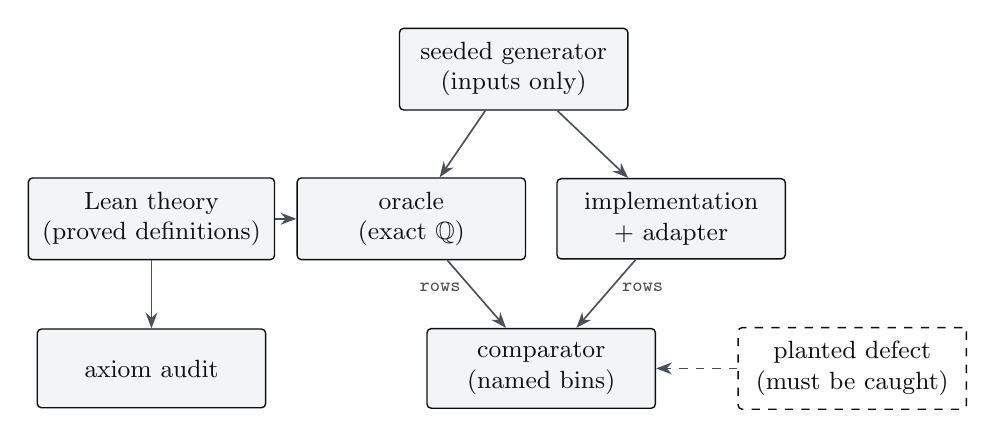
\begin{tikzpicture}[
  box/.style={draw=Ink, line width=0.5pt, fill=Surface, text=Ink, rounded corners=1.5pt,
    align=center, font=\small, inner sep=5pt, minimum height=10mm, minimum width=29mm},
  arr/.style={-{Stealth[length=2mm]}, line width=0.6pt, draw=InkMuted},
  lab/.style={font=\ttfamily\scriptsize, text=InkMuted}]
\node[box] (gen) at (4.6,1.9) {seeded generator\\(inputs only)};
\node[box] (theory) at (0,0) {Lean theory\\(proved definitions)};
\node[box] (oracle) at (3.3,0) {oracle\\(exact $\mathbb{Q}$)};
\node[box] (impl) at (6.6,0) {implementation\\+ adapter};
\node[box] (cmp) at (4.95,-1.9) {comparator\\(named bins)};
\node[box] (audit) at (0,-1.9) {axiom audit};
\node[box, dashed, fill=Background] (planted) at (8.9,-1.9) {planted defect\\(must be caught)};
\draw[arr] (gen) -- (oracle);
\draw[arr] (gen) -- (impl);
\draw[arr] (theory) -- (oracle);
\draw[arr] (theory) -- (audit);
\draw[arr] (oracle) -- node[left, lab, pos=0.4] {rows} (cmp);
\draw[arr] (impl) -- node[right, lab, pos=0.4] {rows} (cmp);
\draw[arr, dashed] (planted) -- (cmp);
\end{tikzpicture}
\caption{The measurement procedure. The generator never computes expected results;
those come only from the oracle.}
\label{fig:harness}
\end{figure}

The procedure follows \texttt{ledger-semantics} (\cref{fig:harness}). A seeded
generator writes case files containing inputs only. It favors the inputs where
implementations are known to have conventions: tied logits, words that are
themselves tokens, and merge tables with several splits of one string. A small
adapter per implementation runs the same cases and prints the oracle's row format.
The comparator places every case in exactly one named bin (agree, diverge, skipped
by either side, or missing), so nothing is dropped silently. Token rows are compared
as strings. Sampler rows require that a zero be matched by a zero and that nonzero
probabilities agree within $10^{-6}$, since llama.cpp stores logits in
\texttt{float32}. Each comparator is observed to fail: a planted defect, an adapter
that glues two tokens or one that inverts temperature, must be detected or the run
fails.

\paragraph{Tie divergences.} An implementation that keeps exactly $k$ tokens breaks
ties in its own order, which need not be the oracle's order by index. Every filter
treats tied tokens alike except for that choice, and tied tokens stay tied through
temperature and renormalization. Such an implementation must therefore agree with
the positional semantics up to a permutation of tied tokens. The harness checks
exactly this: the multiset of (logit, probability) pairs over the kept tokens must
equal that of the oracle's \texttt{q} rows. A divergence that fails this check is
reported as unexplained.

\begin{table}[t]
\centering\small
\caption{Measurements (\texttt{harness/run.sh 600}: four seeds of 600 cases each per
corpus). Lean 4.34.1, Mathlib v4.34.1, \texttt{tokenizers} 0.23.3, \texttt{tiktoken}
0.14.0, llama.cpp commit \texttt{a9d27ac} (2026-10-11).}
\label{tab:results}
\begin{tabularx}{\linewidth}{@{}>{\raggedright\arraybackslash}p{4.6cm}>{\raggedright\arraybackslash}X>{\raggedright\arraybackslash}X@{}}
\toprule
\qpth{Implementation} & \qpth{Compared against} & \qpth{Result}\\
\midrule
HF \texttt{tokenizers}, BPE, defaults & rule-rank BPE (\lean{bpe}) & 13{,}779 / 13{,}779 words identical\\
HF \texttt{tokenizers}, \lean{ignore_merges} & lookup, then rule-rank BPE & 13{,}779 / 13{,}779 identical\\
\texttt{tiktoken} & lookup, then concatenation-rank BPE & 13{,}779 / 13{,}779 identical\\
llama.cpp \lean{top_k}, \lean{top_p}, \lean{min_p}, \texttt{temp}, no ties & tie-keeping filters & 1{,}216 / 1{,}216 chains, $|\Delta p|\le5.1\times10^{-8}$\\
llama.cpp, with ties & tie-keeping, else positional & 939 + 245 / 1{,}184 chains; 0 unexplained\\
Planted defects (tokenizer, sampler) & --- & both detected\\
\bottomrule
\end{tabularx}
\end{table}

\Cref{tab:results} summarizes the results. Two findings came out of the
comparisons. First, \texttt{tiktoken} initially disagreed with the oracle's
concatenation-rank BPE on words that are themselves vocabulary tokens. The
disagreement was a convention, whole-word lookup. Following the
\texttt{ledger-semantics} rule that a divergence is either a defect in the
implementation or a convention the semantics has not yet recorded, we recorded it
as \lean{lookupFirst}, with its own theorems, after which agreement is exact.
Second, on the same random merge tables the two tokenizer libraries disagree with
each other on 439 of 13{,}779 words (3.2\%), and on 279 when Hugging Face uses
\lean{ignore_merges}. The oracle reproduces each library exactly, so every one of
these disagreements is predicted. \Cref{thm:bpeconv} states the condition under which
they cannot occur.

For sampling, llama.cpp agrees with the tie-keeping semantics on every tie-free
chain. On chains with ties, 245 of 1{,}184 diverge, and every one agrees with the
positional semantics up to a permutation of tied tokens. Some of these divergences
cascade: a tie cut by top-$k$ changes the renormalized masses that a later top-$p$
sees. A check that compared kept sets only after the fact would misclassify such
cases. Replaying the convention exactly classifies all of them.

% ===========================================================================
\section{Related work}

\paragraph{Formal methods for machine learning.} Most verification work on neural
networks proves properties of trained models, for example with SMT-based
methods~\cite{katz2017reluplex}. We verify the model-independent algorithms around
the model instead, and connect them to implementations through an oracle. The
denotational method follows Elliott~\cite{elliott2009denotational}. The use of a
proved semantics as a test oracle, the procedure of planted defects, and the
discipline of named skip bins follow \texttt{ledger-semantics}~\cite{ledgersemantics}.
Our category of finite stochastic maps is a special case of Fritz's Markov
categories~\cite{fritz2020markov}.

\paragraph{Tokenization.} Zouhar et al.\ give a formal analysis of BPE as an
optimization problem~\cite{zouhar2023bpe}. Gastaldi et al.\ treat tokenizers as
stochastic maps and study consistency of estimators~\cite{gastaldi2024foundations}.
Vieira et al.\ show how to turn token-level models into character-level
ones~\cite{vieira2024tokens}, which requires exactly the enumeration of
tokenizations we verify. Our no-compression theorem and the agreement criterion
between BPE conventions complement this work at the level of exact identities.

\paragraph{Decoding.} Top-$k$~\cite{fan2018hierarchical}, nucleus~\cite{holtzman2020curious}
and min-$p$~\cite{nguyen2025minp} sampling are usually specified by an algorithm over
sorted arrays, which leaves ties unspecified. \Cref{thm:topk} shows that this gap
cannot be closed by any symmetric rule. Speculative
sampling~\cite{leviathan2023speculative,chen2023speculative} is known to be lossless,
and its acceptance rate is the maximal-coupling bound~\cite{lindvall1992coupling}. Du et
al.\ characterize tightness measure-theoretically~\cite{du2023tight}. We give a
finite-depth statement and an explicit non-tight model.

\paragraph{Attention and inference systems.} Online softmax~\cite{milakov2018online}
underlies FlashAttention~\cite{dao2022flashattention} and its successors, and
KV caching is standard in serving systems~\cite{pope2023scaling,kwon2023vllm}. Our
contribution is the algebraic packaging, a commutative monoid with a free-monoid
homomorphism, and machine-checked proofs over arbitrary exponential characters.
Permutation equivariance of attention without positional encodings is
known~\cite{yun2020universal}.

\paragraph{Masked diffusion.} The time-independence of the optimal denoiser was
observed by Ou et al.~\cite{ou2025absorbing}, in the setting of
D3PM~\cite{austin2021d3pm}, MDLM~\cite{sahoo2024mdlm} and related
models~\cite{shi2024masked,nie2025llada}. We machine-check it, together with the
any-order chain rule and the inexactness of parallel unmasking.

% ===========================================================================
\section{Limitations}

Analysis on the reals enters only through exponential characters, and there is no
measure theory, so sampling and tightness are stated through finite quantities. The
oracle's temperature is restricted to $1/n$, which keeps softmax rational. The
theorems hold for every temperature, but the oracle cannot evaluate an irrational
softmax. Speculative decoding is proved for one drafted token. The sequence version
follows by induction and is not yet formalized. Nothing is proved about
floating-point arithmetic: implementations are compared with exact values within a
stated tolerance. A decision that lies exactly on a floating-point boundary could in
principle diverge, and none occurred in our runs. The diffusion theory covers
absorbing diffusion, not Gaussian diffusion. The chat protocol models tool calling in
its common request-and-result form, not any vendor's specification. The measurements
cover tokenizers and samplers; attention kernels, speculative decoders, chat
renderers and diffusion samplers are evaluated by the oracle but not yet compared
against implementations.

% ===========================================================================
\section{Conclusion}

The inference side of LLMs is small enough to be given a precise meaning and large
enough that its implementations disagree. A machine-checked semantics separates
what is meaning from what is convention. It proves which reorderings, cachings and
tilings are harmless, and it shows that some properties folklore expects, such as
symmetric exact top-$k$, compositional compressing tokenizers and unambiguous plain-text
templates, cannot exist. Connected to an exact oracle, the same definitions become
a test instrument. Every divergence it surfaces is either a defect in an
implementation or a convention that belongs in the semantics.

\paragraph{Availability.} The Lean development, oracle, harness, and recorded
measurement log accompany this paper.

\paragraph{Acknowledgments.} The structure of this work follows
\texttt{ledger-semantics} by John Wiegley. The formalization and harness were
developed with the assistance of an AI system (Claude, Anthropic).

% ===========================================================================
\begin{thebibliography}{99}\small

\bibitem{austin2021d3pm}
J.~Austin, D.~D. Johnson, J.~Ho, D.~Tarlow, and R.~van~den Berg.
\newblock Structured denoising diffusion models in discrete state-spaces.
\newblock In \emph{NeurIPS}, 2021.

\bibitem{chen2023speculative}
C.~Chen, S.~Borgeaud, G.~Irving, J.-B. Lespiau, L.~Sifre, and J.~Jumper.
\newblock Accelerating large language model decoding with speculative sampling.
\newblock arXiv:2302.01318, 2023.

\bibitem{dao2022flashattention}
T.~Dao, D.~Y. Fu, S.~Ermon, A.~Rudra, and C.~R{\'e}.
\newblock {FlashAttention}: Fast and memory-efficient exact attention with {IO}-awareness.
\newblock In \emph{NeurIPS}, 2022.

\bibitem{demoura2021lean4}
L.~de~Moura and S.~Ullrich.
\newblock The {Lean} 4 theorem prover and programming language.
\newblock In \emph{CADE-28}, 2021.

\bibitem{du2023tight}
L.~Du, L.~Torroba~Hennigen, T.~Pimentel, C.~Meister, J.~Eisner, and R.~Cotterell.
\newblock A measure-theoretic characterization of tight language models.
\newblock In \emph{ACL}, 2023.

\bibitem{elliott2009denotational}
C.~Elliott.
\newblock Denotational design with type class morphisms.
\newblock Technical Report 2009-01, LambdaPix, 2009.

\bibitem{fan2018hierarchical}
A.~Fan, M.~Lewis, and Y.~Dauphin.
\newblock Hierarchical neural story generation.
\newblock In \emph{ACL}, 2018.

\bibitem{fritz2020markov}
T.~Fritz.
\newblock A synthetic approach to {Markov} kernels, conditional independence and theorems on sufficient statistics.
\newblock \emph{Advances in Mathematics}, 370, 2020.

\bibitem{gastaldi2024foundations}
J.~L. Gastaldi, J.~Terilla, L.~Malagutti, B.~DuSell, T.~Vieira, and R.~Cotterell.
\newblock The foundations of tokenization: Statistical and computational concerns.
\newblock arXiv:2407.11606, 2024.

\bibitem{greshake2023injection}
K.~Greshake, S.~Abdelnabi, S.~Mishra, C.~Endres, T.~Holz, and M.~Fritz.
\newblock Not what you've signed up for: Compromising real-world {LLM}-integrated applications with indirect prompt injection.
\newblock In \emph{AISec}, 2023.

\bibitem{holtzman2020curious}
A.~Holtzman, J.~Buys, L.~Du, M.~Forbes, and Y.~Choi.
\newblock The curious case of neural text degeneration.
\newblock In \emph{ICLR}, 2020.

\bibitem{katz2017reluplex}
G.~Katz, C.~Barrett, D.~L. Dill, K.~Julian, and M.~J. Kochenderfer.
\newblock Reluplex: An efficient {SMT} solver for verifying deep neural networks.
\newblock In \emph{CAV}, 2017.

\bibitem{kwon2023vllm}
W.~Kwon, Z.~Li, S.~Zhuang, Y.~Sheng, L.~Zheng, C.~H. Yu, J.~E. Gonzalez, H.~Zhang, and I.~Stoica.
\newblock Efficient memory management for large language model serving with {PagedAttention}.
\newblock In \emph{SOSP}, 2023.

\bibitem{ledgersemantics}
J.~Wiegley.
\newblock ledger-semantics: Mathematical semantics of {Ledger}, the double-entry accounting tool.
\newblock \url{https://github.com/ledger/ledger-semantics}, 2026.

\bibitem{leviathan2023speculative}
Y.~Leviathan, M.~Kalman, and Y.~Matias.
\newblock Fast inference from transformers via speculative decoding.
\newblock In \emph{ICML}, 2023.

\bibitem{lindvall1992coupling}
T.~Lindvall.
\newblock \emph{Lectures on the Coupling Method}.
\newblock Wiley, 1992.

\bibitem{liu2023ring}
H.~Liu, M.~Zaharia, and P.~Abbeel.
\newblock Ring attention with blockwise transformers for near-infinite context.
\newblock arXiv:2310.01889, 2023.

\bibitem{mathlib2020}
The mathlib Community.
\newblock The {Lean} mathematical library.
\newblock In \emph{CPP}, 2020.

\bibitem{milakov2018online}
M.~Milakov and N.~Gimelshein.
\newblock Online normalizer calculation for softmax.
\newblock arXiv:1805.02867, 2018.

\bibitem{nguyen2025minp}
M.~N. Nguyen, A.~Baker, C.~Neo, A.~Roush, A.~Kirsch, and R.~Shwartz-Ziv.
\newblock Turning up the heat: Min-p sampling for creative and coherent {LLM} outputs.
\newblock In \emph{ICLR}, 2025.

\bibitem{nie2025llada}
S.~Nie, F.~Zhu, Z.~You, X.~Zhang, J.~Ou, J.~Hu, J.~Zhou, Y.~Lin, J.-R. Wen, and C.~Li.
\newblock Large language diffusion models.
\newblock arXiv:2502.09992, 2025.

\bibitem{ou2025absorbing}
J.~Ou, S.~Nie, K.~Xue, F.~Zhu, J.~Sun, Z.~Li, and C.~Li.
\newblock Your absorbing discrete diffusion secretly models the conditional distributions of clean data.
\newblock In \emph{ICLR}, 2025.

\bibitem{pope2023scaling}
R.~Pope, S.~Douglas, A.~Chowdhery, J.~Devlin, J.~Bradbury, J.~Heek, K.~Xiao, S.~Agrawal, and J.~Dean.
\newblock Efficiently scaling transformer inference.
\newblock In \emph{MLSys}, 2023.

\bibitem{rabe2021selfattention}
M.~N. Rabe and C.~Staats.
\newblock Self-attention does not need {$O(n^2)$} memory.
\newblock arXiv:2112.05682, 2021.

\bibitem{radford2019gpt2}
A.~Radford, J.~Wu, R.~Child, D.~Luan, D.~Amodei, and I.~Sutskever.
\newblock Language models are unsupervised multitask learners.
\newblock OpenAI technical report, 2019.

\bibitem{sahoo2024mdlm}
S.~S. Sahoo, M.~Arriola, Y.~Schiff, A.~Gokaslan, E.~Marroquin, J.~T. Chiu, A.~Rush, and V.~Kuleshov.
\newblock Simple and effective masked diffusion language models.
\newblock In \emph{NeurIPS}, 2024.

\bibitem{sennrich2016bpe}
R.~Sennrich, B.~Haddow, and A.~Birch.
\newblock Neural machine translation of rare words with subword units.
\newblock In \emph{ACL}, 2016.

\bibitem{shi2024masked}
J.~Shi, K.~Han, Z.~Wang, A.~Doucet, and M.~K. Titsias.
\newblock Simplified and generalized masked diffusion for discrete data.
\newblock In \emph{NeurIPS}, 2024.

\bibitem{vieira2024tokens}
T.~Vieira, B.~LeBrun, M.~Giulianelli, J.~L. Gastaldi, B.~DuSell, J.~Terilla, T.~J. O'Donnell, and R.~Cotterell.
\newblock From language models over tokens to language models over characters.
\newblock arXiv:2412.03719, 2024.

\bibitem{wolf2020transformers}
T.~Wolf et~al.
\newblock Transformers: State-of-the-art natural language processing.
\newblock In \emph{EMNLP: System Demonstrations}, 2020.

\bibitem{xiao2024sinks}
G.~Xiao, Y.~Tian, B.~Chen, S.~Han, and M.~Lewis.
\newblock Efficient streaming language models with attention sinks.
\newblock In \emph{ICLR}, 2024.

\bibitem{yun2020universal}
C.~Yun, S.~Bhojanapalli, A.~S. Rawat, S.~J. Reddi, and S.~Kumar.
\newblock Are transformers universal approximators of sequence-to-sequence functions?
\newblock In \emph{ICLR}, 2020.

\bibitem{zouhar2023bpe}
V.~Zouhar, C.~Meister, J.~L. Gastaldi, L.~Du, T.~Vieira, M.~Sachan, and R.~Cotterell.
\newblock A formal perspective on byte-pair encoding.
\newblock In \emph{Findings of ACL}, 2023.

\end{thebibliography}

\end{document}
"
% ---------------------------------------------------------------------------
\documentclass[10pt]{article}

\newif\ifqptdark
\qptdarkfalse   % print edition (light). \qptdarktrue gives the dark screen edition.
\ifdefined\qptdarkedition\qptdarktrue\fi  % or: xelatex "\def\qptdarkedition{}% !TeX program = xelatex
% ---------------------------------------------------------------------------
%  A Machine-Checked Semantics of LLM Inference
%  Daniel Arango Sohm, Universidad EAFIT
%
%  Typeset in the QPT visual design system:
%    * neutral-first: Ink on Background carries the document;
%    * paradigm colours are semantic only. This paper belongs to none of the
%      five paradigms, so no paradigm colour appears in its content; the
%      colours appear only in the QPT mark itself;
%    * no gradients;
%    * Space Grotesk for display, Inter for body text, IBM Plex Mono for
%      technical, numeric, label, code and proof-oriented content.
%
%  Compile with:  xelatex llm-semantics-qpt.tex   (twice, for references)
%  Dark screen edition: set \qptdarktrue below, or run
%    xelatex -jobname=llm-semantics-qpt-dark "\def\qptdarkedition{}\input{llm-semantics-qpt}"
% ---------------------------------------------------------------------------
\documentclass[10pt]{article}

\newif\ifqptdark
\qptdarkfalse   % print edition (light). \qptdarktrue gives the dark screen edition.
\ifdefined\qptdarkedition\qptdarktrue\fi  % or: xelatex "\def\qptdarkedition{}\input{llm-semantics-qpt}"

\usepackage[a4paper,textwidth=15.4cm,textheight=23.6cm,top=3.0cm,headsep=0.9cm,footskip=1.2cm]{geometry}
\usepackage{amsmath,amssymb,amsthm,mathtools}
\usepackage{fontspec}
\usepackage{booktabs,tabularx,array}
\usepackage[protrusion=true,expansion=false]{microtype}
\usepackage[table]{xcolor}
\usepackage{graphicx}
\usepackage{fvextra}
\usepackage{enumitem}
\usepackage{caption}
\usepackage{titlesec}
\usepackage{fancyhdr}
\usepackage[most]{tcolorbox}
\usepackage{tikz}
\usetikzlibrary{arrows.meta}
\usepackage{hyperref}
\usepackage[nameinlink,capitalise]{cleveref}

% ---------------------------------------------------------------------------
%  Colour tokens
% ---------------------------------------------------------------------------
% Neutral foundation. Ink and Background invert between the two editions.
\ifqptdark
  \definecolor{Background}{HTML}{0B0C0E}
  \definecolor{Surface}{HTML}{16181B}
  \definecolor{Border}{HTML}{2B2E33}
  \definecolor{Ink}{HTML}{EDEEF0}
  \definecolor{InkMuted}{HTML}{A9AEB6}
  \definecolor{InkFaint}{HTML}{5A5F67}   % decoration only, never meaningful text
\else
  \definecolor{Background}{HTML}{FFFFFF}
  \definecolor{Surface}{HTML}{F3F4F5}
  \definecolor{Border}{HTML}{DADDE1}
  \definecolor{Ink}{HTML}{0E0F11}
  \definecolor{InkMuted}{HTML}{4B4F57}
  \definecolor{InkFaint}{HTML}{A3A7AE}   % decoration only, never meaningful text
\fi
% Paradigm colours: fixed in both editions, semantic only.
\definecolor{Quantum}{HTML}{5BAD1E}
\definecolor{Photonic}{HTML}{F0AB00}
\definecolor{Thermodynamic}{HTML}{E8690A}
\definecolor{Ternary}{HTML}{8A8A8A}
\definecolor{Bio}{HTML}{1AAB7C}

\ifqptdark\pagecolor{Background}\fi

% ---------------------------------------------------------------------------
%  Typography
% ---------------------------------------------------------------------------
\setmainfont{Inter}[
  Path=fonts/, Extension=.otf, Scale=0.94,
  UprightFont=*-Regular, ItalicFont=*-Italic,
  BoldFont=*-SemiBold, BoldItalicFont=*-SemiBoldItalic]
\setmonofont{IBMPlexMono}[
  Path=fonts/, Extension=.ttf, Scale=MatchLowercase,
  UprightFont=*-Regular, ItalicFont=*-Italic, BoldFont=*-SemiBold]
\newfontfamily\qptdisplay{SpaceGrotesk}[
  Path=fonts/, Extension=.otf, UprightFont=*-Medium, BoldFont=*-Bold]
\newfontfamily\qptdisplaylight{SpaceGrotesk}[
  Path=fonts/, Extension=.otf, UprightFont=*-Regular]
\newfontfamily\qptlabelfont{IBMPlexMono}[
  Path=fonts/, Extension=.ttf, Scale=MatchLowercase, UprightFont=*-Medium,
  LetterSpace=6]
\setsansfont{Inter}[
  Path=fonts/, Extension=.otf, Scale=0.94,
  UprightFont=*-Regular, ItalicFont=*-Italic,
  BoldFont=*-SemiBold, BoldItalicFont=*-SemiBoldItalic]
\linespread{1.16}
\setlength{\emergencystretch}{2.5em}
\AtBeginDocument{\raggedright\setlength{\parindent}{0pt}}
\setlength{\parindent}{0pt}
\setlength{\parskip}{0.55em}

% A label: IBM Plex Mono, upper case, tracked.
\newcommand{\qptlabel}[1]{{\qptlabelfont\footnotesize\MakeUppercase{#1}}}
% Technical names (Lean declarations, files) in IBM Plex Mono.
\newcommand{\lean}[1]{\texttt{\detokenize{#1}}}
\newcommand{\leanref}[1]{\par\smallskip\noindent
  {\ttfamily\footnotesize\upshape\raggedright\color{InkMuted}LEAN\enspace #1\par}}

% Ink is the normal colour everywhere, including floats, heads and footnotes.
\makeatletter
\AtBeginDocument{\color{Ink}\global\let\default@color\current@color}
\makeatother

% ---------------------------------------------------------------------------
%  Mathematical notation
% ---------------------------------------------------------------------------
\newcommand{\K}{\Bbbk}
\newcommand{\Dist}{\mathrm{Dist}}
\newcommand{\restr}[2]{#1|_{#2}}
\newcommand{\topk}{\mathrm{TopK}}
\newcommand{\topp}{\mathrm{TopP}}
\newcommand{\minp}{\mathrm{MinP}}
\newcommand{\sharpen}{\mathrm{sharpen}}
\newcommand{\abv}{\mathrm{above}}
\newcommand{\tv}{\mathrm{tv}}
\newcommand{\dec}{\mathrm{dec}}
\newcommand{\enc}{\mathrm{enc}}
\newcommand{\softmax}{\mathrm{softmax}}
\newcommand{\attend}{\mathrm{attend}}
\newcommand{\Iv}[1]{[\![#1]\!]}
\newcommand{\Mask}{\bot}

% ---------------------------------------------------------------------------
%  Headings: section numbers as labels, titles in Space Grotesk
% ---------------------------------------------------------------------------
\makeatletter
\newcommand{\qptsecnum}[1]{{\qptlabelfont\small\color{InkMuted}\two@digits{#1}}}
\makeatother
\titleformat{\section}
  {\qptdisplay\fontsize{14.5}{18}\selectfont\color{Ink}}
  {\qptsecnum{\value{section}}}{0.9em}{}
\titleformat{name=\section,numberless}
  {\qptdisplay\fontsize{14.5}{18}\selectfont\color{Ink}}{}{0pt}{}
\titlespacing*{\section}{0pt}{1.9em}{0.7em}
\titleformat{\paragraph}[runin]
  {\qptdisplay\normalsize\color{Ink}}{}{0pt}{}
\titlespacing*{\paragraph}{0pt}{0.9em}{0.6em}

% ---------------------------------------------------------------------------
%  Statements
% ---------------------------------------------------------------------------
\newtheoremstyle{qpt}
  {0.9em}{0.9em}
  {\normalfont}{}
  {\qptlabelfont\footnotesize}{}
  {\newline}
  {\MakeUppercase{\thmname{#1}\thmnumber{~#2}}%
   \thmnote{\enspace{\qptdisplay\normalsize\color{Ink}#3}}}
\theoremstyle{qpt}
\newtheorem{theorem}{Theorem}
\newtheorem{proposition}[theorem]{Proposition}
\newtheorem{corollary}[theorem]{Corollary}
\newtheorem{lemma}[theorem]{Lemma}
\newtheorem{definition}[theorem]{Definition}
\newtheorem{remark}[theorem]{Remark}

% Proofs: a tracked label and a neutral end mark.
\makeatletter
\renewcommand{\qedsymbol}{{\color{InkMuted}\rule{0.5em}{0.5em}}}
\renewenvironment{proof}[1][Proof]{\par\pushQED{\qed}\normalfont\topsep0.5em\relax
  \trivlist\item[\hskip\labelsep\qptlabel{#1}\hspace{0.6em}]\ignorespaces}
  {\popQED\endtrivlist\@endpefalse}
\makeatother

% ---------------------------------------------------------------------------
%  Code: IBM Plex Mono on a neutral surface, with a hairline on the left
% ---------------------------------------------------------------------------
\tcbset{colupper=Ink, collower=Ink}
\tcbset{qptcode/.style={enhanced, colback=Surface, colframe=Surface,
  boxrule=0pt, arc=0pt, left=9pt, right=8pt, top=5pt, bottom=5pt,
  borderline west={1.2pt}{0pt}{InkFaint}, before skip=0.7em, after skip=0.7em}}
\newenvironment{leancode}
  {\VerbatimEnvironment\begin{tcolorbox}[qptcode]%
   \begin{Verbatim}[fontsize=\small,commandchars=\\\{\},
     codes={\catcode`\$=3\catcode`\^=7},formatcom=\color{Ink}]}
  {\end{Verbatim}\end{tcolorbox}}
\newenvironment{casecode}
  {\VerbatimEnvironment\begin{tcolorbox}[qptcode,before skip=0pt,after skip=0pt]%
   \begin{Verbatim}[fontsize=\footnotesize,formatcom=\color{Ink}]}
  {\end{Verbatim}\end{tcolorbox}}

% ---------------------------------------------------------------------------
%  Floats, tables, captions
% ---------------------------------------------------------------------------
\DeclareCaptionLabelFormat{qpt}{\qptlabel{#1~#2}}
\DeclareCaptionLabelSeparator{qptsep}{\quad}
\captionsetup{labelformat=qpt, labelsep=qptsep, font={small,color=Ink},
  justification=raggedright, singlelinecheck=false, skip=6pt}
\newcommand{\qpth}[1]{\qptlabel{#1}}
\arrayrulecolor{Ink}
\setlength{\heavyrulewidth}{0.7pt}
\setlength{\lightrulewidth}{0.35pt}
\renewcommand{\arraystretch}{1.22}

% ---------------------------------------------------------------------------
%  Running heads
% ---------------------------------------------------------------------------
\pagestyle{fancy}
\fancyhf{}
\fancyhead[L]{{\color{Ink}\qptlabel{Machine-checked semantics of LLM inference}}}
\fancyhead[R]{{\color{Ink}\qptlabel{D. Arango Sohm}}}
\fancyfoot[R]{{\ttfamily\small\color{InkMuted}\thepage}}
\renewcommand{\headrule}{{\color{Border}\hrule height 0.4pt}\vspace{-0.4pt}}
\renewcommand{\headrulewidth}{0.4pt}
\fancypagestyle{qptfirst}{\fancyhf{}%
  \fancyfoot[R]{{\ttfamily\small\color{InkMuted}\thepage}}%
  \renewcommand{\headrulewidth}{0pt}\renewcommand{\headrule}{}}

% ---------------------------------------------------------------------------
%  Links and references: neutral, never accent-coloured text
% ---------------------------------------------------------------------------
\hypersetup{colorlinks=true, linkcolor=Ink, citecolor=Ink, urlcolor=Ink,
  pdftitle={A Machine-Checked Semantics of LLM Inference},
  pdfauthor={Daniel Arango Sohm},
  pdfsubject={Formal semantics of large language model inference in Lean 4},
  pdfkeywords={Lean 4, Mathlib, formal verification, LLM inference, sampling,
    tokenization, attention, speculative decoding, diffusion language models}}
\makeatletter
\renewcommand{\@biblabel}[1]{{\ttfamily\color{InkMuted}[#1]}}
\renewcommand{\@cite}[2]{{\ttfamily[#1\if@tempswa, #2\fi]}}
\makeatother
\renewcommand{\refname}{References}

\setlist{itemsep=2pt, topsep=4pt}
\setlist[itemize]{label={\color{InkMuted}\textbullet}}

\begin{document}
\thispagestyle{qptfirst}

% ----------------------------------------------------------------- masthead
\noindent
\begin{minipage}[c]{0.5\linewidth}
  \includegraphics[height=1.9cm]{qpt-logo.png}
\end{minipage}%
\begin{minipage}[c]{0.5\linewidth}\raggedleft
  \qptlabel{Preprint}\\[2pt]
  \qptlabel{October 2026}
\end{minipage}

\vspace{1.6em}
{\color{Border}\rule{\linewidth}{0.4pt}}
\vspace{1.1em}

{\qptdisplay\fontsize{25}{29.5}\selectfont\color{Ink}
A Machine-Checked Semantics\\ of LLM Inference\par}
\vspace{0.55em}
{\qptdisplaylight\fontsize{13}{17}\selectfont\color{InkMuted}
Sampling, Attention, Tokenization, Chat, Decoding,\\ and Diffusion in Lean~4\par}

\vspace{1.5em}
{\large\bfseries Daniel Arango Sohm}\par
\vspace{0.15em}
{\color{InkMuted}Universidad EAFIT, Medellín, Colombia\\
Former member of the QPT team}\par

\vspace{1.4em}
% ----------------------------------------------------------------- abstract
\begin{tcolorbox}[enhanced, colback=Surface, colframe=Surface, colupper=Ink, boxrule=0pt,
  arc=0pt, left=12pt, right=12pt, top=9pt, bottom=10pt]
\qptlabel{Abstract}\par\vspace{0.35em}
{\small
The inference side of a large language model is a stack of small algorithms:
tokenizers, attention kernels, key--value caches, sampling filters, speculative
decoders, chat templates, and diffusion samplers. Each has several independent
implementations, and those implementations are usually tested against one another
rather than against a definition. We give these components a single mathematical
semantics, formalized in Lean~4 against Mathlib. The development comprises about
4{,}600 lines and 270 named theorems, and every declaration depends only on Lean's
three standard axioms. It proves the exact algebra of sampling filters, the
losslessness and optimality of speculative sampling, and the correctness of
key--value caching and of FlashAttention-style online softmax as a commutative
monoid. It proves that byte-pair encoding is lossless under every merge priority,
together with a decidable criterion for when the Hugging Face and \texttt{tiktoken}
conventions agree, a protocol checker for tool calls, and the time-independence of
the masked-diffusion denoiser. It also proves six negative results. No sampling
rule that treats tokens symmetrically can always keep exactly $k$ tokens. No
tokenizer that compresses can respect concatenation. Every chat template that writes
its role markers in the content alphabet is ambiguous. No transformer without
positional information can copy a fixed position. An autoregressive model need not
define a distribution over strings. Parallel unmasking in diffusion is inexact.
From the same definitions we build an executable oracle that evaluates test cases in
exact rational arithmetic, and a harness that measures implementations against it.
On 2{,}400 random merge tables, Hugging Face \texttt{tokenizers} and
\texttt{tiktoken} each agree with the oracle on all 13{,}779 test words, while
disagreeing with each other on 3.2\% of them. On 2{,}400 random sampler chains,
every divergence of llama.cpp from the tie-keeping semantics is accounted for
exactly by the positional semantics that the impossibility theorem forces.
\par}
\end{tcolorbox}

\vspace{0.3em}
\noindent\qptlabel{Keywords}\enspace{\small Lean~4 · Mathlib · formal verification ·
LLM inference · sampling · tokenization · attention · speculative decoding ·
diffusion language models}

\vspace{0.4em}
{\color{Border}\rule{\linewidth}{0.4pt}}

% ===========================================================================
\section{Introduction}

A deployed language model is a function from parameters and a context to a
distribution over tokens. Turning that distribution into text requires more
machinery. A tokenizer maps strings to token sequences. Attention kernels compute
the model's reads over a cached context. A chain of sampling filters reshapes the
next-token distribution. A speculative decoder may verify drafted tokens, a chat
template linearizes a conversation, and a diffusion sampler may unmask several
positions at once. Each of these components exists in many implementations, such as
Hugging Face \texttt{transformers} and \texttt{tokenizers}~\cite{wolf2020transformers},
\texttt{tiktoken}, vLLM~\cite{kwon2023vllm}, and llama.cpp. Their tests mostly
compare one implementation with another, or with remembered behavior.

This paper follows a different discipline, \emph{denotational design}~\cite{elliott2009denotational}.
One first says precisely what a thing means, then requires every operation to
preserve that meaning, and lets the implementation be whatever the equations force
it to be. The approach is that of \texttt{ledger-semantics}~\cite{ledgersemantics},
which formalizes double-entry accounting in Lean and uses the result as a test oracle
for the C++ Ledger program. We apply it to LLM inference. A sampling filter means
conditioning a distribution on a set. A KV-cached decoder means causal attention over
the whole prefix. A FlashAttention kernel means a softmax-weighted average. A chat
template means an injective encoding of a transcript. The theorems state when an
implementation preserves that meaning, and several of them state that no
implementation can.

\paragraph{Contributions.}
\begin{itemize}[leftmargin=*,itemsep=2pt]
\item A Lean~4 formalization against Mathlib~\cite{mathlib2020,demoura2021lean4}
  of sampling, speculative decoding, softmax and attention, tokenization, chat
  transcripts, autoregressive decoding, and masked diffusion
  (\cref{sec:foundations,sec:sampling,sec:spec,sec:attention,sec:tokenization,sec:chat,sec:decoding,sec:diffusion}).
  All definitions are stated over an arbitrary linearly ordered field, so one proof
  covers the real numbers of the literature and the exact rationals of the oracle.
\item Positive results in a common framework. They include the algebra of
  sampling filters, the optimality of speculative sampling, an online-softmax
  commutative monoid, a generic correctness theorem for BPE with a decidable
  agreement criterion between the two conventions in use, a protocol checker for
  tool calls, and the any-order chain rule for masked diffusion.
\item Six negative results that explain design constraints visible across
  implementations (\cref{sec:negative}).
\item An executable oracle that evaluates case files under the proved
  definitions in exact arithmetic, and a measurement of Hugging Face
  \texttt{tokenizers}, \texttt{tiktoken}, and llama.cpp against it (\cref{sec:oracle,sec:measure}).
\end{itemize}

Several of the positive results are known: losslessness of speculative
sampling~\cite{leviathan2023speculative,chen2023speculative}, correctness of online
softmax~\cite{milakov2018online,dao2022flashattention}, time-independence of the
absorbing-diffusion posterior~\cite{ou2025absorbing}, and the role of permutation
equivariance~\cite{yun2020universal}. Our contribution for these is a machine-checked
statement in one framework, connected to an oracle. To our knowledge the
following are not stated elsewhere in the form given here: the impossibility of
symmetric exact top-$k$ and nucleus selection, the no-compression theorem for
homomorphic tokenizers, the ambiguity of every in-band chat template, and the
decidable agreement criterion between merge-rule and concatenation-rank BPE.

% ===========================================================================
\section{Method and trust base}\label{sec:method}

The development is a Lean~4 library (Lean 4.34.1, Mathlib v4.34.1) of eleven
theory modules and two executable modules (\cref{tab:modules}). It is built with
warnings promoted to errors, so an unproved theorem (\lean{sorry}) fails the build.
A separate audit program walks every declaration in the library, 853 in all, and
fails unless each depends only on propositional extensionality, the axiom of choice,
and quotient soundness. The audit has been observed to fail: a planted proof by
\lean{native_decide}, which introduces an auxiliary axiom trusting compiled code, is
rejected. The warnings-as-errors build alone does not catch it. Concrete
counterexamples are therefore proved by \lean{decide}, whose certificate the kernel
checks by evaluation.

\begin{table}[t]
\centering\small
\caption{Modules of the development. Lines and named theorems and lemmas per module.}
\label{tab:modules}
\begin{tabularx}{\linewidth}{@{}l>{\raggedright\arraybackslash}X>{\ttfamily}r>{\ttfamily}r@{}}
\toprule
\qpth{Module} & \qpth{Content} & \qpth{Lines} & \qpth{Thms} \\
\midrule
\lean{Dist} & finite distributions, conditioning, total variation, $\mathsf{FinStoch}$ & 383 & 34\\
\lean{Sampling} & top-$k$, top-$p$, min-$p$, temperature, ties, inverse CDF & 732 & 46\\
\lean{Counterexamples} & kernel-checked failures of sampler laws & 52 & 4\\
\lean{Speculative} & speculative sampling, couplings & 194 & 17\\
\lean{Softmax} & exponential characters, masking, temperature & 220 & 23\\
\lean{Attention} & equivariance, causality, KV cache, online softmax & 573 & 38\\
\lean{Real} & $\exp$ as a character; textbook restatements & 51 & 4\\
\lean{Tokenization} & free-monoid decoding, BPE conventions, enumeration & 860 & 49\\
\lean{Chat} & tool-call protocol, rendering & 440 & 21\\
\lean{Decoding} & mass conservation, tightness, greedy decoding & 245 & 15\\
\lean{Diffusion} & masked diffusion, posterior, chain rule & 379 & 18\\
\lean{Oracle}, \lean{Driver} & case parsing and exact evaluation & 465 & 1\\
\midrule
Total & & 4{,}594 & 270\\
\bottomrule
\end{tabularx}
\end{table}

\paragraph{Numbers.} Every probability lives in an arbitrary field $\K$ with a
compatible linear order (\lean{[Field K] [LinearOrder K] [IsStrictOrderedRing K]}).
The oracle instantiates $\K=\mathbb{Q}$, so its arithmetic is exact. The analytic
statements instantiate $\K=\mathbb{R}$. No measure theory is used. Sampling is made
precise through interval statements (\cref{thm:invcdf}), and tightness through
masses at finite depth (\cref{sec:decoding}).

% ===========================================================================
\section{Foundations}\label{sec:foundations}

\begin{definition}[Finite distribution]
For a finite type $\alpha$, $\Dist_\K(\alpha)$ is the type of functions
$p:\alpha\to\K$ with $p(a)\ge 0$ for all $a$ and $\sum_a p(a)=1$.
\leanref{\lean{Dist}}
\end{definition}

\begin{leancode}
structure Dist ($\K$ : Type u) [Field $\K$] [LinearOrder $\K$] [IsStrictOrderedRing $\K$]
    ($\alpha$ : Type v) [Fintype $\alpha$] where
  prob : $\alpha$ $\to$ $\K$
  nonneg : $\forall$ a, 0 $\le$ prob a
  sum_eq_one : $\sum$ a, prob a = 1
\end{leancode}

The single operation through which masks, filters and grammar constraints act is
conditioning. For $S\subseteq\alpha$ with $p(S)>0$, write
$\restr{p}{S}(a)=\Iv{a\in S}\,p(a)/p(S)$ (\lean{Dist.restrict}).

\begin{lemma}[Conditioning]\label{lem:restrict}
$\restr{(\restr{p}{S})}{T}=\restr{p}{S\cap T}$ whenever the masses involved are
positive. Moreover $\restr{p}{S}=\restr{p}{S'}$ whenever $S$ and $S'$ contain the same
outcomes of positive probability.
\leanref{\lean{restrict_restrict}, \lean{restrict_congr}}
\end{lemma}

The finite distribution monad (point masses and \lean{bind}) satisfies the monad
laws. Finite types and stochastic maps $\alpha\to\Dist_\K(\beta)$ form a category
$\mathsf{FinStoch}_\K$, given as an instance of Mathlib's \lean{Category} whose
composition is Kleisli composition (\lean{FinStoch.category}). Total variation is
$\tv(p,q)=\sum_a\max(0,p(a)-q(a))$. We prove
$\tv(p,q)=\tfrac12\sum_a|p(a)-q(a)|$, $\sum_a\min(p(a),q(a))=1-\tv(p,q)$, and
$\tv(p,q)=0\iff p=q$.

% ===========================================================================
\section{Sampling}\label{sec:sampling}

Let $V$ be a finite vocabulary and $p:V\to\K$. Write
$\abv_p(v)=\{u: p(v)<p(u)\}$ for the tokens strictly preferred to $v$. The three
standard filters keep the sets
\begin{gather*}
\topk_k(p)=\{v: |\abv_p(v)|<k\},\qquad
\minp_m(p)=\{v:\forall u,\; m\,p(u)\le p(v)\},\\
\topp_P(p)=\Bigl\{v: \textstyle\sum_{u\in\abv_p(v)}p(u)<P\Bigr\},
\end{gather*}
and the filtered distribution is the conditioning $\restr{p}{S}$ on the kept set
$S$. For distinct probabilities, $\topp_P$ is the usual rule ``sort in descending
order and keep the shortest prefix whose mass reaches $P$''. With ties, all three
keep every tied token. Temperature $1/n$ is
$\sharpen_n(p)(v)=p(v)^n/\sum_u p(u)^n$, which stays inside $\mathbb{Q}$. In
\cref{sec:attention} we show that it equals $\softmax(n\cdot z)$ when
$p=\softmax(z)$. Every kept set contains a most probable token, provided $k\ge1$,
$P>0$ and $m\le1$, so no filter can produce an empty distribution.

\begin{theorem}[Sampler algebra]\label{thm:algebra}
For $k,k'\ge1$, $m,m'\le1$ and $n\ge1$, and writing filters in the order they are
applied,
\begin{enumerate}[label=(\roman*),itemsep=1pt]
\item top-$k$ then top-$k'$ equals top-$\min(k,k')$;
\item min-$m$ then min-$m'$ equals min-$\max(m,m')$; in particular both filters are idempotent;
\item top-$k$ and min-$m$ commute;
\item top-$k$ and temperature $1/n$ commute.
\end{enumerate}
\leanref{\lean{topK_topK}, \lean{minP_minP}, \lean{topK_minP_comm}, \lean{topK_sharpen_comm}}
\end{theorem}

\begin{proof}[Proof sketch]
All three kept sets are \emph{upward closed}: if $v$ is kept and $p(v)<p(u)$, then
$u$ is kept. Conditioning on an upward-closed set $S$ leaves $\abv(v)$ unchanged for
$v\in S$ (\lean{above_restrict}), and min-$p$ is insensitive to conditioning on a set
that contains a maximizer (\lean{minP_restrict_iff}). Each identity then reduces,
through \cref{lem:restrict}, to an equality of kept sets. For (iv), $x\mapsto x^n$
is strictly increasing on $[0,\infty)$, and top-$k$ depends only on the order of the
scores (\lean{topKSet_congr}).
\end{proof}

The laws one might expect beyond \cref{thm:algebra} are false. With
$p_0=(\tfrac12,\tfrac3{10},\tfrac15)$, the kernel evaluates the following
(\lean{Counterexamples}).

\begin{proposition}[Failed laws]\label{prop:counter}
\leavevmode\vspace{-0.5\baselineskip}
\begin{enumerate}[label=(\roman*),itemsep=1pt]
\item Top-$p$ is not idempotent: one pass of $\topp_{3/5}$ gives token~1 the probability $\tfrac38$, and a second pass gives it~$0$.
\item Top-$p$ does not commute with top-$k$: top-$p$ then top-2 leaves token~1 at $\tfrac38$, while top-2 then top-$p$ removes it.
\item Top-$p$ does not commute with temperature $\tfrac12$: token~1 ends at $\tfrac9{34}$ in one order and at $0$ in the other.
\item Min-$p$ ($m=\tfrac12$) does not commute with temperature $\tfrac12$, with the same numbers.
\end{enumerate}
\end{proposition}

A sampler chain may therefore reorder top-$k$, min-$p$ and temperature only as
\cref{thm:algebra} allows, and may not move top-$p$ at all.

\paragraph{Ties.} Implementations differ on ties, and the difference is forced.
Call a selection rule $\mathrm{sel}:(V\to\K)\to\mathcal{P}(V)$ \emph{equivariant} if
$\mathrm{sel}(p\circ\sigma^{-1})=\sigma[\mathrm{sel}(p)]$ for every permutation
$\sigma$ of $V$, that is, if relabeling the tokens relabels the output.

\begin{theorem}[No symmetric exact top-$k$]\label{thm:topk}
Let $0<k<|V|$. No equivariant selection rule satisfies $|\mathrm{sel}(p)|=k$ for
every distribution $p$.
\leanref{\lean{no_equivariant_exact_topK}}
\end{theorem}
\begin{proof}
On the uniform distribution $u$ we have $u\circ\sigma^{-1}=u$ for every $\sigma$, so
$\mathrm{sel}(u)$ is invariant under all permutations. If it contains some $v$, then
for any $w$ the transposition $(v\,w)$ maps $v$ to $w$, so it contains $w$ too.
Hence $\mathrm{sel}(u)$ is either empty or all of $V$, and neither has $k$ elements.
\end{proof}

\begin{leancode}
theorem no_equivariant_exact_topK [DecidableEq V] \char123{}k : $\mathbb{N}$\char125{}
    (hk0 : 0 < k) (hkn : k < Fintype.card V)
    (sel : (V $\to$ $\K$) $\to$ Finset V) (hsel : Equivariant sel) :
    $\neg$ $\forall$ d : Dist $\K$ V, (sel d.prob).card = k
\end{leancode}

\begin{theorem}[No symmetric smallest nucleus]
Let $V$ be nonempty and $0<P\le1-1/|V|$. No equivariant rule returns, for every
distribution, a set of minimum cardinality among those of mass at least~$P$.
\leanref{\lean{no_equivariant_exact_nucleus}}
\end{theorem}

The tie-keeping filters are equivariant (\lean{topKSet_equivariant}). The other
option is to break ties by position. Define $u\prec_p v$ if $p(u)>p(v)$, or if
$p(u)=p(v)$ and $u<v$, and let the positional filters count predecessors under
$\prec_p$ instead of $\abv_p$ (\lean{Dist.topKPos}, \lean{Dist.topPPos}).

\begin{theorem}[Positional tie-breaking]
Positional top-$k$ keeps exactly $\min(k,|V|)$ tokens. If $p$ is injective, the
positional and tie-keeping filters coincide. For $0<k<|V|$, positional top-$k$ is
not equivariant.
\leanref{\lean{card_topKPosSet}, \lean{topKPosSet_eq_of_injective}, \lean{topPPosSet_eq_of_injective}, \lean{topKPosSet_not_equivariant}}
\end{theorem}

An implementation must therefore choose between keeping exactly $k$ tokens and
treating tokens symmetrically. Hugging Face \texttt{transformers} (read from the
source of version 5.19.0) keeps ties in top-$k$, since it removes only scores
strictly below the $k$-th largest, but breaks them by sort position in top-$p$.
llama.cpp breaks ties by position in both, as measured in \cref{sec:measure}.

\begin{theorem}[Inverse-CDF sampling]\label{thm:invcdf}
Let $F(i)=\sum_{j<i}p(j)$ on $V=\{0,\dots,n-1\}$ and let $\iota(u)$ be the least $i$
with $u<F(i+1)$. For $0\le u<1$, $\iota(u)=i\iff F(i)\le u<F(i+1)$, and
$F(i+1)-F(i)=p(i)$. A uniform $u$ therefore selects $i$ with probability $p(i)$.
\leanref{\lean{invCdf_eq_iff}, \lean{cdf_interval_length}}
\end{theorem}

% ===========================================================================
\section{Speculative decoding}\label{sec:spec}

A draft model proposes $x\sim q$. The target, with distribution $p$, accepts with
probability $a(x)=\min(1,p(x)/q(x))$, and on rejection a token is drawn from the
residual $r=(p-q)^+/\tv(p,q)$~\cite{leviathan2023speculative,chen2023speculative}.
We define the joint law of (draft, emitted token) exactly as the algorithm runs,
\[
\pi(x,y)=q(x)\bigl(a(x)\,\Iv{y=x}+(1-a(x))\,r(y)\bigr).
\]

\begin{theorem}[Speculative sampling]
\leavevmode\vspace{-0.5\baselineskip}
\begin{enumerate}[label=(\roman*),itemsep=1pt]
\item The draft has law $q$: $\sum_y\pi(x,y)=q(x)$.
\item \emph{Losslessness}: the emitted token has law $p$: $\sum_x\pi(x,y)=p(y)$.
\item The acceptance probability is $\sum_x q(x)a(x)=1-\tv(p,q)$, and the emitted token equals the draft with the same probability.
\item \emph{Optimality}: every coupling $\gamma$ of $q$ and $p$ has $\sum_x\gamma(x,x)\le1-\tv(p,q)$.
\end{enumerate}
\leanref{\lean{specJoint_fst}, \lean{specJoint_snd}, \lean{accept_rate}, \lean{specJoint_diag}, \lean{coupling_le}, \lean{spec_optimal}}
\end{theorem}
\begin{proof}[Proof sketch]
Since $q(x)a(x)=\min(p(x),q(x))$, the total rejection probability is $\tv(p,q)$,
and a rejected draft is never re-emitted, because $r(x)=0$ whenever $q(x)>p(x)$. For (iv),
$\gamma(x,x)\le\min(q(x),p(x))$ by the marginal constraints. This is the classical
coupling inequality~\cite{lindvall1992coupling}.
\end{proof}

Because any lossless rule for verifying one drafted token is a coupling, (iv) shows
that speculative sampling has the highest acceptance rate any such rule can achieve.

% ===========================================================================
\section{Softmax and attention}\label{sec:attention}

\begin{definition}[Exponential character]
An \emph{exponential character} from an ordered additive group $G$ of scores into
$\K$ is a strictly increasing map $E:G\to\K$ with $E(a)>0$ and $E(a+b)=E(a)E(b)$.
For $z:\iota\to G$, $\softmax_E(z)_i=E(z_i)/\sum_jE(z_j)$.
\leanref{\lean{ExpChar}}
\end{definition}

$\exp:\mathbb{R}\to\mathbb{R}$ is a character (\lean{ExpChar.real}). So is
$z\mapsto2^z:\mathbb{Z}\to\mathbb{Q}$ (\lean{ExpChar.base2}), which the oracle uses
to evaluate softmax with no rounding. Every result in this section holds for every
character, and so for both.

\begin{theorem}[Softmax]\label{thm:softmax}
\leavevmode\vspace{-0.5\baselineskip}
\begin{enumerate}[label=(\roman*),itemsep=1pt]
\item $\softmax_E(z+c)=\softmax_E(z)$; this licenses subtracting the maximum logit.
\item $\softmax_E(z)_i<\softmax_E(z)_j\iff z_i<z_j$.
\item \emph{Masking is conditioning}: setting logits outside $S$ to $-\infty$ and taking softmax gives $\restr{\softmax_E(z)}{S}$.
\item For $G$ a field and $T>0$, $\topk_k(\softmax_E(z/T))=\topk_k(z)$.
\item $\softmax_E(n\cdot z)=\sharpen_n(\softmax_E(z))$.
\end{enumerate}
\leanref{\lean{softmax_add_const}, \lean{softmax_lt_iff}, \lean{softmaxOn_eq_restrict}, \lean{topK_temperature}, \lean{softmax_nsmul}}
\end{theorem}

\paragraph{One read.} $\attend(s,v)=\sum_j\softmax_E(s)_j\,v_j$ for scores $s$ and
values $v_j$ in a $\K$-module.

\begin{theorem}[Convexity]
For every linear functional $\varphi$ and constant $c$, if $\varphi(v_j)\le c$ for all
$j$ then $\varphi(\attend(s,v))\le c$. If every $v_j=m$, then $\attend(s,v)=m$ for
every $s$.
\leanref{\lean{attend_convex}, \lean{attend_const}}
\end{theorem}

The second statement says attention cannot abstain. Its weights always sum to one,
which is the property that motivates attention-sink tokens~\cite{xiao2024sinks}.

\paragraph{Permutation equivariance.} A map $f:(\iota\to X)\to(\iota\to Y)$ is
equivariant if $f(x\circ\sigma)=f(x)\circ\sigma$ for every permutation~$\sigma$.

\begin{theorem}[Equivariance]
Self-attention with any score function and no positional information is
equivariant. So is any block $y=x+\sum_h\mathrm{attn}_h(\mathrm{norm}\,x)$,
$\mathrm{out}=y+\mathrm{mlp}(\mathrm{norm}\,y)$, and any stack of such blocks.
\leanref{\lean{selfAttn_equivariant}, \lean{block_equivariant}, \lean{stack_equivariant}}
\end{theorem}

\begin{theorem}[Positional information is necessary]\label{thm:nofirst}
If $\iota$ has two distinct positions $i_0\ne i_1$ and $X$ has two distinct elements,
no equivariant $f:(\iota\to X)\to(\iota\to X)$ satisfies $f(x)_i=x_{i_0}$ for all $x$ and $i$.
\leanref{\lean{no_equivariant_first}}
\end{theorem}
\begin{proof}
Let $x_{i_0}=a$ and $x_i=b$ elsewhere, and let $\sigma=(i_0\,i_1)$. Then
$f(x\circ\sigma)_{i_0}=(x\circ\sigma)_{i_0}=b$, while equivariance gives
$f(x\circ\sigma)_{i_0}=f(x)_{i_1}=x_{i_0}=a$.
\end{proof}

Without positional encodings, then, no transformer can output the token at a fixed
position~\cite{yun2020universal}.

\paragraph{Causality and the KV cache.} Causal attention over a list maps position
$i$ to a read with the query of $x_i$ over the keys and values of $x_0,\dots,x_i$
(\lean{causalAttn}). The cached decoder \lean{kvDecode} appends one (key, value) pair
per step and reads the cache, recomputing nothing.

\begin{theorem}[Causality and KV caching]
Causal attention is causal: it preserves length, and its output on a prefix is the
prefix of its output. Causal maps are closed under composition and residual sums.
\emph{KV caching is exact}: $\mathrm{kvDecode}(xs)=\mathrm{causalAttn}(xs)$. For any
causal $f$, $f(xs\mathbin{+\!\!+}[x])=f(xs)\mathbin{+\!\!+}(\text{last entry})$.
\leanref{\lean{causalAttn_causal}, \lean{kvDecode_eq}, \lean{causal_comp}, \lean{causal_extend}}
\end{theorem}

\paragraph{Online softmax as a monoid.} FlashAttention~\cite{dao2022flashattention},
memory-efficient attention~\cite{rabe2021selfattention} and ring
attention~\cite{liu2023ring} reduce attention over blocks of keys using the online
normalizer of Milakov and Gimelshein~\cite{milakov2018online}. A partial state is a
triple $(m,\ell,o)$ of running maximum, normalizer and accumulator, and two states
merge by rescaling to the larger maximum:
\[
(m_1,\ell_1,o_1)\otimes(m_2,\ell_2,o_2)=
\bigl(m,\;\ell_1E(m_1-m)+\ell_2E(m_2-m),\;E(m_1-m)\,o_1+E(m_2-m)\,o_2\bigr),
\]
where $m=\max(m_1,m_2)$.

\begin{theorem}[Online softmax]
Adjoining an identity for the empty block, $\otimes$ is a commutative monoid. Let
$\mathrm{single}(s,v)=(s,1,v)$ and $\mathrm{fin}(m,\ell,o)=\ell^{-1}o$. For every
list of (score, value) pairs, $\mathrm{fin}\bigl(\prod_j\mathrm{single}(s_j,v_j)\bigr)
=\bigl(\sum_jE(s_j)\bigr)^{-1}\sum_jE(s_j)v_j$. The same holds for every partition
of the list into blocks and every order of the blocks. The running maximum of a
nonempty product is the maximum score, so every exponent the kernel evaluates is
$\le0$.
\leanref{\lean{Online}, \lean{finalize_ofList}, \lean{finalize_blocks}, \lean{ofList_perm}, \lean{ofList_max}}
\end{theorem}

The fold is the free-monoid homomorphism that \lean{single} induces
(\lean{ofList_eq_lift}). Correctness of tiling is then a homomorphism property
rather than a calculation.

% ===========================================================================
\section{Tokenization}\label{sec:tokenization}

A token $t$ spells a string $\mathrm{str}(t)$ over an alphabet $C$. Decoding is the
free-monoid homomorphism $\dec:T^*\to C^*$ that $\mathrm{str}$ induces
(\lean{decodeHom}).

\begin{theorem}[No compression]\label{thm:nocompress}
Suppose every token spells a nonempty string. If $\enc:C^*\to T^*$ satisfies
$\dec\circ\enc=\mathrm{id}$ and $\enc(a\,b)=\enc(a)\,\enc(b)$, then
$|\enc(s)|=|s|$ for every $s$, and every emitted token spells a single character.
Consequently, any tokenizer with $|\enc(s)|<|s|$ for some $s$ violates
$\enc(a\,b)=\enc(a)\,\enc(b)$ for some $a,b$.
\leanref{\lean{homomorphic_no_compression}, \lean{compressing_not_homomorphic}}
\end{theorem}
\begin{proof}[Proof sketch]
$\enc([c])$ is nonempty and decodes to $[c]$. Since each token decodes to at least
one character, it consists of exactly one token. Induct on $s$ using
$\enc(c\,s)=\enc([c])\,\enc(s)$.
\end{proof}

Tokenization therefore lies outside any compositional core, and boundary artifacts
such as the prompt-boundary problem are consequences of compression rather than
defects of one implementation. Tokenizations are not unique (\lean{decode_not_injective}).
\lean{tokenizations} enumerates every token sequence over a vocabulary that spells a
given string, and it is proved sound, complete and duplicate-free
(\lean{tokenizations_spec}, \lean{tokenizations_nodup}). The probability of a string
under a token-level model is the sum over this enumeration~\cite{vieira2024tokens,gastaldi2024foundations}.

\paragraph{BPE, generically.} Byte-pair
encoding~\cite{sennrich2016bpe,radford2019gpt2,zouhar2023bpe} repeatedly merges the
leftmost occurrence of the lowest-priority adjacent pair. We define it once, for an
arbitrary priority $f:T\times T\to\mathrm{Option}(\mathbb{N}\times T)$ that returns
a rank and a merged token (\lean{bpeWith}).

\begin{theorem}[Generic BPE]
Each step merges a pair of minimum rank, and every pair to its left has strictly
larger rank. The output contains no mergeable pair. BPE is idempotent. If $f$ is
\emph{sound}, meaning a merged token spells the concatenation of its parts, then BPE
is lossless.
\leanref{\lean{stepWith_spec}, \lean{bpeWith_normal}, \lean{bpeWith_idem}, \lean{bpeWith_decode}}
\end{theorem}

Two priorities are in use. Hugging Face \texttt{tokenizers} and the GPT-2 encoder
rank a pair by its merge \emph{rule} (\lean{rankOf}). \texttt{tiktoken} ranks a pair
by the rank of the \emph{token it would form} (\lean{concatRank}).

\begin{theorem}[Agreement of conventions]\label{thm:bpeconv}
Let $\mathcal{T}$ be a set of tokens closed under merging. If two priorities agree
on every pair from $\mathcal{T}$, their BPE outputs agree on every sequence over
$\mathcal{T}$. For a finite vocabulary this condition is decidable. Without it the
conventions differ: for the merges $(b,c),(a,b),(ab,c)$, the word $abc$ encodes as
$a\cdot bc$ under rule ranks and as $abc$ under concatenation ranks.
\leanref{\lean{bpeWith_congr}, \lean{hf_eq_tiktoken}, \lean{hf_ne_tiktoken}}
\end{theorem}

\texttt{tiktoken} also emits a word directly when the word is itself a vocabulary
token, and Hugging Face does the same with \lean{ignore_merges}. We record this
convention as \lean{lookupFirst}. It preserves losslessness (\lean{tikEncode_flatten})
and changes results (\lean{lookup_matters}). Finally, BPE does not find the shortest
tokenization (\lean{bpe_not_shortest}).

% ===========================================================================
\section{Chat transcripts}\label{sec:chat}

A transcript is a list of events: system, user and assistant messages,
$\mathrm{call}_i$ (a tool call with identifier $i$), and $\mathrm{result}_i$. Let
$c_i(\mathit{pre})$ and $r_i(\mathit{pre})$ count the calls and results with
identifier $i$, and let $\mathrm{NoPending}(\mathit{pre})$ mean $r_i=c_i$ for all
$i$. The protocol is stated per event, against the events before it.
\[
\mathrm{Allowed}(\mathit{pre},e)=
\begin{cases}
c_i(\mathit{pre})=0\wedge(\mathrm{NoPending}(\mathit{pre})\vee\mathrm{lastIsCall}(\mathit{pre})) & e=\mathrm{call}_i\\
c_i(\mathit{pre})=1\wedge r_i(\mathit{pre})=0 & e=\mathrm{result}_i\\
\mathrm{NoPending}(\mathit{pre}) & \text{otherwise.}
\end{cases}
\]
A transcript $es$ is \emph{valid} if every $es_k$ is allowed after $es_{<k}$.

\begin{theorem}[Protocol checker]
A single left-to-right pass with a state of (called, answered, last-was-call)
accepts exactly the valid transcripts. In a valid transcript every identifier is
called at most once and answered at most as often as it is called, and every result
is preceded by its call.
\leanref{\lean{check_iff_valid}, \lean{valid_counts}, \lean{result_has_call}}
\end{theorem}

Rendering with out-of-band markers, special symbols disjoint from content, is
invertible (\lean{parse_render}), and stays injective through any injective tokenizer
(\lean{render_encode_injective}). An \emph{in-band} template writes each event as
$\mathrm{open}(h)\,\mathit{body}\,\mathrm{close}$ with
$\mathrm{open}(h),\mathrm{close}\in C^*$.

\begin{theorem}[In-band ambiguity]\label{thm:inband}
For every choice of $\mathrm{open}$ and $\mathrm{close}$, in-band rendering is not
injective.
\leanref{\lean{inBand_not_injective}}
\end{theorem}
\begin{proof}
The single user message with body $\mathrm{close}\cdot\mathrm{open}(\mathrm{assistant})$
and the pair (empty user message, empty assistant message) both render to
$\mathrm{open}(\mathrm{user})\,\mathrm{close}\,\mathrm{open}(\mathrm{assistant})\,\mathrm{close}$.
\end{proof}

Role separation exists only at the token level, and only while user text cannot
produce a special token. This is the formal content behind the use of reserved tokens
as a defense against prompt injection~\cite{greshake2023injection}.

% ===========================================================================
\section{Autoregressive decoding}\label{sec:decoding}

A model assigns each prefix a distribution $m(\mathit{pre})\in\Dist_\K(V\cup\{\mathrm{eos}\})$.
Let $\mathrm{alive}_n$ be the probability of having generated $n$ tokens without
stopping, and $\mathrm{stopped}_n$ the probability of having stopped within~$n$.

\begin{theorem}[Mass conservation and tightness]
$\mathrm{stopped}_n+\mathrm{alive}_n=1$ for every $n$ and every starting prefix. If
every prefix stops with probability at least $\varepsilon$, then
$\mathrm{alive}_n\le(1-\varepsilon)^n$.
\leanref{\lean{mass_conservation}, \lean{alive_le_of_stop}}
\end{theorem}

\begin{theorem}[A non-tight model]\label{thm:leaky}
For the model that stops after $L$ tokens with probability $1/(L+2)^2$,
$\mathrm{alive}_n=\frac{n+2}{2(n+1)}$, so $\mathrm{stopped}_n<\frac12$ for every $n$.
\leanref{\lean{leaky_aliveMass}, \lean{stopped_lt_half}}
\end{theorem}

This model never places half of its probability on finite strings, so an
autoregressive model need not define a distribution over strings, the phenomenon
studied as tightness by Du et al.~\cite{du2023tight}.

\begin{theorem}[Greedy is not MAP]
There is a two-step model whose strictly most probable first token begins only
sequences of probability $\tfrac3{10}$, while another sequence has probability $\tfrac25$.
\leanref{\lean{greedy_not_map}}
\end{theorem}

Greedy decoding therefore does not find the most probable sequence, under any
tie-breaking.

% ===========================================================================
\section{Masked diffusion}\label{sec:diffusion}

Masked (absorbing) diffusion~\cite{austin2021d3pm,sahoo2024mdlm,shi2024masked,nie2025llada}
replaces each token, independently, with a mask symbol $\Mask$. The forward kernel
at keep rate $\alpha$ sends $v$ to $v$ with probability $\alpha$ and to $\Mask$ with
probability $1-\alpha$, and fixes $\Mask$.

\begin{theorem}[Forward process]
$\alpha\mapsto\mathrm{mask}_\alpha$ is a monoid homomorphism from the multiplicative
interval $[0,1]$ into the endomorphisms of $V\cup\{\Mask\}$ in $\mathsf{FinStoch}_\K$,
given as a Mathlib \lean{MonoidHom}. The sequence-level forward probability is
$q_\alpha(y\mid x)=\Iv{x\models y}\,(1-\alpha)^{\#\Mask(y)}\alpha^{n-\#\Mask(y)}$,
where $x\models y$ means $y$ agrees with $x$ wherever it is unmasked.
\leanref{\lean{forward}, \lean{maskProb_comp}, \lean{qSeq_closed}}
\end{theorem}

\begin{theorem}[Time-independent denoiser]\label{thm:timeindep}
For every data distribution $p$, every masked sequence $y$ and every $0<\alpha<1$,
\[
\frac{p(x)\,q_\alpha(y\mid x)}{\sum_{x'}p(x')\,q_\alpha(y\mid x')}
=\frac{\Iv{x\models y}\,p(x)}{\sum_{x'}\Iv{x'\models y}\,p(x')}.
\]
\leanref{\lean{posterior_time_independent}}
\end{theorem}

The optimal denoiser is therefore the data distribution conditioned on the unmasked
tokens, whatever the noise level, as observed by Ou et al.~\cite{ou2025absorbing}. The
factor that depends on $\alpha$ depends only on the mask pattern of $y$, and it
cancels. The closed-form reverse step used by samplers is the Bayes posterior of
the forward process (\lean{reverse_bayes}).

\begin{theorem}[Any-order chain rule]
Let $o_1,\dots,o_n$ enumerate the positions, and let $c_k$ be the exact conditional
probability that position $o_k$ holds $x_{o_k}$ given $x$ on $o_1,\dots,o_{k-1}$, with
$0/0=0$. Then $p(x)=\prod_kc_k$, and $c_k$ is the marginal of the posterior of
\cref{thm:timeindep} at $o_k$.
\leanref{\lean{chain_rule_fin}, \lean{posterior_marginal}}
\end{theorem}

Unmasking one position at a time with the exact denoiser therefore samples the data
distribution exactly, in every order.

\begin{proposition}[Parallel unmasking is inexact]
For the distribution uniform on $\{(0,1),(1,0)\}$, the product of the two exact
posterior marginals from the fully masked sequence gives $(1,1)$ the probability
$\tfrac14$, but $p(1,1)=0$.
\leanref{\lean{parallel_decoding_inexact}}
\end{proposition}

% ===========================================================================
\section{The negative results together}\label{sec:negative}

The six impossibility theorems share a shape. Each says that a property folklore
expects of a component is inconsistent with that component's purpose, and so each
explains a design constraint found in mature implementations.

\begin{enumerate}[label=(\arabic*),itemsep=2pt]
\item \emph{Symmetric exact top-$k$ does not exist} (\cref{thm:topk}). Every sampler must document its tie convention.
\item \emph{Compressing tokenizers are not compositional} (\cref{thm:nocompress}). Tokenization cannot be done piecewise, and prompt boundaries matter.
\item \emph{In-band chat templates are ambiguous} (\cref{thm:inband}). Roles require out-of-band special tokens.
\item \emph{Order requires positional information} (\cref{thm:nofirst}). Positional encodings are necessary, not an optimization.
\item \emph{Autoregressive models need not be tight} (\cref{thm:leaky}). Sequence-level probabilities need a stopping guarantee.
\item \emph{Parallel unmasking is inexact} (\cref{sec:diffusion}). Multi-token diffusion steps trade fidelity for speed.
\end{enumerate}

% ===========================================================================
\section{The oracle}\label{sec:oracle}

The oracle (\lean{LLM/Oracle.lean}, \lean{LLM/Driver.lean}) reads case files and
prints rows computed by the proved definitions over $\mathbb{Q}$. It runs under the
Lean interpreter (\texttt{lake env lean --run LLM/Driver.lean FILE}), so what
executes is a direct reading of the checked definitions. Inputs are validated at
run time, for example that probabilities are nonnegative and sum to one. The checks
are decidable propositions whose proofs construct the values the theorems speak
about.

\begin{figure}[t]
\begin{minipage}[t]{0.43\linewidth}
\begin{casecode}
@sample top-p is not idempotent
probs 1/2 3/10 1/5
top-p 3/5
emit
top-p 3/5
\end{casecode}
\end{minipage}\hfill
\begin{minipage}[t]{0.53\linewidth}
\begin{casecode}
-- top-p is not idempotent
p|0|5/8   p|1|3/8   p|2|0
q|0|5/8   q|1|3/8   q|2|0
p|0|1     p|1|0     p|2|0
q|0|1     q|1|0     q|2|0
\end{casecode}
\end{minipage}
\caption{A case file and the oracle's output, with rows placed side by side here.
Rows \texttt{p} use the tie-keeping filters and rows \texttt{q} the positional ones.
Every number is an exact rational.}
\label{fig:oracle}
\end{figure}

There are six case kinds. \texttt{@sample} runs a filter chain from probabilities,
weights, or integer logits under the base-2 softmax, and prints both tie
semantics (\cref{fig:oracle}). \texttt{@speculative} prints the acceptance rate,
total variation, per-token acceptance, residual, and emitted law. \texttt{@bpe}
prints the tokens under rule ranks, under rule ranks with whole-word lookup, and
under \texttt{tiktoken}'s convention, the number of tokenizations, and whether the
hypotheses of \cref{thm:bpeconv} hold. \texttt{@chat} prints validity with the first
offending event, and completeness. \texttt{@attention} prints softmax weights and
outputs, also through the online-softmax monoid over blocks. \texttt{@diffusion}
prints the evidence, posterior, and posterior marginals. A rejected case prints a
single \texttt{!!~ERROR} line.

% ===========================================================================
\section{Measuring implementations}\label{sec:measure}

\begin{figure}[t]
\centering
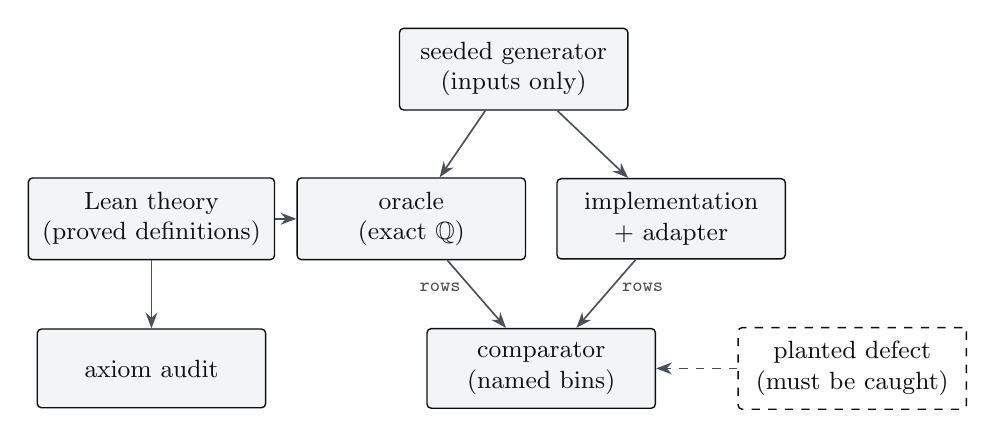
\begin{tikzpicture}[
  box/.style={draw=Ink, line width=0.5pt, fill=Surface, text=Ink, rounded corners=1.5pt,
    align=center, font=\small, inner sep=5pt, minimum height=10mm, minimum width=29mm},
  arr/.style={-{Stealth[length=2mm]}, line width=0.6pt, draw=InkMuted},
  lab/.style={font=\ttfamily\scriptsize, text=InkMuted}]
\node[box] (gen) at (4.6,1.9) {seeded generator\\(inputs only)};
\node[box] (theory) at (0,0) {Lean theory\\(proved definitions)};
\node[box] (oracle) at (3.3,0) {oracle\\(exact $\mathbb{Q}$)};
\node[box] (impl) at (6.6,0) {implementation\\+ adapter};
\node[box] (cmp) at (4.95,-1.9) {comparator\\(named bins)};
\node[box] (audit) at (0,-1.9) {axiom audit};
\node[box, dashed, fill=Background] (planted) at (8.9,-1.9) {planted defect\\(must be caught)};
\draw[arr] (gen) -- (oracle);
\draw[arr] (gen) -- (impl);
\draw[arr] (theory) -- (oracle);
\draw[arr] (theory) -- (audit);
\draw[arr] (oracle) -- node[left, lab, pos=0.4] {rows} (cmp);
\draw[arr] (impl) -- node[right, lab, pos=0.4] {rows} (cmp);
\draw[arr, dashed] (planted) -- (cmp);
\end{tikzpicture}
\caption{The measurement procedure. The generator never computes expected results;
those come only from the oracle.}
\label{fig:harness}
\end{figure}

The procedure follows \texttt{ledger-semantics} (\cref{fig:harness}). A seeded
generator writes case files containing inputs only. It favors the inputs where
implementations are known to have conventions: tied logits, words that are
themselves tokens, and merge tables with several splits of one string. A small
adapter per implementation runs the same cases and prints the oracle's row format.
The comparator places every case in exactly one named bin (agree, diverge, skipped
by either side, or missing), so nothing is dropped silently. Token rows are compared
as strings. Sampler rows require that a zero be matched by a zero and that nonzero
probabilities agree within $10^{-6}$, since llama.cpp stores logits in
\texttt{float32}. Each comparator is observed to fail: a planted defect, an adapter
that glues two tokens or one that inverts temperature, must be detected or the run
fails.

\paragraph{Tie divergences.} An implementation that keeps exactly $k$ tokens breaks
ties in its own order, which need not be the oracle's order by index. Every filter
treats tied tokens alike except for that choice, and tied tokens stay tied through
temperature and renormalization. Such an implementation must therefore agree with
the positional semantics up to a permutation of tied tokens. The harness checks
exactly this: the multiset of (logit, probability) pairs over the kept tokens must
equal that of the oracle's \texttt{q} rows. A divergence that fails this check is
reported as unexplained.

\begin{table}[t]
\centering\small
\caption{Measurements (\texttt{harness/run.sh 600}: four seeds of 600 cases each per
corpus). Lean 4.34.1, Mathlib v4.34.1, \texttt{tokenizers} 0.23.3, \texttt{tiktoken}
0.14.0, llama.cpp commit \texttt{a9d27ac} (2026-10-11).}
\label{tab:results}
\begin{tabularx}{\linewidth}{@{}>{\raggedright\arraybackslash}p{4.6cm}>{\raggedright\arraybackslash}X>{\raggedright\arraybackslash}X@{}}
\toprule
\qpth{Implementation} & \qpth{Compared against} & \qpth{Result}\\
\midrule
HF \texttt{tokenizers}, BPE, defaults & rule-rank BPE (\lean{bpe}) & 13{,}779 / 13{,}779 words identical\\
HF \texttt{tokenizers}, \lean{ignore_merges} & lookup, then rule-rank BPE & 13{,}779 / 13{,}779 identical\\
\texttt{tiktoken} & lookup, then concatenation-rank BPE & 13{,}779 / 13{,}779 identical\\
llama.cpp \lean{top_k}, \lean{top_p}, \lean{min_p}, \texttt{temp}, no ties & tie-keeping filters & 1{,}216 / 1{,}216 chains, $|\Delta p|\le5.1\times10^{-8}$\\
llama.cpp, with ties & tie-keeping, else positional & 939 + 245 / 1{,}184 chains; 0 unexplained\\
Planted defects (tokenizer, sampler) & --- & both detected\\
\bottomrule
\end{tabularx}
\end{table}

\Cref{tab:results} summarizes the results. Two findings came out of the
comparisons. First, \texttt{tiktoken} initially disagreed with the oracle's
concatenation-rank BPE on words that are themselves vocabulary tokens. The
disagreement was a convention, whole-word lookup. Following the
\texttt{ledger-semantics} rule that a divergence is either a defect in the
implementation or a convention the semantics has not yet recorded, we recorded it
as \lean{lookupFirst}, with its own theorems, after which agreement is exact.
Second, on the same random merge tables the two tokenizer libraries disagree with
each other on 439 of 13{,}779 words (3.2\%), and on 279 when Hugging Face uses
\lean{ignore_merges}. The oracle reproduces each library exactly, so every one of
these disagreements is predicted. \Cref{thm:bpeconv} states the condition under which
they cannot occur.

For sampling, llama.cpp agrees with the tie-keeping semantics on every tie-free
chain. On chains with ties, 245 of 1{,}184 diverge, and every one agrees with the
positional semantics up to a permutation of tied tokens. Some of these divergences
cascade: a tie cut by top-$k$ changes the renormalized masses that a later top-$p$
sees. A check that compared kept sets only after the fact would misclassify such
cases. Replaying the convention exactly classifies all of them.

% ===========================================================================
\section{Related work}

\paragraph{Formal methods for machine learning.} Most verification work on neural
networks proves properties of trained models, for example with SMT-based
methods~\cite{katz2017reluplex}. We verify the model-independent algorithms around
the model instead, and connect them to implementations through an oracle. The
denotational method follows Elliott~\cite{elliott2009denotational}. The use of a
proved semantics as a test oracle, the procedure of planted defects, and the
discipline of named skip bins follow \texttt{ledger-semantics}~\cite{ledgersemantics}.
Our category of finite stochastic maps is a special case of Fritz's Markov
categories~\cite{fritz2020markov}.

\paragraph{Tokenization.} Zouhar et al.\ give a formal analysis of BPE as an
optimization problem~\cite{zouhar2023bpe}. Gastaldi et al.\ treat tokenizers as
stochastic maps and study consistency of estimators~\cite{gastaldi2024foundations}.
Vieira et al.\ show how to turn token-level models into character-level
ones~\cite{vieira2024tokens}, which requires exactly the enumeration of
tokenizations we verify. Our no-compression theorem and the agreement criterion
between BPE conventions complement this work at the level of exact identities.

\paragraph{Decoding.} Top-$k$~\cite{fan2018hierarchical}, nucleus~\cite{holtzman2020curious}
and min-$p$~\cite{nguyen2025minp} sampling are usually specified by an algorithm over
sorted arrays, which leaves ties unspecified. \Cref{thm:topk} shows that this gap
cannot be closed by any symmetric rule. Speculative
sampling~\cite{leviathan2023speculative,chen2023speculative} is known to be lossless,
and its acceptance rate is the maximal-coupling bound~\cite{lindvall1992coupling}. Du et
al.\ characterize tightness measure-theoretically~\cite{du2023tight}. We give a
finite-depth statement and an explicit non-tight model.

\paragraph{Attention and inference systems.} Online softmax~\cite{milakov2018online}
underlies FlashAttention~\cite{dao2022flashattention} and its successors, and
KV caching is standard in serving systems~\cite{pope2023scaling,kwon2023vllm}. Our
contribution is the algebraic packaging, a commutative monoid with a free-monoid
homomorphism, and machine-checked proofs over arbitrary exponential characters.
Permutation equivariance of attention without positional encodings is
known~\cite{yun2020universal}.

\paragraph{Masked diffusion.} The time-independence of the optimal denoiser was
observed by Ou et al.~\cite{ou2025absorbing}, in the setting of
D3PM~\cite{austin2021d3pm}, MDLM~\cite{sahoo2024mdlm} and related
models~\cite{shi2024masked,nie2025llada}. We machine-check it, together with the
any-order chain rule and the inexactness of parallel unmasking.

% ===========================================================================
\section{Limitations}

Analysis on the reals enters only through exponential characters, and there is no
measure theory, so sampling and tightness are stated through finite quantities. The
oracle's temperature is restricted to $1/n$, which keeps softmax rational. The
theorems hold for every temperature, but the oracle cannot evaluate an irrational
softmax. Speculative decoding is proved for one drafted token. The sequence version
follows by induction and is not yet formalized. Nothing is proved about
floating-point arithmetic: implementations are compared with exact values within a
stated tolerance. A decision that lies exactly on a floating-point boundary could in
principle diverge, and none occurred in our runs. The diffusion theory covers
absorbing diffusion, not Gaussian diffusion. The chat protocol models tool calling in
its common request-and-result form, not any vendor's specification. The measurements
cover tokenizers and samplers; attention kernels, speculative decoders, chat
renderers and diffusion samplers are evaluated by the oracle but not yet compared
against implementations.

% ===========================================================================
\section{Conclusion}

The inference side of LLMs is small enough to be given a precise meaning and large
enough that its implementations disagree. A machine-checked semantics separates
what is meaning from what is convention. It proves which reorderings, cachings and
tilings are harmless, and it shows that some properties folklore expects, such as
symmetric exact top-$k$, compositional compressing tokenizers and unambiguous plain-text
templates, cannot exist. Connected to an exact oracle, the same definitions become
a test instrument. Every divergence it surfaces is either a defect in an
implementation or a convention that belongs in the semantics.

\paragraph{Availability.} The Lean development, oracle, harness, and recorded
measurement log accompany this paper.

\paragraph{Acknowledgments.} The structure of this work follows
\texttt{ledger-semantics} by John Wiegley. The formalization and harness were
developed with the assistance of an AI system (Claude, Anthropic).

% ===========================================================================
\begin{thebibliography}{99}\small

\bibitem{austin2021d3pm}
J.~Austin, D.~D. Johnson, J.~Ho, D.~Tarlow, and R.~van~den Berg.
\newblock Structured denoising diffusion models in discrete state-spaces.
\newblock In \emph{NeurIPS}, 2021.

\bibitem{chen2023speculative}
C.~Chen, S.~Borgeaud, G.~Irving, J.-B. Lespiau, L.~Sifre, and J.~Jumper.
\newblock Accelerating large language model decoding with speculative sampling.
\newblock arXiv:2302.01318, 2023.

\bibitem{dao2022flashattention}
T.~Dao, D.~Y. Fu, S.~Ermon, A.~Rudra, and C.~R{\'e}.
\newblock {FlashAttention}: Fast and memory-efficient exact attention with {IO}-awareness.
\newblock In \emph{NeurIPS}, 2022.

\bibitem{demoura2021lean4}
L.~de~Moura and S.~Ullrich.
\newblock The {Lean} 4 theorem prover and programming language.
\newblock In \emph{CADE-28}, 2021.

\bibitem{du2023tight}
L.~Du, L.~Torroba~Hennigen, T.~Pimentel, C.~Meister, J.~Eisner, and R.~Cotterell.
\newblock A measure-theoretic characterization of tight language models.
\newblock In \emph{ACL}, 2023.

\bibitem{elliott2009denotational}
C.~Elliott.
\newblock Denotational design with type class morphisms.
\newblock Technical Report 2009-01, LambdaPix, 2009.

\bibitem{fan2018hierarchical}
A.~Fan, M.~Lewis, and Y.~Dauphin.
\newblock Hierarchical neural story generation.
\newblock In \emph{ACL}, 2018.

\bibitem{fritz2020markov}
T.~Fritz.
\newblock A synthetic approach to {Markov} kernels, conditional independence and theorems on sufficient statistics.
\newblock \emph{Advances in Mathematics}, 370, 2020.

\bibitem{gastaldi2024foundations}
J.~L. Gastaldi, J.~Terilla, L.~Malagutti, B.~DuSell, T.~Vieira, and R.~Cotterell.
\newblock The foundations of tokenization: Statistical and computational concerns.
\newblock arXiv:2407.11606, 2024.

\bibitem{greshake2023injection}
K.~Greshake, S.~Abdelnabi, S.~Mishra, C.~Endres, T.~Holz, and M.~Fritz.
\newblock Not what you've signed up for: Compromising real-world {LLM}-integrated applications with indirect prompt injection.
\newblock In \emph{AISec}, 2023.

\bibitem{holtzman2020curious}
A.~Holtzman, J.~Buys, L.~Du, M.~Forbes, and Y.~Choi.
\newblock The curious case of neural text degeneration.
\newblock In \emph{ICLR}, 2020.

\bibitem{katz2017reluplex}
G.~Katz, C.~Barrett, D.~L. Dill, K.~Julian, and M.~J. Kochenderfer.
\newblock Reluplex: An efficient {SMT} solver for verifying deep neural networks.
\newblock In \emph{CAV}, 2017.

\bibitem{kwon2023vllm}
W.~Kwon, Z.~Li, S.~Zhuang, Y.~Sheng, L.~Zheng, C.~H. Yu, J.~E. Gonzalez, H.~Zhang, and I.~Stoica.
\newblock Efficient memory management for large language model serving with {PagedAttention}.
\newblock In \emph{SOSP}, 2023.

\bibitem{ledgersemantics}
J.~Wiegley.
\newblock ledger-semantics: Mathematical semantics of {Ledger}, the double-entry accounting tool.
\newblock \url{https://github.com/ledger/ledger-semantics}, 2026.

\bibitem{leviathan2023speculative}
Y.~Leviathan, M.~Kalman, and Y.~Matias.
\newblock Fast inference from transformers via speculative decoding.
\newblock In \emph{ICML}, 2023.

\bibitem{lindvall1992coupling}
T.~Lindvall.
\newblock \emph{Lectures on the Coupling Method}.
\newblock Wiley, 1992.

\bibitem{liu2023ring}
H.~Liu, M.~Zaharia, and P.~Abbeel.
\newblock Ring attention with blockwise transformers for near-infinite context.
\newblock arXiv:2310.01889, 2023.

\bibitem{mathlib2020}
The mathlib Community.
\newblock The {Lean} mathematical library.
\newblock In \emph{CPP}, 2020.

\bibitem{milakov2018online}
M.~Milakov and N.~Gimelshein.
\newblock Online normalizer calculation for softmax.
\newblock arXiv:1805.02867, 2018.

\bibitem{nguyen2025minp}
M.~N. Nguyen, A.~Baker, C.~Neo, A.~Roush, A.~Kirsch, and R.~Shwartz-Ziv.
\newblock Turning up the heat: Min-p sampling for creative and coherent {LLM} outputs.
\newblock In \emph{ICLR}, 2025.

\bibitem{nie2025llada}
S.~Nie, F.~Zhu, Z.~You, X.~Zhang, J.~Ou, J.~Hu, J.~Zhou, Y.~Lin, J.-R. Wen, and C.~Li.
\newblock Large language diffusion models.
\newblock arXiv:2502.09992, 2025.

\bibitem{ou2025absorbing}
J.~Ou, S.~Nie, K.~Xue, F.~Zhu, J.~Sun, Z.~Li, and C.~Li.
\newblock Your absorbing discrete diffusion secretly models the conditional distributions of clean data.
\newblock In \emph{ICLR}, 2025.

\bibitem{pope2023scaling}
R.~Pope, S.~Douglas, A.~Chowdhery, J.~Devlin, J.~Bradbury, J.~Heek, K.~Xiao, S.~Agrawal, and J.~Dean.
\newblock Efficiently scaling transformer inference.
\newblock In \emph{MLSys}, 2023.

\bibitem{rabe2021selfattention}
M.~N. Rabe and C.~Staats.
\newblock Self-attention does not need {$O(n^2)$} memory.
\newblock arXiv:2112.05682, 2021.

\bibitem{radford2019gpt2}
A.~Radford, J.~Wu, R.~Child, D.~Luan, D.~Amodei, and I.~Sutskever.
\newblock Language models are unsupervised multitask learners.
\newblock OpenAI technical report, 2019.

\bibitem{sahoo2024mdlm}
S.~S. Sahoo, M.~Arriola, Y.~Schiff, A.~Gokaslan, E.~Marroquin, J.~T. Chiu, A.~Rush, and V.~Kuleshov.
\newblock Simple and effective masked diffusion language models.
\newblock In \emph{NeurIPS}, 2024.

\bibitem{sennrich2016bpe}
R.~Sennrich, B.~Haddow, and A.~Birch.
\newblock Neural machine translation of rare words with subword units.
\newblock In \emph{ACL}, 2016.

\bibitem{shi2024masked}
J.~Shi, K.~Han, Z.~Wang, A.~Doucet, and M.~K. Titsias.
\newblock Simplified and generalized masked diffusion for discrete data.
\newblock In \emph{NeurIPS}, 2024.

\bibitem{vieira2024tokens}
T.~Vieira, B.~LeBrun, M.~Giulianelli, J.~L. Gastaldi, B.~DuSell, J.~Terilla, T.~J. O'Donnell, and R.~Cotterell.
\newblock From language models over tokens to language models over characters.
\newblock arXiv:2412.03719, 2024.

\bibitem{wolf2020transformers}
T.~Wolf et~al.
\newblock Transformers: State-of-the-art natural language processing.
\newblock In \emph{EMNLP: System Demonstrations}, 2020.

\bibitem{xiao2024sinks}
G.~Xiao, Y.~Tian, B.~Chen, S.~Han, and M.~Lewis.
\newblock Efficient streaming language models with attention sinks.
\newblock In \emph{ICLR}, 2024.

\bibitem{yun2020universal}
C.~Yun, S.~Bhojanapalli, A.~S. Rawat, S.~J. Reddi, and S.~Kumar.
\newblock Are transformers universal approximators of sequence-to-sequence functions?
\newblock In \emph{ICLR}, 2020.

\bibitem{zouhar2023bpe}
V.~Zouhar, C.~Meister, J.~L. Gastaldi, L.~Du, T.~Vieira, M.~Sachan, and R.~Cotterell.
\newblock A formal perspective on byte-pair encoding.
\newblock In \emph{Findings of ACL}, 2023.

\end{thebibliography}

\end{document}
"

\usepackage[a4paper,textwidth=15.4cm,textheight=23.6cm,top=3.0cm,headsep=0.9cm,footskip=1.2cm]{geometry}
\usepackage{amsmath,amssymb,amsthm,mathtools}
\usepackage{fontspec}
\usepackage{booktabs,tabularx,array}
\usepackage[protrusion=true,expansion=false]{microtype}
\usepackage[table]{xcolor}
\usepackage{graphicx}
\usepackage{fvextra}
\usepackage{enumitem}
\usepackage{caption}
\usepackage{titlesec}
\usepackage{fancyhdr}
\usepackage[most]{tcolorbox}
\usepackage{tikz}
\usetikzlibrary{arrows.meta}
\usepackage{hyperref}
\usepackage[nameinlink,capitalise]{cleveref}

% ---------------------------------------------------------------------------
%  Colour tokens
% ---------------------------------------------------------------------------
% Neutral foundation. Ink and Background invert between the two editions.
\ifqptdark
  \definecolor{Background}{HTML}{0B0C0E}
  \definecolor{Surface}{HTML}{16181B}
  \definecolor{Border}{HTML}{2B2E33}
  \definecolor{Ink}{HTML}{EDEEF0}
  \definecolor{InkMuted}{HTML}{A9AEB6}
  \definecolor{InkFaint}{HTML}{5A5F67}   % decoration only, never meaningful text
\else
  \definecolor{Background}{HTML}{FFFFFF}
  \definecolor{Surface}{HTML}{F3F4F5}
  \definecolor{Border}{HTML}{DADDE1}
  \definecolor{Ink}{HTML}{0E0F11}
  \definecolor{InkMuted}{HTML}{4B4F57}
  \definecolor{InkFaint}{HTML}{A3A7AE}   % decoration only, never meaningful text
\fi
% Paradigm colours: fixed in both editions, semantic only.
\definecolor{Quantum}{HTML}{5BAD1E}
\definecolor{Photonic}{HTML}{F0AB00}
\definecolor{Thermodynamic}{HTML}{E8690A}
\definecolor{Ternary}{HTML}{8A8A8A}
\definecolor{Bio}{HTML}{1AAB7C}

\ifqptdark\pagecolor{Background}\fi

% ---------------------------------------------------------------------------
%  Typography
% ---------------------------------------------------------------------------
\setmainfont{Inter}[
  Path=fonts/, Extension=.otf, Scale=0.94,
  UprightFont=*-Regular, ItalicFont=*-Italic,
  BoldFont=*-SemiBold, BoldItalicFont=*-SemiBoldItalic]
\setmonofont{IBMPlexMono}[
  Path=fonts/, Extension=.ttf, Scale=MatchLowercase,
  UprightFont=*-Regular, ItalicFont=*-Italic, BoldFont=*-SemiBold]
\newfontfamily\qptdisplay{SpaceGrotesk}[
  Path=fonts/, Extension=.otf, UprightFont=*-Medium, BoldFont=*-Bold]
\newfontfamily\qptdisplaylight{SpaceGrotesk}[
  Path=fonts/, Extension=.otf, UprightFont=*-Regular]
\newfontfamily\qptlabelfont{IBMPlexMono}[
  Path=fonts/, Extension=.ttf, Scale=MatchLowercase, UprightFont=*-Medium,
  LetterSpace=6]
\setsansfont{Inter}[
  Path=fonts/, Extension=.otf, Scale=0.94,
  UprightFont=*-Regular, ItalicFont=*-Italic,
  BoldFont=*-SemiBold, BoldItalicFont=*-SemiBoldItalic]
\linespread{1.16}
\setlength{\emergencystretch}{2.5em}
\AtBeginDocument{\raggedright\setlength{\parindent}{0pt}}
\setlength{\parindent}{0pt}
\setlength{\parskip}{0.55em}

% A label: IBM Plex Mono, upper case, tracked.
\newcommand{\qptlabel}[1]{{\qptlabelfont\footnotesize\MakeUppercase{#1}}}
% Technical names (Lean declarations, files) in IBM Plex Mono.
\newcommand{\lean}[1]{\texttt{\detokenize{#1}}}
\newcommand{\leanref}[1]{\par\smallskip\noindent
  {\ttfamily\footnotesize\upshape\raggedright\color{InkMuted}LEAN\enspace #1\par}}

% Ink is the normal colour everywhere, including floats, heads and footnotes.
\makeatletter
\AtBeginDocument{\color{Ink}\global\let\default@color\current@color}
\makeatother

% ---------------------------------------------------------------------------
%  Mathematical notation
% ---------------------------------------------------------------------------
\newcommand{\K}{\Bbbk}
\newcommand{\Dist}{\mathrm{Dist}}
\newcommand{\restr}[2]{#1|_{#2}}
\newcommand{\topk}{\mathrm{TopK}}
\newcommand{\topp}{\mathrm{TopP}}
\newcommand{\minp}{\mathrm{MinP}}
\newcommand{\sharpen}{\mathrm{sharpen}}
\newcommand{\abv}{\mathrm{above}}
\newcommand{\tv}{\mathrm{tv}}
\newcommand{\dec}{\mathrm{dec}}
\newcommand{\enc}{\mathrm{enc}}
\newcommand{\softmax}{\mathrm{softmax}}
\newcommand{\attend}{\mathrm{attend}}
\newcommand{\Iv}[1]{[\![#1]\!]}
\newcommand{\Mask}{\bot}

% ---------------------------------------------------------------------------
%  Headings: section numbers as labels, titles in Space Grotesk
% ---------------------------------------------------------------------------
\makeatletter
\newcommand{\qptsecnum}[1]{{\qptlabelfont\small\color{InkMuted}\two@digits{#1}}}
\makeatother
\titleformat{\section}
  {\qptdisplay\fontsize{14.5}{18}\selectfont\color{Ink}}
  {\qptsecnum{\value{section}}}{0.9em}{}
\titleformat{name=\section,numberless}
  {\qptdisplay\fontsize{14.5}{18}\selectfont\color{Ink}}{}{0pt}{}
\titlespacing*{\section}{0pt}{1.9em}{0.7em}
\titleformat{\paragraph}[runin]
  {\qptdisplay\normalsize\color{Ink}}{}{0pt}{}
\titlespacing*{\paragraph}{0pt}{0.9em}{0.6em}

% ---------------------------------------------------------------------------
%  Statements
% ---------------------------------------------------------------------------
\newtheoremstyle{qpt}
  {0.9em}{0.9em}
  {\normalfont}{}
  {\qptlabelfont\footnotesize}{}
  {\newline}
  {\MakeUppercase{\thmname{#1}\thmnumber{~#2}}%
   \thmnote{\enspace{\qptdisplay\normalsize\color{Ink}#3}}}
\theoremstyle{qpt}
\newtheorem{theorem}{Theorem}
\newtheorem{proposition}[theorem]{Proposition}
\newtheorem{corollary}[theorem]{Corollary}
\newtheorem{lemma}[theorem]{Lemma}
\newtheorem{definition}[theorem]{Definition}
\newtheorem{remark}[theorem]{Remark}

% Proofs: a tracked label and a neutral end mark.
\makeatletter
\renewcommand{\qedsymbol}{{\color{InkMuted}\rule{0.5em}{0.5em}}}
\renewenvironment{proof}[1][Proof]{\par\pushQED{\qed}\normalfont\topsep0.5em\relax
  \trivlist\item[\hskip\labelsep\qptlabel{#1}\hspace{0.6em}]\ignorespaces}
  {\popQED\endtrivlist\@endpefalse}
\makeatother

% ---------------------------------------------------------------------------
%  Code: IBM Plex Mono on a neutral surface, with a hairline on the left
% ---------------------------------------------------------------------------
\tcbset{colupper=Ink, collower=Ink}
\tcbset{qptcode/.style={enhanced, colback=Surface, colframe=Surface,
  boxrule=0pt, arc=0pt, left=9pt, right=8pt, top=5pt, bottom=5pt,
  borderline west={1.2pt}{0pt}{InkFaint}, before skip=0.7em, after skip=0.7em}}
\newenvironment{leancode}
  {\VerbatimEnvironment\begin{tcolorbox}[qptcode]%
   \begin{Verbatim}[fontsize=\small,commandchars=\\\{\},
     codes={\catcode`\$=3\catcode`\^=7},formatcom=\color{Ink}]}
  {\end{Verbatim}\end{tcolorbox}}
\newenvironment{casecode}
  {\VerbatimEnvironment\begin{tcolorbox}[qptcode,before skip=0pt,after skip=0pt]%
   \begin{Verbatim}[fontsize=\footnotesize,formatcom=\color{Ink}]}
  {\end{Verbatim}\end{tcolorbox}}

% ---------------------------------------------------------------------------
%  Floats, tables, captions
% ---------------------------------------------------------------------------
\DeclareCaptionLabelFormat{qpt}{\qptlabel{#1~#2}}
\DeclareCaptionLabelSeparator{qptsep}{\quad}
\captionsetup{labelformat=qpt, labelsep=qptsep, font={small,color=Ink},
  justification=raggedright, singlelinecheck=false, skip=6pt}
\newcommand{\qpth}[1]{\qptlabel{#1}}
\arrayrulecolor{Ink}
\setlength{\heavyrulewidth}{0.7pt}
\setlength{\lightrulewidth}{0.35pt}
\renewcommand{\arraystretch}{1.22}

% ---------------------------------------------------------------------------
%  Running heads
% ---------------------------------------------------------------------------
\pagestyle{fancy}
\fancyhf{}
\fancyhead[L]{{\color{Ink}\qptlabel{Machine-checked semantics of LLM inference}}}
\fancyhead[R]{{\color{Ink}\qptlabel{D. Arango Sohm}}}
\fancyfoot[R]{{\ttfamily\small\color{InkMuted}\thepage}}
\renewcommand{\headrule}{{\color{Border}\hrule height 0.4pt}\vspace{-0.4pt}}
\renewcommand{\headrulewidth}{0.4pt}
\fancypagestyle{qptfirst}{\fancyhf{}%
  \fancyfoot[R]{{\ttfamily\small\color{InkMuted}\thepage}}%
  \renewcommand{\headrulewidth}{0pt}\renewcommand{\headrule}{}}

% ---------------------------------------------------------------------------
%  Links and references: neutral, never accent-coloured text
% ---------------------------------------------------------------------------
\hypersetup{colorlinks=true, linkcolor=Ink, citecolor=Ink, urlcolor=Ink,
  pdftitle={A Machine-Checked Semantics of LLM Inference},
  pdfauthor={Daniel Arango Sohm},
  pdfsubject={Formal semantics of large language model inference in Lean 4},
  pdfkeywords={Lean 4, Mathlib, formal verification, LLM inference, sampling,
    tokenization, attention, speculative decoding, diffusion language models}}
\makeatletter
\renewcommand{\@biblabel}[1]{{\ttfamily\color{InkMuted}[#1]}}
\renewcommand{\@cite}[2]{{\ttfamily[#1\if@tempswa, #2\fi]}}
\makeatother
\renewcommand{\refname}{References}

\setlist{itemsep=2pt, topsep=4pt}
\setlist[itemize]{label={\color{InkMuted}\textbullet}}

\begin{document}
\thispagestyle{qptfirst}

% ----------------------------------------------------------------- masthead
\noindent
\begin{minipage}[c]{0.5\linewidth}
  \includegraphics[height=1.9cm]{qpt-logo.png}
\end{minipage}%
\begin{minipage}[c]{0.5\linewidth}\raggedleft
  \qptlabel{Preprint}\\[2pt]
  \qptlabel{October 2026}
\end{minipage}

\vspace{1.6em}
{\color{Border}\rule{\linewidth}{0.4pt}}
\vspace{1.1em}

{\qptdisplay\fontsize{25}{29.5}\selectfont\color{Ink}
A Machine-Checked Semantics\\ of LLM Inference\par}
\vspace{0.55em}
{\qptdisplaylight\fontsize{13}{17}\selectfont\color{InkMuted}
Sampling, Attention, Tokenization, Chat, Decoding,\\ and Diffusion in Lean~4\par}

\vspace{1.5em}
{\large\bfseries Daniel Arango Sohm}\par
\vspace{0.15em}
{\color{InkMuted}Universidad EAFIT, Medellín, Colombia\\
Former member of the QPT team}\par

\vspace{1.4em}
% ----------------------------------------------------------------- abstract
\begin{tcolorbox}[enhanced, colback=Surface, colframe=Surface, colupper=Ink, boxrule=0pt,
  arc=0pt, left=12pt, right=12pt, top=9pt, bottom=10pt]
\qptlabel{Abstract}\par\vspace{0.35em}
{\small
The inference side of a large language model is a stack of small algorithms:
tokenizers, attention kernels, key--value caches, sampling filters, speculative
decoders, chat templates, and diffusion samplers. Each has several independent
implementations, and those implementations are usually tested against one another
rather than against a definition. We give these components a single mathematical
semantics, formalized in Lean~4 against Mathlib. The development comprises about
4{,}600 lines and 270 named theorems, and every declaration depends only on Lean's
three standard axioms. It proves the exact algebra of sampling filters, the
losslessness and optimality of speculative sampling, and the correctness of
key--value caching and of FlashAttention-style online softmax as a commutative
monoid. It proves that byte-pair encoding is lossless under every merge priority,
together with a decidable criterion for when the Hugging Face and \texttt{tiktoken}
conventions agree, a protocol checker for tool calls, and the time-independence of
the masked-diffusion denoiser. It also proves six negative results. No sampling
rule that treats tokens symmetrically can always keep exactly $k$ tokens. No
tokenizer that compresses can respect concatenation. Every chat template that writes
its role markers in the content alphabet is ambiguous. No transformer without
positional information can copy a fixed position. An autoregressive model need not
define a distribution over strings. Parallel unmasking in diffusion is inexact.
From the same definitions we build an executable oracle that evaluates test cases in
exact rational arithmetic, and a harness that measures implementations against it.
On 2{,}400 random merge tables, Hugging Face \texttt{tokenizers} and
\texttt{tiktoken} each agree with the oracle on all 13{,}779 test words, while
disagreeing with each other on 3.2\% of them. On 2{,}400 random sampler chains,
every divergence of llama.cpp from the tie-keeping semantics is accounted for
exactly by the positional semantics that the impossibility theorem forces.
\par}
\end{tcolorbox}

\vspace{0.3em}
\noindent\qptlabel{Keywords}\enspace{\small Lean~4 · Mathlib · formal verification ·
LLM inference · sampling · tokenization · attention · speculative decoding ·
diffusion language models}

\vspace{0.4em}
{\color{Border}\rule{\linewidth}{0.4pt}}

% ===========================================================================
\section{Introduction}

A deployed language model is a function from parameters and a context to a
distribution over tokens. Turning that distribution into text requires more
machinery. A tokenizer maps strings to token sequences. Attention kernels compute
the model's reads over a cached context. A chain of sampling filters reshapes the
next-token distribution. A speculative decoder may verify drafted tokens, a chat
template linearizes a conversation, and a diffusion sampler may unmask several
positions at once. Each of these components exists in many implementations, such as
Hugging Face \texttt{transformers} and \texttt{tokenizers}~\cite{wolf2020transformers},
\texttt{tiktoken}, vLLM~\cite{kwon2023vllm}, and llama.cpp. Their tests mostly
compare one implementation with another, or with remembered behavior.

This paper follows a different discipline, \emph{denotational design}~\cite{elliott2009denotational}.
One first says precisely what a thing means, then requires every operation to
preserve that meaning, and lets the implementation be whatever the equations force
it to be. The approach is that of \texttt{ledger-semantics}~\cite{ledgersemantics},
which formalizes double-entry accounting in Lean and uses the result as a test oracle
for the C++ Ledger program. We apply it to LLM inference. A sampling filter means
conditioning a distribution on a set. A KV-cached decoder means causal attention over
the whole prefix. A FlashAttention kernel means a softmax-weighted average. A chat
template means an injective encoding of a transcript. The theorems state when an
implementation preserves that meaning, and several of them state that no
implementation can.

\paragraph{Contributions.}
\begin{itemize}[leftmargin=*,itemsep=2pt]
\item A Lean~4 formalization against Mathlib~\cite{mathlib2020,demoura2021lean4}
  of sampling, speculative decoding, softmax and attention, tokenization, chat
  transcripts, autoregressive decoding, and masked diffusion
  (\cref{sec:foundations,sec:sampling,sec:spec,sec:attention,sec:tokenization,sec:chat,sec:decoding,sec:diffusion}).
  All definitions are stated over an arbitrary linearly ordered field, so one proof
  covers the real numbers of the literature and the exact rationals of the oracle.
\item Positive results in a common framework. They include the algebra of
  sampling filters, the optimality of speculative sampling, an online-softmax
  commutative monoid, a generic correctness theorem for BPE with a decidable
  agreement criterion between the two conventions in use, a protocol checker for
  tool calls, and the any-order chain rule for masked diffusion.
\item Six negative results that explain design constraints visible across
  implementations (\cref{sec:negative}).
\item An executable oracle that evaluates case files under the proved
  definitions in exact arithmetic, and a measurement of Hugging Face
  \texttt{tokenizers}, \texttt{tiktoken}, and llama.cpp against it (\cref{sec:oracle,sec:measure}).
\end{itemize}

Several of the positive results are known: losslessness of speculative
sampling~\cite{leviathan2023speculative,chen2023speculative}, correctness of online
softmax~\cite{milakov2018online,dao2022flashattention}, time-independence of the
absorbing-diffusion posterior~\cite{ou2025absorbing}, and the role of permutation
equivariance~\cite{yun2020universal}. Our contribution for these is a machine-checked
statement in one framework, connected to an oracle. To our knowledge the
following are not stated elsewhere in the form given here: the impossibility of
symmetric exact top-$k$ and nucleus selection, the no-compression theorem for
homomorphic tokenizers, the ambiguity of every in-band chat template, and the
decidable agreement criterion between merge-rule and concatenation-rank BPE.

% ===========================================================================
\section{Method and trust base}\label{sec:method}

The development is a Lean~4 library (Lean 4.34.1, Mathlib v4.34.1) of eleven
theory modules and two executable modules (\cref{tab:modules}). It is built with
warnings promoted to errors, so an unproved theorem (\lean{sorry}) fails the build.
A separate audit program walks every declaration in the library, 853 in all, and
fails unless each depends only on propositional extensionality, the axiom of choice,
and quotient soundness. The audit has been observed to fail: a planted proof by
\lean{native_decide}, which introduces an auxiliary axiom trusting compiled code, is
rejected. The warnings-as-errors build alone does not catch it. Concrete
counterexamples are therefore proved by \lean{decide}, whose certificate the kernel
checks by evaluation.

\begin{table}[t]
\centering\small
\caption{Modules of the development. Lines and named theorems and lemmas per module.}
\label{tab:modules}
\begin{tabularx}{\linewidth}{@{}l>{\raggedright\arraybackslash}X>{\ttfamily}r>{\ttfamily}r@{}}
\toprule
\qpth{Module} & \qpth{Content} & \qpth{Lines} & \qpth{Thms} \\
\midrule
\lean{Dist} & finite distributions, conditioning, total variation, $\mathsf{FinStoch}$ & 383 & 34\\
\lean{Sampling} & top-$k$, top-$p$, min-$p$, temperature, ties, inverse CDF & 732 & 46\\
\lean{Counterexamples} & kernel-checked failures of sampler laws & 52 & 4\\
\lean{Speculative} & speculative sampling, couplings & 194 & 17\\
\lean{Softmax} & exponential characters, masking, temperature & 220 & 23\\
\lean{Attention} & equivariance, causality, KV cache, online softmax & 573 & 38\\
\lean{Real} & $\exp$ as a character; textbook restatements & 51 & 4\\
\lean{Tokenization} & free-monoid decoding, BPE conventions, enumeration & 860 & 49\\
\lean{Chat} & tool-call protocol, rendering & 440 & 21\\
\lean{Decoding} & mass conservation, tightness, greedy decoding & 245 & 15\\
\lean{Diffusion} & masked diffusion, posterior, chain rule & 379 & 18\\
\lean{Oracle}, \lean{Driver} & case parsing and exact evaluation & 465 & 1\\
\midrule
Total & & 4{,}594 & 270\\
\bottomrule
\end{tabularx}
\end{table}

\paragraph{Numbers.} Every probability lives in an arbitrary field $\K$ with a
compatible linear order (\lean{[Field K] [LinearOrder K] [IsStrictOrderedRing K]}).
The oracle instantiates $\K=\mathbb{Q}$, so its arithmetic is exact. The analytic
statements instantiate $\K=\mathbb{R}$. No measure theory is used. Sampling is made
precise through interval statements (\cref{thm:invcdf}), and tightness through
masses at finite depth (\cref{sec:decoding}).

% ===========================================================================
\section{Foundations}\label{sec:foundations}

\begin{definition}[Finite distribution]
For a finite type $\alpha$, $\Dist_\K(\alpha)$ is the type of functions
$p:\alpha\to\K$ with $p(a)\ge 0$ for all $a$ and $\sum_a p(a)=1$.
\leanref{\lean{Dist}}
\end{definition}

\begin{leancode}
structure Dist ($\K$ : Type u) [Field $\K$] [LinearOrder $\K$] [IsStrictOrderedRing $\K$]
    ($\alpha$ : Type v) [Fintype $\alpha$] where
  prob : $\alpha$ $\to$ $\K$
  nonneg : $\forall$ a, 0 $\le$ prob a
  sum_eq_one : $\sum$ a, prob a = 1
\end{leancode}

The single operation through which masks, filters and grammar constraints act is
conditioning. For $S\subseteq\alpha$ with $p(S)>0$, write
$\restr{p}{S}(a)=\Iv{a\in S}\,p(a)/p(S)$ (\lean{Dist.restrict}).

\begin{lemma}[Conditioning]\label{lem:restrict}
$\restr{(\restr{p}{S})}{T}=\restr{p}{S\cap T}$ whenever the masses involved are
positive. Moreover $\restr{p}{S}=\restr{p}{S'}$ whenever $S$ and $S'$ contain the same
outcomes of positive probability.
\leanref{\lean{restrict_restrict}, \lean{restrict_congr}}
\end{lemma}

The finite distribution monad (point masses and \lean{bind}) satisfies the monad
laws. Finite types and stochastic maps $\alpha\to\Dist_\K(\beta)$ form a category
$\mathsf{FinStoch}_\K$, given as an instance of Mathlib's \lean{Category} whose
composition is Kleisli composition (\lean{FinStoch.category}). Total variation is
$\tv(p,q)=\sum_a\max(0,p(a)-q(a))$. We prove
$\tv(p,q)=\tfrac12\sum_a|p(a)-q(a)|$, $\sum_a\min(p(a),q(a))=1-\tv(p,q)$, and
$\tv(p,q)=0\iff p=q$.

% ===========================================================================
\section{Sampling}\label{sec:sampling}

Let $V$ be a finite vocabulary and $p:V\to\K$. Write
$\abv_p(v)=\{u: p(v)<p(u)\}$ for the tokens strictly preferred to $v$. The three
standard filters keep the sets
\begin{gather*}
\topk_k(p)=\{v: |\abv_p(v)|<k\},\qquad
\minp_m(p)=\{v:\forall u,\; m\,p(u)\le p(v)\},\\
\topp_P(p)=\Bigl\{v: \textstyle\sum_{u\in\abv_p(v)}p(u)<P\Bigr\},
\end{gather*}
and the filtered distribution is the conditioning $\restr{p}{S}$ on the kept set
$S$. For distinct probabilities, $\topp_P$ is the usual rule ``sort in descending
order and keep the shortest prefix whose mass reaches $P$''. With ties, all three
keep every tied token. Temperature $1/n$ is
$\sharpen_n(p)(v)=p(v)^n/\sum_u p(u)^n$, which stays inside $\mathbb{Q}$. In
\cref{sec:attention} we show that it equals $\softmax(n\cdot z)$ when
$p=\softmax(z)$. Every kept set contains a most probable token, provided $k\ge1$,
$P>0$ and $m\le1$, so no filter can produce an empty distribution.

\begin{theorem}[Sampler algebra]\label{thm:algebra}
For $k,k'\ge1$, $m,m'\le1$ and $n\ge1$, and writing filters in the order they are
applied,
\begin{enumerate}[label=(\roman*),itemsep=1pt]
\item top-$k$ then top-$k'$ equals top-$\min(k,k')$;
\item min-$m$ then min-$m'$ equals min-$\max(m,m')$; in particular both filters are idempotent;
\item top-$k$ and min-$m$ commute;
\item top-$k$ and temperature $1/n$ commute.
\end{enumerate}
\leanref{\lean{topK_topK}, \lean{minP_minP}, \lean{topK_minP_comm}, \lean{topK_sharpen_comm}}
\end{theorem}

\begin{proof}[Proof sketch]
All three kept sets are \emph{upward closed}: if $v$ is kept and $p(v)<p(u)$, then
$u$ is kept. Conditioning on an upward-closed set $S$ leaves $\abv(v)$ unchanged for
$v\in S$ (\lean{above_restrict}), and min-$p$ is insensitive to conditioning on a set
that contains a maximizer (\lean{minP_restrict_iff}). Each identity then reduces,
through \cref{lem:restrict}, to an equality of kept sets. For (iv), $x\mapsto x^n$
is strictly increasing on $[0,\infty)$, and top-$k$ depends only on the order of the
scores (\lean{topKSet_congr}).
\end{proof}

The laws one might expect beyond \cref{thm:algebra} are false. With
$p_0=(\tfrac12,\tfrac3{10},\tfrac15)$, the kernel evaluates the following
(\lean{Counterexamples}).

\begin{proposition}[Failed laws]\label{prop:counter}
\leavevmode\vspace{-0.5\baselineskip}
\begin{enumerate}[label=(\roman*),itemsep=1pt]
\item Top-$p$ is not idempotent: one pass of $\topp_{3/5}$ gives token~1 the probability $\tfrac38$, and a second pass gives it~$0$.
\item Top-$p$ does not commute with top-$k$: top-$p$ then top-2 leaves token~1 at $\tfrac38$, while top-2 then top-$p$ removes it.
\item Top-$p$ does not commute with temperature $\tfrac12$: token~1 ends at $\tfrac9{34}$ in one order and at $0$ in the other.
\item Min-$p$ ($m=\tfrac12$) does not commute with temperature $\tfrac12$, with the same numbers.
\end{enumerate}
\end{proposition}

A sampler chain may therefore reorder top-$k$, min-$p$ and temperature only as
\cref{thm:algebra} allows, and may not move top-$p$ at all.

\paragraph{Ties.} Implementations differ on ties, and the difference is forced.
Call a selection rule $\mathrm{sel}:(V\to\K)\to\mathcal{P}(V)$ \emph{equivariant} if
$\mathrm{sel}(p\circ\sigma^{-1})=\sigma[\mathrm{sel}(p)]$ for every permutation
$\sigma$ of $V$, that is, if relabeling the tokens relabels the output.

\begin{theorem}[No symmetric exact top-$k$]\label{thm:topk}
Let $0<k<|V|$. No equivariant selection rule satisfies $|\mathrm{sel}(p)|=k$ for
every distribution $p$.
\leanref{\lean{no_equivariant_exact_topK}}
\end{theorem}
\begin{proof}
On the uniform distribution $u$ we have $u\circ\sigma^{-1}=u$ for every $\sigma$, so
$\mathrm{sel}(u)$ is invariant under all permutations. If it contains some $v$, then
for any $w$ the transposition $(v\,w)$ maps $v$ to $w$, so it contains $w$ too.
Hence $\mathrm{sel}(u)$ is either empty or all of $V$, and neither has $k$ elements.
\end{proof}

\begin{leancode}
theorem no_equivariant_exact_topK [DecidableEq V] \char123{}k : $\mathbb{N}$\char125{}
    (hk0 : 0 < k) (hkn : k < Fintype.card V)
    (sel : (V $\to$ $\K$) $\to$ Finset V) (hsel : Equivariant sel) :
    $\neg$ $\forall$ d : Dist $\K$ V, (sel d.prob).card = k
\end{leancode}

\begin{theorem}[No symmetric smallest nucleus]
Let $V$ be nonempty and $0<P\le1-1/|V|$. No equivariant rule returns, for every
distribution, a set of minimum cardinality among those of mass at least~$P$.
\leanref{\lean{no_equivariant_exact_nucleus}}
\end{theorem}

The tie-keeping filters are equivariant (\lean{topKSet_equivariant}). The other
option is to break ties by position. Define $u\prec_p v$ if $p(u)>p(v)$, or if
$p(u)=p(v)$ and $u<v$, and let the positional filters count predecessors under
$\prec_p$ instead of $\abv_p$ (\lean{Dist.topKPos}, \lean{Dist.topPPos}).

\begin{theorem}[Positional tie-breaking]
Positional top-$k$ keeps exactly $\min(k,|V|)$ tokens. If $p$ is injective, the
positional and tie-keeping filters coincide. For $0<k<|V|$, positional top-$k$ is
not equivariant.
\leanref{\lean{card_topKPosSet}, \lean{topKPosSet_eq_of_injective}, \lean{topPPosSet_eq_of_injective}, \lean{topKPosSet_not_equivariant}}
\end{theorem}

An implementation must therefore choose between keeping exactly $k$ tokens and
treating tokens symmetrically. Hugging Face \texttt{transformers} (read from the
source of version 5.19.0) keeps ties in top-$k$, since it removes only scores
strictly below the $k$-th largest, but breaks them by sort position in top-$p$.
llama.cpp breaks ties by position in both, as measured in \cref{sec:measure}.

\begin{theorem}[Inverse-CDF sampling]\label{thm:invcdf}
Let $F(i)=\sum_{j<i}p(j)$ on $V=\{0,\dots,n-1\}$ and let $\iota(u)$ be the least $i$
with $u<F(i+1)$. For $0\le u<1$, $\iota(u)=i\iff F(i)\le u<F(i+1)$, and
$F(i+1)-F(i)=p(i)$. A uniform $u$ therefore selects $i$ with probability $p(i)$.
\leanref{\lean{invCdf_eq_iff}, \lean{cdf_interval_length}}
\end{theorem}

% ===========================================================================
\section{Speculative decoding}\label{sec:spec}

A draft model proposes $x\sim q$. The target, with distribution $p$, accepts with
probability $a(x)=\min(1,p(x)/q(x))$, and on rejection a token is drawn from the
residual $r=(p-q)^+/\tv(p,q)$~\cite{leviathan2023speculative,chen2023speculative}.
We define the joint law of (draft, emitted token) exactly as the algorithm runs,
\[
\pi(x,y)=q(x)\bigl(a(x)\,\Iv{y=x}+(1-a(x))\,r(y)\bigr).
\]

\begin{theorem}[Speculative sampling]
\leavevmode\vspace{-0.5\baselineskip}
\begin{enumerate}[label=(\roman*),itemsep=1pt]
\item The draft has law $q$: $\sum_y\pi(x,y)=q(x)$.
\item \emph{Losslessness}: the emitted token has law $p$: $\sum_x\pi(x,y)=p(y)$.
\item The acceptance probability is $\sum_x q(x)a(x)=1-\tv(p,q)$, and the emitted token equals the draft with the same probability.
\item \emph{Optimality}: every coupling $\gamma$ of $q$ and $p$ has $\sum_x\gamma(x,x)\le1-\tv(p,q)$.
\end{enumerate}
\leanref{\lean{specJoint_fst}, \lean{specJoint_snd}, \lean{accept_rate}, \lean{specJoint_diag}, \lean{coupling_le}, \lean{spec_optimal}}
\end{theorem}
\begin{proof}[Proof sketch]
Since $q(x)a(x)=\min(p(x),q(x))$, the total rejection probability is $\tv(p,q)$,
and a rejected draft is never re-emitted, because $r(x)=0$ whenever $q(x)>p(x)$. For (iv),
$\gamma(x,x)\le\min(q(x),p(x))$ by the marginal constraints. This is the classical
coupling inequality~\cite{lindvall1992coupling}.
\end{proof}

Because any lossless rule for verifying one drafted token is a coupling, (iv) shows
that speculative sampling has the highest acceptance rate any such rule can achieve.

% ===========================================================================
\section{Softmax and attention}\label{sec:attention}

\begin{definition}[Exponential character]
An \emph{exponential character} from an ordered additive group $G$ of scores into
$\K$ is a strictly increasing map $E:G\to\K$ with $E(a)>0$ and $E(a+b)=E(a)E(b)$.
For $z:\iota\to G$, $\softmax_E(z)_i=E(z_i)/\sum_jE(z_j)$.
\leanref{\lean{ExpChar}}
\end{definition}

$\exp:\mathbb{R}\to\mathbb{R}$ is a character (\lean{ExpChar.real}). So is
$z\mapsto2^z:\mathbb{Z}\to\mathbb{Q}$ (\lean{ExpChar.base2}), which the oracle uses
to evaluate softmax with no rounding. Every result in this section holds for every
character, and so for both.

\begin{theorem}[Softmax]\label{thm:softmax}
\leavevmode\vspace{-0.5\baselineskip}
\begin{enumerate}[label=(\roman*),itemsep=1pt]
\item $\softmax_E(z+c)=\softmax_E(z)$; this licenses subtracting the maximum logit.
\item $\softmax_E(z)_i<\softmax_E(z)_j\iff z_i<z_j$.
\item \emph{Masking is conditioning}: setting logits outside $S$ to $-\infty$ and taking softmax gives $\restr{\softmax_E(z)}{S}$.
\item For $G$ a field and $T>0$, $\topk_k(\softmax_E(z/T))=\topk_k(z)$.
\item $\softmax_E(n\cdot z)=\sharpen_n(\softmax_E(z))$.
\end{enumerate}
\leanref{\lean{softmax_add_const}, \lean{softmax_lt_iff}, \lean{softmaxOn_eq_restrict}, \lean{topK_temperature}, \lean{softmax_nsmul}}
\end{theorem}

\paragraph{One read.} $\attend(s,v)=\sum_j\softmax_E(s)_j\,v_j$ for scores $s$ and
values $v_j$ in a $\K$-module.

\begin{theorem}[Convexity]
For every linear functional $\varphi$ and constant $c$, if $\varphi(v_j)\le c$ for all
$j$ then $\varphi(\attend(s,v))\le c$. If every $v_j=m$, then $\attend(s,v)=m$ for
every $s$.
\leanref{\lean{attend_convex}, \lean{attend_const}}
\end{theorem}

The second statement says attention cannot abstain. Its weights always sum to one,
which is the property that motivates attention-sink tokens~\cite{xiao2024sinks}.

\paragraph{Permutation equivariance.} A map $f:(\iota\to X)\to(\iota\to Y)$ is
equivariant if $f(x\circ\sigma)=f(x)\circ\sigma$ for every permutation~$\sigma$.

\begin{theorem}[Equivariance]
Self-attention with any score function and no positional information is
equivariant. So is any block $y=x+\sum_h\mathrm{attn}_h(\mathrm{norm}\,x)$,
$\mathrm{out}=y+\mathrm{mlp}(\mathrm{norm}\,y)$, and any stack of such blocks.
\leanref{\lean{selfAttn_equivariant}, \lean{block_equivariant}, \lean{stack_equivariant}}
\end{theorem}

\begin{theorem}[Positional information is necessary]\label{thm:nofirst}
If $\iota$ has two distinct positions $i_0\ne i_1$ and $X$ has two distinct elements,
no equivariant $f:(\iota\to X)\to(\iota\to X)$ satisfies $f(x)_i=x_{i_0}$ for all $x$ and $i$.
\leanref{\lean{no_equivariant_first}}
\end{theorem}
\begin{proof}
Let $x_{i_0}=a$ and $x_i=b$ elsewhere, and let $\sigma=(i_0\,i_1)$. Then
$f(x\circ\sigma)_{i_0}=(x\circ\sigma)_{i_0}=b$, while equivariance gives
$f(x\circ\sigma)_{i_0}=f(x)_{i_1}=x_{i_0}=a$.
\end{proof}

Without positional encodings, then, no transformer can output the token at a fixed
position~\cite{yun2020universal}.

\paragraph{Causality and the KV cache.} Causal attention over a list maps position
$i$ to a read with the query of $x_i$ over the keys and values of $x_0,\dots,x_i$
(\lean{causalAttn}). The cached decoder \lean{kvDecode} appends one (key, value) pair
per step and reads the cache, recomputing nothing.

\begin{theorem}[Causality and KV caching]
Causal attention is causal: it preserves length, and its output on a prefix is the
prefix of its output. Causal maps are closed under composition and residual sums.
\emph{KV caching is exact}: $\mathrm{kvDecode}(xs)=\mathrm{causalAttn}(xs)$. For any
causal $f$, $f(xs\mathbin{+\!\!+}[x])=f(xs)\mathbin{+\!\!+}(\text{last entry})$.
\leanref{\lean{causalAttn_causal}, \lean{kvDecode_eq}, \lean{causal_comp}, \lean{causal_extend}}
\end{theorem}

\paragraph{Online softmax as a monoid.} FlashAttention~\cite{dao2022flashattention},
memory-efficient attention~\cite{rabe2021selfattention} and ring
attention~\cite{liu2023ring} reduce attention over blocks of keys using the online
normalizer of Milakov and Gimelshein~\cite{milakov2018online}. A partial state is a
triple $(m,\ell,o)$ of running maximum, normalizer and accumulator, and two states
merge by rescaling to the larger maximum:
\[
(m_1,\ell_1,o_1)\otimes(m_2,\ell_2,o_2)=
\bigl(m,\;\ell_1E(m_1-m)+\ell_2E(m_2-m),\;E(m_1-m)\,o_1+E(m_2-m)\,o_2\bigr),
\]
where $m=\max(m_1,m_2)$.

\begin{theorem}[Online softmax]
Adjoining an identity for the empty block, $\otimes$ is a commutative monoid. Let
$\mathrm{single}(s,v)=(s,1,v)$ and $\mathrm{fin}(m,\ell,o)=\ell^{-1}o$. For every
list of (score, value) pairs, $\mathrm{fin}\bigl(\prod_j\mathrm{single}(s_j,v_j)\bigr)
=\bigl(\sum_jE(s_j)\bigr)^{-1}\sum_jE(s_j)v_j$. The same holds for every partition
of the list into blocks and every order of the blocks. The running maximum of a
nonempty product is the maximum score, so every exponent the kernel evaluates is
$\le0$.
\leanref{\lean{Online}, \lean{finalize_ofList}, \lean{finalize_blocks}, \lean{ofList_perm}, \lean{ofList_max}}
\end{theorem}

The fold is the free-monoid homomorphism that \lean{single} induces
(\lean{ofList_eq_lift}). Correctness of tiling is then a homomorphism property
rather than a calculation.

% ===========================================================================
\section{Tokenization}\label{sec:tokenization}

A token $t$ spells a string $\mathrm{str}(t)$ over an alphabet $C$. Decoding is the
free-monoid homomorphism $\dec:T^*\to C^*$ that $\mathrm{str}$ induces
(\lean{decodeHom}).

\begin{theorem}[No compression]\label{thm:nocompress}
Suppose every token spells a nonempty string. If $\enc:C^*\to T^*$ satisfies
$\dec\circ\enc=\mathrm{id}$ and $\enc(a\,b)=\enc(a)\,\enc(b)$, then
$|\enc(s)|=|s|$ for every $s$, and every emitted token spells a single character.
Consequently, any tokenizer with $|\enc(s)|<|s|$ for some $s$ violates
$\enc(a\,b)=\enc(a)\,\enc(b)$ for some $a,b$.
\leanref{\lean{homomorphic_no_compression}, \lean{compressing_not_homomorphic}}
\end{theorem}
\begin{proof}[Proof sketch]
$\enc([c])$ is nonempty and decodes to $[c]$. Since each token decodes to at least
one character, it consists of exactly one token. Induct on $s$ using
$\enc(c\,s)=\enc([c])\,\enc(s)$.
\end{proof}

Tokenization therefore lies outside any compositional core, and boundary artifacts
such as the prompt-boundary problem are consequences of compression rather than
defects of one implementation. Tokenizations are not unique (\lean{decode_not_injective}).
\lean{tokenizations} enumerates every token sequence over a vocabulary that spells a
given string, and it is proved sound, complete and duplicate-free
(\lean{tokenizations_spec}, \lean{tokenizations_nodup}). The probability of a string
under a token-level model is the sum over this enumeration~\cite{vieira2024tokens,gastaldi2024foundations}.

\paragraph{BPE, generically.} Byte-pair
encoding~\cite{sennrich2016bpe,radford2019gpt2,zouhar2023bpe} repeatedly merges the
leftmost occurrence of the lowest-priority adjacent pair. We define it once, for an
arbitrary priority $f:T\times T\to\mathrm{Option}(\mathbb{N}\times T)$ that returns
a rank and a merged token (\lean{bpeWith}).

\begin{theorem}[Generic BPE]
Each step merges a pair of minimum rank, and every pair to its left has strictly
larger rank. The output contains no mergeable pair. BPE is idempotent. If $f$ is
\emph{sound}, meaning a merged token spells the concatenation of its parts, then BPE
is lossless.
\leanref{\lean{stepWith_spec}, \lean{bpeWith_normal}, \lean{bpeWith_idem}, \lean{bpeWith_decode}}
\end{theorem}

Two priorities are in use. Hugging Face \texttt{tokenizers} and the GPT-2 encoder
rank a pair by its merge \emph{rule} (\lean{rankOf}). \texttt{tiktoken} ranks a pair
by the rank of the \emph{token it would form} (\lean{concatRank}).

\begin{theorem}[Agreement of conventions]\label{thm:bpeconv}
Let $\mathcal{T}$ be a set of tokens closed under merging. If two priorities agree
on every pair from $\mathcal{T}$, their BPE outputs agree on every sequence over
$\mathcal{T}$. For a finite vocabulary this condition is decidable. Without it the
conventions differ: for the merges $(b,c),(a,b),(ab,c)$, the word $abc$ encodes as
$a\cdot bc$ under rule ranks and as $abc$ under concatenation ranks.
\leanref{\lean{bpeWith_congr}, \lean{hf_eq_tiktoken}, \lean{hf_ne_tiktoken}}
\end{theorem}

\texttt{tiktoken} also emits a word directly when the word is itself a vocabulary
token, and Hugging Face does the same with \lean{ignore_merges}. We record this
convention as \lean{lookupFirst}. It preserves losslessness (\lean{tikEncode_flatten})
and changes results (\lean{lookup_matters}). Finally, BPE does not find the shortest
tokenization (\lean{bpe_not_shortest}).

% ===========================================================================
\section{Chat transcripts}\label{sec:chat}

A transcript is a list of events: system, user and assistant messages,
$\mathrm{call}_i$ (a tool call with identifier $i$), and $\mathrm{result}_i$. Let
$c_i(\mathit{pre})$ and $r_i(\mathit{pre})$ count the calls and results with
identifier $i$, and let $\mathrm{NoPending}(\mathit{pre})$ mean $r_i=c_i$ for all
$i$. The protocol is stated per event, against the events before it.
\[
\mathrm{Allowed}(\mathit{pre},e)=
\begin{cases}
c_i(\mathit{pre})=0\wedge(\mathrm{NoPending}(\mathit{pre})\vee\mathrm{lastIsCall}(\mathit{pre})) & e=\mathrm{call}_i\\
c_i(\mathit{pre})=1\wedge r_i(\mathit{pre})=0 & e=\mathrm{result}_i\\
\mathrm{NoPending}(\mathit{pre}) & \text{otherwise.}
\end{cases}
\]
A transcript $es$ is \emph{valid} if every $es_k$ is allowed after $es_{<k}$.

\begin{theorem}[Protocol checker]
A single left-to-right pass with a state of (called, answered, last-was-call)
accepts exactly the valid transcripts. In a valid transcript every identifier is
called at most once and answered at most as often as it is called, and every result
is preceded by its call.
\leanref{\lean{check_iff_valid}, \lean{valid_counts}, \lean{result_has_call}}
\end{theorem}

Rendering with out-of-band markers, special symbols disjoint from content, is
invertible (\lean{parse_render}), and stays injective through any injective tokenizer
(\lean{render_encode_injective}). An \emph{in-band} template writes each event as
$\mathrm{open}(h)\,\mathit{body}\,\mathrm{close}$ with
$\mathrm{open}(h),\mathrm{close}\in C^*$.

\begin{theorem}[In-band ambiguity]\label{thm:inband}
For every choice of $\mathrm{open}$ and $\mathrm{close}$, in-band rendering is not
injective.
\leanref{\lean{inBand_not_injective}}
\end{theorem}
\begin{proof}
The single user message with body $\mathrm{close}\cdot\mathrm{open}(\mathrm{assistant})$
and the pair (empty user message, empty assistant message) both render to
$\mathrm{open}(\mathrm{user})\,\mathrm{close}\,\mathrm{open}(\mathrm{assistant})\,\mathrm{close}$.
\end{proof}

Role separation exists only at the token level, and only while user text cannot
produce a special token. This is the formal content behind the use of reserved tokens
as a defense against prompt injection~\cite{greshake2023injection}.

% ===========================================================================
\section{Autoregressive decoding}\label{sec:decoding}

A model assigns each prefix a distribution $m(\mathit{pre})\in\Dist_\K(V\cup\{\mathrm{eos}\})$.
Let $\mathrm{alive}_n$ be the probability of having generated $n$ tokens without
stopping, and $\mathrm{stopped}_n$ the probability of having stopped within~$n$.

\begin{theorem}[Mass conservation and tightness]
$\mathrm{stopped}_n+\mathrm{alive}_n=1$ for every $n$ and every starting prefix. If
every prefix stops with probability at least $\varepsilon$, then
$\mathrm{alive}_n\le(1-\varepsilon)^n$.
\leanref{\lean{mass_conservation}, \lean{alive_le_of_stop}}
\end{theorem}

\begin{theorem}[A non-tight model]\label{thm:leaky}
For the model that stops after $L$ tokens with probability $1/(L+2)^2$,
$\mathrm{alive}_n=\frac{n+2}{2(n+1)}$, so $\mathrm{stopped}_n<\frac12$ for every $n$.
\leanref{\lean{leaky_aliveMass}, \lean{stopped_lt_half}}
\end{theorem}

This model never places half of its probability on finite strings, so an
autoregressive model need not define a distribution over strings, the phenomenon
studied as tightness by Du et al.~\cite{du2023tight}.

\begin{theorem}[Greedy is not MAP]
There is a two-step model whose strictly most probable first token begins only
sequences of probability $\tfrac3{10}$, while another sequence has probability $\tfrac25$.
\leanref{\lean{greedy_not_map}}
\end{theorem}

Greedy decoding therefore does not find the most probable sequence, under any
tie-breaking.

% ===========================================================================
\section{Masked diffusion}\label{sec:diffusion}

Masked (absorbing) diffusion~\cite{austin2021d3pm,sahoo2024mdlm,shi2024masked,nie2025llada}
replaces each token, independently, with a mask symbol $\Mask$. The forward kernel
at keep rate $\alpha$ sends $v$ to $v$ with probability $\alpha$ and to $\Mask$ with
probability $1-\alpha$, and fixes $\Mask$.

\begin{theorem}[Forward process]
$\alpha\mapsto\mathrm{mask}_\alpha$ is a monoid homomorphism from the multiplicative
interval $[0,1]$ into the endomorphisms of $V\cup\{\Mask\}$ in $\mathsf{FinStoch}_\K$,
given as a Mathlib \lean{MonoidHom}. The sequence-level forward probability is
$q_\alpha(y\mid x)=\Iv{x\models y}\,(1-\alpha)^{\#\Mask(y)}\alpha^{n-\#\Mask(y)}$,
where $x\models y$ means $y$ agrees with $x$ wherever it is unmasked.
\leanref{\lean{forward}, \lean{maskProb_comp}, \lean{qSeq_closed}}
\end{theorem}

\begin{theorem}[Time-independent denoiser]\label{thm:timeindep}
For every data distribution $p$, every masked sequence $y$ and every $0<\alpha<1$,
\[
\frac{p(x)\,q_\alpha(y\mid x)}{\sum_{x'}p(x')\,q_\alpha(y\mid x')}
=\frac{\Iv{x\models y}\,p(x)}{\sum_{x'}\Iv{x'\models y}\,p(x')}.
\]
\leanref{\lean{posterior_time_independent}}
\end{theorem}

The optimal denoiser is therefore the data distribution conditioned on the unmasked
tokens, whatever the noise level, as observed by Ou et al.~\cite{ou2025absorbing}. The
factor that depends on $\alpha$ depends only on the mask pattern of $y$, and it
cancels. The closed-form reverse step used by samplers is the Bayes posterior of
the forward process (\lean{reverse_bayes}).

\begin{theorem}[Any-order chain rule]
Let $o_1,\dots,o_n$ enumerate the positions, and let $c_k$ be the exact conditional
probability that position $o_k$ holds $x_{o_k}$ given $x$ on $o_1,\dots,o_{k-1}$, with
$0/0=0$. Then $p(x)=\prod_kc_k$, and $c_k$ is the marginal of the posterior of
\cref{thm:timeindep} at $o_k$.
\leanref{\lean{chain_rule_fin}, \lean{posterior_marginal}}
\end{theorem}

Unmasking one position at a time with the exact denoiser therefore samples the data
distribution exactly, in every order.

\begin{proposition}[Parallel unmasking is inexact]
For the distribution uniform on $\{(0,1),(1,0)\}$, the product of the two exact
posterior marginals from the fully masked sequence gives $(1,1)$ the probability
$\tfrac14$, but $p(1,1)=0$.
\leanref{\lean{parallel_decoding_inexact}}
\end{proposition}

% ===========================================================================
\section{The negative results together}\label{sec:negative}

The six impossibility theorems share a shape. Each says that a property folklore
expects of a component is inconsistent with that component's purpose, and so each
explains a design constraint found in mature implementations.

\begin{enumerate}[label=(\arabic*),itemsep=2pt]
\item \emph{Symmetric exact top-$k$ does not exist} (\cref{thm:topk}). Every sampler must document its tie convention.
\item \emph{Compressing tokenizers are not compositional} (\cref{thm:nocompress}). Tokenization cannot be done piecewise, and prompt boundaries matter.
\item \emph{In-band chat templates are ambiguous} (\cref{thm:inband}). Roles require out-of-band special tokens.
\item \emph{Order requires positional information} (\cref{thm:nofirst}). Positional encodings are necessary, not an optimization.
\item \emph{Autoregressive models need not be tight} (\cref{thm:leaky}). Sequence-level probabilities need a stopping guarantee.
\item \emph{Parallel unmasking is inexact} (\cref{sec:diffusion}). Multi-token diffusion steps trade fidelity for speed.
\end{enumerate}

% ===========================================================================
\section{The oracle}\label{sec:oracle}

The oracle (\lean{LLM/Oracle.lean}, \lean{LLM/Driver.lean}) reads case files and
prints rows computed by the proved definitions over $\mathbb{Q}$. It runs under the
Lean interpreter (\texttt{lake env lean --run LLM/Driver.lean FILE}), so what
executes is a direct reading of the checked definitions. Inputs are validated at
run time, for example that probabilities are nonnegative and sum to one. The checks
are decidable propositions whose proofs construct the values the theorems speak
about.

\begin{figure}[t]
\begin{minipage}[t]{0.43\linewidth}
\begin{casecode}
@sample top-p is not idempotent
probs 1/2 3/10 1/5
top-p 3/5
emit
top-p 3/5
\end{casecode}
\end{minipage}\hfill
\begin{minipage}[t]{0.53\linewidth}
\begin{casecode}
-- top-p is not idempotent
p|0|5/8   p|1|3/8   p|2|0
q|0|5/8   q|1|3/8   q|2|0
p|0|1     p|1|0     p|2|0
q|0|1     q|1|0     q|2|0
\end{casecode}
\end{minipage}
\caption{A case file and the oracle's output, with rows placed side by side here.
Rows \texttt{p} use the tie-keeping filters and rows \texttt{q} the positional ones.
Every number is an exact rational.}
\label{fig:oracle}
\end{figure}

There are six case kinds. \texttt{@sample} runs a filter chain from probabilities,
weights, or integer logits under the base-2 softmax, and prints both tie
semantics (\cref{fig:oracle}). \texttt{@speculative} prints the acceptance rate,
total variation, per-token acceptance, residual, and emitted law. \texttt{@bpe}
prints the tokens under rule ranks, under rule ranks with whole-word lookup, and
under \texttt{tiktoken}'s convention, the number of tokenizations, and whether the
hypotheses of \cref{thm:bpeconv} hold. \texttt{@chat} prints validity with the first
offending event, and completeness. \texttt{@attention} prints softmax weights and
outputs, also through the online-softmax monoid over blocks. \texttt{@diffusion}
prints the evidence, posterior, and posterior marginals. A rejected case prints a
single \texttt{!!~ERROR} line.

% ===========================================================================
\section{Measuring implementations}\label{sec:measure}

\begin{figure}[t]
\centering
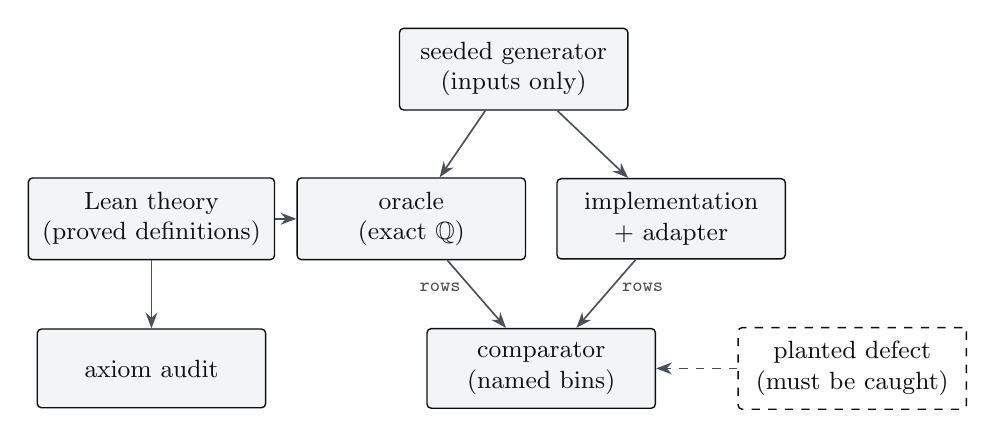
\begin{tikzpicture}[
  box/.style={draw=Ink, line width=0.5pt, fill=Surface, text=Ink, rounded corners=1.5pt,
    align=center, font=\small, inner sep=5pt, minimum height=10mm, minimum width=29mm},
  arr/.style={-{Stealth[length=2mm]}, line width=0.6pt, draw=InkMuted},
  lab/.style={font=\ttfamily\scriptsize, text=InkMuted}]
\node[box] (gen) at (4.6,1.9) {seeded generator\\(inputs only)};
\node[box] (theory) at (0,0) {Lean theory\\(proved definitions)};
\node[box] (oracle) at (3.3,0) {oracle\\(exact $\mathbb{Q}$)};
\node[box] (impl) at (6.6,0) {implementation\\+ adapter};
\node[box] (cmp) at (4.95,-1.9) {comparator\\(named bins)};
\node[box] (audit) at (0,-1.9) {axiom audit};
\node[box, dashed, fill=Background] (planted) at (8.9,-1.9) {planted defect\\(must be caught)};
\draw[arr] (gen) -- (oracle);
\draw[arr] (gen) -- (impl);
\draw[arr] (theory) -- (oracle);
\draw[arr] (theory) -- (audit);
\draw[arr] (oracle) -- node[left, lab, pos=0.4] {rows} (cmp);
\draw[arr] (impl) -- node[right, lab, pos=0.4] {rows} (cmp);
\draw[arr, dashed] (planted) -- (cmp);
\end{tikzpicture}
\caption{The measurement procedure. The generator never computes expected results;
those come only from the oracle.}
\label{fig:harness}
\end{figure}

The procedure follows \texttt{ledger-semantics} (\cref{fig:harness}). A seeded
generator writes case files containing inputs only. It favors the inputs where
implementations are known to have conventions: tied logits, words that are
themselves tokens, and merge tables with several splits of one string. A small
adapter per implementation runs the same cases and prints the oracle's row format.
The comparator places every case in exactly one named bin (agree, diverge, skipped
by either side, or missing), so nothing is dropped silently. Token rows are compared
as strings. Sampler rows require that a zero be matched by a zero and that nonzero
probabilities agree within $10^{-6}$, since llama.cpp stores logits in
\texttt{float32}. Each comparator is observed to fail: a planted defect, an adapter
that glues two tokens or one that inverts temperature, must be detected or the run
fails.

\paragraph{Tie divergences.} An implementation that keeps exactly $k$ tokens breaks
ties in its own order, which need not be the oracle's order by index. Every filter
treats tied tokens alike except for that choice, and tied tokens stay tied through
temperature and renormalization. Such an implementation must therefore agree with
the positional semantics up to a permutation of tied tokens. The harness checks
exactly this: the multiset of (logit, probability) pairs over the kept tokens must
equal that of the oracle's \texttt{q} rows. A divergence that fails this check is
reported as unexplained.

\begin{table}[t]
\centering\small
\caption{Measurements (\texttt{harness/run.sh 600}: four seeds of 600 cases each per
corpus). Lean 4.34.1, Mathlib v4.34.1, \texttt{tokenizers} 0.23.3, \texttt{tiktoken}
0.14.0, llama.cpp commit \texttt{a9d27ac} (2026-10-11).}
\label{tab:results}
\begin{tabularx}{\linewidth}{@{}>{\raggedright\arraybackslash}p{4.6cm}>{\raggedright\arraybackslash}X>{\raggedright\arraybackslash}X@{}}
\toprule
\qpth{Implementation} & \qpth{Compared against} & \qpth{Result}\\
\midrule
HF \texttt{tokenizers}, BPE, defaults & rule-rank BPE (\lean{bpe}) & 13{,}779 / 13{,}779 words identical\\
HF \texttt{tokenizers}, \lean{ignore_merges} & lookup, then rule-rank BPE & 13{,}779 / 13{,}779 identical\\
\texttt{tiktoken} & lookup, then concatenation-rank BPE & 13{,}779 / 13{,}779 identical\\
llama.cpp \lean{top_k}, \lean{top_p}, \lean{min_p}, \texttt{temp}, no ties & tie-keeping filters & 1{,}216 / 1{,}216 chains, $|\Delta p|\le5.1\times10^{-8}$\\
llama.cpp, with ties & tie-keeping, else positional & 939 + 245 / 1{,}184 chains; 0 unexplained\\
Planted defects (tokenizer, sampler) & --- & both detected\\
\bottomrule
\end{tabularx}
\end{table}

\Cref{tab:results} summarizes the results. Two findings came out of the
comparisons. First, \texttt{tiktoken} initially disagreed with the oracle's
concatenation-rank BPE on words that are themselves vocabulary tokens. The
disagreement was a convention, whole-word lookup. Following the
\texttt{ledger-semantics} rule that a divergence is either a defect in the
implementation or a convention the semantics has not yet recorded, we recorded it
as \lean{lookupFirst}, with its own theorems, after which agreement is exact.
Second, on the same random merge tables the two tokenizer libraries disagree with
each other on 439 of 13{,}779 words (3.2\%), and on 279 when Hugging Face uses
\lean{ignore_merges}. The oracle reproduces each library exactly, so every one of
these disagreements is predicted. \Cref{thm:bpeconv} states the condition under which
they cannot occur.

For sampling, llama.cpp agrees with the tie-keeping semantics on every tie-free
chain. On chains with ties, 245 of 1{,}184 diverge, and every one agrees with the
positional semantics up to a permutation of tied tokens. Some of these divergences
cascade: a tie cut by top-$k$ changes the renormalized masses that a later top-$p$
sees. A check that compared kept sets only after the fact would misclassify such
cases. Replaying the convention exactly classifies all of them.

% ===========================================================================
\section{Related work}

\paragraph{Formal methods for machine learning.} Most verification work on neural
networks proves properties of trained models, for example with SMT-based
methods~\cite{katz2017reluplex}. We verify the model-independent algorithms around
the model instead, and connect them to implementations through an oracle. The
denotational method follows Elliott~\cite{elliott2009denotational}. The use of a
proved semantics as a test oracle, the procedure of planted defects, and the
discipline of named skip bins follow \texttt{ledger-semantics}~\cite{ledgersemantics}.
Our category of finite stochastic maps is a special case of Fritz's Markov
categories~\cite{fritz2020markov}.

\paragraph{Tokenization.} Zouhar et al.\ give a formal analysis of BPE as an
optimization problem~\cite{zouhar2023bpe}. Gastaldi et al.\ treat tokenizers as
stochastic maps and study consistency of estimators~\cite{gastaldi2024foundations}.
Vieira et al.\ show how to turn token-level models into character-level
ones~\cite{vieira2024tokens}, which requires exactly the enumeration of
tokenizations we verify. Our no-compression theorem and the agreement criterion
between BPE conventions complement this work at the level of exact identities.

\paragraph{Decoding.} Top-$k$~\cite{fan2018hierarchical}, nucleus~\cite{holtzman2020curious}
and min-$p$~\cite{nguyen2025minp} sampling are usually specified by an algorithm over
sorted arrays, which leaves ties unspecified. \Cref{thm:topk} shows that this gap
cannot be closed by any symmetric rule. Speculative
sampling~\cite{leviathan2023speculative,chen2023speculative} is known to be lossless,
and its acceptance rate is the maximal-coupling bound~\cite{lindvall1992coupling}. Du et
al.\ characterize tightness measure-theoretically~\cite{du2023tight}. We give a
finite-depth statement and an explicit non-tight model.

\paragraph{Attention and inference systems.} Online softmax~\cite{milakov2018online}
underlies FlashAttention~\cite{dao2022flashattention} and its successors, and
KV caching is standard in serving systems~\cite{pope2023scaling,kwon2023vllm}. Our
contribution is the algebraic packaging, a commutative monoid with a free-monoid
homomorphism, and machine-checked proofs over arbitrary exponential characters.
Permutation equivariance of attention without positional encodings is
known~\cite{yun2020universal}.

\paragraph{Masked diffusion.} The time-independence of the optimal denoiser was
observed by Ou et al.~\cite{ou2025absorbing}, in the setting of
D3PM~\cite{austin2021d3pm}, MDLM~\cite{sahoo2024mdlm} and related
models~\cite{shi2024masked,nie2025llada}. We machine-check it, together with the
any-order chain rule and the inexactness of parallel unmasking.

% ===========================================================================
\section{Limitations}

Analysis on the reals enters only through exponential characters, and there is no
measure theory, so sampling and tightness are stated through finite quantities. The
oracle's temperature is restricted to $1/n$, which keeps softmax rational. The
theorems hold for every temperature, but the oracle cannot evaluate an irrational
softmax. Speculative decoding is proved for one drafted token. The sequence version
follows by induction and is not yet formalized. Nothing is proved about
floating-point arithmetic: implementations are compared with exact values within a
stated tolerance. A decision that lies exactly on a floating-point boundary could in
principle diverge, and none occurred in our runs. The diffusion theory covers
absorbing diffusion, not Gaussian diffusion. The chat protocol models tool calling in
its common request-and-result form, not any vendor's specification. The measurements
cover tokenizers and samplers; attention kernels, speculative decoders, chat
renderers and diffusion samplers are evaluated by the oracle but not yet compared
against implementations.

% ===========================================================================
\section{Conclusion}

The inference side of LLMs is small enough to be given a precise meaning and large
enough that its implementations disagree. A machine-checked semantics separates
what is meaning from what is convention. It proves which reorderings, cachings and
tilings are harmless, and it shows that some properties folklore expects, such as
symmetric exact top-$k$, compositional compressing tokenizers and unambiguous plain-text
templates, cannot exist. Connected to an exact oracle, the same definitions become
a test instrument. Every divergence it surfaces is either a defect in an
implementation or a convention that belongs in the semantics.

\paragraph{Availability.} The Lean development, oracle, harness, and recorded
measurement log accompany this paper.

\paragraph{Acknowledgments.} The structure of this work follows
\texttt{ledger-semantics} by John Wiegley. The formalization and harness were
developed with the assistance of an AI system (Claude, Anthropic).

% ===========================================================================
\begin{thebibliography}{99}\small

\bibitem{austin2021d3pm}
J.~Austin, D.~D. Johnson, J.~Ho, D.~Tarlow, and R.~van~den Berg.
\newblock Structured denoising diffusion models in discrete state-spaces.
\newblock In \emph{NeurIPS}, 2021.

\bibitem{chen2023speculative}
C.~Chen, S.~Borgeaud, G.~Irving, J.-B. Lespiau, L.~Sifre, and J.~Jumper.
\newblock Accelerating large language model decoding with speculative sampling.
\newblock arXiv:2302.01318, 2023.

\bibitem{dao2022flashattention}
T.~Dao, D.~Y. Fu, S.~Ermon, A.~Rudra, and C.~R{\'e}.
\newblock {FlashAttention}: Fast and memory-efficient exact attention with {IO}-awareness.
\newblock In \emph{NeurIPS}, 2022.

\bibitem{demoura2021lean4}
L.~de~Moura and S.~Ullrich.
\newblock The {Lean} 4 theorem prover and programming language.
\newblock In \emph{CADE-28}, 2021.

\bibitem{du2023tight}
L.~Du, L.~Torroba~Hennigen, T.~Pimentel, C.~Meister, J.~Eisner, and R.~Cotterell.
\newblock A measure-theoretic characterization of tight language models.
\newblock In \emph{ACL}, 2023.

\bibitem{elliott2009denotational}
C.~Elliott.
\newblock Denotational design with type class morphisms.
\newblock Technical Report 2009-01, LambdaPix, 2009.

\bibitem{fan2018hierarchical}
A.~Fan, M.~Lewis, and Y.~Dauphin.
\newblock Hierarchical neural story generation.
\newblock In \emph{ACL}, 2018.

\bibitem{fritz2020markov}
T.~Fritz.
\newblock A synthetic approach to {Markov} kernels, conditional independence and theorems on sufficient statistics.
\newblock \emph{Advances in Mathematics}, 370, 2020.

\bibitem{gastaldi2024foundations}
J.~L. Gastaldi, J.~Terilla, L.~Malagutti, B.~DuSell, T.~Vieira, and R.~Cotterell.
\newblock The foundations of tokenization: Statistical and computational concerns.
\newblock arXiv:2407.11606, 2024.

\bibitem{greshake2023injection}
K.~Greshake, S.~Abdelnabi, S.~Mishra, C.~Endres, T.~Holz, and M.~Fritz.
\newblock Not what you've signed up for: Compromising real-world {LLM}-integrated applications with indirect prompt injection.
\newblock In \emph{AISec}, 2023.

\bibitem{holtzman2020curious}
A.~Holtzman, J.~Buys, L.~Du, M.~Forbes, and Y.~Choi.
\newblock The curious case of neural text degeneration.
\newblock In \emph{ICLR}, 2020.

\bibitem{katz2017reluplex}
G.~Katz, C.~Barrett, D.~L. Dill, K.~Julian, and M.~J. Kochenderfer.
\newblock Reluplex: An efficient {SMT} solver for verifying deep neural networks.
\newblock In \emph{CAV}, 2017.

\bibitem{kwon2023vllm}
W.~Kwon, Z.~Li, S.~Zhuang, Y.~Sheng, L.~Zheng, C.~H. Yu, J.~E. Gonzalez, H.~Zhang, and I.~Stoica.
\newblock Efficient memory management for large language model serving with {PagedAttention}.
\newblock In \emph{SOSP}, 2023.

\bibitem{ledgersemantics}
J.~Wiegley.
\newblock ledger-semantics: Mathematical semantics of {Ledger}, the double-entry accounting tool.
\newblock \url{https://github.com/ledger/ledger-semantics}, 2026.

\bibitem{leviathan2023speculative}
Y.~Leviathan, M.~Kalman, and Y.~Matias.
\newblock Fast inference from transformers via speculative decoding.
\newblock In \emph{ICML}, 2023.

\bibitem{lindvall1992coupling}
T.~Lindvall.
\newblock \emph{Lectures on the Coupling Method}.
\newblock Wiley, 1992.

\bibitem{liu2023ring}
H.~Liu, M.~Zaharia, and P.~Abbeel.
\newblock Ring attention with blockwise transformers for near-infinite context.
\newblock arXiv:2310.01889, 2023.

\bibitem{mathlib2020}
The mathlib Community.
\newblock The {Lean} mathematical library.
\newblock In \emph{CPP}, 2020.

\bibitem{milakov2018online}
M.~Milakov and N.~Gimelshein.
\newblock Online normalizer calculation for softmax.
\newblock arXiv:1805.02867, 2018.

\bibitem{nguyen2025minp}
M.~N. Nguyen, A.~Baker, C.~Neo, A.~Roush, A.~Kirsch, and R.~Shwartz-Ziv.
\newblock Turning up the heat: Min-p sampling for creative and coherent {LLM} outputs.
\newblock In \emph{ICLR}, 2025.

\bibitem{nie2025llada}
S.~Nie, F.~Zhu, Z.~You, X.~Zhang, J.~Ou, J.~Hu, J.~Zhou, Y.~Lin, J.-R. Wen, and C.~Li.
\newblock Large language diffusion models.
\newblock arXiv:2502.09992, 2025.

\bibitem{ou2025absorbing}
J.~Ou, S.~Nie, K.~Xue, F.~Zhu, J.~Sun, Z.~Li, and C.~Li.
\newblock Your absorbing discrete diffusion secretly models the conditional distributions of clean data.
\newblock In \emph{ICLR}, 2025.

\bibitem{pope2023scaling}
R.~Pope, S.~Douglas, A.~Chowdhery, J.~Devlin, J.~Bradbury, J.~Heek, K.~Xiao, S.~Agrawal, and J.~Dean.
\newblock Efficiently scaling transformer inference.
\newblock In \emph{MLSys}, 2023.

\bibitem{rabe2021selfattention}
M.~N. Rabe and C.~Staats.
\newblock Self-attention does not need {$O(n^2)$} memory.
\newblock arXiv:2112.05682, 2021.

\bibitem{radford2019gpt2}
A.~Radford, J.~Wu, R.~Child, D.~Luan, D.~Amodei, and I.~Sutskever.
\newblock Language models are unsupervised multitask learners.
\newblock OpenAI technical report, 2019.

\bibitem{sahoo2024mdlm}
S.~S. Sahoo, M.~Arriola, Y.~Schiff, A.~Gokaslan, E.~Marroquin, J.~T. Chiu, A.~Rush, and V.~Kuleshov.
\newblock Simple and effective masked diffusion language models.
\newblock In \emph{NeurIPS}, 2024.

\bibitem{sennrich2016bpe}
R.~Sennrich, B.~Haddow, and A.~Birch.
\newblock Neural machine translation of rare words with subword units.
\newblock In \emph{ACL}, 2016.

\bibitem{shi2024masked}
J.~Shi, K.~Han, Z.~Wang, A.~Doucet, and M.~K. Titsias.
\newblock Simplified and generalized masked diffusion for discrete data.
\newblock In \emph{NeurIPS}, 2024.

\bibitem{vieira2024tokens}
T.~Vieira, B.~LeBrun, M.~Giulianelli, J.~L. Gastaldi, B.~DuSell, J.~Terilla, T.~J. O'Donnell, and R.~Cotterell.
\newblock From language models over tokens to language models over characters.
\newblock arXiv:2412.03719, 2024.

\bibitem{wolf2020transformers}
T.~Wolf et~al.
\newblock Transformers: State-of-the-art natural language processing.
\newblock In \emph{EMNLP: System Demonstrations}, 2020.

\bibitem{xiao2024sinks}
G.~Xiao, Y.~Tian, B.~Chen, S.~Han, and M.~Lewis.
\newblock Efficient streaming language models with attention sinks.
\newblock In \emph{ICLR}, 2024.

\bibitem{yun2020universal}
C.~Yun, S.~Bhojanapalli, A.~S. Rawat, S.~J. Reddi, and S.~Kumar.
\newblock Are transformers universal approximators of sequence-to-sequence functions?
\newblock In \emph{ICLR}, 2020.

\bibitem{zouhar2023bpe}
V.~Zouhar, C.~Meister, J.~L. Gastaldi, L.~Du, T.~Vieira, M.~Sachan, and R.~Cotterell.
\newblock A formal perspective on byte-pair encoding.
\newblock In \emph{Findings of ACL}, 2023.

\end{thebibliography}

\end{document}
"
% ---------------------------------------------------------------------------
\documentclass[10pt]{article}

\newif\ifqptdark
\qptdarkfalse   % print edition (light). \qptdarktrue gives the dark screen edition.
\ifdefined\qptdarkedition\qptdarktrue\fi  % or: xelatex "\def\qptdarkedition{}% !TeX program = xelatex
% ---------------------------------------------------------------------------
%  A Machine-Checked Semantics of LLM Inference
%  Daniel Arango Sohm, Universidad EAFIT
%
%  Typeset in the QPT visual design system:
%    * neutral-first: Ink on Background carries the document;
%    * paradigm colours are semantic only. This paper belongs to none of the
%      five paradigms, so no paradigm colour appears in its content; the
%      colours appear only in the QPT mark itself;
%    * no gradients;
%    * Space Grotesk for display, Inter for body text, IBM Plex Mono for
%      technical, numeric, label, code and proof-oriented content.
%
%  Compile with:  xelatex llm-semantics-qpt.tex   (twice, for references)
%  Dark screen edition: set \qptdarktrue below, or run
%    xelatex -jobname=llm-semantics-qpt-dark "\def\qptdarkedition{}% !TeX program = xelatex
% ---------------------------------------------------------------------------
%  A Machine-Checked Semantics of LLM Inference
%  Daniel Arango Sohm, Universidad EAFIT
%
%  Typeset in the QPT visual design system:
%    * neutral-first: Ink on Background carries the document;
%    * paradigm colours are semantic only. This paper belongs to none of the
%      five paradigms, so no paradigm colour appears in its content; the
%      colours appear only in the QPT mark itself;
%    * no gradients;
%    * Space Grotesk for display, Inter for body text, IBM Plex Mono for
%      technical, numeric, label, code and proof-oriented content.
%
%  Compile with:  xelatex llm-semantics-qpt.tex   (twice, for references)
%  Dark screen edition: set \qptdarktrue below, or run
%    xelatex -jobname=llm-semantics-qpt-dark "\def\qptdarkedition{}\input{llm-semantics-qpt}"
% ---------------------------------------------------------------------------
\documentclass[10pt]{article}

\newif\ifqptdark
\qptdarkfalse   % print edition (light). \qptdarktrue gives the dark screen edition.
\ifdefined\qptdarkedition\qptdarktrue\fi  % or: xelatex "\def\qptdarkedition{}\input{llm-semantics-qpt}"

\usepackage[a4paper,textwidth=15.4cm,textheight=23.6cm,top=3.0cm,headsep=0.9cm,footskip=1.2cm]{geometry}
\usepackage{amsmath,amssymb,amsthm,mathtools}
\usepackage{fontspec}
\usepackage{booktabs,tabularx,array}
\usepackage[protrusion=true,expansion=false]{microtype}
\usepackage[table]{xcolor}
\usepackage{graphicx}
\usepackage{fvextra}
\usepackage{enumitem}
\usepackage{caption}
\usepackage{titlesec}
\usepackage{fancyhdr}
\usepackage[most]{tcolorbox}
\usepackage{tikz}
\usetikzlibrary{arrows.meta}
\usepackage{hyperref}
\usepackage[nameinlink,capitalise]{cleveref}

% ---------------------------------------------------------------------------
%  Colour tokens
% ---------------------------------------------------------------------------
% Neutral foundation. Ink and Background invert between the two editions.
\ifqptdark
  \definecolor{Background}{HTML}{0B0C0E}
  \definecolor{Surface}{HTML}{16181B}
  \definecolor{Border}{HTML}{2B2E33}
  \definecolor{Ink}{HTML}{EDEEF0}
  \definecolor{InkMuted}{HTML}{A9AEB6}
  \definecolor{InkFaint}{HTML}{5A5F67}   % decoration only, never meaningful text
\else
  \definecolor{Background}{HTML}{FFFFFF}
  \definecolor{Surface}{HTML}{F3F4F5}
  \definecolor{Border}{HTML}{DADDE1}
  \definecolor{Ink}{HTML}{0E0F11}
  \definecolor{InkMuted}{HTML}{4B4F57}
  \definecolor{InkFaint}{HTML}{A3A7AE}   % decoration only, never meaningful text
\fi
% Paradigm colours: fixed in both editions, semantic only.
\definecolor{Quantum}{HTML}{5BAD1E}
\definecolor{Photonic}{HTML}{F0AB00}
\definecolor{Thermodynamic}{HTML}{E8690A}
\definecolor{Ternary}{HTML}{8A8A8A}
\definecolor{Bio}{HTML}{1AAB7C}

\ifqptdark\pagecolor{Background}\fi

% ---------------------------------------------------------------------------
%  Typography
% ---------------------------------------------------------------------------
\setmainfont{Inter}[
  Path=fonts/, Extension=.otf, Scale=0.94,
  UprightFont=*-Regular, ItalicFont=*-Italic,
  BoldFont=*-SemiBold, BoldItalicFont=*-SemiBoldItalic]
\setmonofont{IBMPlexMono}[
  Path=fonts/, Extension=.ttf, Scale=MatchLowercase,
  UprightFont=*-Regular, ItalicFont=*-Italic, BoldFont=*-SemiBold]
\newfontfamily\qptdisplay{SpaceGrotesk}[
  Path=fonts/, Extension=.otf, UprightFont=*-Medium, BoldFont=*-Bold]
\newfontfamily\qptdisplaylight{SpaceGrotesk}[
  Path=fonts/, Extension=.otf, UprightFont=*-Regular]
\newfontfamily\qptlabelfont{IBMPlexMono}[
  Path=fonts/, Extension=.ttf, Scale=MatchLowercase, UprightFont=*-Medium,
  LetterSpace=6]
\setsansfont{Inter}[
  Path=fonts/, Extension=.otf, Scale=0.94,
  UprightFont=*-Regular, ItalicFont=*-Italic,
  BoldFont=*-SemiBold, BoldItalicFont=*-SemiBoldItalic]
\linespread{1.16}
\setlength{\emergencystretch}{2.5em}
\AtBeginDocument{\raggedright\setlength{\parindent}{0pt}}
\setlength{\parindent}{0pt}
\setlength{\parskip}{0.55em}

% A label: IBM Plex Mono, upper case, tracked.
\newcommand{\qptlabel}[1]{{\qptlabelfont\footnotesize\MakeUppercase{#1}}}
% Technical names (Lean declarations, files) in IBM Plex Mono.
\newcommand{\lean}[1]{\texttt{\detokenize{#1}}}
\newcommand{\leanref}[1]{\par\smallskip\noindent
  {\ttfamily\footnotesize\upshape\raggedright\color{InkMuted}LEAN\enspace #1\par}}

% Ink is the normal colour everywhere, including floats, heads and footnotes.
\makeatletter
\AtBeginDocument{\color{Ink}\global\let\default@color\current@color}
\makeatother

% ---------------------------------------------------------------------------
%  Mathematical notation
% ---------------------------------------------------------------------------
\newcommand{\K}{\Bbbk}
\newcommand{\Dist}{\mathrm{Dist}}
\newcommand{\restr}[2]{#1|_{#2}}
\newcommand{\topk}{\mathrm{TopK}}
\newcommand{\topp}{\mathrm{TopP}}
\newcommand{\minp}{\mathrm{MinP}}
\newcommand{\sharpen}{\mathrm{sharpen}}
\newcommand{\abv}{\mathrm{above}}
\newcommand{\tv}{\mathrm{tv}}
\newcommand{\dec}{\mathrm{dec}}
\newcommand{\enc}{\mathrm{enc}}
\newcommand{\softmax}{\mathrm{softmax}}
\newcommand{\attend}{\mathrm{attend}}
\newcommand{\Iv}[1]{[\![#1]\!]}
\newcommand{\Mask}{\bot}

% ---------------------------------------------------------------------------
%  Headings: section numbers as labels, titles in Space Grotesk
% ---------------------------------------------------------------------------
\makeatletter
\newcommand{\qptsecnum}[1]{{\qptlabelfont\small\color{InkMuted}\two@digits{#1}}}
\makeatother
\titleformat{\section}
  {\qptdisplay\fontsize{14.5}{18}\selectfont\color{Ink}}
  {\qptsecnum{\value{section}}}{0.9em}{}
\titleformat{name=\section,numberless}
  {\qptdisplay\fontsize{14.5}{18}\selectfont\color{Ink}}{}{0pt}{}
\titlespacing*{\section}{0pt}{1.9em}{0.7em}
\titleformat{\paragraph}[runin]
  {\qptdisplay\normalsize\color{Ink}}{}{0pt}{}
\titlespacing*{\paragraph}{0pt}{0.9em}{0.6em}

% ---------------------------------------------------------------------------
%  Statements
% ---------------------------------------------------------------------------
\newtheoremstyle{qpt}
  {0.9em}{0.9em}
  {\normalfont}{}
  {\qptlabelfont\footnotesize}{}
  {\newline}
  {\MakeUppercase{\thmname{#1}\thmnumber{~#2}}%
   \thmnote{\enspace{\qptdisplay\normalsize\color{Ink}#3}}}
\theoremstyle{qpt}
\newtheorem{theorem}{Theorem}
\newtheorem{proposition}[theorem]{Proposition}
\newtheorem{corollary}[theorem]{Corollary}
\newtheorem{lemma}[theorem]{Lemma}
\newtheorem{definition}[theorem]{Definition}
\newtheorem{remark}[theorem]{Remark}

% Proofs: a tracked label and a neutral end mark.
\makeatletter
\renewcommand{\qedsymbol}{{\color{InkMuted}\rule{0.5em}{0.5em}}}
\renewenvironment{proof}[1][Proof]{\par\pushQED{\qed}\normalfont\topsep0.5em\relax
  \trivlist\item[\hskip\labelsep\qptlabel{#1}\hspace{0.6em}]\ignorespaces}
  {\popQED\endtrivlist\@endpefalse}
\makeatother

% ---------------------------------------------------------------------------
%  Code: IBM Plex Mono on a neutral surface, with a hairline on the left
% ---------------------------------------------------------------------------
\tcbset{colupper=Ink, collower=Ink}
\tcbset{qptcode/.style={enhanced, colback=Surface, colframe=Surface,
  boxrule=0pt, arc=0pt, left=9pt, right=8pt, top=5pt, bottom=5pt,
  borderline west={1.2pt}{0pt}{InkFaint}, before skip=0.7em, after skip=0.7em}}
\newenvironment{leancode}
  {\VerbatimEnvironment\begin{tcolorbox}[qptcode]%
   \begin{Verbatim}[fontsize=\small,commandchars=\\\{\},
     codes={\catcode`\$=3\catcode`\^=7},formatcom=\color{Ink}]}
  {\end{Verbatim}\end{tcolorbox}}
\newenvironment{casecode}
  {\VerbatimEnvironment\begin{tcolorbox}[qptcode,before skip=0pt,after skip=0pt]%
   \begin{Verbatim}[fontsize=\footnotesize,formatcom=\color{Ink}]}
  {\end{Verbatim}\end{tcolorbox}}

% ---------------------------------------------------------------------------
%  Floats, tables, captions
% ---------------------------------------------------------------------------
\DeclareCaptionLabelFormat{qpt}{\qptlabel{#1~#2}}
\DeclareCaptionLabelSeparator{qptsep}{\quad}
\captionsetup{labelformat=qpt, labelsep=qptsep, font={small,color=Ink},
  justification=raggedright, singlelinecheck=false, skip=6pt}
\newcommand{\qpth}[1]{\qptlabel{#1}}
\arrayrulecolor{Ink}
\setlength{\heavyrulewidth}{0.7pt}
\setlength{\lightrulewidth}{0.35pt}
\renewcommand{\arraystretch}{1.22}

% ---------------------------------------------------------------------------
%  Running heads
% ---------------------------------------------------------------------------
\pagestyle{fancy}
\fancyhf{}
\fancyhead[L]{{\color{Ink}\qptlabel{Machine-checked semantics of LLM inference}}}
\fancyhead[R]{{\color{Ink}\qptlabel{D. Arango Sohm}}}
\fancyfoot[R]{{\ttfamily\small\color{InkMuted}\thepage}}
\renewcommand{\headrule}{{\color{Border}\hrule height 0.4pt}\vspace{-0.4pt}}
\renewcommand{\headrulewidth}{0.4pt}
\fancypagestyle{qptfirst}{\fancyhf{}%
  \fancyfoot[R]{{\ttfamily\small\color{InkMuted}\thepage}}%
  \renewcommand{\headrulewidth}{0pt}\renewcommand{\headrule}{}}

% ---------------------------------------------------------------------------
%  Links and references: neutral, never accent-coloured text
% ---------------------------------------------------------------------------
\hypersetup{colorlinks=true, linkcolor=Ink, citecolor=Ink, urlcolor=Ink,
  pdftitle={A Machine-Checked Semantics of LLM Inference},
  pdfauthor={Daniel Arango Sohm},
  pdfsubject={Formal semantics of large language model inference in Lean 4},
  pdfkeywords={Lean 4, Mathlib, formal verification, LLM inference, sampling,
    tokenization, attention, speculative decoding, diffusion language models}}
\makeatletter
\renewcommand{\@biblabel}[1]{{\ttfamily\color{InkMuted}[#1]}}
\renewcommand{\@cite}[2]{{\ttfamily[#1\if@tempswa, #2\fi]}}
\makeatother
\renewcommand{\refname}{References}

\setlist{itemsep=2pt, topsep=4pt}
\setlist[itemize]{label={\color{InkMuted}\textbullet}}

\begin{document}
\thispagestyle{qptfirst}

% ----------------------------------------------------------------- masthead
\noindent
\begin{minipage}[c]{0.5\linewidth}
  \includegraphics[height=1.9cm]{qpt-logo.png}
\end{minipage}%
\begin{minipage}[c]{0.5\linewidth}\raggedleft
  \qptlabel{Preprint}\\[2pt]
  \qptlabel{October 2026}
\end{minipage}

\vspace{1.6em}
{\color{Border}\rule{\linewidth}{0.4pt}}
\vspace{1.1em}

{\qptdisplay\fontsize{25}{29.5}\selectfont\color{Ink}
A Machine-Checked Semantics\\ of LLM Inference\par}
\vspace{0.55em}
{\qptdisplaylight\fontsize{13}{17}\selectfont\color{InkMuted}
Sampling, Attention, Tokenization, Chat, Decoding,\\ and Diffusion in Lean~4\par}

\vspace{1.5em}
{\large\bfseries Daniel Arango Sohm}\par
\vspace{0.15em}
{\color{InkMuted}Universidad EAFIT, Medellín, Colombia\\
Former member of the QPT team}\par

\vspace{1.4em}
% ----------------------------------------------------------------- abstract
\begin{tcolorbox}[enhanced, colback=Surface, colframe=Surface, colupper=Ink, boxrule=0pt,
  arc=0pt, left=12pt, right=12pt, top=9pt, bottom=10pt]
\qptlabel{Abstract}\par\vspace{0.35em}
{\small
The inference side of a large language model is a stack of small algorithms:
tokenizers, attention kernels, key--value caches, sampling filters, speculative
decoders, chat templates, and diffusion samplers. Each has several independent
implementations, and those implementations are usually tested against one another
rather than against a definition. We give these components a single mathematical
semantics, formalized in Lean~4 against Mathlib. The development comprises about
4{,}600 lines and 270 named theorems, and every declaration depends only on Lean's
three standard axioms. It proves the exact algebra of sampling filters, the
losslessness and optimality of speculative sampling, and the correctness of
key--value caching and of FlashAttention-style online softmax as a commutative
monoid. It proves that byte-pair encoding is lossless under every merge priority,
together with a decidable criterion for when the Hugging Face and \texttt{tiktoken}
conventions agree, a protocol checker for tool calls, and the time-independence of
the masked-diffusion denoiser. It also proves six negative results. No sampling
rule that treats tokens symmetrically can always keep exactly $k$ tokens. No
tokenizer that compresses can respect concatenation. Every chat template that writes
its role markers in the content alphabet is ambiguous. No transformer without
positional information can copy a fixed position. An autoregressive model need not
define a distribution over strings. Parallel unmasking in diffusion is inexact.
From the same definitions we build an executable oracle that evaluates test cases in
exact rational arithmetic, and a harness that measures implementations against it.
On 2{,}400 random merge tables, Hugging Face \texttt{tokenizers} and
\texttt{tiktoken} each agree with the oracle on all 13{,}779 test words, while
disagreeing with each other on 3.2\% of them. On 2{,}400 random sampler chains,
every divergence of llama.cpp from the tie-keeping semantics is accounted for
exactly by the positional semantics that the impossibility theorem forces.
\par}
\end{tcolorbox}

\vspace{0.3em}
\noindent\qptlabel{Keywords}\enspace{\small Lean~4 · Mathlib · formal verification ·
LLM inference · sampling · tokenization · attention · speculative decoding ·
diffusion language models}

\vspace{0.4em}
{\color{Border}\rule{\linewidth}{0.4pt}}

% ===========================================================================
\section{Introduction}

A deployed language model is a function from parameters and a context to a
distribution over tokens. Turning that distribution into text requires more
machinery. A tokenizer maps strings to token sequences. Attention kernels compute
the model's reads over a cached context. A chain of sampling filters reshapes the
next-token distribution. A speculative decoder may verify drafted tokens, a chat
template linearizes a conversation, and a diffusion sampler may unmask several
positions at once. Each of these components exists in many implementations, such as
Hugging Face \texttt{transformers} and \texttt{tokenizers}~\cite{wolf2020transformers},
\texttt{tiktoken}, vLLM~\cite{kwon2023vllm}, and llama.cpp. Their tests mostly
compare one implementation with another, or with remembered behavior.

This paper follows a different discipline, \emph{denotational design}~\cite{elliott2009denotational}.
One first says precisely what a thing means, then requires every operation to
preserve that meaning, and lets the implementation be whatever the equations force
it to be. The approach is that of \texttt{ledger-semantics}~\cite{ledgersemantics},
which formalizes double-entry accounting in Lean and uses the result as a test oracle
for the C++ Ledger program. We apply it to LLM inference. A sampling filter means
conditioning a distribution on a set. A KV-cached decoder means causal attention over
the whole prefix. A FlashAttention kernel means a softmax-weighted average. A chat
template means an injective encoding of a transcript. The theorems state when an
implementation preserves that meaning, and several of them state that no
implementation can.

\paragraph{Contributions.}
\begin{itemize}[leftmargin=*,itemsep=2pt]
\item A Lean~4 formalization against Mathlib~\cite{mathlib2020,demoura2021lean4}
  of sampling, speculative decoding, softmax and attention, tokenization, chat
  transcripts, autoregressive decoding, and masked diffusion
  (\cref{sec:foundations,sec:sampling,sec:spec,sec:attention,sec:tokenization,sec:chat,sec:decoding,sec:diffusion}).
  All definitions are stated over an arbitrary linearly ordered field, so one proof
  covers the real numbers of the literature and the exact rationals of the oracle.
\item Positive results in a common framework. They include the algebra of
  sampling filters, the optimality of speculative sampling, an online-softmax
  commutative monoid, a generic correctness theorem for BPE with a decidable
  agreement criterion between the two conventions in use, a protocol checker for
  tool calls, and the any-order chain rule for masked diffusion.
\item Six negative results that explain design constraints visible across
  implementations (\cref{sec:negative}).
\item An executable oracle that evaluates case files under the proved
  definitions in exact arithmetic, and a measurement of Hugging Face
  \texttt{tokenizers}, \texttt{tiktoken}, and llama.cpp against it (\cref{sec:oracle,sec:measure}).
\end{itemize}

Several of the positive results are known: losslessness of speculative
sampling~\cite{leviathan2023speculative,chen2023speculative}, correctness of online
softmax~\cite{milakov2018online,dao2022flashattention}, time-independence of the
absorbing-diffusion posterior~\cite{ou2025absorbing}, and the role of permutation
equivariance~\cite{yun2020universal}. Our contribution for these is a machine-checked
statement in one framework, connected to an oracle. To our knowledge the
following are not stated elsewhere in the form given here: the impossibility of
symmetric exact top-$k$ and nucleus selection, the no-compression theorem for
homomorphic tokenizers, the ambiguity of every in-band chat template, and the
decidable agreement criterion between merge-rule and concatenation-rank BPE.

% ===========================================================================
\section{Method and trust base}\label{sec:method}

The development is a Lean~4 library (Lean 4.34.1, Mathlib v4.34.1) of eleven
theory modules and two executable modules (\cref{tab:modules}). It is built with
warnings promoted to errors, so an unproved theorem (\lean{sorry}) fails the build.
A separate audit program walks every declaration in the library, 853 in all, and
fails unless each depends only on propositional extensionality, the axiom of choice,
and quotient soundness. The audit has been observed to fail: a planted proof by
\lean{native_decide}, which introduces an auxiliary axiom trusting compiled code, is
rejected. The warnings-as-errors build alone does not catch it. Concrete
counterexamples are therefore proved by \lean{decide}, whose certificate the kernel
checks by evaluation.

\begin{table}[t]
\centering\small
\caption{Modules of the development. Lines and named theorems and lemmas per module.}
\label{tab:modules}
\begin{tabularx}{\linewidth}{@{}l>{\raggedright\arraybackslash}X>{\ttfamily}r>{\ttfamily}r@{}}
\toprule
\qpth{Module} & \qpth{Content} & \qpth{Lines} & \qpth{Thms} \\
\midrule
\lean{Dist} & finite distributions, conditioning, total variation, $\mathsf{FinStoch}$ & 383 & 34\\
\lean{Sampling} & top-$k$, top-$p$, min-$p$, temperature, ties, inverse CDF & 732 & 46\\
\lean{Counterexamples} & kernel-checked failures of sampler laws & 52 & 4\\
\lean{Speculative} & speculative sampling, couplings & 194 & 17\\
\lean{Softmax} & exponential characters, masking, temperature & 220 & 23\\
\lean{Attention} & equivariance, causality, KV cache, online softmax & 573 & 38\\
\lean{Real} & $\exp$ as a character; textbook restatements & 51 & 4\\
\lean{Tokenization} & free-monoid decoding, BPE conventions, enumeration & 860 & 49\\
\lean{Chat} & tool-call protocol, rendering & 440 & 21\\
\lean{Decoding} & mass conservation, tightness, greedy decoding & 245 & 15\\
\lean{Diffusion} & masked diffusion, posterior, chain rule & 379 & 18\\
\lean{Oracle}, \lean{Driver} & case parsing and exact evaluation & 465 & 1\\
\midrule
Total & & 4{,}594 & 270\\
\bottomrule
\end{tabularx}
\end{table}

\paragraph{Numbers.} Every probability lives in an arbitrary field $\K$ with a
compatible linear order (\lean{[Field K] [LinearOrder K] [IsStrictOrderedRing K]}).
The oracle instantiates $\K=\mathbb{Q}$, so its arithmetic is exact. The analytic
statements instantiate $\K=\mathbb{R}$. No measure theory is used. Sampling is made
precise through interval statements (\cref{thm:invcdf}), and tightness through
masses at finite depth (\cref{sec:decoding}).

% ===========================================================================
\section{Foundations}\label{sec:foundations}

\begin{definition}[Finite distribution]
For a finite type $\alpha$, $\Dist_\K(\alpha)$ is the type of functions
$p:\alpha\to\K$ with $p(a)\ge 0$ for all $a$ and $\sum_a p(a)=1$.
\leanref{\lean{Dist}}
\end{definition}

\begin{leancode}
structure Dist ($\K$ : Type u) [Field $\K$] [LinearOrder $\K$] [IsStrictOrderedRing $\K$]
    ($\alpha$ : Type v) [Fintype $\alpha$] where
  prob : $\alpha$ $\to$ $\K$
  nonneg : $\forall$ a, 0 $\le$ prob a
  sum_eq_one : $\sum$ a, prob a = 1
\end{leancode}

The single operation through which masks, filters and grammar constraints act is
conditioning. For $S\subseteq\alpha$ with $p(S)>0$, write
$\restr{p}{S}(a)=\Iv{a\in S}\,p(a)/p(S)$ (\lean{Dist.restrict}).

\begin{lemma}[Conditioning]\label{lem:restrict}
$\restr{(\restr{p}{S})}{T}=\restr{p}{S\cap T}$ whenever the masses involved are
positive. Moreover $\restr{p}{S}=\restr{p}{S'}$ whenever $S$ and $S'$ contain the same
outcomes of positive probability.
\leanref{\lean{restrict_restrict}, \lean{restrict_congr}}
\end{lemma}

The finite distribution monad (point masses and \lean{bind}) satisfies the monad
laws. Finite types and stochastic maps $\alpha\to\Dist_\K(\beta)$ form a category
$\mathsf{FinStoch}_\K$, given as an instance of Mathlib's \lean{Category} whose
composition is Kleisli composition (\lean{FinStoch.category}). Total variation is
$\tv(p,q)=\sum_a\max(0,p(a)-q(a))$. We prove
$\tv(p,q)=\tfrac12\sum_a|p(a)-q(a)|$, $\sum_a\min(p(a),q(a))=1-\tv(p,q)$, and
$\tv(p,q)=0\iff p=q$.

% ===========================================================================
\section{Sampling}\label{sec:sampling}

Let $V$ be a finite vocabulary and $p:V\to\K$. Write
$\abv_p(v)=\{u: p(v)<p(u)\}$ for the tokens strictly preferred to $v$. The three
standard filters keep the sets
\begin{gather*}
\topk_k(p)=\{v: |\abv_p(v)|<k\},\qquad
\minp_m(p)=\{v:\forall u,\; m\,p(u)\le p(v)\},\\
\topp_P(p)=\Bigl\{v: \textstyle\sum_{u\in\abv_p(v)}p(u)<P\Bigr\},
\end{gather*}
and the filtered distribution is the conditioning $\restr{p}{S}$ on the kept set
$S$. For distinct probabilities, $\topp_P$ is the usual rule ``sort in descending
order and keep the shortest prefix whose mass reaches $P$''. With ties, all three
keep every tied token. Temperature $1/n$ is
$\sharpen_n(p)(v)=p(v)^n/\sum_u p(u)^n$, which stays inside $\mathbb{Q}$. In
\cref{sec:attention} we show that it equals $\softmax(n\cdot z)$ when
$p=\softmax(z)$. Every kept set contains a most probable token, provided $k\ge1$,
$P>0$ and $m\le1$, so no filter can produce an empty distribution.

\begin{theorem}[Sampler algebra]\label{thm:algebra}
For $k,k'\ge1$, $m,m'\le1$ and $n\ge1$, and writing filters in the order they are
applied,
\begin{enumerate}[label=(\roman*),itemsep=1pt]
\item top-$k$ then top-$k'$ equals top-$\min(k,k')$;
\item min-$m$ then min-$m'$ equals min-$\max(m,m')$; in particular both filters are idempotent;
\item top-$k$ and min-$m$ commute;
\item top-$k$ and temperature $1/n$ commute.
\end{enumerate}
\leanref{\lean{topK_topK}, \lean{minP_minP}, \lean{topK_minP_comm}, \lean{topK_sharpen_comm}}
\end{theorem}

\begin{proof}[Proof sketch]
All three kept sets are \emph{upward closed}: if $v$ is kept and $p(v)<p(u)$, then
$u$ is kept. Conditioning on an upward-closed set $S$ leaves $\abv(v)$ unchanged for
$v\in S$ (\lean{above_restrict}), and min-$p$ is insensitive to conditioning on a set
that contains a maximizer (\lean{minP_restrict_iff}). Each identity then reduces,
through \cref{lem:restrict}, to an equality of kept sets. For (iv), $x\mapsto x^n$
is strictly increasing on $[0,\infty)$, and top-$k$ depends only on the order of the
scores (\lean{topKSet_congr}).
\end{proof}

The laws one might expect beyond \cref{thm:algebra} are false. With
$p_0=(\tfrac12,\tfrac3{10},\tfrac15)$, the kernel evaluates the following
(\lean{Counterexamples}).

\begin{proposition}[Failed laws]\label{prop:counter}
\leavevmode\vspace{-0.5\baselineskip}
\begin{enumerate}[label=(\roman*),itemsep=1pt]
\item Top-$p$ is not idempotent: one pass of $\topp_{3/5}$ gives token~1 the probability $\tfrac38$, and a second pass gives it~$0$.
\item Top-$p$ does not commute with top-$k$: top-$p$ then top-2 leaves token~1 at $\tfrac38$, while top-2 then top-$p$ removes it.
\item Top-$p$ does not commute with temperature $\tfrac12$: token~1 ends at $\tfrac9{34}$ in one order and at $0$ in the other.
\item Min-$p$ ($m=\tfrac12$) does not commute with temperature $\tfrac12$, with the same numbers.
\end{enumerate}
\end{proposition}

A sampler chain may therefore reorder top-$k$, min-$p$ and temperature only as
\cref{thm:algebra} allows, and may not move top-$p$ at all.

\paragraph{Ties.} Implementations differ on ties, and the difference is forced.
Call a selection rule $\mathrm{sel}:(V\to\K)\to\mathcal{P}(V)$ \emph{equivariant} if
$\mathrm{sel}(p\circ\sigma^{-1})=\sigma[\mathrm{sel}(p)]$ for every permutation
$\sigma$ of $V$, that is, if relabeling the tokens relabels the output.

\begin{theorem}[No symmetric exact top-$k$]\label{thm:topk}
Let $0<k<|V|$. No equivariant selection rule satisfies $|\mathrm{sel}(p)|=k$ for
every distribution $p$.
\leanref{\lean{no_equivariant_exact_topK}}
\end{theorem}
\begin{proof}
On the uniform distribution $u$ we have $u\circ\sigma^{-1}=u$ for every $\sigma$, so
$\mathrm{sel}(u)$ is invariant under all permutations. If it contains some $v$, then
for any $w$ the transposition $(v\,w)$ maps $v$ to $w$, so it contains $w$ too.
Hence $\mathrm{sel}(u)$ is either empty or all of $V$, and neither has $k$ elements.
\end{proof}

\begin{leancode}
theorem no_equivariant_exact_topK [DecidableEq V] \char123{}k : $\mathbb{N}$\char125{}
    (hk0 : 0 < k) (hkn : k < Fintype.card V)
    (sel : (V $\to$ $\K$) $\to$ Finset V) (hsel : Equivariant sel) :
    $\neg$ $\forall$ d : Dist $\K$ V, (sel d.prob).card = k
\end{leancode}

\begin{theorem}[No symmetric smallest nucleus]
Let $V$ be nonempty and $0<P\le1-1/|V|$. No equivariant rule returns, for every
distribution, a set of minimum cardinality among those of mass at least~$P$.
\leanref{\lean{no_equivariant_exact_nucleus}}
\end{theorem}

The tie-keeping filters are equivariant (\lean{topKSet_equivariant}). The other
option is to break ties by position. Define $u\prec_p v$ if $p(u)>p(v)$, or if
$p(u)=p(v)$ and $u<v$, and let the positional filters count predecessors under
$\prec_p$ instead of $\abv_p$ (\lean{Dist.topKPos}, \lean{Dist.topPPos}).

\begin{theorem}[Positional tie-breaking]
Positional top-$k$ keeps exactly $\min(k,|V|)$ tokens. If $p$ is injective, the
positional and tie-keeping filters coincide. For $0<k<|V|$, positional top-$k$ is
not equivariant.
\leanref{\lean{card_topKPosSet}, \lean{topKPosSet_eq_of_injective}, \lean{topPPosSet_eq_of_injective}, \lean{topKPosSet_not_equivariant}}
\end{theorem}

An implementation must therefore choose between keeping exactly $k$ tokens and
treating tokens symmetrically. Hugging Face \texttt{transformers} (read from the
source of version 5.19.0) keeps ties in top-$k$, since it removes only scores
strictly below the $k$-th largest, but breaks them by sort position in top-$p$.
llama.cpp breaks ties by position in both, as measured in \cref{sec:measure}.

\begin{theorem}[Inverse-CDF sampling]\label{thm:invcdf}
Let $F(i)=\sum_{j<i}p(j)$ on $V=\{0,\dots,n-1\}$ and let $\iota(u)$ be the least $i$
with $u<F(i+1)$. For $0\le u<1$, $\iota(u)=i\iff F(i)\le u<F(i+1)$, and
$F(i+1)-F(i)=p(i)$. A uniform $u$ therefore selects $i$ with probability $p(i)$.
\leanref{\lean{invCdf_eq_iff}, \lean{cdf_interval_length}}
\end{theorem}

% ===========================================================================
\section{Speculative decoding}\label{sec:spec}

A draft model proposes $x\sim q$. The target, with distribution $p$, accepts with
probability $a(x)=\min(1,p(x)/q(x))$, and on rejection a token is drawn from the
residual $r=(p-q)^+/\tv(p,q)$~\cite{leviathan2023speculative,chen2023speculative}.
We define the joint law of (draft, emitted token) exactly as the algorithm runs,
\[
\pi(x,y)=q(x)\bigl(a(x)\,\Iv{y=x}+(1-a(x))\,r(y)\bigr).
\]

\begin{theorem}[Speculative sampling]
\leavevmode\vspace{-0.5\baselineskip}
\begin{enumerate}[label=(\roman*),itemsep=1pt]
\item The draft has law $q$: $\sum_y\pi(x,y)=q(x)$.
\item \emph{Losslessness}: the emitted token has law $p$: $\sum_x\pi(x,y)=p(y)$.
\item The acceptance probability is $\sum_x q(x)a(x)=1-\tv(p,q)$, and the emitted token equals the draft with the same probability.
\item \emph{Optimality}: every coupling $\gamma$ of $q$ and $p$ has $\sum_x\gamma(x,x)\le1-\tv(p,q)$.
\end{enumerate}
\leanref{\lean{specJoint_fst}, \lean{specJoint_snd}, \lean{accept_rate}, \lean{specJoint_diag}, \lean{coupling_le}, \lean{spec_optimal}}
\end{theorem}
\begin{proof}[Proof sketch]
Since $q(x)a(x)=\min(p(x),q(x))$, the total rejection probability is $\tv(p,q)$,
and a rejected draft is never re-emitted, because $r(x)=0$ whenever $q(x)>p(x)$. For (iv),
$\gamma(x,x)\le\min(q(x),p(x))$ by the marginal constraints. This is the classical
coupling inequality~\cite{lindvall1992coupling}.
\end{proof}

Because any lossless rule for verifying one drafted token is a coupling, (iv) shows
that speculative sampling has the highest acceptance rate any such rule can achieve.

% ===========================================================================
\section{Softmax and attention}\label{sec:attention}

\begin{definition}[Exponential character]
An \emph{exponential character} from an ordered additive group $G$ of scores into
$\K$ is a strictly increasing map $E:G\to\K$ with $E(a)>0$ and $E(a+b)=E(a)E(b)$.
For $z:\iota\to G$, $\softmax_E(z)_i=E(z_i)/\sum_jE(z_j)$.
\leanref{\lean{ExpChar}}
\end{definition}

$\exp:\mathbb{R}\to\mathbb{R}$ is a character (\lean{ExpChar.real}). So is
$z\mapsto2^z:\mathbb{Z}\to\mathbb{Q}$ (\lean{ExpChar.base2}), which the oracle uses
to evaluate softmax with no rounding. Every result in this section holds for every
character, and so for both.

\begin{theorem}[Softmax]\label{thm:softmax}
\leavevmode\vspace{-0.5\baselineskip}
\begin{enumerate}[label=(\roman*),itemsep=1pt]
\item $\softmax_E(z+c)=\softmax_E(z)$; this licenses subtracting the maximum logit.
\item $\softmax_E(z)_i<\softmax_E(z)_j\iff z_i<z_j$.
\item \emph{Masking is conditioning}: setting logits outside $S$ to $-\infty$ and taking softmax gives $\restr{\softmax_E(z)}{S}$.
\item For $G$ a field and $T>0$, $\topk_k(\softmax_E(z/T))=\topk_k(z)$.
\item $\softmax_E(n\cdot z)=\sharpen_n(\softmax_E(z))$.
\end{enumerate}
\leanref{\lean{softmax_add_const}, \lean{softmax_lt_iff}, \lean{softmaxOn_eq_restrict}, \lean{topK_temperature}, \lean{softmax_nsmul}}
\end{theorem}

\paragraph{One read.} $\attend(s,v)=\sum_j\softmax_E(s)_j\,v_j$ for scores $s$ and
values $v_j$ in a $\K$-module.

\begin{theorem}[Convexity]
For every linear functional $\varphi$ and constant $c$, if $\varphi(v_j)\le c$ for all
$j$ then $\varphi(\attend(s,v))\le c$. If every $v_j=m$, then $\attend(s,v)=m$ for
every $s$.
\leanref{\lean{attend_convex}, \lean{attend_const}}
\end{theorem}

The second statement says attention cannot abstain. Its weights always sum to one,
which is the property that motivates attention-sink tokens~\cite{xiao2024sinks}.

\paragraph{Permutation equivariance.} A map $f:(\iota\to X)\to(\iota\to Y)$ is
equivariant if $f(x\circ\sigma)=f(x)\circ\sigma$ for every permutation~$\sigma$.

\begin{theorem}[Equivariance]
Self-attention with any score function and no positional information is
equivariant. So is any block $y=x+\sum_h\mathrm{attn}_h(\mathrm{norm}\,x)$,
$\mathrm{out}=y+\mathrm{mlp}(\mathrm{norm}\,y)$, and any stack of such blocks.
\leanref{\lean{selfAttn_equivariant}, \lean{block_equivariant}, \lean{stack_equivariant}}
\end{theorem}

\begin{theorem}[Positional information is necessary]\label{thm:nofirst}
If $\iota$ has two distinct positions $i_0\ne i_1$ and $X$ has two distinct elements,
no equivariant $f:(\iota\to X)\to(\iota\to X)$ satisfies $f(x)_i=x_{i_0}$ for all $x$ and $i$.
\leanref{\lean{no_equivariant_first}}
\end{theorem}
\begin{proof}
Let $x_{i_0}=a$ and $x_i=b$ elsewhere, and let $\sigma=(i_0\,i_1)$. Then
$f(x\circ\sigma)_{i_0}=(x\circ\sigma)_{i_0}=b$, while equivariance gives
$f(x\circ\sigma)_{i_0}=f(x)_{i_1}=x_{i_0}=a$.
\end{proof}

Without positional encodings, then, no transformer can output the token at a fixed
position~\cite{yun2020universal}.

\paragraph{Causality and the KV cache.} Causal attention over a list maps position
$i$ to a read with the query of $x_i$ over the keys and values of $x_0,\dots,x_i$
(\lean{causalAttn}). The cached decoder \lean{kvDecode} appends one (key, value) pair
per step and reads the cache, recomputing nothing.

\begin{theorem}[Causality and KV caching]
Causal attention is causal: it preserves length, and its output on a prefix is the
prefix of its output. Causal maps are closed under composition and residual sums.
\emph{KV caching is exact}: $\mathrm{kvDecode}(xs)=\mathrm{causalAttn}(xs)$. For any
causal $f$, $f(xs\mathbin{+\!\!+}[x])=f(xs)\mathbin{+\!\!+}(\text{last entry})$.
\leanref{\lean{causalAttn_causal}, \lean{kvDecode_eq}, \lean{causal_comp}, \lean{causal_extend}}
\end{theorem}

\paragraph{Online softmax as a monoid.} FlashAttention~\cite{dao2022flashattention},
memory-efficient attention~\cite{rabe2021selfattention} and ring
attention~\cite{liu2023ring} reduce attention over blocks of keys using the online
normalizer of Milakov and Gimelshein~\cite{milakov2018online}. A partial state is a
triple $(m,\ell,o)$ of running maximum, normalizer and accumulator, and two states
merge by rescaling to the larger maximum:
\[
(m_1,\ell_1,o_1)\otimes(m_2,\ell_2,o_2)=
\bigl(m,\;\ell_1E(m_1-m)+\ell_2E(m_2-m),\;E(m_1-m)\,o_1+E(m_2-m)\,o_2\bigr),
\]
where $m=\max(m_1,m_2)$.

\begin{theorem}[Online softmax]
Adjoining an identity for the empty block, $\otimes$ is a commutative monoid. Let
$\mathrm{single}(s,v)=(s,1,v)$ and $\mathrm{fin}(m,\ell,o)=\ell^{-1}o$. For every
list of (score, value) pairs, $\mathrm{fin}\bigl(\prod_j\mathrm{single}(s_j,v_j)\bigr)
=\bigl(\sum_jE(s_j)\bigr)^{-1}\sum_jE(s_j)v_j$. The same holds for every partition
of the list into blocks and every order of the blocks. The running maximum of a
nonempty product is the maximum score, so every exponent the kernel evaluates is
$\le0$.
\leanref{\lean{Online}, \lean{finalize_ofList}, \lean{finalize_blocks}, \lean{ofList_perm}, \lean{ofList_max}}
\end{theorem}

The fold is the free-monoid homomorphism that \lean{single} induces
(\lean{ofList_eq_lift}). Correctness of tiling is then a homomorphism property
rather than a calculation.

% ===========================================================================
\section{Tokenization}\label{sec:tokenization}

A token $t$ spells a string $\mathrm{str}(t)$ over an alphabet $C$. Decoding is the
free-monoid homomorphism $\dec:T^*\to C^*$ that $\mathrm{str}$ induces
(\lean{decodeHom}).

\begin{theorem}[No compression]\label{thm:nocompress}
Suppose every token spells a nonempty string. If $\enc:C^*\to T^*$ satisfies
$\dec\circ\enc=\mathrm{id}$ and $\enc(a\,b)=\enc(a)\,\enc(b)$, then
$|\enc(s)|=|s|$ for every $s$, and every emitted token spells a single character.
Consequently, any tokenizer with $|\enc(s)|<|s|$ for some $s$ violates
$\enc(a\,b)=\enc(a)\,\enc(b)$ for some $a,b$.
\leanref{\lean{homomorphic_no_compression}, \lean{compressing_not_homomorphic}}
\end{theorem}
\begin{proof}[Proof sketch]
$\enc([c])$ is nonempty and decodes to $[c]$. Since each token decodes to at least
one character, it consists of exactly one token. Induct on $s$ using
$\enc(c\,s)=\enc([c])\,\enc(s)$.
\end{proof}

Tokenization therefore lies outside any compositional core, and boundary artifacts
such as the prompt-boundary problem are consequences of compression rather than
defects of one implementation. Tokenizations are not unique (\lean{decode_not_injective}).
\lean{tokenizations} enumerates every token sequence over a vocabulary that spells a
given string, and it is proved sound, complete and duplicate-free
(\lean{tokenizations_spec}, \lean{tokenizations_nodup}). The probability of a string
under a token-level model is the sum over this enumeration~\cite{vieira2024tokens,gastaldi2024foundations}.

\paragraph{BPE, generically.} Byte-pair
encoding~\cite{sennrich2016bpe,radford2019gpt2,zouhar2023bpe} repeatedly merges the
leftmost occurrence of the lowest-priority adjacent pair. We define it once, for an
arbitrary priority $f:T\times T\to\mathrm{Option}(\mathbb{N}\times T)$ that returns
a rank and a merged token (\lean{bpeWith}).

\begin{theorem}[Generic BPE]
Each step merges a pair of minimum rank, and every pair to its left has strictly
larger rank. The output contains no mergeable pair. BPE is idempotent. If $f$ is
\emph{sound}, meaning a merged token spells the concatenation of its parts, then BPE
is lossless.
\leanref{\lean{stepWith_spec}, \lean{bpeWith_normal}, \lean{bpeWith_idem}, \lean{bpeWith_decode}}
\end{theorem}

Two priorities are in use. Hugging Face \texttt{tokenizers} and the GPT-2 encoder
rank a pair by its merge \emph{rule} (\lean{rankOf}). \texttt{tiktoken} ranks a pair
by the rank of the \emph{token it would form} (\lean{concatRank}).

\begin{theorem}[Agreement of conventions]\label{thm:bpeconv}
Let $\mathcal{T}$ be a set of tokens closed under merging. If two priorities agree
on every pair from $\mathcal{T}$, their BPE outputs agree on every sequence over
$\mathcal{T}$. For a finite vocabulary this condition is decidable. Without it the
conventions differ: for the merges $(b,c),(a,b),(ab,c)$, the word $abc$ encodes as
$a\cdot bc$ under rule ranks and as $abc$ under concatenation ranks.
\leanref{\lean{bpeWith_congr}, \lean{hf_eq_tiktoken}, \lean{hf_ne_tiktoken}}
\end{theorem}

\texttt{tiktoken} also emits a word directly when the word is itself a vocabulary
token, and Hugging Face does the same with \lean{ignore_merges}. We record this
convention as \lean{lookupFirst}. It preserves losslessness (\lean{tikEncode_flatten})
and changes results (\lean{lookup_matters}). Finally, BPE does not find the shortest
tokenization (\lean{bpe_not_shortest}).

% ===========================================================================
\section{Chat transcripts}\label{sec:chat}

A transcript is a list of events: system, user and assistant messages,
$\mathrm{call}_i$ (a tool call with identifier $i$), and $\mathrm{result}_i$. Let
$c_i(\mathit{pre})$ and $r_i(\mathit{pre})$ count the calls and results with
identifier $i$, and let $\mathrm{NoPending}(\mathit{pre})$ mean $r_i=c_i$ for all
$i$. The protocol is stated per event, against the events before it.
\[
\mathrm{Allowed}(\mathit{pre},e)=
\begin{cases}
c_i(\mathit{pre})=0\wedge(\mathrm{NoPending}(\mathit{pre})\vee\mathrm{lastIsCall}(\mathit{pre})) & e=\mathrm{call}_i\\
c_i(\mathit{pre})=1\wedge r_i(\mathit{pre})=0 & e=\mathrm{result}_i\\
\mathrm{NoPending}(\mathit{pre}) & \text{otherwise.}
\end{cases}
\]
A transcript $es$ is \emph{valid} if every $es_k$ is allowed after $es_{<k}$.

\begin{theorem}[Protocol checker]
A single left-to-right pass with a state of (called, answered, last-was-call)
accepts exactly the valid transcripts. In a valid transcript every identifier is
called at most once and answered at most as often as it is called, and every result
is preceded by its call.
\leanref{\lean{check_iff_valid}, \lean{valid_counts}, \lean{result_has_call}}
\end{theorem}

Rendering with out-of-band markers, special symbols disjoint from content, is
invertible (\lean{parse_render}), and stays injective through any injective tokenizer
(\lean{render_encode_injective}). An \emph{in-band} template writes each event as
$\mathrm{open}(h)\,\mathit{body}\,\mathrm{close}$ with
$\mathrm{open}(h),\mathrm{close}\in C^*$.

\begin{theorem}[In-band ambiguity]\label{thm:inband}
For every choice of $\mathrm{open}$ and $\mathrm{close}$, in-band rendering is not
injective.
\leanref{\lean{inBand_not_injective}}
\end{theorem}
\begin{proof}
The single user message with body $\mathrm{close}\cdot\mathrm{open}(\mathrm{assistant})$
and the pair (empty user message, empty assistant message) both render to
$\mathrm{open}(\mathrm{user})\,\mathrm{close}\,\mathrm{open}(\mathrm{assistant})\,\mathrm{close}$.
\end{proof}

Role separation exists only at the token level, and only while user text cannot
produce a special token. This is the formal content behind the use of reserved tokens
as a defense against prompt injection~\cite{greshake2023injection}.

% ===========================================================================
\section{Autoregressive decoding}\label{sec:decoding}

A model assigns each prefix a distribution $m(\mathit{pre})\in\Dist_\K(V\cup\{\mathrm{eos}\})$.
Let $\mathrm{alive}_n$ be the probability of having generated $n$ tokens without
stopping, and $\mathrm{stopped}_n$ the probability of having stopped within~$n$.

\begin{theorem}[Mass conservation and tightness]
$\mathrm{stopped}_n+\mathrm{alive}_n=1$ for every $n$ and every starting prefix. If
every prefix stops with probability at least $\varepsilon$, then
$\mathrm{alive}_n\le(1-\varepsilon)^n$.
\leanref{\lean{mass_conservation}, \lean{alive_le_of_stop}}
\end{theorem}

\begin{theorem}[A non-tight model]\label{thm:leaky}
For the model that stops after $L$ tokens with probability $1/(L+2)^2$,
$\mathrm{alive}_n=\frac{n+2}{2(n+1)}$, so $\mathrm{stopped}_n<\frac12$ for every $n$.
\leanref{\lean{leaky_aliveMass}, \lean{stopped_lt_half}}
\end{theorem}

This model never places half of its probability on finite strings, so an
autoregressive model need not define a distribution over strings, the phenomenon
studied as tightness by Du et al.~\cite{du2023tight}.

\begin{theorem}[Greedy is not MAP]
There is a two-step model whose strictly most probable first token begins only
sequences of probability $\tfrac3{10}$, while another sequence has probability $\tfrac25$.
\leanref{\lean{greedy_not_map}}
\end{theorem}

Greedy decoding therefore does not find the most probable sequence, under any
tie-breaking.

% ===========================================================================
\section{Masked diffusion}\label{sec:diffusion}

Masked (absorbing) diffusion~\cite{austin2021d3pm,sahoo2024mdlm,shi2024masked,nie2025llada}
replaces each token, independently, with a mask symbol $\Mask$. The forward kernel
at keep rate $\alpha$ sends $v$ to $v$ with probability $\alpha$ and to $\Mask$ with
probability $1-\alpha$, and fixes $\Mask$.

\begin{theorem}[Forward process]
$\alpha\mapsto\mathrm{mask}_\alpha$ is a monoid homomorphism from the multiplicative
interval $[0,1]$ into the endomorphisms of $V\cup\{\Mask\}$ in $\mathsf{FinStoch}_\K$,
given as a Mathlib \lean{MonoidHom}. The sequence-level forward probability is
$q_\alpha(y\mid x)=\Iv{x\models y}\,(1-\alpha)^{\#\Mask(y)}\alpha^{n-\#\Mask(y)}$,
where $x\models y$ means $y$ agrees with $x$ wherever it is unmasked.
\leanref{\lean{forward}, \lean{maskProb_comp}, \lean{qSeq_closed}}
\end{theorem}

\begin{theorem}[Time-independent denoiser]\label{thm:timeindep}
For every data distribution $p$, every masked sequence $y$ and every $0<\alpha<1$,
\[
\frac{p(x)\,q_\alpha(y\mid x)}{\sum_{x'}p(x')\,q_\alpha(y\mid x')}
=\frac{\Iv{x\models y}\,p(x)}{\sum_{x'}\Iv{x'\models y}\,p(x')}.
\]
\leanref{\lean{posterior_time_independent}}
\end{theorem}

The optimal denoiser is therefore the data distribution conditioned on the unmasked
tokens, whatever the noise level, as observed by Ou et al.~\cite{ou2025absorbing}. The
factor that depends on $\alpha$ depends only on the mask pattern of $y$, and it
cancels. The closed-form reverse step used by samplers is the Bayes posterior of
the forward process (\lean{reverse_bayes}).

\begin{theorem}[Any-order chain rule]
Let $o_1,\dots,o_n$ enumerate the positions, and let $c_k$ be the exact conditional
probability that position $o_k$ holds $x_{o_k}$ given $x$ on $o_1,\dots,o_{k-1}$, with
$0/0=0$. Then $p(x)=\prod_kc_k$, and $c_k$ is the marginal of the posterior of
\cref{thm:timeindep} at $o_k$.
\leanref{\lean{chain_rule_fin}, \lean{posterior_marginal}}
\end{theorem}

Unmasking one position at a time with the exact denoiser therefore samples the data
distribution exactly, in every order.

\begin{proposition}[Parallel unmasking is inexact]
For the distribution uniform on $\{(0,1),(1,0)\}$, the product of the two exact
posterior marginals from the fully masked sequence gives $(1,1)$ the probability
$\tfrac14$, but $p(1,1)=0$.
\leanref{\lean{parallel_decoding_inexact}}
\end{proposition}

% ===========================================================================
\section{The negative results together}\label{sec:negative}

The six impossibility theorems share a shape. Each says that a property folklore
expects of a component is inconsistent with that component's purpose, and so each
explains a design constraint found in mature implementations.

\begin{enumerate}[label=(\arabic*),itemsep=2pt]
\item \emph{Symmetric exact top-$k$ does not exist} (\cref{thm:topk}). Every sampler must document its tie convention.
\item \emph{Compressing tokenizers are not compositional} (\cref{thm:nocompress}). Tokenization cannot be done piecewise, and prompt boundaries matter.
\item \emph{In-band chat templates are ambiguous} (\cref{thm:inband}). Roles require out-of-band special tokens.
\item \emph{Order requires positional information} (\cref{thm:nofirst}). Positional encodings are necessary, not an optimization.
\item \emph{Autoregressive models need not be tight} (\cref{thm:leaky}). Sequence-level probabilities need a stopping guarantee.
\item \emph{Parallel unmasking is inexact} (\cref{sec:diffusion}). Multi-token diffusion steps trade fidelity for speed.
\end{enumerate}

% ===========================================================================
\section{The oracle}\label{sec:oracle}

The oracle (\lean{LLM/Oracle.lean}, \lean{LLM/Driver.lean}) reads case files and
prints rows computed by the proved definitions over $\mathbb{Q}$. It runs under the
Lean interpreter (\texttt{lake env lean --run LLM/Driver.lean FILE}), so what
executes is a direct reading of the checked definitions. Inputs are validated at
run time, for example that probabilities are nonnegative and sum to one. The checks
are decidable propositions whose proofs construct the values the theorems speak
about.

\begin{figure}[t]
\begin{minipage}[t]{0.43\linewidth}
\begin{casecode}
@sample top-p is not idempotent
probs 1/2 3/10 1/5
top-p 3/5
emit
top-p 3/5
\end{casecode}
\end{minipage}\hfill
\begin{minipage}[t]{0.53\linewidth}
\begin{casecode}
-- top-p is not idempotent
p|0|5/8   p|1|3/8   p|2|0
q|0|5/8   q|1|3/8   q|2|0
p|0|1     p|1|0     p|2|0
q|0|1     q|1|0     q|2|0
\end{casecode}
\end{minipage}
\caption{A case file and the oracle's output, with rows placed side by side here.
Rows \texttt{p} use the tie-keeping filters and rows \texttt{q} the positional ones.
Every number is an exact rational.}
\label{fig:oracle}
\end{figure}

There are six case kinds. \texttt{@sample} runs a filter chain from probabilities,
weights, or integer logits under the base-2 softmax, and prints both tie
semantics (\cref{fig:oracle}). \texttt{@speculative} prints the acceptance rate,
total variation, per-token acceptance, residual, and emitted law. \texttt{@bpe}
prints the tokens under rule ranks, under rule ranks with whole-word lookup, and
under \texttt{tiktoken}'s convention, the number of tokenizations, and whether the
hypotheses of \cref{thm:bpeconv} hold. \texttt{@chat} prints validity with the first
offending event, and completeness. \texttt{@attention} prints softmax weights and
outputs, also through the online-softmax monoid over blocks. \texttt{@diffusion}
prints the evidence, posterior, and posterior marginals. A rejected case prints a
single \texttt{!!~ERROR} line.

% ===========================================================================
\section{Measuring implementations}\label{sec:measure}

\begin{figure}[t]
\centering
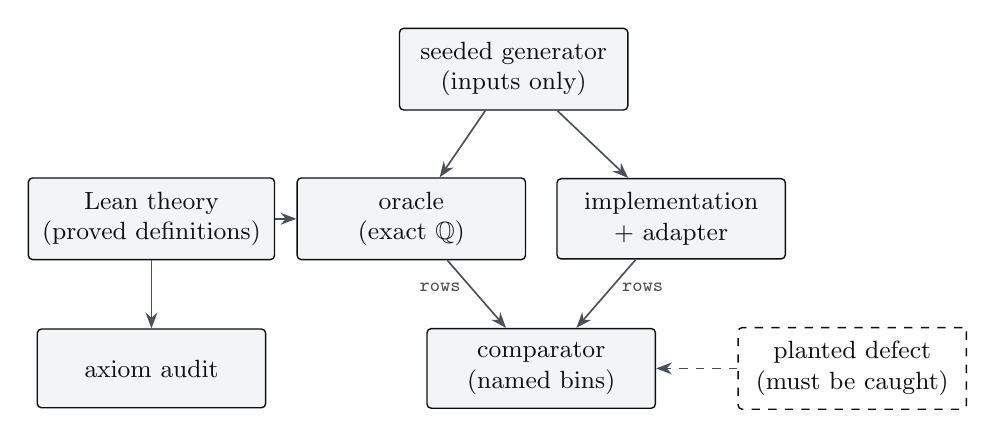
\begin{tikzpicture}[
  box/.style={draw=Ink, line width=0.5pt, fill=Surface, text=Ink, rounded corners=1.5pt,
    align=center, font=\small, inner sep=5pt, minimum height=10mm, minimum width=29mm},
  arr/.style={-{Stealth[length=2mm]}, line width=0.6pt, draw=InkMuted},
  lab/.style={font=\ttfamily\scriptsize, text=InkMuted}]
\node[box] (gen) at (4.6,1.9) {seeded generator\\(inputs only)};
\node[box] (theory) at (0,0) {Lean theory\\(proved definitions)};
\node[box] (oracle) at (3.3,0) {oracle\\(exact $\mathbb{Q}$)};
\node[box] (impl) at (6.6,0) {implementation\\+ adapter};
\node[box] (cmp) at (4.95,-1.9) {comparator\\(named bins)};
\node[box] (audit) at (0,-1.9) {axiom audit};
\node[box, dashed, fill=Background] (planted) at (8.9,-1.9) {planted defect\\(must be caught)};
\draw[arr] (gen) -- (oracle);
\draw[arr] (gen) -- (impl);
\draw[arr] (theory) -- (oracle);
\draw[arr] (theory) -- (audit);
\draw[arr] (oracle) -- node[left, lab, pos=0.4] {rows} (cmp);
\draw[arr] (impl) -- node[right, lab, pos=0.4] {rows} (cmp);
\draw[arr, dashed] (planted) -- (cmp);
\end{tikzpicture}
\caption{The measurement procedure. The generator never computes expected results;
those come only from the oracle.}
\label{fig:harness}
\end{figure}

The procedure follows \texttt{ledger-semantics} (\cref{fig:harness}). A seeded
generator writes case files containing inputs only. It favors the inputs where
implementations are known to have conventions: tied logits, words that are
themselves tokens, and merge tables with several splits of one string. A small
adapter per implementation runs the same cases and prints the oracle's row format.
The comparator places every case in exactly one named bin (agree, diverge, skipped
by either side, or missing), so nothing is dropped silently. Token rows are compared
as strings. Sampler rows require that a zero be matched by a zero and that nonzero
probabilities agree within $10^{-6}$, since llama.cpp stores logits in
\texttt{float32}. Each comparator is observed to fail: a planted defect, an adapter
that glues two tokens or one that inverts temperature, must be detected or the run
fails.

\paragraph{Tie divergences.} An implementation that keeps exactly $k$ tokens breaks
ties in its own order, which need not be the oracle's order by index. Every filter
treats tied tokens alike except for that choice, and tied tokens stay tied through
temperature and renormalization. Such an implementation must therefore agree with
the positional semantics up to a permutation of tied tokens. The harness checks
exactly this: the multiset of (logit, probability) pairs over the kept tokens must
equal that of the oracle's \texttt{q} rows. A divergence that fails this check is
reported as unexplained.

\begin{table}[t]
\centering\small
\caption{Measurements (\texttt{harness/run.sh 600}: four seeds of 600 cases each per
corpus). Lean 4.34.1, Mathlib v4.34.1, \texttt{tokenizers} 0.23.3, \texttt{tiktoken}
0.14.0, llama.cpp commit \texttt{a9d27ac} (2026-10-11).}
\label{tab:results}
\begin{tabularx}{\linewidth}{@{}>{\raggedright\arraybackslash}p{4.6cm}>{\raggedright\arraybackslash}X>{\raggedright\arraybackslash}X@{}}
\toprule
\qpth{Implementation} & \qpth{Compared against} & \qpth{Result}\\
\midrule
HF \texttt{tokenizers}, BPE, defaults & rule-rank BPE (\lean{bpe}) & 13{,}779 / 13{,}779 words identical\\
HF \texttt{tokenizers}, \lean{ignore_merges} & lookup, then rule-rank BPE & 13{,}779 / 13{,}779 identical\\
\texttt{tiktoken} & lookup, then concatenation-rank BPE & 13{,}779 / 13{,}779 identical\\
llama.cpp \lean{top_k}, \lean{top_p}, \lean{min_p}, \texttt{temp}, no ties & tie-keeping filters & 1{,}216 / 1{,}216 chains, $|\Delta p|\le5.1\times10^{-8}$\\
llama.cpp, with ties & tie-keeping, else positional & 939 + 245 / 1{,}184 chains; 0 unexplained\\
Planted defects (tokenizer, sampler) & --- & both detected\\
\bottomrule
\end{tabularx}
\end{table}

\Cref{tab:results} summarizes the results. Two findings came out of the
comparisons. First, \texttt{tiktoken} initially disagreed with the oracle's
concatenation-rank BPE on words that are themselves vocabulary tokens. The
disagreement was a convention, whole-word lookup. Following the
\texttt{ledger-semantics} rule that a divergence is either a defect in the
implementation or a convention the semantics has not yet recorded, we recorded it
as \lean{lookupFirst}, with its own theorems, after which agreement is exact.
Second, on the same random merge tables the two tokenizer libraries disagree with
each other on 439 of 13{,}779 words (3.2\%), and on 279 when Hugging Face uses
\lean{ignore_merges}. The oracle reproduces each library exactly, so every one of
these disagreements is predicted. \Cref{thm:bpeconv} states the condition under which
they cannot occur.

For sampling, llama.cpp agrees with the tie-keeping semantics on every tie-free
chain. On chains with ties, 245 of 1{,}184 diverge, and every one agrees with the
positional semantics up to a permutation of tied tokens. Some of these divergences
cascade: a tie cut by top-$k$ changes the renormalized masses that a later top-$p$
sees. A check that compared kept sets only after the fact would misclassify such
cases. Replaying the convention exactly classifies all of them.

% ===========================================================================
\section{Related work}

\paragraph{Formal methods for machine learning.} Most verification work on neural
networks proves properties of trained models, for example with SMT-based
methods~\cite{katz2017reluplex}. We verify the model-independent algorithms around
the model instead, and connect them to implementations through an oracle. The
denotational method follows Elliott~\cite{elliott2009denotational}. The use of a
proved semantics as a test oracle, the procedure of planted defects, and the
discipline of named skip bins follow \texttt{ledger-semantics}~\cite{ledgersemantics}.
Our category of finite stochastic maps is a special case of Fritz's Markov
categories~\cite{fritz2020markov}.

\paragraph{Tokenization.} Zouhar et al.\ give a formal analysis of BPE as an
optimization problem~\cite{zouhar2023bpe}. Gastaldi et al.\ treat tokenizers as
stochastic maps and study consistency of estimators~\cite{gastaldi2024foundations}.
Vieira et al.\ show how to turn token-level models into character-level
ones~\cite{vieira2024tokens}, which requires exactly the enumeration of
tokenizations we verify. Our no-compression theorem and the agreement criterion
between BPE conventions complement this work at the level of exact identities.

\paragraph{Decoding.} Top-$k$~\cite{fan2018hierarchical}, nucleus~\cite{holtzman2020curious}
and min-$p$~\cite{nguyen2025minp} sampling are usually specified by an algorithm over
sorted arrays, which leaves ties unspecified. \Cref{thm:topk} shows that this gap
cannot be closed by any symmetric rule. Speculative
sampling~\cite{leviathan2023speculative,chen2023speculative} is known to be lossless,
and its acceptance rate is the maximal-coupling bound~\cite{lindvall1992coupling}. Du et
al.\ characterize tightness measure-theoretically~\cite{du2023tight}. We give a
finite-depth statement and an explicit non-tight model.

\paragraph{Attention and inference systems.} Online softmax~\cite{milakov2018online}
underlies FlashAttention~\cite{dao2022flashattention} and its successors, and
KV caching is standard in serving systems~\cite{pope2023scaling,kwon2023vllm}. Our
contribution is the algebraic packaging, a commutative monoid with a free-monoid
homomorphism, and machine-checked proofs over arbitrary exponential characters.
Permutation equivariance of attention without positional encodings is
known~\cite{yun2020universal}.

\paragraph{Masked diffusion.} The time-independence of the optimal denoiser was
observed by Ou et al.~\cite{ou2025absorbing}, in the setting of
D3PM~\cite{austin2021d3pm}, MDLM~\cite{sahoo2024mdlm} and related
models~\cite{shi2024masked,nie2025llada}. We machine-check it, together with the
any-order chain rule and the inexactness of parallel unmasking.

% ===========================================================================
\section{Limitations}

Analysis on the reals enters only through exponential characters, and there is no
measure theory, so sampling and tightness are stated through finite quantities. The
oracle's temperature is restricted to $1/n$, which keeps softmax rational. The
theorems hold for every temperature, but the oracle cannot evaluate an irrational
softmax. Speculative decoding is proved for one drafted token. The sequence version
follows by induction and is not yet formalized. Nothing is proved about
floating-point arithmetic: implementations are compared with exact values within a
stated tolerance. A decision that lies exactly on a floating-point boundary could in
principle diverge, and none occurred in our runs. The diffusion theory covers
absorbing diffusion, not Gaussian diffusion. The chat protocol models tool calling in
its common request-and-result form, not any vendor's specification. The measurements
cover tokenizers and samplers; attention kernels, speculative decoders, chat
renderers and diffusion samplers are evaluated by the oracle but not yet compared
against implementations.

% ===========================================================================
\section{Conclusion}

The inference side of LLMs is small enough to be given a precise meaning and large
enough that its implementations disagree. A machine-checked semantics separates
what is meaning from what is convention. It proves which reorderings, cachings and
tilings are harmless, and it shows that some properties folklore expects, such as
symmetric exact top-$k$, compositional compressing tokenizers and unambiguous plain-text
templates, cannot exist. Connected to an exact oracle, the same definitions become
a test instrument. Every divergence it surfaces is either a defect in an
implementation or a convention that belongs in the semantics.

\paragraph{Availability.} The Lean development, oracle, harness, and recorded
measurement log accompany this paper.

\paragraph{Acknowledgments.} The structure of this work follows
\texttt{ledger-semantics} by John Wiegley. The formalization and harness were
developed with the assistance of an AI system (Claude, Anthropic).

% ===========================================================================
\begin{thebibliography}{99}\small

\bibitem{austin2021d3pm}
J.~Austin, D.~D. Johnson, J.~Ho, D.~Tarlow, and R.~van~den Berg.
\newblock Structured denoising diffusion models in discrete state-spaces.
\newblock In \emph{NeurIPS}, 2021.

\bibitem{chen2023speculative}
C.~Chen, S.~Borgeaud, G.~Irving, J.-B. Lespiau, L.~Sifre, and J.~Jumper.
\newblock Accelerating large language model decoding with speculative sampling.
\newblock arXiv:2302.01318, 2023.

\bibitem{dao2022flashattention}
T.~Dao, D.~Y. Fu, S.~Ermon, A.~Rudra, and C.~R{\'e}.
\newblock {FlashAttention}: Fast and memory-efficient exact attention with {IO}-awareness.
\newblock In \emph{NeurIPS}, 2022.

\bibitem{demoura2021lean4}
L.~de~Moura and S.~Ullrich.
\newblock The {Lean} 4 theorem prover and programming language.
\newblock In \emph{CADE-28}, 2021.

\bibitem{du2023tight}
L.~Du, L.~Torroba~Hennigen, T.~Pimentel, C.~Meister, J.~Eisner, and R.~Cotterell.
\newblock A measure-theoretic characterization of tight language models.
\newblock In \emph{ACL}, 2023.

\bibitem{elliott2009denotational}
C.~Elliott.
\newblock Denotational design with type class morphisms.
\newblock Technical Report 2009-01, LambdaPix, 2009.

\bibitem{fan2018hierarchical}
A.~Fan, M.~Lewis, and Y.~Dauphin.
\newblock Hierarchical neural story generation.
\newblock In \emph{ACL}, 2018.

\bibitem{fritz2020markov}
T.~Fritz.
\newblock A synthetic approach to {Markov} kernels, conditional independence and theorems on sufficient statistics.
\newblock \emph{Advances in Mathematics}, 370, 2020.

\bibitem{gastaldi2024foundations}
J.~L. Gastaldi, J.~Terilla, L.~Malagutti, B.~DuSell, T.~Vieira, and R.~Cotterell.
\newblock The foundations of tokenization: Statistical and computational concerns.
\newblock arXiv:2407.11606, 2024.

\bibitem{greshake2023injection}
K.~Greshake, S.~Abdelnabi, S.~Mishra, C.~Endres, T.~Holz, and M.~Fritz.
\newblock Not what you've signed up for: Compromising real-world {LLM}-integrated applications with indirect prompt injection.
\newblock In \emph{AISec}, 2023.

\bibitem{holtzman2020curious}
A.~Holtzman, J.~Buys, L.~Du, M.~Forbes, and Y.~Choi.
\newblock The curious case of neural text degeneration.
\newblock In \emph{ICLR}, 2020.

\bibitem{katz2017reluplex}
G.~Katz, C.~Barrett, D.~L. Dill, K.~Julian, and M.~J. Kochenderfer.
\newblock Reluplex: An efficient {SMT} solver for verifying deep neural networks.
\newblock In \emph{CAV}, 2017.

\bibitem{kwon2023vllm}
W.~Kwon, Z.~Li, S.~Zhuang, Y.~Sheng, L.~Zheng, C.~H. Yu, J.~E. Gonzalez, H.~Zhang, and I.~Stoica.
\newblock Efficient memory management for large language model serving with {PagedAttention}.
\newblock In \emph{SOSP}, 2023.

\bibitem{ledgersemantics}
J.~Wiegley.
\newblock ledger-semantics: Mathematical semantics of {Ledger}, the double-entry accounting tool.
\newblock \url{https://github.com/ledger/ledger-semantics}, 2026.

\bibitem{leviathan2023speculative}
Y.~Leviathan, M.~Kalman, and Y.~Matias.
\newblock Fast inference from transformers via speculative decoding.
\newblock In \emph{ICML}, 2023.

\bibitem{lindvall1992coupling}
T.~Lindvall.
\newblock \emph{Lectures on the Coupling Method}.
\newblock Wiley, 1992.

\bibitem{liu2023ring}
H.~Liu, M.~Zaharia, and P.~Abbeel.
\newblock Ring attention with blockwise transformers for near-infinite context.
\newblock arXiv:2310.01889, 2023.

\bibitem{mathlib2020}
The mathlib Community.
\newblock The {Lean} mathematical library.
\newblock In \emph{CPP}, 2020.

\bibitem{milakov2018online}
M.~Milakov and N.~Gimelshein.
\newblock Online normalizer calculation for softmax.
\newblock arXiv:1805.02867, 2018.

\bibitem{nguyen2025minp}
M.~N. Nguyen, A.~Baker, C.~Neo, A.~Roush, A.~Kirsch, and R.~Shwartz-Ziv.
\newblock Turning up the heat: Min-p sampling for creative and coherent {LLM} outputs.
\newblock In \emph{ICLR}, 2025.

\bibitem{nie2025llada}
S.~Nie, F.~Zhu, Z.~You, X.~Zhang, J.~Ou, J.~Hu, J.~Zhou, Y.~Lin, J.-R. Wen, and C.~Li.
\newblock Large language diffusion models.
\newblock arXiv:2502.09992, 2025.

\bibitem{ou2025absorbing}
J.~Ou, S.~Nie, K.~Xue, F.~Zhu, J.~Sun, Z.~Li, and C.~Li.
\newblock Your absorbing discrete diffusion secretly models the conditional distributions of clean data.
\newblock In \emph{ICLR}, 2025.

\bibitem{pope2023scaling}
R.~Pope, S.~Douglas, A.~Chowdhery, J.~Devlin, J.~Bradbury, J.~Heek, K.~Xiao, S.~Agrawal, and J.~Dean.
\newblock Efficiently scaling transformer inference.
\newblock In \emph{MLSys}, 2023.

\bibitem{rabe2021selfattention}
M.~N. Rabe and C.~Staats.
\newblock Self-attention does not need {$O(n^2)$} memory.
\newblock arXiv:2112.05682, 2021.

\bibitem{radford2019gpt2}
A.~Radford, J.~Wu, R.~Child, D.~Luan, D.~Amodei, and I.~Sutskever.
\newblock Language models are unsupervised multitask learners.
\newblock OpenAI technical report, 2019.

\bibitem{sahoo2024mdlm}
S.~S. Sahoo, M.~Arriola, Y.~Schiff, A.~Gokaslan, E.~Marroquin, J.~T. Chiu, A.~Rush, and V.~Kuleshov.
\newblock Simple and effective masked diffusion language models.
\newblock In \emph{NeurIPS}, 2024.

\bibitem{sennrich2016bpe}
R.~Sennrich, B.~Haddow, and A.~Birch.
\newblock Neural machine translation of rare words with subword units.
\newblock In \emph{ACL}, 2016.

\bibitem{shi2024masked}
J.~Shi, K.~Han, Z.~Wang, A.~Doucet, and M.~K. Titsias.
\newblock Simplified and generalized masked diffusion for discrete data.
\newblock In \emph{NeurIPS}, 2024.

\bibitem{vieira2024tokens}
T.~Vieira, B.~LeBrun, M.~Giulianelli, J.~L. Gastaldi, B.~DuSell, J.~Terilla, T.~J. O'Donnell, and R.~Cotterell.
\newblock From language models over tokens to language models over characters.
\newblock arXiv:2412.03719, 2024.

\bibitem{wolf2020transformers}
T.~Wolf et~al.
\newblock Transformers: State-of-the-art natural language processing.
\newblock In \emph{EMNLP: System Demonstrations}, 2020.

\bibitem{xiao2024sinks}
G.~Xiao, Y.~Tian, B.~Chen, S.~Han, and M.~Lewis.
\newblock Efficient streaming language models with attention sinks.
\newblock In \emph{ICLR}, 2024.

\bibitem{yun2020universal}
C.~Yun, S.~Bhojanapalli, A.~S. Rawat, S.~J. Reddi, and S.~Kumar.
\newblock Are transformers universal approximators of sequence-to-sequence functions?
\newblock In \emph{ICLR}, 2020.

\bibitem{zouhar2023bpe}
V.~Zouhar, C.~Meister, J.~L. Gastaldi, L.~Du, T.~Vieira, M.~Sachan, and R.~Cotterell.
\newblock A formal perspective on byte-pair encoding.
\newblock In \emph{Findings of ACL}, 2023.

\end{thebibliography}

\end{document}
"
% ---------------------------------------------------------------------------
\documentclass[10pt]{article}

\newif\ifqptdark
\qptdarkfalse   % print edition (light). \qptdarktrue gives the dark screen edition.
\ifdefined\qptdarkedition\qptdarktrue\fi  % or: xelatex "\def\qptdarkedition{}% !TeX program = xelatex
% ---------------------------------------------------------------------------
%  A Machine-Checked Semantics of LLM Inference
%  Daniel Arango Sohm, Universidad EAFIT
%
%  Typeset in the QPT visual design system:
%    * neutral-first: Ink on Background carries the document;
%    * paradigm colours are semantic only. This paper belongs to none of the
%      five paradigms, so no paradigm colour appears in its content; the
%      colours appear only in the QPT mark itself;
%    * no gradients;
%    * Space Grotesk for display, Inter for body text, IBM Plex Mono for
%      technical, numeric, label, code and proof-oriented content.
%
%  Compile with:  xelatex llm-semantics-qpt.tex   (twice, for references)
%  Dark screen edition: set \qptdarktrue below, or run
%    xelatex -jobname=llm-semantics-qpt-dark "\def\qptdarkedition{}\input{llm-semantics-qpt}"
% ---------------------------------------------------------------------------
\documentclass[10pt]{article}

\newif\ifqptdark
\qptdarkfalse   % print edition (light). \qptdarktrue gives the dark screen edition.
\ifdefined\qptdarkedition\qptdarktrue\fi  % or: xelatex "\def\qptdarkedition{}\input{llm-semantics-qpt}"

\usepackage[a4paper,textwidth=15.4cm,textheight=23.6cm,top=3.0cm,headsep=0.9cm,footskip=1.2cm]{geometry}
\usepackage{amsmath,amssymb,amsthm,mathtools}
\usepackage{fontspec}
\usepackage{booktabs,tabularx,array}
\usepackage[protrusion=true,expansion=false]{microtype}
\usepackage[table]{xcolor}
\usepackage{graphicx}
\usepackage{fvextra}
\usepackage{enumitem}
\usepackage{caption}
\usepackage{titlesec}
\usepackage{fancyhdr}
\usepackage[most]{tcolorbox}
\usepackage{tikz}
\usetikzlibrary{arrows.meta}
\usepackage{hyperref}
\usepackage[nameinlink,capitalise]{cleveref}

% ---------------------------------------------------------------------------
%  Colour tokens
% ---------------------------------------------------------------------------
% Neutral foundation. Ink and Background invert between the two editions.
\ifqptdark
  \definecolor{Background}{HTML}{0B0C0E}
  \definecolor{Surface}{HTML}{16181B}
  \definecolor{Border}{HTML}{2B2E33}
  \definecolor{Ink}{HTML}{EDEEF0}
  \definecolor{InkMuted}{HTML}{A9AEB6}
  \definecolor{InkFaint}{HTML}{5A5F67}   % decoration only, never meaningful text
\else
  \definecolor{Background}{HTML}{FFFFFF}
  \definecolor{Surface}{HTML}{F3F4F5}
  \definecolor{Border}{HTML}{DADDE1}
  \definecolor{Ink}{HTML}{0E0F11}
  \definecolor{InkMuted}{HTML}{4B4F57}
  \definecolor{InkFaint}{HTML}{A3A7AE}   % decoration only, never meaningful text
\fi
% Paradigm colours: fixed in both editions, semantic only.
\definecolor{Quantum}{HTML}{5BAD1E}
\definecolor{Photonic}{HTML}{F0AB00}
\definecolor{Thermodynamic}{HTML}{E8690A}
\definecolor{Ternary}{HTML}{8A8A8A}
\definecolor{Bio}{HTML}{1AAB7C}

\ifqptdark\pagecolor{Background}\fi

% ---------------------------------------------------------------------------
%  Typography
% ---------------------------------------------------------------------------
\setmainfont{Inter}[
  Path=fonts/, Extension=.otf, Scale=0.94,
  UprightFont=*-Regular, ItalicFont=*-Italic,
  BoldFont=*-SemiBold, BoldItalicFont=*-SemiBoldItalic]
\setmonofont{IBMPlexMono}[
  Path=fonts/, Extension=.ttf, Scale=MatchLowercase,
  UprightFont=*-Regular, ItalicFont=*-Italic, BoldFont=*-SemiBold]
\newfontfamily\qptdisplay{SpaceGrotesk}[
  Path=fonts/, Extension=.otf, UprightFont=*-Medium, BoldFont=*-Bold]
\newfontfamily\qptdisplaylight{SpaceGrotesk}[
  Path=fonts/, Extension=.otf, UprightFont=*-Regular]
\newfontfamily\qptlabelfont{IBMPlexMono}[
  Path=fonts/, Extension=.ttf, Scale=MatchLowercase, UprightFont=*-Medium,
  LetterSpace=6]
\setsansfont{Inter}[
  Path=fonts/, Extension=.otf, Scale=0.94,
  UprightFont=*-Regular, ItalicFont=*-Italic,
  BoldFont=*-SemiBold, BoldItalicFont=*-SemiBoldItalic]
\linespread{1.16}
\setlength{\emergencystretch}{2.5em}
\AtBeginDocument{\raggedright\setlength{\parindent}{0pt}}
\setlength{\parindent}{0pt}
\setlength{\parskip}{0.55em}

% A label: IBM Plex Mono, upper case, tracked.
\newcommand{\qptlabel}[1]{{\qptlabelfont\footnotesize\MakeUppercase{#1}}}
% Technical names (Lean declarations, files) in IBM Plex Mono.
\newcommand{\lean}[1]{\texttt{\detokenize{#1}}}
\newcommand{\leanref}[1]{\par\smallskip\noindent
  {\ttfamily\footnotesize\upshape\raggedright\color{InkMuted}LEAN\enspace #1\par}}

% Ink is the normal colour everywhere, including floats, heads and footnotes.
\makeatletter
\AtBeginDocument{\color{Ink}\global\let\default@color\current@color}
\makeatother

% ---------------------------------------------------------------------------
%  Mathematical notation
% ---------------------------------------------------------------------------
\newcommand{\K}{\Bbbk}
\newcommand{\Dist}{\mathrm{Dist}}
\newcommand{\restr}[2]{#1|_{#2}}
\newcommand{\topk}{\mathrm{TopK}}
\newcommand{\topp}{\mathrm{TopP}}
\newcommand{\minp}{\mathrm{MinP}}
\newcommand{\sharpen}{\mathrm{sharpen}}
\newcommand{\abv}{\mathrm{above}}
\newcommand{\tv}{\mathrm{tv}}
\newcommand{\dec}{\mathrm{dec}}
\newcommand{\enc}{\mathrm{enc}}
\newcommand{\softmax}{\mathrm{softmax}}
\newcommand{\attend}{\mathrm{attend}}
\newcommand{\Iv}[1]{[\![#1]\!]}
\newcommand{\Mask}{\bot}

% ---------------------------------------------------------------------------
%  Headings: section numbers as labels, titles in Space Grotesk
% ---------------------------------------------------------------------------
\makeatletter
\newcommand{\qptsecnum}[1]{{\qptlabelfont\small\color{InkMuted}\two@digits{#1}}}
\makeatother
\titleformat{\section}
  {\qptdisplay\fontsize{14.5}{18}\selectfont\color{Ink}}
  {\qptsecnum{\value{section}}}{0.9em}{}
\titleformat{name=\section,numberless}
  {\qptdisplay\fontsize{14.5}{18}\selectfont\color{Ink}}{}{0pt}{}
\titlespacing*{\section}{0pt}{1.9em}{0.7em}
\titleformat{\paragraph}[runin]
  {\qptdisplay\normalsize\color{Ink}}{}{0pt}{}
\titlespacing*{\paragraph}{0pt}{0.9em}{0.6em}

% ---------------------------------------------------------------------------
%  Statements
% ---------------------------------------------------------------------------
\newtheoremstyle{qpt}
  {0.9em}{0.9em}
  {\normalfont}{}
  {\qptlabelfont\footnotesize}{}
  {\newline}
  {\MakeUppercase{\thmname{#1}\thmnumber{~#2}}%
   \thmnote{\enspace{\qptdisplay\normalsize\color{Ink}#3}}}
\theoremstyle{qpt}
\newtheorem{theorem}{Theorem}
\newtheorem{proposition}[theorem]{Proposition}
\newtheorem{corollary}[theorem]{Corollary}
\newtheorem{lemma}[theorem]{Lemma}
\newtheorem{definition}[theorem]{Definition}
\newtheorem{remark}[theorem]{Remark}

% Proofs: a tracked label and a neutral end mark.
\makeatletter
\renewcommand{\qedsymbol}{{\color{InkMuted}\rule{0.5em}{0.5em}}}
\renewenvironment{proof}[1][Proof]{\par\pushQED{\qed}\normalfont\topsep0.5em\relax
  \trivlist\item[\hskip\labelsep\qptlabel{#1}\hspace{0.6em}]\ignorespaces}
  {\popQED\endtrivlist\@endpefalse}
\makeatother

% ---------------------------------------------------------------------------
%  Code: IBM Plex Mono on a neutral surface, with a hairline on the left
% ---------------------------------------------------------------------------
\tcbset{colupper=Ink, collower=Ink}
\tcbset{qptcode/.style={enhanced, colback=Surface, colframe=Surface,
  boxrule=0pt, arc=0pt, left=9pt, right=8pt, top=5pt, bottom=5pt,
  borderline west={1.2pt}{0pt}{InkFaint}, before skip=0.7em, after skip=0.7em}}
\newenvironment{leancode}
  {\VerbatimEnvironment\begin{tcolorbox}[qptcode]%
   \begin{Verbatim}[fontsize=\small,commandchars=\\\{\},
     codes={\catcode`\$=3\catcode`\^=7},formatcom=\color{Ink}]}
  {\end{Verbatim}\end{tcolorbox}}
\newenvironment{casecode}
  {\VerbatimEnvironment\begin{tcolorbox}[qptcode,before skip=0pt,after skip=0pt]%
   \begin{Verbatim}[fontsize=\footnotesize,formatcom=\color{Ink}]}
  {\end{Verbatim}\end{tcolorbox}}

% ---------------------------------------------------------------------------
%  Floats, tables, captions
% ---------------------------------------------------------------------------
\DeclareCaptionLabelFormat{qpt}{\qptlabel{#1~#2}}
\DeclareCaptionLabelSeparator{qptsep}{\quad}
\captionsetup{labelformat=qpt, labelsep=qptsep, font={small,color=Ink},
  justification=raggedright, singlelinecheck=false, skip=6pt}
\newcommand{\qpth}[1]{\qptlabel{#1}}
\arrayrulecolor{Ink}
\setlength{\heavyrulewidth}{0.7pt}
\setlength{\lightrulewidth}{0.35pt}
\renewcommand{\arraystretch}{1.22}

% ---------------------------------------------------------------------------
%  Running heads
% ---------------------------------------------------------------------------
\pagestyle{fancy}
\fancyhf{}
\fancyhead[L]{{\color{Ink}\qptlabel{Machine-checked semantics of LLM inference}}}
\fancyhead[R]{{\color{Ink}\qptlabel{D. Arango Sohm}}}
\fancyfoot[R]{{\ttfamily\small\color{InkMuted}\thepage}}
\renewcommand{\headrule}{{\color{Border}\hrule height 0.4pt}\vspace{-0.4pt}}
\renewcommand{\headrulewidth}{0.4pt}
\fancypagestyle{qptfirst}{\fancyhf{}%
  \fancyfoot[R]{{\ttfamily\small\color{InkMuted}\thepage}}%
  \renewcommand{\headrulewidth}{0pt}\renewcommand{\headrule}{}}

% ---------------------------------------------------------------------------
%  Links and references: neutral, never accent-coloured text
% ---------------------------------------------------------------------------
\hypersetup{colorlinks=true, linkcolor=Ink, citecolor=Ink, urlcolor=Ink,
  pdftitle={A Machine-Checked Semantics of LLM Inference},
  pdfauthor={Daniel Arango Sohm},
  pdfsubject={Formal semantics of large language model inference in Lean 4},
  pdfkeywords={Lean 4, Mathlib, formal verification, LLM inference, sampling,
    tokenization, attention, speculative decoding, diffusion language models}}
\makeatletter
\renewcommand{\@biblabel}[1]{{\ttfamily\color{InkMuted}[#1]}}
\renewcommand{\@cite}[2]{{\ttfamily[#1\if@tempswa, #2\fi]}}
\makeatother
\renewcommand{\refname}{References}

\setlist{itemsep=2pt, topsep=4pt}
\setlist[itemize]{label={\color{InkMuted}\textbullet}}

\begin{document}
\thispagestyle{qptfirst}

% ----------------------------------------------------------------- masthead
\noindent
\begin{minipage}[c]{0.5\linewidth}
  \includegraphics[height=1.9cm]{qpt-logo.png}
\end{minipage}%
\begin{minipage}[c]{0.5\linewidth}\raggedleft
  \qptlabel{Preprint}\\[2pt]
  \qptlabel{October 2026}
\end{minipage}

\vspace{1.6em}
{\color{Border}\rule{\linewidth}{0.4pt}}
\vspace{1.1em}

{\qptdisplay\fontsize{25}{29.5}\selectfont\color{Ink}
A Machine-Checked Semantics\\ of LLM Inference\par}
\vspace{0.55em}
{\qptdisplaylight\fontsize{13}{17}\selectfont\color{InkMuted}
Sampling, Attention, Tokenization, Chat, Decoding,\\ and Diffusion in Lean~4\par}

\vspace{1.5em}
{\large\bfseries Daniel Arango Sohm}\par
\vspace{0.15em}
{\color{InkMuted}Universidad EAFIT, Medellín, Colombia\\
Former member of the QPT team}\par

\vspace{1.4em}
% ----------------------------------------------------------------- abstract
\begin{tcolorbox}[enhanced, colback=Surface, colframe=Surface, colupper=Ink, boxrule=0pt,
  arc=0pt, left=12pt, right=12pt, top=9pt, bottom=10pt]
\qptlabel{Abstract}\par\vspace{0.35em}
{\small
The inference side of a large language model is a stack of small algorithms:
tokenizers, attention kernels, key--value caches, sampling filters, speculative
decoders, chat templates, and diffusion samplers. Each has several independent
implementations, and those implementations are usually tested against one another
rather than against a definition. We give these components a single mathematical
semantics, formalized in Lean~4 against Mathlib. The development comprises about
4{,}600 lines and 270 named theorems, and every declaration depends only on Lean's
three standard axioms. It proves the exact algebra of sampling filters, the
losslessness and optimality of speculative sampling, and the correctness of
key--value caching and of FlashAttention-style online softmax as a commutative
monoid. It proves that byte-pair encoding is lossless under every merge priority,
together with a decidable criterion for when the Hugging Face and \texttt{tiktoken}
conventions agree, a protocol checker for tool calls, and the time-independence of
the masked-diffusion denoiser. It also proves six negative results. No sampling
rule that treats tokens symmetrically can always keep exactly $k$ tokens. No
tokenizer that compresses can respect concatenation. Every chat template that writes
its role markers in the content alphabet is ambiguous. No transformer without
positional information can copy a fixed position. An autoregressive model need not
define a distribution over strings. Parallel unmasking in diffusion is inexact.
From the same definitions we build an executable oracle that evaluates test cases in
exact rational arithmetic, and a harness that measures implementations against it.
On 2{,}400 random merge tables, Hugging Face \texttt{tokenizers} and
\texttt{tiktoken} each agree with the oracle on all 13{,}779 test words, while
disagreeing with each other on 3.2\% of them. On 2{,}400 random sampler chains,
every divergence of llama.cpp from the tie-keeping semantics is accounted for
exactly by the positional semantics that the impossibility theorem forces.
\par}
\end{tcolorbox}

\vspace{0.3em}
\noindent\qptlabel{Keywords}\enspace{\small Lean~4 · Mathlib · formal verification ·
LLM inference · sampling · tokenization · attention · speculative decoding ·
diffusion language models}

\vspace{0.4em}
{\color{Border}\rule{\linewidth}{0.4pt}}

% ===========================================================================
\section{Introduction}

A deployed language model is a function from parameters and a context to a
distribution over tokens. Turning that distribution into text requires more
machinery. A tokenizer maps strings to token sequences. Attention kernels compute
the model's reads over a cached context. A chain of sampling filters reshapes the
next-token distribution. A speculative decoder may verify drafted tokens, a chat
template linearizes a conversation, and a diffusion sampler may unmask several
positions at once. Each of these components exists in many implementations, such as
Hugging Face \texttt{transformers} and \texttt{tokenizers}~\cite{wolf2020transformers},
\texttt{tiktoken}, vLLM~\cite{kwon2023vllm}, and llama.cpp. Their tests mostly
compare one implementation with another, or with remembered behavior.

This paper follows a different discipline, \emph{denotational design}~\cite{elliott2009denotational}.
One first says precisely what a thing means, then requires every operation to
preserve that meaning, and lets the implementation be whatever the equations force
it to be. The approach is that of \texttt{ledger-semantics}~\cite{ledgersemantics},
which formalizes double-entry accounting in Lean and uses the result as a test oracle
for the C++ Ledger program. We apply it to LLM inference. A sampling filter means
conditioning a distribution on a set. A KV-cached decoder means causal attention over
the whole prefix. A FlashAttention kernel means a softmax-weighted average. A chat
template means an injective encoding of a transcript. The theorems state when an
implementation preserves that meaning, and several of them state that no
implementation can.

\paragraph{Contributions.}
\begin{itemize}[leftmargin=*,itemsep=2pt]
\item A Lean~4 formalization against Mathlib~\cite{mathlib2020,demoura2021lean4}
  of sampling, speculative decoding, softmax and attention, tokenization, chat
  transcripts, autoregressive decoding, and masked diffusion
  (\cref{sec:foundations,sec:sampling,sec:spec,sec:attention,sec:tokenization,sec:chat,sec:decoding,sec:diffusion}).
  All definitions are stated over an arbitrary linearly ordered field, so one proof
  covers the real numbers of the literature and the exact rationals of the oracle.
\item Positive results in a common framework. They include the algebra of
  sampling filters, the optimality of speculative sampling, an online-softmax
  commutative monoid, a generic correctness theorem for BPE with a decidable
  agreement criterion between the two conventions in use, a protocol checker for
  tool calls, and the any-order chain rule for masked diffusion.
\item Six negative results that explain design constraints visible across
  implementations (\cref{sec:negative}).
\item An executable oracle that evaluates case files under the proved
  definitions in exact arithmetic, and a measurement of Hugging Face
  \texttt{tokenizers}, \texttt{tiktoken}, and llama.cpp against it (\cref{sec:oracle,sec:measure}).
\end{itemize}

Several of the positive results are known: losslessness of speculative
sampling~\cite{leviathan2023speculative,chen2023speculative}, correctness of online
softmax~\cite{milakov2018online,dao2022flashattention}, time-independence of the
absorbing-diffusion posterior~\cite{ou2025absorbing}, and the role of permutation
equivariance~\cite{yun2020universal}. Our contribution for these is a machine-checked
statement in one framework, connected to an oracle. To our knowledge the
following are not stated elsewhere in the form given here: the impossibility of
symmetric exact top-$k$ and nucleus selection, the no-compression theorem for
homomorphic tokenizers, the ambiguity of every in-band chat template, and the
decidable agreement criterion between merge-rule and concatenation-rank BPE.

% ===========================================================================
\section{Method and trust base}\label{sec:method}

The development is a Lean~4 library (Lean 4.34.1, Mathlib v4.34.1) of eleven
theory modules and two executable modules (\cref{tab:modules}). It is built with
warnings promoted to errors, so an unproved theorem (\lean{sorry}) fails the build.
A separate audit program walks every declaration in the library, 853 in all, and
fails unless each depends only on propositional extensionality, the axiom of choice,
and quotient soundness. The audit has been observed to fail: a planted proof by
\lean{native_decide}, which introduces an auxiliary axiom trusting compiled code, is
rejected. The warnings-as-errors build alone does not catch it. Concrete
counterexamples are therefore proved by \lean{decide}, whose certificate the kernel
checks by evaluation.

\begin{table}[t]
\centering\small
\caption{Modules of the development. Lines and named theorems and lemmas per module.}
\label{tab:modules}
\begin{tabularx}{\linewidth}{@{}l>{\raggedright\arraybackslash}X>{\ttfamily}r>{\ttfamily}r@{}}
\toprule
\qpth{Module} & \qpth{Content} & \qpth{Lines} & \qpth{Thms} \\
\midrule
\lean{Dist} & finite distributions, conditioning, total variation, $\mathsf{FinStoch}$ & 383 & 34\\
\lean{Sampling} & top-$k$, top-$p$, min-$p$, temperature, ties, inverse CDF & 732 & 46\\
\lean{Counterexamples} & kernel-checked failures of sampler laws & 52 & 4\\
\lean{Speculative} & speculative sampling, couplings & 194 & 17\\
\lean{Softmax} & exponential characters, masking, temperature & 220 & 23\\
\lean{Attention} & equivariance, causality, KV cache, online softmax & 573 & 38\\
\lean{Real} & $\exp$ as a character; textbook restatements & 51 & 4\\
\lean{Tokenization} & free-monoid decoding, BPE conventions, enumeration & 860 & 49\\
\lean{Chat} & tool-call protocol, rendering & 440 & 21\\
\lean{Decoding} & mass conservation, tightness, greedy decoding & 245 & 15\\
\lean{Diffusion} & masked diffusion, posterior, chain rule & 379 & 18\\
\lean{Oracle}, \lean{Driver} & case parsing and exact evaluation & 465 & 1\\
\midrule
Total & & 4{,}594 & 270\\
\bottomrule
\end{tabularx}
\end{table}

\paragraph{Numbers.} Every probability lives in an arbitrary field $\K$ with a
compatible linear order (\lean{[Field K] [LinearOrder K] [IsStrictOrderedRing K]}).
The oracle instantiates $\K=\mathbb{Q}$, so its arithmetic is exact. The analytic
statements instantiate $\K=\mathbb{R}$. No measure theory is used. Sampling is made
precise through interval statements (\cref{thm:invcdf}), and tightness through
masses at finite depth (\cref{sec:decoding}).

% ===========================================================================
\section{Foundations}\label{sec:foundations}

\begin{definition}[Finite distribution]
For a finite type $\alpha$, $\Dist_\K(\alpha)$ is the type of functions
$p:\alpha\to\K$ with $p(a)\ge 0$ for all $a$ and $\sum_a p(a)=1$.
\leanref{\lean{Dist}}
\end{definition}

\begin{leancode}
structure Dist ($\K$ : Type u) [Field $\K$] [LinearOrder $\K$] [IsStrictOrderedRing $\K$]
    ($\alpha$ : Type v) [Fintype $\alpha$] where
  prob : $\alpha$ $\to$ $\K$
  nonneg : $\forall$ a, 0 $\le$ prob a
  sum_eq_one : $\sum$ a, prob a = 1
\end{leancode}

The single operation through which masks, filters and grammar constraints act is
conditioning. For $S\subseteq\alpha$ with $p(S)>0$, write
$\restr{p}{S}(a)=\Iv{a\in S}\,p(a)/p(S)$ (\lean{Dist.restrict}).

\begin{lemma}[Conditioning]\label{lem:restrict}
$\restr{(\restr{p}{S})}{T}=\restr{p}{S\cap T}$ whenever the masses involved are
positive. Moreover $\restr{p}{S}=\restr{p}{S'}$ whenever $S$ and $S'$ contain the same
outcomes of positive probability.
\leanref{\lean{restrict_restrict}, \lean{restrict_congr}}
\end{lemma}

The finite distribution monad (point masses and \lean{bind}) satisfies the monad
laws. Finite types and stochastic maps $\alpha\to\Dist_\K(\beta)$ form a category
$\mathsf{FinStoch}_\K$, given as an instance of Mathlib's \lean{Category} whose
composition is Kleisli composition (\lean{FinStoch.category}). Total variation is
$\tv(p,q)=\sum_a\max(0,p(a)-q(a))$. We prove
$\tv(p,q)=\tfrac12\sum_a|p(a)-q(a)|$, $\sum_a\min(p(a),q(a))=1-\tv(p,q)$, and
$\tv(p,q)=0\iff p=q$.

% ===========================================================================
\section{Sampling}\label{sec:sampling}

Let $V$ be a finite vocabulary and $p:V\to\K$. Write
$\abv_p(v)=\{u: p(v)<p(u)\}$ for the tokens strictly preferred to $v$. The three
standard filters keep the sets
\begin{gather*}
\topk_k(p)=\{v: |\abv_p(v)|<k\},\qquad
\minp_m(p)=\{v:\forall u,\; m\,p(u)\le p(v)\},\\
\topp_P(p)=\Bigl\{v: \textstyle\sum_{u\in\abv_p(v)}p(u)<P\Bigr\},
\end{gather*}
and the filtered distribution is the conditioning $\restr{p}{S}$ on the kept set
$S$. For distinct probabilities, $\topp_P$ is the usual rule ``sort in descending
order and keep the shortest prefix whose mass reaches $P$''. With ties, all three
keep every tied token. Temperature $1/n$ is
$\sharpen_n(p)(v)=p(v)^n/\sum_u p(u)^n$, which stays inside $\mathbb{Q}$. In
\cref{sec:attention} we show that it equals $\softmax(n\cdot z)$ when
$p=\softmax(z)$. Every kept set contains a most probable token, provided $k\ge1$,
$P>0$ and $m\le1$, so no filter can produce an empty distribution.

\begin{theorem}[Sampler algebra]\label{thm:algebra}
For $k,k'\ge1$, $m,m'\le1$ and $n\ge1$, and writing filters in the order they are
applied,
\begin{enumerate}[label=(\roman*),itemsep=1pt]
\item top-$k$ then top-$k'$ equals top-$\min(k,k')$;
\item min-$m$ then min-$m'$ equals min-$\max(m,m')$; in particular both filters are idempotent;
\item top-$k$ and min-$m$ commute;
\item top-$k$ and temperature $1/n$ commute.
\end{enumerate}
\leanref{\lean{topK_topK}, \lean{minP_minP}, \lean{topK_minP_comm}, \lean{topK_sharpen_comm}}
\end{theorem}

\begin{proof}[Proof sketch]
All three kept sets are \emph{upward closed}: if $v$ is kept and $p(v)<p(u)$, then
$u$ is kept. Conditioning on an upward-closed set $S$ leaves $\abv(v)$ unchanged for
$v\in S$ (\lean{above_restrict}), and min-$p$ is insensitive to conditioning on a set
that contains a maximizer (\lean{minP_restrict_iff}). Each identity then reduces,
through \cref{lem:restrict}, to an equality of kept sets. For (iv), $x\mapsto x^n$
is strictly increasing on $[0,\infty)$, and top-$k$ depends only on the order of the
scores (\lean{topKSet_congr}).
\end{proof}

The laws one might expect beyond \cref{thm:algebra} are false. With
$p_0=(\tfrac12,\tfrac3{10},\tfrac15)$, the kernel evaluates the following
(\lean{Counterexamples}).

\begin{proposition}[Failed laws]\label{prop:counter}
\leavevmode\vspace{-0.5\baselineskip}
\begin{enumerate}[label=(\roman*),itemsep=1pt]
\item Top-$p$ is not idempotent: one pass of $\topp_{3/5}$ gives token~1 the probability $\tfrac38$, and a second pass gives it~$0$.
\item Top-$p$ does not commute with top-$k$: top-$p$ then top-2 leaves token~1 at $\tfrac38$, while top-2 then top-$p$ removes it.
\item Top-$p$ does not commute with temperature $\tfrac12$: token~1 ends at $\tfrac9{34}$ in one order and at $0$ in the other.
\item Min-$p$ ($m=\tfrac12$) does not commute with temperature $\tfrac12$, with the same numbers.
\end{enumerate}
\end{proposition}

A sampler chain may therefore reorder top-$k$, min-$p$ and temperature only as
\cref{thm:algebra} allows, and may not move top-$p$ at all.

\paragraph{Ties.} Implementations differ on ties, and the difference is forced.
Call a selection rule $\mathrm{sel}:(V\to\K)\to\mathcal{P}(V)$ \emph{equivariant} if
$\mathrm{sel}(p\circ\sigma^{-1})=\sigma[\mathrm{sel}(p)]$ for every permutation
$\sigma$ of $V$, that is, if relabeling the tokens relabels the output.

\begin{theorem}[No symmetric exact top-$k$]\label{thm:topk}
Let $0<k<|V|$. No equivariant selection rule satisfies $|\mathrm{sel}(p)|=k$ for
every distribution $p$.
\leanref{\lean{no_equivariant_exact_topK}}
\end{theorem}
\begin{proof}
On the uniform distribution $u$ we have $u\circ\sigma^{-1}=u$ for every $\sigma$, so
$\mathrm{sel}(u)$ is invariant under all permutations. If it contains some $v$, then
for any $w$ the transposition $(v\,w)$ maps $v$ to $w$, so it contains $w$ too.
Hence $\mathrm{sel}(u)$ is either empty or all of $V$, and neither has $k$ elements.
\end{proof}

\begin{leancode}
theorem no_equivariant_exact_topK [DecidableEq V] \char123{}k : $\mathbb{N}$\char125{}
    (hk0 : 0 < k) (hkn : k < Fintype.card V)
    (sel : (V $\to$ $\K$) $\to$ Finset V) (hsel : Equivariant sel) :
    $\neg$ $\forall$ d : Dist $\K$ V, (sel d.prob).card = k
\end{leancode}

\begin{theorem}[No symmetric smallest nucleus]
Let $V$ be nonempty and $0<P\le1-1/|V|$. No equivariant rule returns, for every
distribution, a set of minimum cardinality among those of mass at least~$P$.
\leanref{\lean{no_equivariant_exact_nucleus}}
\end{theorem}

The tie-keeping filters are equivariant (\lean{topKSet_equivariant}). The other
option is to break ties by position. Define $u\prec_p v$ if $p(u)>p(v)$, or if
$p(u)=p(v)$ and $u<v$, and let the positional filters count predecessors under
$\prec_p$ instead of $\abv_p$ (\lean{Dist.topKPos}, \lean{Dist.topPPos}).

\begin{theorem}[Positional tie-breaking]
Positional top-$k$ keeps exactly $\min(k,|V|)$ tokens. If $p$ is injective, the
positional and tie-keeping filters coincide. For $0<k<|V|$, positional top-$k$ is
not equivariant.
\leanref{\lean{card_topKPosSet}, \lean{topKPosSet_eq_of_injective}, \lean{topPPosSet_eq_of_injective}, \lean{topKPosSet_not_equivariant}}
\end{theorem}

An implementation must therefore choose between keeping exactly $k$ tokens and
treating tokens symmetrically. Hugging Face \texttt{transformers} (read from the
source of version 5.19.0) keeps ties in top-$k$, since it removes only scores
strictly below the $k$-th largest, but breaks them by sort position in top-$p$.
llama.cpp breaks ties by position in both, as measured in \cref{sec:measure}.

\begin{theorem}[Inverse-CDF sampling]\label{thm:invcdf}
Let $F(i)=\sum_{j<i}p(j)$ on $V=\{0,\dots,n-1\}$ and let $\iota(u)$ be the least $i$
with $u<F(i+1)$. For $0\le u<1$, $\iota(u)=i\iff F(i)\le u<F(i+1)$, and
$F(i+1)-F(i)=p(i)$. A uniform $u$ therefore selects $i$ with probability $p(i)$.
\leanref{\lean{invCdf_eq_iff}, \lean{cdf_interval_length}}
\end{theorem}

% ===========================================================================
\section{Speculative decoding}\label{sec:spec}

A draft model proposes $x\sim q$. The target, with distribution $p$, accepts with
probability $a(x)=\min(1,p(x)/q(x))$, and on rejection a token is drawn from the
residual $r=(p-q)^+/\tv(p,q)$~\cite{leviathan2023speculative,chen2023speculative}.
We define the joint law of (draft, emitted token) exactly as the algorithm runs,
\[
\pi(x,y)=q(x)\bigl(a(x)\,\Iv{y=x}+(1-a(x))\,r(y)\bigr).
\]

\begin{theorem}[Speculative sampling]
\leavevmode\vspace{-0.5\baselineskip}
\begin{enumerate}[label=(\roman*),itemsep=1pt]
\item The draft has law $q$: $\sum_y\pi(x,y)=q(x)$.
\item \emph{Losslessness}: the emitted token has law $p$: $\sum_x\pi(x,y)=p(y)$.
\item The acceptance probability is $\sum_x q(x)a(x)=1-\tv(p,q)$, and the emitted token equals the draft with the same probability.
\item \emph{Optimality}: every coupling $\gamma$ of $q$ and $p$ has $\sum_x\gamma(x,x)\le1-\tv(p,q)$.
\end{enumerate}
\leanref{\lean{specJoint_fst}, \lean{specJoint_snd}, \lean{accept_rate}, \lean{specJoint_diag}, \lean{coupling_le}, \lean{spec_optimal}}
\end{theorem}
\begin{proof}[Proof sketch]
Since $q(x)a(x)=\min(p(x),q(x))$, the total rejection probability is $\tv(p,q)$,
and a rejected draft is never re-emitted, because $r(x)=0$ whenever $q(x)>p(x)$. For (iv),
$\gamma(x,x)\le\min(q(x),p(x))$ by the marginal constraints. This is the classical
coupling inequality~\cite{lindvall1992coupling}.
\end{proof}

Because any lossless rule for verifying one drafted token is a coupling, (iv) shows
that speculative sampling has the highest acceptance rate any such rule can achieve.

% ===========================================================================
\section{Softmax and attention}\label{sec:attention}

\begin{definition}[Exponential character]
An \emph{exponential character} from an ordered additive group $G$ of scores into
$\K$ is a strictly increasing map $E:G\to\K$ with $E(a)>0$ and $E(a+b)=E(a)E(b)$.
For $z:\iota\to G$, $\softmax_E(z)_i=E(z_i)/\sum_jE(z_j)$.
\leanref{\lean{ExpChar}}
\end{definition}

$\exp:\mathbb{R}\to\mathbb{R}$ is a character (\lean{ExpChar.real}). So is
$z\mapsto2^z:\mathbb{Z}\to\mathbb{Q}$ (\lean{ExpChar.base2}), which the oracle uses
to evaluate softmax with no rounding. Every result in this section holds for every
character, and so for both.

\begin{theorem}[Softmax]\label{thm:softmax}
\leavevmode\vspace{-0.5\baselineskip}
\begin{enumerate}[label=(\roman*),itemsep=1pt]
\item $\softmax_E(z+c)=\softmax_E(z)$; this licenses subtracting the maximum logit.
\item $\softmax_E(z)_i<\softmax_E(z)_j\iff z_i<z_j$.
\item \emph{Masking is conditioning}: setting logits outside $S$ to $-\infty$ and taking softmax gives $\restr{\softmax_E(z)}{S}$.
\item For $G$ a field and $T>0$, $\topk_k(\softmax_E(z/T))=\topk_k(z)$.
\item $\softmax_E(n\cdot z)=\sharpen_n(\softmax_E(z))$.
\end{enumerate}
\leanref{\lean{softmax_add_const}, \lean{softmax_lt_iff}, \lean{softmaxOn_eq_restrict}, \lean{topK_temperature}, \lean{softmax_nsmul}}
\end{theorem}

\paragraph{One read.} $\attend(s,v)=\sum_j\softmax_E(s)_j\,v_j$ for scores $s$ and
values $v_j$ in a $\K$-module.

\begin{theorem}[Convexity]
For every linear functional $\varphi$ and constant $c$, if $\varphi(v_j)\le c$ for all
$j$ then $\varphi(\attend(s,v))\le c$. If every $v_j=m$, then $\attend(s,v)=m$ for
every $s$.
\leanref{\lean{attend_convex}, \lean{attend_const}}
\end{theorem}

The second statement says attention cannot abstain. Its weights always sum to one,
which is the property that motivates attention-sink tokens~\cite{xiao2024sinks}.

\paragraph{Permutation equivariance.} A map $f:(\iota\to X)\to(\iota\to Y)$ is
equivariant if $f(x\circ\sigma)=f(x)\circ\sigma$ for every permutation~$\sigma$.

\begin{theorem}[Equivariance]
Self-attention with any score function and no positional information is
equivariant. So is any block $y=x+\sum_h\mathrm{attn}_h(\mathrm{norm}\,x)$,
$\mathrm{out}=y+\mathrm{mlp}(\mathrm{norm}\,y)$, and any stack of such blocks.
\leanref{\lean{selfAttn_equivariant}, \lean{block_equivariant}, \lean{stack_equivariant}}
\end{theorem}

\begin{theorem}[Positional information is necessary]\label{thm:nofirst}
If $\iota$ has two distinct positions $i_0\ne i_1$ and $X$ has two distinct elements,
no equivariant $f:(\iota\to X)\to(\iota\to X)$ satisfies $f(x)_i=x_{i_0}$ for all $x$ and $i$.
\leanref{\lean{no_equivariant_first}}
\end{theorem}
\begin{proof}
Let $x_{i_0}=a$ and $x_i=b$ elsewhere, and let $\sigma=(i_0\,i_1)$. Then
$f(x\circ\sigma)_{i_0}=(x\circ\sigma)_{i_0}=b$, while equivariance gives
$f(x\circ\sigma)_{i_0}=f(x)_{i_1}=x_{i_0}=a$.
\end{proof}

Without positional encodings, then, no transformer can output the token at a fixed
position~\cite{yun2020universal}.

\paragraph{Causality and the KV cache.} Causal attention over a list maps position
$i$ to a read with the query of $x_i$ over the keys and values of $x_0,\dots,x_i$
(\lean{causalAttn}). The cached decoder \lean{kvDecode} appends one (key, value) pair
per step and reads the cache, recomputing nothing.

\begin{theorem}[Causality and KV caching]
Causal attention is causal: it preserves length, and its output on a prefix is the
prefix of its output. Causal maps are closed under composition and residual sums.
\emph{KV caching is exact}: $\mathrm{kvDecode}(xs)=\mathrm{causalAttn}(xs)$. For any
causal $f$, $f(xs\mathbin{+\!\!+}[x])=f(xs)\mathbin{+\!\!+}(\text{last entry})$.
\leanref{\lean{causalAttn_causal}, \lean{kvDecode_eq}, \lean{causal_comp}, \lean{causal_extend}}
\end{theorem}

\paragraph{Online softmax as a monoid.} FlashAttention~\cite{dao2022flashattention},
memory-efficient attention~\cite{rabe2021selfattention} and ring
attention~\cite{liu2023ring} reduce attention over blocks of keys using the online
normalizer of Milakov and Gimelshein~\cite{milakov2018online}. A partial state is a
triple $(m,\ell,o)$ of running maximum, normalizer and accumulator, and two states
merge by rescaling to the larger maximum:
\[
(m_1,\ell_1,o_1)\otimes(m_2,\ell_2,o_2)=
\bigl(m,\;\ell_1E(m_1-m)+\ell_2E(m_2-m),\;E(m_1-m)\,o_1+E(m_2-m)\,o_2\bigr),
\]
where $m=\max(m_1,m_2)$.

\begin{theorem}[Online softmax]
Adjoining an identity for the empty block, $\otimes$ is a commutative monoid. Let
$\mathrm{single}(s,v)=(s,1,v)$ and $\mathrm{fin}(m,\ell,o)=\ell^{-1}o$. For every
list of (score, value) pairs, $\mathrm{fin}\bigl(\prod_j\mathrm{single}(s_j,v_j)\bigr)
=\bigl(\sum_jE(s_j)\bigr)^{-1}\sum_jE(s_j)v_j$. The same holds for every partition
of the list into blocks and every order of the blocks. The running maximum of a
nonempty product is the maximum score, so every exponent the kernel evaluates is
$\le0$.
\leanref{\lean{Online}, \lean{finalize_ofList}, \lean{finalize_blocks}, \lean{ofList_perm}, \lean{ofList_max}}
\end{theorem}

The fold is the free-monoid homomorphism that \lean{single} induces
(\lean{ofList_eq_lift}). Correctness of tiling is then a homomorphism property
rather than a calculation.

% ===========================================================================
\section{Tokenization}\label{sec:tokenization}

A token $t$ spells a string $\mathrm{str}(t)$ over an alphabet $C$. Decoding is the
free-monoid homomorphism $\dec:T^*\to C^*$ that $\mathrm{str}$ induces
(\lean{decodeHom}).

\begin{theorem}[No compression]\label{thm:nocompress}
Suppose every token spells a nonempty string. If $\enc:C^*\to T^*$ satisfies
$\dec\circ\enc=\mathrm{id}$ and $\enc(a\,b)=\enc(a)\,\enc(b)$, then
$|\enc(s)|=|s|$ for every $s$, and every emitted token spells a single character.
Consequently, any tokenizer with $|\enc(s)|<|s|$ for some $s$ violates
$\enc(a\,b)=\enc(a)\,\enc(b)$ for some $a,b$.
\leanref{\lean{homomorphic_no_compression}, \lean{compressing_not_homomorphic}}
\end{theorem}
\begin{proof}[Proof sketch]
$\enc([c])$ is nonempty and decodes to $[c]$. Since each token decodes to at least
one character, it consists of exactly one token. Induct on $s$ using
$\enc(c\,s)=\enc([c])\,\enc(s)$.
\end{proof}

Tokenization therefore lies outside any compositional core, and boundary artifacts
such as the prompt-boundary problem are consequences of compression rather than
defects of one implementation. Tokenizations are not unique (\lean{decode_not_injective}).
\lean{tokenizations} enumerates every token sequence over a vocabulary that spells a
given string, and it is proved sound, complete and duplicate-free
(\lean{tokenizations_spec}, \lean{tokenizations_nodup}). The probability of a string
under a token-level model is the sum over this enumeration~\cite{vieira2024tokens,gastaldi2024foundations}.

\paragraph{BPE, generically.} Byte-pair
encoding~\cite{sennrich2016bpe,radford2019gpt2,zouhar2023bpe} repeatedly merges the
leftmost occurrence of the lowest-priority adjacent pair. We define it once, for an
arbitrary priority $f:T\times T\to\mathrm{Option}(\mathbb{N}\times T)$ that returns
a rank and a merged token (\lean{bpeWith}).

\begin{theorem}[Generic BPE]
Each step merges a pair of minimum rank, and every pair to its left has strictly
larger rank. The output contains no mergeable pair. BPE is idempotent. If $f$ is
\emph{sound}, meaning a merged token spells the concatenation of its parts, then BPE
is lossless.
\leanref{\lean{stepWith_spec}, \lean{bpeWith_normal}, \lean{bpeWith_idem}, \lean{bpeWith_decode}}
\end{theorem}

Two priorities are in use. Hugging Face \texttt{tokenizers} and the GPT-2 encoder
rank a pair by its merge \emph{rule} (\lean{rankOf}). \texttt{tiktoken} ranks a pair
by the rank of the \emph{token it would form} (\lean{concatRank}).

\begin{theorem}[Agreement of conventions]\label{thm:bpeconv}
Let $\mathcal{T}$ be a set of tokens closed under merging. If two priorities agree
on every pair from $\mathcal{T}$, their BPE outputs agree on every sequence over
$\mathcal{T}$. For a finite vocabulary this condition is decidable. Without it the
conventions differ: for the merges $(b,c),(a,b),(ab,c)$, the word $abc$ encodes as
$a\cdot bc$ under rule ranks and as $abc$ under concatenation ranks.
\leanref{\lean{bpeWith_congr}, \lean{hf_eq_tiktoken}, \lean{hf_ne_tiktoken}}
\end{theorem}

\texttt{tiktoken} also emits a word directly when the word is itself a vocabulary
token, and Hugging Face does the same with \lean{ignore_merges}. We record this
convention as \lean{lookupFirst}. It preserves losslessness (\lean{tikEncode_flatten})
and changes results (\lean{lookup_matters}). Finally, BPE does not find the shortest
tokenization (\lean{bpe_not_shortest}).

% ===========================================================================
\section{Chat transcripts}\label{sec:chat}

A transcript is a list of events: system, user and assistant messages,
$\mathrm{call}_i$ (a tool call with identifier $i$), and $\mathrm{result}_i$. Let
$c_i(\mathit{pre})$ and $r_i(\mathit{pre})$ count the calls and results with
identifier $i$, and let $\mathrm{NoPending}(\mathit{pre})$ mean $r_i=c_i$ for all
$i$. The protocol is stated per event, against the events before it.
\[
\mathrm{Allowed}(\mathit{pre},e)=
\begin{cases}
c_i(\mathit{pre})=0\wedge(\mathrm{NoPending}(\mathit{pre})\vee\mathrm{lastIsCall}(\mathit{pre})) & e=\mathrm{call}_i\\
c_i(\mathit{pre})=1\wedge r_i(\mathit{pre})=0 & e=\mathrm{result}_i\\
\mathrm{NoPending}(\mathit{pre}) & \text{otherwise.}
\end{cases}
\]
A transcript $es$ is \emph{valid} if every $es_k$ is allowed after $es_{<k}$.

\begin{theorem}[Protocol checker]
A single left-to-right pass with a state of (called, answered, last-was-call)
accepts exactly the valid transcripts. In a valid transcript every identifier is
called at most once and answered at most as often as it is called, and every result
is preceded by its call.
\leanref{\lean{check_iff_valid}, \lean{valid_counts}, \lean{result_has_call}}
\end{theorem}

Rendering with out-of-band markers, special symbols disjoint from content, is
invertible (\lean{parse_render}), and stays injective through any injective tokenizer
(\lean{render_encode_injective}). An \emph{in-band} template writes each event as
$\mathrm{open}(h)\,\mathit{body}\,\mathrm{close}$ with
$\mathrm{open}(h),\mathrm{close}\in C^*$.

\begin{theorem}[In-band ambiguity]\label{thm:inband}
For every choice of $\mathrm{open}$ and $\mathrm{close}$, in-band rendering is not
injective.
\leanref{\lean{inBand_not_injective}}
\end{theorem}
\begin{proof}
The single user message with body $\mathrm{close}\cdot\mathrm{open}(\mathrm{assistant})$
and the pair (empty user message, empty assistant message) both render to
$\mathrm{open}(\mathrm{user})\,\mathrm{close}\,\mathrm{open}(\mathrm{assistant})\,\mathrm{close}$.
\end{proof}

Role separation exists only at the token level, and only while user text cannot
produce a special token. This is the formal content behind the use of reserved tokens
as a defense against prompt injection~\cite{greshake2023injection}.

% ===========================================================================
\section{Autoregressive decoding}\label{sec:decoding}

A model assigns each prefix a distribution $m(\mathit{pre})\in\Dist_\K(V\cup\{\mathrm{eos}\})$.
Let $\mathrm{alive}_n$ be the probability of having generated $n$ tokens without
stopping, and $\mathrm{stopped}_n$ the probability of having stopped within~$n$.

\begin{theorem}[Mass conservation and tightness]
$\mathrm{stopped}_n+\mathrm{alive}_n=1$ for every $n$ and every starting prefix. If
every prefix stops with probability at least $\varepsilon$, then
$\mathrm{alive}_n\le(1-\varepsilon)^n$.
\leanref{\lean{mass_conservation}, \lean{alive_le_of_stop}}
\end{theorem}

\begin{theorem}[A non-tight model]\label{thm:leaky}
For the model that stops after $L$ tokens with probability $1/(L+2)^2$,
$\mathrm{alive}_n=\frac{n+2}{2(n+1)}$, so $\mathrm{stopped}_n<\frac12$ for every $n$.
\leanref{\lean{leaky_aliveMass}, \lean{stopped_lt_half}}
\end{theorem}

This model never places half of its probability on finite strings, so an
autoregressive model need not define a distribution over strings, the phenomenon
studied as tightness by Du et al.~\cite{du2023tight}.

\begin{theorem}[Greedy is not MAP]
There is a two-step model whose strictly most probable first token begins only
sequences of probability $\tfrac3{10}$, while another sequence has probability $\tfrac25$.
\leanref{\lean{greedy_not_map}}
\end{theorem}

Greedy decoding therefore does not find the most probable sequence, under any
tie-breaking.

% ===========================================================================
\section{Masked diffusion}\label{sec:diffusion}

Masked (absorbing) diffusion~\cite{austin2021d3pm,sahoo2024mdlm,shi2024masked,nie2025llada}
replaces each token, independently, with a mask symbol $\Mask$. The forward kernel
at keep rate $\alpha$ sends $v$ to $v$ with probability $\alpha$ and to $\Mask$ with
probability $1-\alpha$, and fixes $\Mask$.

\begin{theorem}[Forward process]
$\alpha\mapsto\mathrm{mask}_\alpha$ is a monoid homomorphism from the multiplicative
interval $[0,1]$ into the endomorphisms of $V\cup\{\Mask\}$ in $\mathsf{FinStoch}_\K$,
given as a Mathlib \lean{MonoidHom}. The sequence-level forward probability is
$q_\alpha(y\mid x)=\Iv{x\models y}\,(1-\alpha)^{\#\Mask(y)}\alpha^{n-\#\Mask(y)}$,
where $x\models y$ means $y$ agrees with $x$ wherever it is unmasked.
\leanref{\lean{forward}, \lean{maskProb_comp}, \lean{qSeq_closed}}
\end{theorem}

\begin{theorem}[Time-independent denoiser]\label{thm:timeindep}
For every data distribution $p$, every masked sequence $y$ and every $0<\alpha<1$,
\[
\frac{p(x)\,q_\alpha(y\mid x)}{\sum_{x'}p(x')\,q_\alpha(y\mid x')}
=\frac{\Iv{x\models y}\,p(x)}{\sum_{x'}\Iv{x'\models y}\,p(x')}.
\]
\leanref{\lean{posterior_time_independent}}
\end{theorem}

The optimal denoiser is therefore the data distribution conditioned on the unmasked
tokens, whatever the noise level, as observed by Ou et al.~\cite{ou2025absorbing}. The
factor that depends on $\alpha$ depends only on the mask pattern of $y$, and it
cancels. The closed-form reverse step used by samplers is the Bayes posterior of
the forward process (\lean{reverse_bayes}).

\begin{theorem}[Any-order chain rule]
Let $o_1,\dots,o_n$ enumerate the positions, and let $c_k$ be the exact conditional
probability that position $o_k$ holds $x_{o_k}$ given $x$ on $o_1,\dots,o_{k-1}$, with
$0/0=0$. Then $p(x)=\prod_kc_k$, and $c_k$ is the marginal of the posterior of
\cref{thm:timeindep} at $o_k$.
\leanref{\lean{chain_rule_fin}, \lean{posterior_marginal}}
\end{theorem}

Unmasking one position at a time with the exact denoiser therefore samples the data
distribution exactly, in every order.

\begin{proposition}[Parallel unmasking is inexact]
For the distribution uniform on $\{(0,1),(1,0)\}$, the product of the two exact
posterior marginals from the fully masked sequence gives $(1,1)$ the probability
$\tfrac14$, but $p(1,1)=0$.
\leanref{\lean{parallel_decoding_inexact}}
\end{proposition}

% ===========================================================================
\section{The negative results together}\label{sec:negative}

The six impossibility theorems share a shape. Each says that a property folklore
expects of a component is inconsistent with that component's purpose, and so each
explains a design constraint found in mature implementations.

\begin{enumerate}[label=(\arabic*),itemsep=2pt]
\item \emph{Symmetric exact top-$k$ does not exist} (\cref{thm:topk}). Every sampler must document its tie convention.
\item \emph{Compressing tokenizers are not compositional} (\cref{thm:nocompress}). Tokenization cannot be done piecewise, and prompt boundaries matter.
\item \emph{In-band chat templates are ambiguous} (\cref{thm:inband}). Roles require out-of-band special tokens.
\item \emph{Order requires positional information} (\cref{thm:nofirst}). Positional encodings are necessary, not an optimization.
\item \emph{Autoregressive models need not be tight} (\cref{thm:leaky}). Sequence-level probabilities need a stopping guarantee.
\item \emph{Parallel unmasking is inexact} (\cref{sec:diffusion}). Multi-token diffusion steps trade fidelity for speed.
\end{enumerate}

% ===========================================================================
\section{The oracle}\label{sec:oracle}

The oracle (\lean{LLM/Oracle.lean}, \lean{LLM/Driver.lean}) reads case files and
prints rows computed by the proved definitions over $\mathbb{Q}$. It runs under the
Lean interpreter (\texttt{lake env lean --run LLM/Driver.lean FILE}), so what
executes is a direct reading of the checked definitions. Inputs are validated at
run time, for example that probabilities are nonnegative and sum to one. The checks
are decidable propositions whose proofs construct the values the theorems speak
about.

\begin{figure}[t]
\begin{minipage}[t]{0.43\linewidth}
\begin{casecode}
@sample top-p is not idempotent
probs 1/2 3/10 1/5
top-p 3/5
emit
top-p 3/5
\end{casecode}
\end{minipage}\hfill
\begin{minipage}[t]{0.53\linewidth}
\begin{casecode}
-- top-p is not idempotent
p|0|5/8   p|1|3/8   p|2|0
q|0|5/8   q|1|3/8   q|2|0
p|0|1     p|1|0     p|2|0
q|0|1     q|1|0     q|2|0
\end{casecode}
\end{minipage}
\caption{A case file and the oracle's output, with rows placed side by side here.
Rows \texttt{p} use the tie-keeping filters and rows \texttt{q} the positional ones.
Every number is an exact rational.}
\label{fig:oracle}
\end{figure}

There are six case kinds. \texttt{@sample} runs a filter chain from probabilities,
weights, or integer logits under the base-2 softmax, and prints both tie
semantics (\cref{fig:oracle}). \texttt{@speculative} prints the acceptance rate,
total variation, per-token acceptance, residual, and emitted law. \texttt{@bpe}
prints the tokens under rule ranks, under rule ranks with whole-word lookup, and
under \texttt{tiktoken}'s convention, the number of tokenizations, and whether the
hypotheses of \cref{thm:bpeconv} hold. \texttt{@chat} prints validity with the first
offending event, and completeness. \texttt{@attention} prints softmax weights and
outputs, also through the online-softmax monoid over blocks. \texttt{@diffusion}
prints the evidence, posterior, and posterior marginals. A rejected case prints a
single \texttt{!!~ERROR} line.

% ===========================================================================
\section{Measuring implementations}\label{sec:measure}

\begin{figure}[t]
\centering
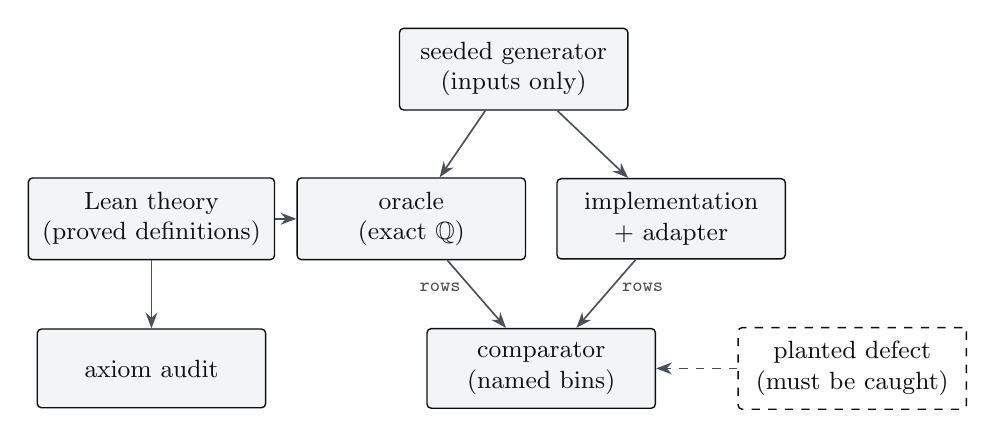
\begin{tikzpicture}[
  box/.style={draw=Ink, line width=0.5pt, fill=Surface, text=Ink, rounded corners=1.5pt,
    align=center, font=\small, inner sep=5pt, minimum height=10mm, minimum width=29mm},
  arr/.style={-{Stealth[length=2mm]}, line width=0.6pt, draw=InkMuted},
  lab/.style={font=\ttfamily\scriptsize, text=InkMuted}]
\node[box] (gen) at (4.6,1.9) {seeded generator\\(inputs only)};
\node[box] (theory) at (0,0) {Lean theory\\(proved definitions)};
\node[box] (oracle) at (3.3,0) {oracle\\(exact $\mathbb{Q}$)};
\node[box] (impl) at (6.6,0) {implementation\\+ adapter};
\node[box] (cmp) at (4.95,-1.9) {comparator\\(named bins)};
\node[box] (audit) at (0,-1.9) {axiom audit};
\node[box, dashed, fill=Background] (planted) at (8.9,-1.9) {planted defect\\(must be caught)};
\draw[arr] (gen) -- (oracle);
\draw[arr] (gen) -- (impl);
\draw[arr] (theory) -- (oracle);
\draw[arr] (theory) -- (audit);
\draw[arr] (oracle) -- node[left, lab, pos=0.4] {rows} (cmp);
\draw[arr] (impl) -- node[right, lab, pos=0.4] {rows} (cmp);
\draw[arr, dashed] (planted) -- (cmp);
\end{tikzpicture}
\caption{The measurement procedure. The generator never computes expected results;
those come only from the oracle.}
\label{fig:harness}
\end{figure}

The procedure follows \texttt{ledger-semantics} (\cref{fig:harness}). A seeded
generator writes case files containing inputs only. It favors the inputs where
implementations are known to have conventions: tied logits, words that are
themselves tokens, and merge tables with several splits of one string. A small
adapter per implementation runs the same cases and prints the oracle's row format.
The comparator places every case in exactly one named bin (agree, diverge, skipped
by either side, or missing), so nothing is dropped silently. Token rows are compared
as strings. Sampler rows require that a zero be matched by a zero and that nonzero
probabilities agree within $10^{-6}$, since llama.cpp stores logits in
\texttt{float32}. Each comparator is observed to fail: a planted defect, an adapter
that glues two tokens or one that inverts temperature, must be detected or the run
fails.

\paragraph{Tie divergences.} An implementation that keeps exactly $k$ tokens breaks
ties in its own order, which need not be the oracle's order by index. Every filter
treats tied tokens alike except for that choice, and tied tokens stay tied through
temperature and renormalization. Such an implementation must therefore agree with
the positional semantics up to a permutation of tied tokens. The harness checks
exactly this: the multiset of (logit, probability) pairs over the kept tokens must
equal that of the oracle's \texttt{q} rows. A divergence that fails this check is
reported as unexplained.

\begin{table}[t]
\centering\small
\caption{Measurements (\texttt{harness/run.sh 600}: four seeds of 600 cases each per
corpus). Lean 4.34.1, Mathlib v4.34.1, \texttt{tokenizers} 0.23.3, \texttt{tiktoken}
0.14.0, llama.cpp commit \texttt{a9d27ac} (2026-10-11).}
\label{tab:results}
\begin{tabularx}{\linewidth}{@{}>{\raggedright\arraybackslash}p{4.6cm}>{\raggedright\arraybackslash}X>{\raggedright\arraybackslash}X@{}}
\toprule
\qpth{Implementation} & \qpth{Compared against} & \qpth{Result}\\
\midrule
HF \texttt{tokenizers}, BPE, defaults & rule-rank BPE (\lean{bpe}) & 13{,}779 / 13{,}779 words identical\\
HF \texttt{tokenizers}, \lean{ignore_merges} & lookup, then rule-rank BPE & 13{,}779 / 13{,}779 identical\\
\texttt{tiktoken} & lookup, then concatenation-rank BPE & 13{,}779 / 13{,}779 identical\\
llama.cpp \lean{top_k}, \lean{top_p}, \lean{min_p}, \texttt{temp}, no ties & tie-keeping filters & 1{,}216 / 1{,}216 chains, $|\Delta p|\le5.1\times10^{-8}$\\
llama.cpp, with ties & tie-keeping, else positional & 939 + 245 / 1{,}184 chains; 0 unexplained\\
Planted defects (tokenizer, sampler) & --- & both detected\\
\bottomrule
\end{tabularx}
\end{table}

\Cref{tab:results} summarizes the results. Two findings came out of the
comparisons. First, \texttt{tiktoken} initially disagreed with the oracle's
concatenation-rank BPE on words that are themselves vocabulary tokens. The
disagreement was a convention, whole-word lookup. Following the
\texttt{ledger-semantics} rule that a divergence is either a defect in the
implementation or a convention the semantics has not yet recorded, we recorded it
as \lean{lookupFirst}, with its own theorems, after which agreement is exact.
Second, on the same random merge tables the two tokenizer libraries disagree with
each other on 439 of 13{,}779 words (3.2\%), and on 279 when Hugging Face uses
\lean{ignore_merges}. The oracle reproduces each library exactly, so every one of
these disagreements is predicted. \Cref{thm:bpeconv} states the condition under which
they cannot occur.

For sampling, llama.cpp agrees with the tie-keeping semantics on every tie-free
chain. On chains with ties, 245 of 1{,}184 diverge, and every one agrees with the
positional semantics up to a permutation of tied tokens. Some of these divergences
cascade: a tie cut by top-$k$ changes the renormalized masses that a later top-$p$
sees. A check that compared kept sets only after the fact would misclassify such
cases. Replaying the convention exactly classifies all of them.

% ===========================================================================
\section{Related work}

\paragraph{Formal methods for machine learning.} Most verification work on neural
networks proves properties of trained models, for example with SMT-based
methods~\cite{katz2017reluplex}. We verify the model-independent algorithms around
the model instead, and connect them to implementations through an oracle. The
denotational method follows Elliott~\cite{elliott2009denotational}. The use of a
proved semantics as a test oracle, the procedure of planted defects, and the
discipline of named skip bins follow \texttt{ledger-semantics}~\cite{ledgersemantics}.
Our category of finite stochastic maps is a special case of Fritz's Markov
categories~\cite{fritz2020markov}.

\paragraph{Tokenization.} Zouhar et al.\ give a formal analysis of BPE as an
optimization problem~\cite{zouhar2023bpe}. Gastaldi et al.\ treat tokenizers as
stochastic maps and study consistency of estimators~\cite{gastaldi2024foundations}.
Vieira et al.\ show how to turn token-level models into character-level
ones~\cite{vieira2024tokens}, which requires exactly the enumeration of
tokenizations we verify. Our no-compression theorem and the agreement criterion
between BPE conventions complement this work at the level of exact identities.

\paragraph{Decoding.} Top-$k$~\cite{fan2018hierarchical}, nucleus~\cite{holtzman2020curious}
and min-$p$~\cite{nguyen2025minp} sampling are usually specified by an algorithm over
sorted arrays, which leaves ties unspecified. \Cref{thm:topk} shows that this gap
cannot be closed by any symmetric rule. Speculative
sampling~\cite{leviathan2023speculative,chen2023speculative} is known to be lossless,
and its acceptance rate is the maximal-coupling bound~\cite{lindvall1992coupling}. Du et
al.\ characterize tightness measure-theoretically~\cite{du2023tight}. We give a
finite-depth statement and an explicit non-tight model.

\paragraph{Attention and inference systems.} Online softmax~\cite{milakov2018online}
underlies FlashAttention~\cite{dao2022flashattention} and its successors, and
KV caching is standard in serving systems~\cite{pope2023scaling,kwon2023vllm}. Our
contribution is the algebraic packaging, a commutative monoid with a free-monoid
homomorphism, and machine-checked proofs over arbitrary exponential characters.
Permutation equivariance of attention without positional encodings is
known~\cite{yun2020universal}.

\paragraph{Masked diffusion.} The time-independence of the optimal denoiser was
observed by Ou et al.~\cite{ou2025absorbing}, in the setting of
D3PM~\cite{austin2021d3pm}, MDLM~\cite{sahoo2024mdlm} and related
models~\cite{shi2024masked,nie2025llada}. We machine-check it, together with the
any-order chain rule and the inexactness of parallel unmasking.

% ===========================================================================
\section{Limitations}

Analysis on the reals enters only through exponential characters, and there is no
measure theory, so sampling and tightness are stated through finite quantities. The
oracle's temperature is restricted to $1/n$, which keeps softmax rational. The
theorems hold for every temperature, but the oracle cannot evaluate an irrational
softmax. Speculative decoding is proved for one drafted token. The sequence version
follows by induction and is not yet formalized. Nothing is proved about
floating-point arithmetic: implementations are compared with exact values within a
stated tolerance. A decision that lies exactly on a floating-point boundary could in
principle diverge, and none occurred in our runs. The diffusion theory covers
absorbing diffusion, not Gaussian diffusion. The chat protocol models tool calling in
its common request-and-result form, not any vendor's specification. The measurements
cover tokenizers and samplers; attention kernels, speculative decoders, chat
renderers and diffusion samplers are evaluated by the oracle but not yet compared
against implementations.

% ===========================================================================
\section{Conclusion}

The inference side of LLMs is small enough to be given a precise meaning and large
enough that its implementations disagree. A machine-checked semantics separates
what is meaning from what is convention. It proves which reorderings, cachings and
tilings are harmless, and it shows that some properties folklore expects, such as
symmetric exact top-$k$, compositional compressing tokenizers and unambiguous plain-text
templates, cannot exist. Connected to an exact oracle, the same definitions become
a test instrument. Every divergence it surfaces is either a defect in an
implementation or a convention that belongs in the semantics.

\paragraph{Availability.} The Lean development, oracle, harness, and recorded
measurement log accompany this paper.

\paragraph{Acknowledgments.} The structure of this work follows
\texttt{ledger-semantics} by John Wiegley. The formalization and harness were
developed with the assistance of an AI system (Claude, Anthropic).

% ===========================================================================
\begin{thebibliography}{99}\small

\bibitem{austin2021d3pm}
J.~Austin, D.~D. Johnson, J.~Ho, D.~Tarlow, and R.~van~den Berg.
\newblock Structured denoising diffusion models in discrete state-spaces.
\newblock In \emph{NeurIPS}, 2021.

\bibitem{chen2023speculative}
C.~Chen, S.~Borgeaud, G.~Irving, J.-B. Lespiau, L.~Sifre, and J.~Jumper.
\newblock Accelerating large language model decoding with speculative sampling.
\newblock arXiv:2302.01318, 2023.

\bibitem{dao2022flashattention}
T.~Dao, D.~Y. Fu, S.~Ermon, A.~Rudra, and C.~R{\'e}.
\newblock {FlashAttention}: Fast and memory-efficient exact attention with {IO}-awareness.
\newblock In \emph{NeurIPS}, 2022.

\bibitem{demoura2021lean4}
L.~de~Moura and S.~Ullrich.
\newblock The {Lean} 4 theorem prover and programming language.
\newblock In \emph{CADE-28}, 2021.

\bibitem{du2023tight}
L.~Du, L.~Torroba~Hennigen, T.~Pimentel, C.~Meister, J.~Eisner, and R.~Cotterell.
\newblock A measure-theoretic characterization of tight language models.
\newblock In \emph{ACL}, 2023.

\bibitem{elliott2009denotational}
C.~Elliott.
\newblock Denotational design with type class morphisms.
\newblock Technical Report 2009-01, LambdaPix, 2009.

\bibitem{fan2018hierarchical}
A.~Fan, M.~Lewis, and Y.~Dauphin.
\newblock Hierarchical neural story generation.
\newblock In \emph{ACL}, 2018.

\bibitem{fritz2020markov}
T.~Fritz.
\newblock A synthetic approach to {Markov} kernels, conditional independence and theorems on sufficient statistics.
\newblock \emph{Advances in Mathematics}, 370, 2020.

\bibitem{gastaldi2024foundations}
J.~L. Gastaldi, J.~Terilla, L.~Malagutti, B.~DuSell, T.~Vieira, and R.~Cotterell.
\newblock The foundations of tokenization: Statistical and computational concerns.
\newblock arXiv:2407.11606, 2024.

\bibitem{greshake2023injection}
K.~Greshake, S.~Abdelnabi, S.~Mishra, C.~Endres, T.~Holz, and M.~Fritz.
\newblock Not what you've signed up for: Compromising real-world {LLM}-integrated applications with indirect prompt injection.
\newblock In \emph{AISec}, 2023.

\bibitem{holtzman2020curious}
A.~Holtzman, J.~Buys, L.~Du, M.~Forbes, and Y.~Choi.
\newblock The curious case of neural text degeneration.
\newblock In \emph{ICLR}, 2020.

\bibitem{katz2017reluplex}
G.~Katz, C.~Barrett, D.~L. Dill, K.~Julian, and M.~J. Kochenderfer.
\newblock Reluplex: An efficient {SMT} solver for verifying deep neural networks.
\newblock In \emph{CAV}, 2017.

\bibitem{kwon2023vllm}
W.~Kwon, Z.~Li, S.~Zhuang, Y.~Sheng, L.~Zheng, C.~H. Yu, J.~E. Gonzalez, H.~Zhang, and I.~Stoica.
\newblock Efficient memory management for large language model serving with {PagedAttention}.
\newblock In \emph{SOSP}, 2023.

\bibitem{ledgersemantics}
J.~Wiegley.
\newblock ledger-semantics: Mathematical semantics of {Ledger}, the double-entry accounting tool.
\newblock \url{https://github.com/ledger/ledger-semantics}, 2026.

\bibitem{leviathan2023speculative}
Y.~Leviathan, M.~Kalman, and Y.~Matias.
\newblock Fast inference from transformers via speculative decoding.
\newblock In \emph{ICML}, 2023.

\bibitem{lindvall1992coupling}
T.~Lindvall.
\newblock \emph{Lectures on the Coupling Method}.
\newblock Wiley, 1992.

\bibitem{liu2023ring}
H.~Liu, M.~Zaharia, and P.~Abbeel.
\newblock Ring attention with blockwise transformers for near-infinite context.
\newblock arXiv:2310.01889, 2023.

\bibitem{mathlib2020}
The mathlib Community.
\newblock The {Lean} mathematical library.
\newblock In \emph{CPP}, 2020.

\bibitem{milakov2018online}
M.~Milakov and N.~Gimelshein.
\newblock Online normalizer calculation for softmax.
\newblock arXiv:1805.02867, 2018.

\bibitem{nguyen2025minp}
M.~N. Nguyen, A.~Baker, C.~Neo, A.~Roush, A.~Kirsch, and R.~Shwartz-Ziv.
\newblock Turning up the heat: Min-p sampling for creative and coherent {LLM} outputs.
\newblock In \emph{ICLR}, 2025.

\bibitem{nie2025llada}
S.~Nie, F.~Zhu, Z.~You, X.~Zhang, J.~Ou, J.~Hu, J.~Zhou, Y.~Lin, J.-R. Wen, and C.~Li.
\newblock Large language diffusion models.
\newblock arXiv:2502.09992, 2025.

\bibitem{ou2025absorbing}
J.~Ou, S.~Nie, K.~Xue, F.~Zhu, J.~Sun, Z.~Li, and C.~Li.
\newblock Your absorbing discrete diffusion secretly models the conditional distributions of clean data.
\newblock In \emph{ICLR}, 2025.

\bibitem{pope2023scaling}
R.~Pope, S.~Douglas, A.~Chowdhery, J.~Devlin, J.~Bradbury, J.~Heek, K.~Xiao, S.~Agrawal, and J.~Dean.
\newblock Efficiently scaling transformer inference.
\newblock In \emph{MLSys}, 2023.

\bibitem{rabe2021selfattention}
M.~N. Rabe and C.~Staats.
\newblock Self-attention does not need {$O(n^2)$} memory.
\newblock arXiv:2112.05682, 2021.

\bibitem{radford2019gpt2}
A.~Radford, J.~Wu, R.~Child, D.~Luan, D.~Amodei, and I.~Sutskever.
\newblock Language models are unsupervised multitask learners.
\newblock OpenAI technical report, 2019.

\bibitem{sahoo2024mdlm}
S.~S. Sahoo, M.~Arriola, Y.~Schiff, A.~Gokaslan, E.~Marroquin, J.~T. Chiu, A.~Rush, and V.~Kuleshov.
\newblock Simple and effective masked diffusion language models.
\newblock In \emph{NeurIPS}, 2024.

\bibitem{sennrich2016bpe}
R.~Sennrich, B.~Haddow, and A.~Birch.
\newblock Neural machine translation of rare words with subword units.
\newblock In \emph{ACL}, 2016.

\bibitem{shi2024masked}
J.~Shi, K.~Han, Z.~Wang, A.~Doucet, and M.~K. Titsias.
\newblock Simplified and generalized masked diffusion for discrete data.
\newblock In \emph{NeurIPS}, 2024.

\bibitem{vieira2024tokens}
T.~Vieira, B.~LeBrun, M.~Giulianelli, J.~L. Gastaldi, B.~DuSell, J.~Terilla, T.~J. O'Donnell, and R.~Cotterell.
\newblock From language models over tokens to language models over characters.
\newblock arXiv:2412.03719, 2024.

\bibitem{wolf2020transformers}
T.~Wolf et~al.
\newblock Transformers: State-of-the-art natural language processing.
\newblock In \emph{EMNLP: System Demonstrations}, 2020.

\bibitem{xiao2024sinks}
G.~Xiao, Y.~Tian, B.~Chen, S.~Han, and M.~Lewis.
\newblock Efficient streaming language models with attention sinks.
\newblock In \emph{ICLR}, 2024.

\bibitem{yun2020universal}
C.~Yun, S.~Bhojanapalli, A.~S. Rawat, S.~J. Reddi, and S.~Kumar.
\newblock Are transformers universal approximators of sequence-to-sequence functions?
\newblock In \emph{ICLR}, 2020.

\bibitem{zouhar2023bpe}
V.~Zouhar, C.~Meister, J.~L. Gastaldi, L.~Du, T.~Vieira, M.~Sachan, and R.~Cotterell.
\newblock A formal perspective on byte-pair encoding.
\newblock In \emph{Findings of ACL}, 2023.

\end{thebibliography}

\end{document}
"

\usepackage[a4paper,textwidth=15.4cm,textheight=23.6cm,top=3.0cm,headsep=0.9cm,footskip=1.2cm]{geometry}
\usepackage{amsmath,amssymb,amsthm,mathtools}
\usepackage{fontspec}
\usepackage{booktabs,tabularx,array}
\usepackage[protrusion=true,expansion=false]{microtype}
\usepackage[table]{xcolor}
\usepackage{graphicx}
\usepackage{fvextra}
\usepackage{enumitem}
\usepackage{caption}
\usepackage{titlesec}
\usepackage{fancyhdr}
\usepackage[most]{tcolorbox}
\usepackage{tikz}
\usetikzlibrary{arrows.meta}
\usepackage{hyperref}
\usepackage[nameinlink,capitalise]{cleveref}

% ---------------------------------------------------------------------------
%  Colour tokens
% ---------------------------------------------------------------------------
% Neutral foundation. Ink and Background invert between the two editions.
\ifqptdark
  \definecolor{Background}{HTML}{0B0C0E}
  \definecolor{Surface}{HTML}{16181B}
  \definecolor{Border}{HTML}{2B2E33}
  \definecolor{Ink}{HTML}{EDEEF0}
  \definecolor{InkMuted}{HTML}{A9AEB6}
  \definecolor{InkFaint}{HTML}{5A5F67}   % decoration only, never meaningful text
\else
  \definecolor{Background}{HTML}{FFFFFF}
  \definecolor{Surface}{HTML}{F3F4F5}
  \definecolor{Border}{HTML}{DADDE1}
  \definecolor{Ink}{HTML}{0E0F11}
  \definecolor{InkMuted}{HTML}{4B4F57}
  \definecolor{InkFaint}{HTML}{A3A7AE}   % decoration only, never meaningful text
\fi
% Paradigm colours: fixed in both editions, semantic only.
\definecolor{Quantum}{HTML}{5BAD1E}
\definecolor{Photonic}{HTML}{F0AB00}
\definecolor{Thermodynamic}{HTML}{E8690A}
\definecolor{Ternary}{HTML}{8A8A8A}
\definecolor{Bio}{HTML}{1AAB7C}

\ifqptdark\pagecolor{Background}\fi

% ---------------------------------------------------------------------------
%  Typography
% ---------------------------------------------------------------------------
\setmainfont{Inter}[
  Path=fonts/, Extension=.otf, Scale=0.94,
  UprightFont=*-Regular, ItalicFont=*-Italic,
  BoldFont=*-SemiBold, BoldItalicFont=*-SemiBoldItalic]
\setmonofont{IBMPlexMono}[
  Path=fonts/, Extension=.ttf, Scale=MatchLowercase,
  UprightFont=*-Regular, ItalicFont=*-Italic, BoldFont=*-SemiBold]
\newfontfamily\qptdisplay{SpaceGrotesk}[
  Path=fonts/, Extension=.otf, UprightFont=*-Medium, BoldFont=*-Bold]
\newfontfamily\qptdisplaylight{SpaceGrotesk}[
  Path=fonts/, Extension=.otf, UprightFont=*-Regular]
\newfontfamily\qptlabelfont{IBMPlexMono}[
  Path=fonts/, Extension=.ttf, Scale=MatchLowercase, UprightFont=*-Medium,
  LetterSpace=6]
\setsansfont{Inter}[
  Path=fonts/, Extension=.otf, Scale=0.94,
  UprightFont=*-Regular, ItalicFont=*-Italic,
  BoldFont=*-SemiBold, BoldItalicFont=*-SemiBoldItalic]
\linespread{1.16}
\setlength{\emergencystretch}{2.5em}
\AtBeginDocument{\raggedright\setlength{\parindent}{0pt}}
\setlength{\parindent}{0pt}
\setlength{\parskip}{0.55em}

% A label: IBM Plex Mono, upper case, tracked.
\newcommand{\qptlabel}[1]{{\qptlabelfont\footnotesize\MakeUppercase{#1}}}
% Technical names (Lean declarations, files) in IBM Plex Mono.
\newcommand{\lean}[1]{\texttt{\detokenize{#1}}}
\newcommand{\leanref}[1]{\par\smallskip\noindent
  {\ttfamily\footnotesize\upshape\raggedright\color{InkMuted}LEAN\enspace #1\par}}

% Ink is the normal colour everywhere, including floats, heads and footnotes.
\makeatletter
\AtBeginDocument{\color{Ink}\global\let\default@color\current@color}
\makeatother

% ---------------------------------------------------------------------------
%  Mathematical notation
% ---------------------------------------------------------------------------
\newcommand{\K}{\Bbbk}
\newcommand{\Dist}{\mathrm{Dist}}
\newcommand{\restr}[2]{#1|_{#2}}
\newcommand{\topk}{\mathrm{TopK}}
\newcommand{\topp}{\mathrm{TopP}}
\newcommand{\minp}{\mathrm{MinP}}
\newcommand{\sharpen}{\mathrm{sharpen}}
\newcommand{\abv}{\mathrm{above}}
\newcommand{\tv}{\mathrm{tv}}
\newcommand{\dec}{\mathrm{dec}}
\newcommand{\enc}{\mathrm{enc}}
\newcommand{\softmax}{\mathrm{softmax}}
\newcommand{\attend}{\mathrm{attend}}
\newcommand{\Iv}[1]{[\![#1]\!]}
\newcommand{\Mask}{\bot}

% ---------------------------------------------------------------------------
%  Headings: section numbers as labels, titles in Space Grotesk
% ---------------------------------------------------------------------------
\makeatletter
\newcommand{\qptsecnum}[1]{{\qptlabelfont\small\color{InkMuted}\two@digits{#1}}}
\makeatother
\titleformat{\section}
  {\qptdisplay\fontsize{14.5}{18}\selectfont\color{Ink}}
  {\qptsecnum{\value{section}}}{0.9em}{}
\titleformat{name=\section,numberless}
  {\qptdisplay\fontsize{14.5}{18}\selectfont\color{Ink}}{}{0pt}{}
\titlespacing*{\section}{0pt}{1.9em}{0.7em}
\titleformat{\paragraph}[runin]
  {\qptdisplay\normalsize\color{Ink}}{}{0pt}{}
\titlespacing*{\paragraph}{0pt}{0.9em}{0.6em}

% ---------------------------------------------------------------------------
%  Statements
% ---------------------------------------------------------------------------
\newtheoremstyle{qpt}
  {0.9em}{0.9em}
  {\normalfont}{}
  {\qptlabelfont\footnotesize}{}
  {\newline}
  {\MakeUppercase{\thmname{#1}\thmnumber{~#2}}%
   \thmnote{\enspace{\qptdisplay\normalsize\color{Ink}#3}}}
\theoremstyle{qpt}
\newtheorem{theorem}{Theorem}
\newtheorem{proposition}[theorem]{Proposition}
\newtheorem{corollary}[theorem]{Corollary}
\newtheorem{lemma}[theorem]{Lemma}
\newtheorem{definition}[theorem]{Definition}
\newtheorem{remark}[theorem]{Remark}

% Proofs: a tracked label and a neutral end mark.
\makeatletter
\renewcommand{\qedsymbol}{{\color{InkMuted}\rule{0.5em}{0.5em}}}
\renewenvironment{proof}[1][Proof]{\par\pushQED{\qed}\normalfont\topsep0.5em\relax
  \trivlist\item[\hskip\labelsep\qptlabel{#1}\hspace{0.6em}]\ignorespaces}
  {\popQED\endtrivlist\@endpefalse}
\makeatother

% ---------------------------------------------------------------------------
%  Code: IBM Plex Mono on a neutral surface, with a hairline on the left
% ---------------------------------------------------------------------------
\tcbset{colupper=Ink, collower=Ink}
\tcbset{qptcode/.style={enhanced, colback=Surface, colframe=Surface,
  boxrule=0pt, arc=0pt, left=9pt, right=8pt, top=5pt, bottom=5pt,
  borderline west={1.2pt}{0pt}{InkFaint}, before skip=0.7em, after skip=0.7em}}
\newenvironment{leancode}
  {\VerbatimEnvironment\begin{tcolorbox}[qptcode]%
   \begin{Verbatim}[fontsize=\small,commandchars=\\\{\},
     codes={\catcode`\$=3\catcode`\^=7},formatcom=\color{Ink}]}
  {\end{Verbatim}\end{tcolorbox}}
\newenvironment{casecode}
  {\VerbatimEnvironment\begin{tcolorbox}[qptcode,before skip=0pt,after skip=0pt]%
   \begin{Verbatim}[fontsize=\footnotesize,formatcom=\color{Ink}]}
  {\end{Verbatim}\end{tcolorbox}}

% ---------------------------------------------------------------------------
%  Floats, tables, captions
% ---------------------------------------------------------------------------
\DeclareCaptionLabelFormat{qpt}{\qptlabel{#1~#2}}
\DeclareCaptionLabelSeparator{qptsep}{\quad}
\captionsetup{labelformat=qpt, labelsep=qptsep, font={small,color=Ink},
  justification=raggedright, singlelinecheck=false, skip=6pt}
\newcommand{\qpth}[1]{\qptlabel{#1}}
\arrayrulecolor{Ink}
\setlength{\heavyrulewidth}{0.7pt}
\setlength{\lightrulewidth}{0.35pt}
\renewcommand{\arraystretch}{1.22}

% ---------------------------------------------------------------------------
%  Running heads
% ---------------------------------------------------------------------------
\pagestyle{fancy}
\fancyhf{}
\fancyhead[L]{{\color{Ink}\qptlabel{Machine-checked semantics of LLM inference}}}
\fancyhead[R]{{\color{Ink}\qptlabel{D. Arango Sohm}}}
\fancyfoot[R]{{\ttfamily\small\color{InkMuted}\thepage}}
\renewcommand{\headrule}{{\color{Border}\hrule height 0.4pt}\vspace{-0.4pt}}
\renewcommand{\headrulewidth}{0.4pt}
\fancypagestyle{qptfirst}{\fancyhf{}%
  \fancyfoot[R]{{\ttfamily\small\color{InkMuted}\thepage}}%
  \renewcommand{\headrulewidth}{0pt}\renewcommand{\headrule}{}}

% ---------------------------------------------------------------------------
%  Links and references: neutral, never accent-coloured text
% ---------------------------------------------------------------------------
\hypersetup{colorlinks=true, linkcolor=Ink, citecolor=Ink, urlcolor=Ink,
  pdftitle={A Machine-Checked Semantics of LLM Inference},
  pdfauthor={Daniel Arango Sohm},
  pdfsubject={Formal semantics of large language model inference in Lean 4},
  pdfkeywords={Lean 4, Mathlib, formal verification, LLM inference, sampling,
    tokenization, attention, speculative decoding, diffusion language models}}
\makeatletter
\renewcommand{\@biblabel}[1]{{\ttfamily\color{InkMuted}[#1]}}
\renewcommand{\@cite}[2]{{\ttfamily[#1\if@tempswa, #2\fi]}}
\makeatother
\renewcommand{\refname}{References}

\setlist{itemsep=2pt, topsep=4pt}
\setlist[itemize]{label={\color{InkMuted}\textbullet}}

\begin{document}
\thispagestyle{qptfirst}

% ----------------------------------------------------------------- masthead
\noindent
\begin{minipage}[c]{0.5\linewidth}
  \includegraphics[height=1.9cm]{qpt-logo.png}
\end{minipage}%
\begin{minipage}[c]{0.5\linewidth}\raggedleft
  \qptlabel{Preprint}\\[2pt]
  \qptlabel{October 2026}
\end{minipage}

\vspace{1.6em}
{\color{Border}\rule{\linewidth}{0.4pt}}
\vspace{1.1em}

{\qptdisplay\fontsize{25}{29.5}\selectfont\color{Ink}
A Machine-Checked Semantics\\ of LLM Inference\par}
\vspace{0.55em}
{\qptdisplaylight\fontsize{13}{17}\selectfont\color{InkMuted}
Sampling, Attention, Tokenization, Chat, Decoding,\\ and Diffusion in Lean~4\par}

\vspace{1.5em}
{\large\bfseries Daniel Arango Sohm}\par
\vspace{0.15em}
{\color{InkMuted}Universidad EAFIT, Medellín, Colombia\\
Former member of the QPT team}\par

\vspace{1.4em}
% ----------------------------------------------------------------- abstract
\begin{tcolorbox}[enhanced, colback=Surface, colframe=Surface, colupper=Ink, boxrule=0pt,
  arc=0pt, left=12pt, right=12pt, top=9pt, bottom=10pt]
\qptlabel{Abstract}\par\vspace{0.35em}
{\small
The inference side of a large language model is a stack of small algorithms:
tokenizers, attention kernels, key--value caches, sampling filters, speculative
decoders, chat templates, and diffusion samplers. Each has several independent
implementations, and those implementations are usually tested against one another
rather than against a definition. We give these components a single mathematical
semantics, formalized in Lean~4 against Mathlib. The development comprises about
4{,}600 lines and 270 named theorems, and every declaration depends only on Lean's
three standard axioms. It proves the exact algebra of sampling filters, the
losslessness and optimality of speculative sampling, and the correctness of
key--value caching and of FlashAttention-style online softmax as a commutative
monoid. It proves that byte-pair encoding is lossless under every merge priority,
together with a decidable criterion for when the Hugging Face and \texttt{tiktoken}
conventions agree, a protocol checker for tool calls, and the time-independence of
the masked-diffusion denoiser. It also proves six negative results. No sampling
rule that treats tokens symmetrically can always keep exactly $k$ tokens. No
tokenizer that compresses can respect concatenation. Every chat template that writes
its role markers in the content alphabet is ambiguous. No transformer without
positional information can copy a fixed position. An autoregressive model need not
define a distribution over strings. Parallel unmasking in diffusion is inexact.
From the same definitions we build an executable oracle that evaluates test cases in
exact rational arithmetic, and a harness that measures implementations against it.
On 2{,}400 random merge tables, Hugging Face \texttt{tokenizers} and
\texttt{tiktoken} each agree with the oracle on all 13{,}779 test words, while
disagreeing with each other on 3.2\% of them. On 2{,}400 random sampler chains,
every divergence of llama.cpp from the tie-keeping semantics is accounted for
exactly by the positional semantics that the impossibility theorem forces.
\par}
\end{tcolorbox}

\vspace{0.3em}
\noindent\qptlabel{Keywords}\enspace{\small Lean~4 · Mathlib · formal verification ·
LLM inference · sampling · tokenization · attention · speculative decoding ·
diffusion language models}

\vspace{0.4em}
{\color{Border}\rule{\linewidth}{0.4pt}}

% ===========================================================================
\section{Introduction}

A deployed language model is a function from parameters and a context to a
distribution over tokens. Turning that distribution into text requires more
machinery. A tokenizer maps strings to token sequences. Attention kernels compute
the model's reads over a cached context. A chain of sampling filters reshapes the
next-token distribution. A speculative decoder may verify drafted tokens, a chat
template linearizes a conversation, and a diffusion sampler may unmask several
positions at once. Each of these components exists in many implementations, such as
Hugging Face \texttt{transformers} and \texttt{tokenizers}~\cite{wolf2020transformers},
\texttt{tiktoken}, vLLM~\cite{kwon2023vllm}, and llama.cpp. Their tests mostly
compare one implementation with another, or with remembered behavior.

This paper follows a different discipline, \emph{denotational design}~\cite{elliott2009denotational}.
One first says precisely what a thing means, then requires every operation to
preserve that meaning, and lets the implementation be whatever the equations force
it to be. The approach is that of \texttt{ledger-semantics}~\cite{ledgersemantics},
which formalizes double-entry accounting in Lean and uses the result as a test oracle
for the C++ Ledger program. We apply it to LLM inference. A sampling filter means
conditioning a distribution on a set. A KV-cached decoder means causal attention over
the whole prefix. A FlashAttention kernel means a softmax-weighted average. A chat
template means an injective encoding of a transcript. The theorems state when an
implementation preserves that meaning, and several of them state that no
implementation can.

\paragraph{Contributions.}
\begin{itemize}[leftmargin=*,itemsep=2pt]
\item A Lean~4 formalization against Mathlib~\cite{mathlib2020,demoura2021lean4}
  of sampling, speculative decoding, softmax and attention, tokenization, chat
  transcripts, autoregressive decoding, and masked diffusion
  (\cref{sec:foundations,sec:sampling,sec:spec,sec:attention,sec:tokenization,sec:chat,sec:decoding,sec:diffusion}).
  All definitions are stated over an arbitrary linearly ordered field, so one proof
  covers the real numbers of the literature and the exact rationals of the oracle.
\item Positive results in a common framework. They include the algebra of
  sampling filters, the optimality of speculative sampling, an online-softmax
  commutative monoid, a generic correctness theorem for BPE with a decidable
  agreement criterion between the two conventions in use, a protocol checker for
  tool calls, and the any-order chain rule for masked diffusion.
\item Six negative results that explain design constraints visible across
  implementations (\cref{sec:negative}).
\item An executable oracle that evaluates case files under the proved
  definitions in exact arithmetic, and a measurement of Hugging Face
  \texttt{tokenizers}, \texttt{tiktoken}, and llama.cpp against it (\cref{sec:oracle,sec:measure}).
\end{itemize}

Several of the positive results are known: losslessness of speculative
sampling~\cite{leviathan2023speculative,chen2023speculative}, correctness of online
softmax~\cite{milakov2018online,dao2022flashattention}, time-independence of the
absorbing-diffusion posterior~\cite{ou2025absorbing}, and the role of permutation
equivariance~\cite{yun2020universal}. Our contribution for these is a machine-checked
statement in one framework, connected to an oracle. To our knowledge the
following are not stated elsewhere in the form given here: the impossibility of
symmetric exact top-$k$ and nucleus selection, the no-compression theorem for
homomorphic tokenizers, the ambiguity of every in-band chat template, and the
decidable agreement criterion between merge-rule and concatenation-rank BPE.

% ===========================================================================
\section{Method and trust base}\label{sec:method}

The development is a Lean~4 library (Lean 4.34.1, Mathlib v4.34.1) of eleven
theory modules and two executable modules (\cref{tab:modules}). It is built with
warnings promoted to errors, so an unproved theorem (\lean{sorry}) fails the build.
A separate audit program walks every declaration in the library, 853 in all, and
fails unless each depends only on propositional extensionality, the axiom of choice,
and quotient soundness. The audit has been observed to fail: a planted proof by
\lean{native_decide}, which introduces an auxiliary axiom trusting compiled code, is
rejected. The warnings-as-errors build alone does not catch it. Concrete
counterexamples are therefore proved by \lean{decide}, whose certificate the kernel
checks by evaluation.

\begin{table}[t]
\centering\small
\caption{Modules of the development. Lines and named theorems and lemmas per module.}
\label{tab:modules}
\begin{tabularx}{\linewidth}{@{}l>{\raggedright\arraybackslash}X>{\ttfamily}r>{\ttfamily}r@{}}
\toprule
\qpth{Module} & \qpth{Content} & \qpth{Lines} & \qpth{Thms} \\
\midrule
\lean{Dist} & finite distributions, conditioning, total variation, $\mathsf{FinStoch}$ & 383 & 34\\
\lean{Sampling} & top-$k$, top-$p$, min-$p$, temperature, ties, inverse CDF & 732 & 46\\
\lean{Counterexamples} & kernel-checked failures of sampler laws & 52 & 4\\
\lean{Speculative} & speculative sampling, couplings & 194 & 17\\
\lean{Softmax} & exponential characters, masking, temperature & 220 & 23\\
\lean{Attention} & equivariance, causality, KV cache, online softmax & 573 & 38\\
\lean{Real} & $\exp$ as a character; textbook restatements & 51 & 4\\
\lean{Tokenization} & free-monoid decoding, BPE conventions, enumeration & 860 & 49\\
\lean{Chat} & tool-call protocol, rendering & 440 & 21\\
\lean{Decoding} & mass conservation, tightness, greedy decoding & 245 & 15\\
\lean{Diffusion} & masked diffusion, posterior, chain rule & 379 & 18\\
\lean{Oracle}, \lean{Driver} & case parsing and exact evaluation & 465 & 1\\
\midrule
Total & & 4{,}594 & 270\\
\bottomrule
\end{tabularx}
\end{table}

\paragraph{Numbers.} Every probability lives in an arbitrary field $\K$ with a
compatible linear order (\lean{[Field K] [LinearOrder K] [IsStrictOrderedRing K]}).
The oracle instantiates $\K=\mathbb{Q}$, so its arithmetic is exact. The analytic
statements instantiate $\K=\mathbb{R}$. No measure theory is used. Sampling is made
precise through interval statements (\cref{thm:invcdf}), and tightness through
masses at finite depth (\cref{sec:decoding}).

% ===========================================================================
\section{Foundations}\label{sec:foundations}

\begin{definition}[Finite distribution]
For a finite type $\alpha$, $\Dist_\K(\alpha)$ is the type of functions
$p:\alpha\to\K$ with $p(a)\ge 0$ for all $a$ and $\sum_a p(a)=1$.
\leanref{\lean{Dist}}
\end{definition}

\begin{leancode}
structure Dist ($\K$ : Type u) [Field $\K$] [LinearOrder $\K$] [IsStrictOrderedRing $\K$]
    ($\alpha$ : Type v) [Fintype $\alpha$] where
  prob : $\alpha$ $\to$ $\K$
  nonneg : $\forall$ a, 0 $\le$ prob a
  sum_eq_one : $\sum$ a, prob a = 1
\end{leancode}

The single operation through which masks, filters and grammar constraints act is
conditioning. For $S\subseteq\alpha$ with $p(S)>0$, write
$\restr{p}{S}(a)=\Iv{a\in S}\,p(a)/p(S)$ (\lean{Dist.restrict}).

\begin{lemma}[Conditioning]\label{lem:restrict}
$\restr{(\restr{p}{S})}{T}=\restr{p}{S\cap T}$ whenever the masses involved are
positive. Moreover $\restr{p}{S}=\restr{p}{S'}$ whenever $S$ and $S'$ contain the same
outcomes of positive probability.
\leanref{\lean{restrict_restrict}, \lean{restrict_congr}}
\end{lemma}

The finite distribution monad (point masses and \lean{bind}) satisfies the monad
laws. Finite types and stochastic maps $\alpha\to\Dist_\K(\beta)$ form a category
$\mathsf{FinStoch}_\K$, given as an instance of Mathlib's \lean{Category} whose
composition is Kleisli composition (\lean{FinStoch.category}). Total variation is
$\tv(p,q)=\sum_a\max(0,p(a)-q(a))$. We prove
$\tv(p,q)=\tfrac12\sum_a|p(a)-q(a)|$, $\sum_a\min(p(a),q(a))=1-\tv(p,q)$, and
$\tv(p,q)=0\iff p=q$.

% ===========================================================================
\section{Sampling}\label{sec:sampling}

Let $V$ be a finite vocabulary and $p:V\to\K$. Write
$\abv_p(v)=\{u: p(v)<p(u)\}$ for the tokens strictly preferred to $v$. The three
standard filters keep the sets
\begin{gather*}
\topk_k(p)=\{v: |\abv_p(v)|<k\},\qquad
\minp_m(p)=\{v:\forall u,\; m\,p(u)\le p(v)\},\\
\topp_P(p)=\Bigl\{v: \textstyle\sum_{u\in\abv_p(v)}p(u)<P\Bigr\},
\end{gather*}
and the filtered distribution is the conditioning $\restr{p}{S}$ on the kept set
$S$. For distinct probabilities, $\topp_P$ is the usual rule ``sort in descending
order and keep the shortest prefix whose mass reaches $P$''. With ties, all three
keep every tied token. Temperature $1/n$ is
$\sharpen_n(p)(v)=p(v)^n/\sum_u p(u)^n$, which stays inside $\mathbb{Q}$. In
\cref{sec:attention} we show that it equals $\softmax(n\cdot z)$ when
$p=\softmax(z)$. Every kept set contains a most probable token, provided $k\ge1$,
$P>0$ and $m\le1$, so no filter can produce an empty distribution.

\begin{theorem}[Sampler algebra]\label{thm:algebra}
For $k,k'\ge1$, $m,m'\le1$ and $n\ge1$, and writing filters in the order they are
applied,
\begin{enumerate}[label=(\roman*),itemsep=1pt]
\item top-$k$ then top-$k'$ equals top-$\min(k,k')$;
\item min-$m$ then min-$m'$ equals min-$\max(m,m')$; in particular both filters are idempotent;
\item top-$k$ and min-$m$ commute;
\item top-$k$ and temperature $1/n$ commute.
\end{enumerate}
\leanref{\lean{topK_topK}, \lean{minP_minP}, \lean{topK_minP_comm}, \lean{topK_sharpen_comm}}
\end{theorem}

\begin{proof}[Proof sketch]
All three kept sets are \emph{upward closed}: if $v$ is kept and $p(v)<p(u)$, then
$u$ is kept. Conditioning on an upward-closed set $S$ leaves $\abv(v)$ unchanged for
$v\in S$ (\lean{above_restrict}), and min-$p$ is insensitive to conditioning on a set
that contains a maximizer (\lean{minP_restrict_iff}). Each identity then reduces,
through \cref{lem:restrict}, to an equality of kept sets. For (iv), $x\mapsto x^n$
is strictly increasing on $[0,\infty)$, and top-$k$ depends only on the order of the
scores (\lean{topKSet_congr}).
\end{proof}

The laws one might expect beyond \cref{thm:algebra} are false. With
$p_0=(\tfrac12,\tfrac3{10},\tfrac15)$, the kernel evaluates the following
(\lean{Counterexamples}).

\begin{proposition}[Failed laws]\label{prop:counter}
\leavevmode\vspace{-0.5\baselineskip}
\begin{enumerate}[label=(\roman*),itemsep=1pt]
\item Top-$p$ is not idempotent: one pass of $\topp_{3/5}$ gives token~1 the probability $\tfrac38$, and a second pass gives it~$0$.
\item Top-$p$ does not commute with top-$k$: top-$p$ then top-2 leaves token~1 at $\tfrac38$, while top-2 then top-$p$ removes it.
\item Top-$p$ does not commute with temperature $\tfrac12$: token~1 ends at $\tfrac9{34}$ in one order and at $0$ in the other.
\item Min-$p$ ($m=\tfrac12$) does not commute with temperature $\tfrac12$, with the same numbers.
\end{enumerate}
\end{proposition}

A sampler chain may therefore reorder top-$k$, min-$p$ and temperature only as
\cref{thm:algebra} allows, and may not move top-$p$ at all.

\paragraph{Ties.} Implementations differ on ties, and the difference is forced.
Call a selection rule $\mathrm{sel}:(V\to\K)\to\mathcal{P}(V)$ \emph{equivariant} if
$\mathrm{sel}(p\circ\sigma^{-1})=\sigma[\mathrm{sel}(p)]$ for every permutation
$\sigma$ of $V$, that is, if relabeling the tokens relabels the output.

\begin{theorem}[No symmetric exact top-$k$]\label{thm:topk}
Let $0<k<|V|$. No equivariant selection rule satisfies $|\mathrm{sel}(p)|=k$ for
every distribution $p$.
\leanref{\lean{no_equivariant_exact_topK}}
\end{theorem}
\begin{proof}
On the uniform distribution $u$ we have $u\circ\sigma^{-1}=u$ for every $\sigma$, so
$\mathrm{sel}(u)$ is invariant under all permutations. If it contains some $v$, then
for any $w$ the transposition $(v\,w)$ maps $v$ to $w$, so it contains $w$ too.
Hence $\mathrm{sel}(u)$ is either empty or all of $V$, and neither has $k$ elements.
\end{proof}

\begin{leancode}
theorem no_equivariant_exact_topK [DecidableEq V] \char123{}k : $\mathbb{N}$\char125{}
    (hk0 : 0 < k) (hkn : k < Fintype.card V)
    (sel : (V $\to$ $\K$) $\to$ Finset V) (hsel : Equivariant sel) :
    $\neg$ $\forall$ d : Dist $\K$ V, (sel d.prob).card = k
\end{leancode}

\begin{theorem}[No symmetric smallest nucleus]
Let $V$ be nonempty and $0<P\le1-1/|V|$. No equivariant rule returns, for every
distribution, a set of minimum cardinality among those of mass at least~$P$.
\leanref{\lean{no_equivariant_exact_nucleus}}
\end{theorem}

The tie-keeping filters are equivariant (\lean{topKSet_equivariant}). The other
option is to break ties by position. Define $u\prec_p v$ if $p(u)>p(v)$, or if
$p(u)=p(v)$ and $u<v$, and let the positional filters count predecessors under
$\prec_p$ instead of $\abv_p$ (\lean{Dist.topKPos}, \lean{Dist.topPPos}).

\begin{theorem}[Positional tie-breaking]
Positional top-$k$ keeps exactly $\min(k,|V|)$ tokens. If $p$ is injective, the
positional and tie-keeping filters coincide. For $0<k<|V|$, positional top-$k$ is
not equivariant.
\leanref{\lean{card_topKPosSet}, \lean{topKPosSet_eq_of_injective}, \lean{topPPosSet_eq_of_injective}, \lean{topKPosSet_not_equivariant}}
\end{theorem}

An implementation must therefore choose between keeping exactly $k$ tokens and
treating tokens symmetrically. Hugging Face \texttt{transformers} (read from the
source of version 5.19.0) keeps ties in top-$k$, since it removes only scores
strictly below the $k$-th largest, but breaks them by sort position in top-$p$.
llama.cpp breaks ties by position in both, as measured in \cref{sec:measure}.

\begin{theorem}[Inverse-CDF sampling]\label{thm:invcdf}
Let $F(i)=\sum_{j<i}p(j)$ on $V=\{0,\dots,n-1\}$ and let $\iota(u)$ be the least $i$
with $u<F(i+1)$. For $0\le u<1$, $\iota(u)=i\iff F(i)\le u<F(i+1)$, and
$F(i+1)-F(i)=p(i)$. A uniform $u$ therefore selects $i$ with probability $p(i)$.
\leanref{\lean{invCdf_eq_iff}, \lean{cdf_interval_length}}
\end{theorem}

% ===========================================================================
\section{Speculative decoding}\label{sec:spec}

A draft model proposes $x\sim q$. The target, with distribution $p$, accepts with
probability $a(x)=\min(1,p(x)/q(x))$, and on rejection a token is drawn from the
residual $r=(p-q)^+/\tv(p,q)$~\cite{leviathan2023speculative,chen2023speculative}.
We define the joint law of (draft, emitted token) exactly as the algorithm runs,
\[
\pi(x,y)=q(x)\bigl(a(x)\,\Iv{y=x}+(1-a(x))\,r(y)\bigr).
\]

\begin{theorem}[Speculative sampling]
\leavevmode\vspace{-0.5\baselineskip}
\begin{enumerate}[label=(\roman*),itemsep=1pt]
\item The draft has law $q$: $\sum_y\pi(x,y)=q(x)$.
\item \emph{Losslessness}: the emitted token has law $p$: $\sum_x\pi(x,y)=p(y)$.
\item The acceptance probability is $\sum_x q(x)a(x)=1-\tv(p,q)$, and the emitted token equals the draft with the same probability.
\item \emph{Optimality}: every coupling $\gamma$ of $q$ and $p$ has $\sum_x\gamma(x,x)\le1-\tv(p,q)$.
\end{enumerate}
\leanref{\lean{specJoint_fst}, \lean{specJoint_snd}, \lean{accept_rate}, \lean{specJoint_diag}, \lean{coupling_le}, \lean{spec_optimal}}
\end{theorem}
\begin{proof}[Proof sketch]
Since $q(x)a(x)=\min(p(x),q(x))$, the total rejection probability is $\tv(p,q)$,
and a rejected draft is never re-emitted, because $r(x)=0$ whenever $q(x)>p(x)$. For (iv),
$\gamma(x,x)\le\min(q(x),p(x))$ by the marginal constraints. This is the classical
coupling inequality~\cite{lindvall1992coupling}.
\end{proof}

Because any lossless rule for verifying one drafted token is a coupling, (iv) shows
that speculative sampling has the highest acceptance rate any such rule can achieve.

% ===========================================================================
\section{Softmax and attention}\label{sec:attention}

\begin{definition}[Exponential character]
An \emph{exponential character} from an ordered additive group $G$ of scores into
$\K$ is a strictly increasing map $E:G\to\K$ with $E(a)>0$ and $E(a+b)=E(a)E(b)$.
For $z:\iota\to G$, $\softmax_E(z)_i=E(z_i)/\sum_jE(z_j)$.
\leanref{\lean{ExpChar}}
\end{definition}

$\exp:\mathbb{R}\to\mathbb{R}$ is a character (\lean{ExpChar.real}). So is
$z\mapsto2^z:\mathbb{Z}\to\mathbb{Q}$ (\lean{ExpChar.base2}), which the oracle uses
to evaluate softmax with no rounding. Every result in this section holds for every
character, and so for both.

\begin{theorem}[Softmax]\label{thm:softmax}
\leavevmode\vspace{-0.5\baselineskip}
\begin{enumerate}[label=(\roman*),itemsep=1pt]
\item $\softmax_E(z+c)=\softmax_E(z)$; this licenses subtracting the maximum logit.
\item $\softmax_E(z)_i<\softmax_E(z)_j\iff z_i<z_j$.
\item \emph{Masking is conditioning}: setting logits outside $S$ to $-\infty$ and taking softmax gives $\restr{\softmax_E(z)}{S}$.
\item For $G$ a field and $T>0$, $\topk_k(\softmax_E(z/T))=\topk_k(z)$.
\item $\softmax_E(n\cdot z)=\sharpen_n(\softmax_E(z))$.
\end{enumerate}
\leanref{\lean{softmax_add_const}, \lean{softmax_lt_iff}, \lean{softmaxOn_eq_restrict}, \lean{topK_temperature}, \lean{softmax_nsmul}}
\end{theorem}

\paragraph{One read.} $\attend(s,v)=\sum_j\softmax_E(s)_j\,v_j$ for scores $s$ and
values $v_j$ in a $\K$-module.

\begin{theorem}[Convexity]
For every linear functional $\varphi$ and constant $c$, if $\varphi(v_j)\le c$ for all
$j$ then $\varphi(\attend(s,v))\le c$. If every $v_j=m$, then $\attend(s,v)=m$ for
every $s$.
\leanref{\lean{attend_convex}, \lean{attend_const}}
\end{theorem}

The second statement says attention cannot abstain. Its weights always sum to one,
which is the property that motivates attention-sink tokens~\cite{xiao2024sinks}.

\paragraph{Permutation equivariance.} A map $f:(\iota\to X)\to(\iota\to Y)$ is
equivariant if $f(x\circ\sigma)=f(x)\circ\sigma$ for every permutation~$\sigma$.

\begin{theorem}[Equivariance]
Self-attention with any score function and no positional information is
equivariant. So is any block $y=x+\sum_h\mathrm{attn}_h(\mathrm{norm}\,x)$,
$\mathrm{out}=y+\mathrm{mlp}(\mathrm{norm}\,y)$, and any stack of such blocks.
\leanref{\lean{selfAttn_equivariant}, \lean{block_equivariant}, \lean{stack_equivariant}}
\end{theorem}

\begin{theorem}[Positional information is necessary]\label{thm:nofirst}
If $\iota$ has two distinct positions $i_0\ne i_1$ and $X$ has two distinct elements,
no equivariant $f:(\iota\to X)\to(\iota\to X)$ satisfies $f(x)_i=x_{i_0}$ for all $x$ and $i$.
\leanref{\lean{no_equivariant_first}}
\end{theorem}
\begin{proof}
Let $x_{i_0}=a$ and $x_i=b$ elsewhere, and let $\sigma=(i_0\,i_1)$. Then
$f(x\circ\sigma)_{i_0}=(x\circ\sigma)_{i_0}=b$, while equivariance gives
$f(x\circ\sigma)_{i_0}=f(x)_{i_1}=x_{i_0}=a$.
\end{proof}

Without positional encodings, then, no transformer can output the token at a fixed
position~\cite{yun2020universal}.

\paragraph{Causality and the KV cache.} Causal attention over a list maps position
$i$ to a read with the query of $x_i$ over the keys and values of $x_0,\dots,x_i$
(\lean{causalAttn}). The cached decoder \lean{kvDecode} appends one (key, value) pair
per step and reads the cache, recomputing nothing.

\begin{theorem}[Causality and KV caching]
Causal attention is causal: it preserves length, and its output on a prefix is the
prefix of its output. Causal maps are closed under composition and residual sums.
\emph{KV caching is exact}: $\mathrm{kvDecode}(xs)=\mathrm{causalAttn}(xs)$. For any
causal $f$, $f(xs\mathbin{+\!\!+}[x])=f(xs)\mathbin{+\!\!+}(\text{last entry})$.
\leanref{\lean{causalAttn_causal}, \lean{kvDecode_eq}, \lean{causal_comp}, \lean{causal_extend}}
\end{theorem}

\paragraph{Online softmax as a monoid.} FlashAttention~\cite{dao2022flashattention},
memory-efficient attention~\cite{rabe2021selfattention} and ring
attention~\cite{liu2023ring} reduce attention over blocks of keys using the online
normalizer of Milakov and Gimelshein~\cite{milakov2018online}. A partial state is a
triple $(m,\ell,o)$ of running maximum, normalizer and accumulator, and two states
merge by rescaling to the larger maximum:
\[
(m_1,\ell_1,o_1)\otimes(m_2,\ell_2,o_2)=
\bigl(m,\;\ell_1E(m_1-m)+\ell_2E(m_2-m),\;E(m_1-m)\,o_1+E(m_2-m)\,o_2\bigr),
\]
where $m=\max(m_1,m_2)$.

\begin{theorem}[Online softmax]
Adjoining an identity for the empty block, $\otimes$ is a commutative monoid. Let
$\mathrm{single}(s,v)=(s,1,v)$ and $\mathrm{fin}(m,\ell,o)=\ell^{-1}o$. For every
list of (score, value) pairs, $\mathrm{fin}\bigl(\prod_j\mathrm{single}(s_j,v_j)\bigr)
=\bigl(\sum_jE(s_j)\bigr)^{-1}\sum_jE(s_j)v_j$. The same holds for every partition
of the list into blocks and every order of the blocks. The running maximum of a
nonempty product is the maximum score, so every exponent the kernel evaluates is
$\le0$.
\leanref{\lean{Online}, \lean{finalize_ofList}, \lean{finalize_blocks}, \lean{ofList_perm}, \lean{ofList_max}}
\end{theorem}

The fold is the free-monoid homomorphism that \lean{single} induces
(\lean{ofList_eq_lift}). Correctness of tiling is then a homomorphism property
rather than a calculation.

% ===========================================================================
\section{Tokenization}\label{sec:tokenization}

A token $t$ spells a string $\mathrm{str}(t)$ over an alphabet $C$. Decoding is the
free-monoid homomorphism $\dec:T^*\to C^*$ that $\mathrm{str}$ induces
(\lean{decodeHom}).

\begin{theorem}[No compression]\label{thm:nocompress}
Suppose every token spells a nonempty string. If $\enc:C^*\to T^*$ satisfies
$\dec\circ\enc=\mathrm{id}$ and $\enc(a\,b)=\enc(a)\,\enc(b)$, then
$|\enc(s)|=|s|$ for every $s$, and every emitted token spells a single character.
Consequently, any tokenizer with $|\enc(s)|<|s|$ for some $s$ violates
$\enc(a\,b)=\enc(a)\,\enc(b)$ for some $a,b$.
\leanref{\lean{homomorphic_no_compression}, \lean{compressing_not_homomorphic}}
\end{theorem}
\begin{proof}[Proof sketch]
$\enc([c])$ is nonempty and decodes to $[c]$. Since each token decodes to at least
one character, it consists of exactly one token. Induct on $s$ using
$\enc(c\,s)=\enc([c])\,\enc(s)$.
\end{proof}

Tokenization therefore lies outside any compositional core, and boundary artifacts
such as the prompt-boundary problem are consequences of compression rather than
defects of one implementation. Tokenizations are not unique (\lean{decode_not_injective}).
\lean{tokenizations} enumerates every token sequence over a vocabulary that spells a
given string, and it is proved sound, complete and duplicate-free
(\lean{tokenizations_spec}, \lean{tokenizations_nodup}). The probability of a string
under a token-level model is the sum over this enumeration~\cite{vieira2024tokens,gastaldi2024foundations}.

\paragraph{BPE, generically.} Byte-pair
encoding~\cite{sennrich2016bpe,radford2019gpt2,zouhar2023bpe} repeatedly merges the
leftmost occurrence of the lowest-priority adjacent pair. We define it once, for an
arbitrary priority $f:T\times T\to\mathrm{Option}(\mathbb{N}\times T)$ that returns
a rank and a merged token (\lean{bpeWith}).

\begin{theorem}[Generic BPE]
Each step merges a pair of minimum rank, and every pair to its left has strictly
larger rank. The output contains no mergeable pair. BPE is idempotent. If $f$ is
\emph{sound}, meaning a merged token spells the concatenation of its parts, then BPE
is lossless.
\leanref{\lean{stepWith_spec}, \lean{bpeWith_normal}, \lean{bpeWith_idem}, \lean{bpeWith_decode}}
\end{theorem}

Two priorities are in use. Hugging Face \texttt{tokenizers} and the GPT-2 encoder
rank a pair by its merge \emph{rule} (\lean{rankOf}). \texttt{tiktoken} ranks a pair
by the rank of the \emph{token it would form} (\lean{concatRank}).

\begin{theorem}[Agreement of conventions]\label{thm:bpeconv}
Let $\mathcal{T}$ be a set of tokens closed under merging. If two priorities agree
on every pair from $\mathcal{T}$, their BPE outputs agree on every sequence over
$\mathcal{T}$. For a finite vocabulary this condition is decidable. Without it the
conventions differ: for the merges $(b,c),(a,b),(ab,c)$, the word $abc$ encodes as
$a\cdot bc$ under rule ranks and as $abc$ under concatenation ranks.
\leanref{\lean{bpeWith_congr}, \lean{hf_eq_tiktoken}, \lean{hf_ne_tiktoken}}
\end{theorem}

\texttt{tiktoken} also emits a word directly when the word is itself a vocabulary
token, and Hugging Face does the same with \lean{ignore_merges}. We record this
convention as \lean{lookupFirst}. It preserves losslessness (\lean{tikEncode_flatten})
and changes results (\lean{lookup_matters}). Finally, BPE does not find the shortest
tokenization (\lean{bpe_not_shortest}).

% ===========================================================================
\section{Chat transcripts}\label{sec:chat}

A transcript is a list of events: system, user and assistant messages,
$\mathrm{call}_i$ (a tool call with identifier $i$), and $\mathrm{result}_i$. Let
$c_i(\mathit{pre})$ and $r_i(\mathit{pre})$ count the calls and results with
identifier $i$, and let $\mathrm{NoPending}(\mathit{pre})$ mean $r_i=c_i$ for all
$i$. The protocol is stated per event, against the events before it.
\[
\mathrm{Allowed}(\mathit{pre},e)=
\begin{cases}
c_i(\mathit{pre})=0\wedge(\mathrm{NoPending}(\mathit{pre})\vee\mathrm{lastIsCall}(\mathit{pre})) & e=\mathrm{call}_i\\
c_i(\mathit{pre})=1\wedge r_i(\mathit{pre})=0 & e=\mathrm{result}_i\\
\mathrm{NoPending}(\mathit{pre}) & \text{otherwise.}
\end{cases}
\]
A transcript $es$ is \emph{valid} if every $es_k$ is allowed after $es_{<k}$.

\begin{theorem}[Protocol checker]
A single left-to-right pass with a state of (called, answered, last-was-call)
accepts exactly the valid transcripts. In a valid transcript every identifier is
called at most once and answered at most as often as it is called, and every result
is preceded by its call.
\leanref{\lean{check_iff_valid}, \lean{valid_counts}, \lean{result_has_call}}
\end{theorem}

Rendering with out-of-band markers, special symbols disjoint from content, is
invertible (\lean{parse_render}), and stays injective through any injective tokenizer
(\lean{render_encode_injective}). An \emph{in-band} template writes each event as
$\mathrm{open}(h)\,\mathit{body}\,\mathrm{close}$ with
$\mathrm{open}(h),\mathrm{close}\in C^*$.

\begin{theorem}[In-band ambiguity]\label{thm:inband}
For every choice of $\mathrm{open}$ and $\mathrm{close}$, in-band rendering is not
injective.
\leanref{\lean{inBand_not_injective}}
\end{theorem}
\begin{proof}
The single user message with body $\mathrm{close}\cdot\mathrm{open}(\mathrm{assistant})$
and the pair (empty user message, empty assistant message) both render to
$\mathrm{open}(\mathrm{user})\,\mathrm{close}\,\mathrm{open}(\mathrm{assistant})\,\mathrm{close}$.
\end{proof}

Role separation exists only at the token level, and only while user text cannot
produce a special token. This is the formal content behind the use of reserved tokens
as a defense against prompt injection~\cite{greshake2023injection}.

% ===========================================================================
\section{Autoregressive decoding}\label{sec:decoding}

A model assigns each prefix a distribution $m(\mathit{pre})\in\Dist_\K(V\cup\{\mathrm{eos}\})$.
Let $\mathrm{alive}_n$ be the probability of having generated $n$ tokens without
stopping, and $\mathrm{stopped}_n$ the probability of having stopped within~$n$.

\begin{theorem}[Mass conservation and tightness]
$\mathrm{stopped}_n+\mathrm{alive}_n=1$ for every $n$ and every starting prefix. If
every prefix stops with probability at least $\varepsilon$, then
$\mathrm{alive}_n\le(1-\varepsilon)^n$.
\leanref{\lean{mass_conservation}, \lean{alive_le_of_stop}}
\end{theorem}

\begin{theorem}[A non-tight model]\label{thm:leaky}
For the model that stops after $L$ tokens with probability $1/(L+2)^2$,
$\mathrm{alive}_n=\frac{n+2}{2(n+1)}$, so $\mathrm{stopped}_n<\frac12$ for every $n$.
\leanref{\lean{leaky_aliveMass}, \lean{stopped_lt_half}}
\end{theorem}

This model never places half of its probability on finite strings, so an
autoregressive model need not define a distribution over strings, the phenomenon
studied as tightness by Du et al.~\cite{du2023tight}.

\begin{theorem}[Greedy is not MAP]
There is a two-step model whose strictly most probable first token begins only
sequences of probability $\tfrac3{10}$, while another sequence has probability $\tfrac25$.
\leanref{\lean{greedy_not_map}}
\end{theorem}

Greedy decoding therefore does not find the most probable sequence, under any
tie-breaking.

% ===========================================================================
\section{Masked diffusion}\label{sec:diffusion}

Masked (absorbing) diffusion~\cite{austin2021d3pm,sahoo2024mdlm,shi2024masked,nie2025llada}
replaces each token, independently, with a mask symbol $\Mask$. The forward kernel
at keep rate $\alpha$ sends $v$ to $v$ with probability $\alpha$ and to $\Mask$ with
probability $1-\alpha$, and fixes $\Mask$.

\begin{theorem}[Forward process]
$\alpha\mapsto\mathrm{mask}_\alpha$ is a monoid homomorphism from the multiplicative
interval $[0,1]$ into the endomorphisms of $V\cup\{\Mask\}$ in $\mathsf{FinStoch}_\K$,
given as a Mathlib \lean{MonoidHom}. The sequence-level forward probability is
$q_\alpha(y\mid x)=\Iv{x\models y}\,(1-\alpha)^{\#\Mask(y)}\alpha^{n-\#\Mask(y)}$,
where $x\models y$ means $y$ agrees with $x$ wherever it is unmasked.
\leanref{\lean{forward}, \lean{maskProb_comp}, \lean{qSeq_closed}}
\end{theorem}

\begin{theorem}[Time-independent denoiser]\label{thm:timeindep}
For every data distribution $p$, every masked sequence $y$ and every $0<\alpha<1$,
\[
\frac{p(x)\,q_\alpha(y\mid x)}{\sum_{x'}p(x')\,q_\alpha(y\mid x')}
=\frac{\Iv{x\models y}\,p(x)}{\sum_{x'}\Iv{x'\models y}\,p(x')}.
\]
\leanref{\lean{posterior_time_independent}}
\end{theorem}

The optimal denoiser is therefore the data distribution conditioned on the unmasked
tokens, whatever the noise level, as observed by Ou et al.~\cite{ou2025absorbing}. The
factor that depends on $\alpha$ depends only on the mask pattern of $y$, and it
cancels. The closed-form reverse step used by samplers is the Bayes posterior of
the forward process (\lean{reverse_bayes}).

\begin{theorem}[Any-order chain rule]
Let $o_1,\dots,o_n$ enumerate the positions, and let $c_k$ be the exact conditional
probability that position $o_k$ holds $x_{o_k}$ given $x$ on $o_1,\dots,o_{k-1}$, with
$0/0=0$. Then $p(x)=\prod_kc_k$, and $c_k$ is the marginal of the posterior of
\cref{thm:timeindep} at $o_k$.
\leanref{\lean{chain_rule_fin}, \lean{posterior_marginal}}
\end{theorem}

Unmasking one position at a time with the exact denoiser therefore samples the data
distribution exactly, in every order.

\begin{proposition}[Parallel unmasking is inexact]
For the distribution uniform on $\{(0,1),(1,0)\}$, the product of the two exact
posterior marginals from the fully masked sequence gives $(1,1)$ the probability
$\tfrac14$, but $p(1,1)=0$.
\leanref{\lean{parallel_decoding_inexact}}
\end{proposition}

% ===========================================================================
\section{The negative results together}\label{sec:negative}

The six impossibility theorems share a shape. Each says that a property folklore
expects of a component is inconsistent with that component's purpose, and so each
explains a design constraint found in mature implementations.

\begin{enumerate}[label=(\arabic*),itemsep=2pt]
\item \emph{Symmetric exact top-$k$ does not exist} (\cref{thm:topk}). Every sampler must document its tie convention.
\item \emph{Compressing tokenizers are not compositional} (\cref{thm:nocompress}). Tokenization cannot be done piecewise, and prompt boundaries matter.
\item \emph{In-band chat templates are ambiguous} (\cref{thm:inband}). Roles require out-of-band special tokens.
\item \emph{Order requires positional information} (\cref{thm:nofirst}). Positional encodings are necessary, not an optimization.
\item \emph{Autoregressive models need not be tight} (\cref{thm:leaky}). Sequence-level probabilities need a stopping guarantee.
\item \emph{Parallel unmasking is inexact} (\cref{sec:diffusion}). Multi-token diffusion steps trade fidelity for speed.
\end{enumerate}

% ===========================================================================
\section{The oracle}\label{sec:oracle}

The oracle (\lean{LLM/Oracle.lean}, \lean{LLM/Driver.lean}) reads case files and
prints rows computed by the proved definitions over $\mathbb{Q}$. It runs under the
Lean interpreter (\texttt{lake env lean --run LLM/Driver.lean FILE}), so what
executes is a direct reading of the checked definitions. Inputs are validated at
run time, for example that probabilities are nonnegative and sum to one. The checks
are decidable propositions whose proofs construct the values the theorems speak
about.

\begin{figure}[t]
\begin{minipage}[t]{0.43\linewidth}
\begin{casecode}
@sample top-p is not idempotent
probs 1/2 3/10 1/5
top-p 3/5
emit
top-p 3/5
\end{casecode}
\end{minipage}\hfill
\begin{minipage}[t]{0.53\linewidth}
\begin{casecode}
-- top-p is not idempotent
p|0|5/8   p|1|3/8   p|2|0
q|0|5/8   q|1|3/8   q|2|0
p|0|1     p|1|0     p|2|0
q|0|1     q|1|0     q|2|0
\end{casecode}
\end{minipage}
\caption{A case file and the oracle's output, with rows placed side by side here.
Rows \texttt{p} use the tie-keeping filters and rows \texttt{q} the positional ones.
Every number is an exact rational.}
\label{fig:oracle}
\end{figure}

There are six case kinds. \texttt{@sample} runs a filter chain from probabilities,
weights, or integer logits under the base-2 softmax, and prints both tie
semantics (\cref{fig:oracle}). \texttt{@speculative} prints the acceptance rate,
total variation, per-token acceptance, residual, and emitted law. \texttt{@bpe}
prints the tokens under rule ranks, under rule ranks with whole-word lookup, and
under \texttt{tiktoken}'s convention, the number of tokenizations, and whether the
hypotheses of \cref{thm:bpeconv} hold. \texttt{@chat} prints validity with the first
offending event, and completeness. \texttt{@attention} prints softmax weights and
outputs, also through the online-softmax monoid over blocks. \texttt{@diffusion}
prints the evidence, posterior, and posterior marginals. A rejected case prints a
single \texttt{!!~ERROR} line.

% ===========================================================================
\section{Measuring implementations}\label{sec:measure}

\begin{figure}[t]
\centering
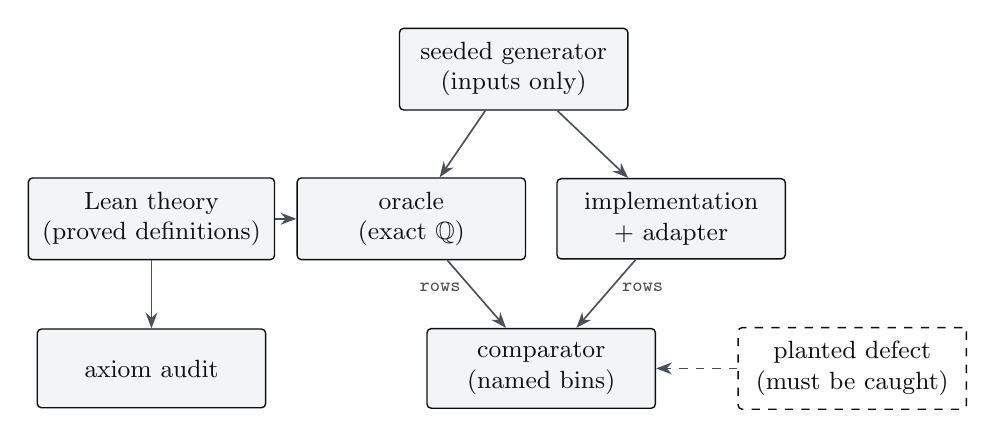
\begin{tikzpicture}[
  box/.style={draw=Ink, line width=0.5pt, fill=Surface, text=Ink, rounded corners=1.5pt,
    align=center, font=\small, inner sep=5pt, minimum height=10mm, minimum width=29mm},
  arr/.style={-{Stealth[length=2mm]}, line width=0.6pt, draw=InkMuted},
  lab/.style={font=\ttfamily\scriptsize, text=InkMuted}]
\node[box] (gen) at (4.6,1.9) {seeded generator\\(inputs only)};
\node[box] (theory) at (0,0) {Lean theory\\(proved definitions)};
\node[box] (oracle) at (3.3,0) {oracle\\(exact $\mathbb{Q}$)};
\node[box] (impl) at (6.6,0) {implementation\\+ adapter};
\node[box] (cmp) at (4.95,-1.9) {comparator\\(named bins)};
\node[box] (audit) at (0,-1.9) {axiom audit};
\node[box, dashed, fill=Background] (planted) at (8.9,-1.9) {planted defect\\(must be caught)};
\draw[arr] (gen) -- (oracle);
\draw[arr] (gen) -- (impl);
\draw[arr] (theory) -- (oracle);
\draw[arr] (theory) -- (audit);
\draw[arr] (oracle) -- node[left, lab, pos=0.4] {rows} (cmp);
\draw[arr] (impl) -- node[right, lab, pos=0.4] {rows} (cmp);
\draw[arr, dashed] (planted) -- (cmp);
\end{tikzpicture}
\caption{The measurement procedure. The generator never computes expected results;
those come only from the oracle.}
\label{fig:harness}
\end{figure}

The procedure follows \texttt{ledger-semantics} (\cref{fig:harness}). A seeded
generator writes case files containing inputs only. It favors the inputs where
implementations are known to have conventions: tied logits, words that are
themselves tokens, and merge tables with several splits of one string. A small
adapter per implementation runs the same cases and prints the oracle's row format.
The comparator places every case in exactly one named bin (agree, diverge, skipped
by either side, or missing), so nothing is dropped silently. Token rows are compared
as strings. Sampler rows require that a zero be matched by a zero and that nonzero
probabilities agree within $10^{-6}$, since llama.cpp stores logits in
\texttt{float32}. Each comparator is observed to fail: a planted defect, an adapter
that glues two tokens or one that inverts temperature, must be detected or the run
fails.

\paragraph{Tie divergences.} An implementation that keeps exactly $k$ tokens breaks
ties in its own order, which need not be the oracle's order by index. Every filter
treats tied tokens alike except for that choice, and tied tokens stay tied through
temperature and renormalization. Such an implementation must therefore agree with
the positional semantics up to a permutation of tied tokens. The harness checks
exactly this: the multiset of (logit, probability) pairs over the kept tokens must
equal that of the oracle's \texttt{q} rows. A divergence that fails this check is
reported as unexplained.

\begin{table}[t]
\centering\small
\caption{Measurements (\texttt{harness/run.sh 600}: four seeds of 600 cases each per
corpus). Lean 4.34.1, Mathlib v4.34.1, \texttt{tokenizers} 0.23.3, \texttt{tiktoken}
0.14.0, llama.cpp commit \texttt{a9d27ac} (2026-10-11).}
\label{tab:results}
\begin{tabularx}{\linewidth}{@{}>{\raggedright\arraybackslash}p{4.6cm}>{\raggedright\arraybackslash}X>{\raggedright\arraybackslash}X@{}}
\toprule
\qpth{Implementation} & \qpth{Compared against} & \qpth{Result}\\
\midrule
HF \texttt{tokenizers}, BPE, defaults & rule-rank BPE (\lean{bpe}) & 13{,}779 / 13{,}779 words identical\\
HF \texttt{tokenizers}, \lean{ignore_merges} & lookup, then rule-rank BPE & 13{,}779 / 13{,}779 identical\\
\texttt{tiktoken} & lookup, then concatenation-rank BPE & 13{,}779 / 13{,}779 identical\\
llama.cpp \lean{top_k}, \lean{top_p}, \lean{min_p}, \texttt{temp}, no ties & tie-keeping filters & 1{,}216 / 1{,}216 chains, $|\Delta p|\le5.1\times10^{-8}$\\
llama.cpp, with ties & tie-keeping, else positional & 939 + 245 / 1{,}184 chains; 0 unexplained\\
Planted defects (tokenizer, sampler) & --- & both detected\\
\bottomrule
\end{tabularx}
\end{table}

\Cref{tab:results} summarizes the results. Two findings came out of the
comparisons. First, \texttt{tiktoken} initially disagreed with the oracle's
concatenation-rank BPE on words that are themselves vocabulary tokens. The
disagreement was a convention, whole-word lookup. Following the
\texttt{ledger-semantics} rule that a divergence is either a defect in the
implementation or a convention the semantics has not yet recorded, we recorded it
as \lean{lookupFirst}, with its own theorems, after which agreement is exact.
Second, on the same random merge tables the two tokenizer libraries disagree with
each other on 439 of 13{,}779 words (3.2\%), and on 279 when Hugging Face uses
\lean{ignore_merges}. The oracle reproduces each library exactly, so every one of
these disagreements is predicted. \Cref{thm:bpeconv} states the condition under which
they cannot occur.

For sampling, llama.cpp agrees with the tie-keeping semantics on every tie-free
chain. On chains with ties, 245 of 1{,}184 diverge, and every one agrees with the
positional semantics up to a permutation of tied tokens. Some of these divergences
cascade: a tie cut by top-$k$ changes the renormalized masses that a later top-$p$
sees. A check that compared kept sets only after the fact would misclassify such
cases. Replaying the convention exactly classifies all of them.

% ===========================================================================
\section{Related work}

\paragraph{Formal methods for machine learning.} Most verification work on neural
networks proves properties of trained models, for example with SMT-based
methods~\cite{katz2017reluplex}. We verify the model-independent algorithms around
the model instead, and connect them to implementations through an oracle. The
denotational method follows Elliott~\cite{elliott2009denotational}. The use of a
proved semantics as a test oracle, the procedure of planted defects, and the
discipline of named skip bins follow \texttt{ledger-semantics}~\cite{ledgersemantics}.
Our category of finite stochastic maps is a special case of Fritz's Markov
categories~\cite{fritz2020markov}.

\paragraph{Tokenization.} Zouhar et al.\ give a formal analysis of BPE as an
optimization problem~\cite{zouhar2023bpe}. Gastaldi et al.\ treat tokenizers as
stochastic maps and study consistency of estimators~\cite{gastaldi2024foundations}.
Vieira et al.\ show how to turn token-level models into character-level
ones~\cite{vieira2024tokens}, which requires exactly the enumeration of
tokenizations we verify. Our no-compression theorem and the agreement criterion
between BPE conventions complement this work at the level of exact identities.

\paragraph{Decoding.} Top-$k$~\cite{fan2018hierarchical}, nucleus~\cite{holtzman2020curious}
and min-$p$~\cite{nguyen2025minp} sampling are usually specified by an algorithm over
sorted arrays, which leaves ties unspecified. \Cref{thm:topk} shows that this gap
cannot be closed by any symmetric rule. Speculative
sampling~\cite{leviathan2023speculative,chen2023speculative} is known to be lossless,
and its acceptance rate is the maximal-coupling bound~\cite{lindvall1992coupling}. Du et
al.\ characterize tightness measure-theoretically~\cite{du2023tight}. We give a
finite-depth statement and an explicit non-tight model.

\paragraph{Attention and inference systems.} Online softmax~\cite{milakov2018online}
underlies FlashAttention~\cite{dao2022flashattention} and its successors, and
KV caching is standard in serving systems~\cite{pope2023scaling,kwon2023vllm}. Our
contribution is the algebraic packaging, a commutative monoid with a free-monoid
homomorphism, and machine-checked proofs over arbitrary exponential characters.
Permutation equivariance of attention without positional encodings is
known~\cite{yun2020universal}.

\paragraph{Masked diffusion.} The time-independence of the optimal denoiser was
observed by Ou et al.~\cite{ou2025absorbing}, in the setting of
D3PM~\cite{austin2021d3pm}, MDLM~\cite{sahoo2024mdlm} and related
models~\cite{shi2024masked,nie2025llada}. We machine-check it, together with the
any-order chain rule and the inexactness of parallel unmasking.

% ===========================================================================
\section{Limitations}

Analysis on the reals enters only through exponential characters, and there is no
measure theory, so sampling and tightness are stated through finite quantities. The
oracle's temperature is restricted to $1/n$, which keeps softmax rational. The
theorems hold for every temperature, but the oracle cannot evaluate an irrational
softmax. Speculative decoding is proved for one drafted token. The sequence version
follows by induction and is not yet formalized. Nothing is proved about
floating-point arithmetic: implementations are compared with exact values within a
stated tolerance. A decision that lies exactly on a floating-point boundary could in
principle diverge, and none occurred in our runs. The diffusion theory covers
absorbing diffusion, not Gaussian diffusion. The chat protocol models tool calling in
its common request-and-result form, not any vendor's specification. The measurements
cover tokenizers and samplers; attention kernels, speculative decoders, chat
renderers and diffusion samplers are evaluated by the oracle but not yet compared
against implementations.

% ===========================================================================
\section{Conclusion}

The inference side of LLMs is small enough to be given a precise meaning and large
enough that its implementations disagree. A machine-checked semantics separates
what is meaning from what is convention. It proves which reorderings, cachings and
tilings are harmless, and it shows that some properties folklore expects, such as
symmetric exact top-$k$, compositional compressing tokenizers and unambiguous plain-text
templates, cannot exist. Connected to an exact oracle, the same definitions become
a test instrument. Every divergence it surfaces is either a defect in an
implementation or a convention that belongs in the semantics.

\paragraph{Availability.} The Lean development, oracle, harness, and recorded
measurement log accompany this paper.

\paragraph{Acknowledgments.} The structure of this work follows
\texttt{ledger-semantics} by John Wiegley. The formalization and harness were
developed with the assistance of an AI system (Claude, Anthropic).

% ===========================================================================
\begin{thebibliography}{99}\small

\bibitem{austin2021d3pm}
J.~Austin, D.~D. Johnson, J.~Ho, D.~Tarlow, and R.~van~den Berg.
\newblock Structured denoising diffusion models in discrete state-spaces.
\newblock In \emph{NeurIPS}, 2021.

\bibitem{chen2023speculative}
C.~Chen, S.~Borgeaud, G.~Irving, J.-B. Lespiau, L.~Sifre, and J.~Jumper.
\newblock Accelerating large language model decoding with speculative sampling.
\newblock arXiv:2302.01318, 2023.

\bibitem{dao2022flashattention}
T.~Dao, D.~Y. Fu, S.~Ermon, A.~Rudra, and C.~R{\'e}.
\newblock {FlashAttention}: Fast and memory-efficient exact attention with {IO}-awareness.
\newblock In \emph{NeurIPS}, 2022.

\bibitem{demoura2021lean4}
L.~de~Moura and S.~Ullrich.
\newblock The {Lean} 4 theorem prover and programming language.
\newblock In \emph{CADE-28}, 2021.

\bibitem{du2023tight}
L.~Du, L.~Torroba~Hennigen, T.~Pimentel, C.~Meister, J.~Eisner, and R.~Cotterell.
\newblock A measure-theoretic characterization of tight language models.
\newblock In \emph{ACL}, 2023.

\bibitem{elliott2009denotational}
C.~Elliott.
\newblock Denotational design with type class morphisms.
\newblock Technical Report 2009-01, LambdaPix, 2009.

\bibitem{fan2018hierarchical}
A.~Fan, M.~Lewis, and Y.~Dauphin.
\newblock Hierarchical neural story generation.
\newblock In \emph{ACL}, 2018.

\bibitem{fritz2020markov}
T.~Fritz.
\newblock A synthetic approach to {Markov} kernels, conditional independence and theorems on sufficient statistics.
\newblock \emph{Advances in Mathematics}, 370, 2020.

\bibitem{gastaldi2024foundations}
J.~L. Gastaldi, J.~Terilla, L.~Malagutti, B.~DuSell, T.~Vieira, and R.~Cotterell.
\newblock The foundations of tokenization: Statistical and computational concerns.
\newblock arXiv:2407.11606, 2024.

\bibitem{greshake2023injection}
K.~Greshake, S.~Abdelnabi, S.~Mishra, C.~Endres, T.~Holz, and M.~Fritz.
\newblock Not what you've signed up for: Compromising real-world {LLM}-integrated applications with indirect prompt injection.
\newblock In \emph{AISec}, 2023.

\bibitem{holtzman2020curious}
A.~Holtzman, J.~Buys, L.~Du, M.~Forbes, and Y.~Choi.
\newblock The curious case of neural text degeneration.
\newblock In \emph{ICLR}, 2020.

\bibitem{katz2017reluplex}
G.~Katz, C.~Barrett, D.~L. Dill, K.~Julian, and M.~J. Kochenderfer.
\newblock Reluplex: An efficient {SMT} solver for verifying deep neural networks.
\newblock In \emph{CAV}, 2017.

\bibitem{kwon2023vllm}
W.~Kwon, Z.~Li, S.~Zhuang, Y.~Sheng, L.~Zheng, C.~H. Yu, J.~E. Gonzalez, H.~Zhang, and I.~Stoica.
\newblock Efficient memory management for large language model serving with {PagedAttention}.
\newblock In \emph{SOSP}, 2023.

\bibitem{ledgersemantics}
J.~Wiegley.
\newblock ledger-semantics: Mathematical semantics of {Ledger}, the double-entry accounting tool.
\newblock \url{https://github.com/ledger/ledger-semantics}, 2026.

\bibitem{leviathan2023speculative}
Y.~Leviathan, M.~Kalman, and Y.~Matias.
\newblock Fast inference from transformers via speculative decoding.
\newblock In \emph{ICML}, 2023.

\bibitem{lindvall1992coupling}
T.~Lindvall.
\newblock \emph{Lectures on the Coupling Method}.
\newblock Wiley, 1992.

\bibitem{liu2023ring}
H.~Liu, M.~Zaharia, and P.~Abbeel.
\newblock Ring attention with blockwise transformers for near-infinite context.
\newblock arXiv:2310.01889, 2023.

\bibitem{mathlib2020}
The mathlib Community.
\newblock The {Lean} mathematical library.
\newblock In \emph{CPP}, 2020.

\bibitem{milakov2018online}
M.~Milakov and N.~Gimelshein.
\newblock Online normalizer calculation for softmax.
\newblock arXiv:1805.02867, 2018.

\bibitem{nguyen2025minp}
M.~N. Nguyen, A.~Baker, C.~Neo, A.~Roush, A.~Kirsch, and R.~Shwartz-Ziv.
\newblock Turning up the heat: Min-p sampling for creative and coherent {LLM} outputs.
\newblock In \emph{ICLR}, 2025.

\bibitem{nie2025llada}
S.~Nie, F.~Zhu, Z.~You, X.~Zhang, J.~Ou, J.~Hu, J.~Zhou, Y.~Lin, J.-R. Wen, and C.~Li.
\newblock Large language diffusion models.
\newblock arXiv:2502.09992, 2025.

\bibitem{ou2025absorbing}
J.~Ou, S.~Nie, K.~Xue, F.~Zhu, J.~Sun, Z.~Li, and C.~Li.
\newblock Your absorbing discrete diffusion secretly models the conditional distributions of clean data.
\newblock In \emph{ICLR}, 2025.

\bibitem{pope2023scaling}
R.~Pope, S.~Douglas, A.~Chowdhery, J.~Devlin, J.~Bradbury, J.~Heek, K.~Xiao, S.~Agrawal, and J.~Dean.
\newblock Efficiently scaling transformer inference.
\newblock In \emph{MLSys}, 2023.

\bibitem{rabe2021selfattention}
M.~N. Rabe and C.~Staats.
\newblock Self-attention does not need {$O(n^2)$} memory.
\newblock arXiv:2112.05682, 2021.

\bibitem{radford2019gpt2}
A.~Radford, J.~Wu, R.~Child, D.~Luan, D.~Amodei, and I.~Sutskever.
\newblock Language models are unsupervised multitask learners.
\newblock OpenAI technical report, 2019.

\bibitem{sahoo2024mdlm}
S.~S. Sahoo, M.~Arriola, Y.~Schiff, A.~Gokaslan, E.~Marroquin, J.~T. Chiu, A.~Rush, and V.~Kuleshov.
\newblock Simple and effective masked diffusion language models.
\newblock In \emph{NeurIPS}, 2024.

\bibitem{sennrich2016bpe}
R.~Sennrich, B.~Haddow, and A.~Birch.
\newblock Neural machine translation of rare words with subword units.
\newblock In \emph{ACL}, 2016.

\bibitem{shi2024masked}
J.~Shi, K.~Han, Z.~Wang, A.~Doucet, and M.~K. Titsias.
\newblock Simplified and generalized masked diffusion for discrete data.
\newblock In \emph{NeurIPS}, 2024.

\bibitem{vieira2024tokens}
T.~Vieira, B.~LeBrun, M.~Giulianelli, J.~L. Gastaldi, B.~DuSell, J.~Terilla, T.~J. O'Donnell, and R.~Cotterell.
\newblock From language models over tokens to language models over characters.
\newblock arXiv:2412.03719, 2024.

\bibitem{wolf2020transformers}
T.~Wolf et~al.
\newblock Transformers: State-of-the-art natural language processing.
\newblock In \emph{EMNLP: System Demonstrations}, 2020.

\bibitem{xiao2024sinks}
G.~Xiao, Y.~Tian, B.~Chen, S.~Han, and M.~Lewis.
\newblock Efficient streaming language models with attention sinks.
\newblock In \emph{ICLR}, 2024.

\bibitem{yun2020universal}
C.~Yun, S.~Bhojanapalli, A.~S. Rawat, S.~J. Reddi, and S.~Kumar.
\newblock Are transformers universal approximators of sequence-to-sequence functions?
\newblock In \emph{ICLR}, 2020.

\bibitem{zouhar2023bpe}
V.~Zouhar, C.~Meister, J.~L. Gastaldi, L.~Du, T.~Vieira, M.~Sachan, and R.~Cotterell.
\newblock A formal perspective on byte-pair encoding.
\newblock In \emph{Findings of ACL}, 2023.

\end{thebibliography}

\end{document}
"

\usepackage[a4paper,textwidth=15.4cm,textheight=23.6cm,top=3.0cm,headsep=0.9cm,footskip=1.2cm]{geometry}
\usepackage{amsmath,amssymb,amsthm,mathtools}
\usepackage{fontspec}
\usepackage{booktabs,tabularx,array}
\usepackage[protrusion=true,expansion=false]{microtype}
\usepackage[table]{xcolor}
\usepackage{graphicx}
\usepackage{fvextra}
\usepackage{enumitem}
\usepackage{caption}
\usepackage{titlesec}
\usepackage{fancyhdr}
\usepackage[most]{tcolorbox}
\usepackage{tikz}
\usetikzlibrary{arrows.meta}
\usepackage{hyperref}
\usepackage[nameinlink,capitalise]{cleveref}

% ---------------------------------------------------------------------------
%  Colour tokens
% ---------------------------------------------------------------------------
% Neutral foundation. Ink and Background invert between the two editions.
\ifqptdark
  \definecolor{Background}{HTML}{0B0C0E}
  \definecolor{Surface}{HTML}{16181B}
  \definecolor{Border}{HTML}{2B2E33}
  \definecolor{Ink}{HTML}{EDEEF0}
  \definecolor{InkMuted}{HTML}{A9AEB6}
  \definecolor{InkFaint}{HTML}{5A5F67}   % decoration only, never meaningful text
\else
  \definecolor{Background}{HTML}{FFFFFF}
  \definecolor{Surface}{HTML}{F3F4F5}
  \definecolor{Border}{HTML}{DADDE1}
  \definecolor{Ink}{HTML}{0E0F11}
  \definecolor{InkMuted}{HTML}{4B4F57}
  \definecolor{InkFaint}{HTML}{A3A7AE}   % decoration only, never meaningful text
\fi
% Paradigm colours: fixed in both editions, semantic only.
\definecolor{Quantum}{HTML}{5BAD1E}
\definecolor{Photonic}{HTML}{F0AB00}
\definecolor{Thermodynamic}{HTML}{E8690A}
\definecolor{Ternary}{HTML}{8A8A8A}
\definecolor{Bio}{HTML}{1AAB7C}

\ifqptdark\pagecolor{Background}\fi

% ---------------------------------------------------------------------------
%  Typography
% ---------------------------------------------------------------------------
\setmainfont{Inter}[
  Path=fonts/, Extension=.otf, Scale=0.94,
  UprightFont=*-Regular, ItalicFont=*-Italic,
  BoldFont=*-SemiBold, BoldItalicFont=*-SemiBoldItalic]
\setmonofont{IBMPlexMono}[
  Path=fonts/, Extension=.ttf, Scale=MatchLowercase,
  UprightFont=*-Regular, ItalicFont=*-Italic, BoldFont=*-SemiBold]
\newfontfamily\qptdisplay{SpaceGrotesk}[
  Path=fonts/, Extension=.otf, UprightFont=*-Medium, BoldFont=*-Bold]
\newfontfamily\qptdisplaylight{SpaceGrotesk}[
  Path=fonts/, Extension=.otf, UprightFont=*-Regular]
\newfontfamily\qptlabelfont{IBMPlexMono}[
  Path=fonts/, Extension=.ttf, Scale=MatchLowercase, UprightFont=*-Medium,
  LetterSpace=6]
\setsansfont{Inter}[
  Path=fonts/, Extension=.otf, Scale=0.94,
  UprightFont=*-Regular, ItalicFont=*-Italic,
  BoldFont=*-SemiBold, BoldItalicFont=*-SemiBoldItalic]
\linespread{1.16}
\setlength{\emergencystretch}{2.5em}
\AtBeginDocument{\raggedright\setlength{\parindent}{0pt}}
\setlength{\parindent}{0pt}
\setlength{\parskip}{0.55em}

% A label: IBM Plex Mono, upper case, tracked.
\newcommand{\qptlabel}[1]{{\qptlabelfont\footnotesize\MakeUppercase{#1}}}
% Technical names (Lean declarations, files) in IBM Plex Mono.
\newcommand{\lean}[1]{\texttt{\detokenize{#1}}}
\newcommand{\leanref}[1]{\par\smallskip\noindent
  {\ttfamily\footnotesize\upshape\raggedright\color{InkMuted}LEAN\enspace #1\par}}

% Ink is the normal colour everywhere, including floats, heads and footnotes.
\makeatletter
\AtBeginDocument{\color{Ink}\global\let\default@color\current@color}
\makeatother

% ---------------------------------------------------------------------------
%  Mathematical notation
% ---------------------------------------------------------------------------
\newcommand{\K}{\Bbbk}
\newcommand{\Dist}{\mathrm{Dist}}
\newcommand{\restr}[2]{#1|_{#2}}
\newcommand{\topk}{\mathrm{TopK}}
\newcommand{\topp}{\mathrm{TopP}}
\newcommand{\minp}{\mathrm{MinP}}
\newcommand{\sharpen}{\mathrm{sharpen}}
\newcommand{\abv}{\mathrm{above}}
\newcommand{\tv}{\mathrm{tv}}
\newcommand{\dec}{\mathrm{dec}}
\newcommand{\enc}{\mathrm{enc}}
\newcommand{\softmax}{\mathrm{softmax}}
\newcommand{\attend}{\mathrm{attend}}
\newcommand{\Iv}[1]{[\![#1]\!]}
\newcommand{\Mask}{\bot}

% ---------------------------------------------------------------------------
%  Headings: section numbers as labels, titles in Space Grotesk
% ---------------------------------------------------------------------------
\makeatletter
\newcommand{\qptsecnum}[1]{{\qptlabelfont\small\color{InkMuted}\two@digits{#1}}}
\makeatother
\titleformat{\section}
  {\qptdisplay\fontsize{14.5}{18}\selectfont\color{Ink}}
  {\qptsecnum{\value{section}}}{0.9em}{}
\titleformat{name=\section,numberless}
  {\qptdisplay\fontsize{14.5}{18}\selectfont\color{Ink}}{}{0pt}{}
\titlespacing*{\section}{0pt}{1.9em}{0.7em}
\titleformat{\paragraph}[runin]
  {\qptdisplay\normalsize\color{Ink}}{}{0pt}{}
\titlespacing*{\paragraph}{0pt}{0.9em}{0.6em}

% ---------------------------------------------------------------------------
%  Statements
% ---------------------------------------------------------------------------
\newtheoremstyle{qpt}
  {0.9em}{0.9em}
  {\normalfont}{}
  {\qptlabelfont\footnotesize}{}
  {\newline}
  {\MakeUppercase{\thmname{#1}\thmnumber{~#2}}%
   \thmnote{\enspace{\qptdisplay\normalsize\color{Ink}#3}}}
\theoremstyle{qpt}
\newtheorem{theorem}{Theorem}
\newtheorem{proposition}[theorem]{Proposition}
\newtheorem{corollary}[theorem]{Corollary}
\newtheorem{lemma}[theorem]{Lemma}
\newtheorem{definition}[theorem]{Definition}
\newtheorem{remark}[theorem]{Remark}

% Proofs: a tracked label and a neutral end mark.
\makeatletter
\renewcommand{\qedsymbol}{{\color{InkMuted}\rule{0.5em}{0.5em}}}
\renewenvironment{proof}[1][Proof]{\par\pushQED{\qed}\normalfont\topsep0.5em\relax
  \trivlist\item[\hskip\labelsep\qptlabel{#1}\hspace{0.6em}]\ignorespaces}
  {\popQED\endtrivlist\@endpefalse}
\makeatother

% ---------------------------------------------------------------------------
%  Code: IBM Plex Mono on a neutral surface, with a hairline on the left
% ---------------------------------------------------------------------------
\tcbset{colupper=Ink, collower=Ink}
\tcbset{qptcode/.style={enhanced, colback=Surface, colframe=Surface,
  boxrule=0pt, arc=0pt, left=9pt, right=8pt, top=5pt, bottom=5pt,
  borderline west={1.2pt}{0pt}{InkFaint}, before skip=0.7em, after skip=0.7em}}
\newenvironment{leancode}
  {\VerbatimEnvironment\begin{tcolorbox}[qptcode]%
   \begin{Verbatim}[fontsize=\small,commandchars=\\\{\},
     codes={\catcode`\$=3\catcode`\^=7},formatcom=\color{Ink}]}
  {\end{Verbatim}\end{tcolorbox}}
\newenvironment{casecode}
  {\VerbatimEnvironment\begin{tcolorbox}[qptcode,before skip=0pt,after skip=0pt]%
   \begin{Verbatim}[fontsize=\footnotesize,formatcom=\color{Ink}]}
  {\end{Verbatim}\end{tcolorbox}}

% ---------------------------------------------------------------------------
%  Floats, tables, captions
% ---------------------------------------------------------------------------
\DeclareCaptionLabelFormat{qpt}{\qptlabel{#1~#2}}
\DeclareCaptionLabelSeparator{qptsep}{\quad}
\captionsetup{labelformat=qpt, labelsep=qptsep, font={small,color=Ink},
  justification=raggedright, singlelinecheck=false, skip=6pt}
\newcommand{\qpth}[1]{\qptlabel{#1}}
\arrayrulecolor{Ink}
\setlength{\heavyrulewidth}{0.7pt}
\setlength{\lightrulewidth}{0.35pt}
\renewcommand{\arraystretch}{1.22}

% ---------------------------------------------------------------------------
%  Running heads
% ---------------------------------------------------------------------------
\pagestyle{fancy}
\fancyhf{}
\fancyhead[L]{{\color{Ink}\qptlabel{Machine-checked semantics of LLM inference}}}
\fancyhead[R]{{\color{Ink}\qptlabel{D. Arango Sohm}}}
\fancyfoot[R]{{\ttfamily\small\color{InkMuted}\thepage}}
\renewcommand{\headrule}{{\color{Border}\hrule height 0.4pt}\vspace{-0.4pt}}
\renewcommand{\headrulewidth}{0.4pt}
\fancypagestyle{qptfirst}{\fancyhf{}%
  \fancyfoot[R]{{\ttfamily\small\color{InkMuted}\thepage}}%
  \renewcommand{\headrulewidth}{0pt}\renewcommand{\headrule}{}}

% ---------------------------------------------------------------------------
%  Links and references: neutral, never accent-coloured text
% ---------------------------------------------------------------------------
\hypersetup{colorlinks=true, linkcolor=Ink, citecolor=Ink, urlcolor=Ink,
  pdftitle={A Machine-Checked Semantics of LLM Inference},
  pdfauthor={Daniel Arango Sohm},
  pdfsubject={Formal semantics of large language model inference in Lean 4},
  pdfkeywords={Lean 4, Mathlib, formal verification, LLM inference, sampling,
    tokenization, attention, speculative decoding, diffusion language models}}
\makeatletter
\renewcommand{\@biblabel}[1]{{\ttfamily\color{InkMuted}[#1]}}
\renewcommand{\@cite}[2]{{\ttfamily[#1\if@tempswa, #2\fi]}}
\makeatother
\renewcommand{\refname}{References}

\setlist{itemsep=2pt, topsep=4pt}
\setlist[itemize]{label={\color{InkMuted}\textbullet}}

\begin{document}
\thispagestyle{qptfirst}

% ----------------------------------------------------------------- masthead
\noindent
\begin{minipage}[c]{0.5\linewidth}
  \includegraphics[height=1.9cm]{qpt-logo.png}
\end{minipage}%
\begin{minipage}[c]{0.5\linewidth}\raggedleft
  \qptlabel{Preprint}\\[2pt]
  \qptlabel{October 2026}
\end{minipage}

\vspace{1.6em}
{\color{Border}\rule{\linewidth}{0.4pt}}
\vspace{1.1em}

{\qptdisplay\fontsize{25}{29.5}\selectfont\color{Ink}
A Machine-Checked Semantics\\ of LLM Inference\par}
\vspace{0.55em}
{\qptdisplaylight\fontsize{13}{17}\selectfont\color{InkMuted}
Sampling, Attention, Tokenization, Chat, Decoding,\\ and Diffusion in Lean~4\par}

\vspace{1.5em}
{\large\bfseries Daniel Arango Sohm}\par
\vspace{0.15em}
{\color{InkMuted}Universidad EAFIT, Medellín, Colombia\\
Former member of the QPT team}\par

\vspace{1.4em}
% ----------------------------------------------------------------- abstract
\begin{tcolorbox}[enhanced, colback=Surface, colframe=Surface, colupper=Ink, boxrule=0pt,
  arc=0pt, left=12pt, right=12pt, top=9pt, bottom=10pt]
\qptlabel{Abstract}\par\vspace{0.35em}
{\small
The inference side of a large language model is a stack of small algorithms:
tokenizers, attention kernels, key--value caches, sampling filters, speculative
decoders, chat templates, and diffusion samplers. Each has several independent
implementations, and those implementations are usually tested against one another
rather than against a definition. We give these components a single mathematical
semantics, formalized in Lean~4 against Mathlib. The development comprises about
4{,}600 lines and 270 named theorems, and every declaration depends only on Lean's
three standard axioms. It proves the exact algebra of sampling filters, the
losslessness and optimality of speculative sampling, and the correctness of
key--value caching and of FlashAttention-style online softmax as a commutative
monoid. It proves that byte-pair encoding is lossless under every merge priority,
together with a decidable criterion for when the Hugging Face and \texttt{tiktoken}
conventions agree, a protocol checker for tool calls, and the time-independence of
the masked-diffusion denoiser. It also proves six negative results. No sampling
rule that treats tokens symmetrically can always keep exactly $k$ tokens. No
tokenizer that compresses can respect concatenation. Every chat template that writes
its role markers in the content alphabet is ambiguous. No transformer without
positional information can copy a fixed position. An autoregressive model need not
define a distribution over strings. Parallel unmasking in diffusion is inexact.
From the same definitions we build an executable oracle that evaluates test cases in
exact rational arithmetic, and a harness that measures implementations against it.
On 2{,}400 random merge tables, Hugging Face \texttt{tokenizers} and
\texttt{tiktoken} each agree with the oracle on all 13{,}779 test words, while
disagreeing with each other on 3.2\% of them. On 2{,}400 random sampler chains,
every divergence of llama.cpp from the tie-keeping semantics is accounted for
exactly by the positional semantics that the impossibility theorem forces.
\par}
\end{tcolorbox}

\vspace{0.3em}
\noindent\qptlabel{Keywords}\enspace{\small Lean~4 · Mathlib · formal verification ·
LLM inference · sampling · tokenization · attention · speculative decoding ·
diffusion language models}

\vspace{0.4em}
{\color{Border}\rule{\linewidth}{0.4pt}}

% ===========================================================================
\section{Introduction}

A deployed language model is a function from parameters and a context to a
distribution over tokens. Turning that distribution into text requires more
machinery. A tokenizer maps strings to token sequences. Attention kernels compute
the model's reads over a cached context. A chain of sampling filters reshapes the
next-token distribution. A speculative decoder may verify drafted tokens, a chat
template linearizes a conversation, and a diffusion sampler may unmask several
positions at once. Each of these components exists in many implementations, such as
Hugging Face \texttt{transformers} and \texttt{tokenizers}~\cite{wolf2020transformers},
\texttt{tiktoken}, vLLM~\cite{kwon2023vllm}, and llama.cpp. Their tests mostly
compare one implementation with another, or with remembered behavior.

This paper follows a different discipline, \emph{denotational design}~\cite{elliott2009denotational}.
One first says precisely what a thing means, then requires every operation to
preserve that meaning, and lets the implementation be whatever the equations force
it to be. The approach is that of \texttt{ledger-semantics}~\cite{ledgersemantics},
which formalizes double-entry accounting in Lean and uses the result as a test oracle
for the C++ Ledger program. We apply it to LLM inference. A sampling filter means
conditioning a distribution on a set. A KV-cached decoder means causal attention over
the whole prefix. A FlashAttention kernel means a softmax-weighted average. A chat
template means an injective encoding of a transcript. The theorems state when an
implementation preserves that meaning, and several of them state that no
implementation can.

\paragraph{Contributions.}
\begin{itemize}[leftmargin=*,itemsep=2pt]
\item A Lean~4 formalization against Mathlib~\cite{mathlib2020,demoura2021lean4}
  of sampling, speculative decoding, softmax and attention, tokenization, chat
  transcripts, autoregressive decoding, and masked diffusion
  (\cref{sec:foundations,sec:sampling,sec:spec,sec:attention,sec:tokenization,sec:chat,sec:decoding,sec:diffusion}).
  All definitions are stated over an arbitrary linearly ordered field, so one proof
  covers the real numbers of the literature and the exact rationals of the oracle.
\item Positive results in a common framework. They include the algebra of
  sampling filters, the optimality of speculative sampling, an online-softmax
  commutative monoid, a generic correctness theorem for BPE with a decidable
  agreement criterion between the two conventions in use, a protocol checker for
  tool calls, and the any-order chain rule for masked diffusion.
\item Six negative results that explain design constraints visible across
  implementations (\cref{sec:negative}).
\item An executable oracle that evaluates case files under the proved
  definitions in exact arithmetic, and a measurement of Hugging Face
  \texttt{tokenizers}, \texttt{tiktoken}, and llama.cpp against it (\cref{sec:oracle,sec:measure}).
\end{itemize}

Several of the positive results are known: losslessness of speculative
sampling~\cite{leviathan2023speculative,chen2023speculative}, correctness of online
softmax~\cite{milakov2018online,dao2022flashattention}, time-independence of the
absorbing-diffusion posterior~\cite{ou2025absorbing}, and the role of permutation
equivariance~\cite{yun2020universal}. Our contribution for these is a machine-checked
statement in one framework, connected to an oracle. To our knowledge the
following are not stated elsewhere in the form given here: the impossibility of
symmetric exact top-$k$ and nucleus selection, the no-compression theorem for
homomorphic tokenizers, the ambiguity of every in-band chat template, and the
decidable agreement criterion between merge-rule and concatenation-rank BPE.

% ===========================================================================
\section{Method and trust base}\label{sec:method}

The development is a Lean~4 library (Lean 4.34.1, Mathlib v4.34.1) of eleven
theory modules and two executable modules (\cref{tab:modules}). It is built with
warnings promoted to errors, so an unproved theorem (\lean{sorry}) fails the build.
A separate audit program walks every declaration in the library, 853 in all, and
fails unless each depends only on propositional extensionality, the axiom of choice,
and quotient soundness. The audit has been observed to fail: a planted proof by
\lean{native_decide}, which introduces an auxiliary axiom trusting compiled code, is
rejected. The warnings-as-errors build alone does not catch it. Concrete
counterexamples are therefore proved by \lean{decide}, whose certificate the kernel
checks by evaluation.

\begin{table}[t]
\centering\small
\caption{Modules of the development. Lines and named theorems and lemmas per module.}
\label{tab:modules}
\begin{tabularx}{\linewidth}{@{}l>{\raggedright\arraybackslash}X>{\ttfamily}r>{\ttfamily}r@{}}
\toprule
\qpth{Module} & \qpth{Content} & \qpth{Lines} & \qpth{Thms} \\
\midrule
\lean{Dist} & finite distributions, conditioning, total variation, $\mathsf{FinStoch}$ & 383 & 34\\
\lean{Sampling} & top-$k$, top-$p$, min-$p$, temperature, ties, inverse CDF & 732 & 46\\
\lean{Counterexamples} & kernel-checked failures of sampler laws & 52 & 4\\
\lean{Speculative} & speculative sampling, couplings & 194 & 17\\
\lean{Softmax} & exponential characters, masking, temperature & 220 & 23\\
\lean{Attention} & equivariance, causality, KV cache, online softmax & 573 & 38\\
\lean{Real} & $\exp$ as a character; textbook restatements & 51 & 4\\
\lean{Tokenization} & free-monoid decoding, BPE conventions, enumeration & 860 & 49\\
\lean{Chat} & tool-call protocol, rendering & 440 & 21\\
\lean{Decoding} & mass conservation, tightness, greedy decoding & 245 & 15\\
\lean{Diffusion} & masked diffusion, posterior, chain rule & 379 & 18\\
\lean{Oracle}, \lean{Driver} & case parsing and exact evaluation & 465 & 1\\
\midrule
Total & & 4{,}594 & 270\\
\bottomrule
\end{tabularx}
\end{table}

\paragraph{Numbers.} Every probability lives in an arbitrary field $\K$ with a
compatible linear order (\lean{[Field K] [LinearOrder K] [IsStrictOrderedRing K]}).
The oracle instantiates $\K=\mathbb{Q}$, so its arithmetic is exact. The analytic
statements instantiate $\K=\mathbb{R}$. No measure theory is used. Sampling is made
precise through interval statements (\cref{thm:invcdf}), and tightness through
masses at finite depth (\cref{sec:decoding}).

% ===========================================================================
\section{Foundations}\label{sec:foundations}

\begin{definition}[Finite distribution]
For a finite type $\alpha$, $\Dist_\K(\alpha)$ is the type of functions
$p:\alpha\to\K$ with $p(a)\ge 0$ for all $a$ and $\sum_a p(a)=1$.
\leanref{\lean{Dist}}
\end{definition}

\begin{leancode}
structure Dist ($\K$ : Type u) [Field $\K$] [LinearOrder $\K$] [IsStrictOrderedRing $\K$]
    ($\alpha$ : Type v) [Fintype $\alpha$] where
  prob : $\alpha$ $\to$ $\K$
  nonneg : $\forall$ a, 0 $\le$ prob a
  sum_eq_one : $\sum$ a, prob a = 1
\end{leancode}

The single operation through which masks, filters and grammar constraints act is
conditioning. For $S\subseteq\alpha$ with $p(S)>0$, write
$\restr{p}{S}(a)=\Iv{a\in S}\,p(a)/p(S)$ (\lean{Dist.restrict}).

\begin{lemma}[Conditioning]\label{lem:restrict}
$\restr{(\restr{p}{S})}{T}=\restr{p}{S\cap T}$ whenever the masses involved are
positive. Moreover $\restr{p}{S}=\restr{p}{S'}$ whenever $S$ and $S'$ contain the same
outcomes of positive probability.
\leanref{\lean{restrict_restrict}, \lean{restrict_congr}}
\end{lemma}

The finite distribution monad (point masses and \lean{bind}) satisfies the monad
laws. Finite types and stochastic maps $\alpha\to\Dist_\K(\beta)$ form a category
$\mathsf{FinStoch}_\K$, given as an instance of Mathlib's \lean{Category} whose
composition is Kleisli composition (\lean{FinStoch.category}). Total variation is
$\tv(p,q)=\sum_a\max(0,p(a)-q(a))$. We prove
$\tv(p,q)=\tfrac12\sum_a|p(a)-q(a)|$, $\sum_a\min(p(a),q(a))=1-\tv(p,q)$, and
$\tv(p,q)=0\iff p=q$.

% ===========================================================================
\section{Sampling}\label{sec:sampling}

Let $V$ be a finite vocabulary and $p:V\to\K$. Write
$\abv_p(v)=\{u: p(v)<p(u)\}$ for the tokens strictly preferred to $v$. The three
standard filters keep the sets
\begin{gather*}
\topk_k(p)=\{v: |\abv_p(v)|<k\},\qquad
\minp_m(p)=\{v:\forall u,\; m\,p(u)\le p(v)\},\\
\topp_P(p)=\Bigl\{v: \textstyle\sum_{u\in\abv_p(v)}p(u)<P\Bigr\},
\end{gather*}
and the filtered distribution is the conditioning $\restr{p}{S}$ on the kept set
$S$. For distinct probabilities, $\topp_P$ is the usual rule ``sort in descending
order and keep the shortest prefix whose mass reaches $P$''. With ties, all three
keep every tied token. Temperature $1/n$ is
$\sharpen_n(p)(v)=p(v)^n/\sum_u p(u)^n$, which stays inside $\mathbb{Q}$. In
\cref{sec:attention} we show that it equals $\softmax(n\cdot z)$ when
$p=\softmax(z)$. Every kept set contains a most probable token, provided $k\ge1$,
$P>0$ and $m\le1$, so no filter can produce an empty distribution.

\begin{theorem}[Sampler algebra]\label{thm:algebra}
For $k,k'\ge1$, $m,m'\le1$ and $n\ge1$, and writing filters in the order they are
applied,
\begin{enumerate}[label=(\roman*),itemsep=1pt]
\item top-$k$ then top-$k'$ equals top-$\min(k,k')$;
\item min-$m$ then min-$m'$ equals min-$\max(m,m')$; in particular both filters are idempotent;
\item top-$k$ and min-$m$ commute;
\item top-$k$ and temperature $1/n$ commute.
\end{enumerate}
\leanref{\lean{topK_topK}, \lean{minP_minP}, \lean{topK_minP_comm}, \lean{topK_sharpen_comm}}
\end{theorem}

\begin{proof}[Proof sketch]
All three kept sets are \emph{upward closed}: if $v$ is kept and $p(v)<p(u)$, then
$u$ is kept. Conditioning on an upward-closed set $S$ leaves $\abv(v)$ unchanged for
$v\in S$ (\lean{above_restrict}), and min-$p$ is insensitive to conditioning on a set
that contains a maximizer (\lean{minP_restrict_iff}). Each identity then reduces,
through \cref{lem:restrict}, to an equality of kept sets. For (iv), $x\mapsto x^n$
is strictly increasing on $[0,\infty)$, and top-$k$ depends only on the order of the
scores (\lean{topKSet_congr}).
\end{proof}

The laws one might expect beyond \cref{thm:algebra} are false. With
$p_0=(\tfrac12,\tfrac3{10},\tfrac15)$, the kernel evaluates the following
(\lean{Counterexamples}).

\begin{proposition}[Failed laws]\label{prop:counter}
\leavevmode\vspace{-0.5\baselineskip}
\begin{enumerate}[label=(\roman*),itemsep=1pt]
\item Top-$p$ is not idempotent: one pass of $\topp_{3/5}$ gives token~1 the probability $\tfrac38$, and a second pass gives it~$0$.
\item Top-$p$ does not commute with top-$k$: top-$p$ then top-2 leaves token~1 at $\tfrac38$, while top-2 then top-$p$ removes it.
\item Top-$p$ does not commute with temperature $\tfrac12$: token~1 ends at $\tfrac9{34}$ in one order and at $0$ in the other.
\item Min-$p$ ($m=\tfrac12$) does not commute with temperature $\tfrac12$, with the same numbers.
\end{enumerate}
\end{proposition}

A sampler chain may therefore reorder top-$k$, min-$p$ and temperature only as
\cref{thm:algebra} allows, and may not move top-$p$ at all.

\paragraph{Ties.} Implementations differ on ties, and the difference is forced.
Call a selection rule $\mathrm{sel}:(V\to\K)\to\mathcal{P}(V)$ \emph{equivariant} if
$\mathrm{sel}(p\circ\sigma^{-1})=\sigma[\mathrm{sel}(p)]$ for every permutation
$\sigma$ of $V$, that is, if relabeling the tokens relabels the output.

\begin{theorem}[No symmetric exact top-$k$]\label{thm:topk}
Let $0<k<|V|$. No equivariant selection rule satisfies $|\mathrm{sel}(p)|=k$ for
every distribution $p$.
\leanref{\lean{no_equivariant_exact_topK}}
\end{theorem}
\begin{proof}
On the uniform distribution $u$ we have $u\circ\sigma^{-1}=u$ for every $\sigma$, so
$\mathrm{sel}(u)$ is invariant under all permutations. If it contains some $v$, then
for any $w$ the transposition $(v\,w)$ maps $v$ to $w$, so it contains $w$ too.
Hence $\mathrm{sel}(u)$ is either empty or all of $V$, and neither has $k$ elements.
\end{proof}

\begin{leancode}
theorem no_equivariant_exact_topK [DecidableEq V] \char123{}k : $\mathbb{N}$\char125{}
    (hk0 : 0 < k) (hkn : k < Fintype.card V)
    (sel : (V $\to$ $\K$) $\to$ Finset V) (hsel : Equivariant sel) :
    $\neg$ $\forall$ d : Dist $\K$ V, (sel d.prob).card = k
\end{leancode}

\begin{theorem}[No symmetric smallest nucleus]
Let $V$ be nonempty and $0<P\le1-1/|V|$. No equivariant rule returns, for every
distribution, a set of minimum cardinality among those of mass at least~$P$.
\leanref{\lean{no_equivariant_exact_nucleus}}
\end{theorem}

The tie-keeping filters are equivariant (\lean{topKSet_equivariant}). The other
option is to break ties by position. Define $u\prec_p v$ if $p(u)>p(v)$, or if
$p(u)=p(v)$ and $u<v$, and let the positional filters count predecessors under
$\prec_p$ instead of $\abv_p$ (\lean{Dist.topKPos}, \lean{Dist.topPPos}).

\begin{theorem}[Positional tie-breaking]
Positional top-$k$ keeps exactly $\min(k,|V|)$ tokens. If $p$ is injective, the
positional and tie-keeping filters coincide. For $0<k<|V|$, positional top-$k$ is
not equivariant.
\leanref{\lean{card_topKPosSet}, \lean{topKPosSet_eq_of_injective}, \lean{topPPosSet_eq_of_injective}, \lean{topKPosSet_not_equivariant}}
\end{theorem}

An implementation must therefore choose between keeping exactly $k$ tokens and
treating tokens symmetrically. Hugging Face \texttt{transformers} (read from the
source of version 5.19.0) keeps ties in top-$k$, since it removes only scores
strictly below the $k$-th largest, but breaks them by sort position in top-$p$.
llama.cpp breaks ties by position in both, as measured in \cref{sec:measure}.

\begin{theorem}[Inverse-CDF sampling]\label{thm:invcdf}
Let $F(i)=\sum_{j<i}p(j)$ on $V=\{0,\dots,n-1\}$ and let $\iota(u)$ be the least $i$
with $u<F(i+1)$. For $0\le u<1$, $\iota(u)=i\iff F(i)\le u<F(i+1)$, and
$F(i+1)-F(i)=p(i)$. A uniform $u$ therefore selects $i$ with probability $p(i)$.
\leanref{\lean{invCdf_eq_iff}, \lean{cdf_interval_length}}
\end{theorem}

% ===========================================================================
\section{Speculative decoding}\label{sec:spec}

A draft model proposes $x\sim q$. The target, with distribution $p$, accepts with
probability $a(x)=\min(1,p(x)/q(x))$, and on rejection a token is drawn from the
residual $r=(p-q)^+/\tv(p,q)$~\cite{leviathan2023speculative,chen2023speculative}.
We define the joint law of (draft, emitted token) exactly as the algorithm runs,
\[
\pi(x,y)=q(x)\bigl(a(x)\,\Iv{y=x}+(1-a(x))\,r(y)\bigr).
\]

\begin{theorem}[Speculative sampling]
\leavevmode\vspace{-0.5\baselineskip}
\begin{enumerate}[label=(\roman*),itemsep=1pt]
\item The draft has law $q$: $\sum_y\pi(x,y)=q(x)$.
\item \emph{Losslessness}: the emitted token has law $p$: $\sum_x\pi(x,y)=p(y)$.
\item The acceptance probability is $\sum_x q(x)a(x)=1-\tv(p,q)$, and the emitted token equals the draft with the same probability.
\item \emph{Optimality}: every coupling $\gamma$ of $q$ and $p$ has $\sum_x\gamma(x,x)\le1-\tv(p,q)$.
\end{enumerate}
\leanref{\lean{specJoint_fst}, \lean{specJoint_snd}, \lean{accept_rate}, \lean{specJoint_diag}, \lean{coupling_le}, \lean{spec_optimal}}
\end{theorem}
\begin{proof}[Proof sketch]
Since $q(x)a(x)=\min(p(x),q(x))$, the total rejection probability is $\tv(p,q)$,
and a rejected draft is never re-emitted, because $r(x)=0$ whenever $q(x)>p(x)$. For (iv),
$\gamma(x,x)\le\min(q(x),p(x))$ by the marginal constraints. This is the classical
coupling inequality~\cite{lindvall1992coupling}.
\end{proof}

Because any lossless rule for verifying one drafted token is a coupling, (iv) shows
that speculative sampling has the highest acceptance rate any such rule can achieve.

% ===========================================================================
\section{Softmax and attention}\label{sec:attention}

\begin{definition}[Exponential character]
An \emph{exponential character} from an ordered additive group $G$ of scores into
$\K$ is a strictly increasing map $E:G\to\K$ with $E(a)>0$ and $E(a+b)=E(a)E(b)$.
For $z:\iota\to G$, $\softmax_E(z)_i=E(z_i)/\sum_jE(z_j)$.
\leanref{\lean{ExpChar}}
\end{definition}

$\exp:\mathbb{R}\to\mathbb{R}$ is a character (\lean{ExpChar.real}). So is
$z\mapsto2^z:\mathbb{Z}\to\mathbb{Q}$ (\lean{ExpChar.base2}), which the oracle uses
to evaluate softmax with no rounding. Every result in this section holds for every
character, and so for both.

\begin{theorem}[Softmax]\label{thm:softmax}
\leavevmode\vspace{-0.5\baselineskip}
\begin{enumerate}[label=(\roman*),itemsep=1pt]
\item $\softmax_E(z+c)=\softmax_E(z)$; this licenses subtracting the maximum logit.
\item $\softmax_E(z)_i<\softmax_E(z)_j\iff z_i<z_j$.
\item \emph{Masking is conditioning}: setting logits outside $S$ to $-\infty$ and taking softmax gives $\restr{\softmax_E(z)}{S}$.
\item For $G$ a field and $T>0$, $\topk_k(\softmax_E(z/T))=\topk_k(z)$.
\item $\softmax_E(n\cdot z)=\sharpen_n(\softmax_E(z))$.
\end{enumerate}
\leanref{\lean{softmax_add_const}, \lean{softmax_lt_iff}, \lean{softmaxOn_eq_restrict}, \lean{topK_temperature}, \lean{softmax_nsmul}}
\end{theorem}

\paragraph{One read.} $\attend(s,v)=\sum_j\softmax_E(s)_j\,v_j$ for scores $s$ and
values $v_j$ in a $\K$-module.

\begin{theorem}[Convexity]
For every linear functional $\varphi$ and constant $c$, if $\varphi(v_j)\le c$ for all
$j$ then $\varphi(\attend(s,v))\le c$. If every $v_j=m$, then $\attend(s,v)=m$ for
every $s$.
\leanref{\lean{attend_convex}, \lean{attend_const}}
\end{theorem}

The second statement says attention cannot abstain. Its weights always sum to one,
which is the property that motivates attention-sink tokens~\cite{xiao2024sinks}.

\paragraph{Permutation equivariance.} A map $f:(\iota\to X)\to(\iota\to Y)$ is
equivariant if $f(x\circ\sigma)=f(x)\circ\sigma$ for every permutation~$\sigma$.

\begin{theorem}[Equivariance]
Self-attention with any score function and no positional information is
equivariant. So is any block $y=x+\sum_h\mathrm{attn}_h(\mathrm{norm}\,x)$,
$\mathrm{out}=y+\mathrm{mlp}(\mathrm{norm}\,y)$, and any stack of such blocks.
\leanref{\lean{selfAttn_equivariant}, \lean{block_equivariant}, \lean{stack_equivariant}}
\end{theorem}

\begin{theorem}[Positional information is necessary]\label{thm:nofirst}
If $\iota$ has two distinct positions $i_0\ne i_1$ and $X$ has two distinct elements,
no equivariant $f:(\iota\to X)\to(\iota\to X)$ satisfies $f(x)_i=x_{i_0}$ for all $x$ and $i$.
\leanref{\lean{no_equivariant_first}}
\end{theorem}
\begin{proof}
Let $x_{i_0}=a$ and $x_i=b$ elsewhere, and let $\sigma=(i_0\,i_1)$. Then
$f(x\circ\sigma)_{i_0}=(x\circ\sigma)_{i_0}=b$, while equivariance gives
$f(x\circ\sigma)_{i_0}=f(x)_{i_1}=x_{i_0}=a$.
\end{proof}

Without positional encodings, then, no transformer can output the token at a fixed
position~\cite{yun2020universal}.

\paragraph{Causality and the KV cache.} Causal attention over a list maps position
$i$ to a read with the query of $x_i$ over the keys and values of $x_0,\dots,x_i$
(\lean{causalAttn}). The cached decoder \lean{kvDecode} appends one (key, value) pair
per step and reads the cache, recomputing nothing.

\begin{theorem}[Causality and KV caching]
Causal attention is causal: it preserves length, and its output on a prefix is the
prefix of its output. Causal maps are closed under composition and residual sums.
\emph{KV caching is exact}: $\mathrm{kvDecode}(xs)=\mathrm{causalAttn}(xs)$. For any
causal $f$, $f(xs\mathbin{+\!\!+}[x])=f(xs)\mathbin{+\!\!+}(\text{last entry})$.
\leanref{\lean{causalAttn_causal}, \lean{kvDecode_eq}, \lean{causal_comp}, \lean{causal_extend}}
\end{theorem}

\paragraph{Online softmax as a monoid.} FlashAttention~\cite{dao2022flashattention},
memory-efficient attention~\cite{rabe2021selfattention} and ring
attention~\cite{liu2023ring} reduce attention over blocks of keys using the online
normalizer of Milakov and Gimelshein~\cite{milakov2018online}. A partial state is a
triple $(m,\ell,o)$ of running maximum, normalizer and accumulator, and two states
merge by rescaling to the larger maximum:
\[
(m_1,\ell_1,o_1)\otimes(m_2,\ell_2,o_2)=
\bigl(m,\;\ell_1E(m_1-m)+\ell_2E(m_2-m),\;E(m_1-m)\,o_1+E(m_2-m)\,o_2\bigr),
\]
where $m=\max(m_1,m_2)$.

\begin{theorem}[Online softmax]
Adjoining an identity for the empty block, $\otimes$ is a commutative monoid. Let
$\mathrm{single}(s,v)=(s,1,v)$ and $\mathrm{fin}(m,\ell,o)=\ell^{-1}o$. For every
list of (score, value) pairs, $\mathrm{fin}\bigl(\prod_j\mathrm{single}(s_j,v_j)\bigr)
=\bigl(\sum_jE(s_j)\bigr)^{-1}\sum_jE(s_j)v_j$. The same holds for every partition
of the list into blocks and every order of the blocks. The running maximum of a
nonempty product is the maximum score, so every exponent the kernel evaluates is
$\le0$.
\leanref{\lean{Online}, \lean{finalize_ofList}, \lean{finalize_blocks}, \lean{ofList_perm}, \lean{ofList_max}}
\end{theorem}

The fold is the free-monoid homomorphism that \lean{single} induces
(\lean{ofList_eq_lift}). Correctness of tiling is then a homomorphism property
rather than a calculation.

% ===========================================================================
\section{Tokenization}\label{sec:tokenization}

A token $t$ spells a string $\mathrm{str}(t)$ over an alphabet $C$. Decoding is the
free-monoid homomorphism $\dec:T^*\to C^*$ that $\mathrm{str}$ induces
(\lean{decodeHom}).

\begin{theorem}[No compression]\label{thm:nocompress}
Suppose every token spells a nonempty string. If $\enc:C^*\to T^*$ satisfies
$\dec\circ\enc=\mathrm{id}$ and $\enc(a\,b)=\enc(a)\,\enc(b)$, then
$|\enc(s)|=|s|$ for every $s$, and every emitted token spells a single character.
Consequently, any tokenizer with $|\enc(s)|<|s|$ for some $s$ violates
$\enc(a\,b)=\enc(a)\,\enc(b)$ for some $a,b$.
\leanref{\lean{homomorphic_no_compression}, \lean{compressing_not_homomorphic}}
\end{theorem}
\begin{proof}[Proof sketch]
$\enc([c])$ is nonempty and decodes to $[c]$. Since each token decodes to at least
one character, it consists of exactly one token. Induct on $s$ using
$\enc(c\,s)=\enc([c])\,\enc(s)$.
\end{proof}

Tokenization therefore lies outside any compositional core, and boundary artifacts
such as the prompt-boundary problem are consequences of compression rather than
defects of one implementation. Tokenizations are not unique (\lean{decode_not_injective}).
\lean{tokenizations} enumerates every token sequence over a vocabulary that spells a
given string, and it is proved sound, complete and duplicate-free
(\lean{tokenizations_spec}, \lean{tokenizations_nodup}). The probability of a string
under a token-level model is the sum over this enumeration~\cite{vieira2024tokens,gastaldi2024foundations}.

\paragraph{BPE, generically.} Byte-pair
encoding~\cite{sennrich2016bpe,radford2019gpt2,zouhar2023bpe} repeatedly merges the
leftmost occurrence of the lowest-priority adjacent pair. We define it once, for an
arbitrary priority $f:T\times T\to\mathrm{Option}(\mathbb{N}\times T)$ that returns
a rank and a merged token (\lean{bpeWith}).

\begin{theorem}[Generic BPE]
Each step merges a pair of minimum rank, and every pair to its left has strictly
larger rank. The output contains no mergeable pair. BPE is idempotent. If $f$ is
\emph{sound}, meaning a merged token spells the concatenation of its parts, then BPE
is lossless.
\leanref{\lean{stepWith_spec}, \lean{bpeWith_normal}, \lean{bpeWith_idem}, \lean{bpeWith_decode}}
\end{theorem}

Two priorities are in use. Hugging Face \texttt{tokenizers} and the GPT-2 encoder
rank a pair by its merge \emph{rule} (\lean{rankOf}). \texttt{tiktoken} ranks a pair
by the rank of the \emph{token it would form} (\lean{concatRank}).

\begin{theorem}[Agreement of conventions]\label{thm:bpeconv}
Let $\mathcal{T}$ be a set of tokens closed under merging. If two priorities agree
on every pair from $\mathcal{T}$, their BPE outputs agree on every sequence over
$\mathcal{T}$. For a finite vocabulary this condition is decidable. Without it the
conventions differ: for the merges $(b,c),(a,b),(ab,c)$, the word $abc$ encodes as
$a\cdot bc$ under rule ranks and as $abc$ under concatenation ranks.
\leanref{\lean{bpeWith_congr}, \lean{hf_eq_tiktoken}, \lean{hf_ne_tiktoken}}
\end{theorem}

\texttt{tiktoken} also emits a word directly when the word is itself a vocabulary
token, and Hugging Face does the same with \lean{ignore_merges}. We record this
convention as \lean{lookupFirst}. It preserves losslessness (\lean{tikEncode_flatten})
and changes results (\lean{lookup_matters}). Finally, BPE does not find the shortest
tokenization (\lean{bpe_not_shortest}).

% ===========================================================================
\section{Chat transcripts}\label{sec:chat}

A transcript is a list of events: system, user and assistant messages,
$\mathrm{call}_i$ (a tool call with identifier $i$), and $\mathrm{result}_i$. Let
$c_i(\mathit{pre})$ and $r_i(\mathit{pre})$ count the calls and results with
identifier $i$, and let $\mathrm{NoPending}(\mathit{pre})$ mean $r_i=c_i$ for all
$i$. The protocol is stated per event, against the events before it.
\[
\mathrm{Allowed}(\mathit{pre},e)=
\begin{cases}
c_i(\mathit{pre})=0\wedge(\mathrm{NoPending}(\mathit{pre})\vee\mathrm{lastIsCall}(\mathit{pre})) & e=\mathrm{call}_i\\
c_i(\mathit{pre})=1\wedge r_i(\mathit{pre})=0 & e=\mathrm{result}_i\\
\mathrm{NoPending}(\mathit{pre}) & \text{otherwise.}
\end{cases}
\]
A transcript $es$ is \emph{valid} if every $es_k$ is allowed after $es_{<k}$.

\begin{theorem}[Protocol checker]
A single left-to-right pass with a state of (called, answered, last-was-call)
accepts exactly the valid transcripts. In a valid transcript every identifier is
called at most once and answered at most as often as it is called, and every result
is preceded by its call.
\leanref{\lean{check_iff_valid}, \lean{valid_counts}, \lean{result_has_call}}
\end{theorem}

Rendering with out-of-band markers, special symbols disjoint from content, is
invertible (\lean{parse_render}), and stays injective through any injective tokenizer
(\lean{render_encode_injective}). An \emph{in-band} template writes each event as
$\mathrm{open}(h)\,\mathit{body}\,\mathrm{close}$ with
$\mathrm{open}(h),\mathrm{close}\in C^*$.

\begin{theorem}[In-band ambiguity]\label{thm:inband}
For every choice of $\mathrm{open}$ and $\mathrm{close}$, in-band rendering is not
injective.
\leanref{\lean{inBand_not_injective}}
\end{theorem}
\begin{proof}
The single user message with body $\mathrm{close}\cdot\mathrm{open}(\mathrm{assistant})$
and the pair (empty user message, empty assistant message) both render to
$\mathrm{open}(\mathrm{user})\,\mathrm{close}\,\mathrm{open}(\mathrm{assistant})\,\mathrm{close}$.
\end{proof}

Role separation exists only at the token level, and only while user text cannot
produce a special token. This is the formal content behind the use of reserved tokens
as a defense against prompt injection~\cite{greshake2023injection}.

% ===========================================================================
\section{Autoregressive decoding}\label{sec:decoding}

A model assigns each prefix a distribution $m(\mathit{pre})\in\Dist_\K(V\cup\{\mathrm{eos}\})$.
Let $\mathrm{alive}_n$ be the probability of having generated $n$ tokens without
stopping, and $\mathrm{stopped}_n$ the probability of having stopped within~$n$.

\begin{theorem}[Mass conservation and tightness]
$\mathrm{stopped}_n+\mathrm{alive}_n=1$ for every $n$ and every starting prefix. If
every prefix stops with probability at least $\varepsilon$, then
$\mathrm{alive}_n\le(1-\varepsilon)^n$.
\leanref{\lean{mass_conservation}, \lean{alive_le_of_stop}}
\end{theorem}

\begin{theorem}[A non-tight model]\label{thm:leaky}
For the model that stops after $L$ tokens with probability $1/(L+2)^2$,
$\mathrm{alive}_n=\frac{n+2}{2(n+1)}$, so $\mathrm{stopped}_n<\frac12$ for every $n$.
\leanref{\lean{leaky_aliveMass}, \lean{stopped_lt_half}}
\end{theorem}

This model never places half of its probability on finite strings, so an
autoregressive model need not define a distribution over strings, the phenomenon
studied as tightness by Du et al.~\cite{du2023tight}.

\begin{theorem}[Greedy is not MAP]
There is a two-step model whose strictly most probable first token begins only
sequences of probability $\tfrac3{10}$, while another sequence has probability $\tfrac25$.
\leanref{\lean{greedy_not_map}}
\end{theorem}

Greedy decoding therefore does not find the most probable sequence, under any
tie-breaking.

% ===========================================================================
\section{Masked diffusion}\label{sec:diffusion}

Masked (absorbing) diffusion~\cite{austin2021d3pm,sahoo2024mdlm,shi2024masked,nie2025llada}
replaces each token, independently, with a mask symbol $\Mask$. The forward kernel
at keep rate $\alpha$ sends $v$ to $v$ with probability $\alpha$ and to $\Mask$ with
probability $1-\alpha$, and fixes $\Mask$.

\begin{theorem}[Forward process]
$\alpha\mapsto\mathrm{mask}_\alpha$ is a monoid homomorphism from the multiplicative
interval $[0,1]$ into the endomorphisms of $V\cup\{\Mask\}$ in $\mathsf{FinStoch}_\K$,
given as a Mathlib \lean{MonoidHom}. The sequence-level forward probability is
$q_\alpha(y\mid x)=\Iv{x\models y}\,(1-\alpha)^{\#\Mask(y)}\alpha^{n-\#\Mask(y)}$,
where $x\models y$ means $y$ agrees with $x$ wherever it is unmasked.
\leanref{\lean{forward}, \lean{maskProb_comp}, \lean{qSeq_closed}}
\end{theorem}

\begin{theorem}[Time-independent denoiser]\label{thm:timeindep}
For every data distribution $p$, every masked sequence $y$ and every $0<\alpha<1$,
\[
\frac{p(x)\,q_\alpha(y\mid x)}{\sum_{x'}p(x')\,q_\alpha(y\mid x')}
=\frac{\Iv{x\models y}\,p(x)}{\sum_{x'}\Iv{x'\models y}\,p(x')}.
\]
\leanref{\lean{posterior_time_independent}}
\end{theorem}

The optimal denoiser is therefore the data distribution conditioned on the unmasked
tokens, whatever the noise level, as observed by Ou et al.~\cite{ou2025absorbing}. The
factor that depends on $\alpha$ depends only on the mask pattern of $y$, and it
cancels. The closed-form reverse step used by samplers is the Bayes posterior of
the forward process (\lean{reverse_bayes}).

\begin{theorem}[Any-order chain rule]
Let $o_1,\dots,o_n$ enumerate the positions, and let $c_k$ be the exact conditional
probability that position $o_k$ holds $x_{o_k}$ given $x$ on $o_1,\dots,o_{k-1}$, with
$0/0=0$. Then $p(x)=\prod_kc_k$, and $c_k$ is the marginal of the posterior of
\cref{thm:timeindep} at $o_k$.
\leanref{\lean{chain_rule_fin}, \lean{posterior_marginal}}
\end{theorem}

Unmasking one position at a time with the exact denoiser therefore samples the data
distribution exactly, in every order.

\begin{proposition}[Parallel unmasking is inexact]
For the distribution uniform on $\{(0,1),(1,0)\}$, the product of the two exact
posterior marginals from the fully masked sequence gives $(1,1)$ the probability
$\tfrac14$, but $p(1,1)=0$.
\leanref{\lean{parallel_decoding_inexact}}
\end{proposition}

% ===========================================================================
\section{The negative results together}\label{sec:negative}

The six impossibility theorems share a shape. Each says that a property folklore
expects of a component is inconsistent with that component's purpose, and so each
explains a design constraint found in mature implementations.

\begin{enumerate}[label=(\arabic*),itemsep=2pt]
\item \emph{Symmetric exact top-$k$ does not exist} (\cref{thm:topk}). Every sampler must document its tie convention.
\item \emph{Compressing tokenizers are not compositional} (\cref{thm:nocompress}). Tokenization cannot be done piecewise, and prompt boundaries matter.
\item \emph{In-band chat templates are ambiguous} (\cref{thm:inband}). Roles require out-of-band special tokens.
\item \emph{Order requires positional information} (\cref{thm:nofirst}). Positional encodings are necessary, not an optimization.
\item \emph{Autoregressive models need not be tight} (\cref{thm:leaky}). Sequence-level probabilities need a stopping guarantee.
\item \emph{Parallel unmasking is inexact} (\cref{sec:diffusion}). Multi-token diffusion steps trade fidelity for speed.
\end{enumerate}

% ===========================================================================
\section{The oracle}\label{sec:oracle}

The oracle (\lean{LLM/Oracle.lean}, \lean{LLM/Driver.lean}) reads case files and
prints rows computed by the proved definitions over $\mathbb{Q}$. It runs under the
Lean interpreter (\texttt{lake env lean --run LLM/Driver.lean FILE}), so what
executes is a direct reading of the checked definitions. Inputs are validated at
run time, for example that probabilities are nonnegative and sum to one. The checks
are decidable propositions whose proofs construct the values the theorems speak
about.

\begin{figure}[t]
\begin{minipage}[t]{0.43\linewidth}
\begin{casecode}
@sample top-p is not idempotent
probs 1/2 3/10 1/5
top-p 3/5
emit
top-p 3/5
\end{casecode}
\end{minipage}\hfill
\begin{minipage}[t]{0.53\linewidth}
\begin{casecode}
-- top-p is not idempotent
p|0|5/8   p|1|3/8   p|2|0
q|0|5/8   q|1|3/8   q|2|0
p|0|1     p|1|0     p|2|0
q|0|1     q|1|0     q|2|0
\end{casecode}
\end{minipage}
\caption{A case file and the oracle's output, with rows placed side by side here.
Rows \texttt{p} use the tie-keeping filters and rows \texttt{q} the positional ones.
Every number is an exact rational.}
\label{fig:oracle}
\end{figure}

There are six case kinds. \texttt{@sample} runs a filter chain from probabilities,
weights, or integer logits under the base-2 softmax, and prints both tie
semantics (\cref{fig:oracle}). \texttt{@speculative} prints the acceptance rate,
total variation, per-token acceptance, residual, and emitted law. \texttt{@bpe}
prints the tokens under rule ranks, under rule ranks with whole-word lookup, and
under \texttt{tiktoken}'s convention, the number of tokenizations, and whether the
hypotheses of \cref{thm:bpeconv} hold. \texttt{@chat} prints validity with the first
offending event, and completeness. \texttt{@attention} prints softmax weights and
outputs, also through the online-softmax monoid over blocks. \texttt{@diffusion}
prints the evidence, posterior, and posterior marginals. A rejected case prints a
single \texttt{!!~ERROR} line.

% ===========================================================================
\section{Measuring implementations}\label{sec:measure}

\begin{figure}[t]
\centering
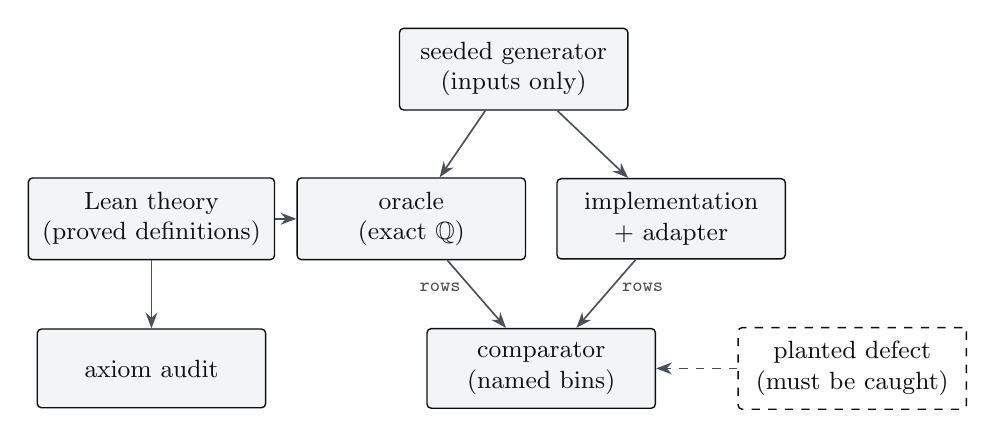
\begin{tikzpicture}[
  box/.style={draw=Ink, line width=0.5pt, fill=Surface, text=Ink, rounded corners=1.5pt,
    align=center, font=\small, inner sep=5pt, minimum height=10mm, minimum width=29mm},
  arr/.style={-{Stealth[length=2mm]}, line width=0.6pt, draw=InkMuted},
  lab/.style={font=\ttfamily\scriptsize, text=InkMuted}]
\node[box] (gen) at (4.6,1.9) {seeded generator\\(inputs only)};
\node[box] (theory) at (0,0) {Lean theory\\(proved definitions)};
\node[box] (oracle) at (3.3,0) {oracle\\(exact $\mathbb{Q}$)};
\node[box] (impl) at (6.6,0) {implementation\\+ adapter};
\node[box] (cmp) at (4.95,-1.9) {comparator\\(named bins)};
\node[box] (audit) at (0,-1.9) {axiom audit};
\node[box, dashed, fill=Background] (planted) at (8.9,-1.9) {planted defect\\(must be caught)};
\draw[arr] (gen) -- (oracle);
\draw[arr] (gen) -- (impl);
\draw[arr] (theory) -- (oracle);
\draw[arr] (theory) -- (audit);
\draw[arr] (oracle) -- node[left, lab, pos=0.4] {rows} (cmp);
\draw[arr] (impl) -- node[right, lab, pos=0.4] {rows} (cmp);
\draw[arr, dashed] (planted) -- (cmp);
\end{tikzpicture}
\caption{The measurement procedure. The generator never computes expected results;
those come only from the oracle.}
\label{fig:harness}
\end{figure}

The procedure follows \texttt{ledger-semantics} (\cref{fig:harness}). A seeded
generator writes case files containing inputs only. It favors the inputs where
implementations are known to have conventions: tied logits, words that are
themselves tokens, and merge tables with several splits of one string. A small
adapter per implementation runs the same cases and prints the oracle's row format.
The comparator places every case in exactly one named bin (agree, diverge, skipped
by either side, or missing), so nothing is dropped silently. Token rows are compared
as strings. Sampler rows require that a zero be matched by a zero and that nonzero
probabilities agree within $10^{-6}$, since llama.cpp stores logits in
\texttt{float32}. Each comparator is observed to fail: a planted defect, an adapter
that glues two tokens or one that inverts temperature, must be detected or the run
fails.

\paragraph{Tie divergences.} An implementation that keeps exactly $k$ tokens breaks
ties in its own order, which need not be the oracle's order by index. Every filter
treats tied tokens alike except for that choice, and tied tokens stay tied through
temperature and renormalization. Such an implementation must therefore agree with
the positional semantics up to a permutation of tied tokens. The harness checks
exactly this: the multiset of (logit, probability) pairs over the kept tokens must
equal that of the oracle's \texttt{q} rows. A divergence that fails this check is
reported as unexplained.

\begin{table}[t]
\centering\small
\caption{Measurements (\texttt{harness/run.sh 600}: four seeds of 600 cases each per
corpus). Lean 4.34.1, Mathlib v4.34.1, \texttt{tokenizers} 0.23.3, \texttt{tiktoken}
0.14.0, llama.cpp commit \texttt{a9d27ac} (2026-10-11).}
\label{tab:results}
\begin{tabularx}{\linewidth}{@{}>{\raggedright\arraybackslash}p{4.6cm}>{\raggedright\arraybackslash}X>{\raggedright\arraybackslash}X@{}}
\toprule
\qpth{Implementation} & \qpth{Compared against} & \qpth{Result}\\
\midrule
HF \texttt{tokenizers}, BPE, defaults & rule-rank BPE (\lean{bpe}) & 13{,}779 / 13{,}779 words identical\\
HF \texttt{tokenizers}, \lean{ignore_merges} & lookup, then rule-rank BPE & 13{,}779 / 13{,}779 identical\\
\texttt{tiktoken} & lookup, then concatenation-rank BPE & 13{,}779 / 13{,}779 identical\\
llama.cpp \lean{top_k}, \lean{top_p}, \lean{min_p}, \texttt{temp}, no ties & tie-keeping filters & 1{,}216 / 1{,}216 chains, $|\Delta p|\le5.1\times10^{-8}$\\
llama.cpp, with ties & tie-keeping, else positional & 939 + 245 / 1{,}184 chains; 0 unexplained\\
Planted defects (tokenizer, sampler) & --- & both detected\\
\bottomrule
\end{tabularx}
\end{table}

\Cref{tab:results} summarizes the results. Two findings came out of the
comparisons. First, \texttt{tiktoken} initially disagreed with the oracle's
concatenation-rank BPE on words that are themselves vocabulary tokens. The
disagreement was a convention, whole-word lookup. Following the
\texttt{ledger-semantics} rule that a divergence is either a defect in the
implementation or a convention the semantics has not yet recorded, we recorded it
as \lean{lookupFirst}, with its own theorems, after which agreement is exact.
Second, on the same random merge tables the two tokenizer libraries disagree with
each other on 439 of 13{,}779 words (3.2\%), and on 279 when Hugging Face uses
\lean{ignore_merges}. The oracle reproduces each library exactly, so every one of
these disagreements is predicted. \Cref{thm:bpeconv} states the condition under which
they cannot occur.

For sampling, llama.cpp agrees with the tie-keeping semantics on every tie-free
chain. On chains with ties, 245 of 1{,}184 diverge, and every one agrees with the
positional semantics up to a permutation of tied tokens. Some of these divergences
cascade: a tie cut by top-$k$ changes the renormalized masses that a later top-$p$
sees. A check that compared kept sets only after the fact would misclassify such
cases. Replaying the convention exactly classifies all of them.

% ===========================================================================
\section{Related work}

\paragraph{Formal methods for machine learning.} Most verification work on neural
networks proves properties of trained models, for example with SMT-based
methods~\cite{katz2017reluplex}. We verify the model-independent algorithms around
the model instead, and connect them to implementations through an oracle. The
denotational method follows Elliott~\cite{elliott2009denotational}. The use of a
proved semantics as a test oracle, the procedure of planted defects, and the
discipline of named skip bins follow \texttt{ledger-semantics}~\cite{ledgersemantics}.
Our category of finite stochastic maps is a special case of Fritz's Markov
categories~\cite{fritz2020markov}.

\paragraph{Tokenization.} Zouhar et al.\ give a formal analysis of BPE as an
optimization problem~\cite{zouhar2023bpe}. Gastaldi et al.\ treat tokenizers as
stochastic maps and study consistency of estimators~\cite{gastaldi2024foundations}.
Vieira et al.\ show how to turn token-level models into character-level
ones~\cite{vieira2024tokens}, which requires exactly the enumeration of
tokenizations we verify. Our no-compression theorem and the agreement criterion
between BPE conventions complement this work at the level of exact identities.

\paragraph{Decoding.} Top-$k$~\cite{fan2018hierarchical}, nucleus~\cite{holtzman2020curious}
and min-$p$~\cite{nguyen2025minp} sampling are usually specified by an algorithm over
sorted arrays, which leaves ties unspecified. \Cref{thm:topk} shows that this gap
cannot be closed by any symmetric rule. Speculative
sampling~\cite{leviathan2023speculative,chen2023speculative} is known to be lossless,
and its acceptance rate is the maximal-coupling bound~\cite{lindvall1992coupling}. Du et
al.\ characterize tightness measure-theoretically~\cite{du2023tight}. We give a
finite-depth statement and an explicit non-tight model.

\paragraph{Attention and inference systems.} Online softmax~\cite{milakov2018online}
underlies FlashAttention~\cite{dao2022flashattention} and its successors, and
KV caching is standard in serving systems~\cite{pope2023scaling,kwon2023vllm}. Our
contribution is the algebraic packaging, a commutative monoid with a free-monoid
homomorphism, and machine-checked proofs over arbitrary exponential characters.
Permutation equivariance of attention without positional encodings is
known~\cite{yun2020universal}.

\paragraph{Masked diffusion.} The time-independence of the optimal denoiser was
observed by Ou et al.~\cite{ou2025absorbing}, in the setting of
D3PM~\cite{austin2021d3pm}, MDLM~\cite{sahoo2024mdlm} and related
models~\cite{shi2024masked,nie2025llada}. We machine-check it, together with the
any-order chain rule and the inexactness of parallel unmasking.

% ===========================================================================
\section{Limitations}

Analysis on the reals enters only through exponential characters, and there is no
measure theory, so sampling and tightness are stated through finite quantities. The
oracle's temperature is restricted to $1/n$, which keeps softmax rational. The
theorems hold for every temperature, but the oracle cannot evaluate an irrational
softmax. Speculative decoding is proved for one drafted token. The sequence version
follows by induction and is not yet formalized. Nothing is proved about
floating-point arithmetic: implementations are compared with exact values within a
stated tolerance. A decision that lies exactly on a floating-point boundary could in
principle diverge, and none occurred in our runs. The diffusion theory covers
absorbing diffusion, not Gaussian diffusion. The chat protocol models tool calling in
its common request-and-result form, not any vendor's specification. The measurements
cover tokenizers and samplers; attention kernels, speculative decoders, chat
renderers and diffusion samplers are evaluated by the oracle but not yet compared
against implementations.

% ===========================================================================
\section{Conclusion}

The inference side of LLMs is small enough to be given a precise meaning and large
enough that its implementations disagree. A machine-checked semantics separates
what is meaning from what is convention. It proves which reorderings, cachings and
tilings are harmless, and it shows that some properties folklore expects, such as
symmetric exact top-$k$, compositional compressing tokenizers and unambiguous plain-text
templates, cannot exist. Connected to an exact oracle, the same definitions become
a test instrument. Every divergence it surfaces is either a defect in an
implementation or a convention that belongs in the semantics.

\paragraph{Availability.} The Lean development, oracle, harness, and recorded
measurement log accompany this paper.

\paragraph{Acknowledgments.} The structure of this work follows
\texttt{ledger-semantics} by John Wiegley. The formalization and harness were
developed with the assistance of an AI system (Claude, Anthropic).

% ===========================================================================
\begin{thebibliography}{99}\small

\bibitem{austin2021d3pm}
J.~Austin, D.~D. Johnson, J.~Ho, D.~Tarlow, and R.~van~den Berg.
\newblock Structured denoising diffusion models in discrete state-spaces.
\newblock In \emph{NeurIPS}, 2021.

\bibitem{chen2023speculative}
C.~Chen, S.~Borgeaud, G.~Irving, J.-B. Lespiau, L.~Sifre, and J.~Jumper.
\newblock Accelerating large language model decoding with speculative sampling.
\newblock arXiv:2302.01318, 2023.

\bibitem{dao2022flashattention}
T.~Dao, D.~Y. Fu, S.~Ermon, A.~Rudra, and C.~R{\'e}.
\newblock {FlashAttention}: Fast and memory-efficient exact attention with {IO}-awareness.
\newblock In \emph{NeurIPS}, 2022.

\bibitem{demoura2021lean4}
L.~de~Moura and S.~Ullrich.
\newblock The {Lean} 4 theorem prover and programming language.
\newblock In \emph{CADE-28}, 2021.

\bibitem{du2023tight}
L.~Du, L.~Torroba~Hennigen, T.~Pimentel, C.~Meister, J.~Eisner, and R.~Cotterell.
\newblock A measure-theoretic characterization of tight language models.
\newblock In \emph{ACL}, 2023.

\bibitem{elliott2009denotational}
C.~Elliott.
\newblock Denotational design with type class morphisms.
\newblock Technical Report 2009-01, LambdaPix, 2009.

\bibitem{fan2018hierarchical}
A.~Fan, M.~Lewis, and Y.~Dauphin.
\newblock Hierarchical neural story generation.
\newblock In \emph{ACL}, 2018.

\bibitem{fritz2020markov}
T.~Fritz.
\newblock A synthetic approach to {Markov} kernels, conditional independence and theorems on sufficient statistics.
\newblock \emph{Advances in Mathematics}, 370, 2020.

\bibitem{gastaldi2024foundations}
J.~L. Gastaldi, J.~Terilla, L.~Malagutti, B.~DuSell, T.~Vieira, and R.~Cotterell.
\newblock The foundations of tokenization: Statistical and computational concerns.
\newblock arXiv:2407.11606, 2024.

\bibitem{greshake2023injection}
K.~Greshake, S.~Abdelnabi, S.~Mishra, C.~Endres, T.~Holz, and M.~Fritz.
\newblock Not what you've signed up for: Compromising real-world {LLM}-integrated applications with indirect prompt injection.
\newblock In \emph{AISec}, 2023.

\bibitem{holtzman2020curious}
A.~Holtzman, J.~Buys, L.~Du, M.~Forbes, and Y.~Choi.
\newblock The curious case of neural text degeneration.
\newblock In \emph{ICLR}, 2020.

\bibitem{katz2017reluplex}
G.~Katz, C.~Barrett, D.~L. Dill, K.~Julian, and M.~J. Kochenderfer.
\newblock Reluplex: An efficient {SMT} solver for verifying deep neural networks.
\newblock In \emph{CAV}, 2017.

\bibitem{kwon2023vllm}
W.~Kwon, Z.~Li, S.~Zhuang, Y.~Sheng, L.~Zheng, C.~H. Yu, J.~E. Gonzalez, H.~Zhang, and I.~Stoica.
\newblock Efficient memory management for large language model serving with {PagedAttention}.
\newblock In \emph{SOSP}, 2023.

\bibitem{ledgersemantics}
J.~Wiegley.
\newblock ledger-semantics: Mathematical semantics of {Ledger}, the double-entry accounting tool.
\newblock \url{https://github.com/ledger/ledger-semantics}, 2026.

\bibitem{leviathan2023speculative}
Y.~Leviathan, M.~Kalman, and Y.~Matias.
\newblock Fast inference from transformers via speculative decoding.
\newblock In \emph{ICML}, 2023.

\bibitem{lindvall1992coupling}
T.~Lindvall.
\newblock \emph{Lectures on the Coupling Method}.
\newblock Wiley, 1992.

\bibitem{liu2023ring}
H.~Liu, M.~Zaharia, and P.~Abbeel.
\newblock Ring attention with blockwise transformers for near-infinite context.
\newblock arXiv:2310.01889, 2023.

\bibitem{mathlib2020}
The mathlib Community.
\newblock The {Lean} mathematical library.
\newblock In \emph{CPP}, 2020.

\bibitem{milakov2018online}
M.~Milakov and N.~Gimelshein.
\newblock Online normalizer calculation for softmax.
\newblock arXiv:1805.02867, 2018.

\bibitem{nguyen2025minp}
M.~N. Nguyen, A.~Baker, C.~Neo, A.~Roush, A.~Kirsch, and R.~Shwartz-Ziv.
\newblock Turning up the heat: Min-p sampling for creative and coherent {LLM} outputs.
\newblock In \emph{ICLR}, 2025.

\bibitem{nie2025llada}
S.~Nie, F.~Zhu, Z.~You, X.~Zhang, J.~Ou, J.~Hu, J.~Zhou, Y.~Lin, J.-R. Wen, and C.~Li.
\newblock Large language diffusion models.
\newblock arXiv:2502.09992, 2025.

\bibitem{ou2025absorbing}
J.~Ou, S.~Nie, K.~Xue, F.~Zhu, J.~Sun, Z.~Li, and C.~Li.
\newblock Your absorbing discrete diffusion secretly models the conditional distributions of clean data.
\newblock In \emph{ICLR}, 2025.

\bibitem{pope2023scaling}
R.~Pope, S.~Douglas, A.~Chowdhery, J.~Devlin, J.~Bradbury, J.~Heek, K.~Xiao, S.~Agrawal, and J.~Dean.
\newblock Efficiently scaling transformer inference.
\newblock In \emph{MLSys}, 2023.

\bibitem{rabe2021selfattention}
M.~N. Rabe and C.~Staats.
\newblock Self-attention does not need {$O(n^2)$} memory.
\newblock arXiv:2112.05682, 2021.

\bibitem{radford2019gpt2}
A.~Radford, J.~Wu, R.~Child, D.~Luan, D.~Amodei, and I.~Sutskever.
\newblock Language models are unsupervised multitask learners.
\newblock OpenAI technical report, 2019.

\bibitem{sahoo2024mdlm}
S.~S. Sahoo, M.~Arriola, Y.~Schiff, A.~Gokaslan, E.~Marroquin, J.~T. Chiu, A.~Rush, and V.~Kuleshov.
\newblock Simple and effective masked diffusion language models.
\newblock In \emph{NeurIPS}, 2024.

\bibitem{sennrich2016bpe}
R.~Sennrich, B.~Haddow, and A.~Birch.
\newblock Neural machine translation of rare words with subword units.
\newblock In \emph{ACL}, 2016.

\bibitem{shi2024masked}
J.~Shi, K.~Han, Z.~Wang, A.~Doucet, and M.~K. Titsias.
\newblock Simplified and generalized masked diffusion for discrete data.
\newblock In \emph{NeurIPS}, 2024.

\bibitem{vieira2024tokens}
T.~Vieira, B.~LeBrun, M.~Giulianelli, J.~L. Gastaldi, B.~DuSell, J.~Terilla, T.~J. O'Donnell, and R.~Cotterell.
\newblock From language models over tokens to language models over characters.
\newblock arXiv:2412.03719, 2024.

\bibitem{wolf2020transformers}
T.~Wolf et~al.
\newblock Transformers: State-of-the-art natural language processing.
\newblock In \emph{EMNLP: System Demonstrations}, 2020.

\bibitem{xiao2024sinks}
G.~Xiao, Y.~Tian, B.~Chen, S.~Han, and M.~Lewis.
\newblock Efficient streaming language models with attention sinks.
\newblock In \emph{ICLR}, 2024.

\bibitem{yun2020universal}
C.~Yun, S.~Bhojanapalli, A.~S. Rawat, S.~J. Reddi, and S.~Kumar.
\newblock Are transformers universal approximators of sequence-to-sequence functions?
\newblock In \emph{ICLR}, 2020.

\bibitem{zouhar2023bpe}
V.~Zouhar, C.~Meister, J.~L. Gastaldi, L.~Du, T.~Vieira, M.~Sachan, and R.~Cotterell.
\newblock A formal perspective on byte-pair encoding.
\newblock In \emph{Findings of ACL}, 2023.

\end{thebibliography}

\end{document}
"
% ---------------------------------------------------------------------------
\documentclass[10pt]{article}

\newif\ifqptdark
\qptdarkfalse   % print edition (light). \qptdarktrue gives the dark screen edition.
\ifdefined\qptdarkedition\qptdarktrue\fi  % or: xelatex "\def\qptdarkedition{}% !TeX program = xelatex
% ---------------------------------------------------------------------------
%  A Machine-Checked Semantics of LLM Inference
%  Daniel Arango Sohm, Universidad EAFIT
%
%  Typeset in the QPT visual design system:
%    * neutral-first: Ink on Background carries the document;
%    * paradigm colours are semantic only. This paper belongs to none of the
%      five paradigms, so no paradigm colour appears in its content; the
%      colours appear only in the QPT mark itself;
%    * no gradients;
%    * Space Grotesk for display, Inter for body text, IBM Plex Mono for
%      technical, numeric, label, code and proof-oriented content.
%
%  Compile with:  xelatex llm-semantics-qpt.tex   (twice, for references)
%  Dark screen edition: set \qptdarktrue below, or run
%    xelatex -jobname=llm-semantics-qpt-dark "\def\qptdarkedition{}% !TeX program = xelatex
% ---------------------------------------------------------------------------
%  A Machine-Checked Semantics of LLM Inference
%  Daniel Arango Sohm, Universidad EAFIT
%
%  Typeset in the QPT visual design system:
%    * neutral-first: Ink on Background carries the document;
%    * paradigm colours are semantic only. This paper belongs to none of the
%      five paradigms, so no paradigm colour appears in its content; the
%      colours appear only in the QPT mark itself;
%    * no gradients;
%    * Space Grotesk for display, Inter for body text, IBM Plex Mono for
%      technical, numeric, label, code and proof-oriented content.
%
%  Compile with:  xelatex llm-semantics-qpt.tex   (twice, for references)
%  Dark screen edition: set \qptdarktrue below, or run
%    xelatex -jobname=llm-semantics-qpt-dark "\def\qptdarkedition{}% !TeX program = xelatex
% ---------------------------------------------------------------------------
%  A Machine-Checked Semantics of LLM Inference
%  Daniel Arango Sohm, Universidad EAFIT
%
%  Typeset in the QPT visual design system:
%    * neutral-first: Ink on Background carries the document;
%    * paradigm colours are semantic only. This paper belongs to none of the
%      five paradigms, so no paradigm colour appears in its content; the
%      colours appear only in the QPT mark itself;
%    * no gradients;
%    * Space Grotesk for display, Inter for body text, IBM Plex Mono for
%      technical, numeric, label, code and proof-oriented content.
%
%  Compile with:  xelatex llm-semantics-qpt.tex   (twice, for references)
%  Dark screen edition: set \qptdarktrue below, or run
%    xelatex -jobname=llm-semantics-qpt-dark "\def\qptdarkedition{}\input{llm-semantics-qpt}"
% ---------------------------------------------------------------------------
\documentclass[10pt]{article}

\newif\ifqptdark
\qptdarkfalse   % print edition (light). \qptdarktrue gives the dark screen edition.
\ifdefined\qptdarkedition\qptdarktrue\fi  % or: xelatex "\def\qptdarkedition{}\input{llm-semantics-qpt}"

\usepackage[a4paper,textwidth=15.4cm,textheight=23.6cm,top=3.0cm,headsep=0.9cm,footskip=1.2cm]{geometry}
\usepackage{amsmath,amssymb,amsthm,mathtools}
\usepackage{fontspec}
\usepackage{booktabs,tabularx,array}
\usepackage[protrusion=true,expansion=false]{microtype}
\usepackage[table]{xcolor}
\usepackage{graphicx}
\usepackage{fvextra}
\usepackage{enumitem}
\usepackage{caption}
\usepackage{titlesec}
\usepackage{fancyhdr}
\usepackage[most]{tcolorbox}
\usepackage{tikz}
\usetikzlibrary{arrows.meta}
\usepackage{hyperref}
\usepackage[nameinlink,capitalise]{cleveref}

% ---------------------------------------------------------------------------
%  Colour tokens
% ---------------------------------------------------------------------------
% Neutral foundation. Ink and Background invert between the two editions.
\ifqptdark
  \definecolor{Background}{HTML}{0B0C0E}
  \definecolor{Surface}{HTML}{16181B}
  \definecolor{Border}{HTML}{2B2E33}
  \definecolor{Ink}{HTML}{EDEEF0}
  \definecolor{InkMuted}{HTML}{A9AEB6}
  \definecolor{InkFaint}{HTML}{5A5F67}   % decoration only, never meaningful text
\else
  \definecolor{Background}{HTML}{FFFFFF}
  \definecolor{Surface}{HTML}{F3F4F5}
  \definecolor{Border}{HTML}{DADDE1}
  \definecolor{Ink}{HTML}{0E0F11}
  \definecolor{InkMuted}{HTML}{4B4F57}
  \definecolor{InkFaint}{HTML}{A3A7AE}   % decoration only, never meaningful text
\fi
% Paradigm colours: fixed in both editions, semantic only.
\definecolor{Quantum}{HTML}{5BAD1E}
\definecolor{Photonic}{HTML}{F0AB00}
\definecolor{Thermodynamic}{HTML}{E8690A}
\definecolor{Ternary}{HTML}{8A8A8A}
\definecolor{Bio}{HTML}{1AAB7C}

\ifqptdark\pagecolor{Background}\fi

% ---------------------------------------------------------------------------
%  Typography
% ---------------------------------------------------------------------------
\setmainfont{Inter}[
  Path=fonts/, Extension=.otf, Scale=0.94,
  UprightFont=*-Regular, ItalicFont=*-Italic,
  BoldFont=*-SemiBold, BoldItalicFont=*-SemiBoldItalic]
\setmonofont{IBMPlexMono}[
  Path=fonts/, Extension=.ttf, Scale=MatchLowercase,
  UprightFont=*-Regular, ItalicFont=*-Italic, BoldFont=*-SemiBold]
\newfontfamily\qptdisplay{SpaceGrotesk}[
  Path=fonts/, Extension=.otf, UprightFont=*-Medium, BoldFont=*-Bold]
\newfontfamily\qptdisplaylight{SpaceGrotesk}[
  Path=fonts/, Extension=.otf, UprightFont=*-Regular]
\newfontfamily\qptlabelfont{IBMPlexMono}[
  Path=fonts/, Extension=.ttf, Scale=MatchLowercase, UprightFont=*-Medium,
  LetterSpace=6]
\setsansfont{Inter}[
  Path=fonts/, Extension=.otf, Scale=0.94,
  UprightFont=*-Regular, ItalicFont=*-Italic,
  BoldFont=*-SemiBold, BoldItalicFont=*-SemiBoldItalic]
\linespread{1.16}
\setlength{\emergencystretch}{2.5em}
\AtBeginDocument{\raggedright\setlength{\parindent}{0pt}}
\setlength{\parindent}{0pt}
\setlength{\parskip}{0.55em}

% A label: IBM Plex Mono, upper case, tracked.
\newcommand{\qptlabel}[1]{{\qptlabelfont\footnotesize\MakeUppercase{#1}}}
% Technical names (Lean declarations, files) in IBM Plex Mono.
\newcommand{\lean}[1]{\texttt{\detokenize{#1}}}
\newcommand{\leanref}[1]{\par\smallskip\noindent
  {\ttfamily\footnotesize\upshape\raggedright\color{InkMuted}LEAN\enspace #1\par}}

% Ink is the normal colour everywhere, including floats, heads and footnotes.
\makeatletter
\AtBeginDocument{\color{Ink}\global\let\default@color\current@color}
\makeatother

% ---------------------------------------------------------------------------
%  Mathematical notation
% ---------------------------------------------------------------------------
\newcommand{\K}{\Bbbk}
\newcommand{\Dist}{\mathrm{Dist}}
\newcommand{\restr}[2]{#1|_{#2}}
\newcommand{\topk}{\mathrm{TopK}}
\newcommand{\topp}{\mathrm{TopP}}
\newcommand{\minp}{\mathrm{MinP}}
\newcommand{\sharpen}{\mathrm{sharpen}}
\newcommand{\abv}{\mathrm{above}}
\newcommand{\tv}{\mathrm{tv}}
\newcommand{\dec}{\mathrm{dec}}
\newcommand{\enc}{\mathrm{enc}}
\newcommand{\softmax}{\mathrm{softmax}}
\newcommand{\attend}{\mathrm{attend}}
\newcommand{\Iv}[1]{[\![#1]\!]}
\newcommand{\Mask}{\bot}

% ---------------------------------------------------------------------------
%  Headings: section numbers as labels, titles in Space Grotesk
% ---------------------------------------------------------------------------
\makeatletter
\newcommand{\qptsecnum}[1]{{\qptlabelfont\small\color{InkMuted}\two@digits{#1}}}
\makeatother
\titleformat{\section}
  {\qptdisplay\fontsize{14.5}{18}\selectfont\color{Ink}}
  {\qptsecnum{\value{section}}}{0.9em}{}
\titleformat{name=\section,numberless}
  {\qptdisplay\fontsize{14.5}{18}\selectfont\color{Ink}}{}{0pt}{}
\titlespacing*{\section}{0pt}{1.9em}{0.7em}
\titleformat{\paragraph}[runin]
  {\qptdisplay\normalsize\color{Ink}}{}{0pt}{}
\titlespacing*{\paragraph}{0pt}{0.9em}{0.6em}

% ---------------------------------------------------------------------------
%  Statements
% ---------------------------------------------------------------------------
\newtheoremstyle{qpt}
  {0.9em}{0.9em}
  {\normalfont}{}
  {\qptlabelfont\footnotesize}{}
  {\newline}
  {\MakeUppercase{\thmname{#1}\thmnumber{~#2}}%
   \thmnote{\enspace{\qptdisplay\normalsize\color{Ink}#3}}}
\theoremstyle{qpt}
\newtheorem{theorem}{Theorem}
\newtheorem{proposition}[theorem]{Proposition}
\newtheorem{corollary}[theorem]{Corollary}
\newtheorem{lemma}[theorem]{Lemma}
\newtheorem{definition}[theorem]{Definition}
\newtheorem{remark}[theorem]{Remark}

% Proofs: a tracked label and a neutral end mark.
\makeatletter
\renewcommand{\qedsymbol}{{\color{InkMuted}\rule{0.5em}{0.5em}}}
\renewenvironment{proof}[1][Proof]{\par\pushQED{\qed}\normalfont\topsep0.5em\relax
  \trivlist\item[\hskip\labelsep\qptlabel{#1}\hspace{0.6em}]\ignorespaces}
  {\popQED\endtrivlist\@endpefalse}
\makeatother

% ---------------------------------------------------------------------------
%  Code: IBM Plex Mono on a neutral surface, with a hairline on the left
% ---------------------------------------------------------------------------
\tcbset{colupper=Ink, collower=Ink}
\tcbset{qptcode/.style={enhanced, colback=Surface, colframe=Surface,
  boxrule=0pt, arc=0pt, left=9pt, right=8pt, top=5pt, bottom=5pt,
  borderline west={1.2pt}{0pt}{InkFaint}, before skip=0.7em, after skip=0.7em}}
\newenvironment{leancode}
  {\VerbatimEnvironment\begin{tcolorbox}[qptcode]%
   \begin{Verbatim}[fontsize=\small,commandchars=\\\{\},
     codes={\catcode`\$=3\catcode`\^=7},formatcom=\color{Ink}]}
  {\end{Verbatim}\end{tcolorbox}}
\newenvironment{casecode}
  {\VerbatimEnvironment\begin{tcolorbox}[qptcode,before skip=0pt,after skip=0pt]%
   \begin{Verbatim}[fontsize=\footnotesize,formatcom=\color{Ink}]}
  {\end{Verbatim}\end{tcolorbox}}

% ---------------------------------------------------------------------------
%  Floats, tables, captions
% ---------------------------------------------------------------------------
\DeclareCaptionLabelFormat{qpt}{\qptlabel{#1~#2}}
\DeclareCaptionLabelSeparator{qptsep}{\quad}
\captionsetup{labelformat=qpt, labelsep=qptsep, font={small,color=Ink},
  justification=raggedright, singlelinecheck=false, skip=6pt}
\newcommand{\qpth}[1]{\qptlabel{#1}}
\arrayrulecolor{Ink}
\setlength{\heavyrulewidth}{0.7pt}
\setlength{\lightrulewidth}{0.35pt}
\renewcommand{\arraystretch}{1.22}

% ---------------------------------------------------------------------------
%  Running heads
% ---------------------------------------------------------------------------
\pagestyle{fancy}
\fancyhf{}
\fancyhead[L]{{\color{Ink}\qptlabel{Machine-checked semantics of LLM inference}}}
\fancyhead[R]{{\color{Ink}\qptlabel{D. Arango Sohm}}}
\fancyfoot[R]{{\ttfamily\small\color{InkMuted}\thepage}}
\renewcommand{\headrule}{{\color{Border}\hrule height 0.4pt}\vspace{-0.4pt}}
\renewcommand{\headrulewidth}{0.4pt}
\fancypagestyle{qptfirst}{\fancyhf{}%
  \fancyfoot[R]{{\ttfamily\small\color{InkMuted}\thepage}}%
  \renewcommand{\headrulewidth}{0pt}\renewcommand{\headrule}{}}

% ---------------------------------------------------------------------------
%  Links and references: neutral, never accent-coloured text
% ---------------------------------------------------------------------------
\hypersetup{colorlinks=true, linkcolor=Ink, citecolor=Ink, urlcolor=Ink,
  pdftitle={A Machine-Checked Semantics of LLM Inference},
  pdfauthor={Daniel Arango Sohm},
  pdfsubject={Formal semantics of large language model inference in Lean 4},
  pdfkeywords={Lean 4, Mathlib, formal verification, LLM inference, sampling,
    tokenization, attention, speculative decoding, diffusion language models}}
\makeatletter
\renewcommand{\@biblabel}[1]{{\ttfamily\color{InkMuted}[#1]}}
\renewcommand{\@cite}[2]{{\ttfamily[#1\if@tempswa, #2\fi]}}
\makeatother
\renewcommand{\refname}{References}

\setlist{itemsep=2pt, topsep=4pt}
\setlist[itemize]{label={\color{InkMuted}\textbullet}}

\begin{document}
\thispagestyle{qptfirst}

% ----------------------------------------------------------------- masthead
\noindent
\begin{minipage}[c]{0.5\linewidth}
  \includegraphics[height=1.9cm]{qpt-logo.png}
\end{minipage}%
\begin{minipage}[c]{0.5\linewidth}\raggedleft
  \qptlabel{Preprint}\\[2pt]
  \qptlabel{October 2026}
\end{minipage}

\vspace{1.6em}
{\color{Border}\rule{\linewidth}{0.4pt}}
\vspace{1.1em}

{\qptdisplay\fontsize{25}{29.5}\selectfont\color{Ink}
A Machine-Checked Semantics\\ of LLM Inference\par}
\vspace{0.55em}
{\qptdisplaylight\fontsize{13}{17}\selectfont\color{InkMuted}
Sampling, Attention, Tokenization, Chat, Decoding,\\ and Diffusion in Lean~4\par}

\vspace{1.5em}
{\large\bfseries Daniel Arango Sohm}\par
\vspace{0.15em}
{\color{InkMuted}Universidad EAFIT, Medellín, Colombia\\
Former member of the QPT team}\par

\vspace{1.4em}
% ----------------------------------------------------------------- abstract
\begin{tcolorbox}[enhanced, colback=Surface, colframe=Surface, colupper=Ink, boxrule=0pt,
  arc=0pt, left=12pt, right=12pt, top=9pt, bottom=10pt]
\qptlabel{Abstract}\par\vspace{0.35em}
{\small
The inference side of a large language model is a stack of small algorithms:
tokenizers, attention kernels, key--value caches, sampling filters, speculative
decoders, chat templates, and diffusion samplers. Each has several independent
implementations, and those implementations are usually tested against one another
rather than against a definition. We give these components a single mathematical
semantics, formalized in Lean~4 against Mathlib. The development comprises about
4{,}600 lines and 270 named theorems, and every declaration depends only on Lean's
three standard axioms. It proves the exact algebra of sampling filters, the
losslessness and optimality of speculative sampling, and the correctness of
key--value caching and of FlashAttention-style online softmax as a commutative
monoid. It proves that byte-pair encoding is lossless under every merge priority,
together with a decidable criterion for when the Hugging Face and \texttt{tiktoken}
conventions agree, a protocol checker for tool calls, and the time-independence of
the masked-diffusion denoiser. It also proves six negative results. No sampling
rule that treats tokens symmetrically can always keep exactly $k$ tokens. No
tokenizer that compresses can respect concatenation. Every chat template that writes
its role markers in the content alphabet is ambiguous. No transformer without
positional information can copy a fixed position. An autoregressive model need not
define a distribution over strings. Parallel unmasking in diffusion is inexact.
From the same definitions we build an executable oracle that evaluates test cases in
exact rational arithmetic, and a harness that measures implementations against it.
On 2{,}400 random merge tables, Hugging Face \texttt{tokenizers} and
\texttt{tiktoken} each agree with the oracle on all 13{,}779 test words, while
disagreeing with each other on 3.2\% of them. On 2{,}400 random sampler chains,
every divergence of llama.cpp from the tie-keeping semantics is accounted for
exactly by the positional semantics that the impossibility theorem forces.
\par}
\end{tcolorbox}

\vspace{0.3em}
\noindent\qptlabel{Keywords}\enspace{\small Lean~4 · Mathlib · formal verification ·
LLM inference · sampling · tokenization · attention · speculative decoding ·
diffusion language models}

\vspace{0.4em}
{\color{Border}\rule{\linewidth}{0.4pt}}

% ===========================================================================
\section{Introduction}

A deployed language model is a function from parameters and a context to a
distribution over tokens. Turning that distribution into text requires more
machinery. A tokenizer maps strings to token sequences. Attention kernels compute
the model's reads over a cached context. A chain of sampling filters reshapes the
next-token distribution. A speculative decoder may verify drafted tokens, a chat
template linearizes a conversation, and a diffusion sampler may unmask several
positions at once. Each of these components exists in many implementations, such as
Hugging Face \texttt{transformers} and \texttt{tokenizers}~\cite{wolf2020transformers},
\texttt{tiktoken}, vLLM~\cite{kwon2023vllm}, and llama.cpp. Their tests mostly
compare one implementation with another, or with remembered behavior.

This paper follows a different discipline, \emph{denotational design}~\cite{elliott2009denotational}.
One first says precisely what a thing means, then requires every operation to
preserve that meaning, and lets the implementation be whatever the equations force
it to be. The approach is that of \texttt{ledger-semantics}~\cite{ledgersemantics},
which formalizes double-entry accounting in Lean and uses the result as a test oracle
for the C++ Ledger program. We apply it to LLM inference. A sampling filter means
conditioning a distribution on a set. A KV-cached decoder means causal attention over
the whole prefix. A FlashAttention kernel means a softmax-weighted average. A chat
template means an injective encoding of a transcript. The theorems state when an
implementation preserves that meaning, and several of them state that no
implementation can.

\paragraph{Contributions.}
\begin{itemize}[leftmargin=*,itemsep=2pt]
\item A Lean~4 formalization against Mathlib~\cite{mathlib2020,demoura2021lean4}
  of sampling, speculative decoding, softmax and attention, tokenization, chat
  transcripts, autoregressive decoding, and masked diffusion
  (\cref{sec:foundations,sec:sampling,sec:spec,sec:attention,sec:tokenization,sec:chat,sec:decoding,sec:diffusion}).
  All definitions are stated over an arbitrary linearly ordered field, so one proof
  covers the real numbers of the literature and the exact rationals of the oracle.
\item Positive results in a common framework. They include the algebra of
  sampling filters, the optimality of speculative sampling, an online-softmax
  commutative monoid, a generic correctness theorem for BPE with a decidable
  agreement criterion between the two conventions in use, a protocol checker for
  tool calls, and the any-order chain rule for masked diffusion.
\item Six negative results that explain design constraints visible across
  implementations (\cref{sec:negative}).
\item An executable oracle that evaluates case files under the proved
  definitions in exact arithmetic, and a measurement of Hugging Face
  \texttt{tokenizers}, \texttt{tiktoken}, and llama.cpp against it (\cref{sec:oracle,sec:measure}).
\end{itemize}

Several of the positive results are known: losslessness of speculative
sampling~\cite{leviathan2023speculative,chen2023speculative}, correctness of online
softmax~\cite{milakov2018online,dao2022flashattention}, time-independence of the
absorbing-diffusion posterior~\cite{ou2025absorbing}, and the role of permutation
equivariance~\cite{yun2020universal}. Our contribution for these is a machine-checked
statement in one framework, connected to an oracle. To our knowledge the
following are not stated elsewhere in the form given here: the impossibility of
symmetric exact top-$k$ and nucleus selection, the no-compression theorem for
homomorphic tokenizers, the ambiguity of every in-band chat template, and the
decidable agreement criterion between merge-rule and concatenation-rank BPE.

% ===========================================================================
\section{Method and trust base}\label{sec:method}

The development is a Lean~4 library (Lean 4.34.1, Mathlib v4.34.1) of eleven
theory modules and two executable modules (\cref{tab:modules}). It is built with
warnings promoted to errors, so an unproved theorem (\lean{sorry}) fails the build.
A separate audit program walks every declaration in the library, 853 in all, and
fails unless each depends only on propositional extensionality, the axiom of choice,
and quotient soundness. The audit has been observed to fail: a planted proof by
\lean{native_decide}, which introduces an auxiliary axiom trusting compiled code, is
rejected. The warnings-as-errors build alone does not catch it. Concrete
counterexamples are therefore proved by \lean{decide}, whose certificate the kernel
checks by evaluation.

\begin{table}[t]
\centering\small
\caption{Modules of the development. Lines and named theorems and lemmas per module.}
\label{tab:modules}
\begin{tabularx}{\linewidth}{@{}l>{\raggedright\arraybackslash}X>{\ttfamily}r>{\ttfamily}r@{}}
\toprule
\qpth{Module} & \qpth{Content} & \qpth{Lines} & \qpth{Thms} \\
\midrule
\lean{Dist} & finite distributions, conditioning, total variation, $\mathsf{FinStoch}$ & 383 & 34\\
\lean{Sampling} & top-$k$, top-$p$, min-$p$, temperature, ties, inverse CDF & 732 & 46\\
\lean{Counterexamples} & kernel-checked failures of sampler laws & 52 & 4\\
\lean{Speculative} & speculative sampling, couplings & 194 & 17\\
\lean{Softmax} & exponential characters, masking, temperature & 220 & 23\\
\lean{Attention} & equivariance, causality, KV cache, online softmax & 573 & 38\\
\lean{Real} & $\exp$ as a character; textbook restatements & 51 & 4\\
\lean{Tokenization} & free-monoid decoding, BPE conventions, enumeration & 860 & 49\\
\lean{Chat} & tool-call protocol, rendering & 440 & 21\\
\lean{Decoding} & mass conservation, tightness, greedy decoding & 245 & 15\\
\lean{Diffusion} & masked diffusion, posterior, chain rule & 379 & 18\\
\lean{Oracle}, \lean{Driver} & case parsing and exact evaluation & 465 & 1\\
\midrule
Total & & 4{,}594 & 270\\
\bottomrule
\end{tabularx}
\end{table}

\paragraph{Numbers.} Every probability lives in an arbitrary field $\K$ with a
compatible linear order (\lean{[Field K] [LinearOrder K] [IsStrictOrderedRing K]}).
The oracle instantiates $\K=\mathbb{Q}$, so its arithmetic is exact. The analytic
statements instantiate $\K=\mathbb{R}$. No measure theory is used. Sampling is made
precise through interval statements (\cref{thm:invcdf}), and tightness through
masses at finite depth (\cref{sec:decoding}).

% ===========================================================================
\section{Foundations}\label{sec:foundations}

\begin{definition}[Finite distribution]
For a finite type $\alpha$, $\Dist_\K(\alpha)$ is the type of functions
$p:\alpha\to\K$ with $p(a)\ge 0$ for all $a$ and $\sum_a p(a)=1$.
\leanref{\lean{Dist}}
\end{definition}

\begin{leancode}
structure Dist ($\K$ : Type u) [Field $\K$] [LinearOrder $\K$] [IsStrictOrderedRing $\K$]
    ($\alpha$ : Type v) [Fintype $\alpha$] where
  prob : $\alpha$ $\to$ $\K$
  nonneg : $\forall$ a, 0 $\le$ prob a
  sum_eq_one : $\sum$ a, prob a = 1
\end{leancode}

The single operation through which masks, filters and grammar constraints act is
conditioning. For $S\subseteq\alpha$ with $p(S)>0$, write
$\restr{p}{S}(a)=\Iv{a\in S}\,p(a)/p(S)$ (\lean{Dist.restrict}).

\begin{lemma}[Conditioning]\label{lem:restrict}
$\restr{(\restr{p}{S})}{T}=\restr{p}{S\cap T}$ whenever the masses involved are
positive. Moreover $\restr{p}{S}=\restr{p}{S'}$ whenever $S$ and $S'$ contain the same
outcomes of positive probability.
\leanref{\lean{restrict_restrict}, \lean{restrict_congr}}
\end{lemma}

The finite distribution monad (point masses and \lean{bind}) satisfies the monad
laws. Finite types and stochastic maps $\alpha\to\Dist_\K(\beta)$ form a category
$\mathsf{FinStoch}_\K$, given as an instance of Mathlib's \lean{Category} whose
composition is Kleisli composition (\lean{FinStoch.category}). Total variation is
$\tv(p,q)=\sum_a\max(0,p(a)-q(a))$. We prove
$\tv(p,q)=\tfrac12\sum_a|p(a)-q(a)|$, $\sum_a\min(p(a),q(a))=1-\tv(p,q)$, and
$\tv(p,q)=0\iff p=q$.

% ===========================================================================
\section{Sampling}\label{sec:sampling}

Let $V$ be a finite vocabulary and $p:V\to\K$. Write
$\abv_p(v)=\{u: p(v)<p(u)\}$ for the tokens strictly preferred to $v$. The three
standard filters keep the sets
\begin{gather*}
\topk_k(p)=\{v: |\abv_p(v)|<k\},\qquad
\minp_m(p)=\{v:\forall u,\; m\,p(u)\le p(v)\},\\
\topp_P(p)=\Bigl\{v: \textstyle\sum_{u\in\abv_p(v)}p(u)<P\Bigr\},
\end{gather*}
and the filtered distribution is the conditioning $\restr{p}{S}$ on the kept set
$S$. For distinct probabilities, $\topp_P$ is the usual rule ``sort in descending
order and keep the shortest prefix whose mass reaches $P$''. With ties, all three
keep every tied token. Temperature $1/n$ is
$\sharpen_n(p)(v)=p(v)^n/\sum_u p(u)^n$, which stays inside $\mathbb{Q}$. In
\cref{sec:attention} we show that it equals $\softmax(n\cdot z)$ when
$p=\softmax(z)$. Every kept set contains a most probable token, provided $k\ge1$,
$P>0$ and $m\le1$, so no filter can produce an empty distribution.

\begin{theorem}[Sampler algebra]\label{thm:algebra}
For $k,k'\ge1$, $m,m'\le1$ and $n\ge1$, and writing filters in the order they are
applied,
\begin{enumerate}[label=(\roman*),itemsep=1pt]
\item top-$k$ then top-$k'$ equals top-$\min(k,k')$;
\item min-$m$ then min-$m'$ equals min-$\max(m,m')$; in particular both filters are idempotent;
\item top-$k$ and min-$m$ commute;
\item top-$k$ and temperature $1/n$ commute.
\end{enumerate}
\leanref{\lean{topK_topK}, \lean{minP_minP}, \lean{topK_minP_comm}, \lean{topK_sharpen_comm}}
\end{theorem}

\begin{proof}[Proof sketch]
All three kept sets are \emph{upward closed}: if $v$ is kept and $p(v)<p(u)$, then
$u$ is kept. Conditioning on an upward-closed set $S$ leaves $\abv(v)$ unchanged for
$v\in S$ (\lean{above_restrict}), and min-$p$ is insensitive to conditioning on a set
that contains a maximizer (\lean{minP_restrict_iff}). Each identity then reduces,
through \cref{lem:restrict}, to an equality of kept sets. For (iv), $x\mapsto x^n$
is strictly increasing on $[0,\infty)$, and top-$k$ depends only on the order of the
scores (\lean{topKSet_congr}).
\end{proof}

The laws one might expect beyond \cref{thm:algebra} are false. With
$p_0=(\tfrac12,\tfrac3{10},\tfrac15)$, the kernel evaluates the following
(\lean{Counterexamples}).

\begin{proposition}[Failed laws]\label{prop:counter}
\leavevmode\vspace{-0.5\baselineskip}
\begin{enumerate}[label=(\roman*),itemsep=1pt]
\item Top-$p$ is not idempotent: one pass of $\topp_{3/5}$ gives token~1 the probability $\tfrac38$, and a second pass gives it~$0$.
\item Top-$p$ does not commute with top-$k$: top-$p$ then top-2 leaves token~1 at $\tfrac38$, while top-2 then top-$p$ removes it.
\item Top-$p$ does not commute with temperature $\tfrac12$: token~1 ends at $\tfrac9{34}$ in one order and at $0$ in the other.
\item Min-$p$ ($m=\tfrac12$) does not commute with temperature $\tfrac12$, with the same numbers.
\end{enumerate}
\end{proposition}

A sampler chain may therefore reorder top-$k$, min-$p$ and temperature only as
\cref{thm:algebra} allows, and may not move top-$p$ at all.

\paragraph{Ties.} Implementations differ on ties, and the difference is forced.
Call a selection rule $\mathrm{sel}:(V\to\K)\to\mathcal{P}(V)$ \emph{equivariant} if
$\mathrm{sel}(p\circ\sigma^{-1})=\sigma[\mathrm{sel}(p)]$ for every permutation
$\sigma$ of $V$, that is, if relabeling the tokens relabels the output.

\begin{theorem}[No symmetric exact top-$k$]\label{thm:topk}
Let $0<k<|V|$. No equivariant selection rule satisfies $|\mathrm{sel}(p)|=k$ for
every distribution $p$.
\leanref{\lean{no_equivariant_exact_topK}}
\end{theorem}
\begin{proof}
On the uniform distribution $u$ we have $u\circ\sigma^{-1}=u$ for every $\sigma$, so
$\mathrm{sel}(u)$ is invariant under all permutations. If it contains some $v$, then
for any $w$ the transposition $(v\,w)$ maps $v$ to $w$, so it contains $w$ too.
Hence $\mathrm{sel}(u)$ is either empty or all of $V$, and neither has $k$ elements.
\end{proof}

\begin{leancode}
theorem no_equivariant_exact_topK [DecidableEq V] \char123{}k : $\mathbb{N}$\char125{}
    (hk0 : 0 < k) (hkn : k < Fintype.card V)
    (sel : (V $\to$ $\K$) $\to$ Finset V) (hsel : Equivariant sel) :
    $\neg$ $\forall$ d : Dist $\K$ V, (sel d.prob).card = k
\end{leancode}

\begin{theorem}[No symmetric smallest nucleus]
Let $V$ be nonempty and $0<P\le1-1/|V|$. No equivariant rule returns, for every
distribution, a set of minimum cardinality among those of mass at least~$P$.
\leanref{\lean{no_equivariant_exact_nucleus}}
\end{theorem}

The tie-keeping filters are equivariant (\lean{topKSet_equivariant}). The other
option is to break ties by position. Define $u\prec_p v$ if $p(u)>p(v)$, or if
$p(u)=p(v)$ and $u<v$, and let the positional filters count predecessors under
$\prec_p$ instead of $\abv_p$ (\lean{Dist.topKPos}, \lean{Dist.topPPos}).

\begin{theorem}[Positional tie-breaking]
Positional top-$k$ keeps exactly $\min(k,|V|)$ tokens. If $p$ is injective, the
positional and tie-keeping filters coincide. For $0<k<|V|$, positional top-$k$ is
not equivariant.
\leanref{\lean{card_topKPosSet}, \lean{topKPosSet_eq_of_injective}, \lean{topPPosSet_eq_of_injective}, \lean{topKPosSet_not_equivariant}}
\end{theorem}

An implementation must therefore choose between keeping exactly $k$ tokens and
treating tokens symmetrically. Hugging Face \texttt{transformers} (read from the
source of version 5.19.0) keeps ties in top-$k$, since it removes only scores
strictly below the $k$-th largest, but breaks them by sort position in top-$p$.
llama.cpp breaks ties by position in both, as measured in \cref{sec:measure}.

\begin{theorem}[Inverse-CDF sampling]\label{thm:invcdf}
Let $F(i)=\sum_{j<i}p(j)$ on $V=\{0,\dots,n-1\}$ and let $\iota(u)$ be the least $i$
with $u<F(i+1)$. For $0\le u<1$, $\iota(u)=i\iff F(i)\le u<F(i+1)$, and
$F(i+1)-F(i)=p(i)$. A uniform $u$ therefore selects $i$ with probability $p(i)$.
\leanref{\lean{invCdf_eq_iff}, \lean{cdf_interval_length}}
\end{theorem}

% ===========================================================================
\section{Speculative decoding}\label{sec:spec}

A draft model proposes $x\sim q$. The target, with distribution $p$, accepts with
probability $a(x)=\min(1,p(x)/q(x))$, and on rejection a token is drawn from the
residual $r=(p-q)^+/\tv(p,q)$~\cite{leviathan2023speculative,chen2023speculative}.
We define the joint law of (draft, emitted token) exactly as the algorithm runs,
\[
\pi(x,y)=q(x)\bigl(a(x)\,\Iv{y=x}+(1-a(x))\,r(y)\bigr).
\]

\begin{theorem}[Speculative sampling]
\leavevmode\vspace{-0.5\baselineskip}
\begin{enumerate}[label=(\roman*),itemsep=1pt]
\item The draft has law $q$: $\sum_y\pi(x,y)=q(x)$.
\item \emph{Losslessness}: the emitted token has law $p$: $\sum_x\pi(x,y)=p(y)$.
\item The acceptance probability is $\sum_x q(x)a(x)=1-\tv(p,q)$, and the emitted token equals the draft with the same probability.
\item \emph{Optimality}: every coupling $\gamma$ of $q$ and $p$ has $\sum_x\gamma(x,x)\le1-\tv(p,q)$.
\end{enumerate}
\leanref{\lean{specJoint_fst}, \lean{specJoint_snd}, \lean{accept_rate}, \lean{specJoint_diag}, \lean{coupling_le}, \lean{spec_optimal}}
\end{theorem}
\begin{proof}[Proof sketch]
Since $q(x)a(x)=\min(p(x),q(x))$, the total rejection probability is $\tv(p,q)$,
and a rejected draft is never re-emitted, because $r(x)=0$ whenever $q(x)>p(x)$. For (iv),
$\gamma(x,x)\le\min(q(x),p(x))$ by the marginal constraints. This is the classical
coupling inequality~\cite{lindvall1992coupling}.
\end{proof}

Because any lossless rule for verifying one drafted token is a coupling, (iv) shows
that speculative sampling has the highest acceptance rate any such rule can achieve.

% ===========================================================================
\section{Softmax and attention}\label{sec:attention}

\begin{definition}[Exponential character]
An \emph{exponential character} from an ordered additive group $G$ of scores into
$\K$ is a strictly increasing map $E:G\to\K$ with $E(a)>0$ and $E(a+b)=E(a)E(b)$.
For $z:\iota\to G$, $\softmax_E(z)_i=E(z_i)/\sum_jE(z_j)$.
\leanref{\lean{ExpChar}}
\end{definition}

$\exp:\mathbb{R}\to\mathbb{R}$ is a character (\lean{ExpChar.real}). So is
$z\mapsto2^z:\mathbb{Z}\to\mathbb{Q}$ (\lean{ExpChar.base2}), which the oracle uses
to evaluate softmax with no rounding. Every result in this section holds for every
character, and so for both.

\begin{theorem}[Softmax]\label{thm:softmax}
\leavevmode\vspace{-0.5\baselineskip}
\begin{enumerate}[label=(\roman*),itemsep=1pt]
\item $\softmax_E(z+c)=\softmax_E(z)$; this licenses subtracting the maximum logit.
\item $\softmax_E(z)_i<\softmax_E(z)_j\iff z_i<z_j$.
\item \emph{Masking is conditioning}: setting logits outside $S$ to $-\infty$ and taking softmax gives $\restr{\softmax_E(z)}{S}$.
\item For $G$ a field and $T>0$, $\topk_k(\softmax_E(z/T))=\topk_k(z)$.
\item $\softmax_E(n\cdot z)=\sharpen_n(\softmax_E(z))$.
\end{enumerate}
\leanref{\lean{softmax_add_const}, \lean{softmax_lt_iff}, \lean{softmaxOn_eq_restrict}, \lean{topK_temperature}, \lean{softmax_nsmul}}
\end{theorem}

\paragraph{One read.} $\attend(s,v)=\sum_j\softmax_E(s)_j\,v_j$ for scores $s$ and
values $v_j$ in a $\K$-module.

\begin{theorem}[Convexity]
For every linear functional $\varphi$ and constant $c$, if $\varphi(v_j)\le c$ for all
$j$ then $\varphi(\attend(s,v))\le c$. If every $v_j=m$, then $\attend(s,v)=m$ for
every $s$.
\leanref{\lean{attend_convex}, \lean{attend_const}}
\end{theorem}

The second statement says attention cannot abstain. Its weights always sum to one,
which is the property that motivates attention-sink tokens~\cite{xiao2024sinks}.

\paragraph{Permutation equivariance.} A map $f:(\iota\to X)\to(\iota\to Y)$ is
equivariant if $f(x\circ\sigma)=f(x)\circ\sigma$ for every permutation~$\sigma$.

\begin{theorem}[Equivariance]
Self-attention with any score function and no positional information is
equivariant. So is any block $y=x+\sum_h\mathrm{attn}_h(\mathrm{norm}\,x)$,
$\mathrm{out}=y+\mathrm{mlp}(\mathrm{norm}\,y)$, and any stack of such blocks.
\leanref{\lean{selfAttn_equivariant}, \lean{block_equivariant}, \lean{stack_equivariant}}
\end{theorem}

\begin{theorem}[Positional information is necessary]\label{thm:nofirst}
If $\iota$ has two distinct positions $i_0\ne i_1$ and $X$ has two distinct elements,
no equivariant $f:(\iota\to X)\to(\iota\to X)$ satisfies $f(x)_i=x_{i_0}$ for all $x$ and $i$.
\leanref{\lean{no_equivariant_first}}
\end{theorem}
\begin{proof}
Let $x_{i_0}=a$ and $x_i=b$ elsewhere, and let $\sigma=(i_0\,i_1)$. Then
$f(x\circ\sigma)_{i_0}=(x\circ\sigma)_{i_0}=b$, while equivariance gives
$f(x\circ\sigma)_{i_0}=f(x)_{i_1}=x_{i_0}=a$.
\end{proof}

Without positional encodings, then, no transformer can output the token at a fixed
position~\cite{yun2020universal}.

\paragraph{Causality and the KV cache.} Causal attention over a list maps position
$i$ to a read with the query of $x_i$ over the keys and values of $x_0,\dots,x_i$
(\lean{causalAttn}). The cached decoder \lean{kvDecode} appends one (key, value) pair
per step and reads the cache, recomputing nothing.

\begin{theorem}[Causality and KV caching]
Causal attention is causal: it preserves length, and its output on a prefix is the
prefix of its output. Causal maps are closed under composition and residual sums.
\emph{KV caching is exact}: $\mathrm{kvDecode}(xs)=\mathrm{causalAttn}(xs)$. For any
causal $f$, $f(xs\mathbin{+\!\!+}[x])=f(xs)\mathbin{+\!\!+}(\text{last entry})$.
\leanref{\lean{causalAttn_causal}, \lean{kvDecode_eq}, \lean{causal_comp}, \lean{causal_extend}}
\end{theorem}

\paragraph{Online softmax as a monoid.} FlashAttention~\cite{dao2022flashattention},
memory-efficient attention~\cite{rabe2021selfattention} and ring
attention~\cite{liu2023ring} reduce attention over blocks of keys using the online
normalizer of Milakov and Gimelshein~\cite{milakov2018online}. A partial state is a
triple $(m,\ell,o)$ of running maximum, normalizer and accumulator, and two states
merge by rescaling to the larger maximum:
\[
(m_1,\ell_1,o_1)\otimes(m_2,\ell_2,o_2)=
\bigl(m,\;\ell_1E(m_1-m)+\ell_2E(m_2-m),\;E(m_1-m)\,o_1+E(m_2-m)\,o_2\bigr),
\]
where $m=\max(m_1,m_2)$.

\begin{theorem}[Online softmax]
Adjoining an identity for the empty block, $\otimes$ is a commutative monoid. Let
$\mathrm{single}(s,v)=(s,1,v)$ and $\mathrm{fin}(m,\ell,o)=\ell^{-1}o$. For every
list of (score, value) pairs, $\mathrm{fin}\bigl(\prod_j\mathrm{single}(s_j,v_j)\bigr)
=\bigl(\sum_jE(s_j)\bigr)^{-1}\sum_jE(s_j)v_j$. The same holds for every partition
of the list into blocks and every order of the blocks. The running maximum of a
nonempty product is the maximum score, so every exponent the kernel evaluates is
$\le0$.
\leanref{\lean{Online}, \lean{finalize_ofList}, \lean{finalize_blocks}, \lean{ofList_perm}, \lean{ofList_max}}
\end{theorem}

The fold is the free-monoid homomorphism that \lean{single} induces
(\lean{ofList_eq_lift}). Correctness of tiling is then a homomorphism property
rather than a calculation.

% ===========================================================================
\section{Tokenization}\label{sec:tokenization}

A token $t$ spells a string $\mathrm{str}(t)$ over an alphabet $C$. Decoding is the
free-monoid homomorphism $\dec:T^*\to C^*$ that $\mathrm{str}$ induces
(\lean{decodeHom}).

\begin{theorem}[No compression]\label{thm:nocompress}
Suppose every token spells a nonempty string. If $\enc:C^*\to T^*$ satisfies
$\dec\circ\enc=\mathrm{id}$ and $\enc(a\,b)=\enc(a)\,\enc(b)$, then
$|\enc(s)|=|s|$ for every $s$, and every emitted token spells a single character.
Consequently, any tokenizer with $|\enc(s)|<|s|$ for some $s$ violates
$\enc(a\,b)=\enc(a)\,\enc(b)$ for some $a,b$.
\leanref{\lean{homomorphic_no_compression}, \lean{compressing_not_homomorphic}}
\end{theorem}
\begin{proof}[Proof sketch]
$\enc([c])$ is nonempty and decodes to $[c]$. Since each token decodes to at least
one character, it consists of exactly one token. Induct on $s$ using
$\enc(c\,s)=\enc([c])\,\enc(s)$.
\end{proof}

Tokenization therefore lies outside any compositional core, and boundary artifacts
such as the prompt-boundary problem are consequences of compression rather than
defects of one implementation. Tokenizations are not unique (\lean{decode_not_injective}).
\lean{tokenizations} enumerates every token sequence over a vocabulary that spells a
given string, and it is proved sound, complete and duplicate-free
(\lean{tokenizations_spec}, \lean{tokenizations_nodup}). The probability of a string
under a token-level model is the sum over this enumeration~\cite{vieira2024tokens,gastaldi2024foundations}.

\paragraph{BPE, generically.} Byte-pair
encoding~\cite{sennrich2016bpe,radford2019gpt2,zouhar2023bpe} repeatedly merges the
leftmost occurrence of the lowest-priority adjacent pair. We define it once, for an
arbitrary priority $f:T\times T\to\mathrm{Option}(\mathbb{N}\times T)$ that returns
a rank and a merged token (\lean{bpeWith}).

\begin{theorem}[Generic BPE]
Each step merges a pair of minimum rank, and every pair to its left has strictly
larger rank. The output contains no mergeable pair. BPE is idempotent. If $f$ is
\emph{sound}, meaning a merged token spells the concatenation of its parts, then BPE
is lossless.
\leanref{\lean{stepWith_spec}, \lean{bpeWith_normal}, \lean{bpeWith_idem}, \lean{bpeWith_decode}}
\end{theorem}

Two priorities are in use. Hugging Face \texttt{tokenizers} and the GPT-2 encoder
rank a pair by its merge \emph{rule} (\lean{rankOf}). \texttt{tiktoken} ranks a pair
by the rank of the \emph{token it would form} (\lean{concatRank}).

\begin{theorem}[Agreement of conventions]\label{thm:bpeconv}
Let $\mathcal{T}$ be a set of tokens closed under merging. If two priorities agree
on every pair from $\mathcal{T}$, their BPE outputs agree on every sequence over
$\mathcal{T}$. For a finite vocabulary this condition is decidable. Without it the
conventions differ: for the merges $(b,c),(a,b),(ab,c)$, the word $abc$ encodes as
$a\cdot bc$ under rule ranks and as $abc$ under concatenation ranks.
\leanref{\lean{bpeWith_congr}, \lean{hf_eq_tiktoken}, \lean{hf_ne_tiktoken}}
\end{theorem}

\texttt{tiktoken} also emits a word directly when the word is itself a vocabulary
token, and Hugging Face does the same with \lean{ignore_merges}. We record this
convention as \lean{lookupFirst}. It preserves losslessness (\lean{tikEncode_flatten})
and changes results (\lean{lookup_matters}). Finally, BPE does not find the shortest
tokenization (\lean{bpe_not_shortest}).

% ===========================================================================
\section{Chat transcripts}\label{sec:chat}

A transcript is a list of events: system, user and assistant messages,
$\mathrm{call}_i$ (a tool call with identifier $i$), and $\mathrm{result}_i$. Let
$c_i(\mathit{pre})$ and $r_i(\mathit{pre})$ count the calls and results with
identifier $i$, and let $\mathrm{NoPending}(\mathit{pre})$ mean $r_i=c_i$ for all
$i$. The protocol is stated per event, against the events before it.
\[
\mathrm{Allowed}(\mathit{pre},e)=
\begin{cases}
c_i(\mathit{pre})=0\wedge(\mathrm{NoPending}(\mathit{pre})\vee\mathrm{lastIsCall}(\mathit{pre})) & e=\mathrm{call}_i\\
c_i(\mathit{pre})=1\wedge r_i(\mathit{pre})=0 & e=\mathrm{result}_i\\
\mathrm{NoPending}(\mathit{pre}) & \text{otherwise.}
\end{cases}
\]
A transcript $es$ is \emph{valid} if every $es_k$ is allowed after $es_{<k}$.

\begin{theorem}[Protocol checker]
A single left-to-right pass with a state of (called, answered, last-was-call)
accepts exactly the valid transcripts. In a valid transcript every identifier is
called at most once and answered at most as often as it is called, and every result
is preceded by its call.
\leanref{\lean{check_iff_valid}, \lean{valid_counts}, \lean{result_has_call}}
\end{theorem}

Rendering with out-of-band markers, special symbols disjoint from content, is
invertible (\lean{parse_render}), and stays injective through any injective tokenizer
(\lean{render_encode_injective}). An \emph{in-band} template writes each event as
$\mathrm{open}(h)\,\mathit{body}\,\mathrm{close}$ with
$\mathrm{open}(h),\mathrm{close}\in C^*$.

\begin{theorem}[In-band ambiguity]\label{thm:inband}
For every choice of $\mathrm{open}$ and $\mathrm{close}$, in-band rendering is not
injective.
\leanref{\lean{inBand_not_injective}}
\end{theorem}
\begin{proof}
The single user message with body $\mathrm{close}\cdot\mathrm{open}(\mathrm{assistant})$
and the pair (empty user message, empty assistant message) both render to
$\mathrm{open}(\mathrm{user})\,\mathrm{close}\,\mathrm{open}(\mathrm{assistant})\,\mathrm{close}$.
\end{proof}

Role separation exists only at the token level, and only while user text cannot
produce a special token. This is the formal content behind the use of reserved tokens
as a defense against prompt injection~\cite{greshake2023injection}.

% ===========================================================================
\section{Autoregressive decoding}\label{sec:decoding}

A model assigns each prefix a distribution $m(\mathit{pre})\in\Dist_\K(V\cup\{\mathrm{eos}\})$.
Let $\mathrm{alive}_n$ be the probability of having generated $n$ tokens without
stopping, and $\mathrm{stopped}_n$ the probability of having stopped within~$n$.

\begin{theorem}[Mass conservation and tightness]
$\mathrm{stopped}_n+\mathrm{alive}_n=1$ for every $n$ and every starting prefix. If
every prefix stops with probability at least $\varepsilon$, then
$\mathrm{alive}_n\le(1-\varepsilon)^n$.
\leanref{\lean{mass_conservation}, \lean{alive_le_of_stop}}
\end{theorem}

\begin{theorem}[A non-tight model]\label{thm:leaky}
For the model that stops after $L$ tokens with probability $1/(L+2)^2$,
$\mathrm{alive}_n=\frac{n+2}{2(n+1)}$, so $\mathrm{stopped}_n<\frac12$ for every $n$.
\leanref{\lean{leaky_aliveMass}, \lean{stopped_lt_half}}
\end{theorem}

This model never places half of its probability on finite strings, so an
autoregressive model need not define a distribution over strings, the phenomenon
studied as tightness by Du et al.~\cite{du2023tight}.

\begin{theorem}[Greedy is not MAP]
There is a two-step model whose strictly most probable first token begins only
sequences of probability $\tfrac3{10}$, while another sequence has probability $\tfrac25$.
\leanref{\lean{greedy_not_map}}
\end{theorem}

Greedy decoding therefore does not find the most probable sequence, under any
tie-breaking.

% ===========================================================================
\section{Masked diffusion}\label{sec:diffusion}

Masked (absorbing) diffusion~\cite{austin2021d3pm,sahoo2024mdlm,shi2024masked,nie2025llada}
replaces each token, independently, with a mask symbol $\Mask$. The forward kernel
at keep rate $\alpha$ sends $v$ to $v$ with probability $\alpha$ and to $\Mask$ with
probability $1-\alpha$, and fixes $\Mask$.

\begin{theorem}[Forward process]
$\alpha\mapsto\mathrm{mask}_\alpha$ is a monoid homomorphism from the multiplicative
interval $[0,1]$ into the endomorphisms of $V\cup\{\Mask\}$ in $\mathsf{FinStoch}_\K$,
given as a Mathlib \lean{MonoidHom}. The sequence-level forward probability is
$q_\alpha(y\mid x)=\Iv{x\models y}\,(1-\alpha)^{\#\Mask(y)}\alpha^{n-\#\Mask(y)}$,
where $x\models y$ means $y$ agrees with $x$ wherever it is unmasked.
\leanref{\lean{forward}, \lean{maskProb_comp}, \lean{qSeq_closed}}
\end{theorem}

\begin{theorem}[Time-independent denoiser]\label{thm:timeindep}
For every data distribution $p$, every masked sequence $y$ and every $0<\alpha<1$,
\[
\frac{p(x)\,q_\alpha(y\mid x)}{\sum_{x'}p(x')\,q_\alpha(y\mid x')}
=\frac{\Iv{x\models y}\,p(x)}{\sum_{x'}\Iv{x'\models y}\,p(x')}.
\]
\leanref{\lean{posterior_time_independent}}
\end{theorem}

The optimal denoiser is therefore the data distribution conditioned on the unmasked
tokens, whatever the noise level, as observed by Ou et al.~\cite{ou2025absorbing}. The
factor that depends on $\alpha$ depends only on the mask pattern of $y$, and it
cancels. The closed-form reverse step used by samplers is the Bayes posterior of
the forward process (\lean{reverse_bayes}).

\begin{theorem}[Any-order chain rule]
Let $o_1,\dots,o_n$ enumerate the positions, and let $c_k$ be the exact conditional
probability that position $o_k$ holds $x_{o_k}$ given $x$ on $o_1,\dots,o_{k-1}$, with
$0/0=0$. Then $p(x)=\prod_kc_k$, and $c_k$ is the marginal of the posterior of
\cref{thm:timeindep} at $o_k$.
\leanref{\lean{chain_rule_fin}, \lean{posterior_marginal}}
\end{theorem}

Unmasking one position at a time with the exact denoiser therefore samples the data
distribution exactly, in every order.

\begin{proposition}[Parallel unmasking is inexact]
For the distribution uniform on $\{(0,1),(1,0)\}$, the product of the two exact
posterior marginals from the fully masked sequence gives $(1,1)$ the probability
$\tfrac14$, but $p(1,1)=0$.
\leanref{\lean{parallel_decoding_inexact}}
\end{proposition}

% ===========================================================================
\section{The negative results together}\label{sec:negative}

The six impossibility theorems share a shape. Each says that a property folklore
expects of a component is inconsistent with that component's purpose, and so each
explains a design constraint found in mature implementations.

\begin{enumerate}[label=(\arabic*),itemsep=2pt]
\item \emph{Symmetric exact top-$k$ does not exist} (\cref{thm:topk}). Every sampler must document its tie convention.
\item \emph{Compressing tokenizers are not compositional} (\cref{thm:nocompress}). Tokenization cannot be done piecewise, and prompt boundaries matter.
\item \emph{In-band chat templates are ambiguous} (\cref{thm:inband}). Roles require out-of-band special tokens.
\item \emph{Order requires positional information} (\cref{thm:nofirst}). Positional encodings are necessary, not an optimization.
\item \emph{Autoregressive models need not be tight} (\cref{thm:leaky}). Sequence-level probabilities need a stopping guarantee.
\item \emph{Parallel unmasking is inexact} (\cref{sec:diffusion}). Multi-token diffusion steps trade fidelity for speed.
\end{enumerate}

% ===========================================================================
\section{The oracle}\label{sec:oracle}

The oracle (\lean{LLM/Oracle.lean}, \lean{LLM/Driver.lean}) reads case files and
prints rows computed by the proved definitions over $\mathbb{Q}$. It runs under the
Lean interpreter (\texttt{lake env lean --run LLM/Driver.lean FILE}), so what
executes is a direct reading of the checked definitions. Inputs are validated at
run time, for example that probabilities are nonnegative and sum to one. The checks
are decidable propositions whose proofs construct the values the theorems speak
about.

\begin{figure}[t]
\begin{minipage}[t]{0.43\linewidth}
\begin{casecode}
@sample top-p is not idempotent
probs 1/2 3/10 1/5
top-p 3/5
emit
top-p 3/5
\end{casecode}
\end{minipage}\hfill
\begin{minipage}[t]{0.53\linewidth}
\begin{casecode}
-- top-p is not idempotent
p|0|5/8   p|1|3/8   p|2|0
q|0|5/8   q|1|3/8   q|2|0
p|0|1     p|1|0     p|2|0
q|0|1     q|1|0     q|2|0
\end{casecode}
\end{minipage}
\caption{A case file and the oracle's output, with rows placed side by side here.
Rows \texttt{p} use the tie-keeping filters and rows \texttt{q} the positional ones.
Every number is an exact rational.}
\label{fig:oracle}
\end{figure}

There are six case kinds. \texttt{@sample} runs a filter chain from probabilities,
weights, or integer logits under the base-2 softmax, and prints both tie
semantics (\cref{fig:oracle}). \texttt{@speculative} prints the acceptance rate,
total variation, per-token acceptance, residual, and emitted law. \texttt{@bpe}
prints the tokens under rule ranks, under rule ranks with whole-word lookup, and
under \texttt{tiktoken}'s convention, the number of tokenizations, and whether the
hypotheses of \cref{thm:bpeconv} hold. \texttt{@chat} prints validity with the first
offending event, and completeness. \texttt{@attention} prints softmax weights and
outputs, also through the online-softmax monoid over blocks. \texttt{@diffusion}
prints the evidence, posterior, and posterior marginals. A rejected case prints a
single \texttt{!!~ERROR} line.

% ===========================================================================
\section{Measuring implementations}\label{sec:measure}

\begin{figure}[t]
\centering
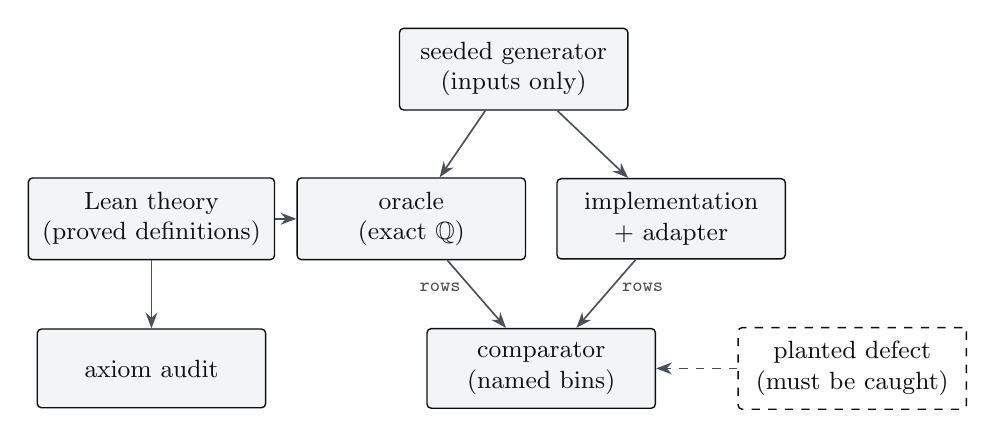
\begin{tikzpicture}[
  box/.style={draw=Ink, line width=0.5pt, fill=Surface, text=Ink, rounded corners=1.5pt,
    align=center, font=\small, inner sep=5pt, minimum height=10mm, minimum width=29mm},
  arr/.style={-{Stealth[length=2mm]}, line width=0.6pt, draw=InkMuted},
  lab/.style={font=\ttfamily\scriptsize, text=InkMuted}]
\node[box] (gen) at (4.6,1.9) {seeded generator\\(inputs only)};
\node[box] (theory) at (0,0) {Lean theory\\(proved definitions)};
\node[box] (oracle) at (3.3,0) {oracle\\(exact $\mathbb{Q}$)};
\node[box] (impl) at (6.6,0) {implementation\\+ adapter};
\node[box] (cmp) at (4.95,-1.9) {comparator\\(named bins)};
\node[box] (audit) at (0,-1.9) {axiom audit};
\node[box, dashed, fill=Background] (planted) at (8.9,-1.9) {planted defect\\(must be caught)};
\draw[arr] (gen) -- (oracle);
\draw[arr] (gen) -- (impl);
\draw[arr] (theory) -- (oracle);
\draw[arr] (theory) -- (audit);
\draw[arr] (oracle) -- node[left, lab, pos=0.4] {rows} (cmp);
\draw[arr] (impl) -- node[right, lab, pos=0.4] {rows} (cmp);
\draw[arr, dashed] (planted) -- (cmp);
\end{tikzpicture}
\caption{The measurement procedure. The generator never computes expected results;
those come only from the oracle.}
\label{fig:harness}
\end{figure}

The procedure follows \texttt{ledger-semantics} (\cref{fig:harness}). A seeded
generator writes case files containing inputs only. It favors the inputs where
implementations are known to have conventions: tied logits, words that are
themselves tokens, and merge tables with several splits of one string. A small
adapter per implementation runs the same cases and prints the oracle's row format.
The comparator places every case in exactly one named bin (agree, diverge, skipped
by either side, or missing), so nothing is dropped silently. Token rows are compared
as strings. Sampler rows require that a zero be matched by a zero and that nonzero
probabilities agree within $10^{-6}$, since llama.cpp stores logits in
\texttt{float32}. Each comparator is observed to fail: a planted defect, an adapter
that glues two tokens or one that inverts temperature, must be detected or the run
fails.

\paragraph{Tie divergences.} An implementation that keeps exactly $k$ tokens breaks
ties in its own order, which need not be the oracle's order by index. Every filter
treats tied tokens alike except for that choice, and tied tokens stay tied through
temperature and renormalization. Such an implementation must therefore agree with
the positional semantics up to a permutation of tied tokens. The harness checks
exactly this: the multiset of (logit, probability) pairs over the kept tokens must
equal that of the oracle's \texttt{q} rows. A divergence that fails this check is
reported as unexplained.

\begin{table}[t]
\centering\small
\caption{Measurements (\texttt{harness/run.sh 600}: four seeds of 600 cases each per
corpus). Lean 4.34.1, Mathlib v4.34.1, \texttt{tokenizers} 0.23.3, \texttt{tiktoken}
0.14.0, llama.cpp commit \texttt{a9d27ac} (2026-10-11).}
\label{tab:results}
\begin{tabularx}{\linewidth}{@{}>{\raggedright\arraybackslash}p{4.6cm}>{\raggedright\arraybackslash}X>{\raggedright\arraybackslash}X@{}}
\toprule
\qpth{Implementation} & \qpth{Compared against} & \qpth{Result}\\
\midrule
HF \texttt{tokenizers}, BPE, defaults & rule-rank BPE (\lean{bpe}) & 13{,}779 / 13{,}779 words identical\\
HF \texttt{tokenizers}, \lean{ignore_merges} & lookup, then rule-rank BPE & 13{,}779 / 13{,}779 identical\\
\texttt{tiktoken} & lookup, then concatenation-rank BPE & 13{,}779 / 13{,}779 identical\\
llama.cpp \lean{top_k}, \lean{top_p}, \lean{min_p}, \texttt{temp}, no ties & tie-keeping filters & 1{,}216 / 1{,}216 chains, $|\Delta p|\le5.1\times10^{-8}$\\
llama.cpp, with ties & tie-keeping, else positional & 939 + 245 / 1{,}184 chains; 0 unexplained\\
Planted defects (tokenizer, sampler) & --- & both detected\\
\bottomrule
\end{tabularx}
\end{table}

\Cref{tab:results} summarizes the results. Two findings came out of the
comparisons. First, \texttt{tiktoken} initially disagreed with the oracle's
concatenation-rank BPE on words that are themselves vocabulary tokens. The
disagreement was a convention, whole-word lookup. Following the
\texttt{ledger-semantics} rule that a divergence is either a defect in the
implementation or a convention the semantics has not yet recorded, we recorded it
as \lean{lookupFirst}, with its own theorems, after which agreement is exact.
Second, on the same random merge tables the two tokenizer libraries disagree with
each other on 439 of 13{,}779 words (3.2\%), and on 279 when Hugging Face uses
\lean{ignore_merges}. The oracle reproduces each library exactly, so every one of
these disagreements is predicted. \Cref{thm:bpeconv} states the condition under which
they cannot occur.

For sampling, llama.cpp agrees with the tie-keeping semantics on every tie-free
chain. On chains with ties, 245 of 1{,}184 diverge, and every one agrees with the
positional semantics up to a permutation of tied tokens. Some of these divergences
cascade: a tie cut by top-$k$ changes the renormalized masses that a later top-$p$
sees. A check that compared kept sets only after the fact would misclassify such
cases. Replaying the convention exactly classifies all of them.

% ===========================================================================
\section{Related work}

\paragraph{Formal methods for machine learning.} Most verification work on neural
networks proves properties of trained models, for example with SMT-based
methods~\cite{katz2017reluplex}. We verify the model-independent algorithms around
the model instead, and connect them to implementations through an oracle. The
denotational method follows Elliott~\cite{elliott2009denotational}. The use of a
proved semantics as a test oracle, the procedure of planted defects, and the
discipline of named skip bins follow \texttt{ledger-semantics}~\cite{ledgersemantics}.
Our category of finite stochastic maps is a special case of Fritz's Markov
categories~\cite{fritz2020markov}.

\paragraph{Tokenization.} Zouhar et al.\ give a formal analysis of BPE as an
optimization problem~\cite{zouhar2023bpe}. Gastaldi et al.\ treat tokenizers as
stochastic maps and study consistency of estimators~\cite{gastaldi2024foundations}.
Vieira et al.\ show how to turn token-level models into character-level
ones~\cite{vieira2024tokens}, which requires exactly the enumeration of
tokenizations we verify. Our no-compression theorem and the agreement criterion
between BPE conventions complement this work at the level of exact identities.

\paragraph{Decoding.} Top-$k$~\cite{fan2018hierarchical}, nucleus~\cite{holtzman2020curious}
and min-$p$~\cite{nguyen2025minp} sampling are usually specified by an algorithm over
sorted arrays, which leaves ties unspecified. \Cref{thm:topk} shows that this gap
cannot be closed by any symmetric rule. Speculative
sampling~\cite{leviathan2023speculative,chen2023speculative} is known to be lossless,
and its acceptance rate is the maximal-coupling bound~\cite{lindvall1992coupling}. Du et
al.\ characterize tightness measure-theoretically~\cite{du2023tight}. We give a
finite-depth statement and an explicit non-tight model.

\paragraph{Attention and inference systems.} Online softmax~\cite{milakov2018online}
underlies FlashAttention~\cite{dao2022flashattention} and its successors, and
KV caching is standard in serving systems~\cite{pope2023scaling,kwon2023vllm}. Our
contribution is the algebraic packaging, a commutative monoid with a free-monoid
homomorphism, and machine-checked proofs over arbitrary exponential characters.
Permutation equivariance of attention without positional encodings is
known~\cite{yun2020universal}.

\paragraph{Masked diffusion.} The time-independence of the optimal denoiser was
observed by Ou et al.~\cite{ou2025absorbing}, in the setting of
D3PM~\cite{austin2021d3pm}, MDLM~\cite{sahoo2024mdlm} and related
models~\cite{shi2024masked,nie2025llada}. We machine-check it, together with the
any-order chain rule and the inexactness of parallel unmasking.

% ===========================================================================
\section{Limitations}

Analysis on the reals enters only through exponential characters, and there is no
measure theory, so sampling and tightness are stated through finite quantities. The
oracle's temperature is restricted to $1/n$, which keeps softmax rational. The
theorems hold for every temperature, but the oracle cannot evaluate an irrational
softmax. Speculative decoding is proved for one drafted token. The sequence version
follows by induction and is not yet formalized. Nothing is proved about
floating-point arithmetic: implementations are compared with exact values within a
stated tolerance. A decision that lies exactly on a floating-point boundary could in
principle diverge, and none occurred in our runs. The diffusion theory covers
absorbing diffusion, not Gaussian diffusion. The chat protocol models tool calling in
its common request-and-result form, not any vendor's specification. The measurements
cover tokenizers and samplers; attention kernels, speculative decoders, chat
renderers and diffusion samplers are evaluated by the oracle but not yet compared
against implementations.

% ===========================================================================
\section{Conclusion}

The inference side of LLMs is small enough to be given a precise meaning and large
enough that its implementations disagree. A machine-checked semantics separates
what is meaning from what is convention. It proves which reorderings, cachings and
tilings are harmless, and it shows that some properties folklore expects, such as
symmetric exact top-$k$, compositional compressing tokenizers and unambiguous plain-text
templates, cannot exist. Connected to an exact oracle, the same definitions become
a test instrument. Every divergence it surfaces is either a defect in an
implementation or a convention that belongs in the semantics.

\paragraph{Availability.} The Lean development, oracle, harness, and recorded
measurement log accompany this paper.

\paragraph{Acknowledgments.} The structure of this work follows
\texttt{ledger-semantics} by John Wiegley. The formalization and harness were
developed with the assistance of an AI system (Claude, Anthropic).

% ===========================================================================
\begin{thebibliography}{99}\small

\bibitem{austin2021d3pm}
J.~Austin, D.~D. Johnson, J.~Ho, D.~Tarlow, and R.~van~den Berg.
\newblock Structured denoising diffusion models in discrete state-spaces.
\newblock In \emph{NeurIPS}, 2021.

\bibitem{chen2023speculative}
C.~Chen, S.~Borgeaud, G.~Irving, J.-B. Lespiau, L.~Sifre, and J.~Jumper.
\newblock Accelerating large language model decoding with speculative sampling.
\newblock arXiv:2302.01318, 2023.

\bibitem{dao2022flashattention}
T.~Dao, D.~Y. Fu, S.~Ermon, A.~Rudra, and C.~R{\'e}.
\newblock {FlashAttention}: Fast and memory-efficient exact attention with {IO}-awareness.
\newblock In \emph{NeurIPS}, 2022.

\bibitem{demoura2021lean4}
L.~de~Moura and S.~Ullrich.
\newblock The {Lean} 4 theorem prover and programming language.
\newblock In \emph{CADE-28}, 2021.

\bibitem{du2023tight}
L.~Du, L.~Torroba~Hennigen, T.~Pimentel, C.~Meister, J.~Eisner, and R.~Cotterell.
\newblock A measure-theoretic characterization of tight language models.
\newblock In \emph{ACL}, 2023.

\bibitem{elliott2009denotational}
C.~Elliott.
\newblock Denotational design with type class morphisms.
\newblock Technical Report 2009-01, LambdaPix, 2009.

\bibitem{fan2018hierarchical}
A.~Fan, M.~Lewis, and Y.~Dauphin.
\newblock Hierarchical neural story generation.
\newblock In \emph{ACL}, 2018.

\bibitem{fritz2020markov}
T.~Fritz.
\newblock A synthetic approach to {Markov} kernels, conditional independence and theorems on sufficient statistics.
\newblock \emph{Advances in Mathematics}, 370, 2020.

\bibitem{gastaldi2024foundations}
J.~L. Gastaldi, J.~Terilla, L.~Malagutti, B.~DuSell, T.~Vieira, and R.~Cotterell.
\newblock The foundations of tokenization: Statistical and computational concerns.
\newblock arXiv:2407.11606, 2024.

\bibitem{greshake2023injection}
K.~Greshake, S.~Abdelnabi, S.~Mishra, C.~Endres, T.~Holz, and M.~Fritz.
\newblock Not what you've signed up for: Compromising real-world {LLM}-integrated applications with indirect prompt injection.
\newblock In \emph{AISec}, 2023.

\bibitem{holtzman2020curious}
A.~Holtzman, J.~Buys, L.~Du, M.~Forbes, and Y.~Choi.
\newblock The curious case of neural text degeneration.
\newblock In \emph{ICLR}, 2020.

\bibitem{katz2017reluplex}
G.~Katz, C.~Barrett, D.~L. Dill, K.~Julian, and M.~J. Kochenderfer.
\newblock Reluplex: An efficient {SMT} solver for verifying deep neural networks.
\newblock In \emph{CAV}, 2017.

\bibitem{kwon2023vllm}
W.~Kwon, Z.~Li, S.~Zhuang, Y.~Sheng, L.~Zheng, C.~H. Yu, J.~E. Gonzalez, H.~Zhang, and I.~Stoica.
\newblock Efficient memory management for large language model serving with {PagedAttention}.
\newblock In \emph{SOSP}, 2023.

\bibitem{ledgersemantics}
J.~Wiegley.
\newblock ledger-semantics: Mathematical semantics of {Ledger}, the double-entry accounting tool.
\newblock \url{https://github.com/ledger/ledger-semantics}, 2026.

\bibitem{leviathan2023speculative}
Y.~Leviathan, M.~Kalman, and Y.~Matias.
\newblock Fast inference from transformers via speculative decoding.
\newblock In \emph{ICML}, 2023.

\bibitem{lindvall1992coupling}
T.~Lindvall.
\newblock \emph{Lectures on the Coupling Method}.
\newblock Wiley, 1992.

\bibitem{liu2023ring}
H.~Liu, M.~Zaharia, and P.~Abbeel.
\newblock Ring attention with blockwise transformers for near-infinite context.
\newblock arXiv:2310.01889, 2023.

\bibitem{mathlib2020}
The mathlib Community.
\newblock The {Lean} mathematical library.
\newblock In \emph{CPP}, 2020.

\bibitem{milakov2018online}
M.~Milakov and N.~Gimelshein.
\newblock Online normalizer calculation for softmax.
\newblock arXiv:1805.02867, 2018.

\bibitem{nguyen2025minp}
M.~N. Nguyen, A.~Baker, C.~Neo, A.~Roush, A.~Kirsch, and R.~Shwartz-Ziv.
\newblock Turning up the heat: Min-p sampling for creative and coherent {LLM} outputs.
\newblock In \emph{ICLR}, 2025.

\bibitem{nie2025llada}
S.~Nie, F.~Zhu, Z.~You, X.~Zhang, J.~Ou, J.~Hu, J.~Zhou, Y.~Lin, J.-R. Wen, and C.~Li.
\newblock Large language diffusion models.
\newblock arXiv:2502.09992, 2025.

\bibitem{ou2025absorbing}
J.~Ou, S.~Nie, K.~Xue, F.~Zhu, J.~Sun, Z.~Li, and C.~Li.
\newblock Your absorbing discrete diffusion secretly models the conditional distributions of clean data.
\newblock In \emph{ICLR}, 2025.

\bibitem{pope2023scaling}
R.~Pope, S.~Douglas, A.~Chowdhery, J.~Devlin, J.~Bradbury, J.~Heek, K.~Xiao, S.~Agrawal, and J.~Dean.
\newblock Efficiently scaling transformer inference.
\newblock In \emph{MLSys}, 2023.

\bibitem{rabe2021selfattention}
M.~N. Rabe and C.~Staats.
\newblock Self-attention does not need {$O(n^2)$} memory.
\newblock arXiv:2112.05682, 2021.

\bibitem{radford2019gpt2}
A.~Radford, J.~Wu, R.~Child, D.~Luan, D.~Amodei, and I.~Sutskever.
\newblock Language models are unsupervised multitask learners.
\newblock OpenAI technical report, 2019.

\bibitem{sahoo2024mdlm}
S.~S. Sahoo, M.~Arriola, Y.~Schiff, A.~Gokaslan, E.~Marroquin, J.~T. Chiu, A.~Rush, and V.~Kuleshov.
\newblock Simple and effective masked diffusion language models.
\newblock In \emph{NeurIPS}, 2024.

\bibitem{sennrich2016bpe}
R.~Sennrich, B.~Haddow, and A.~Birch.
\newblock Neural machine translation of rare words with subword units.
\newblock In \emph{ACL}, 2016.

\bibitem{shi2024masked}
J.~Shi, K.~Han, Z.~Wang, A.~Doucet, and M.~K. Titsias.
\newblock Simplified and generalized masked diffusion for discrete data.
\newblock In \emph{NeurIPS}, 2024.

\bibitem{vieira2024tokens}
T.~Vieira, B.~LeBrun, M.~Giulianelli, J.~L. Gastaldi, B.~DuSell, J.~Terilla, T.~J. O'Donnell, and R.~Cotterell.
\newblock From language models over tokens to language models over characters.
\newblock arXiv:2412.03719, 2024.

\bibitem{wolf2020transformers}
T.~Wolf et~al.
\newblock Transformers: State-of-the-art natural language processing.
\newblock In \emph{EMNLP: System Demonstrations}, 2020.

\bibitem{xiao2024sinks}
G.~Xiao, Y.~Tian, B.~Chen, S.~Han, and M.~Lewis.
\newblock Efficient streaming language models with attention sinks.
\newblock In \emph{ICLR}, 2024.

\bibitem{yun2020universal}
C.~Yun, S.~Bhojanapalli, A.~S. Rawat, S.~J. Reddi, and S.~Kumar.
\newblock Are transformers universal approximators of sequence-to-sequence functions?
\newblock In \emph{ICLR}, 2020.

\bibitem{zouhar2023bpe}
V.~Zouhar, C.~Meister, J.~L. Gastaldi, L.~Du, T.~Vieira, M.~Sachan, and R.~Cotterell.
\newblock A formal perspective on byte-pair encoding.
\newblock In \emph{Findings of ACL}, 2023.

\end{thebibliography}

\end{document}
"
% ---------------------------------------------------------------------------
\documentclass[10pt]{article}

\newif\ifqptdark
\qptdarkfalse   % print edition (light). \qptdarktrue gives the dark screen edition.
\ifdefined\qptdarkedition\qptdarktrue\fi  % or: xelatex "\def\qptdarkedition{}% !TeX program = xelatex
% ---------------------------------------------------------------------------
%  A Machine-Checked Semantics of LLM Inference
%  Daniel Arango Sohm, Universidad EAFIT
%
%  Typeset in the QPT visual design system:
%    * neutral-first: Ink on Background carries the document;
%    * paradigm colours are semantic only. This paper belongs to none of the
%      five paradigms, so no paradigm colour appears in its content; the
%      colours appear only in the QPT mark itself;
%    * no gradients;
%    * Space Grotesk for display, Inter for body text, IBM Plex Mono for
%      technical, numeric, label, code and proof-oriented content.
%
%  Compile with:  xelatex llm-semantics-qpt.tex   (twice, for references)
%  Dark screen edition: set \qptdarktrue below, or run
%    xelatex -jobname=llm-semantics-qpt-dark "\def\qptdarkedition{}\input{llm-semantics-qpt}"
% ---------------------------------------------------------------------------
\documentclass[10pt]{article}

\newif\ifqptdark
\qptdarkfalse   % print edition (light). \qptdarktrue gives the dark screen edition.
\ifdefined\qptdarkedition\qptdarktrue\fi  % or: xelatex "\def\qptdarkedition{}\input{llm-semantics-qpt}"

\usepackage[a4paper,textwidth=15.4cm,textheight=23.6cm,top=3.0cm,headsep=0.9cm,footskip=1.2cm]{geometry}
\usepackage{amsmath,amssymb,amsthm,mathtools}
\usepackage{fontspec}
\usepackage{booktabs,tabularx,array}
\usepackage[protrusion=true,expansion=false]{microtype}
\usepackage[table]{xcolor}
\usepackage{graphicx}
\usepackage{fvextra}
\usepackage{enumitem}
\usepackage{caption}
\usepackage{titlesec}
\usepackage{fancyhdr}
\usepackage[most]{tcolorbox}
\usepackage{tikz}
\usetikzlibrary{arrows.meta}
\usepackage{hyperref}
\usepackage[nameinlink,capitalise]{cleveref}

% ---------------------------------------------------------------------------
%  Colour tokens
% ---------------------------------------------------------------------------
% Neutral foundation. Ink and Background invert between the two editions.
\ifqptdark
  \definecolor{Background}{HTML}{0B0C0E}
  \definecolor{Surface}{HTML}{16181B}
  \definecolor{Border}{HTML}{2B2E33}
  \definecolor{Ink}{HTML}{EDEEF0}
  \definecolor{InkMuted}{HTML}{A9AEB6}
  \definecolor{InkFaint}{HTML}{5A5F67}   % decoration only, never meaningful text
\else
  \definecolor{Background}{HTML}{FFFFFF}
  \definecolor{Surface}{HTML}{F3F4F5}
  \definecolor{Border}{HTML}{DADDE1}
  \definecolor{Ink}{HTML}{0E0F11}
  \definecolor{InkMuted}{HTML}{4B4F57}
  \definecolor{InkFaint}{HTML}{A3A7AE}   % decoration only, never meaningful text
\fi
% Paradigm colours: fixed in both editions, semantic only.
\definecolor{Quantum}{HTML}{5BAD1E}
\definecolor{Photonic}{HTML}{F0AB00}
\definecolor{Thermodynamic}{HTML}{E8690A}
\definecolor{Ternary}{HTML}{8A8A8A}
\definecolor{Bio}{HTML}{1AAB7C}

\ifqptdark\pagecolor{Background}\fi

% ---------------------------------------------------------------------------
%  Typography
% ---------------------------------------------------------------------------
\setmainfont{Inter}[
  Path=fonts/, Extension=.otf, Scale=0.94,
  UprightFont=*-Regular, ItalicFont=*-Italic,
  BoldFont=*-SemiBold, BoldItalicFont=*-SemiBoldItalic]
\setmonofont{IBMPlexMono}[
  Path=fonts/, Extension=.ttf, Scale=MatchLowercase,
  UprightFont=*-Regular, ItalicFont=*-Italic, BoldFont=*-SemiBold]
\newfontfamily\qptdisplay{SpaceGrotesk}[
  Path=fonts/, Extension=.otf, UprightFont=*-Medium, BoldFont=*-Bold]
\newfontfamily\qptdisplaylight{SpaceGrotesk}[
  Path=fonts/, Extension=.otf, UprightFont=*-Regular]
\newfontfamily\qptlabelfont{IBMPlexMono}[
  Path=fonts/, Extension=.ttf, Scale=MatchLowercase, UprightFont=*-Medium,
  LetterSpace=6]
\setsansfont{Inter}[
  Path=fonts/, Extension=.otf, Scale=0.94,
  UprightFont=*-Regular, ItalicFont=*-Italic,
  BoldFont=*-SemiBold, BoldItalicFont=*-SemiBoldItalic]
\linespread{1.16}
\setlength{\emergencystretch}{2.5em}
\AtBeginDocument{\raggedright\setlength{\parindent}{0pt}}
\setlength{\parindent}{0pt}
\setlength{\parskip}{0.55em}

% A label: IBM Plex Mono, upper case, tracked.
\newcommand{\qptlabel}[1]{{\qptlabelfont\footnotesize\MakeUppercase{#1}}}
% Technical names (Lean declarations, files) in IBM Plex Mono.
\newcommand{\lean}[1]{\texttt{\detokenize{#1}}}
\newcommand{\leanref}[1]{\par\smallskip\noindent
  {\ttfamily\footnotesize\upshape\raggedright\color{InkMuted}LEAN\enspace #1\par}}

% Ink is the normal colour everywhere, including floats, heads and footnotes.
\makeatletter
\AtBeginDocument{\color{Ink}\global\let\default@color\current@color}
\makeatother

% ---------------------------------------------------------------------------
%  Mathematical notation
% ---------------------------------------------------------------------------
\newcommand{\K}{\Bbbk}
\newcommand{\Dist}{\mathrm{Dist}}
\newcommand{\restr}[2]{#1|_{#2}}
\newcommand{\topk}{\mathrm{TopK}}
\newcommand{\topp}{\mathrm{TopP}}
\newcommand{\minp}{\mathrm{MinP}}
\newcommand{\sharpen}{\mathrm{sharpen}}
\newcommand{\abv}{\mathrm{above}}
\newcommand{\tv}{\mathrm{tv}}
\newcommand{\dec}{\mathrm{dec}}
\newcommand{\enc}{\mathrm{enc}}
\newcommand{\softmax}{\mathrm{softmax}}
\newcommand{\attend}{\mathrm{attend}}
\newcommand{\Iv}[1]{[\![#1]\!]}
\newcommand{\Mask}{\bot}

% ---------------------------------------------------------------------------
%  Headings: section numbers as labels, titles in Space Grotesk
% ---------------------------------------------------------------------------
\makeatletter
\newcommand{\qptsecnum}[1]{{\qptlabelfont\small\color{InkMuted}\two@digits{#1}}}
\makeatother
\titleformat{\section}
  {\qptdisplay\fontsize{14.5}{18}\selectfont\color{Ink}}
  {\qptsecnum{\value{section}}}{0.9em}{}
\titleformat{name=\section,numberless}
  {\qptdisplay\fontsize{14.5}{18}\selectfont\color{Ink}}{}{0pt}{}
\titlespacing*{\section}{0pt}{1.9em}{0.7em}
\titleformat{\paragraph}[runin]
  {\qptdisplay\normalsize\color{Ink}}{}{0pt}{}
\titlespacing*{\paragraph}{0pt}{0.9em}{0.6em}

% ---------------------------------------------------------------------------
%  Statements
% ---------------------------------------------------------------------------
\newtheoremstyle{qpt}
  {0.9em}{0.9em}
  {\normalfont}{}
  {\qptlabelfont\footnotesize}{}
  {\newline}
  {\MakeUppercase{\thmname{#1}\thmnumber{~#2}}%
   \thmnote{\enspace{\qptdisplay\normalsize\color{Ink}#3}}}
\theoremstyle{qpt}
\newtheorem{theorem}{Theorem}
\newtheorem{proposition}[theorem]{Proposition}
\newtheorem{corollary}[theorem]{Corollary}
\newtheorem{lemma}[theorem]{Lemma}
\newtheorem{definition}[theorem]{Definition}
\newtheorem{remark}[theorem]{Remark}

% Proofs: a tracked label and a neutral end mark.
\makeatletter
\renewcommand{\qedsymbol}{{\color{InkMuted}\rule{0.5em}{0.5em}}}
\renewenvironment{proof}[1][Proof]{\par\pushQED{\qed}\normalfont\topsep0.5em\relax
  \trivlist\item[\hskip\labelsep\qptlabel{#1}\hspace{0.6em}]\ignorespaces}
  {\popQED\endtrivlist\@endpefalse}
\makeatother

% ---------------------------------------------------------------------------
%  Code: IBM Plex Mono on a neutral surface, with a hairline on the left
% ---------------------------------------------------------------------------
\tcbset{colupper=Ink, collower=Ink}
\tcbset{qptcode/.style={enhanced, colback=Surface, colframe=Surface,
  boxrule=0pt, arc=0pt, left=9pt, right=8pt, top=5pt, bottom=5pt,
  borderline west={1.2pt}{0pt}{InkFaint}, before skip=0.7em, after skip=0.7em}}
\newenvironment{leancode}
  {\VerbatimEnvironment\begin{tcolorbox}[qptcode]%
   \begin{Verbatim}[fontsize=\small,commandchars=\\\{\},
     codes={\catcode`\$=3\catcode`\^=7},formatcom=\color{Ink}]}
  {\end{Verbatim}\end{tcolorbox}}
\newenvironment{casecode}
  {\VerbatimEnvironment\begin{tcolorbox}[qptcode,before skip=0pt,after skip=0pt]%
   \begin{Verbatim}[fontsize=\footnotesize,formatcom=\color{Ink}]}
  {\end{Verbatim}\end{tcolorbox}}

% ---------------------------------------------------------------------------
%  Floats, tables, captions
% ---------------------------------------------------------------------------
\DeclareCaptionLabelFormat{qpt}{\qptlabel{#1~#2}}
\DeclareCaptionLabelSeparator{qptsep}{\quad}
\captionsetup{labelformat=qpt, labelsep=qptsep, font={small,color=Ink},
  justification=raggedright, singlelinecheck=false, skip=6pt}
\newcommand{\qpth}[1]{\qptlabel{#1}}
\arrayrulecolor{Ink}
\setlength{\heavyrulewidth}{0.7pt}
\setlength{\lightrulewidth}{0.35pt}
\renewcommand{\arraystretch}{1.22}

% ---------------------------------------------------------------------------
%  Running heads
% ---------------------------------------------------------------------------
\pagestyle{fancy}
\fancyhf{}
\fancyhead[L]{{\color{Ink}\qptlabel{Machine-checked semantics of LLM inference}}}
\fancyhead[R]{{\color{Ink}\qptlabel{D. Arango Sohm}}}
\fancyfoot[R]{{\ttfamily\small\color{InkMuted}\thepage}}
\renewcommand{\headrule}{{\color{Border}\hrule height 0.4pt}\vspace{-0.4pt}}
\renewcommand{\headrulewidth}{0.4pt}
\fancypagestyle{qptfirst}{\fancyhf{}%
  \fancyfoot[R]{{\ttfamily\small\color{InkMuted}\thepage}}%
  \renewcommand{\headrulewidth}{0pt}\renewcommand{\headrule}{}}

% ---------------------------------------------------------------------------
%  Links and references: neutral, never accent-coloured text
% ---------------------------------------------------------------------------
\hypersetup{colorlinks=true, linkcolor=Ink, citecolor=Ink, urlcolor=Ink,
  pdftitle={A Machine-Checked Semantics of LLM Inference},
  pdfauthor={Daniel Arango Sohm},
  pdfsubject={Formal semantics of large language model inference in Lean 4},
  pdfkeywords={Lean 4, Mathlib, formal verification, LLM inference, sampling,
    tokenization, attention, speculative decoding, diffusion language models}}
\makeatletter
\renewcommand{\@biblabel}[1]{{\ttfamily\color{InkMuted}[#1]}}
\renewcommand{\@cite}[2]{{\ttfamily[#1\if@tempswa, #2\fi]}}
\makeatother
\renewcommand{\refname}{References}

\setlist{itemsep=2pt, topsep=4pt}
\setlist[itemize]{label={\color{InkMuted}\textbullet}}

\begin{document}
\thispagestyle{qptfirst}

% ----------------------------------------------------------------- masthead
\noindent
\begin{minipage}[c]{0.5\linewidth}
  \includegraphics[height=1.9cm]{qpt-logo.png}
\end{minipage}%
\begin{minipage}[c]{0.5\linewidth}\raggedleft
  \qptlabel{Preprint}\\[2pt]
  \qptlabel{October 2026}
\end{minipage}

\vspace{1.6em}
{\color{Border}\rule{\linewidth}{0.4pt}}
\vspace{1.1em}

{\qptdisplay\fontsize{25}{29.5}\selectfont\color{Ink}
A Machine-Checked Semantics\\ of LLM Inference\par}
\vspace{0.55em}
{\qptdisplaylight\fontsize{13}{17}\selectfont\color{InkMuted}
Sampling, Attention, Tokenization, Chat, Decoding,\\ and Diffusion in Lean~4\par}

\vspace{1.5em}
{\large\bfseries Daniel Arango Sohm}\par
\vspace{0.15em}
{\color{InkMuted}Universidad EAFIT, Medellín, Colombia\\
Former member of the QPT team}\par

\vspace{1.4em}
% ----------------------------------------------------------------- abstract
\begin{tcolorbox}[enhanced, colback=Surface, colframe=Surface, colupper=Ink, boxrule=0pt,
  arc=0pt, left=12pt, right=12pt, top=9pt, bottom=10pt]
\qptlabel{Abstract}\par\vspace{0.35em}
{\small
The inference side of a large language model is a stack of small algorithms:
tokenizers, attention kernels, key--value caches, sampling filters, speculative
decoders, chat templates, and diffusion samplers. Each has several independent
implementations, and those implementations are usually tested against one another
rather than against a definition. We give these components a single mathematical
semantics, formalized in Lean~4 against Mathlib. The development comprises about
4{,}600 lines and 270 named theorems, and every declaration depends only on Lean's
three standard axioms. It proves the exact algebra of sampling filters, the
losslessness and optimality of speculative sampling, and the correctness of
key--value caching and of FlashAttention-style online softmax as a commutative
monoid. It proves that byte-pair encoding is lossless under every merge priority,
together with a decidable criterion for when the Hugging Face and \texttt{tiktoken}
conventions agree, a protocol checker for tool calls, and the time-independence of
the masked-diffusion denoiser. It also proves six negative results. No sampling
rule that treats tokens symmetrically can always keep exactly $k$ tokens. No
tokenizer that compresses can respect concatenation. Every chat template that writes
its role markers in the content alphabet is ambiguous. No transformer without
positional information can copy a fixed position. An autoregressive model need not
define a distribution over strings. Parallel unmasking in diffusion is inexact.
From the same definitions we build an executable oracle that evaluates test cases in
exact rational arithmetic, and a harness that measures implementations against it.
On 2{,}400 random merge tables, Hugging Face \texttt{tokenizers} and
\texttt{tiktoken} each agree with the oracle on all 13{,}779 test words, while
disagreeing with each other on 3.2\% of them. On 2{,}400 random sampler chains,
every divergence of llama.cpp from the tie-keeping semantics is accounted for
exactly by the positional semantics that the impossibility theorem forces.
\par}
\end{tcolorbox}

\vspace{0.3em}
\noindent\qptlabel{Keywords}\enspace{\small Lean~4 · Mathlib · formal verification ·
LLM inference · sampling · tokenization · attention · speculative decoding ·
diffusion language models}

\vspace{0.4em}
{\color{Border}\rule{\linewidth}{0.4pt}}

% ===========================================================================
\section{Introduction}

A deployed language model is a function from parameters and a context to a
distribution over tokens. Turning that distribution into text requires more
machinery. A tokenizer maps strings to token sequences. Attention kernels compute
the model's reads over a cached context. A chain of sampling filters reshapes the
next-token distribution. A speculative decoder may verify drafted tokens, a chat
template linearizes a conversation, and a diffusion sampler may unmask several
positions at once. Each of these components exists in many implementations, such as
Hugging Face \texttt{transformers} and \texttt{tokenizers}~\cite{wolf2020transformers},
\texttt{tiktoken}, vLLM~\cite{kwon2023vllm}, and llama.cpp. Their tests mostly
compare one implementation with another, or with remembered behavior.

This paper follows a different discipline, \emph{denotational design}~\cite{elliott2009denotational}.
One first says precisely what a thing means, then requires every operation to
preserve that meaning, and lets the implementation be whatever the equations force
it to be. The approach is that of \texttt{ledger-semantics}~\cite{ledgersemantics},
which formalizes double-entry accounting in Lean and uses the result as a test oracle
for the C++ Ledger program. We apply it to LLM inference. A sampling filter means
conditioning a distribution on a set. A KV-cached decoder means causal attention over
the whole prefix. A FlashAttention kernel means a softmax-weighted average. A chat
template means an injective encoding of a transcript. The theorems state when an
implementation preserves that meaning, and several of them state that no
implementation can.

\paragraph{Contributions.}
\begin{itemize}[leftmargin=*,itemsep=2pt]
\item A Lean~4 formalization against Mathlib~\cite{mathlib2020,demoura2021lean4}
  of sampling, speculative decoding, softmax and attention, tokenization, chat
  transcripts, autoregressive decoding, and masked diffusion
  (\cref{sec:foundations,sec:sampling,sec:spec,sec:attention,sec:tokenization,sec:chat,sec:decoding,sec:diffusion}).
  All definitions are stated over an arbitrary linearly ordered field, so one proof
  covers the real numbers of the literature and the exact rationals of the oracle.
\item Positive results in a common framework. They include the algebra of
  sampling filters, the optimality of speculative sampling, an online-softmax
  commutative monoid, a generic correctness theorem for BPE with a decidable
  agreement criterion between the two conventions in use, a protocol checker for
  tool calls, and the any-order chain rule for masked diffusion.
\item Six negative results that explain design constraints visible across
  implementations (\cref{sec:negative}).
\item An executable oracle that evaluates case files under the proved
  definitions in exact arithmetic, and a measurement of Hugging Face
  \texttt{tokenizers}, \texttt{tiktoken}, and llama.cpp against it (\cref{sec:oracle,sec:measure}).
\end{itemize}

Several of the positive results are known: losslessness of speculative
sampling~\cite{leviathan2023speculative,chen2023speculative}, correctness of online
softmax~\cite{milakov2018online,dao2022flashattention}, time-independence of the
absorbing-diffusion posterior~\cite{ou2025absorbing}, and the role of permutation
equivariance~\cite{yun2020universal}. Our contribution for these is a machine-checked
statement in one framework, connected to an oracle. To our knowledge the
following are not stated elsewhere in the form given here: the impossibility of
symmetric exact top-$k$ and nucleus selection, the no-compression theorem for
homomorphic tokenizers, the ambiguity of every in-band chat template, and the
decidable agreement criterion between merge-rule and concatenation-rank BPE.

% ===========================================================================
\section{Method and trust base}\label{sec:method}

The development is a Lean~4 library (Lean 4.34.1, Mathlib v4.34.1) of eleven
theory modules and two executable modules (\cref{tab:modules}). It is built with
warnings promoted to errors, so an unproved theorem (\lean{sorry}) fails the build.
A separate audit program walks every declaration in the library, 853 in all, and
fails unless each depends only on propositional extensionality, the axiom of choice,
and quotient soundness. The audit has been observed to fail: a planted proof by
\lean{native_decide}, which introduces an auxiliary axiom trusting compiled code, is
rejected. The warnings-as-errors build alone does not catch it. Concrete
counterexamples are therefore proved by \lean{decide}, whose certificate the kernel
checks by evaluation.

\begin{table}[t]
\centering\small
\caption{Modules of the development. Lines and named theorems and lemmas per module.}
\label{tab:modules}
\begin{tabularx}{\linewidth}{@{}l>{\raggedright\arraybackslash}X>{\ttfamily}r>{\ttfamily}r@{}}
\toprule
\qpth{Module} & \qpth{Content} & \qpth{Lines} & \qpth{Thms} \\
\midrule
\lean{Dist} & finite distributions, conditioning, total variation, $\mathsf{FinStoch}$ & 383 & 34\\
\lean{Sampling} & top-$k$, top-$p$, min-$p$, temperature, ties, inverse CDF & 732 & 46\\
\lean{Counterexamples} & kernel-checked failures of sampler laws & 52 & 4\\
\lean{Speculative} & speculative sampling, couplings & 194 & 17\\
\lean{Softmax} & exponential characters, masking, temperature & 220 & 23\\
\lean{Attention} & equivariance, causality, KV cache, online softmax & 573 & 38\\
\lean{Real} & $\exp$ as a character; textbook restatements & 51 & 4\\
\lean{Tokenization} & free-monoid decoding, BPE conventions, enumeration & 860 & 49\\
\lean{Chat} & tool-call protocol, rendering & 440 & 21\\
\lean{Decoding} & mass conservation, tightness, greedy decoding & 245 & 15\\
\lean{Diffusion} & masked diffusion, posterior, chain rule & 379 & 18\\
\lean{Oracle}, \lean{Driver} & case parsing and exact evaluation & 465 & 1\\
\midrule
Total & & 4{,}594 & 270\\
\bottomrule
\end{tabularx}
\end{table}

\paragraph{Numbers.} Every probability lives in an arbitrary field $\K$ with a
compatible linear order (\lean{[Field K] [LinearOrder K] [IsStrictOrderedRing K]}).
The oracle instantiates $\K=\mathbb{Q}$, so its arithmetic is exact. The analytic
statements instantiate $\K=\mathbb{R}$. No measure theory is used. Sampling is made
precise through interval statements (\cref{thm:invcdf}), and tightness through
masses at finite depth (\cref{sec:decoding}).

% ===========================================================================
\section{Foundations}\label{sec:foundations}

\begin{definition}[Finite distribution]
For a finite type $\alpha$, $\Dist_\K(\alpha)$ is the type of functions
$p:\alpha\to\K$ with $p(a)\ge 0$ for all $a$ and $\sum_a p(a)=1$.
\leanref{\lean{Dist}}
\end{definition}

\begin{leancode}
structure Dist ($\K$ : Type u) [Field $\K$] [LinearOrder $\K$] [IsStrictOrderedRing $\K$]
    ($\alpha$ : Type v) [Fintype $\alpha$] where
  prob : $\alpha$ $\to$ $\K$
  nonneg : $\forall$ a, 0 $\le$ prob a
  sum_eq_one : $\sum$ a, prob a = 1
\end{leancode}

The single operation through which masks, filters and grammar constraints act is
conditioning. For $S\subseteq\alpha$ with $p(S)>0$, write
$\restr{p}{S}(a)=\Iv{a\in S}\,p(a)/p(S)$ (\lean{Dist.restrict}).

\begin{lemma}[Conditioning]\label{lem:restrict}
$\restr{(\restr{p}{S})}{T}=\restr{p}{S\cap T}$ whenever the masses involved are
positive. Moreover $\restr{p}{S}=\restr{p}{S'}$ whenever $S$ and $S'$ contain the same
outcomes of positive probability.
\leanref{\lean{restrict_restrict}, \lean{restrict_congr}}
\end{lemma}

The finite distribution monad (point masses and \lean{bind}) satisfies the monad
laws. Finite types and stochastic maps $\alpha\to\Dist_\K(\beta)$ form a category
$\mathsf{FinStoch}_\K$, given as an instance of Mathlib's \lean{Category} whose
composition is Kleisli composition (\lean{FinStoch.category}). Total variation is
$\tv(p,q)=\sum_a\max(0,p(a)-q(a))$. We prove
$\tv(p,q)=\tfrac12\sum_a|p(a)-q(a)|$, $\sum_a\min(p(a),q(a))=1-\tv(p,q)$, and
$\tv(p,q)=0\iff p=q$.

% ===========================================================================
\section{Sampling}\label{sec:sampling}

Let $V$ be a finite vocabulary and $p:V\to\K$. Write
$\abv_p(v)=\{u: p(v)<p(u)\}$ for the tokens strictly preferred to $v$. The three
standard filters keep the sets
\begin{gather*}
\topk_k(p)=\{v: |\abv_p(v)|<k\},\qquad
\minp_m(p)=\{v:\forall u,\; m\,p(u)\le p(v)\},\\
\topp_P(p)=\Bigl\{v: \textstyle\sum_{u\in\abv_p(v)}p(u)<P\Bigr\},
\end{gather*}
and the filtered distribution is the conditioning $\restr{p}{S}$ on the kept set
$S$. For distinct probabilities, $\topp_P$ is the usual rule ``sort in descending
order and keep the shortest prefix whose mass reaches $P$''. With ties, all three
keep every tied token. Temperature $1/n$ is
$\sharpen_n(p)(v)=p(v)^n/\sum_u p(u)^n$, which stays inside $\mathbb{Q}$. In
\cref{sec:attention} we show that it equals $\softmax(n\cdot z)$ when
$p=\softmax(z)$. Every kept set contains a most probable token, provided $k\ge1$,
$P>0$ and $m\le1$, so no filter can produce an empty distribution.

\begin{theorem}[Sampler algebra]\label{thm:algebra}
For $k,k'\ge1$, $m,m'\le1$ and $n\ge1$, and writing filters in the order they are
applied,
\begin{enumerate}[label=(\roman*),itemsep=1pt]
\item top-$k$ then top-$k'$ equals top-$\min(k,k')$;
\item min-$m$ then min-$m'$ equals min-$\max(m,m')$; in particular both filters are idempotent;
\item top-$k$ and min-$m$ commute;
\item top-$k$ and temperature $1/n$ commute.
\end{enumerate}
\leanref{\lean{topK_topK}, \lean{minP_minP}, \lean{topK_minP_comm}, \lean{topK_sharpen_comm}}
\end{theorem}

\begin{proof}[Proof sketch]
All three kept sets are \emph{upward closed}: if $v$ is kept and $p(v)<p(u)$, then
$u$ is kept. Conditioning on an upward-closed set $S$ leaves $\abv(v)$ unchanged for
$v\in S$ (\lean{above_restrict}), and min-$p$ is insensitive to conditioning on a set
that contains a maximizer (\lean{minP_restrict_iff}). Each identity then reduces,
through \cref{lem:restrict}, to an equality of kept sets. For (iv), $x\mapsto x^n$
is strictly increasing on $[0,\infty)$, and top-$k$ depends only on the order of the
scores (\lean{topKSet_congr}).
\end{proof}

The laws one might expect beyond \cref{thm:algebra} are false. With
$p_0=(\tfrac12,\tfrac3{10},\tfrac15)$, the kernel evaluates the following
(\lean{Counterexamples}).

\begin{proposition}[Failed laws]\label{prop:counter}
\leavevmode\vspace{-0.5\baselineskip}
\begin{enumerate}[label=(\roman*),itemsep=1pt]
\item Top-$p$ is not idempotent: one pass of $\topp_{3/5}$ gives token~1 the probability $\tfrac38$, and a second pass gives it~$0$.
\item Top-$p$ does not commute with top-$k$: top-$p$ then top-2 leaves token~1 at $\tfrac38$, while top-2 then top-$p$ removes it.
\item Top-$p$ does not commute with temperature $\tfrac12$: token~1 ends at $\tfrac9{34}$ in one order and at $0$ in the other.
\item Min-$p$ ($m=\tfrac12$) does not commute with temperature $\tfrac12$, with the same numbers.
\end{enumerate}
\end{proposition}

A sampler chain may therefore reorder top-$k$, min-$p$ and temperature only as
\cref{thm:algebra} allows, and may not move top-$p$ at all.

\paragraph{Ties.} Implementations differ on ties, and the difference is forced.
Call a selection rule $\mathrm{sel}:(V\to\K)\to\mathcal{P}(V)$ \emph{equivariant} if
$\mathrm{sel}(p\circ\sigma^{-1})=\sigma[\mathrm{sel}(p)]$ for every permutation
$\sigma$ of $V$, that is, if relabeling the tokens relabels the output.

\begin{theorem}[No symmetric exact top-$k$]\label{thm:topk}
Let $0<k<|V|$. No equivariant selection rule satisfies $|\mathrm{sel}(p)|=k$ for
every distribution $p$.
\leanref{\lean{no_equivariant_exact_topK}}
\end{theorem}
\begin{proof}
On the uniform distribution $u$ we have $u\circ\sigma^{-1}=u$ for every $\sigma$, so
$\mathrm{sel}(u)$ is invariant under all permutations. If it contains some $v$, then
for any $w$ the transposition $(v\,w)$ maps $v$ to $w$, so it contains $w$ too.
Hence $\mathrm{sel}(u)$ is either empty or all of $V$, and neither has $k$ elements.
\end{proof}

\begin{leancode}
theorem no_equivariant_exact_topK [DecidableEq V] \char123{}k : $\mathbb{N}$\char125{}
    (hk0 : 0 < k) (hkn : k < Fintype.card V)
    (sel : (V $\to$ $\K$) $\to$ Finset V) (hsel : Equivariant sel) :
    $\neg$ $\forall$ d : Dist $\K$ V, (sel d.prob).card = k
\end{leancode}

\begin{theorem}[No symmetric smallest nucleus]
Let $V$ be nonempty and $0<P\le1-1/|V|$. No equivariant rule returns, for every
distribution, a set of minimum cardinality among those of mass at least~$P$.
\leanref{\lean{no_equivariant_exact_nucleus}}
\end{theorem}

The tie-keeping filters are equivariant (\lean{topKSet_equivariant}). The other
option is to break ties by position. Define $u\prec_p v$ if $p(u)>p(v)$, or if
$p(u)=p(v)$ and $u<v$, and let the positional filters count predecessors under
$\prec_p$ instead of $\abv_p$ (\lean{Dist.topKPos}, \lean{Dist.topPPos}).

\begin{theorem}[Positional tie-breaking]
Positional top-$k$ keeps exactly $\min(k,|V|)$ tokens. If $p$ is injective, the
positional and tie-keeping filters coincide. For $0<k<|V|$, positional top-$k$ is
not equivariant.
\leanref{\lean{card_topKPosSet}, \lean{topKPosSet_eq_of_injective}, \lean{topPPosSet_eq_of_injective}, \lean{topKPosSet_not_equivariant}}
\end{theorem}

An implementation must therefore choose between keeping exactly $k$ tokens and
treating tokens symmetrically. Hugging Face \texttt{transformers} (read from the
source of version 5.19.0) keeps ties in top-$k$, since it removes only scores
strictly below the $k$-th largest, but breaks them by sort position in top-$p$.
llama.cpp breaks ties by position in both, as measured in \cref{sec:measure}.

\begin{theorem}[Inverse-CDF sampling]\label{thm:invcdf}
Let $F(i)=\sum_{j<i}p(j)$ on $V=\{0,\dots,n-1\}$ and let $\iota(u)$ be the least $i$
with $u<F(i+1)$. For $0\le u<1$, $\iota(u)=i\iff F(i)\le u<F(i+1)$, and
$F(i+1)-F(i)=p(i)$. A uniform $u$ therefore selects $i$ with probability $p(i)$.
\leanref{\lean{invCdf_eq_iff}, \lean{cdf_interval_length}}
\end{theorem}

% ===========================================================================
\section{Speculative decoding}\label{sec:spec}

A draft model proposes $x\sim q$. The target, with distribution $p$, accepts with
probability $a(x)=\min(1,p(x)/q(x))$, and on rejection a token is drawn from the
residual $r=(p-q)^+/\tv(p,q)$~\cite{leviathan2023speculative,chen2023speculative}.
We define the joint law of (draft, emitted token) exactly as the algorithm runs,
\[
\pi(x,y)=q(x)\bigl(a(x)\,\Iv{y=x}+(1-a(x))\,r(y)\bigr).
\]

\begin{theorem}[Speculative sampling]
\leavevmode\vspace{-0.5\baselineskip}
\begin{enumerate}[label=(\roman*),itemsep=1pt]
\item The draft has law $q$: $\sum_y\pi(x,y)=q(x)$.
\item \emph{Losslessness}: the emitted token has law $p$: $\sum_x\pi(x,y)=p(y)$.
\item The acceptance probability is $\sum_x q(x)a(x)=1-\tv(p,q)$, and the emitted token equals the draft with the same probability.
\item \emph{Optimality}: every coupling $\gamma$ of $q$ and $p$ has $\sum_x\gamma(x,x)\le1-\tv(p,q)$.
\end{enumerate}
\leanref{\lean{specJoint_fst}, \lean{specJoint_snd}, \lean{accept_rate}, \lean{specJoint_diag}, \lean{coupling_le}, \lean{spec_optimal}}
\end{theorem}
\begin{proof}[Proof sketch]
Since $q(x)a(x)=\min(p(x),q(x))$, the total rejection probability is $\tv(p,q)$,
and a rejected draft is never re-emitted, because $r(x)=0$ whenever $q(x)>p(x)$. For (iv),
$\gamma(x,x)\le\min(q(x),p(x))$ by the marginal constraints. This is the classical
coupling inequality~\cite{lindvall1992coupling}.
\end{proof}

Because any lossless rule for verifying one drafted token is a coupling, (iv) shows
that speculative sampling has the highest acceptance rate any such rule can achieve.

% ===========================================================================
\section{Softmax and attention}\label{sec:attention}

\begin{definition}[Exponential character]
An \emph{exponential character} from an ordered additive group $G$ of scores into
$\K$ is a strictly increasing map $E:G\to\K$ with $E(a)>0$ and $E(a+b)=E(a)E(b)$.
For $z:\iota\to G$, $\softmax_E(z)_i=E(z_i)/\sum_jE(z_j)$.
\leanref{\lean{ExpChar}}
\end{definition}

$\exp:\mathbb{R}\to\mathbb{R}$ is a character (\lean{ExpChar.real}). So is
$z\mapsto2^z:\mathbb{Z}\to\mathbb{Q}$ (\lean{ExpChar.base2}), which the oracle uses
to evaluate softmax with no rounding. Every result in this section holds for every
character, and so for both.

\begin{theorem}[Softmax]\label{thm:softmax}
\leavevmode\vspace{-0.5\baselineskip}
\begin{enumerate}[label=(\roman*),itemsep=1pt]
\item $\softmax_E(z+c)=\softmax_E(z)$; this licenses subtracting the maximum logit.
\item $\softmax_E(z)_i<\softmax_E(z)_j\iff z_i<z_j$.
\item \emph{Masking is conditioning}: setting logits outside $S$ to $-\infty$ and taking softmax gives $\restr{\softmax_E(z)}{S}$.
\item For $G$ a field and $T>0$, $\topk_k(\softmax_E(z/T))=\topk_k(z)$.
\item $\softmax_E(n\cdot z)=\sharpen_n(\softmax_E(z))$.
\end{enumerate}
\leanref{\lean{softmax_add_const}, \lean{softmax_lt_iff}, \lean{softmaxOn_eq_restrict}, \lean{topK_temperature}, \lean{softmax_nsmul}}
\end{theorem}

\paragraph{One read.} $\attend(s,v)=\sum_j\softmax_E(s)_j\,v_j$ for scores $s$ and
values $v_j$ in a $\K$-module.

\begin{theorem}[Convexity]
For every linear functional $\varphi$ and constant $c$, if $\varphi(v_j)\le c$ for all
$j$ then $\varphi(\attend(s,v))\le c$. If every $v_j=m$, then $\attend(s,v)=m$ for
every $s$.
\leanref{\lean{attend_convex}, \lean{attend_const}}
\end{theorem}

The second statement says attention cannot abstain. Its weights always sum to one,
which is the property that motivates attention-sink tokens~\cite{xiao2024sinks}.

\paragraph{Permutation equivariance.} A map $f:(\iota\to X)\to(\iota\to Y)$ is
equivariant if $f(x\circ\sigma)=f(x)\circ\sigma$ for every permutation~$\sigma$.

\begin{theorem}[Equivariance]
Self-attention with any score function and no positional information is
equivariant. So is any block $y=x+\sum_h\mathrm{attn}_h(\mathrm{norm}\,x)$,
$\mathrm{out}=y+\mathrm{mlp}(\mathrm{norm}\,y)$, and any stack of such blocks.
\leanref{\lean{selfAttn_equivariant}, \lean{block_equivariant}, \lean{stack_equivariant}}
\end{theorem}

\begin{theorem}[Positional information is necessary]\label{thm:nofirst}
If $\iota$ has two distinct positions $i_0\ne i_1$ and $X$ has two distinct elements,
no equivariant $f:(\iota\to X)\to(\iota\to X)$ satisfies $f(x)_i=x_{i_0}$ for all $x$ and $i$.
\leanref{\lean{no_equivariant_first}}
\end{theorem}
\begin{proof}
Let $x_{i_0}=a$ and $x_i=b$ elsewhere, and let $\sigma=(i_0\,i_1)$. Then
$f(x\circ\sigma)_{i_0}=(x\circ\sigma)_{i_0}=b$, while equivariance gives
$f(x\circ\sigma)_{i_0}=f(x)_{i_1}=x_{i_0}=a$.
\end{proof}

Without positional encodings, then, no transformer can output the token at a fixed
position~\cite{yun2020universal}.

\paragraph{Causality and the KV cache.} Causal attention over a list maps position
$i$ to a read with the query of $x_i$ over the keys and values of $x_0,\dots,x_i$
(\lean{causalAttn}). The cached decoder \lean{kvDecode} appends one (key, value) pair
per step and reads the cache, recomputing nothing.

\begin{theorem}[Causality and KV caching]
Causal attention is causal: it preserves length, and its output on a prefix is the
prefix of its output. Causal maps are closed under composition and residual sums.
\emph{KV caching is exact}: $\mathrm{kvDecode}(xs)=\mathrm{causalAttn}(xs)$. For any
causal $f$, $f(xs\mathbin{+\!\!+}[x])=f(xs)\mathbin{+\!\!+}(\text{last entry})$.
\leanref{\lean{causalAttn_causal}, \lean{kvDecode_eq}, \lean{causal_comp}, \lean{causal_extend}}
\end{theorem}

\paragraph{Online softmax as a monoid.} FlashAttention~\cite{dao2022flashattention},
memory-efficient attention~\cite{rabe2021selfattention} and ring
attention~\cite{liu2023ring} reduce attention over blocks of keys using the online
normalizer of Milakov and Gimelshein~\cite{milakov2018online}. A partial state is a
triple $(m,\ell,o)$ of running maximum, normalizer and accumulator, and two states
merge by rescaling to the larger maximum:
\[
(m_1,\ell_1,o_1)\otimes(m_2,\ell_2,o_2)=
\bigl(m,\;\ell_1E(m_1-m)+\ell_2E(m_2-m),\;E(m_1-m)\,o_1+E(m_2-m)\,o_2\bigr),
\]
where $m=\max(m_1,m_2)$.

\begin{theorem}[Online softmax]
Adjoining an identity for the empty block, $\otimes$ is a commutative monoid. Let
$\mathrm{single}(s,v)=(s,1,v)$ and $\mathrm{fin}(m,\ell,o)=\ell^{-1}o$. For every
list of (score, value) pairs, $\mathrm{fin}\bigl(\prod_j\mathrm{single}(s_j,v_j)\bigr)
=\bigl(\sum_jE(s_j)\bigr)^{-1}\sum_jE(s_j)v_j$. The same holds for every partition
of the list into blocks and every order of the blocks. The running maximum of a
nonempty product is the maximum score, so every exponent the kernel evaluates is
$\le0$.
\leanref{\lean{Online}, \lean{finalize_ofList}, \lean{finalize_blocks}, \lean{ofList_perm}, \lean{ofList_max}}
\end{theorem}

The fold is the free-monoid homomorphism that \lean{single} induces
(\lean{ofList_eq_lift}). Correctness of tiling is then a homomorphism property
rather than a calculation.

% ===========================================================================
\section{Tokenization}\label{sec:tokenization}

A token $t$ spells a string $\mathrm{str}(t)$ over an alphabet $C$. Decoding is the
free-monoid homomorphism $\dec:T^*\to C^*$ that $\mathrm{str}$ induces
(\lean{decodeHom}).

\begin{theorem}[No compression]\label{thm:nocompress}
Suppose every token spells a nonempty string. If $\enc:C^*\to T^*$ satisfies
$\dec\circ\enc=\mathrm{id}$ and $\enc(a\,b)=\enc(a)\,\enc(b)$, then
$|\enc(s)|=|s|$ for every $s$, and every emitted token spells a single character.
Consequently, any tokenizer with $|\enc(s)|<|s|$ for some $s$ violates
$\enc(a\,b)=\enc(a)\,\enc(b)$ for some $a,b$.
\leanref{\lean{homomorphic_no_compression}, \lean{compressing_not_homomorphic}}
\end{theorem}
\begin{proof}[Proof sketch]
$\enc([c])$ is nonempty and decodes to $[c]$. Since each token decodes to at least
one character, it consists of exactly one token. Induct on $s$ using
$\enc(c\,s)=\enc([c])\,\enc(s)$.
\end{proof}

Tokenization therefore lies outside any compositional core, and boundary artifacts
such as the prompt-boundary problem are consequences of compression rather than
defects of one implementation. Tokenizations are not unique (\lean{decode_not_injective}).
\lean{tokenizations} enumerates every token sequence over a vocabulary that spells a
given string, and it is proved sound, complete and duplicate-free
(\lean{tokenizations_spec}, \lean{tokenizations_nodup}). The probability of a string
under a token-level model is the sum over this enumeration~\cite{vieira2024tokens,gastaldi2024foundations}.

\paragraph{BPE, generically.} Byte-pair
encoding~\cite{sennrich2016bpe,radford2019gpt2,zouhar2023bpe} repeatedly merges the
leftmost occurrence of the lowest-priority adjacent pair. We define it once, for an
arbitrary priority $f:T\times T\to\mathrm{Option}(\mathbb{N}\times T)$ that returns
a rank and a merged token (\lean{bpeWith}).

\begin{theorem}[Generic BPE]
Each step merges a pair of minimum rank, and every pair to its left has strictly
larger rank. The output contains no mergeable pair. BPE is idempotent. If $f$ is
\emph{sound}, meaning a merged token spells the concatenation of its parts, then BPE
is lossless.
\leanref{\lean{stepWith_spec}, \lean{bpeWith_normal}, \lean{bpeWith_idem}, \lean{bpeWith_decode}}
\end{theorem}

Two priorities are in use. Hugging Face \texttt{tokenizers} and the GPT-2 encoder
rank a pair by its merge \emph{rule} (\lean{rankOf}). \texttt{tiktoken} ranks a pair
by the rank of the \emph{token it would form} (\lean{concatRank}).

\begin{theorem}[Agreement of conventions]\label{thm:bpeconv}
Let $\mathcal{T}$ be a set of tokens closed under merging. If two priorities agree
on every pair from $\mathcal{T}$, their BPE outputs agree on every sequence over
$\mathcal{T}$. For a finite vocabulary this condition is decidable. Without it the
conventions differ: for the merges $(b,c),(a,b),(ab,c)$, the word $abc$ encodes as
$a\cdot bc$ under rule ranks and as $abc$ under concatenation ranks.
\leanref{\lean{bpeWith_congr}, \lean{hf_eq_tiktoken}, \lean{hf_ne_tiktoken}}
\end{theorem}

\texttt{tiktoken} also emits a word directly when the word is itself a vocabulary
token, and Hugging Face does the same with \lean{ignore_merges}. We record this
convention as \lean{lookupFirst}. It preserves losslessness (\lean{tikEncode_flatten})
and changes results (\lean{lookup_matters}). Finally, BPE does not find the shortest
tokenization (\lean{bpe_not_shortest}).

% ===========================================================================
\section{Chat transcripts}\label{sec:chat}

A transcript is a list of events: system, user and assistant messages,
$\mathrm{call}_i$ (a tool call with identifier $i$), and $\mathrm{result}_i$. Let
$c_i(\mathit{pre})$ and $r_i(\mathit{pre})$ count the calls and results with
identifier $i$, and let $\mathrm{NoPending}(\mathit{pre})$ mean $r_i=c_i$ for all
$i$. The protocol is stated per event, against the events before it.
\[
\mathrm{Allowed}(\mathit{pre},e)=
\begin{cases}
c_i(\mathit{pre})=0\wedge(\mathrm{NoPending}(\mathit{pre})\vee\mathrm{lastIsCall}(\mathit{pre})) & e=\mathrm{call}_i\\
c_i(\mathit{pre})=1\wedge r_i(\mathit{pre})=0 & e=\mathrm{result}_i\\
\mathrm{NoPending}(\mathit{pre}) & \text{otherwise.}
\end{cases}
\]
A transcript $es$ is \emph{valid} if every $es_k$ is allowed after $es_{<k}$.

\begin{theorem}[Protocol checker]
A single left-to-right pass with a state of (called, answered, last-was-call)
accepts exactly the valid transcripts. In a valid transcript every identifier is
called at most once and answered at most as often as it is called, and every result
is preceded by its call.
\leanref{\lean{check_iff_valid}, \lean{valid_counts}, \lean{result_has_call}}
\end{theorem}

Rendering with out-of-band markers, special symbols disjoint from content, is
invertible (\lean{parse_render}), and stays injective through any injective tokenizer
(\lean{render_encode_injective}). An \emph{in-band} template writes each event as
$\mathrm{open}(h)\,\mathit{body}\,\mathrm{close}$ with
$\mathrm{open}(h),\mathrm{close}\in C^*$.

\begin{theorem}[In-band ambiguity]\label{thm:inband}
For every choice of $\mathrm{open}$ and $\mathrm{close}$, in-band rendering is not
injective.
\leanref{\lean{inBand_not_injective}}
\end{theorem}
\begin{proof}
The single user message with body $\mathrm{close}\cdot\mathrm{open}(\mathrm{assistant})$
and the pair (empty user message, empty assistant message) both render to
$\mathrm{open}(\mathrm{user})\,\mathrm{close}\,\mathrm{open}(\mathrm{assistant})\,\mathrm{close}$.
\end{proof}

Role separation exists only at the token level, and only while user text cannot
produce a special token. This is the formal content behind the use of reserved tokens
as a defense against prompt injection~\cite{greshake2023injection}.

% ===========================================================================
\section{Autoregressive decoding}\label{sec:decoding}

A model assigns each prefix a distribution $m(\mathit{pre})\in\Dist_\K(V\cup\{\mathrm{eos}\})$.
Let $\mathrm{alive}_n$ be the probability of having generated $n$ tokens without
stopping, and $\mathrm{stopped}_n$ the probability of having stopped within~$n$.

\begin{theorem}[Mass conservation and tightness]
$\mathrm{stopped}_n+\mathrm{alive}_n=1$ for every $n$ and every starting prefix. If
every prefix stops with probability at least $\varepsilon$, then
$\mathrm{alive}_n\le(1-\varepsilon)^n$.
\leanref{\lean{mass_conservation}, \lean{alive_le_of_stop}}
\end{theorem}

\begin{theorem}[A non-tight model]\label{thm:leaky}
For the model that stops after $L$ tokens with probability $1/(L+2)^2$,
$\mathrm{alive}_n=\frac{n+2}{2(n+1)}$, so $\mathrm{stopped}_n<\frac12$ for every $n$.
\leanref{\lean{leaky_aliveMass}, \lean{stopped_lt_half}}
\end{theorem}

This model never places half of its probability on finite strings, so an
autoregressive model need not define a distribution over strings, the phenomenon
studied as tightness by Du et al.~\cite{du2023tight}.

\begin{theorem}[Greedy is not MAP]
There is a two-step model whose strictly most probable first token begins only
sequences of probability $\tfrac3{10}$, while another sequence has probability $\tfrac25$.
\leanref{\lean{greedy_not_map}}
\end{theorem}

Greedy decoding therefore does not find the most probable sequence, under any
tie-breaking.

% ===========================================================================
\section{Masked diffusion}\label{sec:diffusion}

Masked (absorbing) diffusion~\cite{austin2021d3pm,sahoo2024mdlm,shi2024masked,nie2025llada}
replaces each token, independently, with a mask symbol $\Mask$. The forward kernel
at keep rate $\alpha$ sends $v$ to $v$ with probability $\alpha$ and to $\Mask$ with
probability $1-\alpha$, and fixes $\Mask$.

\begin{theorem}[Forward process]
$\alpha\mapsto\mathrm{mask}_\alpha$ is a monoid homomorphism from the multiplicative
interval $[0,1]$ into the endomorphisms of $V\cup\{\Mask\}$ in $\mathsf{FinStoch}_\K$,
given as a Mathlib \lean{MonoidHom}. The sequence-level forward probability is
$q_\alpha(y\mid x)=\Iv{x\models y}\,(1-\alpha)^{\#\Mask(y)}\alpha^{n-\#\Mask(y)}$,
where $x\models y$ means $y$ agrees with $x$ wherever it is unmasked.
\leanref{\lean{forward}, \lean{maskProb_comp}, \lean{qSeq_closed}}
\end{theorem}

\begin{theorem}[Time-independent denoiser]\label{thm:timeindep}
For every data distribution $p$, every masked sequence $y$ and every $0<\alpha<1$,
\[
\frac{p(x)\,q_\alpha(y\mid x)}{\sum_{x'}p(x')\,q_\alpha(y\mid x')}
=\frac{\Iv{x\models y}\,p(x)}{\sum_{x'}\Iv{x'\models y}\,p(x')}.
\]
\leanref{\lean{posterior_time_independent}}
\end{theorem}

The optimal denoiser is therefore the data distribution conditioned on the unmasked
tokens, whatever the noise level, as observed by Ou et al.~\cite{ou2025absorbing}. The
factor that depends on $\alpha$ depends only on the mask pattern of $y$, and it
cancels. The closed-form reverse step used by samplers is the Bayes posterior of
the forward process (\lean{reverse_bayes}).

\begin{theorem}[Any-order chain rule]
Let $o_1,\dots,o_n$ enumerate the positions, and let $c_k$ be the exact conditional
probability that position $o_k$ holds $x_{o_k}$ given $x$ on $o_1,\dots,o_{k-1}$, with
$0/0=0$. Then $p(x)=\prod_kc_k$, and $c_k$ is the marginal of the posterior of
\cref{thm:timeindep} at $o_k$.
\leanref{\lean{chain_rule_fin}, \lean{posterior_marginal}}
\end{theorem}

Unmasking one position at a time with the exact denoiser therefore samples the data
distribution exactly, in every order.

\begin{proposition}[Parallel unmasking is inexact]
For the distribution uniform on $\{(0,1),(1,0)\}$, the product of the two exact
posterior marginals from the fully masked sequence gives $(1,1)$ the probability
$\tfrac14$, but $p(1,1)=0$.
\leanref{\lean{parallel_decoding_inexact}}
\end{proposition}

% ===========================================================================
\section{The negative results together}\label{sec:negative}

The six impossibility theorems share a shape. Each says that a property folklore
expects of a component is inconsistent with that component's purpose, and so each
explains a design constraint found in mature implementations.

\begin{enumerate}[label=(\arabic*),itemsep=2pt]
\item \emph{Symmetric exact top-$k$ does not exist} (\cref{thm:topk}). Every sampler must document its tie convention.
\item \emph{Compressing tokenizers are not compositional} (\cref{thm:nocompress}). Tokenization cannot be done piecewise, and prompt boundaries matter.
\item \emph{In-band chat templates are ambiguous} (\cref{thm:inband}). Roles require out-of-band special tokens.
\item \emph{Order requires positional information} (\cref{thm:nofirst}). Positional encodings are necessary, not an optimization.
\item \emph{Autoregressive models need not be tight} (\cref{thm:leaky}). Sequence-level probabilities need a stopping guarantee.
\item \emph{Parallel unmasking is inexact} (\cref{sec:diffusion}). Multi-token diffusion steps trade fidelity for speed.
\end{enumerate}

% ===========================================================================
\section{The oracle}\label{sec:oracle}

The oracle (\lean{LLM/Oracle.lean}, \lean{LLM/Driver.lean}) reads case files and
prints rows computed by the proved definitions over $\mathbb{Q}$. It runs under the
Lean interpreter (\texttt{lake env lean --run LLM/Driver.lean FILE}), so what
executes is a direct reading of the checked definitions. Inputs are validated at
run time, for example that probabilities are nonnegative and sum to one. The checks
are decidable propositions whose proofs construct the values the theorems speak
about.

\begin{figure}[t]
\begin{minipage}[t]{0.43\linewidth}
\begin{casecode}
@sample top-p is not idempotent
probs 1/2 3/10 1/5
top-p 3/5
emit
top-p 3/5
\end{casecode}
\end{minipage}\hfill
\begin{minipage}[t]{0.53\linewidth}
\begin{casecode}
-- top-p is not idempotent
p|0|5/8   p|1|3/8   p|2|0
q|0|5/8   q|1|3/8   q|2|0
p|0|1     p|1|0     p|2|0
q|0|1     q|1|0     q|2|0
\end{casecode}
\end{minipage}
\caption{A case file and the oracle's output, with rows placed side by side here.
Rows \texttt{p} use the tie-keeping filters and rows \texttt{q} the positional ones.
Every number is an exact rational.}
\label{fig:oracle}
\end{figure}

There are six case kinds. \texttt{@sample} runs a filter chain from probabilities,
weights, or integer logits under the base-2 softmax, and prints both tie
semantics (\cref{fig:oracle}). \texttt{@speculative} prints the acceptance rate,
total variation, per-token acceptance, residual, and emitted law. \texttt{@bpe}
prints the tokens under rule ranks, under rule ranks with whole-word lookup, and
under \texttt{tiktoken}'s convention, the number of tokenizations, and whether the
hypotheses of \cref{thm:bpeconv} hold. \texttt{@chat} prints validity with the first
offending event, and completeness. \texttt{@attention} prints softmax weights and
outputs, also through the online-softmax monoid over blocks. \texttt{@diffusion}
prints the evidence, posterior, and posterior marginals. A rejected case prints a
single \texttt{!!~ERROR} line.

% ===========================================================================
\section{Measuring implementations}\label{sec:measure}

\begin{figure}[t]
\centering
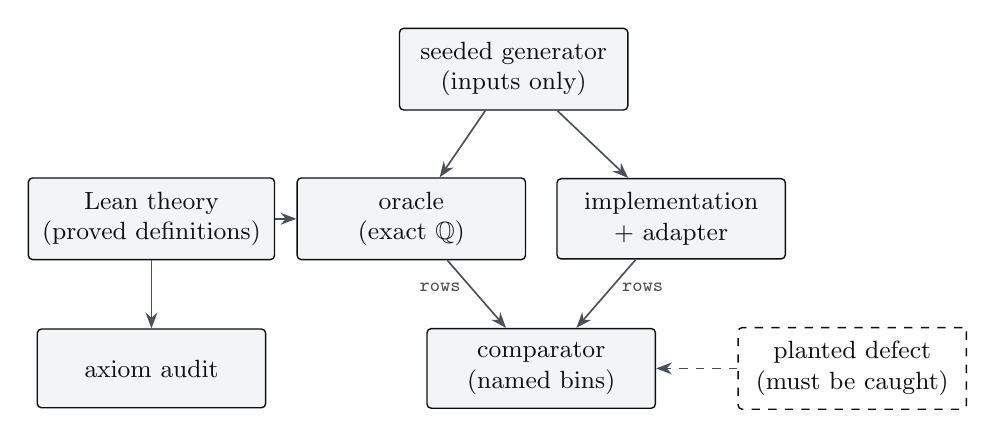
\begin{tikzpicture}[
  box/.style={draw=Ink, line width=0.5pt, fill=Surface, text=Ink, rounded corners=1.5pt,
    align=center, font=\small, inner sep=5pt, minimum height=10mm, minimum width=29mm},
  arr/.style={-{Stealth[length=2mm]}, line width=0.6pt, draw=InkMuted},
  lab/.style={font=\ttfamily\scriptsize, text=InkMuted}]
\node[box] (gen) at (4.6,1.9) {seeded generator\\(inputs only)};
\node[box] (theory) at (0,0) {Lean theory\\(proved definitions)};
\node[box] (oracle) at (3.3,0) {oracle\\(exact $\mathbb{Q}$)};
\node[box] (impl) at (6.6,0) {implementation\\+ adapter};
\node[box] (cmp) at (4.95,-1.9) {comparator\\(named bins)};
\node[box] (audit) at (0,-1.9) {axiom audit};
\node[box, dashed, fill=Background] (planted) at (8.9,-1.9) {planted defect\\(must be caught)};
\draw[arr] (gen) -- (oracle);
\draw[arr] (gen) -- (impl);
\draw[arr] (theory) -- (oracle);
\draw[arr] (theory) -- (audit);
\draw[arr] (oracle) -- node[left, lab, pos=0.4] {rows} (cmp);
\draw[arr] (impl) -- node[right, lab, pos=0.4] {rows} (cmp);
\draw[arr, dashed] (planted) -- (cmp);
\end{tikzpicture}
\caption{The measurement procedure. The generator never computes expected results;
those come only from the oracle.}
\label{fig:harness}
\end{figure}

The procedure follows \texttt{ledger-semantics} (\cref{fig:harness}). A seeded
generator writes case files containing inputs only. It favors the inputs where
implementations are known to have conventions: tied logits, words that are
themselves tokens, and merge tables with several splits of one string. A small
adapter per implementation runs the same cases and prints the oracle's row format.
The comparator places every case in exactly one named bin (agree, diverge, skipped
by either side, or missing), so nothing is dropped silently. Token rows are compared
as strings. Sampler rows require that a zero be matched by a zero and that nonzero
probabilities agree within $10^{-6}$, since llama.cpp stores logits in
\texttt{float32}. Each comparator is observed to fail: a planted defect, an adapter
that glues two tokens or one that inverts temperature, must be detected or the run
fails.

\paragraph{Tie divergences.} An implementation that keeps exactly $k$ tokens breaks
ties in its own order, which need not be the oracle's order by index. Every filter
treats tied tokens alike except for that choice, and tied tokens stay tied through
temperature and renormalization. Such an implementation must therefore agree with
the positional semantics up to a permutation of tied tokens. The harness checks
exactly this: the multiset of (logit, probability) pairs over the kept tokens must
equal that of the oracle's \texttt{q} rows. A divergence that fails this check is
reported as unexplained.

\begin{table}[t]
\centering\small
\caption{Measurements (\texttt{harness/run.sh 600}: four seeds of 600 cases each per
corpus). Lean 4.34.1, Mathlib v4.34.1, \texttt{tokenizers} 0.23.3, \texttt{tiktoken}
0.14.0, llama.cpp commit \texttt{a9d27ac} (2026-10-11).}
\label{tab:results}
\begin{tabularx}{\linewidth}{@{}>{\raggedright\arraybackslash}p{4.6cm}>{\raggedright\arraybackslash}X>{\raggedright\arraybackslash}X@{}}
\toprule
\qpth{Implementation} & \qpth{Compared against} & \qpth{Result}\\
\midrule
HF \texttt{tokenizers}, BPE, defaults & rule-rank BPE (\lean{bpe}) & 13{,}779 / 13{,}779 words identical\\
HF \texttt{tokenizers}, \lean{ignore_merges} & lookup, then rule-rank BPE & 13{,}779 / 13{,}779 identical\\
\texttt{tiktoken} & lookup, then concatenation-rank BPE & 13{,}779 / 13{,}779 identical\\
llama.cpp \lean{top_k}, \lean{top_p}, \lean{min_p}, \texttt{temp}, no ties & tie-keeping filters & 1{,}216 / 1{,}216 chains, $|\Delta p|\le5.1\times10^{-8}$\\
llama.cpp, with ties & tie-keeping, else positional & 939 + 245 / 1{,}184 chains; 0 unexplained\\
Planted defects (tokenizer, sampler) & --- & both detected\\
\bottomrule
\end{tabularx}
\end{table}

\Cref{tab:results} summarizes the results. Two findings came out of the
comparisons. First, \texttt{tiktoken} initially disagreed with the oracle's
concatenation-rank BPE on words that are themselves vocabulary tokens. The
disagreement was a convention, whole-word lookup. Following the
\texttt{ledger-semantics} rule that a divergence is either a defect in the
implementation or a convention the semantics has not yet recorded, we recorded it
as \lean{lookupFirst}, with its own theorems, after which agreement is exact.
Second, on the same random merge tables the two tokenizer libraries disagree with
each other on 439 of 13{,}779 words (3.2\%), and on 279 when Hugging Face uses
\lean{ignore_merges}. The oracle reproduces each library exactly, so every one of
these disagreements is predicted. \Cref{thm:bpeconv} states the condition under which
they cannot occur.

For sampling, llama.cpp agrees with the tie-keeping semantics on every tie-free
chain. On chains with ties, 245 of 1{,}184 diverge, and every one agrees with the
positional semantics up to a permutation of tied tokens. Some of these divergences
cascade: a tie cut by top-$k$ changes the renormalized masses that a later top-$p$
sees. A check that compared kept sets only after the fact would misclassify such
cases. Replaying the convention exactly classifies all of them.

% ===========================================================================
\section{Related work}

\paragraph{Formal methods for machine learning.} Most verification work on neural
networks proves properties of trained models, for example with SMT-based
methods~\cite{katz2017reluplex}. We verify the model-independent algorithms around
the model instead, and connect them to implementations through an oracle. The
denotational method follows Elliott~\cite{elliott2009denotational}. The use of a
proved semantics as a test oracle, the procedure of planted defects, and the
discipline of named skip bins follow \texttt{ledger-semantics}~\cite{ledgersemantics}.
Our category of finite stochastic maps is a special case of Fritz's Markov
categories~\cite{fritz2020markov}.

\paragraph{Tokenization.} Zouhar et al.\ give a formal analysis of BPE as an
optimization problem~\cite{zouhar2023bpe}. Gastaldi et al.\ treat tokenizers as
stochastic maps and study consistency of estimators~\cite{gastaldi2024foundations}.
Vieira et al.\ show how to turn token-level models into character-level
ones~\cite{vieira2024tokens}, which requires exactly the enumeration of
tokenizations we verify. Our no-compression theorem and the agreement criterion
between BPE conventions complement this work at the level of exact identities.

\paragraph{Decoding.} Top-$k$~\cite{fan2018hierarchical}, nucleus~\cite{holtzman2020curious}
and min-$p$~\cite{nguyen2025minp} sampling are usually specified by an algorithm over
sorted arrays, which leaves ties unspecified. \Cref{thm:topk} shows that this gap
cannot be closed by any symmetric rule. Speculative
sampling~\cite{leviathan2023speculative,chen2023speculative} is known to be lossless,
and its acceptance rate is the maximal-coupling bound~\cite{lindvall1992coupling}. Du et
al.\ characterize tightness measure-theoretically~\cite{du2023tight}. We give a
finite-depth statement and an explicit non-tight model.

\paragraph{Attention and inference systems.} Online softmax~\cite{milakov2018online}
underlies FlashAttention~\cite{dao2022flashattention} and its successors, and
KV caching is standard in serving systems~\cite{pope2023scaling,kwon2023vllm}. Our
contribution is the algebraic packaging, a commutative monoid with a free-monoid
homomorphism, and machine-checked proofs over arbitrary exponential characters.
Permutation equivariance of attention without positional encodings is
known~\cite{yun2020universal}.

\paragraph{Masked diffusion.} The time-independence of the optimal denoiser was
observed by Ou et al.~\cite{ou2025absorbing}, in the setting of
D3PM~\cite{austin2021d3pm}, MDLM~\cite{sahoo2024mdlm} and related
models~\cite{shi2024masked,nie2025llada}. We machine-check it, together with the
any-order chain rule and the inexactness of parallel unmasking.

% ===========================================================================
\section{Limitations}

Analysis on the reals enters only through exponential characters, and there is no
measure theory, so sampling and tightness are stated through finite quantities. The
oracle's temperature is restricted to $1/n$, which keeps softmax rational. The
theorems hold for every temperature, but the oracle cannot evaluate an irrational
softmax. Speculative decoding is proved for one drafted token. The sequence version
follows by induction and is not yet formalized. Nothing is proved about
floating-point arithmetic: implementations are compared with exact values within a
stated tolerance. A decision that lies exactly on a floating-point boundary could in
principle diverge, and none occurred in our runs. The diffusion theory covers
absorbing diffusion, not Gaussian diffusion. The chat protocol models tool calling in
its common request-and-result form, not any vendor's specification. The measurements
cover tokenizers and samplers; attention kernels, speculative decoders, chat
renderers and diffusion samplers are evaluated by the oracle but not yet compared
against implementations.

% ===========================================================================
\section{Conclusion}

The inference side of LLMs is small enough to be given a precise meaning and large
enough that its implementations disagree. A machine-checked semantics separates
what is meaning from what is convention. It proves which reorderings, cachings and
tilings are harmless, and it shows that some properties folklore expects, such as
symmetric exact top-$k$, compositional compressing tokenizers and unambiguous plain-text
templates, cannot exist. Connected to an exact oracle, the same definitions become
a test instrument. Every divergence it surfaces is either a defect in an
implementation or a convention that belongs in the semantics.

\paragraph{Availability.} The Lean development, oracle, harness, and recorded
measurement log accompany this paper.

\paragraph{Acknowledgments.} The structure of this work follows
\texttt{ledger-semantics} by John Wiegley. The formalization and harness were
developed with the assistance of an AI system (Claude, Anthropic).

% ===========================================================================
\begin{thebibliography}{99}\small

\bibitem{austin2021d3pm}
J.~Austin, D.~D. Johnson, J.~Ho, D.~Tarlow, and R.~van~den Berg.
\newblock Structured denoising diffusion models in discrete state-spaces.
\newblock In \emph{NeurIPS}, 2021.

\bibitem{chen2023speculative}
C.~Chen, S.~Borgeaud, G.~Irving, J.-B. Lespiau, L.~Sifre, and J.~Jumper.
\newblock Accelerating large language model decoding with speculative sampling.
\newblock arXiv:2302.01318, 2023.

\bibitem{dao2022flashattention}
T.~Dao, D.~Y. Fu, S.~Ermon, A.~Rudra, and C.~R{\'e}.
\newblock {FlashAttention}: Fast and memory-efficient exact attention with {IO}-awareness.
\newblock In \emph{NeurIPS}, 2022.

\bibitem{demoura2021lean4}
L.~de~Moura and S.~Ullrich.
\newblock The {Lean} 4 theorem prover and programming language.
\newblock In \emph{CADE-28}, 2021.

\bibitem{du2023tight}
L.~Du, L.~Torroba~Hennigen, T.~Pimentel, C.~Meister, J.~Eisner, and R.~Cotterell.
\newblock A measure-theoretic characterization of tight language models.
\newblock In \emph{ACL}, 2023.

\bibitem{elliott2009denotational}
C.~Elliott.
\newblock Denotational design with type class morphisms.
\newblock Technical Report 2009-01, LambdaPix, 2009.

\bibitem{fan2018hierarchical}
A.~Fan, M.~Lewis, and Y.~Dauphin.
\newblock Hierarchical neural story generation.
\newblock In \emph{ACL}, 2018.

\bibitem{fritz2020markov}
T.~Fritz.
\newblock A synthetic approach to {Markov} kernels, conditional independence and theorems on sufficient statistics.
\newblock \emph{Advances in Mathematics}, 370, 2020.

\bibitem{gastaldi2024foundations}
J.~L. Gastaldi, J.~Terilla, L.~Malagutti, B.~DuSell, T.~Vieira, and R.~Cotterell.
\newblock The foundations of tokenization: Statistical and computational concerns.
\newblock arXiv:2407.11606, 2024.

\bibitem{greshake2023injection}
K.~Greshake, S.~Abdelnabi, S.~Mishra, C.~Endres, T.~Holz, and M.~Fritz.
\newblock Not what you've signed up for: Compromising real-world {LLM}-integrated applications with indirect prompt injection.
\newblock In \emph{AISec}, 2023.

\bibitem{holtzman2020curious}
A.~Holtzman, J.~Buys, L.~Du, M.~Forbes, and Y.~Choi.
\newblock The curious case of neural text degeneration.
\newblock In \emph{ICLR}, 2020.

\bibitem{katz2017reluplex}
G.~Katz, C.~Barrett, D.~L. Dill, K.~Julian, and M.~J. Kochenderfer.
\newblock Reluplex: An efficient {SMT} solver for verifying deep neural networks.
\newblock In \emph{CAV}, 2017.

\bibitem{kwon2023vllm}
W.~Kwon, Z.~Li, S.~Zhuang, Y.~Sheng, L.~Zheng, C.~H. Yu, J.~E. Gonzalez, H.~Zhang, and I.~Stoica.
\newblock Efficient memory management for large language model serving with {PagedAttention}.
\newblock In \emph{SOSP}, 2023.

\bibitem{ledgersemantics}
J.~Wiegley.
\newblock ledger-semantics: Mathematical semantics of {Ledger}, the double-entry accounting tool.
\newblock \url{https://github.com/ledger/ledger-semantics}, 2026.

\bibitem{leviathan2023speculative}
Y.~Leviathan, M.~Kalman, and Y.~Matias.
\newblock Fast inference from transformers via speculative decoding.
\newblock In \emph{ICML}, 2023.

\bibitem{lindvall1992coupling}
T.~Lindvall.
\newblock \emph{Lectures on the Coupling Method}.
\newblock Wiley, 1992.

\bibitem{liu2023ring}
H.~Liu, M.~Zaharia, and P.~Abbeel.
\newblock Ring attention with blockwise transformers for near-infinite context.
\newblock arXiv:2310.01889, 2023.

\bibitem{mathlib2020}
The mathlib Community.
\newblock The {Lean} mathematical library.
\newblock In \emph{CPP}, 2020.

\bibitem{milakov2018online}
M.~Milakov and N.~Gimelshein.
\newblock Online normalizer calculation for softmax.
\newblock arXiv:1805.02867, 2018.

\bibitem{nguyen2025minp}
M.~N. Nguyen, A.~Baker, C.~Neo, A.~Roush, A.~Kirsch, and R.~Shwartz-Ziv.
\newblock Turning up the heat: Min-p sampling for creative and coherent {LLM} outputs.
\newblock In \emph{ICLR}, 2025.

\bibitem{nie2025llada}
S.~Nie, F.~Zhu, Z.~You, X.~Zhang, J.~Ou, J.~Hu, J.~Zhou, Y.~Lin, J.-R. Wen, and C.~Li.
\newblock Large language diffusion models.
\newblock arXiv:2502.09992, 2025.

\bibitem{ou2025absorbing}
J.~Ou, S.~Nie, K.~Xue, F.~Zhu, J.~Sun, Z.~Li, and C.~Li.
\newblock Your absorbing discrete diffusion secretly models the conditional distributions of clean data.
\newblock In \emph{ICLR}, 2025.

\bibitem{pope2023scaling}
R.~Pope, S.~Douglas, A.~Chowdhery, J.~Devlin, J.~Bradbury, J.~Heek, K.~Xiao, S.~Agrawal, and J.~Dean.
\newblock Efficiently scaling transformer inference.
\newblock In \emph{MLSys}, 2023.

\bibitem{rabe2021selfattention}
M.~N. Rabe and C.~Staats.
\newblock Self-attention does not need {$O(n^2)$} memory.
\newblock arXiv:2112.05682, 2021.

\bibitem{radford2019gpt2}
A.~Radford, J.~Wu, R.~Child, D.~Luan, D.~Amodei, and I.~Sutskever.
\newblock Language models are unsupervised multitask learners.
\newblock OpenAI technical report, 2019.

\bibitem{sahoo2024mdlm}
S.~S. Sahoo, M.~Arriola, Y.~Schiff, A.~Gokaslan, E.~Marroquin, J.~T. Chiu, A.~Rush, and V.~Kuleshov.
\newblock Simple and effective masked diffusion language models.
\newblock In \emph{NeurIPS}, 2024.

\bibitem{sennrich2016bpe}
R.~Sennrich, B.~Haddow, and A.~Birch.
\newblock Neural machine translation of rare words with subword units.
\newblock In \emph{ACL}, 2016.

\bibitem{shi2024masked}
J.~Shi, K.~Han, Z.~Wang, A.~Doucet, and M.~K. Titsias.
\newblock Simplified and generalized masked diffusion for discrete data.
\newblock In \emph{NeurIPS}, 2024.

\bibitem{vieira2024tokens}
T.~Vieira, B.~LeBrun, M.~Giulianelli, J.~L. Gastaldi, B.~DuSell, J.~Terilla, T.~J. O'Donnell, and R.~Cotterell.
\newblock From language models over tokens to language models over characters.
\newblock arXiv:2412.03719, 2024.

\bibitem{wolf2020transformers}
T.~Wolf et~al.
\newblock Transformers: State-of-the-art natural language processing.
\newblock In \emph{EMNLP: System Demonstrations}, 2020.

\bibitem{xiao2024sinks}
G.~Xiao, Y.~Tian, B.~Chen, S.~Han, and M.~Lewis.
\newblock Efficient streaming language models with attention sinks.
\newblock In \emph{ICLR}, 2024.

\bibitem{yun2020universal}
C.~Yun, S.~Bhojanapalli, A.~S. Rawat, S.~J. Reddi, and S.~Kumar.
\newblock Are transformers universal approximators of sequence-to-sequence functions?
\newblock In \emph{ICLR}, 2020.

\bibitem{zouhar2023bpe}
V.~Zouhar, C.~Meister, J.~L. Gastaldi, L.~Du, T.~Vieira, M.~Sachan, and R.~Cotterell.
\newblock A formal perspective on byte-pair encoding.
\newblock In \emph{Findings of ACL}, 2023.

\end{thebibliography}

\end{document}
"

\usepackage[a4paper,textwidth=15.4cm,textheight=23.6cm,top=3.0cm,headsep=0.9cm,footskip=1.2cm]{geometry}
\usepackage{amsmath,amssymb,amsthm,mathtools}
\usepackage{fontspec}
\usepackage{booktabs,tabularx,array}
\usepackage[protrusion=true,expansion=false]{microtype}
\usepackage[table]{xcolor}
\usepackage{graphicx}
\usepackage{fvextra}
\usepackage{enumitem}
\usepackage{caption}
\usepackage{titlesec}
\usepackage{fancyhdr}
\usepackage[most]{tcolorbox}
\usepackage{tikz}
\usetikzlibrary{arrows.meta}
\usepackage{hyperref}
\usepackage[nameinlink,capitalise]{cleveref}

% ---------------------------------------------------------------------------
%  Colour tokens
% ---------------------------------------------------------------------------
% Neutral foundation. Ink and Background invert between the two editions.
\ifqptdark
  \definecolor{Background}{HTML}{0B0C0E}
  \definecolor{Surface}{HTML}{16181B}
  \definecolor{Border}{HTML}{2B2E33}
  \definecolor{Ink}{HTML}{EDEEF0}
  \definecolor{InkMuted}{HTML}{A9AEB6}
  \definecolor{InkFaint}{HTML}{5A5F67}   % decoration only, never meaningful text
\else
  \definecolor{Background}{HTML}{FFFFFF}
  \definecolor{Surface}{HTML}{F3F4F5}
  \definecolor{Border}{HTML}{DADDE1}
  \definecolor{Ink}{HTML}{0E0F11}
  \definecolor{InkMuted}{HTML}{4B4F57}
  \definecolor{InkFaint}{HTML}{A3A7AE}   % decoration only, never meaningful text
\fi
% Paradigm colours: fixed in both editions, semantic only.
\definecolor{Quantum}{HTML}{5BAD1E}
\definecolor{Photonic}{HTML}{F0AB00}
\definecolor{Thermodynamic}{HTML}{E8690A}
\definecolor{Ternary}{HTML}{8A8A8A}
\definecolor{Bio}{HTML}{1AAB7C}

\ifqptdark\pagecolor{Background}\fi

% ---------------------------------------------------------------------------
%  Typography
% ---------------------------------------------------------------------------
\setmainfont{Inter}[
  Path=fonts/, Extension=.otf, Scale=0.94,
  UprightFont=*-Regular, ItalicFont=*-Italic,
  BoldFont=*-SemiBold, BoldItalicFont=*-SemiBoldItalic]
\setmonofont{IBMPlexMono}[
  Path=fonts/, Extension=.ttf, Scale=MatchLowercase,
  UprightFont=*-Regular, ItalicFont=*-Italic, BoldFont=*-SemiBold]
\newfontfamily\qptdisplay{SpaceGrotesk}[
  Path=fonts/, Extension=.otf, UprightFont=*-Medium, BoldFont=*-Bold]
\newfontfamily\qptdisplaylight{SpaceGrotesk}[
  Path=fonts/, Extension=.otf, UprightFont=*-Regular]
\newfontfamily\qptlabelfont{IBMPlexMono}[
  Path=fonts/, Extension=.ttf, Scale=MatchLowercase, UprightFont=*-Medium,
  LetterSpace=6]
\setsansfont{Inter}[
  Path=fonts/, Extension=.otf, Scale=0.94,
  UprightFont=*-Regular, ItalicFont=*-Italic,
  BoldFont=*-SemiBold, BoldItalicFont=*-SemiBoldItalic]
\linespread{1.16}
\setlength{\emergencystretch}{2.5em}
\AtBeginDocument{\raggedright\setlength{\parindent}{0pt}}
\setlength{\parindent}{0pt}
\setlength{\parskip}{0.55em}

% A label: IBM Plex Mono, upper case, tracked.
\newcommand{\qptlabel}[1]{{\qptlabelfont\footnotesize\MakeUppercase{#1}}}
% Technical names (Lean declarations, files) in IBM Plex Mono.
\newcommand{\lean}[1]{\texttt{\detokenize{#1}}}
\newcommand{\leanref}[1]{\par\smallskip\noindent
  {\ttfamily\footnotesize\upshape\raggedright\color{InkMuted}LEAN\enspace #1\par}}

% Ink is the normal colour everywhere, including floats, heads and footnotes.
\makeatletter
\AtBeginDocument{\color{Ink}\global\let\default@color\current@color}
\makeatother

% ---------------------------------------------------------------------------
%  Mathematical notation
% ---------------------------------------------------------------------------
\newcommand{\K}{\Bbbk}
\newcommand{\Dist}{\mathrm{Dist}}
\newcommand{\restr}[2]{#1|_{#2}}
\newcommand{\topk}{\mathrm{TopK}}
\newcommand{\topp}{\mathrm{TopP}}
\newcommand{\minp}{\mathrm{MinP}}
\newcommand{\sharpen}{\mathrm{sharpen}}
\newcommand{\abv}{\mathrm{above}}
\newcommand{\tv}{\mathrm{tv}}
\newcommand{\dec}{\mathrm{dec}}
\newcommand{\enc}{\mathrm{enc}}
\newcommand{\softmax}{\mathrm{softmax}}
\newcommand{\attend}{\mathrm{attend}}
\newcommand{\Iv}[1]{[\![#1]\!]}
\newcommand{\Mask}{\bot}

% ---------------------------------------------------------------------------
%  Headings: section numbers as labels, titles in Space Grotesk
% ---------------------------------------------------------------------------
\makeatletter
\newcommand{\qptsecnum}[1]{{\qptlabelfont\small\color{InkMuted}\two@digits{#1}}}
\makeatother
\titleformat{\section}
  {\qptdisplay\fontsize{14.5}{18}\selectfont\color{Ink}}
  {\qptsecnum{\value{section}}}{0.9em}{}
\titleformat{name=\section,numberless}
  {\qptdisplay\fontsize{14.5}{18}\selectfont\color{Ink}}{}{0pt}{}
\titlespacing*{\section}{0pt}{1.9em}{0.7em}
\titleformat{\paragraph}[runin]
  {\qptdisplay\normalsize\color{Ink}}{}{0pt}{}
\titlespacing*{\paragraph}{0pt}{0.9em}{0.6em}

% ---------------------------------------------------------------------------
%  Statements
% ---------------------------------------------------------------------------
\newtheoremstyle{qpt}
  {0.9em}{0.9em}
  {\normalfont}{}
  {\qptlabelfont\footnotesize}{}
  {\newline}
  {\MakeUppercase{\thmname{#1}\thmnumber{~#2}}%
   \thmnote{\enspace{\qptdisplay\normalsize\color{Ink}#3}}}
\theoremstyle{qpt}
\newtheorem{theorem}{Theorem}
\newtheorem{proposition}[theorem]{Proposition}
\newtheorem{corollary}[theorem]{Corollary}
\newtheorem{lemma}[theorem]{Lemma}
\newtheorem{definition}[theorem]{Definition}
\newtheorem{remark}[theorem]{Remark}

% Proofs: a tracked label and a neutral end mark.
\makeatletter
\renewcommand{\qedsymbol}{{\color{InkMuted}\rule{0.5em}{0.5em}}}
\renewenvironment{proof}[1][Proof]{\par\pushQED{\qed}\normalfont\topsep0.5em\relax
  \trivlist\item[\hskip\labelsep\qptlabel{#1}\hspace{0.6em}]\ignorespaces}
  {\popQED\endtrivlist\@endpefalse}
\makeatother

% ---------------------------------------------------------------------------
%  Code: IBM Plex Mono on a neutral surface, with a hairline on the left
% ---------------------------------------------------------------------------
\tcbset{colupper=Ink, collower=Ink}
\tcbset{qptcode/.style={enhanced, colback=Surface, colframe=Surface,
  boxrule=0pt, arc=0pt, left=9pt, right=8pt, top=5pt, bottom=5pt,
  borderline west={1.2pt}{0pt}{InkFaint}, before skip=0.7em, after skip=0.7em}}
\newenvironment{leancode}
  {\VerbatimEnvironment\begin{tcolorbox}[qptcode]%
   \begin{Verbatim}[fontsize=\small,commandchars=\\\{\},
     codes={\catcode`\$=3\catcode`\^=7},formatcom=\color{Ink}]}
  {\end{Verbatim}\end{tcolorbox}}
\newenvironment{casecode}
  {\VerbatimEnvironment\begin{tcolorbox}[qptcode,before skip=0pt,after skip=0pt]%
   \begin{Verbatim}[fontsize=\footnotesize,formatcom=\color{Ink}]}
  {\end{Verbatim}\end{tcolorbox}}

% ---------------------------------------------------------------------------
%  Floats, tables, captions
% ---------------------------------------------------------------------------
\DeclareCaptionLabelFormat{qpt}{\qptlabel{#1~#2}}
\DeclareCaptionLabelSeparator{qptsep}{\quad}
\captionsetup{labelformat=qpt, labelsep=qptsep, font={small,color=Ink},
  justification=raggedright, singlelinecheck=false, skip=6pt}
\newcommand{\qpth}[1]{\qptlabel{#1}}
\arrayrulecolor{Ink}
\setlength{\heavyrulewidth}{0.7pt}
\setlength{\lightrulewidth}{0.35pt}
\renewcommand{\arraystretch}{1.22}

% ---------------------------------------------------------------------------
%  Running heads
% ---------------------------------------------------------------------------
\pagestyle{fancy}
\fancyhf{}
\fancyhead[L]{{\color{Ink}\qptlabel{Machine-checked semantics of LLM inference}}}
\fancyhead[R]{{\color{Ink}\qptlabel{D. Arango Sohm}}}
\fancyfoot[R]{{\ttfamily\small\color{InkMuted}\thepage}}
\renewcommand{\headrule}{{\color{Border}\hrule height 0.4pt}\vspace{-0.4pt}}
\renewcommand{\headrulewidth}{0.4pt}
\fancypagestyle{qptfirst}{\fancyhf{}%
  \fancyfoot[R]{{\ttfamily\small\color{InkMuted}\thepage}}%
  \renewcommand{\headrulewidth}{0pt}\renewcommand{\headrule}{}}

% ---------------------------------------------------------------------------
%  Links and references: neutral, never accent-coloured text
% ---------------------------------------------------------------------------
\hypersetup{colorlinks=true, linkcolor=Ink, citecolor=Ink, urlcolor=Ink,
  pdftitle={A Machine-Checked Semantics of LLM Inference},
  pdfauthor={Daniel Arango Sohm},
  pdfsubject={Formal semantics of large language model inference in Lean 4},
  pdfkeywords={Lean 4, Mathlib, formal verification, LLM inference, sampling,
    tokenization, attention, speculative decoding, diffusion language models}}
\makeatletter
\renewcommand{\@biblabel}[1]{{\ttfamily\color{InkMuted}[#1]}}
\renewcommand{\@cite}[2]{{\ttfamily[#1\if@tempswa, #2\fi]}}
\makeatother
\renewcommand{\refname}{References}

\setlist{itemsep=2pt, topsep=4pt}
\setlist[itemize]{label={\color{InkMuted}\textbullet}}

\begin{document}
\thispagestyle{qptfirst}

% ----------------------------------------------------------------- masthead
\noindent
\begin{minipage}[c]{0.5\linewidth}
  \includegraphics[height=1.9cm]{qpt-logo.png}
\end{minipage}%
\begin{minipage}[c]{0.5\linewidth}\raggedleft
  \qptlabel{Preprint}\\[2pt]
  \qptlabel{October 2026}
\end{minipage}

\vspace{1.6em}
{\color{Border}\rule{\linewidth}{0.4pt}}
\vspace{1.1em}

{\qptdisplay\fontsize{25}{29.5}\selectfont\color{Ink}
A Machine-Checked Semantics\\ of LLM Inference\par}
\vspace{0.55em}
{\qptdisplaylight\fontsize{13}{17}\selectfont\color{InkMuted}
Sampling, Attention, Tokenization, Chat, Decoding,\\ and Diffusion in Lean~4\par}

\vspace{1.5em}
{\large\bfseries Daniel Arango Sohm}\par
\vspace{0.15em}
{\color{InkMuted}Universidad EAFIT, Medellín, Colombia\\
Former member of the QPT team}\par

\vspace{1.4em}
% ----------------------------------------------------------------- abstract
\begin{tcolorbox}[enhanced, colback=Surface, colframe=Surface, colupper=Ink, boxrule=0pt,
  arc=0pt, left=12pt, right=12pt, top=9pt, bottom=10pt]
\qptlabel{Abstract}\par\vspace{0.35em}
{\small
The inference side of a large language model is a stack of small algorithms:
tokenizers, attention kernels, key--value caches, sampling filters, speculative
decoders, chat templates, and diffusion samplers. Each has several independent
implementations, and those implementations are usually tested against one another
rather than against a definition. We give these components a single mathematical
semantics, formalized in Lean~4 against Mathlib. The development comprises about
4{,}600 lines and 270 named theorems, and every declaration depends only on Lean's
three standard axioms. It proves the exact algebra of sampling filters, the
losslessness and optimality of speculative sampling, and the correctness of
key--value caching and of FlashAttention-style online softmax as a commutative
monoid. It proves that byte-pair encoding is lossless under every merge priority,
together with a decidable criterion for when the Hugging Face and \texttt{tiktoken}
conventions agree, a protocol checker for tool calls, and the time-independence of
the masked-diffusion denoiser. It also proves six negative results. No sampling
rule that treats tokens symmetrically can always keep exactly $k$ tokens. No
tokenizer that compresses can respect concatenation. Every chat template that writes
its role markers in the content alphabet is ambiguous. No transformer without
positional information can copy a fixed position. An autoregressive model need not
define a distribution over strings. Parallel unmasking in diffusion is inexact.
From the same definitions we build an executable oracle that evaluates test cases in
exact rational arithmetic, and a harness that measures implementations against it.
On 2{,}400 random merge tables, Hugging Face \texttt{tokenizers} and
\texttt{tiktoken} each agree with the oracle on all 13{,}779 test words, while
disagreeing with each other on 3.2\% of them. On 2{,}400 random sampler chains,
every divergence of llama.cpp from the tie-keeping semantics is accounted for
exactly by the positional semantics that the impossibility theorem forces.
\par}
\end{tcolorbox}

\vspace{0.3em}
\noindent\qptlabel{Keywords}\enspace{\small Lean~4 · Mathlib · formal verification ·
LLM inference · sampling · tokenization · attention · speculative decoding ·
diffusion language models}

\vspace{0.4em}
{\color{Border}\rule{\linewidth}{0.4pt}}

% ===========================================================================
\section{Introduction}

A deployed language model is a function from parameters and a context to a
distribution over tokens. Turning that distribution into text requires more
machinery. A tokenizer maps strings to token sequences. Attention kernels compute
the model's reads over a cached context. A chain of sampling filters reshapes the
next-token distribution. A speculative decoder may verify drafted tokens, a chat
template linearizes a conversation, and a diffusion sampler may unmask several
positions at once. Each of these components exists in many implementations, such as
Hugging Face \texttt{transformers} and \texttt{tokenizers}~\cite{wolf2020transformers},
\texttt{tiktoken}, vLLM~\cite{kwon2023vllm}, and llama.cpp. Their tests mostly
compare one implementation with another, or with remembered behavior.

This paper follows a different discipline, \emph{denotational design}~\cite{elliott2009denotational}.
One first says precisely what a thing means, then requires every operation to
preserve that meaning, and lets the implementation be whatever the equations force
it to be. The approach is that of \texttt{ledger-semantics}~\cite{ledgersemantics},
which formalizes double-entry accounting in Lean and uses the result as a test oracle
for the C++ Ledger program. We apply it to LLM inference. A sampling filter means
conditioning a distribution on a set. A KV-cached decoder means causal attention over
the whole prefix. A FlashAttention kernel means a softmax-weighted average. A chat
template means an injective encoding of a transcript. The theorems state when an
implementation preserves that meaning, and several of them state that no
implementation can.

\paragraph{Contributions.}
\begin{itemize}[leftmargin=*,itemsep=2pt]
\item A Lean~4 formalization against Mathlib~\cite{mathlib2020,demoura2021lean4}
  of sampling, speculative decoding, softmax and attention, tokenization, chat
  transcripts, autoregressive decoding, and masked diffusion
  (\cref{sec:foundations,sec:sampling,sec:spec,sec:attention,sec:tokenization,sec:chat,sec:decoding,sec:diffusion}).
  All definitions are stated over an arbitrary linearly ordered field, so one proof
  covers the real numbers of the literature and the exact rationals of the oracle.
\item Positive results in a common framework. They include the algebra of
  sampling filters, the optimality of speculative sampling, an online-softmax
  commutative monoid, a generic correctness theorem for BPE with a decidable
  agreement criterion between the two conventions in use, a protocol checker for
  tool calls, and the any-order chain rule for masked diffusion.
\item Six negative results that explain design constraints visible across
  implementations (\cref{sec:negative}).
\item An executable oracle that evaluates case files under the proved
  definitions in exact arithmetic, and a measurement of Hugging Face
  \texttt{tokenizers}, \texttt{tiktoken}, and llama.cpp against it (\cref{sec:oracle,sec:measure}).
\end{itemize}

Several of the positive results are known: losslessness of speculative
sampling~\cite{leviathan2023speculative,chen2023speculative}, correctness of online
softmax~\cite{milakov2018online,dao2022flashattention}, time-independence of the
absorbing-diffusion posterior~\cite{ou2025absorbing}, and the role of permutation
equivariance~\cite{yun2020universal}. Our contribution for these is a machine-checked
statement in one framework, connected to an oracle. To our knowledge the
following are not stated elsewhere in the form given here: the impossibility of
symmetric exact top-$k$ and nucleus selection, the no-compression theorem for
homomorphic tokenizers, the ambiguity of every in-band chat template, and the
decidable agreement criterion between merge-rule and concatenation-rank BPE.

% ===========================================================================
\section{Method and trust base}\label{sec:method}

The development is a Lean~4 library (Lean 4.34.1, Mathlib v4.34.1) of eleven
theory modules and two executable modules (\cref{tab:modules}). It is built with
warnings promoted to errors, so an unproved theorem (\lean{sorry}) fails the build.
A separate audit program walks every declaration in the library, 853 in all, and
fails unless each depends only on propositional extensionality, the axiom of choice,
and quotient soundness. The audit has been observed to fail: a planted proof by
\lean{native_decide}, which introduces an auxiliary axiom trusting compiled code, is
rejected. The warnings-as-errors build alone does not catch it. Concrete
counterexamples are therefore proved by \lean{decide}, whose certificate the kernel
checks by evaluation.

\begin{table}[t]
\centering\small
\caption{Modules of the development. Lines and named theorems and lemmas per module.}
\label{tab:modules}
\begin{tabularx}{\linewidth}{@{}l>{\raggedright\arraybackslash}X>{\ttfamily}r>{\ttfamily}r@{}}
\toprule
\qpth{Module} & \qpth{Content} & \qpth{Lines} & \qpth{Thms} \\
\midrule
\lean{Dist} & finite distributions, conditioning, total variation, $\mathsf{FinStoch}$ & 383 & 34\\
\lean{Sampling} & top-$k$, top-$p$, min-$p$, temperature, ties, inverse CDF & 732 & 46\\
\lean{Counterexamples} & kernel-checked failures of sampler laws & 52 & 4\\
\lean{Speculative} & speculative sampling, couplings & 194 & 17\\
\lean{Softmax} & exponential characters, masking, temperature & 220 & 23\\
\lean{Attention} & equivariance, causality, KV cache, online softmax & 573 & 38\\
\lean{Real} & $\exp$ as a character; textbook restatements & 51 & 4\\
\lean{Tokenization} & free-monoid decoding, BPE conventions, enumeration & 860 & 49\\
\lean{Chat} & tool-call protocol, rendering & 440 & 21\\
\lean{Decoding} & mass conservation, tightness, greedy decoding & 245 & 15\\
\lean{Diffusion} & masked diffusion, posterior, chain rule & 379 & 18\\
\lean{Oracle}, \lean{Driver} & case parsing and exact evaluation & 465 & 1\\
\midrule
Total & & 4{,}594 & 270\\
\bottomrule
\end{tabularx}
\end{table}

\paragraph{Numbers.} Every probability lives in an arbitrary field $\K$ with a
compatible linear order (\lean{[Field K] [LinearOrder K] [IsStrictOrderedRing K]}).
The oracle instantiates $\K=\mathbb{Q}$, so its arithmetic is exact. The analytic
statements instantiate $\K=\mathbb{R}$. No measure theory is used. Sampling is made
precise through interval statements (\cref{thm:invcdf}), and tightness through
masses at finite depth (\cref{sec:decoding}).

% ===========================================================================
\section{Foundations}\label{sec:foundations}

\begin{definition}[Finite distribution]
For a finite type $\alpha$, $\Dist_\K(\alpha)$ is the type of functions
$p:\alpha\to\K$ with $p(a)\ge 0$ for all $a$ and $\sum_a p(a)=1$.
\leanref{\lean{Dist}}
\end{definition}

\begin{leancode}
structure Dist ($\K$ : Type u) [Field $\K$] [LinearOrder $\K$] [IsStrictOrderedRing $\K$]
    ($\alpha$ : Type v) [Fintype $\alpha$] where
  prob : $\alpha$ $\to$ $\K$
  nonneg : $\forall$ a, 0 $\le$ prob a
  sum_eq_one : $\sum$ a, prob a = 1
\end{leancode}

The single operation through which masks, filters and grammar constraints act is
conditioning. For $S\subseteq\alpha$ with $p(S)>0$, write
$\restr{p}{S}(a)=\Iv{a\in S}\,p(a)/p(S)$ (\lean{Dist.restrict}).

\begin{lemma}[Conditioning]\label{lem:restrict}
$\restr{(\restr{p}{S})}{T}=\restr{p}{S\cap T}$ whenever the masses involved are
positive. Moreover $\restr{p}{S}=\restr{p}{S'}$ whenever $S$ and $S'$ contain the same
outcomes of positive probability.
\leanref{\lean{restrict_restrict}, \lean{restrict_congr}}
\end{lemma}

The finite distribution monad (point masses and \lean{bind}) satisfies the monad
laws. Finite types and stochastic maps $\alpha\to\Dist_\K(\beta)$ form a category
$\mathsf{FinStoch}_\K$, given as an instance of Mathlib's \lean{Category} whose
composition is Kleisli composition (\lean{FinStoch.category}). Total variation is
$\tv(p,q)=\sum_a\max(0,p(a)-q(a))$. We prove
$\tv(p,q)=\tfrac12\sum_a|p(a)-q(a)|$, $\sum_a\min(p(a),q(a))=1-\tv(p,q)$, and
$\tv(p,q)=0\iff p=q$.

% ===========================================================================
\section{Sampling}\label{sec:sampling}

Let $V$ be a finite vocabulary and $p:V\to\K$. Write
$\abv_p(v)=\{u: p(v)<p(u)\}$ for the tokens strictly preferred to $v$. The three
standard filters keep the sets
\begin{gather*}
\topk_k(p)=\{v: |\abv_p(v)|<k\},\qquad
\minp_m(p)=\{v:\forall u,\; m\,p(u)\le p(v)\},\\
\topp_P(p)=\Bigl\{v: \textstyle\sum_{u\in\abv_p(v)}p(u)<P\Bigr\},
\end{gather*}
and the filtered distribution is the conditioning $\restr{p}{S}$ on the kept set
$S$. For distinct probabilities, $\topp_P$ is the usual rule ``sort in descending
order and keep the shortest prefix whose mass reaches $P$''. With ties, all three
keep every tied token. Temperature $1/n$ is
$\sharpen_n(p)(v)=p(v)^n/\sum_u p(u)^n$, which stays inside $\mathbb{Q}$. In
\cref{sec:attention} we show that it equals $\softmax(n\cdot z)$ when
$p=\softmax(z)$. Every kept set contains a most probable token, provided $k\ge1$,
$P>0$ and $m\le1$, so no filter can produce an empty distribution.

\begin{theorem}[Sampler algebra]\label{thm:algebra}
For $k,k'\ge1$, $m,m'\le1$ and $n\ge1$, and writing filters in the order they are
applied,
\begin{enumerate}[label=(\roman*),itemsep=1pt]
\item top-$k$ then top-$k'$ equals top-$\min(k,k')$;
\item min-$m$ then min-$m'$ equals min-$\max(m,m')$; in particular both filters are idempotent;
\item top-$k$ and min-$m$ commute;
\item top-$k$ and temperature $1/n$ commute.
\end{enumerate}
\leanref{\lean{topK_topK}, \lean{minP_minP}, \lean{topK_minP_comm}, \lean{topK_sharpen_comm}}
\end{theorem}

\begin{proof}[Proof sketch]
All three kept sets are \emph{upward closed}: if $v$ is kept and $p(v)<p(u)$, then
$u$ is kept. Conditioning on an upward-closed set $S$ leaves $\abv(v)$ unchanged for
$v\in S$ (\lean{above_restrict}), and min-$p$ is insensitive to conditioning on a set
that contains a maximizer (\lean{minP_restrict_iff}). Each identity then reduces,
through \cref{lem:restrict}, to an equality of kept sets. For (iv), $x\mapsto x^n$
is strictly increasing on $[0,\infty)$, and top-$k$ depends only on the order of the
scores (\lean{topKSet_congr}).
\end{proof}

The laws one might expect beyond \cref{thm:algebra} are false. With
$p_0=(\tfrac12,\tfrac3{10},\tfrac15)$, the kernel evaluates the following
(\lean{Counterexamples}).

\begin{proposition}[Failed laws]\label{prop:counter}
\leavevmode\vspace{-0.5\baselineskip}
\begin{enumerate}[label=(\roman*),itemsep=1pt]
\item Top-$p$ is not idempotent: one pass of $\topp_{3/5}$ gives token~1 the probability $\tfrac38$, and a second pass gives it~$0$.
\item Top-$p$ does not commute with top-$k$: top-$p$ then top-2 leaves token~1 at $\tfrac38$, while top-2 then top-$p$ removes it.
\item Top-$p$ does not commute with temperature $\tfrac12$: token~1 ends at $\tfrac9{34}$ in one order and at $0$ in the other.
\item Min-$p$ ($m=\tfrac12$) does not commute with temperature $\tfrac12$, with the same numbers.
\end{enumerate}
\end{proposition}

A sampler chain may therefore reorder top-$k$, min-$p$ and temperature only as
\cref{thm:algebra} allows, and may not move top-$p$ at all.

\paragraph{Ties.} Implementations differ on ties, and the difference is forced.
Call a selection rule $\mathrm{sel}:(V\to\K)\to\mathcal{P}(V)$ \emph{equivariant} if
$\mathrm{sel}(p\circ\sigma^{-1})=\sigma[\mathrm{sel}(p)]$ for every permutation
$\sigma$ of $V$, that is, if relabeling the tokens relabels the output.

\begin{theorem}[No symmetric exact top-$k$]\label{thm:topk}
Let $0<k<|V|$. No equivariant selection rule satisfies $|\mathrm{sel}(p)|=k$ for
every distribution $p$.
\leanref{\lean{no_equivariant_exact_topK}}
\end{theorem}
\begin{proof}
On the uniform distribution $u$ we have $u\circ\sigma^{-1}=u$ for every $\sigma$, so
$\mathrm{sel}(u)$ is invariant under all permutations. If it contains some $v$, then
for any $w$ the transposition $(v\,w)$ maps $v$ to $w$, so it contains $w$ too.
Hence $\mathrm{sel}(u)$ is either empty or all of $V$, and neither has $k$ elements.
\end{proof}

\begin{leancode}
theorem no_equivariant_exact_topK [DecidableEq V] \char123{}k : $\mathbb{N}$\char125{}
    (hk0 : 0 < k) (hkn : k < Fintype.card V)
    (sel : (V $\to$ $\K$) $\to$ Finset V) (hsel : Equivariant sel) :
    $\neg$ $\forall$ d : Dist $\K$ V, (sel d.prob).card = k
\end{leancode}

\begin{theorem}[No symmetric smallest nucleus]
Let $V$ be nonempty and $0<P\le1-1/|V|$. No equivariant rule returns, for every
distribution, a set of minimum cardinality among those of mass at least~$P$.
\leanref{\lean{no_equivariant_exact_nucleus}}
\end{theorem}

The tie-keeping filters are equivariant (\lean{topKSet_equivariant}). The other
option is to break ties by position. Define $u\prec_p v$ if $p(u)>p(v)$, or if
$p(u)=p(v)$ and $u<v$, and let the positional filters count predecessors under
$\prec_p$ instead of $\abv_p$ (\lean{Dist.topKPos}, \lean{Dist.topPPos}).

\begin{theorem}[Positional tie-breaking]
Positional top-$k$ keeps exactly $\min(k,|V|)$ tokens. If $p$ is injective, the
positional and tie-keeping filters coincide. For $0<k<|V|$, positional top-$k$ is
not equivariant.
\leanref{\lean{card_topKPosSet}, \lean{topKPosSet_eq_of_injective}, \lean{topPPosSet_eq_of_injective}, \lean{topKPosSet_not_equivariant}}
\end{theorem}

An implementation must therefore choose between keeping exactly $k$ tokens and
treating tokens symmetrically. Hugging Face \texttt{transformers} (read from the
source of version 5.19.0) keeps ties in top-$k$, since it removes only scores
strictly below the $k$-th largest, but breaks them by sort position in top-$p$.
llama.cpp breaks ties by position in both, as measured in \cref{sec:measure}.

\begin{theorem}[Inverse-CDF sampling]\label{thm:invcdf}
Let $F(i)=\sum_{j<i}p(j)$ on $V=\{0,\dots,n-1\}$ and let $\iota(u)$ be the least $i$
with $u<F(i+1)$. For $0\le u<1$, $\iota(u)=i\iff F(i)\le u<F(i+1)$, and
$F(i+1)-F(i)=p(i)$. A uniform $u$ therefore selects $i$ with probability $p(i)$.
\leanref{\lean{invCdf_eq_iff}, \lean{cdf_interval_length}}
\end{theorem}

% ===========================================================================
\section{Speculative decoding}\label{sec:spec}

A draft model proposes $x\sim q$. The target, with distribution $p$, accepts with
probability $a(x)=\min(1,p(x)/q(x))$, and on rejection a token is drawn from the
residual $r=(p-q)^+/\tv(p,q)$~\cite{leviathan2023speculative,chen2023speculative}.
We define the joint law of (draft, emitted token) exactly as the algorithm runs,
\[
\pi(x,y)=q(x)\bigl(a(x)\,\Iv{y=x}+(1-a(x))\,r(y)\bigr).
\]

\begin{theorem}[Speculative sampling]
\leavevmode\vspace{-0.5\baselineskip}
\begin{enumerate}[label=(\roman*),itemsep=1pt]
\item The draft has law $q$: $\sum_y\pi(x,y)=q(x)$.
\item \emph{Losslessness}: the emitted token has law $p$: $\sum_x\pi(x,y)=p(y)$.
\item The acceptance probability is $\sum_x q(x)a(x)=1-\tv(p,q)$, and the emitted token equals the draft with the same probability.
\item \emph{Optimality}: every coupling $\gamma$ of $q$ and $p$ has $\sum_x\gamma(x,x)\le1-\tv(p,q)$.
\end{enumerate}
\leanref{\lean{specJoint_fst}, \lean{specJoint_snd}, \lean{accept_rate}, \lean{specJoint_diag}, \lean{coupling_le}, \lean{spec_optimal}}
\end{theorem}
\begin{proof}[Proof sketch]
Since $q(x)a(x)=\min(p(x),q(x))$, the total rejection probability is $\tv(p,q)$,
and a rejected draft is never re-emitted, because $r(x)=0$ whenever $q(x)>p(x)$. For (iv),
$\gamma(x,x)\le\min(q(x),p(x))$ by the marginal constraints. This is the classical
coupling inequality~\cite{lindvall1992coupling}.
\end{proof}

Because any lossless rule for verifying one drafted token is a coupling, (iv) shows
that speculative sampling has the highest acceptance rate any such rule can achieve.

% ===========================================================================
\section{Softmax and attention}\label{sec:attention}

\begin{definition}[Exponential character]
An \emph{exponential character} from an ordered additive group $G$ of scores into
$\K$ is a strictly increasing map $E:G\to\K$ with $E(a)>0$ and $E(a+b)=E(a)E(b)$.
For $z:\iota\to G$, $\softmax_E(z)_i=E(z_i)/\sum_jE(z_j)$.
\leanref{\lean{ExpChar}}
\end{definition}

$\exp:\mathbb{R}\to\mathbb{R}$ is a character (\lean{ExpChar.real}). So is
$z\mapsto2^z:\mathbb{Z}\to\mathbb{Q}$ (\lean{ExpChar.base2}), which the oracle uses
to evaluate softmax with no rounding. Every result in this section holds for every
character, and so for both.

\begin{theorem}[Softmax]\label{thm:softmax}
\leavevmode\vspace{-0.5\baselineskip}
\begin{enumerate}[label=(\roman*),itemsep=1pt]
\item $\softmax_E(z+c)=\softmax_E(z)$; this licenses subtracting the maximum logit.
\item $\softmax_E(z)_i<\softmax_E(z)_j\iff z_i<z_j$.
\item \emph{Masking is conditioning}: setting logits outside $S$ to $-\infty$ and taking softmax gives $\restr{\softmax_E(z)}{S}$.
\item For $G$ a field and $T>0$, $\topk_k(\softmax_E(z/T))=\topk_k(z)$.
\item $\softmax_E(n\cdot z)=\sharpen_n(\softmax_E(z))$.
\end{enumerate}
\leanref{\lean{softmax_add_const}, \lean{softmax_lt_iff}, \lean{softmaxOn_eq_restrict}, \lean{topK_temperature}, \lean{softmax_nsmul}}
\end{theorem}

\paragraph{One read.} $\attend(s,v)=\sum_j\softmax_E(s)_j\,v_j$ for scores $s$ and
values $v_j$ in a $\K$-module.

\begin{theorem}[Convexity]
For every linear functional $\varphi$ and constant $c$, if $\varphi(v_j)\le c$ for all
$j$ then $\varphi(\attend(s,v))\le c$. If every $v_j=m$, then $\attend(s,v)=m$ for
every $s$.
\leanref{\lean{attend_convex}, \lean{attend_const}}
\end{theorem}

The second statement says attention cannot abstain. Its weights always sum to one,
which is the property that motivates attention-sink tokens~\cite{xiao2024sinks}.

\paragraph{Permutation equivariance.} A map $f:(\iota\to X)\to(\iota\to Y)$ is
equivariant if $f(x\circ\sigma)=f(x)\circ\sigma$ for every permutation~$\sigma$.

\begin{theorem}[Equivariance]
Self-attention with any score function and no positional information is
equivariant. So is any block $y=x+\sum_h\mathrm{attn}_h(\mathrm{norm}\,x)$,
$\mathrm{out}=y+\mathrm{mlp}(\mathrm{norm}\,y)$, and any stack of such blocks.
\leanref{\lean{selfAttn_equivariant}, \lean{block_equivariant}, \lean{stack_equivariant}}
\end{theorem}

\begin{theorem}[Positional information is necessary]\label{thm:nofirst}
If $\iota$ has two distinct positions $i_0\ne i_1$ and $X$ has two distinct elements,
no equivariant $f:(\iota\to X)\to(\iota\to X)$ satisfies $f(x)_i=x_{i_0}$ for all $x$ and $i$.
\leanref{\lean{no_equivariant_first}}
\end{theorem}
\begin{proof}
Let $x_{i_0}=a$ and $x_i=b$ elsewhere, and let $\sigma=(i_0\,i_1)$. Then
$f(x\circ\sigma)_{i_0}=(x\circ\sigma)_{i_0}=b$, while equivariance gives
$f(x\circ\sigma)_{i_0}=f(x)_{i_1}=x_{i_0}=a$.
\end{proof}

Without positional encodings, then, no transformer can output the token at a fixed
position~\cite{yun2020universal}.

\paragraph{Causality and the KV cache.} Causal attention over a list maps position
$i$ to a read with the query of $x_i$ over the keys and values of $x_0,\dots,x_i$
(\lean{causalAttn}). The cached decoder \lean{kvDecode} appends one (key, value) pair
per step and reads the cache, recomputing nothing.

\begin{theorem}[Causality and KV caching]
Causal attention is causal: it preserves length, and its output on a prefix is the
prefix of its output. Causal maps are closed under composition and residual sums.
\emph{KV caching is exact}: $\mathrm{kvDecode}(xs)=\mathrm{causalAttn}(xs)$. For any
causal $f$, $f(xs\mathbin{+\!\!+}[x])=f(xs)\mathbin{+\!\!+}(\text{last entry})$.
\leanref{\lean{causalAttn_causal}, \lean{kvDecode_eq}, \lean{causal_comp}, \lean{causal_extend}}
\end{theorem}

\paragraph{Online softmax as a monoid.} FlashAttention~\cite{dao2022flashattention},
memory-efficient attention~\cite{rabe2021selfattention} and ring
attention~\cite{liu2023ring} reduce attention over blocks of keys using the online
normalizer of Milakov and Gimelshein~\cite{milakov2018online}. A partial state is a
triple $(m,\ell,o)$ of running maximum, normalizer and accumulator, and two states
merge by rescaling to the larger maximum:
\[
(m_1,\ell_1,o_1)\otimes(m_2,\ell_2,o_2)=
\bigl(m,\;\ell_1E(m_1-m)+\ell_2E(m_2-m),\;E(m_1-m)\,o_1+E(m_2-m)\,o_2\bigr),
\]
where $m=\max(m_1,m_2)$.

\begin{theorem}[Online softmax]
Adjoining an identity for the empty block, $\otimes$ is a commutative monoid. Let
$\mathrm{single}(s,v)=(s,1,v)$ and $\mathrm{fin}(m,\ell,o)=\ell^{-1}o$. For every
list of (score, value) pairs, $\mathrm{fin}\bigl(\prod_j\mathrm{single}(s_j,v_j)\bigr)
=\bigl(\sum_jE(s_j)\bigr)^{-1}\sum_jE(s_j)v_j$. The same holds for every partition
of the list into blocks and every order of the blocks. The running maximum of a
nonempty product is the maximum score, so every exponent the kernel evaluates is
$\le0$.
\leanref{\lean{Online}, \lean{finalize_ofList}, \lean{finalize_blocks}, \lean{ofList_perm}, \lean{ofList_max}}
\end{theorem}

The fold is the free-monoid homomorphism that \lean{single} induces
(\lean{ofList_eq_lift}). Correctness of tiling is then a homomorphism property
rather than a calculation.

% ===========================================================================
\section{Tokenization}\label{sec:tokenization}

A token $t$ spells a string $\mathrm{str}(t)$ over an alphabet $C$. Decoding is the
free-monoid homomorphism $\dec:T^*\to C^*$ that $\mathrm{str}$ induces
(\lean{decodeHom}).

\begin{theorem}[No compression]\label{thm:nocompress}
Suppose every token spells a nonempty string. If $\enc:C^*\to T^*$ satisfies
$\dec\circ\enc=\mathrm{id}$ and $\enc(a\,b)=\enc(a)\,\enc(b)$, then
$|\enc(s)|=|s|$ for every $s$, and every emitted token spells a single character.
Consequently, any tokenizer with $|\enc(s)|<|s|$ for some $s$ violates
$\enc(a\,b)=\enc(a)\,\enc(b)$ for some $a,b$.
\leanref{\lean{homomorphic_no_compression}, \lean{compressing_not_homomorphic}}
\end{theorem}
\begin{proof}[Proof sketch]
$\enc([c])$ is nonempty and decodes to $[c]$. Since each token decodes to at least
one character, it consists of exactly one token. Induct on $s$ using
$\enc(c\,s)=\enc([c])\,\enc(s)$.
\end{proof}

Tokenization therefore lies outside any compositional core, and boundary artifacts
such as the prompt-boundary problem are consequences of compression rather than
defects of one implementation. Tokenizations are not unique (\lean{decode_not_injective}).
\lean{tokenizations} enumerates every token sequence over a vocabulary that spells a
given string, and it is proved sound, complete and duplicate-free
(\lean{tokenizations_spec}, \lean{tokenizations_nodup}). The probability of a string
under a token-level model is the sum over this enumeration~\cite{vieira2024tokens,gastaldi2024foundations}.

\paragraph{BPE, generically.} Byte-pair
encoding~\cite{sennrich2016bpe,radford2019gpt2,zouhar2023bpe} repeatedly merges the
leftmost occurrence of the lowest-priority adjacent pair. We define it once, for an
arbitrary priority $f:T\times T\to\mathrm{Option}(\mathbb{N}\times T)$ that returns
a rank and a merged token (\lean{bpeWith}).

\begin{theorem}[Generic BPE]
Each step merges a pair of minimum rank, and every pair to its left has strictly
larger rank. The output contains no mergeable pair. BPE is idempotent. If $f$ is
\emph{sound}, meaning a merged token spells the concatenation of its parts, then BPE
is lossless.
\leanref{\lean{stepWith_spec}, \lean{bpeWith_normal}, \lean{bpeWith_idem}, \lean{bpeWith_decode}}
\end{theorem}

Two priorities are in use. Hugging Face \texttt{tokenizers} and the GPT-2 encoder
rank a pair by its merge \emph{rule} (\lean{rankOf}). \texttt{tiktoken} ranks a pair
by the rank of the \emph{token it would form} (\lean{concatRank}).

\begin{theorem}[Agreement of conventions]\label{thm:bpeconv}
Let $\mathcal{T}$ be a set of tokens closed under merging. If two priorities agree
on every pair from $\mathcal{T}$, their BPE outputs agree on every sequence over
$\mathcal{T}$. For a finite vocabulary this condition is decidable. Without it the
conventions differ: for the merges $(b,c),(a,b),(ab,c)$, the word $abc$ encodes as
$a\cdot bc$ under rule ranks and as $abc$ under concatenation ranks.
\leanref{\lean{bpeWith_congr}, \lean{hf_eq_tiktoken}, \lean{hf_ne_tiktoken}}
\end{theorem}

\texttt{tiktoken} also emits a word directly when the word is itself a vocabulary
token, and Hugging Face does the same with \lean{ignore_merges}. We record this
convention as \lean{lookupFirst}. It preserves losslessness (\lean{tikEncode_flatten})
and changes results (\lean{lookup_matters}). Finally, BPE does not find the shortest
tokenization (\lean{bpe_not_shortest}).

% ===========================================================================
\section{Chat transcripts}\label{sec:chat}

A transcript is a list of events: system, user and assistant messages,
$\mathrm{call}_i$ (a tool call with identifier $i$), and $\mathrm{result}_i$. Let
$c_i(\mathit{pre})$ and $r_i(\mathit{pre})$ count the calls and results with
identifier $i$, and let $\mathrm{NoPending}(\mathit{pre})$ mean $r_i=c_i$ for all
$i$. The protocol is stated per event, against the events before it.
\[
\mathrm{Allowed}(\mathit{pre},e)=
\begin{cases}
c_i(\mathit{pre})=0\wedge(\mathrm{NoPending}(\mathit{pre})\vee\mathrm{lastIsCall}(\mathit{pre})) & e=\mathrm{call}_i\\
c_i(\mathit{pre})=1\wedge r_i(\mathit{pre})=0 & e=\mathrm{result}_i\\
\mathrm{NoPending}(\mathit{pre}) & \text{otherwise.}
\end{cases}
\]
A transcript $es$ is \emph{valid} if every $es_k$ is allowed after $es_{<k}$.

\begin{theorem}[Protocol checker]
A single left-to-right pass with a state of (called, answered, last-was-call)
accepts exactly the valid transcripts. In a valid transcript every identifier is
called at most once and answered at most as often as it is called, and every result
is preceded by its call.
\leanref{\lean{check_iff_valid}, \lean{valid_counts}, \lean{result_has_call}}
\end{theorem}

Rendering with out-of-band markers, special symbols disjoint from content, is
invertible (\lean{parse_render}), and stays injective through any injective tokenizer
(\lean{render_encode_injective}). An \emph{in-band} template writes each event as
$\mathrm{open}(h)\,\mathit{body}\,\mathrm{close}$ with
$\mathrm{open}(h),\mathrm{close}\in C^*$.

\begin{theorem}[In-band ambiguity]\label{thm:inband}
For every choice of $\mathrm{open}$ and $\mathrm{close}$, in-band rendering is not
injective.
\leanref{\lean{inBand_not_injective}}
\end{theorem}
\begin{proof}
The single user message with body $\mathrm{close}\cdot\mathrm{open}(\mathrm{assistant})$
and the pair (empty user message, empty assistant message) both render to
$\mathrm{open}(\mathrm{user})\,\mathrm{close}\,\mathrm{open}(\mathrm{assistant})\,\mathrm{close}$.
\end{proof}

Role separation exists only at the token level, and only while user text cannot
produce a special token. This is the formal content behind the use of reserved tokens
as a defense against prompt injection~\cite{greshake2023injection}.

% ===========================================================================
\section{Autoregressive decoding}\label{sec:decoding}

A model assigns each prefix a distribution $m(\mathit{pre})\in\Dist_\K(V\cup\{\mathrm{eos}\})$.
Let $\mathrm{alive}_n$ be the probability of having generated $n$ tokens without
stopping, and $\mathrm{stopped}_n$ the probability of having stopped within~$n$.

\begin{theorem}[Mass conservation and tightness]
$\mathrm{stopped}_n+\mathrm{alive}_n=1$ for every $n$ and every starting prefix. If
every prefix stops with probability at least $\varepsilon$, then
$\mathrm{alive}_n\le(1-\varepsilon)^n$.
\leanref{\lean{mass_conservation}, \lean{alive_le_of_stop}}
\end{theorem}

\begin{theorem}[A non-tight model]\label{thm:leaky}
For the model that stops after $L$ tokens with probability $1/(L+2)^2$,
$\mathrm{alive}_n=\frac{n+2}{2(n+1)}$, so $\mathrm{stopped}_n<\frac12$ for every $n$.
\leanref{\lean{leaky_aliveMass}, \lean{stopped_lt_half}}
\end{theorem}

This model never places half of its probability on finite strings, so an
autoregressive model need not define a distribution over strings, the phenomenon
studied as tightness by Du et al.~\cite{du2023tight}.

\begin{theorem}[Greedy is not MAP]
There is a two-step model whose strictly most probable first token begins only
sequences of probability $\tfrac3{10}$, while another sequence has probability $\tfrac25$.
\leanref{\lean{greedy_not_map}}
\end{theorem}

Greedy decoding therefore does not find the most probable sequence, under any
tie-breaking.

% ===========================================================================
\section{Masked diffusion}\label{sec:diffusion}

Masked (absorbing) diffusion~\cite{austin2021d3pm,sahoo2024mdlm,shi2024masked,nie2025llada}
replaces each token, independently, with a mask symbol $\Mask$. The forward kernel
at keep rate $\alpha$ sends $v$ to $v$ with probability $\alpha$ and to $\Mask$ with
probability $1-\alpha$, and fixes $\Mask$.

\begin{theorem}[Forward process]
$\alpha\mapsto\mathrm{mask}_\alpha$ is a monoid homomorphism from the multiplicative
interval $[0,1]$ into the endomorphisms of $V\cup\{\Mask\}$ in $\mathsf{FinStoch}_\K$,
given as a Mathlib \lean{MonoidHom}. The sequence-level forward probability is
$q_\alpha(y\mid x)=\Iv{x\models y}\,(1-\alpha)^{\#\Mask(y)}\alpha^{n-\#\Mask(y)}$,
where $x\models y$ means $y$ agrees with $x$ wherever it is unmasked.
\leanref{\lean{forward}, \lean{maskProb_comp}, \lean{qSeq_closed}}
\end{theorem}

\begin{theorem}[Time-independent denoiser]\label{thm:timeindep}
For every data distribution $p$, every masked sequence $y$ and every $0<\alpha<1$,
\[
\frac{p(x)\,q_\alpha(y\mid x)}{\sum_{x'}p(x')\,q_\alpha(y\mid x')}
=\frac{\Iv{x\models y}\,p(x)}{\sum_{x'}\Iv{x'\models y}\,p(x')}.
\]
\leanref{\lean{posterior_time_independent}}
\end{theorem}

The optimal denoiser is therefore the data distribution conditioned on the unmasked
tokens, whatever the noise level, as observed by Ou et al.~\cite{ou2025absorbing}. The
factor that depends on $\alpha$ depends only on the mask pattern of $y$, and it
cancels. The closed-form reverse step used by samplers is the Bayes posterior of
the forward process (\lean{reverse_bayes}).

\begin{theorem}[Any-order chain rule]
Let $o_1,\dots,o_n$ enumerate the positions, and let $c_k$ be the exact conditional
probability that position $o_k$ holds $x_{o_k}$ given $x$ on $o_1,\dots,o_{k-1}$, with
$0/0=0$. Then $p(x)=\prod_kc_k$, and $c_k$ is the marginal of the posterior of
\cref{thm:timeindep} at $o_k$.
\leanref{\lean{chain_rule_fin}, \lean{posterior_marginal}}
\end{theorem}

Unmasking one position at a time with the exact denoiser therefore samples the data
distribution exactly, in every order.

\begin{proposition}[Parallel unmasking is inexact]
For the distribution uniform on $\{(0,1),(1,0)\}$, the product of the two exact
posterior marginals from the fully masked sequence gives $(1,1)$ the probability
$\tfrac14$, but $p(1,1)=0$.
\leanref{\lean{parallel_decoding_inexact}}
\end{proposition}

% ===========================================================================
\section{The negative results together}\label{sec:negative}

The six impossibility theorems share a shape. Each says that a property folklore
expects of a component is inconsistent with that component's purpose, and so each
explains a design constraint found in mature implementations.

\begin{enumerate}[label=(\arabic*),itemsep=2pt]
\item \emph{Symmetric exact top-$k$ does not exist} (\cref{thm:topk}). Every sampler must document its tie convention.
\item \emph{Compressing tokenizers are not compositional} (\cref{thm:nocompress}). Tokenization cannot be done piecewise, and prompt boundaries matter.
\item \emph{In-band chat templates are ambiguous} (\cref{thm:inband}). Roles require out-of-band special tokens.
\item \emph{Order requires positional information} (\cref{thm:nofirst}). Positional encodings are necessary, not an optimization.
\item \emph{Autoregressive models need not be tight} (\cref{thm:leaky}). Sequence-level probabilities need a stopping guarantee.
\item \emph{Parallel unmasking is inexact} (\cref{sec:diffusion}). Multi-token diffusion steps trade fidelity for speed.
\end{enumerate}

% ===========================================================================
\section{The oracle}\label{sec:oracle}

The oracle (\lean{LLM/Oracle.lean}, \lean{LLM/Driver.lean}) reads case files and
prints rows computed by the proved definitions over $\mathbb{Q}$. It runs under the
Lean interpreter (\texttt{lake env lean --run LLM/Driver.lean FILE}), so what
executes is a direct reading of the checked definitions. Inputs are validated at
run time, for example that probabilities are nonnegative and sum to one. The checks
are decidable propositions whose proofs construct the values the theorems speak
about.

\begin{figure}[t]
\begin{minipage}[t]{0.43\linewidth}
\begin{casecode}
@sample top-p is not idempotent
probs 1/2 3/10 1/5
top-p 3/5
emit
top-p 3/5
\end{casecode}
\end{minipage}\hfill
\begin{minipage}[t]{0.53\linewidth}
\begin{casecode}
-- top-p is not idempotent
p|0|5/8   p|1|3/8   p|2|0
q|0|5/8   q|1|3/8   q|2|0
p|0|1     p|1|0     p|2|0
q|0|1     q|1|0     q|2|0
\end{casecode}
\end{minipage}
\caption{A case file and the oracle's output, with rows placed side by side here.
Rows \texttt{p} use the tie-keeping filters and rows \texttt{q} the positional ones.
Every number is an exact rational.}
\label{fig:oracle}
\end{figure}

There are six case kinds. \texttt{@sample} runs a filter chain from probabilities,
weights, or integer logits under the base-2 softmax, and prints both tie
semantics (\cref{fig:oracle}). \texttt{@speculative} prints the acceptance rate,
total variation, per-token acceptance, residual, and emitted law. \texttt{@bpe}
prints the tokens under rule ranks, under rule ranks with whole-word lookup, and
under \texttt{tiktoken}'s convention, the number of tokenizations, and whether the
hypotheses of \cref{thm:bpeconv} hold. \texttt{@chat} prints validity with the first
offending event, and completeness. \texttt{@attention} prints softmax weights and
outputs, also through the online-softmax monoid over blocks. \texttt{@diffusion}
prints the evidence, posterior, and posterior marginals. A rejected case prints a
single \texttt{!!~ERROR} line.

% ===========================================================================
\section{Measuring implementations}\label{sec:measure}

\begin{figure}[t]
\centering
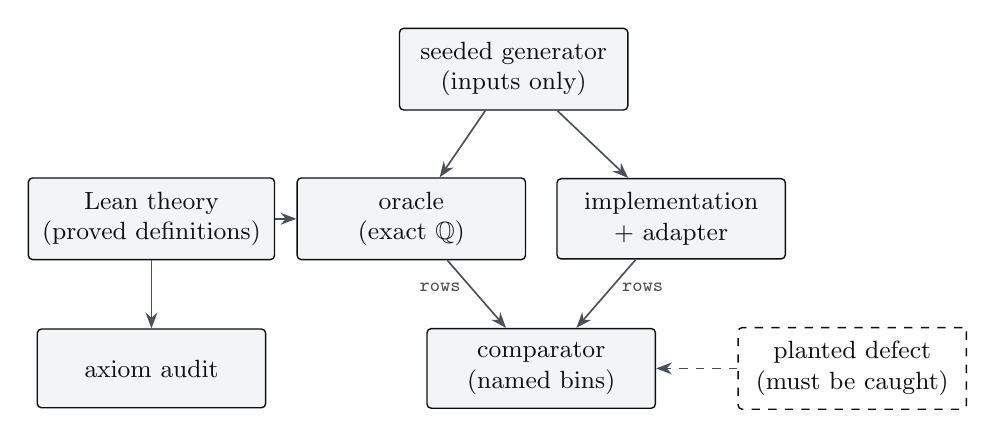
\begin{tikzpicture}[
  box/.style={draw=Ink, line width=0.5pt, fill=Surface, text=Ink, rounded corners=1.5pt,
    align=center, font=\small, inner sep=5pt, minimum height=10mm, minimum width=29mm},
  arr/.style={-{Stealth[length=2mm]}, line width=0.6pt, draw=InkMuted},
  lab/.style={font=\ttfamily\scriptsize, text=InkMuted}]
\node[box] (gen) at (4.6,1.9) {seeded generator\\(inputs only)};
\node[box] (theory) at (0,0) {Lean theory\\(proved definitions)};
\node[box] (oracle) at (3.3,0) {oracle\\(exact $\mathbb{Q}$)};
\node[box] (impl) at (6.6,0) {implementation\\+ adapter};
\node[box] (cmp) at (4.95,-1.9) {comparator\\(named bins)};
\node[box] (audit) at (0,-1.9) {axiom audit};
\node[box, dashed, fill=Background] (planted) at (8.9,-1.9) {planted defect\\(must be caught)};
\draw[arr] (gen) -- (oracle);
\draw[arr] (gen) -- (impl);
\draw[arr] (theory) -- (oracle);
\draw[arr] (theory) -- (audit);
\draw[arr] (oracle) -- node[left, lab, pos=0.4] {rows} (cmp);
\draw[arr] (impl) -- node[right, lab, pos=0.4] {rows} (cmp);
\draw[arr, dashed] (planted) -- (cmp);
\end{tikzpicture}
\caption{The measurement procedure. The generator never computes expected results;
those come only from the oracle.}
\label{fig:harness}
\end{figure}

The procedure follows \texttt{ledger-semantics} (\cref{fig:harness}). A seeded
generator writes case files containing inputs only. It favors the inputs where
implementations are known to have conventions: tied logits, words that are
themselves tokens, and merge tables with several splits of one string. A small
adapter per implementation runs the same cases and prints the oracle's row format.
The comparator places every case in exactly one named bin (agree, diverge, skipped
by either side, or missing), so nothing is dropped silently. Token rows are compared
as strings. Sampler rows require that a zero be matched by a zero and that nonzero
probabilities agree within $10^{-6}$, since llama.cpp stores logits in
\texttt{float32}. Each comparator is observed to fail: a planted defect, an adapter
that glues two tokens or one that inverts temperature, must be detected or the run
fails.

\paragraph{Tie divergences.} An implementation that keeps exactly $k$ tokens breaks
ties in its own order, which need not be the oracle's order by index. Every filter
treats tied tokens alike except for that choice, and tied tokens stay tied through
temperature and renormalization. Such an implementation must therefore agree with
the positional semantics up to a permutation of tied tokens. The harness checks
exactly this: the multiset of (logit, probability) pairs over the kept tokens must
equal that of the oracle's \texttt{q} rows. A divergence that fails this check is
reported as unexplained.

\begin{table}[t]
\centering\small
\caption{Measurements (\texttt{harness/run.sh 600}: four seeds of 600 cases each per
corpus). Lean 4.34.1, Mathlib v4.34.1, \texttt{tokenizers} 0.23.3, \texttt{tiktoken}
0.14.0, llama.cpp commit \texttt{a9d27ac} (2026-10-11).}
\label{tab:results}
\begin{tabularx}{\linewidth}{@{}>{\raggedright\arraybackslash}p{4.6cm}>{\raggedright\arraybackslash}X>{\raggedright\arraybackslash}X@{}}
\toprule
\qpth{Implementation} & \qpth{Compared against} & \qpth{Result}\\
\midrule
HF \texttt{tokenizers}, BPE, defaults & rule-rank BPE (\lean{bpe}) & 13{,}779 / 13{,}779 words identical\\
HF \texttt{tokenizers}, \lean{ignore_merges} & lookup, then rule-rank BPE & 13{,}779 / 13{,}779 identical\\
\texttt{tiktoken} & lookup, then concatenation-rank BPE & 13{,}779 / 13{,}779 identical\\
llama.cpp \lean{top_k}, \lean{top_p}, \lean{min_p}, \texttt{temp}, no ties & tie-keeping filters & 1{,}216 / 1{,}216 chains, $|\Delta p|\le5.1\times10^{-8}$\\
llama.cpp, with ties & tie-keeping, else positional & 939 + 245 / 1{,}184 chains; 0 unexplained\\
Planted defects (tokenizer, sampler) & --- & both detected\\
\bottomrule
\end{tabularx}
\end{table}

\Cref{tab:results} summarizes the results. Two findings came out of the
comparisons. First, \texttt{tiktoken} initially disagreed with the oracle's
concatenation-rank BPE on words that are themselves vocabulary tokens. The
disagreement was a convention, whole-word lookup. Following the
\texttt{ledger-semantics} rule that a divergence is either a defect in the
implementation or a convention the semantics has not yet recorded, we recorded it
as \lean{lookupFirst}, with its own theorems, after which agreement is exact.
Second, on the same random merge tables the two tokenizer libraries disagree with
each other on 439 of 13{,}779 words (3.2\%), and on 279 when Hugging Face uses
\lean{ignore_merges}. The oracle reproduces each library exactly, so every one of
these disagreements is predicted. \Cref{thm:bpeconv} states the condition under which
they cannot occur.

For sampling, llama.cpp agrees with the tie-keeping semantics on every tie-free
chain. On chains with ties, 245 of 1{,}184 diverge, and every one agrees with the
positional semantics up to a permutation of tied tokens. Some of these divergences
cascade: a tie cut by top-$k$ changes the renormalized masses that a later top-$p$
sees. A check that compared kept sets only after the fact would misclassify such
cases. Replaying the convention exactly classifies all of them.

% ===========================================================================
\section{Related work}

\paragraph{Formal methods for machine learning.} Most verification work on neural
networks proves properties of trained models, for example with SMT-based
methods~\cite{katz2017reluplex}. We verify the model-independent algorithms around
the model instead, and connect them to implementations through an oracle. The
denotational method follows Elliott~\cite{elliott2009denotational}. The use of a
proved semantics as a test oracle, the procedure of planted defects, and the
discipline of named skip bins follow \texttt{ledger-semantics}~\cite{ledgersemantics}.
Our category of finite stochastic maps is a special case of Fritz's Markov
categories~\cite{fritz2020markov}.

\paragraph{Tokenization.} Zouhar et al.\ give a formal analysis of BPE as an
optimization problem~\cite{zouhar2023bpe}. Gastaldi et al.\ treat tokenizers as
stochastic maps and study consistency of estimators~\cite{gastaldi2024foundations}.
Vieira et al.\ show how to turn token-level models into character-level
ones~\cite{vieira2024tokens}, which requires exactly the enumeration of
tokenizations we verify. Our no-compression theorem and the agreement criterion
between BPE conventions complement this work at the level of exact identities.

\paragraph{Decoding.} Top-$k$~\cite{fan2018hierarchical}, nucleus~\cite{holtzman2020curious}
and min-$p$~\cite{nguyen2025minp} sampling are usually specified by an algorithm over
sorted arrays, which leaves ties unspecified. \Cref{thm:topk} shows that this gap
cannot be closed by any symmetric rule. Speculative
sampling~\cite{leviathan2023speculative,chen2023speculative} is known to be lossless,
and its acceptance rate is the maximal-coupling bound~\cite{lindvall1992coupling}. Du et
al.\ characterize tightness measure-theoretically~\cite{du2023tight}. We give a
finite-depth statement and an explicit non-tight model.

\paragraph{Attention and inference systems.} Online softmax~\cite{milakov2018online}
underlies FlashAttention~\cite{dao2022flashattention} and its successors, and
KV caching is standard in serving systems~\cite{pope2023scaling,kwon2023vllm}. Our
contribution is the algebraic packaging, a commutative monoid with a free-monoid
homomorphism, and machine-checked proofs over arbitrary exponential characters.
Permutation equivariance of attention without positional encodings is
known~\cite{yun2020universal}.

\paragraph{Masked diffusion.} The time-independence of the optimal denoiser was
observed by Ou et al.~\cite{ou2025absorbing}, in the setting of
D3PM~\cite{austin2021d3pm}, MDLM~\cite{sahoo2024mdlm} and related
models~\cite{shi2024masked,nie2025llada}. We machine-check it, together with the
any-order chain rule and the inexactness of parallel unmasking.

% ===========================================================================
\section{Limitations}

Analysis on the reals enters only through exponential characters, and there is no
measure theory, so sampling and tightness are stated through finite quantities. The
oracle's temperature is restricted to $1/n$, which keeps softmax rational. The
theorems hold for every temperature, but the oracle cannot evaluate an irrational
softmax. Speculative decoding is proved for one drafted token. The sequence version
follows by induction and is not yet formalized. Nothing is proved about
floating-point arithmetic: implementations are compared with exact values within a
stated tolerance. A decision that lies exactly on a floating-point boundary could in
principle diverge, and none occurred in our runs. The diffusion theory covers
absorbing diffusion, not Gaussian diffusion. The chat protocol models tool calling in
its common request-and-result form, not any vendor's specification. The measurements
cover tokenizers and samplers; attention kernels, speculative decoders, chat
renderers and diffusion samplers are evaluated by the oracle but not yet compared
against implementations.

% ===========================================================================
\section{Conclusion}

The inference side of LLMs is small enough to be given a precise meaning and large
enough that its implementations disagree. A machine-checked semantics separates
what is meaning from what is convention. It proves which reorderings, cachings and
tilings are harmless, and it shows that some properties folklore expects, such as
symmetric exact top-$k$, compositional compressing tokenizers and unambiguous plain-text
templates, cannot exist. Connected to an exact oracle, the same definitions become
a test instrument. Every divergence it surfaces is either a defect in an
implementation or a convention that belongs in the semantics.

\paragraph{Availability.} The Lean development, oracle, harness, and recorded
measurement log accompany this paper.

\paragraph{Acknowledgments.} The structure of this work follows
\texttt{ledger-semantics} by John Wiegley. The formalization and harness were
developed with the assistance of an AI system (Claude, Anthropic).

% ===========================================================================
\begin{thebibliography}{99}\small

\bibitem{austin2021d3pm}
J.~Austin, D.~D. Johnson, J.~Ho, D.~Tarlow, and R.~van~den Berg.
\newblock Structured denoising diffusion models in discrete state-spaces.
\newblock In \emph{NeurIPS}, 2021.

\bibitem{chen2023speculative}
C.~Chen, S.~Borgeaud, G.~Irving, J.-B. Lespiau, L.~Sifre, and J.~Jumper.
\newblock Accelerating large language model decoding with speculative sampling.
\newblock arXiv:2302.01318, 2023.

\bibitem{dao2022flashattention}
T.~Dao, D.~Y. Fu, S.~Ermon, A.~Rudra, and C.~R{\'e}.
\newblock {FlashAttention}: Fast and memory-efficient exact attention with {IO}-awareness.
\newblock In \emph{NeurIPS}, 2022.

\bibitem{demoura2021lean4}
L.~de~Moura and S.~Ullrich.
\newblock The {Lean} 4 theorem prover and programming language.
\newblock In \emph{CADE-28}, 2021.

\bibitem{du2023tight}
L.~Du, L.~Torroba~Hennigen, T.~Pimentel, C.~Meister, J.~Eisner, and R.~Cotterell.
\newblock A measure-theoretic characterization of tight language models.
\newblock In \emph{ACL}, 2023.

\bibitem{elliott2009denotational}
C.~Elliott.
\newblock Denotational design with type class morphisms.
\newblock Technical Report 2009-01, LambdaPix, 2009.

\bibitem{fan2018hierarchical}
A.~Fan, M.~Lewis, and Y.~Dauphin.
\newblock Hierarchical neural story generation.
\newblock In \emph{ACL}, 2018.

\bibitem{fritz2020markov}
T.~Fritz.
\newblock A synthetic approach to {Markov} kernels, conditional independence and theorems on sufficient statistics.
\newblock \emph{Advances in Mathematics}, 370, 2020.

\bibitem{gastaldi2024foundations}
J.~L. Gastaldi, J.~Terilla, L.~Malagutti, B.~DuSell, T.~Vieira, and R.~Cotterell.
\newblock The foundations of tokenization: Statistical and computational concerns.
\newblock arXiv:2407.11606, 2024.

\bibitem{greshake2023injection}
K.~Greshake, S.~Abdelnabi, S.~Mishra, C.~Endres, T.~Holz, and M.~Fritz.
\newblock Not what you've signed up for: Compromising real-world {LLM}-integrated applications with indirect prompt injection.
\newblock In \emph{AISec}, 2023.

\bibitem{holtzman2020curious}
A.~Holtzman, J.~Buys, L.~Du, M.~Forbes, and Y.~Choi.
\newblock The curious case of neural text degeneration.
\newblock In \emph{ICLR}, 2020.

\bibitem{katz2017reluplex}
G.~Katz, C.~Barrett, D.~L. Dill, K.~Julian, and M.~J. Kochenderfer.
\newblock Reluplex: An efficient {SMT} solver for verifying deep neural networks.
\newblock In \emph{CAV}, 2017.

\bibitem{kwon2023vllm}
W.~Kwon, Z.~Li, S.~Zhuang, Y.~Sheng, L.~Zheng, C.~H. Yu, J.~E. Gonzalez, H.~Zhang, and I.~Stoica.
\newblock Efficient memory management for large language model serving with {PagedAttention}.
\newblock In \emph{SOSP}, 2023.

\bibitem{ledgersemantics}
J.~Wiegley.
\newblock ledger-semantics: Mathematical semantics of {Ledger}, the double-entry accounting tool.
\newblock \url{https://github.com/ledger/ledger-semantics}, 2026.

\bibitem{leviathan2023speculative}
Y.~Leviathan, M.~Kalman, and Y.~Matias.
\newblock Fast inference from transformers via speculative decoding.
\newblock In \emph{ICML}, 2023.

\bibitem{lindvall1992coupling}
T.~Lindvall.
\newblock \emph{Lectures on the Coupling Method}.
\newblock Wiley, 1992.

\bibitem{liu2023ring}
H.~Liu, M.~Zaharia, and P.~Abbeel.
\newblock Ring attention with blockwise transformers for near-infinite context.
\newblock arXiv:2310.01889, 2023.

\bibitem{mathlib2020}
The mathlib Community.
\newblock The {Lean} mathematical library.
\newblock In \emph{CPP}, 2020.

\bibitem{milakov2018online}
M.~Milakov and N.~Gimelshein.
\newblock Online normalizer calculation for softmax.
\newblock arXiv:1805.02867, 2018.

\bibitem{nguyen2025minp}
M.~N. Nguyen, A.~Baker, C.~Neo, A.~Roush, A.~Kirsch, and R.~Shwartz-Ziv.
\newblock Turning up the heat: Min-p sampling for creative and coherent {LLM} outputs.
\newblock In \emph{ICLR}, 2025.

\bibitem{nie2025llada}
S.~Nie, F.~Zhu, Z.~You, X.~Zhang, J.~Ou, J.~Hu, J.~Zhou, Y.~Lin, J.-R. Wen, and C.~Li.
\newblock Large language diffusion models.
\newblock arXiv:2502.09992, 2025.

\bibitem{ou2025absorbing}
J.~Ou, S.~Nie, K.~Xue, F.~Zhu, J.~Sun, Z.~Li, and C.~Li.
\newblock Your absorbing discrete diffusion secretly models the conditional distributions of clean data.
\newblock In \emph{ICLR}, 2025.

\bibitem{pope2023scaling}
R.~Pope, S.~Douglas, A.~Chowdhery, J.~Devlin, J.~Bradbury, J.~Heek, K.~Xiao, S.~Agrawal, and J.~Dean.
\newblock Efficiently scaling transformer inference.
\newblock In \emph{MLSys}, 2023.

\bibitem{rabe2021selfattention}
M.~N. Rabe and C.~Staats.
\newblock Self-attention does not need {$O(n^2)$} memory.
\newblock arXiv:2112.05682, 2021.

\bibitem{radford2019gpt2}
A.~Radford, J.~Wu, R.~Child, D.~Luan, D.~Amodei, and I.~Sutskever.
\newblock Language models are unsupervised multitask learners.
\newblock OpenAI technical report, 2019.

\bibitem{sahoo2024mdlm}
S.~S. Sahoo, M.~Arriola, Y.~Schiff, A.~Gokaslan, E.~Marroquin, J.~T. Chiu, A.~Rush, and V.~Kuleshov.
\newblock Simple and effective masked diffusion language models.
\newblock In \emph{NeurIPS}, 2024.

\bibitem{sennrich2016bpe}
R.~Sennrich, B.~Haddow, and A.~Birch.
\newblock Neural machine translation of rare words with subword units.
\newblock In \emph{ACL}, 2016.

\bibitem{shi2024masked}
J.~Shi, K.~Han, Z.~Wang, A.~Doucet, and M.~K. Titsias.
\newblock Simplified and generalized masked diffusion for discrete data.
\newblock In \emph{NeurIPS}, 2024.

\bibitem{vieira2024tokens}
T.~Vieira, B.~LeBrun, M.~Giulianelli, J.~L. Gastaldi, B.~DuSell, J.~Terilla, T.~J. O'Donnell, and R.~Cotterell.
\newblock From language models over tokens to language models over characters.
\newblock arXiv:2412.03719, 2024.

\bibitem{wolf2020transformers}
T.~Wolf et~al.
\newblock Transformers: State-of-the-art natural language processing.
\newblock In \emph{EMNLP: System Demonstrations}, 2020.

\bibitem{xiao2024sinks}
G.~Xiao, Y.~Tian, B.~Chen, S.~Han, and M.~Lewis.
\newblock Efficient streaming language models with attention sinks.
\newblock In \emph{ICLR}, 2024.

\bibitem{yun2020universal}
C.~Yun, S.~Bhojanapalli, A.~S. Rawat, S.~J. Reddi, and S.~Kumar.
\newblock Are transformers universal approximators of sequence-to-sequence functions?
\newblock In \emph{ICLR}, 2020.

\bibitem{zouhar2023bpe}
V.~Zouhar, C.~Meister, J.~L. Gastaldi, L.~Du, T.~Vieira, M.~Sachan, and R.~Cotterell.
\newblock A formal perspective on byte-pair encoding.
\newblock In \emph{Findings of ACL}, 2023.

\end{thebibliography}

\end{document}
"
% ---------------------------------------------------------------------------
\documentclass[10pt]{article}

\newif\ifqptdark
\qptdarkfalse   % print edition (light). \qptdarktrue gives the dark screen edition.
\ifdefined\qptdarkedition\qptdarktrue\fi  % or: xelatex "\def\qptdarkedition{}% !TeX program = xelatex
% ---------------------------------------------------------------------------
%  A Machine-Checked Semantics of LLM Inference
%  Daniel Arango Sohm, Universidad EAFIT
%
%  Typeset in the QPT visual design system:
%    * neutral-first: Ink on Background carries the document;
%    * paradigm colours are semantic only. This paper belongs to none of the
%      five paradigms, so no paradigm colour appears in its content; the
%      colours appear only in the QPT mark itself;
%    * no gradients;
%    * Space Grotesk for display, Inter for body text, IBM Plex Mono for
%      technical, numeric, label, code and proof-oriented content.
%
%  Compile with:  xelatex llm-semantics-qpt.tex   (twice, for references)
%  Dark screen edition: set \qptdarktrue below, or run
%    xelatex -jobname=llm-semantics-qpt-dark "\def\qptdarkedition{}% !TeX program = xelatex
% ---------------------------------------------------------------------------
%  A Machine-Checked Semantics of LLM Inference
%  Daniel Arango Sohm, Universidad EAFIT
%
%  Typeset in the QPT visual design system:
%    * neutral-first: Ink on Background carries the document;
%    * paradigm colours are semantic only. This paper belongs to none of the
%      five paradigms, so no paradigm colour appears in its content; the
%      colours appear only in the QPT mark itself;
%    * no gradients;
%    * Space Grotesk for display, Inter for body text, IBM Plex Mono for
%      technical, numeric, label, code and proof-oriented content.
%
%  Compile with:  xelatex llm-semantics-qpt.tex   (twice, for references)
%  Dark screen edition: set \qptdarktrue below, or run
%    xelatex -jobname=llm-semantics-qpt-dark "\def\qptdarkedition{}\input{llm-semantics-qpt}"
% ---------------------------------------------------------------------------
\documentclass[10pt]{article}

\newif\ifqptdark
\qptdarkfalse   % print edition (light). \qptdarktrue gives the dark screen edition.
\ifdefined\qptdarkedition\qptdarktrue\fi  % or: xelatex "\def\qptdarkedition{}\input{llm-semantics-qpt}"

\usepackage[a4paper,textwidth=15.4cm,textheight=23.6cm,top=3.0cm,headsep=0.9cm,footskip=1.2cm]{geometry}
\usepackage{amsmath,amssymb,amsthm,mathtools}
\usepackage{fontspec}
\usepackage{booktabs,tabularx,array}
\usepackage[protrusion=true,expansion=false]{microtype}
\usepackage[table]{xcolor}
\usepackage{graphicx}
\usepackage{fvextra}
\usepackage{enumitem}
\usepackage{caption}
\usepackage{titlesec}
\usepackage{fancyhdr}
\usepackage[most]{tcolorbox}
\usepackage{tikz}
\usetikzlibrary{arrows.meta}
\usepackage{hyperref}
\usepackage[nameinlink,capitalise]{cleveref}

% ---------------------------------------------------------------------------
%  Colour tokens
% ---------------------------------------------------------------------------
% Neutral foundation. Ink and Background invert between the two editions.
\ifqptdark
  \definecolor{Background}{HTML}{0B0C0E}
  \definecolor{Surface}{HTML}{16181B}
  \definecolor{Border}{HTML}{2B2E33}
  \definecolor{Ink}{HTML}{EDEEF0}
  \definecolor{InkMuted}{HTML}{A9AEB6}
  \definecolor{InkFaint}{HTML}{5A5F67}   % decoration only, never meaningful text
\else
  \definecolor{Background}{HTML}{FFFFFF}
  \definecolor{Surface}{HTML}{F3F4F5}
  \definecolor{Border}{HTML}{DADDE1}
  \definecolor{Ink}{HTML}{0E0F11}
  \definecolor{InkMuted}{HTML}{4B4F57}
  \definecolor{InkFaint}{HTML}{A3A7AE}   % decoration only, never meaningful text
\fi
% Paradigm colours: fixed in both editions, semantic only.
\definecolor{Quantum}{HTML}{5BAD1E}
\definecolor{Photonic}{HTML}{F0AB00}
\definecolor{Thermodynamic}{HTML}{E8690A}
\definecolor{Ternary}{HTML}{8A8A8A}
\definecolor{Bio}{HTML}{1AAB7C}

\ifqptdark\pagecolor{Background}\fi

% ---------------------------------------------------------------------------
%  Typography
% ---------------------------------------------------------------------------
\setmainfont{Inter}[
  Path=fonts/, Extension=.otf, Scale=0.94,
  UprightFont=*-Regular, ItalicFont=*-Italic,
  BoldFont=*-SemiBold, BoldItalicFont=*-SemiBoldItalic]
\setmonofont{IBMPlexMono}[
  Path=fonts/, Extension=.ttf, Scale=MatchLowercase,
  UprightFont=*-Regular, ItalicFont=*-Italic, BoldFont=*-SemiBold]
\newfontfamily\qptdisplay{SpaceGrotesk}[
  Path=fonts/, Extension=.otf, UprightFont=*-Medium, BoldFont=*-Bold]
\newfontfamily\qptdisplaylight{SpaceGrotesk}[
  Path=fonts/, Extension=.otf, UprightFont=*-Regular]
\newfontfamily\qptlabelfont{IBMPlexMono}[
  Path=fonts/, Extension=.ttf, Scale=MatchLowercase, UprightFont=*-Medium,
  LetterSpace=6]
\setsansfont{Inter}[
  Path=fonts/, Extension=.otf, Scale=0.94,
  UprightFont=*-Regular, ItalicFont=*-Italic,
  BoldFont=*-SemiBold, BoldItalicFont=*-SemiBoldItalic]
\linespread{1.16}
\setlength{\emergencystretch}{2.5em}
\AtBeginDocument{\raggedright\setlength{\parindent}{0pt}}
\setlength{\parindent}{0pt}
\setlength{\parskip}{0.55em}

% A label: IBM Plex Mono, upper case, tracked.
\newcommand{\qptlabel}[1]{{\qptlabelfont\footnotesize\MakeUppercase{#1}}}
% Technical names (Lean declarations, files) in IBM Plex Mono.
\newcommand{\lean}[1]{\texttt{\detokenize{#1}}}
\newcommand{\leanref}[1]{\par\smallskip\noindent
  {\ttfamily\footnotesize\upshape\raggedright\color{InkMuted}LEAN\enspace #1\par}}

% Ink is the normal colour everywhere, including floats, heads and footnotes.
\makeatletter
\AtBeginDocument{\color{Ink}\global\let\default@color\current@color}
\makeatother

% ---------------------------------------------------------------------------
%  Mathematical notation
% ---------------------------------------------------------------------------
\newcommand{\K}{\Bbbk}
\newcommand{\Dist}{\mathrm{Dist}}
\newcommand{\restr}[2]{#1|_{#2}}
\newcommand{\topk}{\mathrm{TopK}}
\newcommand{\topp}{\mathrm{TopP}}
\newcommand{\minp}{\mathrm{MinP}}
\newcommand{\sharpen}{\mathrm{sharpen}}
\newcommand{\abv}{\mathrm{above}}
\newcommand{\tv}{\mathrm{tv}}
\newcommand{\dec}{\mathrm{dec}}
\newcommand{\enc}{\mathrm{enc}}
\newcommand{\softmax}{\mathrm{softmax}}
\newcommand{\attend}{\mathrm{attend}}
\newcommand{\Iv}[1]{[\![#1]\!]}
\newcommand{\Mask}{\bot}

% ---------------------------------------------------------------------------
%  Headings: section numbers as labels, titles in Space Grotesk
% ---------------------------------------------------------------------------
\makeatletter
\newcommand{\qptsecnum}[1]{{\qptlabelfont\small\color{InkMuted}\two@digits{#1}}}
\makeatother
\titleformat{\section}
  {\qptdisplay\fontsize{14.5}{18}\selectfont\color{Ink}}
  {\qptsecnum{\value{section}}}{0.9em}{}
\titleformat{name=\section,numberless}
  {\qptdisplay\fontsize{14.5}{18}\selectfont\color{Ink}}{}{0pt}{}
\titlespacing*{\section}{0pt}{1.9em}{0.7em}
\titleformat{\paragraph}[runin]
  {\qptdisplay\normalsize\color{Ink}}{}{0pt}{}
\titlespacing*{\paragraph}{0pt}{0.9em}{0.6em}

% ---------------------------------------------------------------------------
%  Statements
% ---------------------------------------------------------------------------
\newtheoremstyle{qpt}
  {0.9em}{0.9em}
  {\normalfont}{}
  {\qptlabelfont\footnotesize}{}
  {\newline}
  {\MakeUppercase{\thmname{#1}\thmnumber{~#2}}%
   \thmnote{\enspace{\qptdisplay\normalsize\color{Ink}#3}}}
\theoremstyle{qpt}
\newtheorem{theorem}{Theorem}
\newtheorem{proposition}[theorem]{Proposition}
\newtheorem{corollary}[theorem]{Corollary}
\newtheorem{lemma}[theorem]{Lemma}
\newtheorem{definition}[theorem]{Definition}
\newtheorem{remark}[theorem]{Remark}

% Proofs: a tracked label and a neutral end mark.
\makeatletter
\renewcommand{\qedsymbol}{{\color{InkMuted}\rule{0.5em}{0.5em}}}
\renewenvironment{proof}[1][Proof]{\par\pushQED{\qed}\normalfont\topsep0.5em\relax
  \trivlist\item[\hskip\labelsep\qptlabel{#1}\hspace{0.6em}]\ignorespaces}
  {\popQED\endtrivlist\@endpefalse}
\makeatother

% ---------------------------------------------------------------------------
%  Code: IBM Plex Mono on a neutral surface, with a hairline on the left
% ---------------------------------------------------------------------------
\tcbset{colupper=Ink, collower=Ink}
\tcbset{qptcode/.style={enhanced, colback=Surface, colframe=Surface,
  boxrule=0pt, arc=0pt, left=9pt, right=8pt, top=5pt, bottom=5pt,
  borderline west={1.2pt}{0pt}{InkFaint}, before skip=0.7em, after skip=0.7em}}
\newenvironment{leancode}
  {\VerbatimEnvironment\begin{tcolorbox}[qptcode]%
   \begin{Verbatim}[fontsize=\small,commandchars=\\\{\},
     codes={\catcode`\$=3\catcode`\^=7},formatcom=\color{Ink}]}
  {\end{Verbatim}\end{tcolorbox}}
\newenvironment{casecode}
  {\VerbatimEnvironment\begin{tcolorbox}[qptcode,before skip=0pt,after skip=0pt]%
   \begin{Verbatim}[fontsize=\footnotesize,formatcom=\color{Ink}]}
  {\end{Verbatim}\end{tcolorbox}}

% ---------------------------------------------------------------------------
%  Floats, tables, captions
% ---------------------------------------------------------------------------
\DeclareCaptionLabelFormat{qpt}{\qptlabel{#1~#2}}
\DeclareCaptionLabelSeparator{qptsep}{\quad}
\captionsetup{labelformat=qpt, labelsep=qptsep, font={small,color=Ink},
  justification=raggedright, singlelinecheck=false, skip=6pt}
\newcommand{\qpth}[1]{\qptlabel{#1}}
\arrayrulecolor{Ink}
\setlength{\heavyrulewidth}{0.7pt}
\setlength{\lightrulewidth}{0.35pt}
\renewcommand{\arraystretch}{1.22}

% ---------------------------------------------------------------------------
%  Running heads
% ---------------------------------------------------------------------------
\pagestyle{fancy}
\fancyhf{}
\fancyhead[L]{{\color{Ink}\qptlabel{Machine-checked semantics of LLM inference}}}
\fancyhead[R]{{\color{Ink}\qptlabel{D. Arango Sohm}}}
\fancyfoot[R]{{\ttfamily\small\color{InkMuted}\thepage}}
\renewcommand{\headrule}{{\color{Border}\hrule height 0.4pt}\vspace{-0.4pt}}
\renewcommand{\headrulewidth}{0.4pt}
\fancypagestyle{qptfirst}{\fancyhf{}%
  \fancyfoot[R]{{\ttfamily\small\color{InkMuted}\thepage}}%
  \renewcommand{\headrulewidth}{0pt}\renewcommand{\headrule}{}}

% ---------------------------------------------------------------------------
%  Links and references: neutral, never accent-coloured text
% ---------------------------------------------------------------------------
\hypersetup{colorlinks=true, linkcolor=Ink, citecolor=Ink, urlcolor=Ink,
  pdftitle={A Machine-Checked Semantics of LLM Inference},
  pdfauthor={Daniel Arango Sohm},
  pdfsubject={Formal semantics of large language model inference in Lean 4},
  pdfkeywords={Lean 4, Mathlib, formal verification, LLM inference, sampling,
    tokenization, attention, speculative decoding, diffusion language models}}
\makeatletter
\renewcommand{\@biblabel}[1]{{\ttfamily\color{InkMuted}[#1]}}
\renewcommand{\@cite}[2]{{\ttfamily[#1\if@tempswa, #2\fi]}}
\makeatother
\renewcommand{\refname}{References}

\setlist{itemsep=2pt, topsep=4pt}
\setlist[itemize]{label={\color{InkMuted}\textbullet}}

\begin{document}
\thispagestyle{qptfirst}

% ----------------------------------------------------------------- masthead
\noindent
\begin{minipage}[c]{0.5\linewidth}
  \includegraphics[height=1.9cm]{qpt-logo.png}
\end{minipage}%
\begin{minipage}[c]{0.5\linewidth}\raggedleft
  \qptlabel{Preprint}\\[2pt]
  \qptlabel{October 2026}
\end{minipage}

\vspace{1.6em}
{\color{Border}\rule{\linewidth}{0.4pt}}
\vspace{1.1em}

{\qptdisplay\fontsize{25}{29.5}\selectfont\color{Ink}
A Machine-Checked Semantics\\ of LLM Inference\par}
\vspace{0.55em}
{\qptdisplaylight\fontsize{13}{17}\selectfont\color{InkMuted}
Sampling, Attention, Tokenization, Chat, Decoding,\\ and Diffusion in Lean~4\par}

\vspace{1.5em}
{\large\bfseries Daniel Arango Sohm}\par
\vspace{0.15em}
{\color{InkMuted}Universidad EAFIT, Medellín, Colombia\\
Former member of the QPT team}\par

\vspace{1.4em}
% ----------------------------------------------------------------- abstract
\begin{tcolorbox}[enhanced, colback=Surface, colframe=Surface, colupper=Ink, boxrule=0pt,
  arc=0pt, left=12pt, right=12pt, top=9pt, bottom=10pt]
\qptlabel{Abstract}\par\vspace{0.35em}
{\small
The inference side of a large language model is a stack of small algorithms:
tokenizers, attention kernels, key--value caches, sampling filters, speculative
decoders, chat templates, and diffusion samplers. Each has several independent
implementations, and those implementations are usually tested against one another
rather than against a definition. We give these components a single mathematical
semantics, formalized in Lean~4 against Mathlib. The development comprises about
4{,}600 lines and 270 named theorems, and every declaration depends only on Lean's
three standard axioms. It proves the exact algebra of sampling filters, the
losslessness and optimality of speculative sampling, and the correctness of
key--value caching and of FlashAttention-style online softmax as a commutative
monoid. It proves that byte-pair encoding is lossless under every merge priority,
together with a decidable criterion for when the Hugging Face and \texttt{tiktoken}
conventions agree, a protocol checker for tool calls, and the time-independence of
the masked-diffusion denoiser. It also proves six negative results. No sampling
rule that treats tokens symmetrically can always keep exactly $k$ tokens. No
tokenizer that compresses can respect concatenation. Every chat template that writes
its role markers in the content alphabet is ambiguous. No transformer without
positional information can copy a fixed position. An autoregressive model need not
define a distribution over strings. Parallel unmasking in diffusion is inexact.
From the same definitions we build an executable oracle that evaluates test cases in
exact rational arithmetic, and a harness that measures implementations against it.
On 2{,}400 random merge tables, Hugging Face \texttt{tokenizers} and
\texttt{tiktoken} each agree with the oracle on all 13{,}779 test words, while
disagreeing with each other on 3.2\% of them. On 2{,}400 random sampler chains,
every divergence of llama.cpp from the tie-keeping semantics is accounted for
exactly by the positional semantics that the impossibility theorem forces.
\par}
\end{tcolorbox}

\vspace{0.3em}
\noindent\qptlabel{Keywords}\enspace{\small Lean~4 · Mathlib · formal verification ·
LLM inference · sampling · tokenization · attention · speculative decoding ·
diffusion language models}

\vspace{0.4em}
{\color{Border}\rule{\linewidth}{0.4pt}}

% ===========================================================================
\section{Introduction}

A deployed language model is a function from parameters and a context to a
distribution over tokens. Turning that distribution into text requires more
machinery. A tokenizer maps strings to token sequences. Attention kernels compute
the model's reads over a cached context. A chain of sampling filters reshapes the
next-token distribution. A speculative decoder may verify drafted tokens, a chat
template linearizes a conversation, and a diffusion sampler may unmask several
positions at once. Each of these components exists in many implementations, such as
Hugging Face \texttt{transformers} and \texttt{tokenizers}~\cite{wolf2020transformers},
\texttt{tiktoken}, vLLM~\cite{kwon2023vllm}, and llama.cpp. Their tests mostly
compare one implementation with another, or with remembered behavior.

This paper follows a different discipline, \emph{denotational design}~\cite{elliott2009denotational}.
One first says precisely what a thing means, then requires every operation to
preserve that meaning, and lets the implementation be whatever the equations force
it to be. The approach is that of \texttt{ledger-semantics}~\cite{ledgersemantics},
which formalizes double-entry accounting in Lean and uses the result as a test oracle
for the C++ Ledger program. We apply it to LLM inference. A sampling filter means
conditioning a distribution on a set. A KV-cached decoder means causal attention over
the whole prefix. A FlashAttention kernel means a softmax-weighted average. A chat
template means an injective encoding of a transcript. The theorems state when an
implementation preserves that meaning, and several of them state that no
implementation can.

\paragraph{Contributions.}
\begin{itemize}[leftmargin=*,itemsep=2pt]
\item A Lean~4 formalization against Mathlib~\cite{mathlib2020,demoura2021lean4}
  of sampling, speculative decoding, softmax and attention, tokenization, chat
  transcripts, autoregressive decoding, and masked diffusion
  (\cref{sec:foundations,sec:sampling,sec:spec,sec:attention,sec:tokenization,sec:chat,sec:decoding,sec:diffusion}).
  All definitions are stated over an arbitrary linearly ordered field, so one proof
  covers the real numbers of the literature and the exact rationals of the oracle.
\item Positive results in a common framework. They include the algebra of
  sampling filters, the optimality of speculative sampling, an online-softmax
  commutative monoid, a generic correctness theorem for BPE with a decidable
  agreement criterion between the two conventions in use, a protocol checker for
  tool calls, and the any-order chain rule for masked diffusion.
\item Six negative results that explain design constraints visible across
  implementations (\cref{sec:negative}).
\item An executable oracle that evaluates case files under the proved
  definitions in exact arithmetic, and a measurement of Hugging Face
  \texttt{tokenizers}, \texttt{tiktoken}, and llama.cpp against it (\cref{sec:oracle,sec:measure}).
\end{itemize}

Several of the positive results are known: losslessness of speculative
sampling~\cite{leviathan2023speculative,chen2023speculative}, correctness of online
softmax~\cite{milakov2018online,dao2022flashattention}, time-independence of the
absorbing-diffusion posterior~\cite{ou2025absorbing}, and the role of permutation
equivariance~\cite{yun2020universal}. Our contribution for these is a machine-checked
statement in one framework, connected to an oracle. To our knowledge the
following are not stated elsewhere in the form given here: the impossibility of
symmetric exact top-$k$ and nucleus selection, the no-compression theorem for
homomorphic tokenizers, the ambiguity of every in-band chat template, and the
decidable agreement criterion between merge-rule and concatenation-rank BPE.

% ===========================================================================
\section{Method and trust base}\label{sec:method}

The development is a Lean~4 library (Lean 4.34.1, Mathlib v4.34.1) of eleven
theory modules and two executable modules (\cref{tab:modules}). It is built with
warnings promoted to errors, so an unproved theorem (\lean{sorry}) fails the build.
A separate audit program walks every declaration in the library, 853 in all, and
fails unless each depends only on propositional extensionality, the axiom of choice,
and quotient soundness. The audit has been observed to fail: a planted proof by
\lean{native_decide}, which introduces an auxiliary axiom trusting compiled code, is
rejected. The warnings-as-errors build alone does not catch it. Concrete
counterexamples are therefore proved by \lean{decide}, whose certificate the kernel
checks by evaluation.

\begin{table}[t]
\centering\small
\caption{Modules of the development. Lines and named theorems and lemmas per module.}
\label{tab:modules}
\begin{tabularx}{\linewidth}{@{}l>{\raggedright\arraybackslash}X>{\ttfamily}r>{\ttfamily}r@{}}
\toprule
\qpth{Module} & \qpth{Content} & \qpth{Lines} & \qpth{Thms} \\
\midrule
\lean{Dist} & finite distributions, conditioning, total variation, $\mathsf{FinStoch}$ & 383 & 34\\
\lean{Sampling} & top-$k$, top-$p$, min-$p$, temperature, ties, inverse CDF & 732 & 46\\
\lean{Counterexamples} & kernel-checked failures of sampler laws & 52 & 4\\
\lean{Speculative} & speculative sampling, couplings & 194 & 17\\
\lean{Softmax} & exponential characters, masking, temperature & 220 & 23\\
\lean{Attention} & equivariance, causality, KV cache, online softmax & 573 & 38\\
\lean{Real} & $\exp$ as a character; textbook restatements & 51 & 4\\
\lean{Tokenization} & free-monoid decoding, BPE conventions, enumeration & 860 & 49\\
\lean{Chat} & tool-call protocol, rendering & 440 & 21\\
\lean{Decoding} & mass conservation, tightness, greedy decoding & 245 & 15\\
\lean{Diffusion} & masked diffusion, posterior, chain rule & 379 & 18\\
\lean{Oracle}, \lean{Driver} & case parsing and exact evaluation & 465 & 1\\
\midrule
Total & & 4{,}594 & 270\\
\bottomrule
\end{tabularx}
\end{table}

\paragraph{Numbers.} Every probability lives in an arbitrary field $\K$ with a
compatible linear order (\lean{[Field K] [LinearOrder K] [IsStrictOrderedRing K]}).
The oracle instantiates $\K=\mathbb{Q}$, so its arithmetic is exact. The analytic
statements instantiate $\K=\mathbb{R}$. No measure theory is used. Sampling is made
precise through interval statements (\cref{thm:invcdf}), and tightness through
masses at finite depth (\cref{sec:decoding}).

% ===========================================================================
\section{Foundations}\label{sec:foundations}

\begin{definition}[Finite distribution]
For a finite type $\alpha$, $\Dist_\K(\alpha)$ is the type of functions
$p:\alpha\to\K$ with $p(a)\ge 0$ for all $a$ and $\sum_a p(a)=1$.
\leanref{\lean{Dist}}
\end{definition}

\begin{leancode}
structure Dist ($\K$ : Type u) [Field $\K$] [LinearOrder $\K$] [IsStrictOrderedRing $\K$]
    ($\alpha$ : Type v) [Fintype $\alpha$] where
  prob : $\alpha$ $\to$ $\K$
  nonneg : $\forall$ a, 0 $\le$ prob a
  sum_eq_one : $\sum$ a, prob a = 1
\end{leancode}

The single operation through which masks, filters and grammar constraints act is
conditioning. For $S\subseteq\alpha$ with $p(S)>0$, write
$\restr{p}{S}(a)=\Iv{a\in S}\,p(a)/p(S)$ (\lean{Dist.restrict}).

\begin{lemma}[Conditioning]\label{lem:restrict}
$\restr{(\restr{p}{S})}{T}=\restr{p}{S\cap T}$ whenever the masses involved are
positive. Moreover $\restr{p}{S}=\restr{p}{S'}$ whenever $S$ and $S'$ contain the same
outcomes of positive probability.
\leanref{\lean{restrict_restrict}, \lean{restrict_congr}}
\end{lemma}

The finite distribution monad (point masses and \lean{bind}) satisfies the monad
laws. Finite types and stochastic maps $\alpha\to\Dist_\K(\beta)$ form a category
$\mathsf{FinStoch}_\K$, given as an instance of Mathlib's \lean{Category} whose
composition is Kleisli composition (\lean{FinStoch.category}). Total variation is
$\tv(p,q)=\sum_a\max(0,p(a)-q(a))$. We prove
$\tv(p,q)=\tfrac12\sum_a|p(a)-q(a)|$, $\sum_a\min(p(a),q(a))=1-\tv(p,q)$, and
$\tv(p,q)=0\iff p=q$.

% ===========================================================================
\section{Sampling}\label{sec:sampling}

Let $V$ be a finite vocabulary and $p:V\to\K$. Write
$\abv_p(v)=\{u: p(v)<p(u)\}$ for the tokens strictly preferred to $v$. The three
standard filters keep the sets
\begin{gather*}
\topk_k(p)=\{v: |\abv_p(v)|<k\},\qquad
\minp_m(p)=\{v:\forall u,\; m\,p(u)\le p(v)\},\\
\topp_P(p)=\Bigl\{v: \textstyle\sum_{u\in\abv_p(v)}p(u)<P\Bigr\},
\end{gather*}
and the filtered distribution is the conditioning $\restr{p}{S}$ on the kept set
$S$. For distinct probabilities, $\topp_P$ is the usual rule ``sort in descending
order and keep the shortest prefix whose mass reaches $P$''. With ties, all three
keep every tied token. Temperature $1/n$ is
$\sharpen_n(p)(v)=p(v)^n/\sum_u p(u)^n$, which stays inside $\mathbb{Q}$. In
\cref{sec:attention} we show that it equals $\softmax(n\cdot z)$ when
$p=\softmax(z)$. Every kept set contains a most probable token, provided $k\ge1$,
$P>0$ and $m\le1$, so no filter can produce an empty distribution.

\begin{theorem}[Sampler algebra]\label{thm:algebra}
For $k,k'\ge1$, $m,m'\le1$ and $n\ge1$, and writing filters in the order they are
applied,
\begin{enumerate}[label=(\roman*),itemsep=1pt]
\item top-$k$ then top-$k'$ equals top-$\min(k,k')$;
\item min-$m$ then min-$m'$ equals min-$\max(m,m')$; in particular both filters are idempotent;
\item top-$k$ and min-$m$ commute;
\item top-$k$ and temperature $1/n$ commute.
\end{enumerate}
\leanref{\lean{topK_topK}, \lean{minP_minP}, \lean{topK_minP_comm}, \lean{topK_sharpen_comm}}
\end{theorem}

\begin{proof}[Proof sketch]
All three kept sets are \emph{upward closed}: if $v$ is kept and $p(v)<p(u)$, then
$u$ is kept. Conditioning on an upward-closed set $S$ leaves $\abv(v)$ unchanged for
$v\in S$ (\lean{above_restrict}), and min-$p$ is insensitive to conditioning on a set
that contains a maximizer (\lean{minP_restrict_iff}). Each identity then reduces,
through \cref{lem:restrict}, to an equality of kept sets. For (iv), $x\mapsto x^n$
is strictly increasing on $[0,\infty)$, and top-$k$ depends only on the order of the
scores (\lean{topKSet_congr}).
\end{proof}

The laws one might expect beyond \cref{thm:algebra} are false. With
$p_0=(\tfrac12,\tfrac3{10},\tfrac15)$, the kernel evaluates the following
(\lean{Counterexamples}).

\begin{proposition}[Failed laws]\label{prop:counter}
\leavevmode\vspace{-0.5\baselineskip}
\begin{enumerate}[label=(\roman*),itemsep=1pt]
\item Top-$p$ is not idempotent: one pass of $\topp_{3/5}$ gives token~1 the probability $\tfrac38$, and a second pass gives it~$0$.
\item Top-$p$ does not commute with top-$k$: top-$p$ then top-2 leaves token~1 at $\tfrac38$, while top-2 then top-$p$ removes it.
\item Top-$p$ does not commute with temperature $\tfrac12$: token~1 ends at $\tfrac9{34}$ in one order and at $0$ in the other.
\item Min-$p$ ($m=\tfrac12$) does not commute with temperature $\tfrac12$, with the same numbers.
\end{enumerate}
\end{proposition}

A sampler chain may therefore reorder top-$k$, min-$p$ and temperature only as
\cref{thm:algebra} allows, and may not move top-$p$ at all.

\paragraph{Ties.} Implementations differ on ties, and the difference is forced.
Call a selection rule $\mathrm{sel}:(V\to\K)\to\mathcal{P}(V)$ \emph{equivariant} if
$\mathrm{sel}(p\circ\sigma^{-1})=\sigma[\mathrm{sel}(p)]$ for every permutation
$\sigma$ of $V$, that is, if relabeling the tokens relabels the output.

\begin{theorem}[No symmetric exact top-$k$]\label{thm:topk}
Let $0<k<|V|$. No equivariant selection rule satisfies $|\mathrm{sel}(p)|=k$ for
every distribution $p$.
\leanref{\lean{no_equivariant_exact_topK}}
\end{theorem}
\begin{proof}
On the uniform distribution $u$ we have $u\circ\sigma^{-1}=u$ for every $\sigma$, so
$\mathrm{sel}(u)$ is invariant under all permutations. If it contains some $v$, then
for any $w$ the transposition $(v\,w)$ maps $v$ to $w$, so it contains $w$ too.
Hence $\mathrm{sel}(u)$ is either empty or all of $V$, and neither has $k$ elements.
\end{proof}

\begin{leancode}
theorem no_equivariant_exact_topK [DecidableEq V] \char123{}k : $\mathbb{N}$\char125{}
    (hk0 : 0 < k) (hkn : k < Fintype.card V)
    (sel : (V $\to$ $\K$) $\to$ Finset V) (hsel : Equivariant sel) :
    $\neg$ $\forall$ d : Dist $\K$ V, (sel d.prob).card = k
\end{leancode}

\begin{theorem}[No symmetric smallest nucleus]
Let $V$ be nonempty and $0<P\le1-1/|V|$. No equivariant rule returns, for every
distribution, a set of minimum cardinality among those of mass at least~$P$.
\leanref{\lean{no_equivariant_exact_nucleus}}
\end{theorem}

The tie-keeping filters are equivariant (\lean{topKSet_equivariant}). The other
option is to break ties by position. Define $u\prec_p v$ if $p(u)>p(v)$, or if
$p(u)=p(v)$ and $u<v$, and let the positional filters count predecessors under
$\prec_p$ instead of $\abv_p$ (\lean{Dist.topKPos}, \lean{Dist.topPPos}).

\begin{theorem}[Positional tie-breaking]
Positional top-$k$ keeps exactly $\min(k,|V|)$ tokens. If $p$ is injective, the
positional and tie-keeping filters coincide. For $0<k<|V|$, positional top-$k$ is
not equivariant.
\leanref{\lean{card_topKPosSet}, \lean{topKPosSet_eq_of_injective}, \lean{topPPosSet_eq_of_injective}, \lean{topKPosSet_not_equivariant}}
\end{theorem}

An implementation must therefore choose between keeping exactly $k$ tokens and
treating tokens symmetrically. Hugging Face \texttt{transformers} (read from the
source of version 5.19.0) keeps ties in top-$k$, since it removes only scores
strictly below the $k$-th largest, but breaks them by sort position in top-$p$.
llama.cpp breaks ties by position in both, as measured in \cref{sec:measure}.

\begin{theorem}[Inverse-CDF sampling]\label{thm:invcdf}
Let $F(i)=\sum_{j<i}p(j)$ on $V=\{0,\dots,n-1\}$ and let $\iota(u)$ be the least $i$
with $u<F(i+1)$. For $0\le u<1$, $\iota(u)=i\iff F(i)\le u<F(i+1)$, and
$F(i+1)-F(i)=p(i)$. A uniform $u$ therefore selects $i$ with probability $p(i)$.
\leanref{\lean{invCdf_eq_iff}, \lean{cdf_interval_length}}
\end{theorem}

% ===========================================================================
\section{Speculative decoding}\label{sec:spec}

A draft model proposes $x\sim q$. The target, with distribution $p$, accepts with
probability $a(x)=\min(1,p(x)/q(x))$, and on rejection a token is drawn from the
residual $r=(p-q)^+/\tv(p,q)$~\cite{leviathan2023speculative,chen2023speculative}.
We define the joint law of (draft, emitted token) exactly as the algorithm runs,
\[
\pi(x,y)=q(x)\bigl(a(x)\,\Iv{y=x}+(1-a(x))\,r(y)\bigr).
\]

\begin{theorem}[Speculative sampling]
\leavevmode\vspace{-0.5\baselineskip}
\begin{enumerate}[label=(\roman*),itemsep=1pt]
\item The draft has law $q$: $\sum_y\pi(x,y)=q(x)$.
\item \emph{Losslessness}: the emitted token has law $p$: $\sum_x\pi(x,y)=p(y)$.
\item The acceptance probability is $\sum_x q(x)a(x)=1-\tv(p,q)$, and the emitted token equals the draft with the same probability.
\item \emph{Optimality}: every coupling $\gamma$ of $q$ and $p$ has $\sum_x\gamma(x,x)\le1-\tv(p,q)$.
\end{enumerate}
\leanref{\lean{specJoint_fst}, \lean{specJoint_snd}, \lean{accept_rate}, \lean{specJoint_diag}, \lean{coupling_le}, \lean{spec_optimal}}
\end{theorem}
\begin{proof}[Proof sketch]
Since $q(x)a(x)=\min(p(x),q(x))$, the total rejection probability is $\tv(p,q)$,
and a rejected draft is never re-emitted, because $r(x)=0$ whenever $q(x)>p(x)$. For (iv),
$\gamma(x,x)\le\min(q(x),p(x))$ by the marginal constraints. This is the classical
coupling inequality~\cite{lindvall1992coupling}.
\end{proof}

Because any lossless rule for verifying one drafted token is a coupling, (iv) shows
that speculative sampling has the highest acceptance rate any such rule can achieve.

% ===========================================================================
\section{Softmax and attention}\label{sec:attention}

\begin{definition}[Exponential character]
An \emph{exponential character} from an ordered additive group $G$ of scores into
$\K$ is a strictly increasing map $E:G\to\K$ with $E(a)>0$ and $E(a+b)=E(a)E(b)$.
For $z:\iota\to G$, $\softmax_E(z)_i=E(z_i)/\sum_jE(z_j)$.
\leanref{\lean{ExpChar}}
\end{definition}

$\exp:\mathbb{R}\to\mathbb{R}$ is a character (\lean{ExpChar.real}). So is
$z\mapsto2^z:\mathbb{Z}\to\mathbb{Q}$ (\lean{ExpChar.base2}), which the oracle uses
to evaluate softmax with no rounding. Every result in this section holds for every
character, and so for both.

\begin{theorem}[Softmax]\label{thm:softmax}
\leavevmode\vspace{-0.5\baselineskip}
\begin{enumerate}[label=(\roman*),itemsep=1pt]
\item $\softmax_E(z+c)=\softmax_E(z)$; this licenses subtracting the maximum logit.
\item $\softmax_E(z)_i<\softmax_E(z)_j\iff z_i<z_j$.
\item \emph{Masking is conditioning}: setting logits outside $S$ to $-\infty$ and taking softmax gives $\restr{\softmax_E(z)}{S}$.
\item For $G$ a field and $T>0$, $\topk_k(\softmax_E(z/T))=\topk_k(z)$.
\item $\softmax_E(n\cdot z)=\sharpen_n(\softmax_E(z))$.
\end{enumerate}
\leanref{\lean{softmax_add_const}, \lean{softmax_lt_iff}, \lean{softmaxOn_eq_restrict}, \lean{topK_temperature}, \lean{softmax_nsmul}}
\end{theorem}

\paragraph{One read.} $\attend(s,v)=\sum_j\softmax_E(s)_j\,v_j$ for scores $s$ and
values $v_j$ in a $\K$-module.

\begin{theorem}[Convexity]
For every linear functional $\varphi$ and constant $c$, if $\varphi(v_j)\le c$ for all
$j$ then $\varphi(\attend(s,v))\le c$. If every $v_j=m$, then $\attend(s,v)=m$ for
every $s$.
\leanref{\lean{attend_convex}, \lean{attend_const}}
\end{theorem}

The second statement says attention cannot abstain. Its weights always sum to one,
which is the property that motivates attention-sink tokens~\cite{xiao2024sinks}.

\paragraph{Permutation equivariance.} A map $f:(\iota\to X)\to(\iota\to Y)$ is
equivariant if $f(x\circ\sigma)=f(x)\circ\sigma$ for every permutation~$\sigma$.

\begin{theorem}[Equivariance]
Self-attention with any score function and no positional information is
equivariant. So is any block $y=x+\sum_h\mathrm{attn}_h(\mathrm{norm}\,x)$,
$\mathrm{out}=y+\mathrm{mlp}(\mathrm{norm}\,y)$, and any stack of such blocks.
\leanref{\lean{selfAttn_equivariant}, \lean{block_equivariant}, \lean{stack_equivariant}}
\end{theorem}

\begin{theorem}[Positional information is necessary]\label{thm:nofirst}
If $\iota$ has two distinct positions $i_0\ne i_1$ and $X$ has two distinct elements,
no equivariant $f:(\iota\to X)\to(\iota\to X)$ satisfies $f(x)_i=x_{i_0}$ for all $x$ and $i$.
\leanref{\lean{no_equivariant_first}}
\end{theorem}
\begin{proof}
Let $x_{i_0}=a$ and $x_i=b$ elsewhere, and let $\sigma=(i_0\,i_1)$. Then
$f(x\circ\sigma)_{i_0}=(x\circ\sigma)_{i_0}=b$, while equivariance gives
$f(x\circ\sigma)_{i_0}=f(x)_{i_1}=x_{i_0}=a$.
\end{proof}

Without positional encodings, then, no transformer can output the token at a fixed
position~\cite{yun2020universal}.

\paragraph{Causality and the KV cache.} Causal attention over a list maps position
$i$ to a read with the query of $x_i$ over the keys and values of $x_0,\dots,x_i$
(\lean{causalAttn}). The cached decoder \lean{kvDecode} appends one (key, value) pair
per step and reads the cache, recomputing nothing.

\begin{theorem}[Causality and KV caching]
Causal attention is causal: it preserves length, and its output on a prefix is the
prefix of its output. Causal maps are closed under composition and residual sums.
\emph{KV caching is exact}: $\mathrm{kvDecode}(xs)=\mathrm{causalAttn}(xs)$. For any
causal $f$, $f(xs\mathbin{+\!\!+}[x])=f(xs)\mathbin{+\!\!+}(\text{last entry})$.
\leanref{\lean{causalAttn_causal}, \lean{kvDecode_eq}, \lean{causal_comp}, \lean{causal_extend}}
\end{theorem}

\paragraph{Online softmax as a monoid.} FlashAttention~\cite{dao2022flashattention},
memory-efficient attention~\cite{rabe2021selfattention} and ring
attention~\cite{liu2023ring} reduce attention over blocks of keys using the online
normalizer of Milakov and Gimelshein~\cite{milakov2018online}. A partial state is a
triple $(m,\ell,o)$ of running maximum, normalizer and accumulator, and two states
merge by rescaling to the larger maximum:
\[
(m_1,\ell_1,o_1)\otimes(m_2,\ell_2,o_2)=
\bigl(m,\;\ell_1E(m_1-m)+\ell_2E(m_2-m),\;E(m_1-m)\,o_1+E(m_2-m)\,o_2\bigr),
\]
where $m=\max(m_1,m_2)$.

\begin{theorem}[Online softmax]
Adjoining an identity for the empty block, $\otimes$ is a commutative monoid. Let
$\mathrm{single}(s,v)=(s,1,v)$ and $\mathrm{fin}(m,\ell,o)=\ell^{-1}o$. For every
list of (score, value) pairs, $\mathrm{fin}\bigl(\prod_j\mathrm{single}(s_j,v_j)\bigr)
=\bigl(\sum_jE(s_j)\bigr)^{-1}\sum_jE(s_j)v_j$. The same holds for every partition
of the list into blocks and every order of the blocks. The running maximum of a
nonempty product is the maximum score, so every exponent the kernel evaluates is
$\le0$.
\leanref{\lean{Online}, \lean{finalize_ofList}, \lean{finalize_blocks}, \lean{ofList_perm}, \lean{ofList_max}}
\end{theorem}

The fold is the free-monoid homomorphism that \lean{single} induces
(\lean{ofList_eq_lift}). Correctness of tiling is then a homomorphism property
rather than a calculation.

% ===========================================================================
\section{Tokenization}\label{sec:tokenization}

A token $t$ spells a string $\mathrm{str}(t)$ over an alphabet $C$. Decoding is the
free-monoid homomorphism $\dec:T^*\to C^*$ that $\mathrm{str}$ induces
(\lean{decodeHom}).

\begin{theorem}[No compression]\label{thm:nocompress}
Suppose every token spells a nonempty string. If $\enc:C^*\to T^*$ satisfies
$\dec\circ\enc=\mathrm{id}$ and $\enc(a\,b)=\enc(a)\,\enc(b)$, then
$|\enc(s)|=|s|$ for every $s$, and every emitted token spells a single character.
Consequently, any tokenizer with $|\enc(s)|<|s|$ for some $s$ violates
$\enc(a\,b)=\enc(a)\,\enc(b)$ for some $a,b$.
\leanref{\lean{homomorphic_no_compression}, \lean{compressing_not_homomorphic}}
\end{theorem}
\begin{proof}[Proof sketch]
$\enc([c])$ is nonempty and decodes to $[c]$. Since each token decodes to at least
one character, it consists of exactly one token. Induct on $s$ using
$\enc(c\,s)=\enc([c])\,\enc(s)$.
\end{proof}

Tokenization therefore lies outside any compositional core, and boundary artifacts
such as the prompt-boundary problem are consequences of compression rather than
defects of one implementation. Tokenizations are not unique (\lean{decode_not_injective}).
\lean{tokenizations} enumerates every token sequence over a vocabulary that spells a
given string, and it is proved sound, complete and duplicate-free
(\lean{tokenizations_spec}, \lean{tokenizations_nodup}). The probability of a string
under a token-level model is the sum over this enumeration~\cite{vieira2024tokens,gastaldi2024foundations}.

\paragraph{BPE, generically.} Byte-pair
encoding~\cite{sennrich2016bpe,radford2019gpt2,zouhar2023bpe} repeatedly merges the
leftmost occurrence of the lowest-priority adjacent pair. We define it once, for an
arbitrary priority $f:T\times T\to\mathrm{Option}(\mathbb{N}\times T)$ that returns
a rank and a merged token (\lean{bpeWith}).

\begin{theorem}[Generic BPE]
Each step merges a pair of minimum rank, and every pair to its left has strictly
larger rank. The output contains no mergeable pair. BPE is idempotent. If $f$ is
\emph{sound}, meaning a merged token spells the concatenation of its parts, then BPE
is lossless.
\leanref{\lean{stepWith_spec}, \lean{bpeWith_normal}, \lean{bpeWith_idem}, \lean{bpeWith_decode}}
\end{theorem}

Two priorities are in use. Hugging Face \texttt{tokenizers} and the GPT-2 encoder
rank a pair by its merge \emph{rule} (\lean{rankOf}). \texttt{tiktoken} ranks a pair
by the rank of the \emph{token it would form} (\lean{concatRank}).

\begin{theorem}[Agreement of conventions]\label{thm:bpeconv}
Let $\mathcal{T}$ be a set of tokens closed under merging. If two priorities agree
on every pair from $\mathcal{T}$, their BPE outputs agree on every sequence over
$\mathcal{T}$. For a finite vocabulary this condition is decidable. Without it the
conventions differ: for the merges $(b,c),(a,b),(ab,c)$, the word $abc$ encodes as
$a\cdot bc$ under rule ranks and as $abc$ under concatenation ranks.
\leanref{\lean{bpeWith_congr}, \lean{hf_eq_tiktoken}, \lean{hf_ne_tiktoken}}
\end{theorem}

\texttt{tiktoken} also emits a word directly when the word is itself a vocabulary
token, and Hugging Face does the same with \lean{ignore_merges}. We record this
convention as \lean{lookupFirst}. It preserves losslessness (\lean{tikEncode_flatten})
and changes results (\lean{lookup_matters}). Finally, BPE does not find the shortest
tokenization (\lean{bpe_not_shortest}).

% ===========================================================================
\section{Chat transcripts}\label{sec:chat}

A transcript is a list of events: system, user and assistant messages,
$\mathrm{call}_i$ (a tool call with identifier $i$), and $\mathrm{result}_i$. Let
$c_i(\mathit{pre})$ and $r_i(\mathit{pre})$ count the calls and results with
identifier $i$, and let $\mathrm{NoPending}(\mathit{pre})$ mean $r_i=c_i$ for all
$i$. The protocol is stated per event, against the events before it.
\[
\mathrm{Allowed}(\mathit{pre},e)=
\begin{cases}
c_i(\mathit{pre})=0\wedge(\mathrm{NoPending}(\mathit{pre})\vee\mathrm{lastIsCall}(\mathit{pre})) & e=\mathrm{call}_i\\
c_i(\mathit{pre})=1\wedge r_i(\mathit{pre})=0 & e=\mathrm{result}_i\\
\mathrm{NoPending}(\mathit{pre}) & \text{otherwise.}
\end{cases}
\]
A transcript $es$ is \emph{valid} if every $es_k$ is allowed after $es_{<k}$.

\begin{theorem}[Protocol checker]
A single left-to-right pass with a state of (called, answered, last-was-call)
accepts exactly the valid transcripts. In a valid transcript every identifier is
called at most once and answered at most as often as it is called, and every result
is preceded by its call.
\leanref{\lean{check_iff_valid}, \lean{valid_counts}, \lean{result_has_call}}
\end{theorem}

Rendering with out-of-band markers, special symbols disjoint from content, is
invertible (\lean{parse_render}), and stays injective through any injective tokenizer
(\lean{render_encode_injective}). An \emph{in-band} template writes each event as
$\mathrm{open}(h)\,\mathit{body}\,\mathrm{close}$ with
$\mathrm{open}(h),\mathrm{close}\in C^*$.

\begin{theorem}[In-band ambiguity]\label{thm:inband}
For every choice of $\mathrm{open}$ and $\mathrm{close}$, in-band rendering is not
injective.
\leanref{\lean{inBand_not_injective}}
\end{theorem}
\begin{proof}
The single user message with body $\mathrm{close}\cdot\mathrm{open}(\mathrm{assistant})$
and the pair (empty user message, empty assistant message) both render to
$\mathrm{open}(\mathrm{user})\,\mathrm{close}\,\mathrm{open}(\mathrm{assistant})\,\mathrm{close}$.
\end{proof}

Role separation exists only at the token level, and only while user text cannot
produce a special token. This is the formal content behind the use of reserved tokens
as a defense against prompt injection~\cite{greshake2023injection}.

% ===========================================================================
\section{Autoregressive decoding}\label{sec:decoding}

A model assigns each prefix a distribution $m(\mathit{pre})\in\Dist_\K(V\cup\{\mathrm{eos}\})$.
Let $\mathrm{alive}_n$ be the probability of having generated $n$ tokens without
stopping, and $\mathrm{stopped}_n$ the probability of having stopped within~$n$.

\begin{theorem}[Mass conservation and tightness]
$\mathrm{stopped}_n+\mathrm{alive}_n=1$ for every $n$ and every starting prefix. If
every prefix stops with probability at least $\varepsilon$, then
$\mathrm{alive}_n\le(1-\varepsilon)^n$.
\leanref{\lean{mass_conservation}, \lean{alive_le_of_stop}}
\end{theorem}

\begin{theorem}[A non-tight model]\label{thm:leaky}
For the model that stops after $L$ tokens with probability $1/(L+2)^2$,
$\mathrm{alive}_n=\frac{n+2}{2(n+1)}$, so $\mathrm{stopped}_n<\frac12$ for every $n$.
\leanref{\lean{leaky_aliveMass}, \lean{stopped_lt_half}}
\end{theorem}

This model never places half of its probability on finite strings, so an
autoregressive model need not define a distribution over strings, the phenomenon
studied as tightness by Du et al.~\cite{du2023tight}.

\begin{theorem}[Greedy is not MAP]
There is a two-step model whose strictly most probable first token begins only
sequences of probability $\tfrac3{10}$, while another sequence has probability $\tfrac25$.
\leanref{\lean{greedy_not_map}}
\end{theorem}

Greedy decoding therefore does not find the most probable sequence, under any
tie-breaking.

% ===========================================================================
\section{Masked diffusion}\label{sec:diffusion}

Masked (absorbing) diffusion~\cite{austin2021d3pm,sahoo2024mdlm,shi2024masked,nie2025llada}
replaces each token, independently, with a mask symbol $\Mask$. The forward kernel
at keep rate $\alpha$ sends $v$ to $v$ with probability $\alpha$ and to $\Mask$ with
probability $1-\alpha$, and fixes $\Mask$.

\begin{theorem}[Forward process]
$\alpha\mapsto\mathrm{mask}_\alpha$ is a monoid homomorphism from the multiplicative
interval $[0,1]$ into the endomorphisms of $V\cup\{\Mask\}$ in $\mathsf{FinStoch}_\K$,
given as a Mathlib \lean{MonoidHom}. The sequence-level forward probability is
$q_\alpha(y\mid x)=\Iv{x\models y}\,(1-\alpha)^{\#\Mask(y)}\alpha^{n-\#\Mask(y)}$,
where $x\models y$ means $y$ agrees with $x$ wherever it is unmasked.
\leanref{\lean{forward}, \lean{maskProb_comp}, \lean{qSeq_closed}}
\end{theorem}

\begin{theorem}[Time-independent denoiser]\label{thm:timeindep}
For every data distribution $p$, every masked sequence $y$ and every $0<\alpha<1$,
\[
\frac{p(x)\,q_\alpha(y\mid x)}{\sum_{x'}p(x')\,q_\alpha(y\mid x')}
=\frac{\Iv{x\models y}\,p(x)}{\sum_{x'}\Iv{x'\models y}\,p(x')}.
\]
\leanref{\lean{posterior_time_independent}}
\end{theorem}

The optimal denoiser is therefore the data distribution conditioned on the unmasked
tokens, whatever the noise level, as observed by Ou et al.~\cite{ou2025absorbing}. The
factor that depends on $\alpha$ depends only on the mask pattern of $y$, and it
cancels. The closed-form reverse step used by samplers is the Bayes posterior of
the forward process (\lean{reverse_bayes}).

\begin{theorem}[Any-order chain rule]
Let $o_1,\dots,o_n$ enumerate the positions, and let $c_k$ be the exact conditional
probability that position $o_k$ holds $x_{o_k}$ given $x$ on $o_1,\dots,o_{k-1}$, with
$0/0=0$. Then $p(x)=\prod_kc_k$, and $c_k$ is the marginal of the posterior of
\cref{thm:timeindep} at $o_k$.
\leanref{\lean{chain_rule_fin}, \lean{posterior_marginal}}
\end{theorem}

Unmasking one position at a time with the exact denoiser therefore samples the data
distribution exactly, in every order.

\begin{proposition}[Parallel unmasking is inexact]
For the distribution uniform on $\{(0,1),(1,0)\}$, the product of the two exact
posterior marginals from the fully masked sequence gives $(1,1)$ the probability
$\tfrac14$, but $p(1,1)=0$.
\leanref{\lean{parallel_decoding_inexact}}
\end{proposition}

% ===========================================================================
\section{The negative results together}\label{sec:negative}

The six impossibility theorems share a shape. Each says that a property folklore
expects of a component is inconsistent with that component's purpose, and so each
explains a design constraint found in mature implementations.

\begin{enumerate}[label=(\arabic*),itemsep=2pt]
\item \emph{Symmetric exact top-$k$ does not exist} (\cref{thm:topk}). Every sampler must document its tie convention.
\item \emph{Compressing tokenizers are not compositional} (\cref{thm:nocompress}). Tokenization cannot be done piecewise, and prompt boundaries matter.
\item \emph{In-band chat templates are ambiguous} (\cref{thm:inband}). Roles require out-of-band special tokens.
\item \emph{Order requires positional information} (\cref{thm:nofirst}). Positional encodings are necessary, not an optimization.
\item \emph{Autoregressive models need not be tight} (\cref{thm:leaky}). Sequence-level probabilities need a stopping guarantee.
\item \emph{Parallel unmasking is inexact} (\cref{sec:diffusion}). Multi-token diffusion steps trade fidelity for speed.
\end{enumerate}

% ===========================================================================
\section{The oracle}\label{sec:oracle}

The oracle (\lean{LLM/Oracle.lean}, \lean{LLM/Driver.lean}) reads case files and
prints rows computed by the proved definitions over $\mathbb{Q}$. It runs under the
Lean interpreter (\texttt{lake env lean --run LLM/Driver.lean FILE}), so what
executes is a direct reading of the checked definitions. Inputs are validated at
run time, for example that probabilities are nonnegative and sum to one. The checks
are decidable propositions whose proofs construct the values the theorems speak
about.

\begin{figure}[t]
\begin{minipage}[t]{0.43\linewidth}
\begin{casecode}
@sample top-p is not idempotent
probs 1/2 3/10 1/5
top-p 3/5
emit
top-p 3/5
\end{casecode}
\end{minipage}\hfill
\begin{minipage}[t]{0.53\linewidth}
\begin{casecode}
-- top-p is not idempotent
p|0|5/8   p|1|3/8   p|2|0
q|0|5/8   q|1|3/8   q|2|0
p|0|1     p|1|0     p|2|0
q|0|1     q|1|0     q|2|0
\end{casecode}
\end{minipage}
\caption{A case file and the oracle's output, with rows placed side by side here.
Rows \texttt{p} use the tie-keeping filters and rows \texttt{q} the positional ones.
Every number is an exact rational.}
\label{fig:oracle}
\end{figure}

There are six case kinds. \texttt{@sample} runs a filter chain from probabilities,
weights, or integer logits under the base-2 softmax, and prints both tie
semantics (\cref{fig:oracle}). \texttt{@speculative} prints the acceptance rate,
total variation, per-token acceptance, residual, and emitted law. \texttt{@bpe}
prints the tokens under rule ranks, under rule ranks with whole-word lookup, and
under \texttt{tiktoken}'s convention, the number of tokenizations, and whether the
hypotheses of \cref{thm:bpeconv} hold. \texttt{@chat} prints validity with the first
offending event, and completeness. \texttt{@attention} prints softmax weights and
outputs, also through the online-softmax monoid over blocks. \texttt{@diffusion}
prints the evidence, posterior, and posterior marginals. A rejected case prints a
single \texttt{!!~ERROR} line.

% ===========================================================================
\section{Measuring implementations}\label{sec:measure}

\begin{figure}[t]
\centering
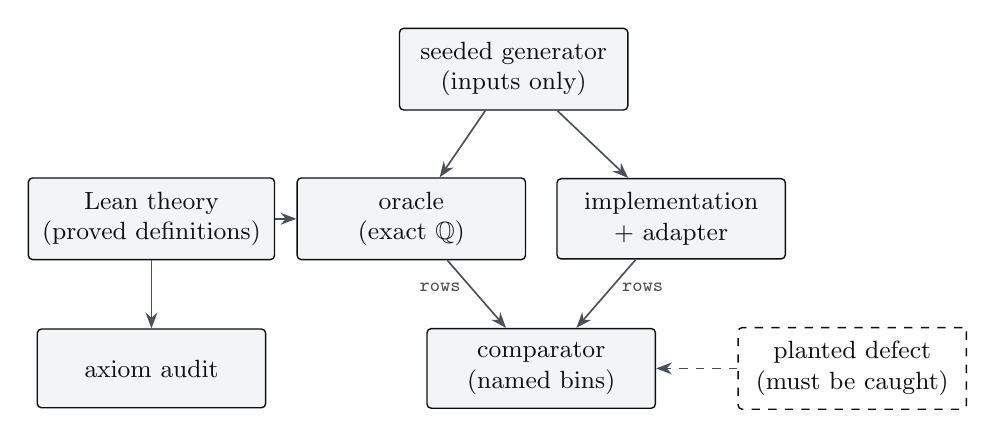
\begin{tikzpicture}[
  box/.style={draw=Ink, line width=0.5pt, fill=Surface, text=Ink, rounded corners=1.5pt,
    align=center, font=\small, inner sep=5pt, minimum height=10mm, minimum width=29mm},
  arr/.style={-{Stealth[length=2mm]}, line width=0.6pt, draw=InkMuted},
  lab/.style={font=\ttfamily\scriptsize, text=InkMuted}]
\node[box] (gen) at (4.6,1.9) {seeded generator\\(inputs only)};
\node[box] (theory) at (0,0) {Lean theory\\(proved definitions)};
\node[box] (oracle) at (3.3,0) {oracle\\(exact $\mathbb{Q}$)};
\node[box] (impl) at (6.6,0) {implementation\\+ adapter};
\node[box] (cmp) at (4.95,-1.9) {comparator\\(named bins)};
\node[box] (audit) at (0,-1.9) {axiom audit};
\node[box, dashed, fill=Background] (planted) at (8.9,-1.9) {planted defect\\(must be caught)};
\draw[arr] (gen) -- (oracle);
\draw[arr] (gen) -- (impl);
\draw[arr] (theory) -- (oracle);
\draw[arr] (theory) -- (audit);
\draw[arr] (oracle) -- node[left, lab, pos=0.4] {rows} (cmp);
\draw[arr] (impl) -- node[right, lab, pos=0.4] {rows} (cmp);
\draw[arr, dashed] (planted) -- (cmp);
\end{tikzpicture}
\caption{The measurement procedure. The generator never computes expected results;
those come only from the oracle.}
\label{fig:harness}
\end{figure}

The procedure follows \texttt{ledger-semantics} (\cref{fig:harness}). A seeded
generator writes case files containing inputs only. It favors the inputs where
implementations are known to have conventions: tied logits, words that are
themselves tokens, and merge tables with several splits of one string. A small
adapter per implementation runs the same cases and prints the oracle's row format.
The comparator places every case in exactly one named bin (agree, diverge, skipped
by either side, or missing), so nothing is dropped silently. Token rows are compared
as strings. Sampler rows require that a zero be matched by a zero and that nonzero
probabilities agree within $10^{-6}$, since llama.cpp stores logits in
\texttt{float32}. Each comparator is observed to fail: a planted defect, an adapter
that glues two tokens or one that inverts temperature, must be detected or the run
fails.

\paragraph{Tie divergences.} An implementation that keeps exactly $k$ tokens breaks
ties in its own order, which need not be the oracle's order by index. Every filter
treats tied tokens alike except for that choice, and tied tokens stay tied through
temperature and renormalization. Such an implementation must therefore agree with
the positional semantics up to a permutation of tied tokens. The harness checks
exactly this: the multiset of (logit, probability) pairs over the kept tokens must
equal that of the oracle's \texttt{q} rows. A divergence that fails this check is
reported as unexplained.

\begin{table}[t]
\centering\small
\caption{Measurements (\texttt{harness/run.sh 600}: four seeds of 600 cases each per
corpus). Lean 4.34.1, Mathlib v4.34.1, \texttt{tokenizers} 0.23.3, \texttt{tiktoken}
0.14.0, llama.cpp commit \texttt{a9d27ac} (2026-10-11).}
\label{tab:results}
\begin{tabularx}{\linewidth}{@{}>{\raggedright\arraybackslash}p{4.6cm}>{\raggedright\arraybackslash}X>{\raggedright\arraybackslash}X@{}}
\toprule
\qpth{Implementation} & \qpth{Compared against} & \qpth{Result}\\
\midrule
HF \texttt{tokenizers}, BPE, defaults & rule-rank BPE (\lean{bpe}) & 13{,}779 / 13{,}779 words identical\\
HF \texttt{tokenizers}, \lean{ignore_merges} & lookup, then rule-rank BPE & 13{,}779 / 13{,}779 identical\\
\texttt{tiktoken} & lookup, then concatenation-rank BPE & 13{,}779 / 13{,}779 identical\\
llama.cpp \lean{top_k}, \lean{top_p}, \lean{min_p}, \texttt{temp}, no ties & tie-keeping filters & 1{,}216 / 1{,}216 chains, $|\Delta p|\le5.1\times10^{-8}$\\
llama.cpp, with ties & tie-keeping, else positional & 939 + 245 / 1{,}184 chains; 0 unexplained\\
Planted defects (tokenizer, sampler) & --- & both detected\\
\bottomrule
\end{tabularx}
\end{table}

\Cref{tab:results} summarizes the results. Two findings came out of the
comparisons. First, \texttt{tiktoken} initially disagreed with the oracle's
concatenation-rank BPE on words that are themselves vocabulary tokens. The
disagreement was a convention, whole-word lookup. Following the
\texttt{ledger-semantics} rule that a divergence is either a defect in the
implementation or a convention the semantics has not yet recorded, we recorded it
as \lean{lookupFirst}, with its own theorems, after which agreement is exact.
Second, on the same random merge tables the two tokenizer libraries disagree with
each other on 439 of 13{,}779 words (3.2\%), and on 279 when Hugging Face uses
\lean{ignore_merges}. The oracle reproduces each library exactly, so every one of
these disagreements is predicted. \Cref{thm:bpeconv} states the condition under which
they cannot occur.

For sampling, llama.cpp agrees with the tie-keeping semantics on every tie-free
chain. On chains with ties, 245 of 1{,}184 diverge, and every one agrees with the
positional semantics up to a permutation of tied tokens. Some of these divergences
cascade: a tie cut by top-$k$ changes the renormalized masses that a later top-$p$
sees. A check that compared kept sets only after the fact would misclassify such
cases. Replaying the convention exactly classifies all of them.

% ===========================================================================
\section{Related work}

\paragraph{Formal methods for machine learning.} Most verification work on neural
networks proves properties of trained models, for example with SMT-based
methods~\cite{katz2017reluplex}. We verify the model-independent algorithms around
the model instead, and connect them to implementations through an oracle. The
denotational method follows Elliott~\cite{elliott2009denotational}. The use of a
proved semantics as a test oracle, the procedure of planted defects, and the
discipline of named skip bins follow \texttt{ledger-semantics}~\cite{ledgersemantics}.
Our category of finite stochastic maps is a special case of Fritz's Markov
categories~\cite{fritz2020markov}.

\paragraph{Tokenization.} Zouhar et al.\ give a formal analysis of BPE as an
optimization problem~\cite{zouhar2023bpe}. Gastaldi et al.\ treat tokenizers as
stochastic maps and study consistency of estimators~\cite{gastaldi2024foundations}.
Vieira et al.\ show how to turn token-level models into character-level
ones~\cite{vieira2024tokens}, which requires exactly the enumeration of
tokenizations we verify. Our no-compression theorem and the agreement criterion
between BPE conventions complement this work at the level of exact identities.

\paragraph{Decoding.} Top-$k$~\cite{fan2018hierarchical}, nucleus~\cite{holtzman2020curious}
and min-$p$~\cite{nguyen2025minp} sampling are usually specified by an algorithm over
sorted arrays, which leaves ties unspecified. \Cref{thm:topk} shows that this gap
cannot be closed by any symmetric rule. Speculative
sampling~\cite{leviathan2023speculative,chen2023speculative} is known to be lossless,
and its acceptance rate is the maximal-coupling bound~\cite{lindvall1992coupling}. Du et
al.\ characterize tightness measure-theoretically~\cite{du2023tight}. We give a
finite-depth statement and an explicit non-tight model.

\paragraph{Attention and inference systems.} Online softmax~\cite{milakov2018online}
underlies FlashAttention~\cite{dao2022flashattention} and its successors, and
KV caching is standard in serving systems~\cite{pope2023scaling,kwon2023vllm}. Our
contribution is the algebraic packaging, a commutative monoid with a free-monoid
homomorphism, and machine-checked proofs over arbitrary exponential characters.
Permutation equivariance of attention without positional encodings is
known~\cite{yun2020universal}.

\paragraph{Masked diffusion.} The time-independence of the optimal denoiser was
observed by Ou et al.~\cite{ou2025absorbing}, in the setting of
D3PM~\cite{austin2021d3pm}, MDLM~\cite{sahoo2024mdlm} and related
models~\cite{shi2024masked,nie2025llada}. We machine-check it, together with the
any-order chain rule and the inexactness of parallel unmasking.

% ===========================================================================
\section{Limitations}

Analysis on the reals enters only through exponential characters, and there is no
measure theory, so sampling and tightness are stated through finite quantities. The
oracle's temperature is restricted to $1/n$, which keeps softmax rational. The
theorems hold for every temperature, but the oracle cannot evaluate an irrational
softmax. Speculative decoding is proved for one drafted token. The sequence version
follows by induction and is not yet formalized. Nothing is proved about
floating-point arithmetic: implementations are compared with exact values within a
stated tolerance. A decision that lies exactly on a floating-point boundary could in
principle diverge, and none occurred in our runs. The diffusion theory covers
absorbing diffusion, not Gaussian diffusion. The chat protocol models tool calling in
its common request-and-result form, not any vendor's specification. The measurements
cover tokenizers and samplers; attention kernels, speculative decoders, chat
renderers and diffusion samplers are evaluated by the oracle but not yet compared
against implementations.

% ===========================================================================
\section{Conclusion}

The inference side of LLMs is small enough to be given a precise meaning and large
enough that its implementations disagree. A machine-checked semantics separates
what is meaning from what is convention. It proves which reorderings, cachings and
tilings are harmless, and it shows that some properties folklore expects, such as
symmetric exact top-$k$, compositional compressing tokenizers and unambiguous plain-text
templates, cannot exist. Connected to an exact oracle, the same definitions become
a test instrument. Every divergence it surfaces is either a defect in an
implementation or a convention that belongs in the semantics.

\paragraph{Availability.} The Lean development, oracle, harness, and recorded
measurement log accompany this paper.

\paragraph{Acknowledgments.} The structure of this work follows
\texttt{ledger-semantics} by John Wiegley. The formalization and harness were
developed with the assistance of an AI system (Claude, Anthropic).

% ===========================================================================
\begin{thebibliography}{99}\small

\bibitem{austin2021d3pm}
J.~Austin, D.~D. Johnson, J.~Ho, D.~Tarlow, and R.~van~den Berg.
\newblock Structured denoising diffusion models in discrete state-spaces.
\newblock In \emph{NeurIPS}, 2021.

\bibitem{chen2023speculative}
C.~Chen, S.~Borgeaud, G.~Irving, J.-B. Lespiau, L.~Sifre, and J.~Jumper.
\newblock Accelerating large language model decoding with speculative sampling.
\newblock arXiv:2302.01318, 2023.

\bibitem{dao2022flashattention}
T.~Dao, D.~Y. Fu, S.~Ermon, A.~Rudra, and C.~R{\'e}.
\newblock {FlashAttention}: Fast and memory-efficient exact attention with {IO}-awareness.
\newblock In \emph{NeurIPS}, 2022.

\bibitem{demoura2021lean4}
L.~de~Moura and S.~Ullrich.
\newblock The {Lean} 4 theorem prover and programming language.
\newblock In \emph{CADE-28}, 2021.

\bibitem{du2023tight}
L.~Du, L.~Torroba~Hennigen, T.~Pimentel, C.~Meister, J.~Eisner, and R.~Cotterell.
\newblock A measure-theoretic characterization of tight language models.
\newblock In \emph{ACL}, 2023.

\bibitem{elliott2009denotational}
C.~Elliott.
\newblock Denotational design with type class morphisms.
\newblock Technical Report 2009-01, LambdaPix, 2009.

\bibitem{fan2018hierarchical}
A.~Fan, M.~Lewis, and Y.~Dauphin.
\newblock Hierarchical neural story generation.
\newblock In \emph{ACL}, 2018.

\bibitem{fritz2020markov}
T.~Fritz.
\newblock A synthetic approach to {Markov} kernels, conditional independence and theorems on sufficient statistics.
\newblock \emph{Advances in Mathematics}, 370, 2020.

\bibitem{gastaldi2024foundations}
J.~L. Gastaldi, J.~Terilla, L.~Malagutti, B.~DuSell, T.~Vieira, and R.~Cotterell.
\newblock The foundations of tokenization: Statistical and computational concerns.
\newblock arXiv:2407.11606, 2024.

\bibitem{greshake2023injection}
K.~Greshake, S.~Abdelnabi, S.~Mishra, C.~Endres, T.~Holz, and M.~Fritz.
\newblock Not what you've signed up for: Compromising real-world {LLM}-integrated applications with indirect prompt injection.
\newblock In \emph{AISec}, 2023.

\bibitem{holtzman2020curious}
A.~Holtzman, J.~Buys, L.~Du, M.~Forbes, and Y.~Choi.
\newblock The curious case of neural text degeneration.
\newblock In \emph{ICLR}, 2020.

\bibitem{katz2017reluplex}
G.~Katz, C.~Barrett, D.~L. Dill, K.~Julian, and M.~J. Kochenderfer.
\newblock Reluplex: An efficient {SMT} solver for verifying deep neural networks.
\newblock In \emph{CAV}, 2017.

\bibitem{kwon2023vllm}
W.~Kwon, Z.~Li, S.~Zhuang, Y.~Sheng, L.~Zheng, C.~H. Yu, J.~E. Gonzalez, H.~Zhang, and I.~Stoica.
\newblock Efficient memory management for large language model serving with {PagedAttention}.
\newblock In \emph{SOSP}, 2023.

\bibitem{ledgersemantics}
J.~Wiegley.
\newblock ledger-semantics: Mathematical semantics of {Ledger}, the double-entry accounting tool.
\newblock \url{https://github.com/ledger/ledger-semantics}, 2026.

\bibitem{leviathan2023speculative}
Y.~Leviathan, M.~Kalman, and Y.~Matias.
\newblock Fast inference from transformers via speculative decoding.
\newblock In \emph{ICML}, 2023.

\bibitem{lindvall1992coupling}
T.~Lindvall.
\newblock \emph{Lectures on the Coupling Method}.
\newblock Wiley, 1992.

\bibitem{liu2023ring}
H.~Liu, M.~Zaharia, and P.~Abbeel.
\newblock Ring attention with blockwise transformers for near-infinite context.
\newblock arXiv:2310.01889, 2023.

\bibitem{mathlib2020}
The mathlib Community.
\newblock The {Lean} mathematical library.
\newblock In \emph{CPP}, 2020.

\bibitem{milakov2018online}
M.~Milakov and N.~Gimelshein.
\newblock Online normalizer calculation for softmax.
\newblock arXiv:1805.02867, 2018.

\bibitem{nguyen2025minp}
M.~N. Nguyen, A.~Baker, C.~Neo, A.~Roush, A.~Kirsch, and R.~Shwartz-Ziv.
\newblock Turning up the heat: Min-p sampling for creative and coherent {LLM} outputs.
\newblock In \emph{ICLR}, 2025.

\bibitem{nie2025llada}
S.~Nie, F.~Zhu, Z.~You, X.~Zhang, J.~Ou, J.~Hu, J.~Zhou, Y.~Lin, J.-R. Wen, and C.~Li.
\newblock Large language diffusion models.
\newblock arXiv:2502.09992, 2025.

\bibitem{ou2025absorbing}
J.~Ou, S.~Nie, K.~Xue, F.~Zhu, J.~Sun, Z.~Li, and C.~Li.
\newblock Your absorbing discrete diffusion secretly models the conditional distributions of clean data.
\newblock In \emph{ICLR}, 2025.

\bibitem{pope2023scaling}
R.~Pope, S.~Douglas, A.~Chowdhery, J.~Devlin, J.~Bradbury, J.~Heek, K.~Xiao, S.~Agrawal, and J.~Dean.
\newblock Efficiently scaling transformer inference.
\newblock In \emph{MLSys}, 2023.

\bibitem{rabe2021selfattention}
M.~N. Rabe and C.~Staats.
\newblock Self-attention does not need {$O(n^2)$} memory.
\newblock arXiv:2112.05682, 2021.

\bibitem{radford2019gpt2}
A.~Radford, J.~Wu, R.~Child, D.~Luan, D.~Amodei, and I.~Sutskever.
\newblock Language models are unsupervised multitask learners.
\newblock OpenAI technical report, 2019.

\bibitem{sahoo2024mdlm}
S.~S. Sahoo, M.~Arriola, Y.~Schiff, A.~Gokaslan, E.~Marroquin, J.~T. Chiu, A.~Rush, and V.~Kuleshov.
\newblock Simple and effective masked diffusion language models.
\newblock In \emph{NeurIPS}, 2024.

\bibitem{sennrich2016bpe}
R.~Sennrich, B.~Haddow, and A.~Birch.
\newblock Neural machine translation of rare words with subword units.
\newblock In \emph{ACL}, 2016.

\bibitem{shi2024masked}
J.~Shi, K.~Han, Z.~Wang, A.~Doucet, and M.~K. Titsias.
\newblock Simplified and generalized masked diffusion for discrete data.
\newblock In \emph{NeurIPS}, 2024.

\bibitem{vieira2024tokens}
T.~Vieira, B.~LeBrun, M.~Giulianelli, J.~L. Gastaldi, B.~DuSell, J.~Terilla, T.~J. O'Donnell, and R.~Cotterell.
\newblock From language models over tokens to language models over characters.
\newblock arXiv:2412.03719, 2024.

\bibitem{wolf2020transformers}
T.~Wolf et~al.
\newblock Transformers: State-of-the-art natural language processing.
\newblock In \emph{EMNLP: System Demonstrations}, 2020.

\bibitem{xiao2024sinks}
G.~Xiao, Y.~Tian, B.~Chen, S.~Han, and M.~Lewis.
\newblock Efficient streaming language models with attention sinks.
\newblock In \emph{ICLR}, 2024.

\bibitem{yun2020universal}
C.~Yun, S.~Bhojanapalli, A.~S. Rawat, S.~J. Reddi, and S.~Kumar.
\newblock Are transformers universal approximators of sequence-to-sequence functions?
\newblock In \emph{ICLR}, 2020.

\bibitem{zouhar2023bpe}
V.~Zouhar, C.~Meister, J.~L. Gastaldi, L.~Du, T.~Vieira, M.~Sachan, and R.~Cotterell.
\newblock A formal perspective on byte-pair encoding.
\newblock In \emph{Findings of ACL}, 2023.

\end{thebibliography}

\end{document}
"
% ---------------------------------------------------------------------------
\documentclass[10pt]{article}

\newif\ifqptdark
\qptdarkfalse   % print edition (light). \qptdarktrue gives the dark screen edition.
\ifdefined\qptdarkedition\qptdarktrue\fi  % or: xelatex "\def\qptdarkedition{}% !TeX program = xelatex
% ---------------------------------------------------------------------------
%  A Machine-Checked Semantics of LLM Inference
%  Daniel Arango Sohm, Universidad EAFIT
%
%  Typeset in the QPT visual design system:
%    * neutral-first: Ink on Background carries the document;
%    * paradigm colours are semantic only. This paper belongs to none of the
%      five paradigms, so no paradigm colour appears in its content; the
%      colours appear only in the QPT mark itself;
%    * no gradients;
%    * Space Grotesk for display, Inter for body text, IBM Plex Mono for
%      technical, numeric, label, code and proof-oriented content.
%
%  Compile with:  xelatex llm-semantics-qpt.tex   (twice, for references)
%  Dark screen edition: set \qptdarktrue below, or run
%    xelatex -jobname=llm-semantics-qpt-dark "\def\qptdarkedition{}\input{llm-semantics-qpt}"
% ---------------------------------------------------------------------------
\documentclass[10pt]{article}

\newif\ifqptdark
\qptdarkfalse   % print edition (light). \qptdarktrue gives the dark screen edition.
\ifdefined\qptdarkedition\qptdarktrue\fi  % or: xelatex "\def\qptdarkedition{}\input{llm-semantics-qpt}"

\usepackage[a4paper,textwidth=15.4cm,textheight=23.6cm,top=3.0cm,headsep=0.9cm,footskip=1.2cm]{geometry}
\usepackage{amsmath,amssymb,amsthm,mathtools}
\usepackage{fontspec}
\usepackage{booktabs,tabularx,array}
\usepackage[protrusion=true,expansion=false]{microtype}
\usepackage[table]{xcolor}
\usepackage{graphicx}
\usepackage{fvextra}
\usepackage{enumitem}
\usepackage{caption}
\usepackage{titlesec}
\usepackage{fancyhdr}
\usepackage[most]{tcolorbox}
\usepackage{tikz}
\usetikzlibrary{arrows.meta}
\usepackage{hyperref}
\usepackage[nameinlink,capitalise]{cleveref}

% ---------------------------------------------------------------------------
%  Colour tokens
% ---------------------------------------------------------------------------
% Neutral foundation. Ink and Background invert between the two editions.
\ifqptdark
  \definecolor{Background}{HTML}{0B0C0E}
  \definecolor{Surface}{HTML}{16181B}
  \definecolor{Border}{HTML}{2B2E33}
  \definecolor{Ink}{HTML}{EDEEF0}
  \definecolor{InkMuted}{HTML}{A9AEB6}
  \definecolor{InkFaint}{HTML}{5A5F67}   % decoration only, never meaningful text
\else
  \definecolor{Background}{HTML}{FFFFFF}
  \definecolor{Surface}{HTML}{F3F4F5}
  \definecolor{Border}{HTML}{DADDE1}
  \definecolor{Ink}{HTML}{0E0F11}
  \definecolor{InkMuted}{HTML}{4B4F57}
  \definecolor{InkFaint}{HTML}{A3A7AE}   % decoration only, never meaningful text
\fi
% Paradigm colours: fixed in both editions, semantic only.
\definecolor{Quantum}{HTML}{5BAD1E}
\definecolor{Photonic}{HTML}{F0AB00}
\definecolor{Thermodynamic}{HTML}{E8690A}
\definecolor{Ternary}{HTML}{8A8A8A}
\definecolor{Bio}{HTML}{1AAB7C}

\ifqptdark\pagecolor{Background}\fi

% ---------------------------------------------------------------------------
%  Typography
% ---------------------------------------------------------------------------
\setmainfont{Inter}[
  Path=fonts/, Extension=.otf, Scale=0.94,
  UprightFont=*-Regular, ItalicFont=*-Italic,
  BoldFont=*-SemiBold, BoldItalicFont=*-SemiBoldItalic]
\setmonofont{IBMPlexMono}[
  Path=fonts/, Extension=.ttf, Scale=MatchLowercase,
  UprightFont=*-Regular, ItalicFont=*-Italic, BoldFont=*-SemiBold]
\newfontfamily\qptdisplay{SpaceGrotesk}[
  Path=fonts/, Extension=.otf, UprightFont=*-Medium, BoldFont=*-Bold]
\newfontfamily\qptdisplaylight{SpaceGrotesk}[
  Path=fonts/, Extension=.otf, UprightFont=*-Regular]
\newfontfamily\qptlabelfont{IBMPlexMono}[
  Path=fonts/, Extension=.ttf, Scale=MatchLowercase, UprightFont=*-Medium,
  LetterSpace=6]
\setsansfont{Inter}[
  Path=fonts/, Extension=.otf, Scale=0.94,
  UprightFont=*-Regular, ItalicFont=*-Italic,
  BoldFont=*-SemiBold, BoldItalicFont=*-SemiBoldItalic]
\linespread{1.16}
\setlength{\emergencystretch}{2.5em}
\AtBeginDocument{\raggedright\setlength{\parindent}{0pt}}
\setlength{\parindent}{0pt}
\setlength{\parskip}{0.55em}

% A label: IBM Plex Mono, upper case, tracked.
\newcommand{\qptlabel}[1]{{\qptlabelfont\footnotesize\MakeUppercase{#1}}}
% Technical names (Lean declarations, files) in IBM Plex Mono.
\newcommand{\lean}[1]{\texttt{\detokenize{#1}}}
\newcommand{\leanref}[1]{\par\smallskip\noindent
  {\ttfamily\footnotesize\upshape\raggedright\color{InkMuted}LEAN\enspace #1\par}}

% Ink is the normal colour everywhere, including floats, heads and footnotes.
\makeatletter
\AtBeginDocument{\color{Ink}\global\let\default@color\current@color}
\makeatother

% ---------------------------------------------------------------------------
%  Mathematical notation
% ---------------------------------------------------------------------------
\newcommand{\K}{\Bbbk}
\newcommand{\Dist}{\mathrm{Dist}}
\newcommand{\restr}[2]{#1|_{#2}}
\newcommand{\topk}{\mathrm{TopK}}
\newcommand{\topp}{\mathrm{TopP}}
\newcommand{\minp}{\mathrm{MinP}}
\newcommand{\sharpen}{\mathrm{sharpen}}
\newcommand{\abv}{\mathrm{above}}
\newcommand{\tv}{\mathrm{tv}}
\newcommand{\dec}{\mathrm{dec}}
\newcommand{\enc}{\mathrm{enc}}
\newcommand{\softmax}{\mathrm{softmax}}
\newcommand{\attend}{\mathrm{attend}}
\newcommand{\Iv}[1]{[\![#1]\!]}
\newcommand{\Mask}{\bot}

% ---------------------------------------------------------------------------
%  Headings: section numbers as labels, titles in Space Grotesk
% ---------------------------------------------------------------------------
\makeatletter
\newcommand{\qptsecnum}[1]{{\qptlabelfont\small\color{InkMuted}\two@digits{#1}}}
\makeatother
\titleformat{\section}
  {\qptdisplay\fontsize{14.5}{18}\selectfont\color{Ink}}
  {\qptsecnum{\value{section}}}{0.9em}{}
\titleformat{name=\section,numberless}
  {\qptdisplay\fontsize{14.5}{18}\selectfont\color{Ink}}{}{0pt}{}
\titlespacing*{\section}{0pt}{1.9em}{0.7em}
\titleformat{\paragraph}[runin]
  {\qptdisplay\normalsize\color{Ink}}{}{0pt}{}
\titlespacing*{\paragraph}{0pt}{0.9em}{0.6em}

% ---------------------------------------------------------------------------
%  Statements
% ---------------------------------------------------------------------------
\newtheoremstyle{qpt}
  {0.9em}{0.9em}
  {\normalfont}{}
  {\qptlabelfont\footnotesize}{}
  {\newline}
  {\MakeUppercase{\thmname{#1}\thmnumber{~#2}}%
   \thmnote{\enspace{\qptdisplay\normalsize\color{Ink}#3}}}
\theoremstyle{qpt}
\newtheorem{theorem}{Theorem}
\newtheorem{proposition}[theorem]{Proposition}
\newtheorem{corollary}[theorem]{Corollary}
\newtheorem{lemma}[theorem]{Lemma}
\newtheorem{definition}[theorem]{Definition}
\newtheorem{remark}[theorem]{Remark}

% Proofs: a tracked label and a neutral end mark.
\makeatletter
\renewcommand{\qedsymbol}{{\color{InkMuted}\rule{0.5em}{0.5em}}}
\renewenvironment{proof}[1][Proof]{\par\pushQED{\qed}\normalfont\topsep0.5em\relax
  \trivlist\item[\hskip\labelsep\qptlabel{#1}\hspace{0.6em}]\ignorespaces}
  {\popQED\endtrivlist\@endpefalse}
\makeatother

% ---------------------------------------------------------------------------
%  Code: IBM Plex Mono on a neutral surface, with a hairline on the left
% ---------------------------------------------------------------------------
\tcbset{colupper=Ink, collower=Ink}
\tcbset{qptcode/.style={enhanced, colback=Surface, colframe=Surface,
  boxrule=0pt, arc=0pt, left=9pt, right=8pt, top=5pt, bottom=5pt,
  borderline west={1.2pt}{0pt}{InkFaint}, before skip=0.7em, after skip=0.7em}}
\newenvironment{leancode}
  {\VerbatimEnvironment\begin{tcolorbox}[qptcode]%
   \begin{Verbatim}[fontsize=\small,commandchars=\\\{\},
     codes={\catcode`\$=3\catcode`\^=7},formatcom=\color{Ink}]}
  {\end{Verbatim}\end{tcolorbox}}
\newenvironment{casecode}
  {\VerbatimEnvironment\begin{tcolorbox}[qptcode,before skip=0pt,after skip=0pt]%
   \begin{Verbatim}[fontsize=\footnotesize,formatcom=\color{Ink}]}
  {\end{Verbatim}\end{tcolorbox}}

% ---------------------------------------------------------------------------
%  Floats, tables, captions
% ---------------------------------------------------------------------------
\DeclareCaptionLabelFormat{qpt}{\qptlabel{#1~#2}}
\DeclareCaptionLabelSeparator{qptsep}{\quad}
\captionsetup{labelformat=qpt, labelsep=qptsep, font={small,color=Ink},
  justification=raggedright, singlelinecheck=false, skip=6pt}
\newcommand{\qpth}[1]{\qptlabel{#1}}
\arrayrulecolor{Ink}
\setlength{\heavyrulewidth}{0.7pt}
\setlength{\lightrulewidth}{0.35pt}
\renewcommand{\arraystretch}{1.22}

% ---------------------------------------------------------------------------
%  Running heads
% ---------------------------------------------------------------------------
\pagestyle{fancy}
\fancyhf{}
\fancyhead[L]{{\color{Ink}\qptlabel{Machine-checked semantics of LLM inference}}}
\fancyhead[R]{{\color{Ink}\qptlabel{D. Arango Sohm}}}
\fancyfoot[R]{{\ttfamily\small\color{InkMuted}\thepage}}
\renewcommand{\headrule}{{\color{Border}\hrule height 0.4pt}\vspace{-0.4pt}}
\renewcommand{\headrulewidth}{0.4pt}
\fancypagestyle{qptfirst}{\fancyhf{}%
  \fancyfoot[R]{{\ttfamily\small\color{InkMuted}\thepage}}%
  \renewcommand{\headrulewidth}{0pt}\renewcommand{\headrule}{}}

% ---------------------------------------------------------------------------
%  Links and references: neutral, never accent-coloured text
% ---------------------------------------------------------------------------
\hypersetup{colorlinks=true, linkcolor=Ink, citecolor=Ink, urlcolor=Ink,
  pdftitle={A Machine-Checked Semantics of LLM Inference},
  pdfauthor={Daniel Arango Sohm},
  pdfsubject={Formal semantics of large language model inference in Lean 4},
  pdfkeywords={Lean 4, Mathlib, formal verification, LLM inference, sampling,
    tokenization, attention, speculative decoding, diffusion language models}}
\makeatletter
\renewcommand{\@biblabel}[1]{{\ttfamily\color{InkMuted}[#1]}}
\renewcommand{\@cite}[2]{{\ttfamily[#1\if@tempswa, #2\fi]}}
\makeatother
\renewcommand{\refname}{References}

\setlist{itemsep=2pt, topsep=4pt}
\setlist[itemize]{label={\color{InkMuted}\textbullet}}

\begin{document}
\thispagestyle{qptfirst}

% ----------------------------------------------------------------- masthead
\noindent
\begin{minipage}[c]{0.5\linewidth}
  \includegraphics[height=1.9cm]{qpt-logo.png}
\end{minipage}%
\begin{minipage}[c]{0.5\linewidth}\raggedleft
  \qptlabel{Preprint}\\[2pt]
  \qptlabel{October 2026}
\end{minipage}

\vspace{1.6em}
{\color{Border}\rule{\linewidth}{0.4pt}}
\vspace{1.1em}

{\qptdisplay\fontsize{25}{29.5}\selectfont\color{Ink}
A Machine-Checked Semantics\\ of LLM Inference\par}
\vspace{0.55em}
{\qptdisplaylight\fontsize{13}{17}\selectfont\color{InkMuted}
Sampling, Attention, Tokenization, Chat, Decoding,\\ and Diffusion in Lean~4\par}

\vspace{1.5em}
{\large\bfseries Daniel Arango Sohm}\par
\vspace{0.15em}
{\color{InkMuted}Universidad EAFIT, Medellín, Colombia\\
Former member of the QPT team}\par

\vspace{1.4em}
% ----------------------------------------------------------------- abstract
\begin{tcolorbox}[enhanced, colback=Surface, colframe=Surface, colupper=Ink, boxrule=0pt,
  arc=0pt, left=12pt, right=12pt, top=9pt, bottom=10pt]
\qptlabel{Abstract}\par\vspace{0.35em}
{\small
The inference side of a large language model is a stack of small algorithms:
tokenizers, attention kernels, key--value caches, sampling filters, speculative
decoders, chat templates, and diffusion samplers. Each has several independent
implementations, and those implementations are usually tested against one another
rather than against a definition. We give these components a single mathematical
semantics, formalized in Lean~4 against Mathlib. The development comprises about
4{,}600 lines and 270 named theorems, and every declaration depends only on Lean's
three standard axioms. It proves the exact algebra of sampling filters, the
losslessness and optimality of speculative sampling, and the correctness of
key--value caching and of FlashAttention-style online softmax as a commutative
monoid. It proves that byte-pair encoding is lossless under every merge priority,
together with a decidable criterion for when the Hugging Face and \texttt{tiktoken}
conventions agree, a protocol checker for tool calls, and the time-independence of
the masked-diffusion denoiser. It also proves six negative results. No sampling
rule that treats tokens symmetrically can always keep exactly $k$ tokens. No
tokenizer that compresses can respect concatenation. Every chat template that writes
its role markers in the content alphabet is ambiguous. No transformer without
positional information can copy a fixed position. An autoregressive model need not
define a distribution over strings. Parallel unmasking in diffusion is inexact.
From the same definitions we build an executable oracle that evaluates test cases in
exact rational arithmetic, and a harness that measures implementations against it.
On 2{,}400 random merge tables, Hugging Face \texttt{tokenizers} and
\texttt{tiktoken} each agree with the oracle on all 13{,}779 test words, while
disagreeing with each other on 3.2\% of them. On 2{,}400 random sampler chains,
every divergence of llama.cpp from the tie-keeping semantics is accounted for
exactly by the positional semantics that the impossibility theorem forces.
\par}
\end{tcolorbox}

\vspace{0.3em}
\noindent\qptlabel{Keywords}\enspace{\small Lean~4 · Mathlib · formal verification ·
LLM inference · sampling · tokenization · attention · speculative decoding ·
diffusion language models}

\vspace{0.4em}
{\color{Border}\rule{\linewidth}{0.4pt}}

% ===========================================================================
\section{Introduction}

A deployed language model is a function from parameters and a context to a
distribution over tokens. Turning that distribution into text requires more
machinery. A tokenizer maps strings to token sequences. Attention kernels compute
the model's reads over a cached context. A chain of sampling filters reshapes the
next-token distribution. A speculative decoder may verify drafted tokens, a chat
template linearizes a conversation, and a diffusion sampler may unmask several
positions at once. Each of these components exists in many implementations, such as
Hugging Face \texttt{transformers} and \texttt{tokenizers}~\cite{wolf2020transformers},
\texttt{tiktoken}, vLLM~\cite{kwon2023vllm}, and llama.cpp. Their tests mostly
compare one implementation with another, or with remembered behavior.

This paper follows a different discipline, \emph{denotational design}~\cite{elliott2009denotational}.
One first says precisely what a thing means, then requires every operation to
preserve that meaning, and lets the implementation be whatever the equations force
it to be. The approach is that of \texttt{ledger-semantics}~\cite{ledgersemantics},
which formalizes double-entry accounting in Lean and uses the result as a test oracle
for the C++ Ledger program. We apply it to LLM inference. A sampling filter means
conditioning a distribution on a set. A KV-cached decoder means causal attention over
the whole prefix. A FlashAttention kernel means a softmax-weighted average. A chat
template means an injective encoding of a transcript. The theorems state when an
implementation preserves that meaning, and several of them state that no
implementation can.

\paragraph{Contributions.}
\begin{itemize}[leftmargin=*,itemsep=2pt]
\item A Lean~4 formalization against Mathlib~\cite{mathlib2020,demoura2021lean4}
  of sampling, speculative decoding, softmax and attention, tokenization, chat
  transcripts, autoregressive decoding, and masked diffusion
  (\cref{sec:foundations,sec:sampling,sec:spec,sec:attention,sec:tokenization,sec:chat,sec:decoding,sec:diffusion}).
  All definitions are stated over an arbitrary linearly ordered field, so one proof
  covers the real numbers of the literature and the exact rationals of the oracle.
\item Positive results in a common framework. They include the algebra of
  sampling filters, the optimality of speculative sampling, an online-softmax
  commutative monoid, a generic correctness theorem for BPE with a decidable
  agreement criterion between the two conventions in use, a protocol checker for
  tool calls, and the any-order chain rule for masked diffusion.
\item Six negative results that explain design constraints visible across
  implementations (\cref{sec:negative}).
\item An executable oracle that evaluates case files under the proved
  definitions in exact arithmetic, and a measurement of Hugging Face
  \texttt{tokenizers}, \texttt{tiktoken}, and llama.cpp against it (\cref{sec:oracle,sec:measure}).
\end{itemize}

Several of the positive results are known: losslessness of speculative
sampling~\cite{leviathan2023speculative,chen2023speculative}, correctness of online
softmax~\cite{milakov2018online,dao2022flashattention}, time-independence of the
absorbing-diffusion posterior~\cite{ou2025absorbing}, and the role of permutation
equivariance~\cite{yun2020universal}. Our contribution for these is a machine-checked
statement in one framework, connected to an oracle. To our knowledge the
following are not stated elsewhere in the form given here: the impossibility of
symmetric exact top-$k$ and nucleus selection, the no-compression theorem for
homomorphic tokenizers, the ambiguity of every in-band chat template, and the
decidable agreement criterion between merge-rule and concatenation-rank BPE.

% ===========================================================================
\section{Method and trust base}\label{sec:method}

The development is a Lean~4 library (Lean 4.34.1, Mathlib v4.34.1) of eleven
theory modules and two executable modules (\cref{tab:modules}). It is built with
warnings promoted to errors, so an unproved theorem (\lean{sorry}) fails the build.
A separate audit program walks every declaration in the library, 853 in all, and
fails unless each depends only on propositional extensionality, the axiom of choice,
and quotient soundness. The audit has been observed to fail: a planted proof by
\lean{native_decide}, which introduces an auxiliary axiom trusting compiled code, is
rejected. The warnings-as-errors build alone does not catch it. Concrete
counterexamples are therefore proved by \lean{decide}, whose certificate the kernel
checks by evaluation.

\begin{table}[t]
\centering\small
\caption{Modules of the development. Lines and named theorems and lemmas per module.}
\label{tab:modules}
\begin{tabularx}{\linewidth}{@{}l>{\raggedright\arraybackslash}X>{\ttfamily}r>{\ttfamily}r@{}}
\toprule
\qpth{Module} & \qpth{Content} & \qpth{Lines} & \qpth{Thms} \\
\midrule
\lean{Dist} & finite distributions, conditioning, total variation, $\mathsf{FinStoch}$ & 383 & 34\\
\lean{Sampling} & top-$k$, top-$p$, min-$p$, temperature, ties, inverse CDF & 732 & 46\\
\lean{Counterexamples} & kernel-checked failures of sampler laws & 52 & 4\\
\lean{Speculative} & speculative sampling, couplings & 194 & 17\\
\lean{Softmax} & exponential characters, masking, temperature & 220 & 23\\
\lean{Attention} & equivariance, causality, KV cache, online softmax & 573 & 38\\
\lean{Real} & $\exp$ as a character; textbook restatements & 51 & 4\\
\lean{Tokenization} & free-monoid decoding, BPE conventions, enumeration & 860 & 49\\
\lean{Chat} & tool-call protocol, rendering & 440 & 21\\
\lean{Decoding} & mass conservation, tightness, greedy decoding & 245 & 15\\
\lean{Diffusion} & masked diffusion, posterior, chain rule & 379 & 18\\
\lean{Oracle}, \lean{Driver} & case parsing and exact evaluation & 465 & 1\\
\midrule
Total & & 4{,}594 & 270\\
\bottomrule
\end{tabularx}
\end{table}

\paragraph{Numbers.} Every probability lives in an arbitrary field $\K$ with a
compatible linear order (\lean{[Field K] [LinearOrder K] [IsStrictOrderedRing K]}).
The oracle instantiates $\K=\mathbb{Q}$, so its arithmetic is exact. The analytic
statements instantiate $\K=\mathbb{R}$. No measure theory is used. Sampling is made
precise through interval statements (\cref{thm:invcdf}), and tightness through
masses at finite depth (\cref{sec:decoding}).

% ===========================================================================
\section{Foundations}\label{sec:foundations}

\begin{definition}[Finite distribution]
For a finite type $\alpha$, $\Dist_\K(\alpha)$ is the type of functions
$p:\alpha\to\K$ with $p(a)\ge 0$ for all $a$ and $\sum_a p(a)=1$.
\leanref{\lean{Dist}}
\end{definition}

\begin{leancode}
structure Dist ($\K$ : Type u) [Field $\K$] [LinearOrder $\K$] [IsStrictOrderedRing $\K$]
    ($\alpha$ : Type v) [Fintype $\alpha$] where
  prob : $\alpha$ $\to$ $\K$
  nonneg : $\forall$ a, 0 $\le$ prob a
  sum_eq_one : $\sum$ a, prob a = 1
\end{leancode}

The single operation through which masks, filters and grammar constraints act is
conditioning. For $S\subseteq\alpha$ with $p(S)>0$, write
$\restr{p}{S}(a)=\Iv{a\in S}\,p(a)/p(S)$ (\lean{Dist.restrict}).

\begin{lemma}[Conditioning]\label{lem:restrict}
$\restr{(\restr{p}{S})}{T}=\restr{p}{S\cap T}$ whenever the masses involved are
positive. Moreover $\restr{p}{S}=\restr{p}{S'}$ whenever $S$ and $S'$ contain the same
outcomes of positive probability.
\leanref{\lean{restrict_restrict}, \lean{restrict_congr}}
\end{lemma}

The finite distribution monad (point masses and \lean{bind}) satisfies the monad
laws. Finite types and stochastic maps $\alpha\to\Dist_\K(\beta)$ form a category
$\mathsf{FinStoch}_\K$, given as an instance of Mathlib's \lean{Category} whose
composition is Kleisli composition (\lean{FinStoch.category}). Total variation is
$\tv(p,q)=\sum_a\max(0,p(a)-q(a))$. We prove
$\tv(p,q)=\tfrac12\sum_a|p(a)-q(a)|$, $\sum_a\min(p(a),q(a))=1-\tv(p,q)$, and
$\tv(p,q)=0\iff p=q$.

% ===========================================================================
\section{Sampling}\label{sec:sampling}

Let $V$ be a finite vocabulary and $p:V\to\K$. Write
$\abv_p(v)=\{u: p(v)<p(u)\}$ for the tokens strictly preferred to $v$. The three
standard filters keep the sets
\begin{gather*}
\topk_k(p)=\{v: |\abv_p(v)|<k\},\qquad
\minp_m(p)=\{v:\forall u,\; m\,p(u)\le p(v)\},\\
\topp_P(p)=\Bigl\{v: \textstyle\sum_{u\in\abv_p(v)}p(u)<P\Bigr\},
\end{gather*}
and the filtered distribution is the conditioning $\restr{p}{S}$ on the kept set
$S$. For distinct probabilities, $\topp_P$ is the usual rule ``sort in descending
order and keep the shortest prefix whose mass reaches $P$''. With ties, all three
keep every tied token. Temperature $1/n$ is
$\sharpen_n(p)(v)=p(v)^n/\sum_u p(u)^n$, which stays inside $\mathbb{Q}$. In
\cref{sec:attention} we show that it equals $\softmax(n\cdot z)$ when
$p=\softmax(z)$. Every kept set contains a most probable token, provided $k\ge1$,
$P>0$ and $m\le1$, so no filter can produce an empty distribution.

\begin{theorem}[Sampler algebra]\label{thm:algebra}
For $k,k'\ge1$, $m,m'\le1$ and $n\ge1$, and writing filters in the order they are
applied,
\begin{enumerate}[label=(\roman*),itemsep=1pt]
\item top-$k$ then top-$k'$ equals top-$\min(k,k')$;
\item min-$m$ then min-$m'$ equals min-$\max(m,m')$; in particular both filters are idempotent;
\item top-$k$ and min-$m$ commute;
\item top-$k$ and temperature $1/n$ commute.
\end{enumerate}
\leanref{\lean{topK_topK}, \lean{minP_minP}, \lean{topK_minP_comm}, \lean{topK_sharpen_comm}}
\end{theorem}

\begin{proof}[Proof sketch]
All three kept sets are \emph{upward closed}: if $v$ is kept and $p(v)<p(u)$, then
$u$ is kept. Conditioning on an upward-closed set $S$ leaves $\abv(v)$ unchanged for
$v\in S$ (\lean{above_restrict}), and min-$p$ is insensitive to conditioning on a set
that contains a maximizer (\lean{minP_restrict_iff}). Each identity then reduces,
through \cref{lem:restrict}, to an equality of kept sets. For (iv), $x\mapsto x^n$
is strictly increasing on $[0,\infty)$, and top-$k$ depends only on the order of the
scores (\lean{topKSet_congr}).
\end{proof}

The laws one might expect beyond \cref{thm:algebra} are false. With
$p_0=(\tfrac12,\tfrac3{10},\tfrac15)$, the kernel evaluates the following
(\lean{Counterexamples}).

\begin{proposition}[Failed laws]\label{prop:counter}
\leavevmode\vspace{-0.5\baselineskip}
\begin{enumerate}[label=(\roman*),itemsep=1pt]
\item Top-$p$ is not idempotent: one pass of $\topp_{3/5}$ gives token~1 the probability $\tfrac38$, and a second pass gives it~$0$.
\item Top-$p$ does not commute with top-$k$: top-$p$ then top-2 leaves token~1 at $\tfrac38$, while top-2 then top-$p$ removes it.
\item Top-$p$ does not commute with temperature $\tfrac12$: token~1 ends at $\tfrac9{34}$ in one order and at $0$ in the other.
\item Min-$p$ ($m=\tfrac12$) does not commute with temperature $\tfrac12$, with the same numbers.
\end{enumerate}
\end{proposition}

A sampler chain may therefore reorder top-$k$, min-$p$ and temperature only as
\cref{thm:algebra} allows, and may not move top-$p$ at all.

\paragraph{Ties.} Implementations differ on ties, and the difference is forced.
Call a selection rule $\mathrm{sel}:(V\to\K)\to\mathcal{P}(V)$ \emph{equivariant} if
$\mathrm{sel}(p\circ\sigma^{-1})=\sigma[\mathrm{sel}(p)]$ for every permutation
$\sigma$ of $V$, that is, if relabeling the tokens relabels the output.

\begin{theorem}[No symmetric exact top-$k$]\label{thm:topk}
Let $0<k<|V|$. No equivariant selection rule satisfies $|\mathrm{sel}(p)|=k$ for
every distribution $p$.
\leanref{\lean{no_equivariant_exact_topK}}
\end{theorem}
\begin{proof}
On the uniform distribution $u$ we have $u\circ\sigma^{-1}=u$ for every $\sigma$, so
$\mathrm{sel}(u)$ is invariant under all permutations. If it contains some $v$, then
for any $w$ the transposition $(v\,w)$ maps $v$ to $w$, so it contains $w$ too.
Hence $\mathrm{sel}(u)$ is either empty or all of $V$, and neither has $k$ elements.
\end{proof}

\begin{leancode}
theorem no_equivariant_exact_topK [DecidableEq V] \char123{}k : $\mathbb{N}$\char125{}
    (hk0 : 0 < k) (hkn : k < Fintype.card V)
    (sel : (V $\to$ $\K$) $\to$ Finset V) (hsel : Equivariant sel) :
    $\neg$ $\forall$ d : Dist $\K$ V, (sel d.prob).card = k
\end{leancode}

\begin{theorem}[No symmetric smallest nucleus]
Let $V$ be nonempty and $0<P\le1-1/|V|$. No equivariant rule returns, for every
distribution, a set of minimum cardinality among those of mass at least~$P$.
\leanref{\lean{no_equivariant_exact_nucleus}}
\end{theorem}

The tie-keeping filters are equivariant (\lean{topKSet_equivariant}). The other
option is to break ties by position. Define $u\prec_p v$ if $p(u)>p(v)$, or if
$p(u)=p(v)$ and $u<v$, and let the positional filters count predecessors under
$\prec_p$ instead of $\abv_p$ (\lean{Dist.topKPos}, \lean{Dist.topPPos}).

\begin{theorem}[Positional tie-breaking]
Positional top-$k$ keeps exactly $\min(k,|V|)$ tokens. If $p$ is injective, the
positional and tie-keeping filters coincide. For $0<k<|V|$, positional top-$k$ is
not equivariant.
\leanref{\lean{card_topKPosSet}, \lean{topKPosSet_eq_of_injective}, \lean{topPPosSet_eq_of_injective}, \lean{topKPosSet_not_equivariant}}
\end{theorem}

An implementation must therefore choose between keeping exactly $k$ tokens and
treating tokens symmetrically. Hugging Face \texttt{transformers} (read from the
source of version 5.19.0) keeps ties in top-$k$, since it removes only scores
strictly below the $k$-th largest, but breaks them by sort position in top-$p$.
llama.cpp breaks ties by position in both, as measured in \cref{sec:measure}.

\begin{theorem}[Inverse-CDF sampling]\label{thm:invcdf}
Let $F(i)=\sum_{j<i}p(j)$ on $V=\{0,\dots,n-1\}$ and let $\iota(u)$ be the least $i$
with $u<F(i+1)$. For $0\le u<1$, $\iota(u)=i\iff F(i)\le u<F(i+1)$, and
$F(i+1)-F(i)=p(i)$. A uniform $u$ therefore selects $i$ with probability $p(i)$.
\leanref{\lean{invCdf_eq_iff}, \lean{cdf_interval_length}}
\end{theorem}

% ===========================================================================
\section{Speculative decoding}\label{sec:spec}

A draft model proposes $x\sim q$. The target, with distribution $p$, accepts with
probability $a(x)=\min(1,p(x)/q(x))$, and on rejection a token is drawn from the
residual $r=(p-q)^+/\tv(p,q)$~\cite{leviathan2023speculative,chen2023speculative}.
We define the joint law of (draft, emitted token) exactly as the algorithm runs,
\[
\pi(x,y)=q(x)\bigl(a(x)\,\Iv{y=x}+(1-a(x))\,r(y)\bigr).
\]

\begin{theorem}[Speculative sampling]
\leavevmode\vspace{-0.5\baselineskip}
\begin{enumerate}[label=(\roman*),itemsep=1pt]
\item The draft has law $q$: $\sum_y\pi(x,y)=q(x)$.
\item \emph{Losslessness}: the emitted token has law $p$: $\sum_x\pi(x,y)=p(y)$.
\item The acceptance probability is $\sum_x q(x)a(x)=1-\tv(p,q)$, and the emitted token equals the draft with the same probability.
\item \emph{Optimality}: every coupling $\gamma$ of $q$ and $p$ has $\sum_x\gamma(x,x)\le1-\tv(p,q)$.
\end{enumerate}
\leanref{\lean{specJoint_fst}, \lean{specJoint_snd}, \lean{accept_rate}, \lean{specJoint_diag}, \lean{coupling_le}, \lean{spec_optimal}}
\end{theorem}
\begin{proof}[Proof sketch]
Since $q(x)a(x)=\min(p(x),q(x))$, the total rejection probability is $\tv(p,q)$,
and a rejected draft is never re-emitted, because $r(x)=0$ whenever $q(x)>p(x)$. For (iv),
$\gamma(x,x)\le\min(q(x),p(x))$ by the marginal constraints. This is the classical
coupling inequality~\cite{lindvall1992coupling}.
\end{proof}

Because any lossless rule for verifying one drafted token is a coupling, (iv) shows
that speculative sampling has the highest acceptance rate any such rule can achieve.

% ===========================================================================
\section{Softmax and attention}\label{sec:attention}

\begin{definition}[Exponential character]
An \emph{exponential character} from an ordered additive group $G$ of scores into
$\K$ is a strictly increasing map $E:G\to\K$ with $E(a)>0$ and $E(a+b)=E(a)E(b)$.
For $z:\iota\to G$, $\softmax_E(z)_i=E(z_i)/\sum_jE(z_j)$.
\leanref{\lean{ExpChar}}
\end{definition}

$\exp:\mathbb{R}\to\mathbb{R}$ is a character (\lean{ExpChar.real}). So is
$z\mapsto2^z:\mathbb{Z}\to\mathbb{Q}$ (\lean{ExpChar.base2}), which the oracle uses
to evaluate softmax with no rounding. Every result in this section holds for every
character, and so for both.

\begin{theorem}[Softmax]\label{thm:softmax}
\leavevmode\vspace{-0.5\baselineskip}
\begin{enumerate}[label=(\roman*),itemsep=1pt]
\item $\softmax_E(z+c)=\softmax_E(z)$; this licenses subtracting the maximum logit.
\item $\softmax_E(z)_i<\softmax_E(z)_j\iff z_i<z_j$.
\item \emph{Masking is conditioning}: setting logits outside $S$ to $-\infty$ and taking softmax gives $\restr{\softmax_E(z)}{S}$.
\item For $G$ a field and $T>0$, $\topk_k(\softmax_E(z/T))=\topk_k(z)$.
\item $\softmax_E(n\cdot z)=\sharpen_n(\softmax_E(z))$.
\end{enumerate}
\leanref{\lean{softmax_add_const}, \lean{softmax_lt_iff}, \lean{softmaxOn_eq_restrict}, \lean{topK_temperature}, \lean{softmax_nsmul}}
\end{theorem}

\paragraph{One read.} $\attend(s,v)=\sum_j\softmax_E(s)_j\,v_j$ for scores $s$ and
values $v_j$ in a $\K$-module.

\begin{theorem}[Convexity]
For every linear functional $\varphi$ and constant $c$, if $\varphi(v_j)\le c$ for all
$j$ then $\varphi(\attend(s,v))\le c$. If every $v_j=m$, then $\attend(s,v)=m$ for
every $s$.
\leanref{\lean{attend_convex}, \lean{attend_const}}
\end{theorem}

The second statement says attention cannot abstain. Its weights always sum to one,
which is the property that motivates attention-sink tokens~\cite{xiao2024sinks}.

\paragraph{Permutation equivariance.} A map $f:(\iota\to X)\to(\iota\to Y)$ is
equivariant if $f(x\circ\sigma)=f(x)\circ\sigma$ for every permutation~$\sigma$.

\begin{theorem}[Equivariance]
Self-attention with any score function and no positional information is
equivariant. So is any block $y=x+\sum_h\mathrm{attn}_h(\mathrm{norm}\,x)$,
$\mathrm{out}=y+\mathrm{mlp}(\mathrm{norm}\,y)$, and any stack of such blocks.
\leanref{\lean{selfAttn_equivariant}, \lean{block_equivariant}, \lean{stack_equivariant}}
\end{theorem}

\begin{theorem}[Positional information is necessary]\label{thm:nofirst}
If $\iota$ has two distinct positions $i_0\ne i_1$ and $X$ has two distinct elements,
no equivariant $f:(\iota\to X)\to(\iota\to X)$ satisfies $f(x)_i=x_{i_0}$ for all $x$ and $i$.
\leanref{\lean{no_equivariant_first}}
\end{theorem}
\begin{proof}
Let $x_{i_0}=a$ and $x_i=b$ elsewhere, and let $\sigma=(i_0\,i_1)$. Then
$f(x\circ\sigma)_{i_0}=(x\circ\sigma)_{i_0}=b$, while equivariance gives
$f(x\circ\sigma)_{i_0}=f(x)_{i_1}=x_{i_0}=a$.
\end{proof}

Without positional encodings, then, no transformer can output the token at a fixed
position~\cite{yun2020universal}.

\paragraph{Causality and the KV cache.} Causal attention over a list maps position
$i$ to a read with the query of $x_i$ over the keys and values of $x_0,\dots,x_i$
(\lean{causalAttn}). The cached decoder \lean{kvDecode} appends one (key, value) pair
per step and reads the cache, recomputing nothing.

\begin{theorem}[Causality and KV caching]
Causal attention is causal: it preserves length, and its output on a prefix is the
prefix of its output. Causal maps are closed under composition and residual sums.
\emph{KV caching is exact}: $\mathrm{kvDecode}(xs)=\mathrm{causalAttn}(xs)$. For any
causal $f$, $f(xs\mathbin{+\!\!+}[x])=f(xs)\mathbin{+\!\!+}(\text{last entry})$.
\leanref{\lean{causalAttn_causal}, \lean{kvDecode_eq}, \lean{causal_comp}, \lean{causal_extend}}
\end{theorem}

\paragraph{Online softmax as a monoid.} FlashAttention~\cite{dao2022flashattention},
memory-efficient attention~\cite{rabe2021selfattention} and ring
attention~\cite{liu2023ring} reduce attention over blocks of keys using the online
normalizer of Milakov and Gimelshein~\cite{milakov2018online}. A partial state is a
triple $(m,\ell,o)$ of running maximum, normalizer and accumulator, and two states
merge by rescaling to the larger maximum:
\[
(m_1,\ell_1,o_1)\otimes(m_2,\ell_2,o_2)=
\bigl(m,\;\ell_1E(m_1-m)+\ell_2E(m_2-m),\;E(m_1-m)\,o_1+E(m_2-m)\,o_2\bigr),
\]
where $m=\max(m_1,m_2)$.

\begin{theorem}[Online softmax]
Adjoining an identity for the empty block, $\otimes$ is a commutative monoid. Let
$\mathrm{single}(s,v)=(s,1,v)$ and $\mathrm{fin}(m,\ell,o)=\ell^{-1}o$. For every
list of (score, value) pairs, $\mathrm{fin}\bigl(\prod_j\mathrm{single}(s_j,v_j)\bigr)
=\bigl(\sum_jE(s_j)\bigr)^{-1}\sum_jE(s_j)v_j$. The same holds for every partition
of the list into blocks and every order of the blocks. The running maximum of a
nonempty product is the maximum score, so every exponent the kernel evaluates is
$\le0$.
\leanref{\lean{Online}, \lean{finalize_ofList}, \lean{finalize_blocks}, \lean{ofList_perm}, \lean{ofList_max}}
\end{theorem}

The fold is the free-monoid homomorphism that \lean{single} induces
(\lean{ofList_eq_lift}). Correctness of tiling is then a homomorphism property
rather than a calculation.

% ===========================================================================
\section{Tokenization}\label{sec:tokenization}

A token $t$ spells a string $\mathrm{str}(t)$ over an alphabet $C$. Decoding is the
free-monoid homomorphism $\dec:T^*\to C^*$ that $\mathrm{str}$ induces
(\lean{decodeHom}).

\begin{theorem}[No compression]\label{thm:nocompress}
Suppose every token spells a nonempty string. If $\enc:C^*\to T^*$ satisfies
$\dec\circ\enc=\mathrm{id}$ and $\enc(a\,b)=\enc(a)\,\enc(b)$, then
$|\enc(s)|=|s|$ for every $s$, and every emitted token spells a single character.
Consequently, any tokenizer with $|\enc(s)|<|s|$ for some $s$ violates
$\enc(a\,b)=\enc(a)\,\enc(b)$ for some $a,b$.
\leanref{\lean{homomorphic_no_compression}, \lean{compressing_not_homomorphic}}
\end{theorem}
\begin{proof}[Proof sketch]
$\enc([c])$ is nonempty and decodes to $[c]$. Since each token decodes to at least
one character, it consists of exactly one token. Induct on $s$ using
$\enc(c\,s)=\enc([c])\,\enc(s)$.
\end{proof}

Tokenization therefore lies outside any compositional core, and boundary artifacts
such as the prompt-boundary problem are consequences of compression rather than
defects of one implementation. Tokenizations are not unique (\lean{decode_not_injective}).
\lean{tokenizations} enumerates every token sequence over a vocabulary that spells a
given string, and it is proved sound, complete and duplicate-free
(\lean{tokenizations_spec}, \lean{tokenizations_nodup}). The probability of a string
under a token-level model is the sum over this enumeration~\cite{vieira2024tokens,gastaldi2024foundations}.

\paragraph{BPE, generically.} Byte-pair
encoding~\cite{sennrich2016bpe,radford2019gpt2,zouhar2023bpe} repeatedly merges the
leftmost occurrence of the lowest-priority adjacent pair. We define it once, for an
arbitrary priority $f:T\times T\to\mathrm{Option}(\mathbb{N}\times T)$ that returns
a rank and a merged token (\lean{bpeWith}).

\begin{theorem}[Generic BPE]
Each step merges a pair of minimum rank, and every pair to its left has strictly
larger rank. The output contains no mergeable pair. BPE is idempotent. If $f$ is
\emph{sound}, meaning a merged token spells the concatenation of its parts, then BPE
is lossless.
\leanref{\lean{stepWith_spec}, \lean{bpeWith_normal}, \lean{bpeWith_idem}, \lean{bpeWith_decode}}
\end{theorem}

Two priorities are in use. Hugging Face \texttt{tokenizers} and the GPT-2 encoder
rank a pair by its merge \emph{rule} (\lean{rankOf}). \texttt{tiktoken} ranks a pair
by the rank of the \emph{token it would form} (\lean{concatRank}).

\begin{theorem}[Agreement of conventions]\label{thm:bpeconv}
Let $\mathcal{T}$ be a set of tokens closed under merging. If two priorities agree
on every pair from $\mathcal{T}$, their BPE outputs agree on every sequence over
$\mathcal{T}$. For a finite vocabulary this condition is decidable. Without it the
conventions differ: for the merges $(b,c),(a,b),(ab,c)$, the word $abc$ encodes as
$a\cdot bc$ under rule ranks and as $abc$ under concatenation ranks.
\leanref{\lean{bpeWith_congr}, \lean{hf_eq_tiktoken}, \lean{hf_ne_tiktoken}}
\end{theorem}

\texttt{tiktoken} also emits a word directly when the word is itself a vocabulary
token, and Hugging Face does the same with \lean{ignore_merges}. We record this
convention as \lean{lookupFirst}. It preserves losslessness (\lean{tikEncode_flatten})
and changes results (\lean{lookup_matters}). Finally, BPE does not find the shortest
tokenization (\lean{bpe_not_shortest}).

% ===========================================================================
\section{Chat transcripts}\label{sec:chat}

A transcript is a list of events: system, user and assistant messages,
$\mathrm{call}_i$ (a tool call with identifier $i$), and $\mathrm{result}_i$. Let
$c_i(\mathit{pre})$ and $r_i(\mathit{pre})$ count the calls and results with
identifier $i$, and let $\mathrm{NoPending}(\mathit{pre})$ mean $r_i=c_i$ for all
$i$. The protocol is stated per event, against the events before it.
\[
\mathrm{Allowed}(\mathit{pre},e)=
\begin{cases}
c_i(\mathit{pre})=0\wedge(\mathrm{NoPending}(\mathit{pre})\vee\mathrm{lastIsCall}(\mathit{pre})) & e=\mathrm{call}_i\\
c_i(\mathit{pre})=1\wedge r_i(\mathit{pre})=0 & e=\mathrm{result}_i\\
\mathrm{NoPending}(\mathit{pre}) & \text{otherwise.}
\end{cases}
\]
A transcript $es$ is \emph{valid} if every $es_k$ is allowed after $es_{<k}$.

\begin{theorem}[Protocol checker]
A single left-to-right pass with a state of (called, answered, last-was-call)
accepts exactly the valid transcripts. In a valid transcript every identifier is
called at most once and answered at most as often as it is called, and every result
is preceded by its call.
\leanref{\lean{check_iff_valid}, \lean{valid_counts}, \lean{result_has_call}}
\end{theorem}

Rendering with out-of-band markers, special symbols disjoint from content, is
invertible (\lean{parse_render}), and stays injective through any injective tokenizer
(\lean{render_encode_injective}). An \emph{in-band} template writes each event as
$\mathrm{open}(h)\,\mathit{body}\,\mathrm{close}$ with
$\mathrm{open}(h),\mathrm{close}\in C^*$.

\begin{theorem}[In-band ambiguity]\label{thm:inband}
For every choice of $\mathrm{open}$ and $\mathrm{close}$, in-band rendering is not
injective.
\leanref{\lean{inBand_not_injective}}
\end{theorem}
\begin{proof}
The single user message with body $\mathrm{close}\cdot\mathrm{open}(\mathrm{assistant})$
and the pair (empty user message, empty assistant message) both render to
$\mathrm{open}(\mathrm{user})\,\mathrm{close}\,\mathrm{open}(\mathrm{assistant})\,\mathrm{close}$.
\end{proof}

Role separation exists only at the token level, and only while user text cannot
produce a special token. This is the formal content behind the use of reserved tokens
as a defense against prompt injection~\cite{greshake2023injection}.

% ===========================================================================
\section{Autoregressive decoding}\label{sec:decoding}

A model assigns each prefix a distribution $m(\mathit{pre})\in\Dist_\K(V\cup\{\mathrm{eos}\})$.
Let $\mathrm{alive}_n$ be the probability of having generated $n$ tokens without
stopping, and $\mathrm{stopped}_n$ the probability of having stopped within~$n$.

\begin{theorem}[Mass conservation and tightness]
$\mathrm{stopped}_n+\mathrm{alive}_n=1$ for every $n$ and every starting prefix. If
every prefix stops with probability at least $\varepsilon$, then
$\mathrm{alive}_n\le(1-\varepsilon)^n$.
\leanref{\lean{mass_conservation}, \lean{alive_le_of_stop}}
\end{theorem}

\begin{theorem}[A non-tight model]\label{thm:leaky}
For the model that stops after $L$ tokens with probability $1/(L+2)^2$,
$\mathrm{alive}_n=\frac{n+2}{2(n+1)}$, so $\mathrm{stopped}_n<\frac12$ for every $n$.
\leanref{\lean{leaky_aliveMass}, \lean{stopped_lt_half}}
\end{theorem}

This model never places half of its probability on finite strings, so an
autoregressive model need not define a distribution over strings, the phenomenon
studied as tightness by Du et al.~\cite{du2023tight}.

\begin{theorem}[Greedy is not MAP]
There is a two-step model whose strictly most probable first token begins only
sequences of probability $\tfrac3{10}$, while another sequence has probability $\tfrac25$.
\leanref{\lean{greedy_not_map}}
\end{theorem}

Greedy decoding therefore does not find the most probable sequence, under any
tie-breaking.

% ===========================================================================
\section{Masked diffusion}\label{sec:diffusion}

Masked (absorbing) diffusion~\cite{austin2021d3pm,sahoo2024mdlm,shi2024masked,nie2025llada}
replaces each token, independently, with a mask symbol $\Mask$. The forward kernel
at keep rate $\alpha$ sends $v$ to $v$ with probability $\alpha$ and to $\Mask$ with
probability $1-\alpha$, and fixes $\Mask$.

\begin{theorem}[Forward process]
$\alpha\mapsto\mathrm{mask}_\alpha$ is a monoid homomorphism from the multiplicative
interval $[0,1]$ into the endomorphisms of $V\cup\{\Mask\}$ in $\mathsf{FinStoch}_\K$,
given as a Mathlib \lean{MonoidHom}. The sequence-level forward probability is
$q_\alpha(y\mid x)=\Iv{x\models y}\,(1-\alpha)^{\#\Mask(y)}\alpha^{n-\#\Mask(y)}$,
where $x\models y$ means $y$ agrees with $x$ wherever it is unmasked.
\leanref{\lean{forward}, \lean{maskProb_comp}, \lean{qSeq_closed}}
\end{theorem}

\begin{theorem}[Time-independent denoiser]\label{thm:timeindep}
For every data distribution $p$, every masked sequence $y$ and every $0<\alpha<1$,
\[
\frac{p(x)\,q_\alpha(y\mid x)}{\sum_{x'}p(x')\,q_\alpha(y\mid x')}
=\frac{\Iv{x\models y}\,p(x)}{\sum_{x'}\Iv{x'\models y}\,p(x')}.
\]
\leanref{\lean{posterior_time_independent}}
\end{theorem}

The optimal denoiser is therefore the data distribution conditioned on the unmasked
tokens, whatever the noise level, as observed by Ou et al.~\cite{ou2025absorbing}. The
factor that depends on $\alpha$ depends only on the mask pattern of $y$, and it
cancels. The closed-form reverse step used by samplers is the Bayes posterior of
the forward process (\lean{reverse_bayes}).

\begin{theorem}[Any-order chain rule]
Let $o_1,\dots,o_n$ enumerate the positions, and let $c_k$ be the exact conditional
probability that position $o_k$ holds $x_{o_k}$ given $x$ on $o_1,\dots,o_{k-1}$, with
$0/0=0$. Then $p(x)=\prod_kc_k$, and $c_k$ is the marginal of the posterior of
\cref{thm:timeindep} at $o_k$.
\leanref{\lean{chain_rule_fin}, \lean{posterior_marginal}}
\end{theorem}

Unmasking one position at a time with the exact denoiser therefore samples the data
distribution exactly, in every order.

\begin{proposition}[Parallel unmasking is inexact]
For the distribution uniform on $\{(0,1),(1,0)\}$, the product of the two exact
posterior marginals from the fully masked sequence gives $(1,1)$ the probability
$\tfrac14$, but $p(1,1)=0$.
\leanref{\lean{parallel_decoding_inexact}}
\end{proposition}

% ===========================================================================
\section{The negative results together}\label{sec:negative}

The six impossibility theorems share a shape. Each says that a property folklore
expects of a component is inconsistent with that component's purpose, and so each
explains a design constraint found in mature implementations.

\begin{enumerate}[label=(\arabic*),itemsep=2pt]
\item \emph{Symmetric exact top-$k$ does not exist} (\cref{thm:topk}). Every sampler must document its tie convention.
\item \emph{Compressing tokenizers are not compositional} (\cref{thm:nocompress}). Tokenization cannot be done piecewise, and prompt boundaries matter.
\item \emph{In-band chat templates are ambiguous} (\cref{thm:inband}). Roles require out-of-band special tokens.
\item \emph{Order requires positional information} (\cref{thm:nofirst}). Positional encodings are necessary, not an optimization.
\item \emph{Autoregressive models need not be tight} (\cref{thm:leaky}). Sequence-level probabilities need a stopping guarantee.
\item \emph{Parallel unmasking is inexact} (\cref{sec:diffusion}). Multi-token diffusion steps trade fidelity for speed.
\end{enumerate}

% ===========================================================================
\section{The oracle}\label{sec:oracle}

The oracle (\lean{LLM/Oracle.lean}, \lean{LLM/Driver.lean}) reads case files and
prints rows computed by the proved definitions over $\mathbb{Q}$. It runs under the
Lean interpreter (\texttt{lake env lean --run LLM/Driver.lean FILE}), so what
executes is a direct reading of the checked definitions. Inputs are validated at
run time, for example that probabilities are nonnegative and sum to one. The checks
are decidable propositions whose proofs construct the values the theorems speak
about.

\begin{figure}[t]
\begin{minipage}[t]{0.43\linewidth}
\begin{casecode}
@sample top-p is not idempotent
probs 1/2 3/10 1/5
top-p 3/5
emit
top-p 3/5
\end{casecode}
\end{minipage}\hfill
\begin{minipage}[t]{0.53\linewidth}
\begin{casecode}
-- top-p is not idempotent
p|0|5/8   p|1|3/8   p|2|0
q|0|5/8   q|1|3/8   q|2|0
p|0|1     p|1|0     p|2|0
q|0|1     q|1|0     q|2|0
\end{casecode}
\end{minipage}
\caption{A case file and the oracle's output, with rows placed side by side here.
Rows \texttt{p} use the tie-keeping filters and rows \texttt{q} the positional ones.
Every number is an exact rational.}
\label{fig:oracle}
\end{figure}

There are six case kinds. \texttt{@sample} runs a filter chain from probabilities,
weights, or integer logits under the base-2 softmax, and prints both tie
semantics (\cref{fig:oracle}). \texttt{@speculative} prints the acceptance rate,
total variation, per-token acceptance, residual, and emitted law. \texttt{@bpe}
prints the tokens under rule ranks, under rule ranks with whole-word lookup, and
under \texttt{tiktoken}'s convention, the number of tokenizations, and whether the
hypotheses of \cref{thm:bpeconv} hold. \texttt{@chat} prints validity with the first
offending event, and completeness. \texttt{@attention} prints softmax weights and
outputs, also through the online-softmax monoid over blocks. \texttt{@diffusion}
prints the evidence, posterior, and posterior marginals. A rejected case prints a
single \texttt{!!~ERROR} line.

% ===========================================================================
\section{Measuring implementations}\label{sec:measure}

\begin{figure}[t]
\centering
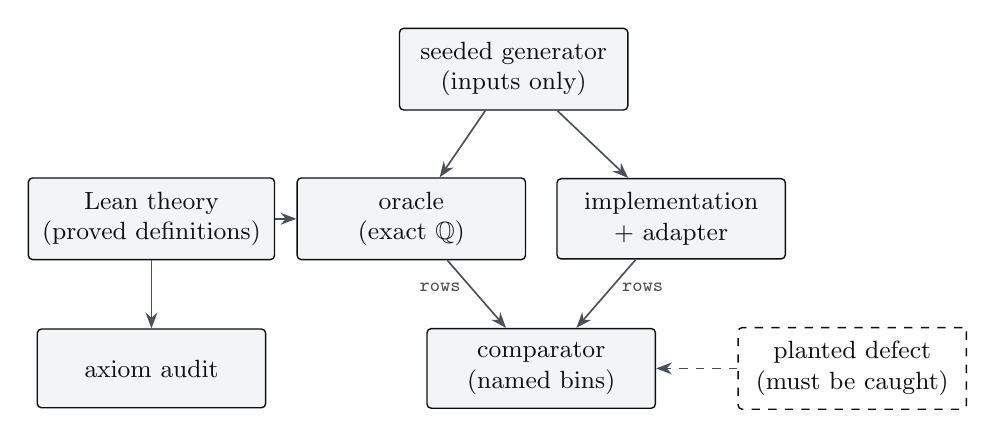
\begin{tikzpicture}[
  box/.style={draw=Ink, line width=0.5pt, fill=Surface, text=Ink, rounded corners=1.5pt,
    align=center, font=\small, inner sep=5pt, minimum height=10mm, minimum width=29mm},
  arr/.style={-{Stealth[length=2mm]}, line width=0.6pt, draw=InkMuted},
  lab/.style={font=\ttfamily\scriptsize, text=InkMuted}]
\node[box] (gen) at (4.6,1.9) {seeded generator\\(inputs only)};
\node[box] (theory) at (0,0) {Lean theory\\(proved definitions)};
\node[box] (oracle) at (3.3,0) {oracle\\(exact $\mathbb{Q}$)};
\node[box] (impl) at (6.6,0) {implementation\\+ adapter};
\node[box] (cmp) at (4.95,-1.9) {comparator\\(named bins)};
\node[box] (audit) at (0,-1.9) {axiom audit};
\node[box, dashed, fill=Background] (planted) at (8.9,-1.9) {planted defect\\(must be caught)};
\draw[arr] (gen) -- (oracle);
\draw[arr] (gen) -- (impl);
\draw[arr] (theory) -- (oracle);
\draw[arr] (theory) -- (audit);
\draw[arr] (oracle) -- node[left, lab, pos=0.4] {rows} (cmp);
\draw[arr] (impl) -- node[right, lab, pos=0.4] {rows} (cmp);
\draw[arr, dashed] (planted) -- (cmp);
\end{tikzpicture}
\caption{The measurement procedure. The generator never computes expected results;
those come only from the oracle.}
\label{fig:harness}
\end{figure}

The procedure follows \texttt{ledger-semantics} (\cref{fig:harness}). A seeded
generator writes case files containing inputs only. It favors the inputs where
implementations are known to have conventions: tied logits, words that are
themselves tokens, and merge tables with several splits of one string. A small
adapter per implementation runs the same cases and prints the oracle's row format.
The comparator places every case in exactly one named bin (agree, diverge, skipped
by either side, or missing), so nothing is dropped silently. Token rows are compared
as strings. Sampler rows require that a zero be matched by a zero and that nonzero
probabilities agree within $10^{-6}$, since llama.cpp stores logits in
\texttt{float32}. Each comparator is observed to fail: a planted defect, an adapter
that glues two tokens or one that inverts temperature, must be detected or the run
fails.

\paragraph{Tie divergences.} An implementation that keeps exactly $k$ tokens breaks
ties in its own order, which need not be the oracle's order by index. Every filter
treats tied tokens alike except for that choice, and tied tokens stay tied through
temperature and renormalization. Such an implementation must therefore agree with
the positional semantics up to a permutation of tied tokens. The harness checks
exactly this: the multiset of (logit, probability) pairs over the kept tokens must
equal that of the oracle's \texttt{q} rows. A divergence that fails this check is
reported as unexplained.

\begin{table}[t]
\centering\small
\caption{Measurements (\texttt{harness/run.sh 600}: four seeds of 600 cases each per
corpus). Lean 4.34.1, Mathlib v4.34.1, \texttt{tokenizers} 0.23.3, \texttt{tiktoken}
0.14.0, llama.cpp commit \texttt{a9d27ac} (2026-10-11).}
\label{tab:results}
\begin{tabularx}{\linewidth}{@{}>{\raggedright\arraybackslash}p{4.6cm}>{\raggedright\arraybackslash}X>{\raggedright\arraybackslash}X@{}}
\toprule
\qpth{Implementation} & \qpth{Compared against} & \qpth{Result}\\
\midrule
HF \texttt{tokenizers}, BPE, defaults & rule-rank BPE (\lean{bpe}) & 13{,}779 / 13{,}779 words identical\\
HF \texttt{tokenizers}, \lean{ignore_merges} & lookup, then rule-rank BPE & 13{,}779 / 13{,}779 identical\\
\texttt{tiktoken} & lookup, then concatenation-rank BPE & 13{,}779 / 13{,}779 identical\\
llama.cpp \lean{top_k}, \lean{top_p}, \lean{min_p}, \texttt{temp}, no ties & tie-keeping filters & 1{,}216 / 1{,}216 chains, $|\Delta p|\le5.1\times10^{-8}$\\
llama.cpp, with ties & tie-keeping, else positional & 939 + 245 / 1{,}184 chains; 0 unexplained\\
Planted defects (tokenizer, sampler) & --- & both detected\\
\bottomrule
\end{tabularx}
\end{table}

\Cref{tab:results} summarizes the results. Two findings came out of the
comparisons. First, \texttt{tiktoken} initially disagreed with the oracle's
concatenation-rank BPE on words that are themselves vocabulary tokens. The
disagreement was a convention, whole-word lookup. Following the
\texttt{ledger-semantics} rule that a divergence is either a defect in the
implementation or a convention the semantics has not yet recorded, we recorded it
as \lean{lookupFirst}, with its own theorems, after which agreement is exact.
Second, on the same random merge tables the two tokenizer libraries disagree with
each other on 439 of 13{,}779 words (3.2\%), and on 279 when Hugging Face uses
\lean{ignore_merges}. The oracle reproduces each library exactly, so every one of
these disagreements is predicted. \Cref{thm:bpeconv} states the condition under which
they cannot occur.

For sampling, llama.cpp agrees with the tie-keeping semantics on every tie-free
chain. On chains with ties, 245 of 1{,}184 diverge, and every one agrees with the
positional semantics up to a permutation of tied tokens. Some of these divergences
cascade: a tie cut by top-$k$ changes the renormalized masses that a later top-$p$
sees. A check that compared kept sets only after the fact would misclassify such
cases. Replaying the convention exactly classifies all of them.

% ===========================================================================
\section{Related work}

\paragraph{Formal methods for machine learning.} Most verification work on neural
networks proves properties of trained models, for example with SMT-based
methods~\cite{katz2017reluplex}. We verify the model-independent algorithms around
the model instead, and connect them to implementations through an oracle. The
denotational method follows Elliott~\cite{elliott2009denotational}. The use of a
proved semantics as a test oracle, the procedure of planted defects, and the
discipline of named skip bins follow \texttt{ledger-semantics}~\cite{ledgersemantics}.
Our category of finite stochastic maps is a special case of Fritz's Markov
categories~\cite{fritz2020markov}.

\paragraph{Tokenization.} Zouhar et al.\ give a formal analysis of BPE as an
optimization problem~\cite{zouhar2023bpe}. Gastaldi et al.\ treat tokenizers as
stochastic maps and study consistency of estimators~\cite{gastaldi2024foundations}.
Vieira et al.\ show how to turn token-level models into character-level
ones~\cite{vieira2024tokens}, which requires exactly the enumeration of
tokenizations we verify. Our no-compression theorem and the agreement criterion
between BPE conventions complement this work at the level of exact identities.

\paragraph{Decoding.} Top-$k$~\cite{fan2018hierarchical}, nucleus~\cite{holtzman2020curious}
and min-$p$~\cite{nguyen2025minp} sampling are usually specified by an algorithm over
sorted arrays, which leaves ties unspecified. \Cref{thm:topk} shows that this gap
cannot be closed by any symmetric rule. Speculative
sampling~\cite{leviathan2023speculative,chen2023speculative} is known to be lossless,
and its acceptance rate is the maximal-coupling bound~\cite{lindvall1992coupling}. Du et
al.\ characterize tightness measure-theoretically~\cite{du2023tight}. We give a
finite-depth statement and an explicit non-tight model.

\paragraph{Attention and inference systems.} Online softmax~\cite{milakov2018online}
underlies FlashAttention~\cite{dao2022flashattention} and its successors, and
KV caching is standard in serving systems~\cite{pope2023scaling,kwon2023vllm}. Our
contribution is the algebraic packaging, a commutative monoid with a free-monoid
homomorphism, and machine-checked proofs over arbitrary exponential characters.
Permutation equivariance of attention without positional encodings is
known~\cite{yun2020universal}.

\paragraph{Masked diffusion.} The time-independence of the optimal denoiser was
observed by Ou et al.~\cite{ou2025absorbing}, in the setting of
D3PM~\cite{austin2021d3pm}, MDLM~\cite{sahoo2024mdlm} and related
models~\cite{shi2024masked,nie2025llada}. We machine-check it, together with the
any-order chain rule and the inexactness of parallel unmasking.

% ===========================================================================
\section{Limitations}

Analysis on the reals enters only through exponential characters, and there is no
measure theory, so sampling and tightness are stated through finite quantities. The
oracle's temperature is restricted to $1/n$, which keeps softmax rational. The
theorems hold for every temperature, but the oracle cannot evaluate an irrational
softmax. Speculative decoding is proved for one drafted token. The sequence version
follows by induction and is not yet formalized. Nothing is proved about
floating-point arithmetic: implementations are compared with exact values within a
stated tolerance. A decision that lies exactly on a floating-point boundary could in
principle diverge, and none occurred in our runs. The diffusion theory covers
absorbing diffusion, not Gaussian diffusion. The chat protocol models tool calling in
its common request-and-result form, not any vendor's specification. The measurements
cover tokenizers and samplers; attention kernels, speculative decoders, chat
renderers and diffusion samplers are evaluated by the oracle but not yet compared
against implementations.

% ===========================================================================
\section{Conclusion}

The inference side of LLMs is small enough to be given a precise meaning and large
enough that its implementations disagree. A machine-checked semantics separates
what is meaning from what is convention. It proves which reorderings, cachings and
tilings are harmless, and it shows that some properties folklore expects, such as
symmetric exact top-$k$, compositional compressing tokenizers and unambiguous plain-text
templates, cannot exist. Connected to an exact oracle, the same definitions become
a test instrument. Every divergence it surfaces is either a defect in an
implementation or a convention that belongs in the semantics.

\paragraph{Availability.} The Lean development, oracle, harness, and recorded
measurement log accompany this paper.

\paragraph{Acknowledgments.} The structure of this work follows
\texttt{ledger-semantics} by John Wiegley. The formalization and harness were
developed with the assistance of an AI system (Claude, Anthropic).

% ===========================================================================
\begin{thebibliography}{99}\small

\bibitem{austin2021d3pm}
J.~Austin, D.~D. Johnson, J.~Ho, D.~Tarlow, and R.~van~den Berg.
\newblock Structured denoising diffusion models in discrete state-spaces.
\newblock In \emph{NeurIPS}, 2021.

\bibitem{chen2023speculative}
C.~Chen, S.~Borgeaud, G.~Irving, J.-B. Lespiau, L.~Sifre, and J.~Jumper.
\newblock Accelerating large language model decoding with speculative sampling.
\newblock arXiv:2302.01318, 2023.

\bibitem{dao2022flashattention}
T.~Dao, D.~Y. Fu, S.~Ermon, A.~Rudra, and C.~R{\'e}.
\newblock {FlashAttention}: Fast and memory-efficient exact attention with {IO}-awareness.
\newblock In \emph{NeurIPS}, 2022.

\bibitem{demoura2021lean4}
L.~de~Moura and S.~Ullrich.
\newblock The {Lean} 4 theorem prover and programming language.
\newblock In \emph{CADE-28}, 2021.

\bibitem{du2023tight}
L.~Du, L.~Torroba~Hennigen, T.~Pimentel, C.~Meister, J.~Eisner, and R.~Cotterell.
\newblock A measure-theoretic characterization of tight language models.
\newblock In \emph{ACL}, 2023.

\bibitem{elliott2009denotational}
C.~Elliott.
\newblock Denotational design with type class morphisms.
\newblock Technical Report 2009-01, LambdaPix, 2009.

\bibitem{fan2018hierarchical}
A.~Fan, M.~Lewis, and Y.~Dauphin.
\newblock Hierarchical neural story generation.
\newblock In \emph{ACL}, 2018.

\bibitem{fritz2020markov}
T.~Fritz.
\newblock A synthetic approach to {Markov} kernels, conditional independence and theorems on sufficient statistics.
\newblock \emph{Advances in Mathematics}, 370, 2020.

\bibitem{gastaldi2024foundations}
J.~L. Gastaldi, J.~Terilla, L.~Malagutti, B.~DuSell, T.~Vieira, and R.~Cotterell.
\newblock The foundations of tokenization: Statistical and computational concerns.
\newblock arXiv:2407.11606, 2024.

\bibitem{greshake2023injection}
K.~Greshake, S.~Abdelnabi, S.~Mishra, C.~Endres, T.~Holz, and M.~Fritz.
\newblock Not what you've signed up for: Compromising real-world {LLM}-integrated applications with indirect prompt injection.
\newblock In \emph{AISec}, 2023.

\bibitem{holtzman2020curious}
A.~Holtzman, J.~Buys, L.~Du, M.~Forbes, and Y.~Choi.
\newblock The curious case of neural text degeneration.
\newblock In \emph{ICLR}, 2020.

\bibitem{katz2017reluplex}
G.~Katz, C.~Barrett, D.~L. Dill, K.~Julian, and M.~J. Kochenderfer.
\newblock Reluplex: An efficient {SMT} solver for verifying deep neural networks.
\newblock In \emph{CAV}, 2017.

\bibitem{kwon2023vllm}
W.~Kwon, Z.~Li, S.~Zhuang, Y.~Sheng, L.~Zheng, C.~H. Yu, J.~E. Gonzalez, H.~Zhang, and I.~Stoica.
\newblock Efficient memory management for large language model serving with {PagedAttention}.
\newblock In \emph{SOSP}, 2023.

\bibitem{ledgersemantics}
J.~Wiegley.
\newblock ledger-semantics: Mathematical semantics of {Ledger}, the double-entry accounting tool.
\newblock \url{https://github.com/ledger/ledger-semantics}, 2026.

\bibitem{leviathan2023speculative}
Y.~Leviathan, M.~Kalman, and Y.~Matias.
\newblock Fast inference from transformers via speculative decoding.
\newblock In \emph{ICML}, 2023.

\bibitem{lindvall1992coupling}
T.~Lindvall.
\newblock \emph{Lectures on the Coupling Method}.
\newblock Wiley, 1992.

\bibitem{liu2023ring}
H.~Liu, M.~Zaharia, and P.~Abbeel.
\newblock Ring attention with blockwise transformers for near-infinite context.
\newblock arXiv:2310.01889, 2023.

\bibitem{mathlib2020}
The mathlib Community.
\newblock The {Lean} mathematical library.
\newblock In \emph{CPP}, 2020.

\bibitem{milakov2018online}
M.~Milakov and N.~Gimelshein.
\newblock Online normalizer calculation for softmax.
\newblock arXiv:1805.02867, 2018.

\bibitem{nguyen2025minp}
M.~N. Nguyen, A.~Baker, C.~Neo, A.~Roush, A.~Kirsch, and R.~Shwartz-Ziv.
\newblock Turning up the heat: Min-p sampling for creative and coherent {LLM} outputs.
\newblock In \emph{ICLR}, 2025.

\bibitem{nie2025llada}
S.~Nie, F.~Zhu, Z.~You, X.~Zhang, J.~Ou, J.~Hu, J.~Zhou, Y.~Lin, J.-R. Wen, and C.~Li.
\newblock Large language diffusion models.
\newblock arXiv:2502.09992, 2025.

\bibitem{ou2025absorbing}
J.~Ou, S.~Nie, K.~Xue, F.~Zhu, J.~Sun, Z.~Li, and C.~Li.
\newblock Your absorbing discrete diffusion secretly models the conditional distributions of clean data.
\newblock In \emph{ICLR}, 2025.

\bibitem{pope2023scaling}
R.~Pope, S.~Douglas, A.~Chowdhery, J.~Devlin, J.~Bradbury, J.~Heek, K.~Xiao, S.~Agrawal, and J.~Dean.
\newblock Efficiently scaling transformer inference.
\newblock In \emph{MLSys}, 2023.

\bibitem{rabe2021selfattention}
M.~N. Rabe and C.~Staats.
\newblock Self-attention does not need {$O(n^2)$} memory.
\newblock arXiv:2112.05682, 2021.

\bibitem{radford2019gpt2}
A.~Radford, J.~Wu, R.~Child, D.~Luan, D.~Amodei, and I.~Sutskever.
\newblock Language models are unsupervised multitask learners.
\newblock OpenAI technical report, 2019.

\bibitem{sahoo2024mdlm}
S.~S. Sahoo, M.~Arriola, Y.~Schiff, A.~Gokaslan, E.~Marroquin, J.~T. Chiu, A.~Rush, and V.~Kuleshov.
\newblock Simple and effective masked diffusion language models.
\newblock In \emph{NeurIPS}, 2024.

\bibitem{sennrich2016bpe}
R.~Sennrich, B.~Haddow, and A.~Birch.
\newblock Neural machine translation of rare words with subword units.
\newblock In \emph{ACL}, 2016.

\bibitem{shi2024masked}
J.~Shi, K.~Han, Z.~Wang, A.~Doucet, and M.~K. Titsias.
\newblock Simplified and generalized masked diffusion for discrete data.
\newblock In \emph{NeurIPS}, 2024.

\bibitem{vieira2024tokens}
T.~Vieira, B.~LeBrun, M.~Giulianelli, J.~L. Gastaldi, B.~DuSell, J.~Terilla, T.~J. O'Donnell, and R.~Cotterell.
\newblock From language models over tokens to language models over characters.
\newblock arXiv:2412.03719, 2024.

\bibitem{wolf2020transformers}
T.~Wolf et~al.
\newblock Transformers: State-of-the-art natural language processing.
\newblock In \emph{EMNLP: System Demonstrations}, 2020.

\bibitem{xiao2024sinks}
G.~Xiao, Y.~Tian, B.~Chen, S.~Han, and M.~Lewis.
\newblock Efficient streaming language models with attention sinks.
\newblock In \emph{ICLR}, 2024.

\bibitem{yun2020universal}
C.~Yun, S.~Bhojanapalli, A.~S. Rawat, S.~J. Reddi, and S.~Kumar.
\newblock Are transformers universal approximators of sequence-to-sequence functions?
\newblock In \emph{ICLR}, 2020.

\bibitem{zouhar2023bpe}
V.~Zouhar, C.~Meister, J.~L. Gastaldi, L.~Du, T.~Vieira, M.~Sachan, and R.~Cotterell.
\newblock A formal perspective on byte-pair encoding.
\newblock In \emph{Findings of ACL}, 2023.

\end{thebibliography}

\end{document}
"

\usepackage[a4paper,textwidth=15.4cm,textheight=23.6cm,top=3.0cm,headsep=0.9cm,footskip=1.2cm]{geometry}
\usepackage{amsmath,amssymb,amsthm,mathtools}
\usepackage{fontspec}
\usepackage{booktabs,tabularx,array}
\usepackage[protrusion=true,expansion=false]{microtype}
\usepackage[table]{xcolor}
\usepackage{graphicx}
\usepackage{fvextra}
\usepackage{enumitem}
\usepackage{caption}
\usepackage{titlesec}
\usepackage{fancyhdr}
\usepackage[most]{tcolorbox}
\usepackage{tikz}
\usetikzlibrary{arrows.meta}
\usepackage{hyperref}
\usepackage[nameinlink,capitalise]{cleveref}

% ---------------------------------------------------------------------------
%  Colour tokens
% ---------------------------------------------------------------------------
% Neutral foundation. Ink and Background invert between the two editions.
\ifqptdark
  \definecolor{Background}{HTML}{0B0C0E}
  \definecolor{Surface}{HTML}{16181B}
  \definecolor{Border}{HTML}{2B2E33}
  \definecolor{Ink}{HTML}{EDEEF0}
  \definecolor{InkMuted}{HTML}{A9AEB6}
  \definecolor{InkFaint}{HTML}{5A5F67}   % decoration only, never meaningful text
\else
  \definecolor{Background}{HTML}{FFFFFF}
  \definecolor{Surface}{HTML}{F3F4F5}
  \definecolor{Border}{HTML}{DADDE1}
  \definecolor{Ink}{HTML}{0E0F11}
  \definecolor{InkMuted}{HTML}{4B4F57}
  \definecolor{InkFaint}{HTML}{A3A7AE}   % decoration only, never meaningful text
\fi
% Paradigm colours: fixed in both editions, semantic only.
\definecolor{Quantum}{HTML}{5BAD1E}
\definecolor{Photonic}{HTML}{F0AB00}
\definecolor{Thermodynamic}{HTML}{E8690A}
\definecolor{Ternary}{HTML}{8A8A8A}
\definecolor{Bio}{HTML}{1AAB7C}

\ifqptdark\pagecolor{Background}\fi

% ---------------------------------------------------------------------------
%  Typography
% ---------------------------------------------------------------------------
\setmainfont{Inter}[
  Path=fonts/, Extension=.otf, Scale=0.94,
  UprightFont=*-Regular, ItalicFont=*-Italic,
  BoldFont=*-SemiBold, BoldItalicFont=*-SemiBoldItalic]
\setmonofont{IBMPlexMono}[
  Path=fonts/, Extension=.ttf, Scale=MatchLowercase,
  UprightFont=*-Regular, ItalicFont=*-Italic, BoldFont=*-SemiBold]
\newfontfamily\qptdisplay{SpaceGrotesk}[
  Path=fonts/, Extension=.otf, UprightFont=*-Medium, BoldFont=*-Bold]
\newfontfamily\qptdisplaylight{SpaceGrotesk}[
  Path=fonts/, Extension=.otf, UprightFont=*-Regular]
\newfontfamily\qptlabelfont{IBMPlexMono}[
  Path=fonts/, Extension=.ttf, Scale=MatchLowercase, UprightFont=*-Medium,
  LetterSpace=6]
\setsansfont{Inter}[
  Path=fonts/, Extension=.otf, Scale=0.94,
  UprightFont=*-Regular, ItalicFont=*-Italic,
  BoldFont=*-SemiBold, BoldItalicFont=*-SemiBoldItalic]
\linespread{1.16}
\setlength{\emergencystretch}{2.5em}
\AtBeginDocument{\raggedright\setlength{\parindent}{0pt}}
\setlength{\parindent}{0pt}
\setlength{\parskip}{0.55em}

% A label: IBM Plex Mono, upper case, tracked.
\newcommand{\qptlabel}[1]{{\qptlabelfont\footnotesize\MakeUppercase{#1}}}
% Technical names (Lean declarations, files) in IBM Plex Mono.
\newcommand{\lean}[1]{\texttt{\detokenize{#1}}}
\newcommand{\leanref}[1]{\par\smallskip\noindent
  {\ttfamily\footnotesize\upshape\raggedright\color{InkMuted}LEAN\enspace #1\par}}

% Ink is the normal colour everywhere, including floats, heads and footnotes.
\makeatletter
\AtBeginDocument{\color{Ink}\global\let\default@color\current@color}
\makeatother

% ---------------------------------------------------------------------------
%  Mathematical notation
% ---------------------------------------------------------------------------
\newcommand{\K}{\Bbbk}
\newcommand{\Dist}{\mathrm{Dist}}
\newcommand{\restr}[2]{#1|_{#2}}
\newcommand{\topk}{\mathrm{TopK}}
\newcommand{\topp}{\mathrm{TopP}}
\newcommand{\minp}{\mathrm{MinP}}
\newcommand{\sharpen}{\mathrm{sharpen}}
\newcommand{\abv}{\mathrm{above}}
\newcommand{\tv}{\mathrm{tv}}
\newcommand{\dec}{\mathrm{dec}}
\newcommand{\enc}{\mathrm{enc}}
\newcommand{\softmax}{\mathrm{softmax}}
\newcommand{\attend}{\mathrm{attend}}
\newcommand{\Iv}[1]{[\![#1]\!]}
\newcommand{\Mask}{\bot}

% ---------------------------------------------------------------------------
%  Headings: section numbers as labels, titles in Space Grotesk
% ---------------------------------------------------------------------------
\makeatletter
\newcommand{\qptsecnum}[1]{{\qptlabelfont\small\color{InkMuted}\two@digits{#1}}}
\makeatother
\titleformat{\section}
  {\qptdisplay\fontsize{14.5}{18}\selectfont\color{Ink}}
  {\qptsecnum{\value{section}}}{0.9em}{}
\titleformat{name=\section,numberless}
  {\qptdisplay\fontsize{14.5}{18}\selectfont\color{Ink}}{}{0pt}{}
\titlespacing*{\section}{0pt}{1.9em}{0.7em}
\titleformat{\paragraph}[runin]
  {\qptdisplay\normalsize\color{Ink}}{}{0pt}{}
\titlespacing*{\paragraph}{0pt}{0.9em}{0.6em}

% ---------------------------------------------------------------------------
%  Statements
% ---------------------------------------------------------------------------
\newtheoremstyle{qpt}
  {0.9em}{0.9em}
  {\normalfont}{}
  {\qptlabelfont\footnotesize}{}
  {\newline}
  {\MakeUppercase{\thmname{#1}\thmnumber{~#2}}%
   \thmnote{\enspace{\qptdisplay\normalsize\color{Ink}#3}}}
\theoremstyle{qpt}
\newtheorem{theorem}{Theorem}
\newtheorem{proposition}[theorem]{Proposition}
\newtheorem{corollary}[theorem]{Corollary}
\newtheorem{lemma}[theorem]{Lemma}
\newtheorem{definition}[theorem]{Definition}
\newtheorem{remark}[theorem]{Remark}

% Proofs: a tracked label and a neutral end mark.
\makeatletter
\renewcommand{\qedsymbol}{{\color{InkMuted}\rule{0.5em}{0.5em}}}
\renewenvironment{proof}[1][Proof]{\par\pushQED{\qed}\normalfont\topsep0.5em\relax
  \trivlist\item[\hskip\labelsep\qptlabel{#1}\hspace{0.6em}]\ignorespaces}
  {\popQED\endtrivlist\@endpefalse}
\makeatother

% ---------------------------------------------------------------------------
%  Code: IBM Plex Mono on a neutral surface, with a hairline on the left
% ---------------------------------------------------------------------------
\tcbset{colupper=Ink, collower=Ink}
\tcbset{qptcode/.style={enhanced, colback=Surface, colframe=Surface,
  boxrule=0pt, arc=0pt, left=9pt, right=8pt, top=5pt, bottom=5pt,
  borderline west={1.2pt}{0pt}{InkFaint}, before skip=0.7em, after skip=0.7em}}
\newenvironment{leancode}
  {\VerbatimEnvironment\begin{tcolorbox}[qptcode]%
   \begin{Verbatim}[fontsize=\small,commandchars=\\\{\},
     codes={\catcode`\$=3\catcode`\^=7},formatcom=\color{Ink}]}
  {\end{Verbatim}\end{tcolorbox}}
\newenvironment{casecode}
  {\VerbatimEnvironment\begin{tcolorbox}[qptcode,before skip=0pt,after skip=0pt]%
   \begin{Verbatim}[fontsize=\footnotesize,formatcom=\color{Ink}]}
  {\end{Verbatim}\end{tcolorbox}}

% ---------------------------------------------------------------------------
%  Floats, tables, captions
% ---------------------------------------------------------------------------
\DeclareCaptionLabelFormat{qpt}{\qptlabel{#1~#2}}
\DeclareCaptionLabelSeparator{qptsep}{\quad}
\captionsetup{labelformat=qpt, labelsep=qptsep, font={small,color=Ink},
  justification=raggedright, singlelinecheck=false, skip=6pt}
\newcommand{\qpth}[1]{\qptlabel{#1}}
\arrayrulecolor{Ink}
\setlength{\heavyrulewidth}{0.7pt}
\setlength{\lightrulewidth}{0.35pt}
\renewcommand{\arraystretch}{1.22}

% ---------------------------------------------------------------------------
%  Running heads
% ---------------------------------------------------------------------------
\pagestyle{fancy}
\fancyhf{}
\fancyhead[L]{{\color{Ink}\qptlabel{Machine-checked semantics of LLM inference}}}
\fancyhead[R]{{\color{Ink}\qptlabel{D. Arango Sohm}}}
\fancyfoot[R]{{\ttfamily\small\color{InkMuted}\thepage}}
\renewcommand{\headrule}{{\color{Border}\hrule height 0.4pt}\vspace{-0.4pt}}
\renewcommand{\headrulewidth}{0.4pt}
\fancypagestyle{qptfirst}{\fancyhf{}%
  \fancyfoot[R]{{\ttfamily\small\color{InkMuted}\thepage}}%
  \renewcommand{\headrulewidth}{0pt}\renewcommand{\headrule}{}}

% ---------------------------------------------------------------------------
%  Links and references: neutral, never accent-coloured text
% ---------------------------------------------------------------------------
\hypersetup{colorlinks=true, linkcolor=Ink, citecolor=Ink, urlcolor=Ink,
  pdftitle={A Machine-Checked Semantics of LLM Inference},
  pdfauthor={Daniel Arango Sohm},
  pdfsubject={Formal semantics of large language model inference in Lean 4},
  pdfkeywords={Lean 4, Mathlib, formal verification, LLM inference, sampling,
    tokenization, attention, speculative decoding, diffusion language models}}
\makeatletter
\renewcommand{\@biblabel}[1]{{\ttfamily\color{InkMuted}[#1]}}
\renewcommand{\@cite}[2]{{\ttfamily[#1\if@tempswa, #2\fi]}}
\makeatother
\renewcommand{\refname}{References}

\setlist{itemsep=2pt, topsep=4pt}
\setlist[itemize]{label={\color{InkMuted}\textbullet}}

\begin{document}
\thispagestyle{qptfirst}

% ----------------------------------------------------------------- masthead
\noindent
\begin{minipage}[c]{0.5\linewidth}
  \includegraphics[height=1.9cm]{qpt-logo.png}
\end{minipage}%
\begin{minipage}[c]{0.5\linewidth}\raggedleft
  \qptlabel{Preprint}\\[2pt]
  \qptlabel{October 2026}
\end{minipage}

\vspace{1.6em}
{\color{Border}\rule{\linewidth}{0.4pt}}
\vspace{1.1em}

{\qptdisplay\fontsize{25}{29.5}\selectfont\color{Ink}
A Machine-Checked Semantics\\ of LLM Inference\par}
\vspace{0.55em}
{\qptdisplaylight\fontsize{13}{17}\selectfont\color{InkMuted}
Sampling, Attention, Tokenization, Chat, Decoding,\\ and Diffusion in Lean~4\par}

\vspace{1.5em}
{\large\bfseries Daniel Arango Sohm}\par
\vspace{0.15em}
{\color{InkMuted}Universidad EAFIT, Medellín, Colombia\\
Former member of the QPT team}\par

\vspace{1.4em}
% ----------------------------------------------------------------- abstract
\begin{tcolorbox}[enhanced, colback=Surface, colframe=Surface, colupper=Ink, boxrule=0pt,
  arc=0pt, left=12pt, right=12pt, top=9pt, bottom=10pt]
\qptlabel{Abstract}\par\vspace{0.35em}
{\small
The inference side of a large language model is a stack of small algorithms:
tokenizers, attention kernels, key--value caches, sampling filters, speculative
decoders, chat templates, and diffusion samplers. Each has several independent
implementations, and those implementations are usually tested against one another
rather than against a definition. We give these components a single mathematical
semantics, formalized in Lean~4 against Mathlib. The development comprises about
4{,}600 lines and 270 named theorems, and every declaration depends only on Lean's
three standard axioms. It proves the exact algebra of sampling filters, the
losslessness and optimality of speculative sampling, and the correctness of
key--value caching and of FlashAttention-style online softmax as a commutative
monoid. It proves that byte-pair encoding is lossless under every merge priority,
together with a decidable criterion for when the Hugging Face and \texttt{tiktoken}
conventions agree, a protocol checker for tool calls, and the time-independence of
the masked-diffusion denoiser. It also proves six negative results. No sampling
rule that treats tokens symmetrically can always keep exactly $k$ tokens. No
tokenizer that compresses can respect concatenation. Every chat template that writes
its role markers in the content alphabet is ambiguous. No transformer without
positional information can copy a fixed position. An autoregressive model need not
define a distribution over strings. Parallel unmasking in diffusion is inexact.
From the same definitions we build an executable oracle that evaluates test cases in
exact rational arithmetic, and a harness that measures implementations against it.
On 2{,}400 random merge tables, Hugging Face \texttt{tokenizers} and
\texttt{tiktoken} each agree with the oracle on all 13{,}779 test words, while
disagreeing with each other on 3.2\% of them. On 2{,}400 random sampler chains,
every divergence of llama.cpp from the tie-keeping semantics is accounted for
exactly by the positional semantics that the impossibility theorem forces.
\par}
\end{tcolorbox}

\vspace{0.3em}
\noindent\qptlabel{Keywords}\enspace{\small Lean~4 · Mathlib · formal verification ·
LLM inference · sampling · tokenization · attention · speculative decoding ·
diffusion language models}

\vspace{0.4em}
{\color{Border}\rule{\linewidth}{0.4pt}}

% ===========================================================================
\section{Introduction}

A deployed language model is a function from parameters and a context to a
distribution over tokens. Turning that distribution into text requires more
machinery. A tokenizer maps strings to token sequences. Attention kernels compute
the model's reads over a cached context. A chain of sampling filters reshapes the
next-token distribution. A speculative decoder may verify drafted tokens, a chat
template linearizes a conversation, and a diffusion sampler may unmask several
positions at once. Each of these components exists in many implementations, such as
Hugging Face \texttt{transformers} and \texttt{tokenizers}~\cite{wolf2020transformers},
\texttt{tiktoken}, vLLM~\cite{kwon2023vllm}, and llama.cpp. Their tests mostly
compare one implementation with another, or with remembered behavior.

This paper follows a different discipline, \emph{denotational design}~\cite{elliott2009denotational}.
One first says precisely what a thing means, then requires every operation to
preserve that meaning, and lets the implementation be whatever the equations force
it to be. The approach is that of \texttt{ledger-semantics}~\cite{ledgersemantics},
which formalizes double-entry accounting in Lean and uses the result as a test oracle
for the C++ Ledger program. We apply it to LLM inference. A sampling filter means
conditioning a distribution on a set. A KV-cached decoder means causal attention over
the whole prefix. A FlashAttention kernel means a softmax-weighted average. A chat
template means an injective encoding of a transcript. The theorems state when an
implementation preserves that meaning, and several of them state that no
implementation can.

\paragraph{Contributions.}
\begin{itemize}[leftmargin=*,itemsep=2pt]
\item A Lean~4 formalization against Mathlib~\cite{mathlib2020,demoura2021lean4}
  of sampling, speculative decoding, softmax and attention, tokenization, chat
  transcripts, autoregressive decoding, and masked diffusion
  (\cref{sec:foundations,sec:sampling,sec:spec,sec:attention,sec:tokenization,sec:chat,sec:decoding,sec:diffusion}).
  All definitions are stated over an arbitrary linearly ordered field, so one proof
  covers the real numbers of the literature and the exact rationals of the oracle.
\item Positive results in a common framework. They include the algebra of
  sampling filters, the optimality of speculative sampling, an online-softmax
  commutative monoid, a generic correctness theorem for BPE with a decidable
  agreement criterion between the two conventions in use, a protocol checker for
  tool calls, and the any-order chain rule for masked diffusion.
\item Six negative results that explain design constraints visible across
  implementations (\cref{sec:negative}).
\item An executable oracle that evaluates case files under the proved
  definitions in exact arithmetic, and a measurement of Hugging Face
  \texttt{tokenizers}, \texttt{tiktoken}, and llama.cpp against it (\cref{sec:oracle,sec:measure}).
\end{itemize}

Several of the positive results are known: losslessness of speculative
sampling~\cite{leviathan2023speculative,chen2023speculative}, correctness of online
softmax~\cite{milakov2018online,dao2022flashattention}, time-independence of the
absorbing-diffusion posterior~\cite{ou2025absorbing}, and the role of permutation
equivariance~\cite{yun2020universal}. Our contribution for these is a machine-checked
statement in one framework, connected to an oracle. To our knowledge the
following are not stated elsewhere in the form given here: the impossibility of
symmetric exact top-$k$ and nucleus selection, the no-compression theorem for
homomorphic tokenizers, the ambiguity of every in-band chat template, and the
decidable agreement criterion between merge-rule and concatenation-rank BPE.

% ===========================================================================
\section{Method and trust base}\label{sec:method}

The development is a Lean~4 library (Lean 4.34.1, Mathlib v4.34.1) of eleven
theory modules and two executable modules (\cref{tab:modules}). It is built with
warnings promoted to errors, so an unproved theorem (\lean{sorry}) fails the build.
A separate audit program walks every declaration in the library, 853 in all, and
fails unless each depends only on propositional extensionality, the axiom of choice,
and quotient soundness. The audit has been observed to fail: a planted proof by
\lean{native_decide}, which introduces an auxiliary axiom trusting compiled code, is
rejected. The warnings-as-errors build alone does not catch it. Concrete
counterexamples are therefore proved by \lean{decide}, whose certificate the kernel
checks by evaluation.

\begin{table}[t]
\centering\small
\caption{Modules of the development. Lines and named theorems and lemmas per module.}
\label{tab:modules}
\begin{tabularx}{\linewidth}{@{}l>{\raggedright\arraybackslash}X>{\ttfamily}r>{\ttfamily}r@{}}
\toprule
\qpth{Module} & \qpth{Content} & \qpth{Lines} & \qpth{Thms} \\
\midrule
\lean{Dist} & finite distributions, conditioning, total variation, $\mathsf{FinStoch}$ & 383 & 34\\
\lean{Sampling} & top-$k$, top-$p$, min-$p$, temperature, ties, inverse CDF & 732 & 46\\
\lean{Counterexamples} & kernel-checked failures of sampler laws & 52 & 4\\
\lean{Speculative} & speculative sampling, couplings & 194 & 17\\
\lean{Softmax} & exponential characters, masking, temperature & 220 & 23\\
\lean{Attention} & equivariance, causality, KV cache, online softmax & 573 & 38\\
\lean{Real} & $\exp$ as a character; textbook restatements & 51 & 4\\
\lean{Tokenization} & free-monoid decoding, BPE conventions, enumeration & 860 & 49\\
\lean{Chat} & tool-call protocol, rendering & 440 & 21\\
\lean{Decoding} & mass conservation, tightness, greedy decoding & 245 & 15\\
\lean{Diffusion} & masked diffusion, posterior, chain rule & 379 & 18\\
\lean{Oracle}, \lean{Driver} & case parsing and exact evaluation & 465 & 1\\
\midrule
Total & & 4{,}594 & 270\\
\bottomrule
\end{tabularx}
\end{table}

\paragraph{Numbers.} Every probability lives in an arbitrary field $\K$ with a
compatible linear order (\lean{[Field K] [LinearOrder K] [IsStrictOrderedRing K]}).
The oracle instantiates $\K=\mathbb{Q}$, so its arithmetic is exact. The analytic
statements instantiate $\K=\mathbb{R}$. No measure theory is used. Sampling is made
precise through interval statements (\cref{thm:invcdf}), and tightness through
masses at finite depth (\cref{sec:decoding}).

% ===========================================================================
\section{Foundations}\label{sec:foundations}

\begin{definition}[Finite distribution]
For a finite type $\alpha$, $\Dist_\K(\alpha)$ is the type of functions
$p:\alpha\to\K$ with $p(a)\ge 0$ for all $a$ and $\sum_a p(a)=1$.
\leanref{\lean{Dist}}
\end{definition}

\begin{leancode}
structure Dist ($\K$ : Type u) [Field $\K$] [LinearOrder $\K$] [IsStrictOrderedRing $\K$]
    ($\alpha$ : Type v) [Fintype $\alpha$] where
  prob : $\alpha$ $\to$ $\K$
  nonneg : $\forall$ a, 0 $\le$ prob a
  sum_eq_one : $\sum$ a, prob a = 1
\end{leancode}

The single operation through which masks, filters and grammar constraints act is
conditioning. For $S\subseteq\alpha$ with $p(S)>0$, write
$\restr{p}{S}(a)=\Iv{a\in S}\,p(a)/p(S)$ (\lean{Dist.restrict}).

\begin{lemma}[Conditioning]\label{lem:restrict}
$\restr{(\restr{p}{S})}{T}=\restr{p}{S\cap T}$ whenever the masses involved are
positive. Moreover $\restr{p}{S}=\restr{p}{S'}$ whenever $S$ and $S'$ contain the same
outcomes of positive probability.
\leanref{\lean{restrict_restrict}, \lean{restrict_congr}}
\end{lemma}

The finite distribution monad (point masses and \lean{bind}) satisfies the monad
laws. Finite types and stochastic maps $\alpha\to\Dist_\K(\beta)$ form a category
$\mathsf{FinStoch}_\K$, given as an instance of Mathlib's \lean{Category} whose
composition is Kleisli composition (\lean{FinStoch.category}). Total variation is
$\tv(p,q)=\sum_a\max(0,p(a)-q(a))$. We prove
$\tv(p,q)=\tfrac12\sum_a|p(a)-q(a)|$, $\sum_a\min(p(a),q(a))=1-\tv(p,q)$, and
$\tv(p,q)=0\iff p=q$.

% ===========================================================================
\section{Sampling}\label{sec:sampling}

Let $V$ be a finite vocabulary and $p:V\to\K$. Write
$\abv_p(v)=\{u: p(v)<p(u)\}$ for the tokens strictly preferred to $v$. The three
standard filters keep the sets
\begin{gather*}
\topk_k(p)=\{v: |\abv_p(v)|<k\},\qquad
\minp_m(p)=\{v:\forall u,\; m\,p(u)\le p(v)\},\\
\topp_P(p)=\Bigl\{v: \textstyle\sum_{u\in\abv_p(v)}p(u)<P\Bigr\},
\end{gather*}
and the filtered distribution is the conditioning $\restr{p}{S}$ on the kept set
$S$. For distinct probabilities, $\topp_P$ is the usual rule ``sort in descending
order and keep the shortest prefix whose mass reaches $P$''. With ties, all three
keep every tied token. Temperature $1/n$ is
$\sharpen_n(p)(v)=p(v)^n/\sum_u p(u)^n$, which stays inside $\mathbb{Q}$. In
\cref{sec:attention} we show that it equals $\softmax(n\cdot z)$ when
$p=\softmax(z)$. Every kept set contains a most probable token, provided $k\ge1$,
$P>0$ and $m\le1$, so no filter can produce an empty distribution.

\begin{theorem}[Sampler algebra]\label{thm:algebra}
For $k,k'\ge1$, $m,m'\le1$ and $n\ge1$, and writing filters in the order they are
applied,
\begin{enumerate}[label=(\roman*),itemsep=1pt]
\item top-$k$ then top-$k'$ equals top-$\min(k,k')$;
\item min-$m$ then min-$m'$ equals min-$\max(m,m')$; in particular both filters are idempotent;
\item top-$k$ and min-$m$ commute;
\item top-$k$ and temperature $1/n$ commute.
\end{enumerate}
\leanref{\lean{topK_topK}, \lean{minP_minP}, \lean{topK_minP_comm}, \lean{topK_sharpen_comm}}
\end{theorem}

\begin{proof}[Proof sketch]
All three kept sets are \emph{upward closed}: if $v$ is kept and $p(v)<p(u)$, then
$u$ is kept. Conditioning on an upward-closed set $S$ leaves $\abv(v)$ unchanged for
$v\in S$ (\lean{above_restrict}), and min-$p$ is insensitive to conditioning on a set
that contains a maximizer (\lean{minP_restrict_iff}). Each identity then reduces,
through \cref{lem:restrict}, to an equality of kept sets. For (iv), $x\mapsto x^n$
is strictly increasing on $[0,\infty)$, and top-$k$ depends only on the order of the
scores (\lean{topKSet_congr}).
\end{proof}

The laws one might expect beyond \cref{thm:algebra} are false. With
$p_0=(\tfrac12,\tfrac3{10},\tfrac15)$, the kernel evaluates the following
(\lean{Counterexamples}).

\begin{proposition}[Failed laws]\label{prop:counter}
\leavevmode\vspace{-0.5\baselineskip}
\begin{enumerate}[label=(\roman*),itemsep=1pt]
\item Top-$p$ is not idempotent: one pass of $\topp_{3/5}$ gives token~1 the probability $\tfrac38$, and a second pass gives it~$0$.
\item Top-$p$ does not commute with top-$k$: top-$p$ then top-2 leaves token~1 at $\tfrac38$, while top-2 then top-$p$ removes it.
\item Top-$p$ does not commute with temperature $\tfrac12$: token~1 ends at $\tfrac9{34}$ in one order and at $0$ in the other.
\item Min-$p$ ($m=\tfrac12$) does not commute with temperature $\tfrac12$, with the same numbers.
\end{enumerate}
\end{proposition}

A sampler chain may therefore reorder top-$k$, min-$p$ and temperature only as
\cref{thm:algebra} allows, and may not move top-$p$ at all.

\paragraph{Ties.} Implementations differ on ties, and the difference is forced.
Call a selection rule $\mathrm{sel}:(V\to\K)\to\mathcal{P}(V)$ \emph{equivariant} if
$\mathrm{sel}(p\circ\sigma^{-1})=\sigma[\mathrm{sel}(p)]$ for every permutation
$\sigma$ of $V$, that is, if relabeling the tokens relabels the output.

\begin{theorem}[No symmetric exact top-$k$]\label{thm:topk}
Let $0<k<|V|$. No equivariant selection rule satisfies $|\mathrm{sel}(p)|=k$ for
every distribution $p$.
\leanref{\lean{no_equivariant_exact_topK}}
\end{theorem}
\begin{proof}
On the uniform distribution $u$ we have $u\circ\sigma^{-1}=u$ for every $\sigma$, so
$\mathrm{sel}(u)$ is invariant under all permutations. If it contains some $v$, then
for any $w$ the transposition $(v\,w)$ maps $v$ to $w$, so it contains $w$ too.
Hence $\mathrm{sel}(u)$ is either empty or all of $V$, and neither has $k$ elements.
\end{proof}

\begin{leancode}
theorem no_equivariant_exact_topK [DecidableEq V] \char123{}k : $\mathbb{N}$\char125{}
    (hk0 : 0 < k) (hkn : k < Fintype.card V)
    (sel : (V $\to$ $\K$) $\to$ Finset V) (hsel : Equivariant sel) :
    $\neg$ $\forall$ d : Dist $\K$ V, (sel d.prob).card = k
\end{leancode}

\begin{theorem}[No symmetric smallest nucleus]
Let $V$ be nonempty and $0<P\le1-1/|V|$. No equivariant rule returns, for every
distribution, a set of minimum cardinality among those of mass at least~$P$.
\leanref{\lean{no_equivariant_exact_nucleus}}
\end{theorem}

The tie-keeping filters are equivariant (\lean{topKSet_equivariant}). The other
option is to break ties by position. Define $u\prec_p v$ if $p(u)>p(v)$, or if
$p(u)=p(v)$ and $u<v$, and let the positional filters count predecessors under
$\prec_p$ instead of $\abv_p$ (\lean{Dist.topKPos}, \lean{Dist.topPPos}).

\begin{theorem}[Positional tie-breaking]
Positional top-$k$ keeps exactly $\min(k,|V|)$ tokens. If $p$ is injective, the
positional and tie-keeping filters coincide. For $0<k<|V|$, positional top-$k$ is
not equivariant.
\leanref{\lean{card_topKPosSet}, \lean{topKPosSet_eq_of_injective}, \lean{topPPosSet_eq_of_injective}, \lean{topKPosSet_not_equivariant}}
\end{theorem}

An implementation must therefore choose between keeping exactly $k$ tokens and
treating tokens symmetrically. Hugging Face \texttt{transformers} (read from the
source of version 5.19.0) keeps ties in top-$k$, since it removes only scores
strictly below the $k$-th largest, but breaks them by sort position in top-$p$.
llama.cpp breaks ties by position in both, as measured in \cref{sec:measure}.

\begin{theorem}[Inverse-CDF sampling]\label{thm:invcdf}
Let $F(i)=\sum_{j<i}p(j)$ on $V=\{0,\dots,n-1\}$ and let $\iota(u)$ be the least $i$
with $u<F(i+1)$. For $0\le u<1$, $\iota(u)=i\iff F(i)\le u<F(i+1)$, and
$F(i+1)-F(i)=p(i)$. A uniform $u$ therefore selects $i$ with probability $p(i)$.
\leanref{\lean{invCdf_eq_iff}, \lean{cdf_interval_length}}
\end{theorem}

% ===========================================================================
\section{Speculative decoding}\label{sec:spec}

A draft model proposes $x\sim q$. The target, with distribution $p$, accepts with
probability $a(x)=\min(1,p(x)/q(x))$, and on rejection a token is drawn from the
residual $r=(p-q)^+/\tv(p,q)$~\cite{leviathan2023speculative,chen2023speculative}.
We define the joint law of (draft, emitted token) exactly as the algorithm runs,
\[
\pi(x,y)=q(x)\bigl(a(x)\,\Iv{y=x}+(1-a(x))\,r(y)\bigr).
\]

\begin{theorem}[Speculative sampling]
\leavevmode\vspace{-0.5\baselineskip}
\begin{enumerate}[label=(\roman*),itemsep=1pt]
\item The draft has law $q$: $\sum_y\pi(x,y)=q(x)$.
\item \emph{Losslessness}: the emitted token has law $p$: $\sum_x\pi(x,y)=p(y)$.
\item The acceptance probability is $\sum_x q(x)a(x)=1-\tv(p,q)$, and the emitted token equals the draft with the same probability.
\item \emph{Optimality}: every coupling $\gamma$ of $q$ and $p$ has $\sum_x\gamma(x,x)\le1-\tv(p,q)$.
\end{enumerate}
\leanref{\lean{specJoint_fst}, \lean{specJoint_snd}, \lean{accept_rate}, \lean{specJoint_diag}, \lean{coupling_le}, \lean{spec_optimal}}
\end{theorem}
\begin{proof}[Proof sketch]
Since $q(x)a(x)=\min(p(x),q(x))$, the total rejection probability is $\tv(p,q)$,
and a rejected draft is never re-emitted, because $r(x)=0$ whenever $q(x)>p(x)$. For (iv),
$\gamma(x,x)\le\min(q(x),p(x))$ by the marginal constraints. This is the classical
coupling inequality~\cite{lindvall1992coupling}.
\end{proof}

Because any lossless rule for verifying one drafted token is a coupling, (iv) shows
that speculative sampling has the highest acceptance rate any such rule can achieve.

% ===========================================================================
\section{Softmax and attention}\label{sec:attention}

\begin{definition}[Exponential character]
An \emph{exponential character} from an ordered additive group $G$ of scores into
$\K$ is a strictly increasing map $E:G\to\K$ with $E(a)>0$ and $E(a+b)=E(a)E(b)$.
For $z:\iota\to G$, $\softmax_E(z)_i=E(z_i)/\sum_jE(z_j)$.
\leanref{\lean{ExpChar}}
\end{definition}

$\exp:\mathbb{R}\to\mathbb{R}$ is a character (\lean{ExpChar.real}). So is
$z\mapsto2^z:\mathbb{Z}\to\mathbb{Q}$ (\lean{ExpChar.base2}), which the oracle uses
to evaluate softmax with no rounding. Every result in this section holds for every
character, and so for both.

\begin{theorem}[Softmax]\label{thm:softmax}
\leavevmode\vspace{-0.5\baselineskip}
\begin{enumerate}[label=(\roman*),itemsep=1pt]
\item $\softmax_E(z+c)=\softmax_E(z)$; this licenses subtracting the maximum logit.
\item $\softmax_E(z)_i<\softmax_E(z)_j\iff z_i<z_j$.
\item \emph{Masking is conditioning}: setting logits outside $S$ to $-\infty$ and taking softmax gives $\restr{\softmax_E(z)}{S}$.
\item For $G$ a field and $T>0$, $\topk_k(\softmax_E(z/T))=\topk_k(z)$.
\item $\softmax_E(n\cdot z)=\sharpen_n(\softmax_E(z))$.
\end{enumerate}
\leanref{\lean{softmax_add_const}, \lean{softmax_lt_iff}, \lean{softmaxOn_eq_restrict}, \lean{topK_temperature}, \lean{softmax_nsmul}}
\end{theorem}

\paragraph{One read.} $\attend(s,v)=\sum_j\softmax_E(s)_j\,v_j$ for scores $s$ and
values $v_j$ in a $\K$-module.

\begin{theorem}[Convexity]
For every linear functional $\varphi$ and constant $c$, if $\varphi(v_j)\le c$ for all
$j$ then $\varphi(\attend(s,v))\le c$. If every $v_j=m$, then $\attend(s,v)=m$ for
every $s$.
\leanref{\lean{attend_convex}, \lean{attend_const}}
\end{theorem}

The second statement says attention cannot abstain. Its weights always sum to one,
which is the property that motivates attention-sink tokens~\cite{xiao2024sinks}.

\paragraph{Permutation equivariance.} A map $f:(\iota\to X)\to(\iota\to Y)$ is
equivariant if $f(x\circ\sigma)=f(x)\circ\sigma$ for every permutation~$\sigma$.

\begin{theorem}[Equivariance]
Self-attention with any score function and no positional information is
equivariant. So is any block $y=x+\sum_h\mathrm{attn}_h(\mathrm{norm}\,x)$,
$\mathrm{out}=y+\mathrm{mlp}(\mathrm{norm}\,y)$, and any stack of such blocks.
\leanref{\lean{selfAttn_equivariant}, \lean{block_equivariant}, \lean{stack_equivariant}}
\end{theorem}

\begin{theorem}[Positional information is necessary]\label{thm:nofirst}
If $\iota$ has two distinct positions $i_0\ne i_1$ and $X$ has two distinct elements,
no equivariant $f:(\iota\to X)\to(\iota\to X)$ satisfies $f(x)_i=x_{i_0}$ for all $x$ and $i$.
\leanref{\lean{no_equivariant_first}}
\end{theorem}
\begin{proof}
Let $x_{i_0}=a$ and $x_i=b$ elsewhere, and let $\sigma=(i_0\,i_1)$. Then
$f(x\circ\sigma)_{i_0}=(x\circ\sigma)_{i_0}=b$, while equivariance gives
$f(x\circ\sigma)_{i_0}=f(x)_{i_1}=x_{i_0}=a$.
\end{proof}

Without positional encodings, then, no transformer can output the token at a fixed
position~\cite{yun2020universal}.

\paragraph{Causality and the KV cache.} Causal attention over a list maps position
$i$ to a read with the query of $x_i$ over the keys and values of $x_0,\dots,x_i$
(\lean{causalAttn}). The cached decoder \lean{kvDecode} appends one (key, value) pair
per step and reads the cache, recomputing nothing.

\begin{theorem}[Causality and KV caching]
Causal attention is causal: it preserves length, and its output on a prefix is the
prefix of its output. Causal maps are closed under composition and residual sums.
\emph{KV caching is exact}: $\mathrm{kvDecode}(xs)=\mathrm{causalAttn}(xs)$. For any
causal $f$, $f(xs\mathbin{+\!\!+}[x])=f(xs)\mathbin{+\!\!+}(\text{last entry})$.
\leanref{\lean{causalAttn_causal}, \lean{kvDecode_eq}, \lean{causal_comp}, \lean{causal_extend}}
\end{theorem}

\paragraph{Online softmax as a monoid.} FlashAttention~\cite{dao2022flashattention},
memory-efficient attention~\cite{rabe2021selfattention} and ring
attention~\cite{liu2023ring} reduce attention over blocks of keys using the online
normalizer of Milakov and Gimelshein~\cite{milakov2018online}. A partial state is a
triple $(m,\ell,o)$ of running maximum, normalizer and accumulator, and two states
merge by rescaling to the larger maximum:
\[
(m_1,\ell_1,o_1)\otimes(m_2,\ell_2,o_2)=
\bigl(m,\;\ell_1E(m_1-m)+\ell_2E(m_2-m),\;E(m_1-m)\,o_1+E(m_2-m)\,o_2\bigr),
\]
where $m=\max(m_1,m_2)$.

\begin{theorem}[Online softmax]
Adjoining an identity for the empty block, $\otimes$ is a commutative monoid. Let
$\mathrm{single}(s,v)=(s,1,v)$ and $\mathrm{fin}(m,\ell,o)=\ell^{-1}o$. For every
list of (score, value) pairs, $\mathrm{fin}\bigl(\prod_j\mathrm{single}(s_j,v_j)\bigr)
=\bigl(\sum_jE(s_j)\bigr)^{-1}\sum_jE(s_j)v_j$. The same holds for every partition
of the list into blocks and every order of the blocks. The running maximum of a
nonempty product is the maximum score, so every exponent the kernel evaluates is
$\le0$.
\leanref{\lean{Online}, \lean{finalize_ofList}, \lean{finalize_blocks}, \lean{ofList_perm}, \lean{ofList_max}}
\end{theorem}

The fold is the free-monoid homomorphism that \lean{single} induces
(\lean{ofList_eq_lift}). Correctness of tiling is then a homomorphism property
rather than a calculation.

% ===========================================================================
\section{Tokenization}\label{sec:tokenization}

A token $t$ spells a string $\mathrm{str}(t)$ over an alphabet $C$. Decoding is the
free-monoid homomorphism $\dec:T^*\to C^*$ that $\mathrm{str}$ induces
(\lean{decodeHom}).

\begin{theorem}[No compression]\label{thm:nocompress}
Suppose every token spells a nonempty string. If $\enc:C^*\to T^*$ satisfies
$\dec\circ\enc=\mathrm{id}$ and $\enc(a\,b)=\enc(a)\,\enc(b)$, then
$|\enc(s)|=|s|$ for every $s$, and every emitted token spells a single character.
Consequently, any tokenizer with $|\enc(s)|<|s|$ for some $s$ violates
$\enc(a\,b)=\enc(a)\,\enc(b)$ for some $a,b$.
\leanref{\lean{homomorphic_no_compression}, \lean{compressing_not_homomorphic}}
\end{theorem}
\begin{proof}[Proof sketch]
$\enc([c])$ is nonempty and decodes to $[c]$. Since each token decodes to at least
one character, it consists of exactly one token. Induct on $s$ using
$\enc(c\,s)=\enc([c])\,\enc(s)$.
\end{proof}

Tokenization therefore lies outside any compositional core, and boundary artifacts
such as the prompt-boundary problem are consequences of compression rather than
defects of one implementation. Tokenizations are not unique (\lean{decode_not_injective}).
\lean{tokenizations} enumerates every token sequence over a vocabulary that spells a
given string, and it is proved sound, complete and duplicate-free
(\lean{tokenizations_spec}, \lean{tokenizations_nodup}). The probability of a string
under a token-level model is the sum over this enumeration~\cite{vieira2024tokens,gastaldi2024foundations}.

\paragraph{BPE, generically.} Byte-pair
encoding~\cite{sennrich2016bpe,radford2019gpt2,zouhar2023bpe} repeatedly merges the
leftmost occurrence of the lowest-priority adjacent pair. We define it once, for an
arbitrary priority $f:T\times T\to\mathrm{Option}(\mathbb{N}\times T)$ that returns
a rank and a merged token (\lean{bpeWith}).

\begin{theorem}[Generic BPE]
Each step merges a pair of minimum rank, and every pair to its left has strictly
larger rank. The output contains no mergeable pair. BPE is idempotent. If $f$ is
\emph{sound}, meaning a merged token spells the concatenation of its parts, then BPE
is lossless.
\leanref{\lean{stepWith_spec}, \lean{bpeWith_normal}, \lean{bpeWith_idem}, \lean{bpeWith_decode}}
\end{theorem}

Two priorities are in use. Hugging Face \texttt{tokenizers} and the GPT-2 encoder
rank a pair by its merge \emph{rule} (\lean{rankOf}). \texttt{tiktoken} ranks a pair
by the rank of the \emph{token it would form} (\lean{concatRank}).

\begin{theorem}[Agreement of conventions]\label{thm:bpeconv}
Let $\mathcal{T}$ be a set of tokens closed under merging. If two priorities agree
on every pair from $\mathcal{T}$, their BPE outputs agree on every sequence over
$\mathcal{T}$. For a finite vocabulary this condition is decidable. Without it the
conventions differ: for the merges $(b,c),(a,b),(ab,c)$, the word $abc$ encodes as
$a\cdot bc$ under rule ranks and as $abc$ under concatenation ranks.
\leanref{\lean{bpeWith_congr}, \lean{hf_eq_tiktoken}, \lean{hf_ne_tiktoken}}
\end{theorem}

\texttt{tiktoken} also emits a word directly when the word is itself a vocabulary
token, and Hugging Face does the same with \lean{ignore_merges}. We record this
convention as \lean{lookupFirst}. It preserves losslessness (\lean{tikEncode_flatten})
and changes results (\lean{lookup_matters}). Finally, BPE does not find the shortest
tokenization (\lean{bpe_not_shortest}).

% ===========================================================================
\section{Chat transcripts}\label{sec:chat}

A transcript is a list of events: system, user and assistant messages,
$\mathrm{call}_i$ (a tool call with identifier $i$), and $\mathrm{result}_i$. Let
$c_i(\mathit{pre})$ and $r_i(\mathit{pre})$ count the calls and results with
identifier $i$, and let $\mathrm{NoPending}(\mathit{pre})$ mean $r_i=c_i$ for all
$i$. The protocol is stated per event, against the events before it.
\[
\mathrm{Allowed}(\mathit{pre},e)=
\begin{cases}
c_i(\mathit{pre})=0\wedge(\mathrm{NoPending}(\mathit{pre})\vee\mathrm{lastIsCall}(\mathit{pre})) & e=\mathrm{call}_i\\
c_i(\mathit{pre})=1\wedge r_i(\mathit{pre})=0 & e=\mathrm{result}_i\\
\mathrm{NoPending}(\mathit{pre}) & \text{otherwise.}
\end{cases}
\]
A transcript $es$ is \emph{valid} if every $es_k$ is allowed after $es_{<k}$.

\begin{theorem}[Protocol checker]
A single left-to-right pass with a state of (called, answered, last-was-call)
accepts exactly the valid transcripts. In a valid transcript every identifier is
called at most once and answered at most as often as it is called, and every result
is preceded by its call.
\leanref{\lean{check_iff_valid}, \lean{valid_counts}, \lean{result_has_call}}
\end{theorem}

Rendering with out-of-band markers, special symbols disjoint from content, is
invertible (\lean{parse_render}), and stays injective through any injective tokenizer
(\lean{render_encode_injective}). An \emph{in-band} template writes each event as
$\mathrm{open}(h)\,\mathit{body}\,\mathrm{close}$ with
$\mathrm{open}(h),\mathrm{close}\in C^*$.

\begin{theorem}[In-band ambiguity]\label{thm:inband}
For every choice of $\mathrm{open}$ and $\mathrm{close}$, in-band rendering is not
injective.
\leanref{\lean{inBand_not_injective}}
\end{theorem}
\begin{proof}
The single user message with body $\mathrm{close}\cdot\mathrm{open}(\mathrm{assistant})$
and the pair (empty user message, empty assistant message) both render to
$\mathrm{open}(\mathrm{user})\,\mathrm{close}\,\mathrm{open}(\mathrm{assistant})\,\mathrm{close}$.
\end{proof}

Role separation exists only at the token level, and only while user text cannot
produce a special token. This is the formal content behind the use of reserved tokens
as a defense against prompt injection~\cite{greshake2023injection}.

% ===========================================================================
\section{Autoregressive decoding}\label{sec:decoding}

A model assigns each prefix a distribution $m(\mathit{pre})\in\Dist_\K(V\cup\{\mathrm{eos}\})$.
Let $\mathrm{alive}_n$ be the probability of having generated $n$ tokens without
stopping, and $\mathrm{stopped}_n$ the probability of having stopped within~$n$.

\begin{theorem}[Mass conservation and tightness]
$\mathrm{stopped}_n+\mathrm{alive}_n=1$ for every $n$ and every starting prefix. If
every prefix stops with probability at least $\varepsilon$, then
$\mathrm{alive}_n\le(1-\varepsilon)^n$.
\leanref{\lean{mass_conservation}, \lean{alive_le_of_stop}}
\end{theorem}

\begin{theorem}[A non-tight model]\label{thm:leaky}
For the model that stops after $L$ tokens with probability $1/(L+2)^2$,
$\mathrm{alive}_n=\frac{n+2}{2(n+1)}$, so $\mathrm{stopped}_n<\frac12$ for every $n$.
\leanref{\lean{leaky_aliveMass}, \lean{stopped_lt_half}}
\end{theorem}

This model never places half of its probability on finite strings, so an
autoregressive model need not define a distribution over strings, the phenomenon
studied as tightness by Du et al.~\cite{du2023tight}.

\begin{theorem}[Greedy is not MAP]
There is a two-step model whose strictly most probable first token begins only
sequences of probability $\tfrac3{10}$, while another sequence has probability $\tfrac25$.
\leanref{\lean{greedy_not_map}}
\end{theorem}

Greedy decoding therefore does not find the most probable sequence, under any
tie-breaking.

% ===========================================================================
\section{Masked diffusion}\label{sec:diffusion}

Masked (absorbing) diffusion~\cite{austin2021d3pm,sahoo2024mdlm,shi2024masked,nie2025llada}
replaces each token, independently, with a mask symbol $\Mask$. The forward kernel
at keep rate $\alpha$ sends $v$ to $v$ with probability $\alpha$ and to $\Mask$ with
probability $1-\alpha$, and fixes $\Mask$.

\begin{theorem}[Forward process]
$\alpha\mapsto\mathrm{mask}_\alpha$ is a monoid homomorphism from the multiplicative
interval $[0,1]$ into the endomorphisms of $V\cup\{\Mask\}$ in $\mathsf{FinStoch}_\K$,
given as a Mathlib \lean{MonoidHom}. The sequence-level forward probability is
$q_\alpha(y\mid x)=\Iv{x\models y}\,(1-\alpha)^{\#\Mask(y)}\alpha^{n-\#\Mask(y)}$,
where $x\models y$ means $y$ agrees with $x$ wherever it is unmasked.
\leanref{\lean{forward}, \lean{maskProb_comp}, \lean{qSeq_closed}}
\end{theorem}

\begin{theorem}[Time-independent denoiser]\label{thm:timeindep}
For every data distribution $p$, every masked sequence $y$ and every $0<\alpha<1$,
\[
\frac{p(x)\,q_\alpha(y\mid x)}{\sum_{x'}p(x')\,q_\alpha(y\mid x')}
=\frac{\Iv{x\models y}\,p(x)}{\sum_{x'}\Iv{x'\models y}\,p(x')}.
\]
\leanref{\lean{posterior_time_independent}}
\end{theorem}

The optimal denoiser is therefore the data distribution conditioned on the unmasked
tokens, whatever the noise level, as observed by Ou et al.~\cite{ou2025absorbing}. The
factor that depends on $\alpha$ depends only on the mask pattern of $y$, and it
cancels. The closed-form reverse step used by samplers is the Bayes posterior of
the forward process (\lean{reverse_bayes}).

\begin{theorem}[Any-order chain rule]
Let $o_1,\dots,o_n$ enumerate the positions, and let $c_k$ be the exact conditional
probability that position $o_k$ holds $x_{o_k}$ given $x$ on $o_1,\dots,o_{k-1}$, with
$0/0=0$. Then $p(x)=\prod_kc_k$, and $c_k$ is the marginal of the posterior of
\cref{thm:timeindep} at $o_k$.
\leanref{\lean{chain_rule_fin}, \lean{posterior_marginal}}
\end{theorem}

Unmasking one position at a time with the exact denoiser therefore samples the data
distribution exactly, in every order.

\begin{proposition}[Parallel unmasking is inexact]
For the distribution uniform on $\{(0,1),(1,0)\}$, the product of the two exact
posterior marginals from the fully masked sequence gives $(1,1)$ the probability
$\tfrac14$, but $p(1,1)=0$.
\leanref{\lean{parallel_decoding_inexact}}
\end{proposition}

% ===========================================================================
\section{The negative results together}\label{sec:negative}

The six impossibility theorems share a shape. Each says that a property folklore
expects of a component is inconsistent with that component's purpose, and so each
explains a design constraint found in mature implementations.

\begin{enumerate}[label=(\arabic*),itemsep=2pt]
\item \emph{Symmetric exact top-$k$ does not exist} (\cref{thm:topk}). Every sampler must document its tie convention.
\item \emph{Compressing tokenizers are not compositional} (\cref{thm:nocompress}). Tokenization cannot be done piecewise, and prompt boundaries matter.
\item \emph{In-band chat templates are ambiguous} (\cref{thm:inband}). Roles require out-of-band special tokens.
\item \emph{Order requires positional information} (\cref{thm:nofirst}). Positional encodings are necessary, not an optimization.
\item \emph{Autoregressive models need not be tight} (\cref{thm:leaky}). Sequence-level probabilities need a stopping guarantee.
\item \emph{Parallel unmasking is inexact} (\cref{sec:diffusion}). Multi-token diffusion steps trade fidelity for speed.
\end{enumerate}

% ===========================================================================
\section{The oracle}\label{sec:oracle}

The oracle (\lean{LLM/Oracle.lean}, \lean{LLM/Driver.lean}) reads case files and
prints rows computed by the proved definitions over $\mathbb{Q}$. It runs under the
Lean interpreter (\texttt{lake env lean --run LLM/Driver.lean FILE}), so what
executes is a direct reading of the checked definitions. Inputs are validated at
run time, for example that probabilities are nonnegative and sum to one. The checks
are decidable propositions whose proofs construct the values the theorems speak
about.

\begin{figure}[t]
\begin{minipage}[t]{0.43\linewidth}
\begin{casecode}
@sample top-p is not idempotent
probs 1/2 3/10 1/5
top-p 3/5
emit
top-p 3/5
\end{casecode}
\end{minipage}\hfill
\begin{minipage}[t]{0.53\linewidth}
\begin{casecode}
-- top-p is not idempotent
p|0|5/8   p|1|3/8   p|2|0
q|0|5/8   q|1|3/8   q|2|0
p|0|1     p|1|0     p|2|0
q|0|1     q|1|0     q|2|0
\end{casecode}
\end{minipage}
\caption{A case file and the oracle's output, with rows placed side by side here.
Rows \texttt{p} use the tie-keeping filters and rows \texttt{q} the positional ones.
Every number is an exact rational.}
\label{fig:oracle}
\end{figure}

There are six case kinds. \texttt{@sample} runs a filter chain from probabilities,
weights, or integer logits under the base-2 softmax, and prints both tie
semantics (\cref{fig:oracle}). \texttt{@speculative} prints the acceptance rate,
total variation, per-token acceptance, residual, and emitted law. \texttt{@bpe}
prints the tokens under rule ranks, under rule ranks with whole-word lookup, and
under \texttt{tiktoken}'s convention, the number of tokenizations, and whether the
hypotheses of \cref{thm:bpeconv} hold. \texttt{@chat} prints validity with the first
offending event, and completeness. \texttt{@attention} prints softmax weights and
outputs, also through the online-softmax monoid over blocks. \texttt{@diffusion}
prints the evidence, posterior, and posterior marginals. A rejected case prints a
single \texttt{!!~ERROR} line.

% ===========================================================================
\section{Measuring implementations}\label{sec:measure}

\begin{figure}[t]
\centering
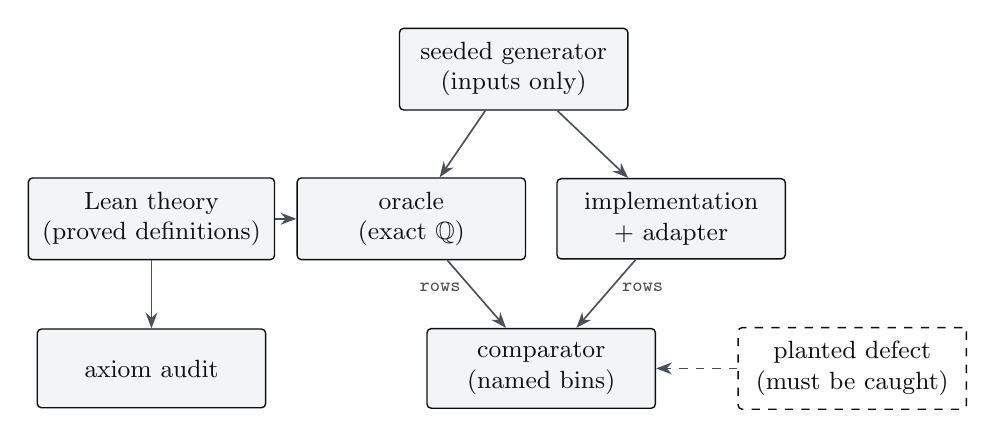
\begin{tikzpicture}[
  box/.style={draw=Ink, line width=0.5pt, fill=Surface, text=Ink, rounded corners=1.5pt,
    align=center, font=\small, inner sep=5pt, minimum height=10mm, minimum width=29mm},
  arr/.style={-{Stealth[length=2mm]}, line width=0.6pt, draw=InkMuted},
  lab/.style={font=\ttfamily\scriptsize, text=InkMuted}]
\node[box] (gen) at (4.6,1.9) {seeded generator\\(inputs only)};
\node[box] (theory) at (0,0) {Lean theory\\(proved definitions)};
\node[box] (oracle) at (3.3,0) {oracle\\(exact $\mathbb{Q}$)};
\node[box] (impl) at (6.6,0) {implementation\\+ adapter};
\node[box] (cmp) at (4.95,-1.9) {comparator\\(named bins)};
\node[box] (audit) at (0,-1.9) {axiom audit};
\node[box, dashed, fill=Background] (planted) at (8.9,-1.9) {planted defect\\(must be caught)};
\draw[arr] (gen) -- (oracle);
\draw[arr] (gen) -- (impl);
\draw[arr] (theory) -- (oracle);
\draw[arr] (theory) -- (audit);
\draw[arr] (oracle) -- node[left, lab, pos=0.4] {rows} (cmp);
\draw[arr] (impl) -- node[right, lab, pos=0.4] {rows} (cmp);
\draw[arr, dashed] (planted) -- (cmp);
\end{tikzpicture}
\caption{The measurement procedure. The generator never computes expected results;
those come only from the oracle.}
\label{fig:harness}
\end{figure}

The procedure follows \texttt{ledger-semantics} (\cref{fig:harness}). A seeded
generator writes case files containing inputs only. It favors the inputs where
implementations are known to have conventions: tied logits, words that are
themselves tokens, and merge tables with several splits of one string. A small
adapter per implementation runs the same cases and prints the oracle's row format.
The comparator places every case in exactly one named bin (agree, diverge, skipped
by either side, or missing), so nothing is dropped silently. Token rows are compared
as strings. Sampler rows require that a zero be matched by a zero and that nonzero
probabilities agree within $10^{-6}$, since llama.cpp stores logits in
\texttt{float32}. Each comparator is observed to fail: a planted defect, an adapter
that glues two tokens or one that inverts temperature, must be detected or the run
fails.

\paragraph{Tie divergences.} An implementation that keeps exactly $k$ tokens breaks
ties in its own order, which need not be the oracle's order by index. Every filter
treats tied tokens alike except for that choice, and tied tokens stay tied through
temperature and renormalization. Such an implementation must therefore agree with
the positional semantics up to a permutation of tied tokens. The harness checks
exactly this: the multiset of (logit, probability) pairs over the kept tokens must
equal that of the oracle's \texttt{q} rows. A divergence that fails this check is
reported as unexplained.

\begin{table}[t]
\centering\small
\caption{Measurements (\texttt{harness/run.sh 600}: four seeds of 600 cases each per
corpus). Lean 4.34.1, Mathlib v4.34.1, \texttt{tokenizers} 0.23.3, \texttt{tiktoken}
0.14.0, llama.cpp commit \texttt{a9d27ac} (2026-10-11).}
\label{tab:results}
\begin{tabularx}{\linewidth}{@{}>{\raggedright\arraybackslash}p{4.6cm}>{\raggedright\arraybackslash}X>{\raggedright\arraybackslash}X@{}}
\toprule
\qpth{Implementation} & \qpth{Compared against} & \qpth{Result}\\
\midrule
HF \texttt{tokenizers}, BPE, defaults & rule-rank BPE (\lean{bpe}) & 13{,}779 / 13{,}779 words identical\\
HF \texttt{tokenizers}, \lean{ignore_merges} & lookup, then rule-rank BPE & 13{,}779 / 13{,}779 identical\\
\texttt{tiktoken} & lookup, then concatenation-rank BPE & 13{,}779 / 13{,}779 identical\\
llama.cpp \lean{top_k}, \lean{top_p}, \lean{min_p}, \texttt{temp}, no ties & tie-keeping filters & 1{,}216 / 1{,}216 chains, $|\Delta p|\le5.1\times10^{-8}$\\
llama.cpp, with ties & tie-keeping, else positional & 939 + 245 / 1{,}184 chains; 0 unexplained\\
Planted defects (tokenizer, sampler) & --- & both detected\\
\bottomrule
\end{tabularx}
\end{table}

\Cref{tab:results} summarizes the results. Two findings came out of the
comparisons. First, \texttt{tiktoken} initially disagreed with the oracle's
concatenation-rank BPE on words that are themselves vocabulary tokens. The
disagreement was a convention, whole-word lookup. Following the
\texttt{ledger-semantics} rule that a divergence is either a defect in the
implementation or a convention the semantics has not yet recorded, we recorded it
as \lean{lookupFirst}, with its own theorems, after which agreement is exact.
Second, on the same random merge tables the two tokenizer libraries disagree with
each other on 439 of 13{,}779 words (3.2\%), and on 279 when Hugging Face uses
\lean{ignore_merges}. The oracle reproduces each library exactly, so every one of
these disagreements is predicted. \Cref{thm:bpeconv} states the condition under which
they cannot occur.

For sampling, llama.cpp agrees with the tie-keeping semantics on every tie-free
chain. On chains with ties, 245 of 1{,}184 diverge, and every one agrees with the
positional semantics up to a permutation of tied tokens. Some of these divergences
cascade: a tie cut by top-$k$ changes the renormalized masses that a later top-$p$
sees. A check that compared kept sets only after the fact would misclassify such
cases. Replaying the convention exactly classifies all of them.

% ===========================================================================
\section{Related work}

\paragraph{Formal methods for machine learning.} Most verification work on neural
networks proves properties of trained models, for example with SMT-based
methods~\cite{katz2017reluplex}. We verify the model-independent algorithms around
the model instead, and connect them to implementations through an oracle. The
denotational method follows Elliott~\cite{elliott2009denotational}. The use of a
proved semantics as a test oracle, the procedure of planted defects, and the
discipline of named skip bins follow \texttt{ledger-semantics}~\cite{ledgersemantics}.
Our category of finite stochastic maps is a special case of Fritz's Markov
categories~\cite{fritz2020markov}.

\paragraph{Tokenization.} Zouhar et al.\ give a formal analysis of BPE as an
optimization problem~\cite{zouhar2023bpe}. Gastaldi et al.\ treat tokenizers as
stochastic maps and study consistency of estimators~\cite{gastaldi2024foundations}.
Vieira et al.\ show how to turn token-level models into character-level
ones~\cite{vieira2024tokens}, which requires exactly the enumeration of
tokenizations we verify. Our no-compression theorem and the agreement criterion
between BPE conventions complement this work at the level of exact identities.

\paragraph{Decoding.} Top-$k$~\cite{fan2018hierarchical}, nucleus~\cite{holtzman2020curious}
and min-$p$~\cite{nguyen2025minp} sampling are usually specified by an algorithm over
sorted arrays, which leaves ties unspecified. \Cref{thm:topk} shows that this gap
cannot be closed by any symmetric rule. Speculative
sampling~\cite{leviathan2023speculative,chen2023speculative} is known to be lossless,
and its acceptance rate is the maximal-coupling bound~\cite{lindvall1992coupling}. Du et
al.\ characterize tightness measure-theoretically~\cite{du2023tight}. We give a
finite-depth statement and an explicit non-tight model.

\paragraph{Attention and inference systems.} Online softmax~\cite{milakov2018online}
underlies FlashAttention~\cite{dao2022flashattention} and its successors, and
KV caching is standard in serving systems~\cite{pope2023scaling,kwon2023vllm}. Our
contribution is the algebraic packaging, a commutative monoid with a free-monoid
homomorphism, and machine-checked proofs over arbitrary exponential characters.
Permutation equivariance of attention without positional encodings is
known~\cite{yun2020universal}.

\paragraph{Masked diffusion.} The time-independence of the optimal denoiser was
observed by Ou et al.~\cite{ou2025absorbing}, in the setting of
D3PM~\cite{austin2021d3pm}, MDLM~\cite{sahoo2024mdlm} and related
models~\cite{shi2024masked,nie2025llada}. We machine-check it, together with the
any-order chain rule and the inexactness of parallel unmasking.

% ===========================================================================
\section{Limitations}

Analysis on the reals enters only through exponential characters, and there is no
measure theory, so sampling and tightness are stated through finite quantities. The
oracle's temperature is restricted to $1/n$, which keeps softmax rational. The
theorems hold for every temperature, but the oracle cannot evaluate an irrational
softmax. Speculative decoding is proved for one drafted token. The sequence version
follows by induction and is not yet formalized. Nothing is proved about
floating-point arithmetic: implementations are compared with exact values within a
stated tolerance. A decision that lies exactly on a floating-point boundary could in
principle diverge, and none occurred in our runs. The diffusion theory covers
absorbing diffusion, not Gaussian diffusion. The chat protocol models tool calling in
its common request-and-result form, not any vendor's specification. The measurements
cover tokenizers and samplers; attention kernels, speculative decoders, chat
renderers and diffusion samplers are evaluated by the oracle but not yet compared
against implementations.

% ===========================================================================
\section{Conclusion}

The inference side of LLMs is small enough to be given a precise meaning and large
enough that its implementations disagree. A machine-checked semantics separates
what is meaning from what is convention. It proves which reorderings, cachings and
tilings are harmless, and it shows that some properties folklore expects, such as
symmetric exact top-$k$, compositional compressing tokenizers and unambiguous plain-text
templates, cannot exist. Connected to an exact oracle, the same definitions become
a test instrument. Every divergence it surfaces is either a defect in an
implementation or a convention that belongs in the semantics.

\paragraph{Availability.} The Lean development, oracle, harness, and recorded
measurement log accompany this paper.

\paragraph{Acknowledgments.} The structure of this work follows
\texttt{ledger-semantics} by John Wiegley. The formalization and harness were
developed with the assistance of an AI system (Claude, Anthropic).

% ===========================================================================
\begin{thebibliography}{99}\small

\bibitem{austin2021d3pm}
J.~Austin, D.~D. Johnson, J.~Ho, D.~Tarlow, and R.~van~den Berg.
\newblock Structured denoising diffusion models in discrete state-spaces.
\newblock In \emph{NeurIPS}, 2021.

\bibitem{chen2023speculative}
C.~Chen, S.~Borgeaud, G.~Irving, J.-B. Lespiau, L.~Sifre, and J.~Jumper.
\newblock Accelerating large language model decoding with speculative sampling.
\newblock arXiv:2302.01318, 2023.

\bibitem{dao2022flashattention}
T.~Dao, D.~Y. Fu, S.~Ermon, A.~Rudra, and C.~R{\'e}.
\newblock {FlashAttention}: Fast and memory-efficient exact attention with {IO}-awareness.
\newblock In \emph{NeurIPS}, 2022.

\bibitem{demoura2021lean4}
L.~de~Moura and S.~Ullrich.
\newblock The {Lean} 4 theorem prover and programming language.
\newblock In \emph{CADE-28}, 2021.

\bibitem{du2023tight}
L.~Du, L.~Torroba~Hennigen, T.~Pimentel, C.~Meister, J.~Eisner, and R.~Cotterell.
\newblock A measure-theoretic characterization of tight language models.
\newblock In \emph{ACL}, 2023.

\bibitem{elliott2009denotational}
C.~Elliott.
\newblock Denotational design with type class morphisms.
\newblock Technical Report 2009-01, LambdaPix, 2009.

\bibitem{fan2018hierarchical}
A.~Fan, M.~Lewis, and Y.~Dauphin.
\newblock Hierarchical neural story generation.
\newblock In \emph{ACL}, 2018.

\bibitem{fritz2020markov}
T.~Fritz.
\newblock A synthetic approach to {Markov} kernels, conditional independence and theorems on sufficient statistics.
\newblock \emph{Advances in Mathematics}, 370, 2020.

\bibitem{gastaldi2024foundations}
J.~L. Gastaldi, J.~Terilla, L.~Malagutti, B.~DuSell, T.~Vieira, and R.~Cotterell.
\newblock The foundations of tokenization: Statistical and computational concerns.
\newblock arXiv:2407.11606, 2024.

\bibitem{greshake2023injection}
K.~Greshake, S.~Abdelnabi, S.~Mishra, C.~Endres, T.~Holz, and M.~Fritz.
\newblock Not what you've signed up for: Compromising real-world {LLM}-integrated applications with indirect prompt injection.
\newblock In \emph{AISec}, 2023.

\bibitem{holtzman2020curious}
A.~Holtzman, J.~Buys, L.~Du, M.~Forbes, and Y.~Choi.
\newblock The curious case of neural text degeneration.
\newblock In \emph{ICLR}, 2020.

\bibitem{katz2017reluplex}
G.~Katz, C.~Barrett, D.~L. Dill, K.~Julian, and M.~J. Kochenderfer.
\newblock Reluplex: An efficient {SMT} solver for verifying deep neural networks.
\newblock In \emph{CAV}, 2017.

\bibitem{kwon2023vllm}
W.~Kwon, Z.~Li, S.~Zhuang, Y.~Sheng, L.~Zheng, C.~H. Yu, J.~E. Gonzalez, H.~Zhang, and I.~Stoica.
\newblock Efficient memory management for large language model serving with {PagedAttention}.
\newblock In \emph{SOSP}, 2023.

\bibitem{ledgersemantics}
J.~Wiegley.
\newblock ledger-semantics: Mathematical semantics of {Ledger}, the double-entry accounting tool.
\newblock \url{https://github.com/ledger/ledger-semantics}, 2026.

\bibitem{leviathan2023speculative}
Y.~Leviathan, M.~Kalman, and Y.~Matias.
\newblock Fast inference from transformers via speculative decoding.
\newblock In \emph{ICML}, 2023.

\bibitem{lindvall1992coupling}
T.~Lindvall.
\newblock \emph{Lectures on the Coupling Method}.
\newblock Wiley, 1992.

\bibitem{liu2023ring}
H.~Liu, M.~Zaharia, and P.~Abbeel.
\newblock Ring attention with blockwise transformers for near-infinite context.
\newblock arXiv:2310.01889, 2023.

\bibitem{mathlib2020}
The mathlib Community.
\newblock The {Lean} mathematical library.
\newblock In \emph{CPP}, 2020.

\bibitem{milakov2018online}
M.~Milakov and N.~Gimelshein.
\newblock Online normalizer calculation for softmax.
\newblock arXiv:1805.02867, 2018.

\bibitem{nguyen2025minp}
M.~N. Nguyen, A.~Baker, C.~Neo, A.~Roush, A.~Kirsch, and R.~Shwartz-Ziv.
\newblock Turning up the heat: Min-p sampling for creative and coherent {LLM} outputs.
\newblock In \emph{ICLR}, 2025.

\bibitem{nie2025llada}
S.~Nie, F.~Zhu, Z.~You, X.~Zhang, J.~Ou, J.~Hu, J.~Zhou, Y.~Lin, J.-R. Wen, and C.~Li.
\newblock Large language diffusion models.
\newblock arXiv:2502.09992, 2025.

\bibitem{ou2025absorbing}
J.~Ou, S.~Nie, K.~Xue, F.~Zhu, J.~Sun, Z.~Li, and C.~Li.
\newblock Your absorbing discrete diffusion secretly models the conditional distributions of clean data.
\newblock In \emph{ICLR}, 2025.

\bibitem{pope2023scaling}
R.~Pope, S.~Douglas, A.~Chowdhery, J.~Devlin, J.~Bradbury, J.~Heek, K.~Xiao, S.~Agrawal, and J.~Dean.
\newblock Efficiently scaling transformer inference.
\newblock In \emph{MLSys}, 2023.

\bibitem{rabe2021selfattention}
M.~N. Rabe and C.~Staats.
\newblock Self-attention does not need {$O(n^2)$} memory.
\newblock arXiv:2112.05682, 2021.

\bibitem{radford2019gpt2}
A.~Radford, J.~Wu, R.~Child, D.~Luan, D.~Amodei, and I.~Sutskever.
\newblock Language models are unsupervised multitask learners.
\newblock OpenAI technical report, 2019.

\bibitem{sahoo2024mdlm}
S.~S. Sahoo, M.~Arriola, Y.~Schiff, A.~Gokaslan, E.~Marroquin, J.~T. Chiu, A.~Rush, and V.~Kuleshov.
\newblock Simple and effective masked diffusion language models.
\newblock In \emph{NeurIPS}, 2024.

\bibitem{sennrich2016bpe}
R.~Sennrich, B.~Haddow, and A.~Birch.
\newblock Neural machine translation of rare words with subword units.
\newblock In \emph{ACL}, 2016.

\bibitem{shi2024masked}
J.~Shi, K.~Han, Z.~Wang, A.~Doucet, and M.~K. Titsias.
\newblock Simplified and generalized masked diffusion for discrete data.
\newblock In \emph{NeurIPS}, 2024.

\bibitem{vieira2024tokens}
T.~Vieira, B.~LeBrun, M.~Giulianelli, J.~L. Gastaldi, B.~DuSell, J.~Terilla, T.~J. O'Donnell, and R.~Cotterell.
\newblock From language models over tokens to language models over characters.
\newblock arXiv:2412.03719, 2024.

\bibitem{wolf2020transformers}
T.~Wolf et~al.
\newblock Transformers: State-of-the-art natural language processing.
\newblock In \emph{EMNLP: System Demonstrations}, 2020.

\bibitem{xiao2024sinks}
G.~Xiao, Y.~Tian, B.~Chen, S.~Han, and M.~Lewis.
\newblock Efficient streaming language models with attention sinks.
\newblock In \emph{ICLR}, 2024.

\bibitem{yun2020universal}
C.~Yun, S.~Bhojanapalli, A.~S. Rawat, S.~J. Reddi, and S.~Kumar.
\newblock Are transformers universal approximators of sequence-to-sequence functions?
\newblock In \emph{ICLR}, 2020.

\bibitem{zouhar2023bpe}
V.~Zouhar, C.~Meister, J.~L. Gastaldi, L.~Du, T.~Vieira, M.~Sachan, and R.~Cotterell.
\newblock A formal perspective on byte-pair encoding.
\newblock In \emph{Findings of ACL}, 2023.

\end{thebibliography}

\end{document}
"

\usepackage[a4paper,textwidth=15.4cm,textheight=23.6cm,top=3.0cm,headsep=0.9cm,footskip=1.2cm]{geometry}
\usepackage{amsmath,amssymb,amsthm,mathtools}
\usepackage{fontspec}
\usepackage{booktabs,tabularx,array}
\usepackage[protrusion=true,expansion=false]{microtype}
\usepackage[table]{xcolor}
\usepackage{graphicx}
\usepackage{fvextra}
\usepackage{enumitem}
\usepackage{caption}
\usepackage{titlesec}
\usepackage{fancyhdr}
\usepackage[most]{tcolorbox}
\usepackage{tikz}
\usetikzlibrary{arrows.meta}
\usepackage{hyperref}
\usepackage[nameinlink,capitalise]{cleveref}

% ---------------------------------------------------------------------------
%  Colour tokens
% ---------------------------------------------------------------------------
% Neutral foundation. Ink and Background invert between the two editions.
\ifqptdark
  \definecolor{Background}{HTML}{0B0C0E}
  \definecolor{Surface}{HTML}{16181B}
  \definecolor{Border}{HTML}{2B2E33}
  \definecolor{Ink}{HTML}{EDEEF0}
  \definecolor{InkMuted}{HTML}{A9AEB6}
  \definecolor{InkFaint}{HTML}{5A5F67}   % decoration only, never meaningful text
\else
  \definecolor{Background}{HTML}{FFFFFF}
  \definecolor{Surface}{HTML}{F3F4F5}
  \definecolor{Border}{HTML}{DADDE1}
  \definecolor{Ink}{HTML}{0E0F11}
  \definecolor{InkMuted}{HTML}{4B4F57}
  \definecolor{InkFaint}{HTML}{A3A7AE}   % decoration only, never meaningful text
\fi
% Paradigm colours: fixed in both editions, semantic only.
\definecolor{Quantum}{HTML}{5BAD1E}
\definecolor{Photonic}{HTML}{F0AB00}
\definecolor{Thermodynamic}{HTML}{E8690A}
\definecolor{Ternary}{HTML}{8A8A8A}
\definecolor{Bio}{HTML}{1AAB7C}

\ifqptdark\pagecolor{Background}\fi

% ---------------------------------------------------------------------------
%  Typography
% ---------------------------------------------------------------------------
\setmainfont{Inter}[
  Path=fonts/, Extension=.otf, Scale=0.94,
  UprightFont=*-Regular, ItalicFont=*-Italic,
  BoldFont=*-SemiBold, BoldItalicFont=*-SemiBoldItalic]
\setmonofont{IBMPlexMono}[
  Path=fonts/, Extension=.ttf, Scale=MatchLowercase,
  UprightFont=*-Regular, ItalicFont=*-Italic, BoldFont=*-SemiBold]
\newfontfamily\qptdisplay{SpaceGrotesk}[
  Path=fonts/, Extension=.otf, UprightFont=*-Medium, BoldFont=*-Bold]
\newfontfamily\qptdisplaylight{SpaceGrotesk}[
  Path=fonts/, Extension=.otf, UprightFont=*-Regular]
\newfontfamily\qptlabelfont{IBMPlexMono}[
  Path=fonts/, Extension=.ttf, Scale=MatchLowercase, UprightFont=*-Medium,
  LetterSpace=6]
\setsansfont{Inter}[
  Path=fonts/, Extension=.otf, Scale=0.94,
  UprightFont=*-Regular, ItalicFont=*-Italic,
  BoldFont=*-SemiBold, BoldItalicFont=*-SemiBoldItalic]
\linespread{1.16}
\setlength{\emergencystretch}{2.5em}
\AtBeginDocument{\raggedright\setlength{\parindent}{0pt}}
\setlength{\parindent}{0pt}
\setlength{\parskip}{0.55em}

% A label: IBM Plex Mono, upper case, tracked.
\newcommand{\qptlabel}[1]{{\qptlabelfont\footnotesize\MakeUppercase{#1}}}
% Technical names (Lean declarations, files) in IBM Plex Mono.
\newcommand{\lean}[1]{\texttt{\detokenize{#1}}}
\newcommand{\leanref}[1]{\par\smallskip\noindent
  {\ttfamily\footnotesize\upshape\raggedright\color{InkMuted}LEAN\enspace #1\par}}

% Ink is the normal colour everywhere, including floats, heads and footnotes.
\makeatletter
\AtBeginDocument{\color{Ink}\global\let\default@color\current@color}
\makeatother

% ---------------------------------------------------------------------------
%  Mathematical notation
% ---------------------------------------------------------------------------
\newcommand{\K}{\Bbbk}
\newcommand{\Dist}{\mathrm{Dist}}
\newcommand{\restr}[2]{#1|_{#2}}
\newcommand{\topk}{\mathrm{TopK}}
\newcommand{\topp}{\mathrm{TopP}}
\newcommand{\minp}{\mathrm{MinP}}
\newcommand{\sharpen}{\mathrm{sharpen}}
\newcommand{\abv}{\mathrm{above}}
\newcommand{\tv}{\mathrm{tv}}
\newcommand{\dec}{\mathrm{dec}}
\newcommand{\enc}{\mathrm{enc}}
\newcommand{\softmax}{\mathrm{softmax}}
\newcommand{\attend}{\mathrm{attend}}
\newcommand{\Iv}[1]{[\![#1]\!]}
\newcommand{\Mask}{\bot}

% ---------------------------------------------------------------------------
%  Headings: section numbers as labels, titles in Space Grotesk
% ---------------------------------------------------------------------------
\makeatletter
\newcommand{\qptsecnum}[1]{{\qptlabelfont\small\color{InkMuted}\two@digits{#1}}}
\makeatother
\titleformat{\section}
  {\qptdisplay\fontsize{14.5}{18}\selectfont\color{Ink}}
  {\qptsecnum{\value{section}}}{0.9em}{}
\titleformat{name=\section,numberless}
  {\qptdisplay\fontsize{14.5}{18}\selectfont\color{Ink}}{}{0pt}{}
\titlespacing*{\section}{0pt}{1.9em}{0.7em}
\titleformat{\paragraph}[runin]
  {\qptdisplay\normalsize\color{Ink}}{}{0pt}{}
\titlespacing*{\paragraph}{0pt}{0.9em}{0.6em}

% ---------------------------------------------------------------------------
%  Statements
% ---------------------------------------------------------------------------
\newtheoremstyle{qpt}
  {0.9em}{0.9em}
  {\normalfont}{}
  {\qptlabelfont\footnotesize}{}
  {\newline}
  {\MakeUppercase{\thmname{#1}\thmnumber{~#2}}%
   \thmnote{\enspace{\qptdisplay\normalsize\color{Ink}#3}}}
\theoremstyle{qpt}
\newtheorem{theorem}{Theorem}
\newtheorem{proposition}[theorem]{Proposition}
\newtheorem{corollary}[theorem]{Corollary}
\newtheorem{lemma}[theorem]{Lemma}
\newtheorem{definition}[theorem]{Definition}
\newtheorem{remark}[theorem]{Remark}

% Proofs: a tracked label and a neutral end mark.
\makeatletter
\renewcommand{\qedsymbol}{{\color{InkMuted}\rule{0.5em}{0.5em}}}
\renewenvironment{proof}[1][Proof]{\par\pushQED{\qed}\normalfont\topsep0.5em\relax
  \trivlist\item[\hskip\labelsep\qptlabel{#1}\hspace{0.6em}]\ignorespaces}
  {\popQED\endtrivlist\@endpefalse}
\makeatother

% ---------------------------------------------------------------------------
%  Code: IBM Plex Mono on a neutral surface, with a hairline on the left
% ---------------------------------------------------------------------------
\tcbset{colupper=Ink, collower=Ink}
\tcbset{qptcode/.style={enhanced, colback=Surface, colframe=Surface,
  boxrule=0pt, arc=0pt, left=9pt, right=8pt, top=5pt, bottom=5pt,
  borderline west={1.2pt}{0pt}{InkFaint}, before skip=0.7em, after skip=0.7em}}
\newenvironment{leancode}
  {\VerbatimEnvironment\begin{tcolorbox}[qptcode]%
   \begin{Verbatim}[fontsize=\small,commandchars=\\\{\},
     codes={\catcode`\$=3\catcode`\^=7},formatcom=\color{Ink}]}
  {\end{Verbatim}\end{tcolorbox}}
\newenvironment{casecode}
  {\VerbatimEnvironment\begin{tcolorbox}[qptcode,before skip=0pt,after skip=0pt]%
   \begin{Verbatim}[fontsize=\footnotesize,formatcom=\color{Ink}]}
  {\end{Verbatim}\end{tcolorbox}}

% ---------------------------------------------------------------------------
%  Floats, tables, captions
% ---------------------------------------------------------------------------
\DeclareCaptionLabelFormat{qpt}{\qptlabel{#1~#2}}
\DeclareCaptionLabelSeparator{qptsep}{\quad}
\captionsetup{labelformat=qpt, labelsep=qptsep, font={small,color=Ink},
  justification=raggedright, singlelinecheck=false, skip=6pt}
\newcommand{\qpth}[1]{\qptlabel{#1}}
\arrayrulecolor{Ink}
\setlength{\heavyrulewidth}{0.7pt}
\setlength{\lightrulewidth}{0.35pt}
\renewcommand{\arraystretch}{1.22}

% ---------------------------------------------------------------------------
%  Running heads
% ---------------------------------------------------------------------------
\pagestyle{fancy}
\fancyhf{}
\fancyhead[L]{{\color{Ink}\qptlabel{Machine-checked semantics of LLM inference}}}
\fancyhead[R]{{\color{Ink}\qptlabel{D. Arango Sohm}}}
\fancyfoot[R]{{\ttfamily\small\color{InkMuted}\thepage}}
\renewcommand{\headrule}{{\color{Border}\hrule height 0.4pt}\vspace{-0.4pt}}
\renewcommand{\headrulewidth}{0.4pt}
\fancypagestyle{qptfirst}{\fancyhf{}%
  \fancyfoot[R]{{\ttfamily\small\color{InkMuted}\thepage}}%
  \renewcommand{\headrulewidth}{0pt}\renewcommand{\headrule}{}}

% ---------------------------------------------------------------------------
%  Links and references: neutral, never accent-coloured text
% ---------------------------------------------------------------------------
\hypersetup{colorlinks=true, linkcolor=Ink, citecolor=Ink, urlcolor=Ink,
  pdftitle={A Machine-Checked Semantics of LLM Inference},
  pdfauthor={Daniel Arango Sohm},
  pdfsubject={Formal semantics of large language model inference in Lean 4},
  pdfkeywords={Lean 4, Mathlib, formal verification, LLM inference, sampling,
    tokenization, attention, speculative decoding, diffusion language models}}
\makeatletter
\renewcommand{\@biblabel}[1]{{\ttfamily\color{InkMuted}[#1]}}
\renewcommand{\@cite}[2]{{\ttfamily[#1\if@tempswa, #2\fi]}}
\makeatother
\renewcommand{\refname}{References}

\setlist{itemsep=2pt, topsep=4pt}
\setlist[itemize]{label={\color{InkMuted}\textbullet}}

\begin{document}
\thispagestyle{qptfirst}

% ----------------------------------------------------------------- masthead
\noindent
\begin{minipage}[c]{0.5\linewidth}
  \includegraphics[height=1.9cm]{qpt-logo.png}
\end{minipage}%
\begin{minipage}[c]{0.5\linewidth}\raggedleft
  \qptlabel{Preprint}\\[2pt]
  \qptlabel{October 2026}
\end{minipage}

\vspace{1.6em}
{\color{Border}\rule{\linewidth}{0.4pt}}
\vspace{1.1em}

{\qptdisplay\fontsize{25}{29.5}\selectfont\color{Ink}
A Machine-Checked Semantics\\ of LLM Inference\par}
\vspace{0.55em}
{\qptdisplaylight\fontsize{13}{17}\selectfont\color{InkMuted}
Sampling, Attention, Tokenization, Chat, Decoding,\\ and Diffusion in Lean~4\par}

\vspace{1.5em}
{\large\bfseries Daniel Arango Sohm}\par
\vspace{0.15em}
{\color{InkMuted}Universidad EAFIT, Medellín, Colombia\\
Former member of the QPT team}\par

\vspace{1.4em}
% ----------------------------------------------------------------- abstract
\begin{tcolorbox}[enhanced, colback=Surface, colframe=Surface, colupper=Ink, boxrule=0pt,
  arc=0pt, left=12pt, right=12pt, top=9pt, bottom=10pt]
\qptlabel{Abstract}\par\vspace{0.35em}
{\small
The inference side of a large language model is a stack of small algorithms:
tokenizers, attention kernels, key--value caches, sampling filters, speculative
decoders, chat templates, and diffusion samplers. Each has several independent
implementations, and those implementations are usually tested against one another
rather than against a definition. We give these components a single mathematical
semantics, formalized in Lean~4 against Mathlib. The development comprises about
4{,}600 lines and 270 named theorems, and every declaration depends only on Lean's
three standard axioms. It proves the exact algebra of sampling filters, the
losslessness and optimality of speculative sampling, and the correctness of
key--value caching and of FlashAttention-style online softmax as a commutative
monoid. It proves that byte-pair encoding is lossless under every merge priority,
together with a decidable criterion for when the Hugging Face and \texttt{tiktoken}
conventions agree, a protocol checker for tool calls, and the time-independence of
the masked-diffusion denoiser. It also proves six negative results. No sampling
rule that treats tokens symmetrically can always keep exactly $k$ tokens. No
tokenizer that compresses can respect concatenation. Every chat template that writes
its role markers in the content alphabet is ambiguous. No transformer without
positional information can copy a fixed position. An autoregressive model need not
define a distribution over strings. Parallel unmasking in diffusion is inexact.
From the same definitions we build an executable oracle that evaluates test cases in
exact rational arithmetic, and a harness that measures implementations against it.
On 2{,}400 random merge tables, Hugging Face \texttt{tokenizers} and
\texttt{tiktoken} each agree with the oracle on all 13{,}779 test words, while
disagreeing with each other on 3.2\% of them. On 2{,}400 random sampler chains,
every divergence of llama.cpp from the tie-keeping semantics is accounted for
exactly by the positional semantics that the impossibility theorem forces.
\par}
\end{tcolorbox}

\vspace{0.3em}
\noindent\qptlabel{Keywords}\enspace{\small Lean~4 · Mathlib · formal verification ·
LLM inference · sampling · tokenization · attention · speculative decoding ·
diffusion language models}

\vspace{0.4em}
{\color{Border}\rule{\linewidth}{0.4pt}}

% ===========================================================================
\section{Introduction}

A deployed language model is a function from parameters and a context to a
distribution over tokens. Turning that distribution into text requires more
machinery. A tokenizer maps strings to token sequences. Attention kernels compute
the model's reads over a cached context. A chain of sampling filters reshapes the
next-token distribution. A speculative decoder may verify drafted tokens, a chat
template linearizes a conversation, and a diffusion sampler may unmask several
positions at once. Each of these components exists in many implementations, such as
Hugging Face \texttt{transformers} and \texttt{tokenizers}~\cite{wolf2020transformers},
\texttt{tiktoken}, vLLM~\cite{kwon2023vllm}, and llama.cpp. Their tests mostly
compare one implementation with another, or with remembered behavior.

This paper follows a different discipline, \emph{denotational design}~\cite{elliott2009denotational}.
One first says precisely what a thing means, then requires every operation to
preserve that meaning, and lets the implementation be whatever the equations force
it to be. The approach is that of \texttt{ledger-semantics}~\cite{ledgersemantics},
which formalizes double-entry accounting in Lean and uses the result as a test oracle
for the C++ Ledger program. We apply it to LLM inference. A sampling filter means
conditioning a distribution on a set. A KV-cached decoder means causal attention over
the whole prefix. A FlashAttention kernel means a softmax-weighted average. A chat
template means an injective encoding of a transcript. The theorems state when an
implementation preserves that meaning, and several of them state that no
implementation can.

\paragraph{Contributions.}
\begin{itemize}[leftmargin=*,itemsep=2pt]
\item A Lean~4 formalization against Mathlib~\cite{mathlib2020,demoura2021lean4}
  of sampling, speculative decoding, softmax and attention, tokenization, chat
  transcripts, autoregressive decoding, and masked diffusion
  (\cref{sec:foundations,sec:sampling,sec:spec,sec:attention,sec:tokenization,sec:chat,sec:decoding,sec:diffusion}).
  All definitions are stated over an arbitrary linearly ordered field, so one proof
  covers the real numbers of the literature and the exact rationals of the oracle.
\item Positive results in a common framework. They include the algebra of
  sampling filters, the optimality of speculative sampling, an online-softmax
  commutative monoid, a generic correctness theorem for BPE with a decidable
  agreement criterion between the two conventions in use, a protocol checker for
  tool calls, and the any-order chain rule for masked diffusion.
\item Six negative results that explain design constraints visible across
  implementations (\cref{sec:negative}).
\item An executable oracle that evaluates case files under the proved
  definitions in exact arithmetic, and a measurement of Hugging Face
  \texttt{tokenizers}, \texttt{tiktoken}, and llama.cpp against it (\cref{sec:oracle,sec:measure}).
\end{itemize}

Several of the positive results are known: losslessness of speculative
sampling~\cite{leviathan2023speculative,chen2023speculative}, correctness of online
softmax~\cite{milakov2018online,dao2022flashattention}, time-independence of the
absorbing-diffusion posterior~\cite{ou2025absorbing}, and the role of permutation
equivariance~\cite{yun2020universal}. Our contribution for these is a machine-checked
statement in one framework, connected to an oracle. To our knowledge the
following are not stated elsewhere in the form given here: the impossibility of
symmetric exact top-$k$ and nucleus selection, the no-compression theorem for
homomorphic tokenizers, the ambiguity of every in-band chat template, and the
decidable agreement criterion between merge-rule and concatenation-rank BPE.

% ===========================================================================
\section{Method and trust base}\label{sec:method}

The development is a Lean~4 library (Lean 4.34.1, Mathlib v4.34.1) of eleven
theory modules and two executable modules (\cref{tab:modules}). It is built with
warnings promoted to errors, so an unproved theorem (\lean{sorry}) fails the build.
A separate audit program walks every declaration in the library, 853 in all, and
fails unless each depends only on propositional extensionality, the axiom of choice,
and quotient soundness. The audit has been observed to fail: a planted proof by
\lean{native_decide}, which introduces an auxiliary axiom trusting compiled code, is
rejected. The warnings-as-errors build alone does not catch it. Concrete
counterexamples are therefore proved by \lean{decide}, whose certificate the kernel
checks by evaluation.

\begin{table}[t]
\centering\small
\caption{Modules of the development. Lines and named theorems and lemmas per module.}
\label{tab:modules}
\begin{tabularx}{\linewidth}{@{}l>{\raggedright\arraybackslash}X>{\ttfamily}r>{\ttfamily}r@{}}
\toprule
\qpth{Module} & \qpth{Content} & \qpth{Lines} & \qpth{Thms} \\
\midrule
\lean{Dist} & finite distributions, conditioning, total variation, $\mathsf{FinStoch}$ & 383 & 34\\
\lean{Sampling} & top-$k$, top-$p$, min-$p$, temperature, ties, inverse CDF & 732 & 46\\
\lean{Counterexamples} & kernel-checked failures of sampler laws & 52 & 4\\
\lean{Speculative} & speculative sampling, couplings & 194 & 17\\
\lean{Softmax} & exponential characters, masking, temperature & 220 & 23\\
\lean{Attention} & equivariance, causality, KV cache, online softmax & 573 & 38\\
\lean{Real} & $\exp$ as a character; textbook restatements & 51 & 4\\
\lean{Tokenization} & free-monoid decoding, BPE conventions, enumeration & 860 & 49\\
\lean{Chat} & tool-call protocol, rendering & 440 & 21\\
\lean{Decoding} & mass conservation, tightness, greedy decoding & 245 & 15\\
\lean{Diffusion} & masked diffusion, posterior, chain rule & 379 & 18\\
\lean{Oracle}, \lean{Driver} & case parsing and exact evaluation & 465 & 1\\
\midrule
Total & & 4{,}594 & 270\\
\bottomrule
\end{tabularx}
\end{table}

\paragraph{Numbers.} Every probability lives in an arbitrary field $\K$ with a
compatible linear order (\lean{[Field K] [LinearOrder K] [IsStrictOrderedRing K]}).
The oracle instantiates $\K=\mathbb{Q}$, so its arithmetic is exact. The analytic
statements instantiate $\K=\mathbb{R}$. No measure theory is used. Sampling is made
precise through interval statements (\cref{thm:invcdf}), and tightness through
masses at finite depth (\cref{sec:decoding}).

% ===========================================================================
\section{Foundations}\label{sec:foundations}

\begin{definition}[Finite distribution]
For a finite type $\alpha$, $\Dist_\K(\alpha)$ is the type of functions
$p:\alpha\to\K$ with $p(a)\ge 0$ for all $a$ and $\sum_a p(a)=1$.
\leanref{\lean{Dist}}
\end{definition}

\begin{leancode}
structure Dist ($\K$ : Type u) [Field $\K$] [LinearOrder $\K$] [IsStrictOrderedRing $\K$]
    ($\alpha$ : Type v) [Fintype $\alpha$] where
  prob : $\alpha$ $\to$ $\K$
  nonneg : $\forall$ a, 0 $\le$ prob a
  sum_eq_one : $\sum$ a, prob a = 1
\end{leancode}

The single operation through which masks, filters and grammar constraints act is
conditioning. For $S\subseteq\alpha$ with $p(S)>0$, write
$\restr{p}{S}(a)=\Iv{a\in S}\,p(a)/p(S)$ (\lean{Dist.restrict}).

\begin{lemma}[Conditioning]\label{lem:restrict}
$\restr{(\restr{p}{S})}{T}=\restr{p}{S\cap T}$ whenever the masses involved are
positive. Moreover $\restr{p}{S}=\restr{p}{S'}$ whenever $S$ and $S'$ contain the same
outcomes of positive probability.
\leanref{\lean{restrict_restrict}, \lean{restrict_congr}}
\end{lemma}

The finite distribution monad (point masses and \lean{bind}) satisfies the monad
laws. Finite types and stochastic maps $\alpha\to\Dist_\K(\beta)$ form a category
$\mathsf{FinStoch}_\K$, given as an instance of Mathlib's \lean{Category} whose
composition is Kleisli composition (\lean{FinStoch.category}). Total variation is
$\tv(p,q)=\sum_a\max(0,p(a)-q(a))$. We prove
$\tv(p,q)=\tfrac12\sum_a|p(a)-q(a)|$, $\sum_a\min(p(a),q(a))=1-\tv(p,q)$, and
$\tv(p,q)=0\iff p=q$.

% ===========================================================================
\section{Sampling}\label{sec:sampling}

Let $V$ be a finite vocabulary and $p:V\to\K$. Write
$\abv_p(v)=\{u: p(v)<p(u)\}$ for the tokens strictly preferred to $v$. The three
standard filters keep the sets
\begin{gather*}
\topk_k(p)=\{v: |\abv_p(v)|<k\},\qquad
\minp_m(p)=\{v:\forall u,\; m\,p(u)\le p(v)\},\\
\topp_P(p)=\Bigl\{v: \textstyle\sum_{u\in\abv_p(v)}p(u)<P\Bigr\},
\end{gather*}
and the filtered distribution is the conditioning $\restr{p}{S}$ on the kept set
$S$. For distinct probabilities, $\topp_P$ is the usual rule ``sort in descending
order and keep the shortest prefix whose mass reaches $P$''. With ties, all three
keep every tied token. Temperature $1/n$ is
$\sharpen_n(p)(v)=p(v)^n/\sum_u p(u)^n$, which stays inside $\mathbb{Q}$. In
\cref{sec:attention} we show that it equals $\softmax(n\cdot z)$ when
$p=\softmax(z)$. Every kept set contains a most probable token, provided $k\ge1$,
$P>0$ and $m\le1$, so no filter can produce an empty distribution.

\begin{theorem}[Sampler algebra]\label{thm:algebra}
For $k,k'\ge1$, $m,m'\le1$ and $n\ge1$, and writing filters in the order they are
applied,
\begin{enumerate}[label=(\roman*),itemsep=1pt]
\item top-$k$ then top-$k'$ equals top-$\min(k,k')$;
\item min-$m$ then min-$m'$ equals min-$\max(m,m')$; in particular both filters are idempotent;
\item top-$k$ and min-$m$ commute;
\item top-$k$ and temperature $1/n$ commute.
\end{enumerate}
\leanref{\lean{topK_topK}, \lean{minP_minP}, \lean{topK_minP_comm}, \lean{topK_sharpen_comm}}
\end{theorem}

\begin{proof}[Proof sketch]
All three kept sets are \emph{upward closed}: if $v$ is kept and $p(v)<p(u)$, then
$u$ is kept. Conditioning on an upward-closed set $S$ leaves $\abv(v)$ unchanged for
$v\in S$ (\lean{above_restrict}), and min-$p$ is insensitive to conditioning on a set
that contains a maximizer (\lean{minP_restrict_iff}). Each identity then reduces,
through \cref{lem:restrict}, to an equality of kept sets. For (iv), $x\mapsto x^n$
is strictly increasing on $[0,\infty)$, and top-$k$ depends only on the order of the
scores (\lean{topKSet_congr}).
\end{proof}

The laws one might expect beyond \cref{thm:algebra} are false. With
$p_0=(\tfrac12,\tfrac3{10},\tfrac15)$, the kernel evaluates the following
(\lean{Counterexamples}).

\begin{proposition}[Failed laws]\label{prop:counter}
\leavevmode\vspace{-0.5\baselineskip}
\begin{enumerate}[label=(\roman*),itemsep=1pt]
\item Top-$p$ is not idempotent: one pass of $\topp_{3/5}$ gives token~1 the probability $\tfrac38$, and a second pass gives it~$0$.
\item Top-$p$ does not commute with top-$k$: top-$p$ then top-2 leaves token~1 at $\tfrac38$, while top-2 then top-$p$ removes it.
\item Top-$p$ does not commute with temperature $\tfrac12$: token~1 ends at $\tfrac9{34}$ in one order and at $0$ in the other.
\item Min-$p$ ($m=\tfrac12$) does not commute with temperature $\tfrac12$, with the same numbers.
\end{enumerate}
\end{proposition}

A sampler chain may therefore reorder top-$k$, min-$p$ and temperature only as
\cref{thm:algebra} allows, and may not move top-$p$ at all.

\paragraph{Ties.} Implementations differ on ties, and the difference is forced.
Call a selection rule $\mathrm{sel}:(V\to\K)\to\mathcal{P}(V)$ \emph{equivariant} if
$\mathrm{sel}(p\circ\sigma^{-1})=\sigma[\mathrm{sel}(p)]$ for every permutation
$\sigma$ of $V$, that is, if relabeling the tokens relabels the output.

\begin{theorem}[No symmetric exact top-$k$]\label{thm:topk}
Let $0<k<|V|$. No equivariant selection rule satisfies $|\mathrm{sel}(p)|=k$ for
every distribution $p$.
\leanref{\lean{no_equivariant_exact_topK}}
\end{theorem}
\begin{proof}
On the uniform distribution $u$ we have $u\circ\sigma^{-1}=u$ for every $\sigma$, so
$\mathrm{sel}(u)$ is invariant under all permutations. If it contains some $v$, then
for any $w$ the transposition $(v\,w)$ maps $v$ to $w$, so it contains $w$ too.
Hence $\mathrm{sel}(u)$ is either empty or all of $V$, and neither has $k$ elements.
\end{proof}

\begin{leancode}
theorem no_equivariant_exact_topK [DecidableEq V] \char123{}k : $\mathbb{N}$\char125{}
    (hk0 : 0 < k) (hkn : k < Fintype.card V)
    (sel : (V $\to$ $\K$) $\to$ Finset V) (hsel : Equivariant sel) :
    $\neg$ $\forall$ d : Dist $\K$ V, (sel d.prob).card = k
\end{leancode}

\begin{theorem}[No symmetric smallest nucleus]
Let $V$ be nonempty and $0<P\le1-1/|V|$. No equivariant rule returns, for every
distribution, a set of minimum cardinality among those of mass at least~$P$.
\leanref{\lean{no_equivariant_exact_nucleus}}
\end{theorem}

The tie-keeping filters are equivariant (\lean{topKSet_equivariant}). The other
option is to break ties by position. Define $u\prec_p v$ if $p(u)>p(v)$, or if
$p(u)=p(v)$ and $u<v$, and let the positional filters count predecessors under
$\prec_p$ instead of $\abv_p$ (\lean{Dist.topKPos}, \lean{Dist.topPPos}).

\begin{theorem}[Positional tie-breaking]
Positional top-$k$ keeps exactly $\min(k,|V|)$ tokens. If $p$ is injective, the
positional and tie-keeping filters coincide. For $0<k<|V|$, positional top-$k$ is
not equivariant.
\leanref{\lean{card_topKPosSet}, \lean{topKPosSet_eq_of_injective}, \lean{topPPosSet_eq_of_injective}, \lean{topKPosSet_not_equivariant}}
\end{theorem}

An implementation must therefore choose between keeping exactly $k$ tokens and
treating tokens symmetrically. Hugging Face \texttt{transformers} (read from the
source of version 5.19.0) keeps ties in top-$k$, since it removes only scores
strictly below the $k$-th largest, but breaks them by sort position in top-$p$.
llama.cpp breaks ties by position in both, as measured in \cref{sec:measure}.

\begin{theorem}[Inverse-CDF sampling]\label{thm:invcdf}
Let $F(i)=\sum_{j<i}p(j)$ on $V=\{0,\dots,n-1\}$ and let $\iota(u)$ be the least $i$
with $u<F(i+1)$. For $0\le u<1$, $\iota(u)=i\iff F(i)\le u<F(i+1)$, and
$F(i+1)-F(i)=p(i)$. A uniform $u$ therefore selects $i$ with probability $p(i)$.
\leanref{\lean{invCdf_eq_iff}, \lean{cdf_interval_length}}
\end{theorem}

% ===========================================================================
\section{Speculative decoding}\label{sec:spec}

A draft model proposes $x\sim q$. The target, with distribution $p$, accepts with
probability $a(x)=\min(1,p(x)/q(x))$, and on rejection a token is drawn from the
residual $r=(p-q)^+/\tv(p,q)$~\cite{leviathan2023speculative,chen2023speculative}.
We define the joint law of (draft, emitted token) exactly as the algorithm runs,
\[
\pi(x,y)=q(x)\bigl(a(x)\,\Iv{y=x}+(1-a(x))\,r(y)\bigr).
\]

\begin{theorem}[Speculative sampling]
\leavevmode\vspace{-0.5\baselineskip}
\begin{enumerate}[label=(\roman*),itemsep=1pt]
\item The draft has law $q$: $\sum_y\pi(x,y)=q(x)$.
\item \emph{Losslessness}: the emitted token has law $p$: $\sum_x\pi(x,y)=p(y)$.
\item The acceptance probability is $\sum_x q(x)a(x)=1-\tv(p,q)$, and the emitted token equals the draft with the same probability.
\item \emph{Optimality}: every coupling $\gamma$ of $q$ and $p$ has $\sum_x\gamma(x,x)\le1-\tv(p,q)$.
\end{enumerate}
\leanref{\lean{specJoint_fst}, \lean{specJoint_snd}, \lean{accept_rate}, \lean{specJoint_diag}, \lean{coupling_le}, \lean{spec_optimal}}
\end{theorem}
\begin{proof}[Proof sketch]
Since $q(x)a(x)=\min(p(x),q(x))$, the total rejection probability is $\tv(p,q)$,
and a rejected draft is never re-emitted, because $r(x)=0$ whenever $q(x)>p(x)$. For (iv),
$\gamma(x,x)\le\min(q(x),p(x))$ by the marginal constraints. This is the classical
coupling inequality~\cite{lindvall1992coupling}.
\end{proof}

Because any lossless rule for verifying one drafted token is a coupling, (iv) shows
that speculative sampling has the highest acceptance rate any such rule can achieve.

% ===========================================================================
\section{Softmax and attention}\label{sec:attention}

\begin{definition}[Exponential character]
An \emph{exponential character} from an ordered additive group $G$ of scores into
$\K$ is a strictly increasing map $E:G\to\K$ with $E(a)>0$ and $E(a+b)=E(a)E(b)$.
For $z:\iota\to G$, $\softmax_E(z)_i=E(z_i)/\sum_jE(z_j)$.
\leanref{\lean{ExpChar}}
\end{definition}

$\exp:\mathbb{R}\to\mathbb{R}$ is a character (\lean{ExpChar.real}). So is
$z\mapsto2^z:\mathbb{Z}\to\mathbb{Q}$ (\lean{ExpChar.base2}), which the oracle uses
to evaluate softmax with no rounding. Every result in this section holds for every
character, and so for both.

\begin{theorem}[Softmax]\label{thm:softmax}
\leavevmode\vspace{-0.5\baselineskip}
\begin{enumerate}[label=(\roman*),itemsep=1pt]
\item $\softmax_E(z+c)=\softmax_E(z)$; this licenses subtracting the maximum logit.
\item $\softmax_E(z)_i<\softmax_E(z)_j\iff z_i<z_j$.
\item \emph{Masking is conditioning}: setting logits outside $S$ to $-\infty$ and taking softmax gives $\restr{\softmax_E(z)}{S}$.
\item For $G$ a field and $T>0$, $\topk_k(\softmax_E(z/T))=\topk_k(z)$.
\item $\softmax_E(n\cdot z)=\sharpen_n(\softmax_E(z))$.
\end{enumerate}
\leanref{\lean{softmax_add_const}, \lean{softmax_lt_iff}, \lean{softmaxOn_eq_restrict}, \lean{topK_temperature}, \lean{softmax_nsmul}}
\end{theorem}

\paragraph{One read.} $\attend(s,v)=\sum_j\softmax_E(s)_j\,v_j$ for scores $s$ and
values $v_j$ in a $\K$-module.

\begin{theorem}[Convexity]
For every linear functional $\varphi$ and constant $c$, if $\varphi(v_j)\le c$ for all
$j$ then $\varphi(\attend(s,v))\le c$. If every $v_j=m$, then $\attend(s,v)=m$ for
every $s$.
\leanref{\lean{attend_convex}, \lean{attend_const}}
\end{theorem}

The second statement says attention cannot abstain. Its weights always sum to one,
which is the property that motivates attention-sink tokens~\cite{xiao2024sinks}.

\paragraph{Permutation equivariance.} A map $f:(\iota\to X)\to(\iota\to Y)$ is
equivariant if $f(x\circ\sigma)=f(x)\circ\sigma$ for every permutation~$\sigma$.

\begin{theorem}[Equivariance]
Self-attention with any score function and no positional information is
equivariant. So is any block $y=x+\sum_h\mathrm{attn}_h(\mathrm{norm}\,x)$,
$\mathrm{out}=y+\mathrm{mlp}(\mathrm{norm}\,y)$, and any stack of such blocks.
\leanref{\lean{selfAttn_equivariant}, \lean{block_equivariant}, \lean{stack_equivariant}}
\end{theorem}

\begin{theorem}[Positional information is necessary]\label{thm:nofirst}
If $\iota$ has two distinct positions $i_0\ne i_1$ and $X$ has two distinct elements,
no equivariant $f:(\iota\to X)\to(\iota\to X)$ satisfies $f(x)_i=x_{i_0}$ for all $x$ and $i$.
\leanref{\lean{no_equivariant_first}}
\end{theorem}
\begin{proof}
Let $x_{i_0}=a$ and $x_i=b$ elsewhere, and let $\sigma=(i_0\,i_1)$. Then
$f(x\circ\sigma)_{i_0}=(x\circ\sigma)_{i_0}=b$, while equivariance gives
$f(x\circ\sigma)_{i_0}=f(x)_{i_1}=x_{i_0}=a$.
\end{proof}

Without positional encodings, then, no transformer can output the token at a fixed
position~\cite{yun2020universal}.

\paragraph{Causality and the KV cache.} Causal attention over a list maps position
$i$ to a read with the query of $x_i$ over the keys and values of $x_0,\dots,x_i$
(\lean{causalAttn}). The cached decoder \lean{kvDecode} appends one (key, value) pair
per step and reads the cache, recomputing nothing.

\begin{theorem}[Causality and KV caching]
Causal attention is causal: it preserves length, and its output on a prefix is the
prefix of its output. Causal maps are closed under composition and residual sums.
\emph{KV caching is exact}: $\mathrm{kvDecode}(xs)=\mathrm{causalAttn}(xs)$. For any
causal $f$, $f(xs\mathbin{+\!\!+}[x])=f(xs)\mathbin{+\!\!+}(\text{last entry})$.
\leanref{\lean{causalAttn_causal}, \lean{kvDecode_eq}, \lean{causal_comp}, \lean{causal_extend}}
\end{theorem}

\paragraph{Online softmax as a monoid.} FlashAttention~\cite{dao2022flashattention},
memory-efficient attention~\cite{rabe2021selfattention} and ring
attention~\cite{liu2023ring} reduce attention over blocks of keys using the online
normalizer of Milakov and Gimelshein~\cite{milakov2018online}. A partial state is a
triple $(m,\ell,o)$ of running maximum, normalizer and accumulator, and two states
merge by rescaling to the larger maximum:
\[
(m_1,\ell_1,o_1)\otimes(m_2,\ell_2,o_2)=
\bigl(m,\;\ell_1E(m_1-m)+\ell_2E(m_2-m),\;E(m_1-m)\,o_1+E(m_2-m)\,o_2\bigr),
\]
where $m=\max(m_1,m_2)$.

\begin{theorem}[Online softmax]
Adjoining an identity for the empty block, $\otimes$ is a commutative monoid. Let
$\mathrm{single}(s,v)=(s,1,v)$ and $\mathrm{fin}(m,\ell,o)=\ell^{-1}o$. For every
list of (score, value) pairs, $\mathrm{fin}\bigl(\prod_j\mathrm{single}(s_j,v_j)\bigr)
=\bigl(\sum_jE(s_j)\bigr)^{-1}\sum_jE(s_j)v_j$. The same holds for every partition
of the list into blocks and every order of the blocks. The running maximum of a
nonempty product is the maximum score, so every exponent the kernel evaluates is
$\le0$.
\leanref{\lean{Online}, \lean{finalize_ofList}, \lean{finalize_blocks}, \lean{ofList_perm}, \lean{ofList_max}}
\end{theorem}

The fold is the free-monoid homomorphism that \lean{single} induces
(\lean{ofList_eq_lift}). Correctness of tiling is then a homomorphism property
rather than a calculation.

% ===========================================================================
\section{Tokenization}\label{sec:tokenization}

A token $t$ spells a string $\mathrm{str}(t)$ over an alphabet $C$. Decoding is the
free-monoid homomorphism $\dec:T^*\to C^*$ that $\mathrm{str}$ induces
(\lean{decodeHom}).

\begin{theorem}[No compression]\label{thm:nocompress}
Suppose every token spells a nonempty string. If $\enc:C^*\to T^*$ satisfies
$\dec\circ\enc=\mathrm{id}$ and $\enc(a\,b)=\enc(a)\,\enc(b)$, then
$|\enc(s)|=|s|$ for every $s$, and every emitted token spells a single character.
Consequently, any tokenizer with $|\enc(s)|<|s|$ for some $s$ violates
$\enc(a\,b)=\enc(a)\,\enc(b)$ for some $a,b$.
\leanref{\lean{homomorphic_no_compression}, \lean{compressing_not_homomorphic}}
\end{theorem}
\begin{proof}[Proof sketch]
$\enc([c])$ is nonempty and decodes to $[c]$. Since each token decodes to at least
one character, it consists of exactly one token. Induct on $s$ using
$\enc(c\,s)=\enc([c])\,\enc(s)$.
\end{proof}

Tokenization therefore lies outside any compositional core, and boundary artifacts
such as the prompt-boundary problem are consequences of compression rather than
defects of one implementation. Tokenizations are not unique (\lean{decode_not_injective}).
\lean{tokenizations} enumerates every token sequence over a vocabulary that spells a
given string, and it is proved sound, complete and duplicate-free
(\lean{tokenizations_spec}, \lean{tokenizations_nodup}). The probability of a string
under a token-level model is the sum over this enumeration~\cite{vieira2024tokens,gastaldi2024foundations}.

\paragraph{BPE, generically.} Byte-pair
encoding~\cite{sennrich2016bpe,radford2019gpt2,zouhar2023bpe} repeatedly merges the
leftmost occurrence of the lowest-priority adjacent pair. We define it once, for an
arbitrary priority $f:T\times T\to\mathrm{Option}(\mathbb{N}\times T)$ that returns
a rank and a merged token (\lean{bpeWith}).

\begin{theorem}[Generic BPE]
Each step merges a pair of minimum rank, and every pair to its left has strictly
larger rank. The output contains no mergeable pair. BPE is idempotent. If $f$ is
\emph{sound}, meaning a merged token spells the concatenation of its parts, then BPE
is lossless.
\leanref{\lean{stepWith_spec}, \lean{bpeWith_normal}, \lean{bpeWith_idem}, \lean{bpeWith_decode}}
\end{theorem}

Two priorities are in use. Hugging Face \texttt{tokenizers} and the GPT-2 encoder
rank a pair by its merge \emph{rule} (\lean{rankOf}). \texttt{tiktoken} ranks a pair
by the rank of the \emph{token it would form} (\lean{concatRank}).

\begin{theorem}[Agreement of conventions]\label{thm:bpeconv}
Let $\mathcal{T}$ be a set of tokens closed under merging. If two priorities agree
on every pair from $\mathcal{T}$, their BPE outputs agree on every sequence over
$\mathcal{T}$. For a finite vocabulary this condition is decidable. Without it the
conventions differ: for the merges $(b,c),(a,b),(ab,c)$, the word $abc$ encodes as
$a\cdot bc$ under rule ranks and as $abc$ under concatenation ranks.
\leanref{\lean{bpeWith_congr}, \lean{hf_eq_tiktoken}, \lean{hf_ne_tiktoken}}
\end{theorem}

\texttt{tiktoken} also emits a word directly when the word is itself a vocabulary
token, and Hugging Face does the same with \lean{ignore_merges}. We record this
convention as \lean{lookupFirst}. It preserves losslessness (\lean{tikEncode_flatten})
and changes results (\lean{lookup_matters}). Finally, BPE does not find the shortest
tokenization (\lean{bpe_not_shortest}).

% ===========================================================================
\section{Chat transcripts}\label{sec:chat}

A transcript is a list of events: system, user and assistant messages,
$\mathrm{call}_i$ (a tool call with identifier $i$), and $\mathrm{result}_i$. Let
$c_i(\mathit{pre})$ and $r_i(\mathit{pre})$ count the calls and results with
identifier $i$, and let $\mathrm{NoPending}(\mathit{pre})$ mean $r_i=c_i$ for all
$i$. The protocol is stated per event, against the events before it.
\[
\mathrm{Allowed}(\mathit{pre},e)=
\begin{cases}
c_i(\mathit{pre})=0\wedge(\mathrm{NoPending}(\mathit{pre})\vee\mathrm{lastIsCall}(\mathit{pre})) & e=\mathrm{call}_i\\
c_i(\mathit{pre})=1\wedge r_i(\mathit{pre})=0 & e=\mathrm{result}_i\\
\mathrm{NoPending}(\mathit{pre}) & \text{otherwise.}
\end{cases}
\]
A transcript $es$ is \emph{valid} if every $es_k$ is allowed after $es_{<k}$.

\begin{theorem}[Protocol checker]
A single left-to-right pass with a state of (called, answered, last-was-call)
accepts exactly the valid transcripts. In a valid transcript every identifier is
called at most once and answered at most as often as it is called, and every result
is preceded by its call.
\leanref{\lean{check_iff_valid}, \lean{valid_counts}, \lean{result_has_call}}
\end{theorem}

Rendering with out-of-band markers, special symbols disjoint from content, is
invertible (\lean{parse_render}), and stays injective through any injective tokenizer
(\lean{render_encode_injective}). An \emph{in-band} template writes each event as
$\mathrm{open}(h)\,\mathit{body}\,\mathrm{close}$ with
$\mathrm{open}(h),\mathrm{close}\in C^*$.

\begin{theorem}[In-band ambiguity]\label{thm:inband}
For every choice of $\mathrm{open}$ and $\mathrm{close}$, in-band rendering is not
injective.
\leanref{\lean{inBand_not_injective}}
\end{theorem}
\begin{proof}
The single user message with body $\mathrm{close}\cdot\mathrm{open}(\mathrm{assistant})$
and the pair (empty user message, empty assistant message) both render to
$\mathrm{open}(\mathrm{user})\,\mathrm{close}\,\mathrm{open}(\mathrm{assistant})\,\mathrm{close}$.
\end{proof}

Role separation exists only at the token level, and only while user text cannot
produce a special token. This is the formal content behind the use of reserved tokens
as a defense against prompt injection~\cite{greshake2023injection}.

% ===========================================================================
\section{Autoregressive decoding}\label{sec:decoding}

A model assigns each prefix a distribution $m(\mathit{pre})\in\Dist_\K(V\cup\{\mathrm{eos}\})$.
Let $\mathrm{alive}_n$ be the probability of having generated $n$ tokens without
stopping, and $\mathrm{stopped}_n$ the probability of having stopped within~$n$.

\begin{theorem}[Mass conservation and tightness]
$\mathrm{stopped}_n+\mathrm{alive}_n=1$ for every $n$ and every starting prefix. If
every prefix stops with probability at least $\varepsilon$, then
$\mathrm{alive}_n\le(1-\varepsilon)^n$.
\leanref{\lean{mass_conservation}, \lean{alive_le_of_stop}}
\end{theorem}

\begin{theorem}[A non-tight model]\label{thm:leaky}
For the model that stops after $L$ tokens with probability $1/(L+2)^2$,
$\mathrm{alive}_n=\frac{n+2}{2(n+1)}$, so $\mathrm{stopped}_n<\frac12$ for every $n$.
\leanref{\lean{leaky_aliveMass}, \lean{stopped_lt_half}}
\end{theorem}

This model never places half of its probability on finite strings, so an
autoregressive model need not define a distribution over strings, the phenomenon
studied as tightness by Du et al.~\cite{du2023tight}.

\begin{theorem}[Greedy is not MAP]
There is a two-step model whose strictly most probable first token begins only
sequences of probability $\tfrac3{10}$, while another sequence has probability $\tfrac25$.
\leanref{\lean{greedy_not_map}}
\end{theorem}

Greedy decoding therefore does not find the most probable sequence, under any
tie-breaking.

% ===========================================================================
\section{Masked diffusion}\label{sec:diffusion}

Masked (absorbing) diffusion~\cite{austin2021d3pm,sahoo2024mdlm,shi2024masked,nie2025llada}
replaces each token, independently, with a mask symbol $\Mask$. The forward kernel
at keep rate $\alpha$ sends $v$ to $v$ with probability $\alpha$ and to $\Mask$ with
probability $1-\alpha$, and fixes $\Mask$.

\begin{theorem}[Forward process]
$\alpha\mapsto\mathrm{mask}_\alpha$ is a monoid homomorphism from the multiplicative
interval $[0,1]$ into the endomorphisms of $V\cup\{\Mask\}$ in $\mathsf{FinStoch}_\K$,
given as a Mathlib \lean{MonoidHom}. The sequence-level forward probability is
$q_\alpha(y\mid x)=\Iv{x\models y}\,(1-\alpha)^{\#\Mask(y)}\alpha^{n-\#\Mask(y)}$,
where $x\models y$ means $y$ agrees with $x$ wherever it is unmasked.
\leanref{\lean{forward}, \lean{maskProb_comp}, \lean{qSeq_closed}}
\end{theorem}

\begin{theorem}[Time-independent denoiser]\label{thm:timeindep}
For every data distribution $p$, every masked sequence $y$ and every $0<\alpha<1$,
\[
\frac{p(x)\,q_\alpha(y\mid x)}{\sum_{x'}p(x')\,q_\alpha(y\mid x')}
=\frac{\Iv{x\models y}\,p(x)}{\sum_{x'}\Iv{x'\models y}\,p(x')}.
\]
\leanref{\lean{posterior_time_independent}}
\end{theorem}

The optimal denoiser is therefore the data distribution conditioned on the unmasked
tokens, whatever the noise level, as observed by Ou et al.~\cite{ou2025absorbing}. The
factor that depends on $\alpha$ depends only on the mask pattern of $y$, and it
cancels. The closed-form reverse step used by samplers is the Bayes posterior of
the forward process (\lean{reverse_bayes}).

\begin{theorem}[Any-order chain rule]
Let $o_1,\dots,o_n$ enumerate the positions, and let $c_k$ be the exact conditional
probability that position $o_k$ holds $x_{o_k}$ given $x$ on $o_1,\dots,o_{k-1}$, with
$0/0=0$. Then $p(x)=\prod_kc_k$, and $c_k$ is the marginal of the posterior of
\cref{thm:timeindep} at $o_k$.
\leanref{\lean{chain_rule_fin}, \lean{posterior_marginal}}
\end{theorem}

Unmasking one position at a time with the exact denoiser therefore samples the data
distribution exactly, in every order.

\begin{proposition}[Parallel unmasking is inexact]
For the distribution uniform on $\{(0,1),(1,0)\}$, the product of the two exact
posterior marginals from the fully masked sequence gives $(1,1)$ the probability
$\tfrac14$, but $p(1,1)=0$.
\leanref{\lean{parallel_decoding_inexact}}
\end{proposition}

% ===========================================================================
\section{The negative results together}\label{sec:negative}

The six impossibility theorems share a shape. Each says that a property folklore
expects of a component is inconsistent with that component's purpose, and so each
explains a design constraint found in mature implementations.

\begin{enumerate}[label=(\arabic*),itemsep=2pt]
\item \emph{Symmetric exact top-$k$ does not exist} (\cref{thm:topk}). Every sampler must document its tie convention.
\item \emph{Compressing tokenizers are not compositional} (\cref{thm:nocompress}). Tokenization cannot be done piecewise, and prompt boundaries matter.
\item \emph{In-band chat templates are ambiguous} (\cref{thm:inband}). Roles require out-of-band special tokens.
\item \emph{Order requires positional information} (\cref{thm:nofirst}). Positional encodings are necessary, not an optimization.
\item \emph{Autoregressive models need not be tight} (\cref{thm:leaky}). Sequence-level probabilities need a stopping guarantee.
\item \emph{Parallel unmasking is inexact} (\cref{sec:diffusion}). Multi-token diffusion steps trade fidelity for speed.
\end{enumerate}

% ===========================================================================
\section{The oracle}\label{sec:oracle}

The oracle (\lean{LLM/Oracle.lean}, \lean{LLM/Driver.lean}) reads case files and
prints rows computed by the proved definitions over $\mathbb{Q}$. It runs under the
Lean interpreter (\texttt{lake env lean --run LLM/Driver.lean FILE}), so what
executes is a direct reading of the checked definitions. Inputs are validated at
run time, for example that probabilities are nonnegative and sum to one. The checks
are decidable propositions whose proofs construct the values the theorems speak
about.

\begin{figure}[t]
\begin{minipage}[t]{0.43\linewidth}
\begin{casecode}
@sample top-p is not idempotent
probs 1/2 3/10 1/5
top-p 3/5
emit
top-p 3/5
\end{casecode}
\end{minipage}\hfill
\begin{minipage}[t]{0.53\linewidth}
\begin{casecode}
-- top-p is not idempotent
p|0|5/8   p|1|3/8   p|2|0
q|0|5/8   q|1|3/8   q|2|0
p|0|1     p|1|0     p|2|0
q|0|1     q|1|0     q|2|0
\end{casecode}
\end{minipage}
\caption{A case file and the oracle's output, with rows placed side by side here.
Rows \texttt{p} use the tie-keeping filters and rows \texttt{q} the positional ones.
Every number is an exact rational.}
\label{fig:oracle}
\end{figure}

There are six case kinds. \texttt{@sample} runs a filter chain from probabilities,
weights, or integer logits under the base-2 softmax, and prints both tie
semantics (\cref{fig:oracle}). \texttt{@speculative} prints the acceptance rate,
total variation, per-token acceptance, residual, and emitted law. \texttt{@bpe}
prints the tokens under rule ranks, under rule ranks with whole-word lookup, and
under \texttt{tiktoken}'s convention, the number of tokenizations, and whether the
hypotheses of \cref{thm:bpeconv} hold. \texttt{@chat} prints validity with the first
offending event, and completeness. \texttt{@attention} prints softmax weights and
outputs, also through the online-softmax monoid over blocks. \texttt{@diffusion}
prints the evidence, posterior, and posterior marginals. A rejected case prints a
single \texttt{!!~ERROR} line.

% ===========================================================================
\section{Measuring implementations}\label{sec:measure}

\begin{figure}[t]
\centering
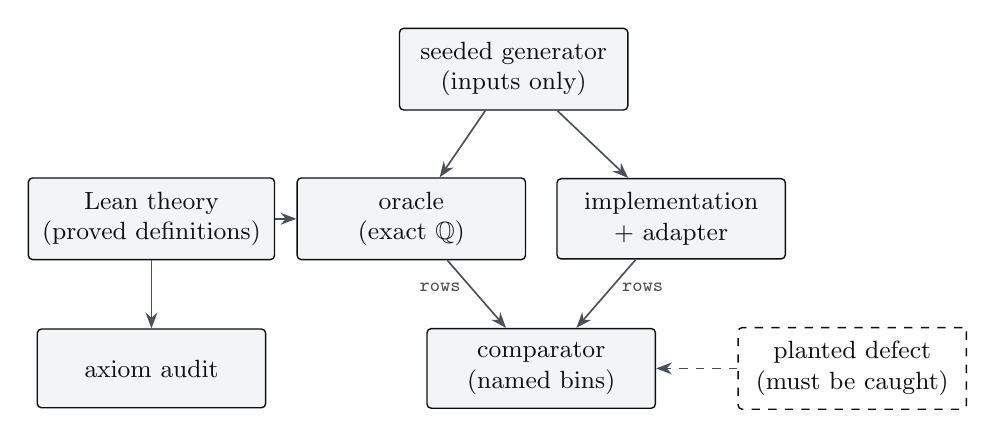
\begin{tikzpicture}[
  box/.style={draw=Ink, line width=0.5pt, fill=Surface, text=Ink, rounded corners=1.5pt,
    align=center, font=\small, inner sep=5pt, minimum height=10mm, minimum width=29mm},
  arr/.style={-{Stealth[length=2mm]}, line width=0.6pt, draw=InkMuted},
  lab/.style={font=\ttfamily\scriptsize, text=InkMuted}]
\node[box] (gen) at (4.6,1.9) {seeded generator\\(inputs only)};
\node[box] (theory) at (0,0) {Lean theory\\(proved definitions)};
\node[box] (oracle) at (3.3,0) {oracle\\(exact $\mathbb{Q}$)};
\node[box] (impl) at (6.6,0) {implementation\\+ adapter};
\node[box] (cmp) at (4.95,-1.9) {comparator\\(named bins)};
\node[box] (audit) at (0,-1.9) {axiom audit};
\node[box, dashed, fill=Background] (planted) at (8.9,-1.9) {planted defect\\(must be caught)};
\draw[arr] (gen) -- (oracle);
\draw[arr] (gen) -- (impl);
\draw[arr] (theory) -- (oracle);
\draw[arr] (theory) -- (audit);
\draw[arr] (oracle) -- node[left, lab, pos=0.4] {rows} (cmp);
\draw[arr] (impl) -- node[right, lab, pos=0.4] {rows} (cmp);
\draw[arr, dashed] (planted) -- (cmp);
\end{tikzpicture}
\caption{The measurement procedure. The generator never computes expected results;
those come only from the oracle.}
\label{fig:harness}
\end{figure}

The procedure follows \texttt{ledger-semantics} (\cref{fig:harness}). A seeded
generator writes case files containing inputs only. It favors the inputs where
implementations are known to have conventions: tied logits, words that are
themselves tokens, and merge tables with several splits of one string. A small
adapter per implementation runs the same cases and prints the oracle's row format.
The comparator places every case in exactly one named bin (agree, diverge, skipped
by either side, or missing), so nothing is dropped silently. Token rows are compared
as strings. Sampler rows require that a zero be matched by a zero and that nonzero
probabilities agree within $10^{-6}$, since llama.cpp stores logits in
\texttt{float32}. Each comparator is observed to fail: a planted defect, an adapter
that glues two tokens or one that inverts temperature, must be detected or the run
fails.

\paragraph{Tie divergences.} An implementation that keeps exactly $k$ tokens breaks
ties in its own order, which need not be the oracle's order by index. Every filter
treats tied tokens alike except for that choice, and tied tokens stay tied through
temperature and renormalization. Such an implementation must therefore agree with
the positional semantics up to a permutation of tied tokens. The harness checks
exactly this: the multiset of (logit, probability) pairs over the kept tokens must
equal that of the oracle's \texttt{q} rows. A divergence that fails this check is
reported as unexplained.

\begin{table}[t]
\centering\small
\caption{Measurements (\texttt{harness/run.sh 600}: four seeds of 600 cases each per
corpus). Lean 4.34.1, Mathlib v4.34.1, \texttt{tokenizers} 0.23.3, \texttt{tiktoken}
0.14.0, llama.cpp commit \texttt{a9d27ac} (2026-10-11).}
\label{tab:results}
\begin{tabularx}{\linewidth}{@{}>{\raggedright\arraybackslash}p{4.6cm}>{\raggedright\arraybackslash}X>{\raggedright\arraybackslash}X@{}}
\toprule
\qpth{Implementation} & \qpth{Compared against} & \qpth{Result}\\
\midrule
HF \texttt{tokenizers}, BPE, defaults & rule-rank BPE (\lean{bpe}) & 13{,}779 / 13{,}779 words identical\\
HF \texttt{tokenizers}, \lean{ignore_merges} & lookup, then rule-rank BPE & 13{,}779 / 13{,}779 identical\\
\texttt{tiktoken} & lookup, then concatenation-rank BPE & 13{,}779 / 13{,}779 identical\\
llama.cpp \lean{top_k}, \lean{top_p}, \lean{min_p}, \texttt{temp}, no ties & tie-keeping filters & 1{,}216 / 1{,}216 chains, $|\Delta p|\le5.1\times10^{-8}$\\
llama.cpp, with ties & tie-keeping, else positional & 939 + 245 / 1{,}184 chains; 0 unexplained\\
Planted defects (tokenizer, sampler) & --- & both detected\\
\bottomrule
\end{tabularx}
\end{table}

\Cref{tab:results} summarizes the results. Two findings came out of the
comparisons. First, \texttt{tiktoken} initially disagreed with the oracle's
concatenation-rank BPE on words that are themselves vocabulary tokens. The
disagreement was a convention, whole-word lookup. Following the
\texttt{ledger-semantics} rule that a divergence is either a defect in the
implementation or a convention the semantics has not yet recorded, we recorded it
as \lean{lookupFirst}, with its own theorems, after which agreement is exact.
Second, on the same random merge tables the two tokenizer libraries disagree with
each other on 439 of 13{,}779 words (3.2\%), and on 279 when Hugging Face uses
\lean{ignore_merges}. The oracle reproduces each library exactly, so every one of
these disagreements is predicted. \Cref{thm:bpeconv} states the condition under which
they cannot occur.

For sampling, llama.cpp agrees with the tie-keeping semantics on every tie-free
chain. On chains with ties, 245 of 1{,}184 diverge, and every one agrees with the
positional semantics up to a permutation of tied tokens. Some of these divergences
cascade: a tie cut by top-$k$ changes the renormalized masses that a later top-$p$
sees. A check that compared kept sets only after the fact would misclassify such
cases. Replaying the convention exactly classifies all of them.

% ===========================================================================
\section{Related work}

\paragraph{Formal methods for machine learning.} Most verification work on neural
networks proves properties of trained models, for example with SMT-based
methods~\cite{katz2017reluplex}. We verify the model-independent algorithms around
the model instead, and connect them to implementations through an oracle. The
denotational method follows Elliott~\cite{elliott2009denotational}. The use of a
proved semantics as a test oracle, the procedure of planted defects, and the
discipline of named skip bins follow \texttt{ledger-semantics}~\cite{ledgersemantics}.
Our category of finite stochastic maps is a special case of Fritz's Markov
categories~\cite{fritz2020markov}.

\paragraph{Tokenization.} Zouhar et al.\ give a formal analysis of BPE as an
optimization problem~\cite{zouhar2023bpe}. Gastaldi et al.\ treat tokenizers as
stochastic maps and study consistency of estimators~\cite{gastaldi2024foundations}.
Vieira et al.\ show how to turn token-level models into character-level
ones~\cite{vieira2024tokens}, which requires exactly the enumeration of
tokenizations we verify. Our no-compression theorem and the agreement criterion
between BPE conventions complement this work at the level of exact identities.

\paragraph{Decoding.} Top-$k$~\cite{fan2018hierarchical}, nucleus~\cite{holtzman2020curious}
and min-$p$~\cite{nguyen2025minp} sampling are usually specified by an algorithm over
sorted arrays, which leaves ties unspecified. \Cref{thm:topk} shows that this gap
cannot be closed by any symmetric rule. Speculative
sampling~\cite{leviathan2023speculative,chen2023speculative} is known to be lossless,
and its acceptance rate is the maximal-coupling bound~\cite{lindvall1992coupling}. Du et
al.\ characterize tightness measure-theoretically~\cite{du2023tight}. We give a
finite-depth statement and an explicit non-tight model.

\paragraph{Attention and inference systems.} Online softmax~\cite{milakov2018online}
underlies FlashAttention~\cite{dao2022flashattention} and its successors, and
KV caching is standard in serving systems~\cite{pope2023scaling,kwon2023vllm}. Our
contribution is the algebraic packaging, a commutative monoid with a free-monoid
homomorphism, and machine-checked proofs over arbitrary exponential characters.
Permutation equivariance of attention without positional encodings is
known~\cite{yun2020universal}.

\paragraph{Masked diffusion.} The time-independence of the optimal denoiser was
observed by Ou et al.~\cite{ou2025absorbing}, in the setting of
D3PM~\cite{austin2021d3pm}, MDLM~\cite{sahoo2024mdlm} and related
models~\cite{shi2024masked,nie2025llada}. We machine-check it, together with the
any-order chain rule and the inexactness of parallel unmasking.

% ===========================================================================
\section{Limitations}

Analysis on the reals enters only through exponential characters, and there is no
measure theory, so sampling and tightness are stated through finite quantities. The
oracle's temperature is restricted to $1/n$, which keeps softmax rational. The
theorems hold for every temperature, but the oracle cannot evaluate an irrational
softmax. Speculative decoding is proved for one drafted token. The sequence version
follows by induction and is not yet formalized. Nothing is proved about
floating-point arithmetic: implementations are compared with exact values within a
stated tolerance. A decision that lies exactly on a floating-point boundary could in
principle diverge, and none occurred in our runs. The diffusion theory covers
absorbing diffusion, not Gaussian diffusion. The chat protocol models tool calling in
its common request-and-result form, not any vendor's specification. The measurements
cover tokenizers and samplers; attention kernels, speculative decoders, chat
renderers and diffusion samplers are evaluated by the oracle but not yet compared
against implementations.

% ===========================================================================
\section{Conclusion}

The inference side of LLMs is small enough to be given a precise meaning and large
enough that its implementations disagree. A machine-checked semantics separates
what is meaning from what is convention. It proves which reorderings, cachings and
tilings are harmless, and it shows that some properties folklore expects, such as
symmetric exact top-$k$, compositional compressing tokenizers and unambiguous plain-text
templates, cannot exist. Connected to an exact oracle, the same definitions become
a test instrument. Every divergence it surfaces is either a defect in an
implementation or a convention that belongs in the semantics.

\paragraph{Availability.} The Lean development, oracle, harness, and recorded
measurement log accompany this paper.

\paragraph{Acknowledgments.} The structure of this work follows
\texttt{ledger-semantics} by John Wiegley. The formalization and harness were
developed with the assistance of an AI system (Claude, Anthropic).

% ===========================================================================
\begin{thebibliography}{99}\small

\bibitem{austin2021d3pm}
J.~Austin, D.~D. Johnson, J.~Ho, D.~Tarlow, and R.~van~den Berg.
\newblock Structured denoising diffusion models in discrete state-spaces.
\newblock In \emph{NeurIPS}, 2021.

\bibitem{chen2023speculative}
C.~Chen, S.~Borgeaud, G.~Irving, J.-B. Lespiau, L.~Sifre, and J.~Jumper.
\newblock Accelerating large language model decoding with speculative sampling.
\newblock arXiv:2302.01318, 2023.

\bibitem{dao2022flashattention}
T.~Dao, D.~Y. Fu, S.~Ermon, A.~Rudra, and C.~R{\'e}.
\newblock {FlashAttention}: Fast and memory-efficient exact attention with {IO}-awareness.
\newblock In \emph{NeurIPS}, 2022.

\bibitem{demoura2021lean4}
L.~de~Moura and S.~Ullrich.
\newblock The {Lean} 4 theorem prover and programming language.
\newblock In \emph{CADE-28}, 2021.

\bibitem{du2023tight}
L.~Du, L.~Torroba~Hennigen, T.~Pimentel, C.~Meister, J.~Eisner, and R.~Cotterell.
\newblock A measure-theoretic characterization of tight language models.
\newblock In \emph{ACL}, 2023.

\bibitem{elliott2009denotational}
C.~Elliott.
\newblock Denotational design with type class morphisms.
\newblock Technical Report 2009-01, LambdaPix, 2009.

\bibitem{fan2018hierarchical}
A.~Fan, M.~Lewis, and Y.~Dauphin.
\newblock Hierarchical neural story generation.
\newblock In \emph{ACL}, 2018.

\bibitem{fritz2020markov}
T.~Fritz.
\newblock A synthetic approach to {Markov} kernels, conditional independence and theorems on sufficient statistics.
\newblock \emph{Advances in Mathematics}, 370, 2020.

\bibitem{gastaldi2024foundations}
J.~L. Gastaldi, J.~Terilla, L.~Malagutti, B.~DuSell, T.~Vieira, and R.~Cotterell.
\newblock The foundations of tokenization: Statistical and computational concerns.
\newblock arXiv:2407.11606, 2024.

\bibitem{greshake2023injection}
K.~Greshake, S.~Abdelnabi, S.~Mishra, C.~Endres, T.~Holz, and M.~Fritz.
\newblock Not what you've signed up for: Compromising real-world {LLM}-integrated applications with indirect prompt injection.
\newblock In \emph{AISec}, 2023.

\bibitem{holtzman2020curious}
A.~Holtzman, J.~Buys, L.~Du, M.~Forbes, and Y.~Choi.
\newblock The curious case of neural text degeneration.
\newblock In \emph{ICLR}, 2020.

\bibitem{katz2017reluplex}
G.~Katz, C.~Barrett, D.~L. Dill, K.~Julian, and M.~J. Kochenderfer.
\newblock Reluplex: An efficient {SMT} solver for verifying deep neural networks.
\newblock In \emph{CAV}, 2017.

\bibitem{kwon2023vllm}
W.~Kwon, Z.~Li, S.~Zhuang, Y.~Sheng, L.~Zheng, C.~H. Yu, J.~E. Gonzalez, H.~Zhang, and I.~Stoica.
\newblock Efficient memory management for large language model serving with {PagedAttention}.
\newblock In \emph{SOSP}, 2023.

\bibitem{ledgersemantics}
J.~Wiegley.
\newblock ledger-semantics: Mathematical semantics of {Ledger}, the double-entry accounting tool.
\newblock \url{https://github.com/ledger/ledger-semantics}, 2026.

\bibitem{leviathan2023speculative}
Y.~Leviathan, M.~Kalman, and Y.~Matias.
\newblock Fast inference from transformers via speculative decoding.
\newblock In \emph{ICML}, 2023.

\bibitem{lindvall1992coupling}
T.~Lindvall.
\newblock \emph{Lectures on the Coupling Method}.
\newblock Wiley, 1992.

\bibitem{liu2023ring}
H.~Liu, M.~Zaharia, and P.~Abbeel.
\newblock Ring attention with blockwise transformers for near-infinite context.
\newblock arXiv:2310.01889, 2023.

\bibitem{mathlib2020}
The mathlib Community.
\newblock The {Lean} mathematical library.
\newblock In \emph{CPP}, 2020.

\bibitem{milakov2018online}
M.~Milakov and N.~Gimelshein.
\newblock Online normalizer calculation for softmax.
\newblock arXiv:1805.02867, 2018.

\bibitem{nguyen2025minp}
M.~N. Nguyen, A.~Baker, C.~Neo, A.~Roush, A.~Kirsch, and R.~Shwartz-Ziv.
\newblock Turning up the heat: Min-p sampling for creative and coherent {LLM} outputs.
\newblock In \emph{ICLR}, 2025.

\bibitem{nie2025llada}
S.~Nie, F.~Zhu, Z.~You, X.~Zhang, J.~Ou, J.~Hu, J.~Zhou, Y.~Lin, J.-R. Wen, and C.~Li.
\newblock Large language diffusion models.
\newblock arXiv:2502.09992, 2025.

\bibitem{ou2025absorbing}
J.~Ou, S.~Nie, K.~Xue, F.~Zhu, J.~Sun, Z.~Li, and C.~Li.
\newblock Your absorbing discrete diffusion secretly models the conditional distributions of clean data.
\newblock In \emph{ICLR}, 2025.

\bibitem{pope2023scaling}
R.~Pope, S.~Douglas, A.~Chowdhery, J.~Devlin, J.~Bradbury, J.~Heek, K.~Xiao, S.~Agrawal, and J.~Dean.
\newblock Efficiently scaling transformer inference.
\newblock In \emph{MLSys}, 2023.

\bibitem{rabe2021selfattention}
M.~N. Rabe and C.~Staats.
\newblock Self-attention does not need {$O(n^2)$} memory.
\newblock arXiv:2112.05682, 2021.

\bibitem{radford2019gpt2}
A.~Radford, J.~Wu, R.~Child, D.~Luan, D.~Amodei, and I.~Sutskever.
\newblock Language models are unsupervised multitask learners.
\newblock OpenAI technical report, 2019.

\bibitem{sahoo2024mdlm}
S.~S. Sahoo, M.~Arriola, Y.~Schiff, A.~Gokaslan, E.~Marroquin, J.~T. Chiu, A.~Rush, and V.~Kuleshov.
\newblock Simple and effective masked diffusion language models.
\newblock In \emph{NeurIPS}, 2024.

\bibitem{sennrich2016bpe}
R.~Sennrich, B.~Haddow, and A.~Birch.
\newblock Neural machine translation of rare words with subword units.
\newblock In \emph{ACL}, 2016.

\bibitem{shi2024masked}
J.~Shi, K.~Han, Z.~Wang, A.~Doucet, and M.~K. Titsias.
\newblock Simplified and generalized masked diffusion for discrete data.
\newblock In \emph{NeurIPS}, 2024.

\bibitem{vieira2024tokens}
T.~Vieira, B.~LeBrun, M.~Giulianelli, J.~L. Gastaldi, B.~DuSell, J.~Terilla, T.~J. O'Donnell, and R.~Cotterell.
\newblock From language models over tokens to language models over characters.
\newblock arXiv:2412.03719, 2024.

\bibitem{wolf2020transformers}
T.~Wolf et~al.
\newblock Transformers: State-of-the-art natural language processing.
\newblock In \emph{EMNLP: System Demonstrations}, 2020.

\bibitem{xiao2024sinks}
G.~Xiao, Y.~Tian, B.~Chen, S.~Han, and M.~Lewis.
\newblock Efficient streaming language models with attention sinks.
\newblock In \emph{ICLR}, 2024.

\bibitem{yun2020universal}
C.~Yun, S.~Bhojanapalli, A.~S. Rawat, S.~J. Reddi, and S.~Kumar.
\newblock Are transformers universal approximators of sequence-to-sequence functions?
\newblock In \emph{ICLR}, 2020.

\bibitem{zouhar2023bpe}
V.~Zouhar, C.~Meister, J.~L. Gastaldi, L.~Du, T.~Vieira, M.~Sachan, and R.~Cotterell.
\newblock A formal perspective on byte-pair encoding.
\newblock In \emph{Findings of ACL}, 2023.

\end{thebibliography}

\end{document}
"

\usepackage[a4paper,textwidth=15.4cm,textheight=23.6cm,top=3.0cm,headsep=0.9cm,footskip=1.2cm]{geometry}
\usepackage{amsmath,amssymb,amsthm,mathtools}
\usepackage{fontspec}
\usepackage{booktabs,tabularx,array}
\usepackage[protrusion=true,expansion=false]{microtype}
\usepackage[table]{xcolor}
\usepackage{graphicx}
\usepackage{fvextra}
\usepackage{enumitem}
\usepackage{caption}
\usepackage{titlesec}
\usepackage{fancyhdr}
\usepackage[most]{tcolorbox}
\usepackage{tikz}
\usetikzlibrary{arrows.meta}
\usepackage{hyperref}
\usepackage[nameinlink,capitalise]{cleveref}

% ---------------------------------------------------------------------------
%  Colour tokens
% ---------------------------------------------------------------------------
% Neutral foundation. Ink and Background invert between the two editions.
\ifqptdark
  \definecolor{Background}{HTML}{0B0C0E}
  \definecolor{Surface}{HTML}{16181B}
  \definecolor{Border}{HTML}{2B2E33}
  \definecolor{Ink}{HTML}{EDEEF0}
  \definecolor{InkMuted}{HTML}{A9AEB6}
  \definecolor{InkFaint}{HTML}{5A5F67}   % decoration only, never meaningful text
\else
  \definecolor{Background}{HTML}{FFFFFF}
  \definecolor{Surface}{HTML}{F3F4F5}
  \definecolor{Border}{HTML}{DADDE1}
  \definecolor{Ink}{HTML}{0E0F11}
  \definecolor{InkMuted}{HTML}{4B4F57}
  \definecolor{InkFaint}{HTML}{A3A7AE}   % decoration only, never meaningful text
\fi
% Paradigm colours: fixed in both editions, semantic only.
\definecolor{Quantum}{HTML}{5BAD1E}
\definecolor{Photonic}{HTML}{F0AB00}
\definecolor{Thermodynamic}{HTML}{E8690A}
\definecolor{Ternary}{HTML}{8A8A8A}
\definecolor{Bio}{HTML}{1AAB7C}

\ifqptdark\pagecolor{Background}\fi

% ---------------------------------------------------------------------------
%  Typography
% ---------------------------------------------------------------------------
\setmainfont{Inter}[
  Path=fonts/, Extension=.otf, Scale=0.94,
  UprightFont=*-Regular, ItalicFont=*-Italic,
  BoldFont=*-SemiBold, BoldItalicFont=*-SemiBoldItalic]
\setmonofont{IBMPlexMono}[
  Path=fonts/, Extension=.ttf, Scale=MatchLowercase,
  UprightFont=*-Regular, ItalicFont=*-Italic, BoldFont=*-SemiBold]
\newfontfamily\qptdisplay{SpaceGrotesk}[
  Path=fonts/, Extension=.otf, UprightFont=*-Medium, BoldFont=*-Bold]
\newfontfamily\qptdisplaylight{SpaceGrotesk}[
  Path=fonts/, Extension=.otf, UprightFont=*-Regular]
\newfontfamily\qptlabelfont{IBMPlexMono}[
  Path=fonts/, Extension=.ttf, Scale=MatchLowercase, UprightFont=*-Medium,
  LetterSpace=6]
\setsansfont{Inter}[
  Path=fonts/, Extension=.otf, Scale=0.94,
  UprightFont=*-Regular, ItalicFont=*-Italic,
  BoldFont=*-SemiBold, BoldItalicFont=*-SemiBoldItalic]
\linespread{1.16}
\setlength{\emergencystretch}{2.5em}
\AtBeginDocument{\raggedright\setlength{\parindent}{0pt}}
\setlength{\parindent}{0pt}
\setlength{\parskip}{0.55em}

% A label: IBM Plex Mono, upper case, tracked.
\newcommand{\qptlabel}[1]{{\qptlabelfont\footnotesize\MakeUppercase{#1}}}
% Technical names (Lean declarations, files) in IBM Plex Mono.
\newcommand{\lean}[1]{\texttt{\detokenize{#1}}}
\newcommand{\leanref}[1]{\par\smallskip\noindent
  {\ttfamily\footnotesize\upshape\raggedright\color{InkMuted}LEAN\enspace #1\par}}

% Ink is the normal colour everywhere, including floats, heads and footnotes.
\makeatletter
\AtBeginDocument{\color{Ink}\global\let\default@color\current@color}
\makeatother

% ---------------------------------------------------------------------------
%  Mathematical notation
% ---------------------------------------------------------------------------
\newcommand{\K}{\Bbbk}
\newcommand{\Dist}{\mathrm{Dist}}
\newcommand{\restr}[2]{#1|_{#2}}
\newcommand{\topk}{\mathrm{TopK}}
\newcommand{\topp}{\mathrm{TopP}}
\newcommand{\minp}{\mathrm{MinP}}
\newcommand{\sharpen}{\mathrm{sharpen}}
\newcommand{\abv}{\mathrm{above}}
\newcommand{\tv}{\mathrm{tv}}
\newcommand{\dec}{\mathrm{dec}}
\newcommand{\enc}{\mathrm{enc}}
\newcommand{\softmax}{\mathrm{softmax}}
\newcommand{\attend}{\mathrm{attend}}
\newcommand{\Iv}[1]{[\![#1]\!]}
\newcommand{\Mask}{\bot}

% ---------------------------------------------------------------------------
%  Headings: section numbers as labels, titles in Space Grotesk
% ---------------------------------------------------------------------------
\makeatletter
\newcommand{\qptsecnum}[1]{{\qptlabelfont\small\color{InkMuted}\two@digits{#1}}}
\makeatother
\titleformat{\section}
  {\qptdisplay\fontsize{14.5}{18}\selectfont\color{Ink}}
  {\qptsecnum{\value{section}}}{0.9em}{}
\titleformat{name=\section,numberless}
  {\qptdisplay\fontsize{14.5}{18}\selectfont\color{Ink}}{}{0pt}{}
\titlespacing*{\section}{0pt}{1.9em}{0.7em}
\titleformat{\paragraph}[runin]
  {\qptdisplay\normalsize\color{Ink}}{}{0pt}{}
\titlespacing*{\paragraph}{0pt}{0.9em}{0.6em}

% ---------------------------------------------------------------------------
%  Statements
% ---------------------------------------------------------------------------
\newtheoremstyle{qpt}
  {0.9em}{0.9em}
  {\normalfont}{}
  {\qptlabelfont\footnotesize}{}
  {\newline}
  {\MakeUppercase{\thmname{#1}\thmnumber{~#2}}%
   \thmnote{\enspace{\qptdisplay\normalsize\color{Ink}#3}}}
\theoremstyle{qpt}
\newtheorem{theorem}{Theorem}
\newtheorem{proposition}[theorem]{Proposition}
\newtheorem{corollary}[theorem]{Corollary}
\newtheorem{lemma}[theorem]{Lemma}
\newtheorem{definition}[theorem]{Definition}
\newtheorem{remark}[theorem]{Remark}

% Proofs: a tracked label and a neutral end mark.
\makeatletter
\renewcommand{\qedsymbol}{{\color{InkMuted}\rule{0.5em}{0.5em}}}
\renewenvironment{proof}[1][Proof]{\par\pushQED{\qed}\normalfont\topsep0.5em\relax
  \trivlist\item[\hskip\labelsep\qptlabel{#1}\hspace{0.6em}]\ignorespaces}
  {\popQED\endtrivlist\@endpefalse}
\makeatother

% ---------------------------------------------------------------------------
%  Code: IBM Plex Mono on a neutral surface, with a hairline on the left
% ---------------------------------------------------------------------------
\tcbset{colupper=Ink, collower=Ink}
\tcbset{qptcode/.style={enhanced, colback=Surface, colframe=Surface,
  boxrule=0pt, arc=0pt, left=9pt, right=8pt, top=5pt, bottom=5pt,
  borderline west={1.2pt}{0pt}{InkFaint}, before skip=0.7em, after skip=0.7em}}
\newenvironment{leancode}
  {\VerbatimEnvironment\begin{tcolorbox}[qptcode]%
   \begin{Verbatim}[fontsize=\small,commandchars=\\\{\},
     codes={\catcode`\$=3\catcode`\^=7},formatcom=\color{Ink}]}
  {\end{Verbatim}\end{tcolorbox}}
\newenvironment{casecode}
  {\VerbatimEnvironment\begin{tcolorbox}[qptcode,before skip=0pt,after skip=0pt]%
   \begin{Verbatim}[fontsize=\footnotesize,formatcom=\color{Ink}]}
  {\end{Verbatim}\end{tcolorbox}}

% ---------------------------------------------------------------------------
%  Floats, tables, captions
% ---------------------------------------------------------------------------
\DeclareCaptionLabelFormat{qpt}{\qptlabel{#1~#2}}
\DeclareCaptionLabelSeparator{qptsep}{\quad}
\captionsetup{labelformat=qpt, labelsep=qptsep, font={small,color=Ink},
  justification=raggedright, singlelinecheck=false, skip=6pt}
\newcommand{\qpth}[1]{\qptlabel{#1}}
\arrayrulecolor{Ink}
\setlength{\heavyrulewidth}{0.7pt}
\setlength{\lightrulewidth}{0.35pt}
\renewcommand{\arraystretch}{1.22}

% ---------------------------------------------------------------------------
%  Running heads
% ---------------------------------------------------------------------------
\pagestyle{fancy}
\fancyhf{}
\fancyhead[L]{{\color{Ink}\qptlabel{Machine-checked semantics of LLM inference}}}
\fancyhead[R]{{\color{Ink}\qptlabel{D. Arango Sohm}}}
\fancyfoot[R]{{\ttfamily\small\color{InkMuted}\thepage}}
\renewcommand{\headrule}{{\color{Border}\hrule height 0.4pt}\vspace{-0.4pt}}
\renewcommand{\headrulewidth}{0.4pt}
\fancypagestyle{qptfirst}{\fancyhf{}%
  \fancyfoot[R]{{\ttfamily\small\color{InkMuted}\thepage}}%
  \renewcommand{\headrulewidth}{0pt}\renewcommand{\headrule}{}}

% ---------------------------------------------------------------------------
%  Links and references: neutral, never accent-coloured text
% ---------------------------------------------------------------------------
\hypersetup{colorlinks=true, linkcolor=Ink, citecolor=Ink, urlcolor=Ink,
  pdftitle={A Machine-Checked Semantics of LLM Inference},
  pdfauthor={Daniel Arango Sohm},
  pdfsubject={Formal semantics of large language model inference in Lean 4},
  pdfkeywords={Lean 4, Mathlib, formal verification, LLM inference, sampling,
    tokenization, attention, speculative decoding, diffusion language models}}
\makeatletter
\renewcommand{\@biblabel}[1]{{\ttfamily\color{InkMuted}[#1]}}
\renewcommand{\@cite}[2]{{\ttfamily[#1\if@tempswa, #2\fi]}}
\makeatother
\renewcommand{\refname}{References}

\setlist{itemsep=2pt, topsep=4pt}
\setlist[itemize]{label={\color{InkMuted}\textbullet}}

\begin{document}
\thispagestyle{qptfirst}

% ----------------------------------------------------------------- masthead
\noindent
\begin{minipage}[c]{0.5\linewidth}
  \includegraphics[height=1.9cm]{qpt-logo.png}
\end{minipage}%
\begin{minipage}[c]{0.5\linewidth}\raggedleft
  \qptlabel{Preprint}\\[2pt]
  \qptlabel{October 2026}
\end{minipage}

\vspace{1.6em}
{\color{Border}\rule{\linewidth}{0.4pt}}
\vspace{1.1em}

{\qptdisplay\fontsize{25}{29.5}\selectfont\color{Ink}
A Machine-Checked Semantics\\ of LLM Inference\par}
\vspace{0.55em}
{\qptdisplaylight\fontsize{13}{17}\selectfont\color{InkMuted}
Sampling, Attention, Tokenization, Chat, Decoding,\\ and Diffusion in Lean~4\par}

\vspace{1.5em}
{\large\bfseries Daniel Arango Sohm}\par
\vspace{0.15em}
{\color{InkMuted}Universidad EAFIT, Medellín, Colombia\\
Former member of the QPT team}\par

\vspace{1.4em}
% ----------------------------------------------------------------- abstract
\begin{tcolorbox}[enhanced, colback=Surface, colframe=Surface, colupper=Ink, boxrule=0pt,
  arc=0pt, left=12pt, right=12pt, top=9pt, bottom=10pt]
\qptlabel{Abstract}\par\vspace{0.35em}
{\small
The inference side of a large language model is a stack of small algorithms:
tokenizers, attention kernels, key--value caches, sampling filters, speculative
decoders, chat templates, and diffusion samplers. Each has several independent
implementations, and those implementations are usually tested against one another
rather than against a definition. We give these components a single mathematical
semantics, formalized in Lean~4 against Mathlib. The development comprises about
4{,}600 lines and 270 named theorems, and every declaration depends only on Lean's
three standard axioms. It proves the exact algebra of sampling filters, the
losslessness and optimality of speculative sampling, and the correctness of
key--value caching and of FlashAttention-style online softmax as a commutative
monoid. It proves that byte-pair encoding is lossless under every merge priority,
together with a decidable criterion for when the Hugging Face and \texttt{tiktoken}
conventions agree, a protocol checker for tool calls, and the time-independence of
the masked-diffusion denoiser. It also proves six negative results. No sampling
rule that treats tokens symmetrically can always keep exactly $k$ tokens. No
tokenizer that compresses can respect concatenation. Every chat template that writes
its role markers in the content alphabet is ambiguous. No transformer without
positional information can copy a fixed position. An autoregressive model need not
define a distribution over strings. Parallel unmasking in diffusion is inexact.
From the same definitions we build an executable oracle that evaluates test cases in
exact rational arithmetic, and a harness that measures implementations against it.
On 2{,}400 random merge tables, Hugging Face \texttt{tokenizers} and
\texttt{tiktoken} each agree with the oracle on all 13{,}779 test words, while
disagreeing with each other on 3.2\% of them. On 2{,}400 random sampler chains,
every divergence of llama.cpp from the tie-keeping semantics is accounted for
exactly by the positional semantics that the impossibility theorem forces.
\par}
\end{tcolorbox}

\vspace{0.3em}
\noindent\qptlabel{Keywords}\enspace{\small Lean~4 · Mathlib · formal verification ·
LLM inference · sampling · tokenization · attention · speculative decoding ·
diffusion language models}

\vspace{0.4em}
{\color{Border}\rule{\linewidth}{0.4pt}}

% ===========================================================================
\section{Introduction}

A deployed language model is a function from parameters and a context to a
distribution over tokens. Turning that distribution into text requires more
machinery. A tokenizer maps strings to token sequences. Attention kernels compute
the model's reads over a cached context. A chain of sampling filters reshapes the
next-token distribution. A speculative decoder may verify drafted tokens, a chat
template linearizes a conversation, and a diffusion sampler may unmask several
positions at once. Each of these components exists in many implementations, such as
Hugging Face \texttt{transformers} and \texttt{tokenizers}~\cite{wolf2020transformers},
\texttt{tiktoken}, vLLM~\cite{kwon2023vllm}, and llama.cpp. Their tests mostly
compare one implementation with another, or with remembered behavior.

This paper follows a different discipline, \emph{denotational design}~\cite{elliott2009denotational}.
One first says precisely what a thing means, then requires every operation to
preserve that meaning, and lets the implementation be whatever the equations force
it to be. The approach is that of \texttt{ledger-semantics}~\cite{ledgersemantics},
which formalizes double-entry accounting in Lean and uses the result as a test oracle
for the C++ Ledger program. We apply it to LLM inference. A sampling filter means
conditioning a distribution on a set. A KV-cached decoder means causal attention over
the whole prefix. A FlashAttention kernel means a softmax-weighted average. A chat
template means an injective encoding of a transcript. The theorems state when an
implementation preserves that meaning, and several of them state that no
implementation can.

\paragraph{Contributions.}
\begin{itemize}[leftmargin=*,itemsep=2pt]
\item A Lean~4 formalization against Mathlib~\cite{mathlib2020,demoura2021lean4}
  of sampling, speculative decoding, softmax and attention, tokenization, chat
  transcripts, autoregressive decoding, and masked diffusion
  (\cref{sec:foundations,sec:sampling,sec:spec,sec:attention,sec:tokenization,sec:chat,sec:decoding,sec:diffusion}).
  All definitions are stated over an arbitrary linearly ordered field, so one proof
  covers the real numbers of the literature and the exact rationals of the oracle.
\item Positive results in a common framework. They include the algebra of
  sampling filters, the optimality of speculative sampling, an online-softmax
  commutative monoid, a generic correctness theorem for BPE with a decidable
  agreement criterion between the two conventions in use, a protocol checker for
  tool calls, and the any-order chain rule for masked diffusion.
\item Six negative results that explain design constraints visible across
  implementations (\cref{sec:negative}).
\item An executable oracle that evaluates case files under the proved
  definitions in exact arithmetic, and a measurement of Hugging Face
  \texttt{tokenizers}, \texttt{tiktoken}, and llama.cpp against it (\cref{sec:oracle,sec:measure}).
\end{itemize}

Several of the positive results are known: losslessness of speculative
sampling~\cite{leviathan2023speculative,chen2023speculative}, correctness of online
softmax~\cite{milakov2018online,dao2022flashattention}, time-independence of the
absorbing-diffusion posterior~\cite{ou2025absorbing}, and the role of permutation
equivariance~\cite{yun2020universal}. Our contribution for these is a machine-checked
statement in one framework, connected to an oracle. To our knowledge the
following are not stated elsewhere in the form given here: the impossibility of
symmetric exact top-$k$ and nucleus selection, the no-compression theorem for
homomorphic tokenizers, the ambiguity of every in-band chat template, and the
decidable agreement criterion between merge-rule and concatenation-rank BPE.

% ===========================================================================
\section{Method and trust base}\label{sec:method}

The development is a Lean~4 library (Lean 4.34.1, Mathlib v4.34.1) of eleven
theory modules and two executable modules (\cref{tab:modules}). It is built with
warnings promoted to errors, so an unproved theorem (\lean{sorry}) fails the build.
A separate audit program walks every declaration in the library, 853 in all, and
fails unless each depends only on propositional extensionality, the axiom of choice,
and quotient soundness. The audit has been observed to fail: a planted proof by
\lean{native_decide}, which introduces an auxiliary axiom trusting compiled code, is
rejected. The warnings-as-errors build alone does not catch it. Concrete
counterexamples are therefore proved by \lean{decide}, whose certificate the kernel
checks by evaluation.

\begin{table}[t]
\centering\small
\caption{Modules of the development. Lines and named theorems and lemmas per module.}
\label{tab:modules}
\begin{tabularx}{\linewidth}{@{}l>{\raggedright\arraybackslash}X>{\ttfamily}r>{\ttfamily}r@{}}
\toprule
\qpth{Module} & \qpth{Content} & \qpth{Lines} & \qpth{Thms} \\
\midrule
\lean{Dist} & finite distributions, conditioning, total variation, $\mathsf{FinStoch}$ & 383 & 34\\
\lean{Sampling} & top-$k$, top-$p$, min-$p$, temperature, ties, inverse CDF & 732 & 46\\
\lean{Counterexamples} & kernel-checked failures of sampler laws & 52 & 4\\
\lean{Speculative} & speculative sampling, couplings & 194 & 17\\
\lean{Softmax} & exponential characters, masking, temperature & 220 & 23\\
\lean{Attention} & equivariance, causality, KV cache, online softmax & 573 & 38\\
\lean{Real} & $\exp$ as a character; textbook restatements & 51 & 4\\
\lean{Tokenization} & free-monoid decoding, BPE conventions, enumeration & 860 & 49\\
\lean{Chat} & tool-call protocol, rendering & 440 & 21\\
\lean{Decoding} & mass conservation, tightness, greedy decoding & 245 & 15\\
\lean{Diffusion} & masked diffusion, posterior, chain rule & 379 & 18\\
\lean{Oracle}, \lean{Driver} & case parsing and exact evaluation & 465 & 1\\
\midrule
Total & & 4{,}594 & 270\\
\bottomrule
\end{tabularx}
\end{table}

\paragraph{Numbers.} Every probability lives in an arbitrary field $\K$ with a
compatible linear order (\lean{[Field K] [LinearOrder K] [IsStrictOrderedRing K]}).
The oracle instantiates $\K=\mathbb{Q}$, so its arithmetic is exact. The analytic
statements instantiate $\K=\mathbb{R}$. No measure theory is used. Sampling is made
precise through interval statements (\cref{thm:invcdf}), and tightness through
masses at finite depth (\cref{sec:decoding}).

% ===========================================================================
\section{Foundations}\label{sec:foundations}

\begin{definition}[Finite distribution]
For a finite type $\alpha$, $\Dist_\K(\alpha)$ is the type of functions
$p:\alpha\to\K$ with $p(a)\ge 0$ for all $a$ and $\sum_a p(a)=1$.
\leanref{\lean{Dist}}
\end{definition}

\begin{leancode}
structure Dist ($\K$ : Type u) [Field $\K$] [LinearOrder $\K$] [IsStrictOrderedRing $\K$]
    ($\alpha$ : Type v) [Fintype $\alpha$] where
  prob : $\alpha$ $\to$ $\K$
  nonneg : $\forall$ a, 0 $\le$ prob a
  sum_eq_one : $\sum$ a, prob a = 1
\end{leancode}

The single operation through which masks, filters and grammar constraints act is
conditioning. For $S\subseteq\alpha$ with $p(S)>0$, write
$\restr{p}{S}(a)=\Iv{a\in S}\,p(a)/p(S)$ (\lean{Dist.restrict}).

\begin{lemma}[Conditioning]\label{lem:restrict}
$\restr{(\restr{p}{S})}{T}=\restr{p}{S\cap T}$ whenever the masses involved are
positive. Moreover $\restr{p}{S}=\restr{p}{S'}$ whenever $S$ and $S'$ contain the same
outcomes of positive probability.
\leanref{\lean{restrict_restrict}, \lean{restrict_congr}}
\end{lemma}

The finite distribution monad (point masses and \lean{bind}) satisfies the monad
laws. Finite types and stochastic maps $\alpha\to\Dist_\K(\beta)$ form a category
$\mathsf{FinStoch}_\K$, given as an instance of Mathlib's \lean{Category} whose
composition is Kleisli composition (\lean{FinStoch.category}). Total variation is
$\tv(p,q)=\sum_a\max(0,p(a)-q(a))$. We prove
$\tv(p,q)=\tfrac12\sum_a|p(a)-q(a)|$, $\sum_a\min(p(a),q(a))=1-\tv(p,q)$, and
$\tv(p,q)=0\iff p=q$.

% ===========================================================================
\section{Sampling}\label{sec:sampling}

Let $V$ be a finite vocabulary and $p:V\to\K$. Write
$\abv_p(v)=\{u: p(v)<p(u)\}$ for the tokens strictly preferred to $v$. The three
standard filters keep the sets
\begin{gather*}
\topk_k(p)=\{v: |\abv_p(v)|<k\},\qquad
\minp_m(p)=\{v:\forall u,\; m\,p(u)\le p(v)\},\\
\topp_P(p)=\Bigl\{v: \textstyle\sum_{u\in\abv_p(v)}p(u)<P\Bigr\},
\end{gather*}
and the filtered distribution is the conditioning $\restr{p}{S}$ on the kept set
$S$. For distinct probabilities, $\topp_P$ is the usual rule ``sort in descending
order and keep the shortest prefix whose mass reaches $P$''. With ties, all three
keep every tied token. Temperature $1/n$ is
$\sharpen_n(p)(v)=p(v)^n/\sum_u p(u)^n$, which stays inside $\mathbb{Q}$. In
\cref{sec:attention} we show that it equals $\softmax(n\cdot z)$ when
$p=\softmax(z)$. Every kept set contains a most probable token, provided $k\ge1$,
$P>0$ and $m\le1$, so no filter can produce an empty distribution.

\begin{theorem}[Sampler algebra]\label{thm:algebra}
For $k,k'\ge1$, $m,m'\le1$ and $n\ge1$, and writing filters in the order they are
applied,
\begin{enumerate}[label=(\roman*),itemsep=1pt]
\item top-$k$ then top-$k'$ equals top-$\min(k,k')$;
\item min-$m$ then min-$m'$ equals min-$\max(m,m')$; in particular both filters are idempotent;
\item top-$k$ and min-$m$ commute;
\item top-$k$ and temperature $1/n$ commute.
\end{enumerate}
\leanref{\lean{topK_topK}, \lean{minP_minP}, \lean{topK_minP_comm}, \lean{topK_sharpen_comm}}
\end{theorem}

\begin{proof}[Proof sketch]
All three kept sets are \emph{upward closed}: if $v$ is kept and $p(v)<p(u)$, then
$u$ is kept. Conditioning on an upward-closed set $S$ leaves $\abv(v)$ unchanged for
$v\in S$ (\lean{above_restrict}), and min-$p$ is insensitive to conditioning on a set
that contains a maximizer (\lean{minP_restrict_iff}). Each identity then reduces,
through \cref{lem:restrict}, to an equality of kept sets. For (iv), $x\mapsto x^n$
is strictly increasing on $[0,\infty)$, and top-$k$ depends only on the order of the
scores (\lean{topKSet_congr}).
\end{proof}

The laws one might expect beyond \cref{thm:algebra} are false. With
$p_0=(\tfrac12,\tfrac3{10},\tfrac15)$, the kernel evaluates the following
(\lean{Counterexamples}).

\begin{proposition}[Failed laws]\label{prop:counter}
\leavevmode\vspace{-0.5\baselineskip}
\begin{enumerate}[label=(\roman*),itemsep=1pt]
\item Top-$p$ is not idempotent: one pass of $\topp_{3/5}$ gives token~1 the probability $\tfrac38$, and a second pass gives it~$0$.
\item Top-$p$ does not commute with top-$k$: top-$p$ then top-2 leaves token~1 at $\tfrac38$, while top-2 then top-$p$ removes it.
\item Top-$p$ does not commute with temperature $\tfrac12$: token~1 ends at $\tfrac9{34}$ in one order and at $0$ in the other.
\item Min-$p$ ($m=\tfrac12$) does not commute with temperature $\tfrac12$, with the same numbers.
\end{enumerate}
\end{proposition}

A sampler chain may therefore reorder top-$k$, min-$p$ and temperature only as
\cref{thm:algebra} allows, and may not move top-$p$ at all.

\paragraph{Ties.} Implementations differ on ties, and the difference is forced.
Call a selection rule $\mathrm{sel}:(V\to\K)\to\mathcal{P}(V)$ \emph{equivariant} if
$\mathrm{sel}(p\circ\sigma^{-1})=\sigma[\mathrm{sel}(p)]$ for every permutation
$\sigma$ of $V$, that is, if relabeling the tokens relabels the output.

\begin{theorem}[No symmetric exact top-$k$]\label{thm:topk}
Let $0<k<|V|$. No equivariant selection rule satisfies $|\mathrm{sel}(p)|=k$ for
every distribution $p$.
\leanref{\lean{no_equivariant_exact_topK}}
\end{theorem}
\begin{proof}
On the uniform distribution $u$ we have $u\circ\sigma^{-1}=u$ for every $\sigma$, so
$\mathrm{sel}(u)$ is invariant under all permutations. If it contains some $v$, then
for any $w$ the transposition $(v\,w)$ maps $v$ to $w$, so it contains $w$ too.
Hence $\mathrm{sel}(u)$ is either empty or all of $V$, and neither has $k$ elements.
\end{proof}

\begin{leancode}
theorem no_equivariant_exact_topK [DecidableEq V] \char123{}k : $\mathbb{N}$\char125{}
    (hk0 : 0 < k) (hkn : k < Fintype.card V)
    (sel : (V $\to$ $\K$) $\to$ Finset V) (hsel : Equivariant sel) :
    $\neg$ $\forall$ d : Dist $\K$ V, (sel d.prob).card = k
\end{leancode}

\begin{theorem}[No symmetric smallest nucleus]
Let $V$ be nonempty and $0<P\le1-1/|V|$. No equivariant rule returns, for every
distribution, a set of minimum cardinality among those of mass at least~$P$.
\leanref{\lean{no_equivariant_exact_nucleus}}
\end{theorem}

The tie-keeping filters are equivariant (\lean{topKSet_equivariant}). The other
option is to break ties by position. Define $u\prec_p v$ if $p(u)>p(v)$, or if
$p(u)=p(v)$ and $u<v$, and let the positional filters count predecessors under
$\prec_p$ instead of $\abv_p$ (\lean{Dist.topKPos}, \lean{Dist.topPPos}).

\begin{theorem}[Positional tie-breaking]
Positional top-$k$ keeps exactly $\min(k,|V|)$ tokens. If $p$ is injective, the
positional and tie-keeping filters coincide. For $0<k<|V|$, positional top-$k$ is
not equivariant.
\leanref{\lean{card_topKPosSet}, \lean{topKPosSet_eq_of_injective}, \lean{topPPosSet_eq_of_injective}, \lean{topKPosSet_not_equivariant}}
\end{theorem}

An implementation must therefore choose between keeping exactly $k$ tokens and
treating tokens symmetrically. Hugging Face \texttt{transformers} (read from the
source of version 5.19.0) keeps ties in top-$k$, since it removes only scores
strictly below the $k$-th largest, but breaks them by sort position in top-$p$.
llama.cpp breaks ties by position in both, as measured in \cref{sec:measure}.

\begin{theorem}[Inverse-CDF sampling]\label{thm:invcdf}
Let $F(i)=\sum_{j<i}p(j)$ on $V=\{0,\dots,n-1\}$ and let $\iota(u)$ be the least $i$
with $u<F(i+1)$. For $0\le u<1$, $\iota(u)=i\iff F(i)\le u<F(i+1)$, and
$F(i+1)-F(i)=p(i)$. A uniform $u$ therefore selects $i$ with probability $p(i)$.
\leanref{\lean{invCdf_eq_iff}, \lean{cdf_interval_length}}
\end{theorem}

% ===========================================================================
\section{Speculative decoding}\label{sec:spec}

A draft model proposes $x\sim q$. The target, with distribution $p$, accepts with
probability $a(x)=\min(1,p(x)/q(x))$, and on rejection a token is drawn from the
residual $r=(p-q)^+/\tv(p,q)$~\cite{leviathan2023speculative,chen2023speculative}.
We define the joint law of (draft, emitted token) exactly as the algorithm runs,
\[
\pi(x,y)=q(x)\bigl(a(x)\,\Iv{y=x}+(1-a(x))\,r(y)\bigr).
\]

\begin{theorem}[Speculative sampling]
\leavevmode\vspace{-0.5\baselineskip}
\begin{enumerate}[label=(\roman*),itemsep=1pt]
\item The draft has law $q$: $\sum_y\pi(x,y)=q(x)$.
\item \emph{Losslessness}: the emitted token has law $p$: $\sum_x\pi(x,y)=p(y)$.
\item The acceptance probability is $\sum_x q(x)a(x)=1-\tv(p,q)$, and the emitted token equals the draft with the same probability.
\item \emph{Optimality}: every coupling $\gamma$ of $q$ and $p$ has $\sum_x\gamma(x,x)\le1-\tv(p,q)$.
\end{enumerate}
\leanref{\lean{specJoint_fst}, \lean{specJoint_snd}, \lean{accept_rate}, \lean{specJoint_diag}, \lean{coupling_le}, \lean{spec_optimal}}
\end{theorem}
\begin{proof}[Proof sketch]
Since $q(x)a(x)=\min(p(x),q(x))$, the total rejection probability is $\tv(p,q)$,
and a rejected draft is never re-emitted, because $r(x)=0$ whenever $q(x)>p(x)$. For (iv),
$\gamma(x,x)\le\min(q(x),p(x))$ by the marginal constraints. This is the classical
coupling inequality~\cite{lindvall1992coupling}.
\end{proof}

Because any lossless rule for verifying one drafted token is a coupling, (iv) shows
that speculative sampling has the highest acceptance rate any such rule can achieve.

% ===========================================================================
\section{Softmax and attention}\label{sec:attention}

\begin{definition}[Exponential character]
An \emph{exponential character} from an ordered additive group $G$ of scores into
$\K$ is a strictly increasing map $E:G\to\K$ with $E(a)>0$ and $E(a+b)=E(a)E(b)$.
For $z:\iota\to G$, $\softmax_E(z)_i=E(z_i)/\sum_jE(z_j)$.
\leanref{\lean{ExpChar}}
\end{definition}

$\exp:\mathbb{R}\to\mathbb{R}$ is a character (\lean{ExpChar.real}). So is
$z\mapsto2^z:\mathbb{Z}\to\mathbb{Q}$ (\lean{ExpChar.base2}), which the oracle uses
to evaluate softmax with no rounding. Every result in this section holds for every
character, and so for both.

\begin{theorem}[Softmax]\label{thm:softmax}
\leavevmode\vspace{-0.5\baselineskip}
\begin{enumerate}[label=(\roman*),itemsep=1pt]
\item $\softmax_E(z+c)=\softmax_E(z)$; this licenses subtracting the maximum logit.
\item $\softmax_E(z)_i<\softmax_E(z)_j\iff z_i<z_j$.
\item \emph{Masking is conditioning}: setting logits outside $S$ to $-\infty$ and taking softmax gives $\restr{\softmax_E(z)}{S}$.
\item For $G$ a field and $T>0$, $\topk_k(\softmax_E(z/T))=\topk_k(z)$.
\item $\softmax_E(n\cdot z)=\sharpen_n(\softmax_E(z))$.
\end{enumerate}
\leanref{\lean{softmax_add_const}, \lean{softmax_lt_iff}, \lean{softmaxOn_eq_restrict}, \lean{topK_temperature}, \lean{softmax_nsmul}}
\end{theorem}

\paragraph{One read.} $\attend(s,v)=\sum_j\softmax_E(s)_j\,v_j$ for scores $s$ and
values $v_j$ in a $\K$-module.

\begin{theorem}[Convexity]
For every linear functional $\varphi$ and constant $c$, if $\varphi(v_j)\le c$ for all
$j$ then $\varphi(\attend(s,v))\le c$. If every $v_j=m$, then $\attend(s,v)=m$ for
every $s$.
\leanref{\lean{attend_convex}, \lean{attend_const}}
\end{theorem}

The second statement says attention cannot abstain. Its weights always sum to one,
which is the property that motivates attention-sink tokens~\cite{xiao2024sinks}.

\paragraph{Permutation equivariance.} A map $f:(\iota\to X)\to(\iota\to Y)$ is
equivariant if $f(x\circ\sigma)=f(x)\circ\sigma$ for every permutation~$\sigma$.

\begin{theorem}[Equivariance]
Self-attention with any score function and no positional information is
equivariant. So is any block $y=x+\sum_h\mathrm{attn}_h(\mathrm{norm}\,x)$,
$\mathrm{out}=y+\mathrm{mlp}(\mathrm{norm}\,y)$, and any stack of such blocks.
\leanref{\lean{selfAttn_equivariant}, \lean{block_equivariant}, \lean{stack_equivariant}}
\end{theorem}

\begin{theorem}[Positional information is necessary]\label{thm:nofirst}
If $\iota$ has two distinct positions $i_0\ne i_1$ and $X$ has two distinct elements,
no equivariant $f:(\iota\to X)\to(\iota\to X)$ satisfies $f(x)_i=x_{i_0}$ for all $x$ and $i$.
\leanref{\lean{no_equivariant_first}}
\end{theorem}
\begin{proof}
Let $x_{i_0}=a$ and $x_i=b$ elsewhere, and let $\sigma=(i_0\,i_1)$. Then
$f(x\circ\sigma)_{i_0}=(x\circ\sigma)_{i_0}=b$, while equivariance gives
$f(x\circ\sigma)_{i_0}=f(x)_{i_1}=x_{i_0}=a$.
\end{proof}

Without positional encodings, then, no transformer can output the token at a fixed
position~\cite{yun2020universal}.

\paragraph{Causality and the KV cache.} Causal attention over a list maps position
$i$ to a read with the query of $x_i$ over the keys and values of $x_0,\dots,x_i$
(\lean{causalAttn}). The cached decoder \lean{kvDecode} appends one (key, value) pair
per step and reads the cache, recomputing nothing.

\begin{theorem}[Causality and KV caching]
Causal attention is causal: it preserves length, and its output on a prefix is the
prefix of its output. Causal maps are closed under composition and residual sums.
\emph{KV caching is exact}: $\mathrm{kvDecode}(xs)=\mathrm{causalAttn}(xs)$. For any
causal $f$, $f(xs\mathbin{+\!\!+}[x])=f(xs)\mathbin{+\!\!+}(\text{last entry})$.
\leanref{\lean{causalAttn_causal}, \lean{kvDecode_eq}, \lean{causal_comp}, \lean{causal_extend}}
\end{theorem}

\paragraph{Online softmax as a monoid.} FlashAttention~\cite{dao2022flashattention},
memory-efficient attention~\cite{rabe2021selfattention} and ring
attention~\cite{liu2023ring} reduce attention over blocks of keys using the online
normalizer of Milakov and Gimelshein~\cite{milakov2018online}. A partial state is a
triple $(m,\ell,o)$ of running maximum, normalizer and accumulator, and two states
merge by rescaling to the larger maximum:
\[
(m_1,\ell_1,o_1)\otimes(m_2,\ell_2,o_2)=
\bigl(m,\;\ell_1E(m_1-m)+\ell_2E(m_2-m),\;E(m_1-m)\,o_1+E(m_2-m)\,o_2\bigr),
\]
where $m=\max(m_1,m_2)$.

\begin{theorem}[Online softmax]
Adjoining an identity for the empty block, $\otimes$ is a commutative monoid. Let
$\mathrm{single}(s,v)=(s,1,v)$ and $\mathrm{fin}(m,\ell,o)=\ell^{-1}o$. For every
list of (score, value) pairs, $\mathrm{fin}\bigl(\prod_j\mathrm{single}(s_j,v_j)\bigr)
=\bigl(\sum_jE(s_j)\bigr)^{-1}\sum_jE(s_j)v_j$. The same holds for every partition
of the list into blocks and every order of the blocks. The running maximum of a
nonempty product is the maximum score, so every exponent the kernel evaluates is
$\le0$.
\leanref{\lean{Online}, \lean{finalize_ofList}, \lean{finalize_blocks}, \lean{ofList_perm}, \lean{ofList_max}}
\end{theorem}

The fold is the free-monoid homomorphism that \lean{single} induces
(\lean{ofList_eq_lift}). Correctness of tiling is then a homomorphism property
rather than a calculation.

% ===========================================================================
\section{Tokenization}\label{sec:tokenization}

A token $t$ spells a string $\mathrm{str}(t)$ over an alphabet $C$. Decoding is the
free-monoid homomorphism $\dec:T^*\to C^*$ that $\mathrm{str}$ induces
(\lean{decodeHom}).

\begin{theorem}[No compression]\label{thm:nocompress}
Suppose every token spells a nonempty string. If $\enc:C^*\to T^*$ satisfies
$\dec\circ\enc=\mathrm{id}$ and $\enc(a\,b)=\enc(a)\,\enc(b)$, then
$|\enc(s)|=|s|$ for every $s$, and every emitted token spells a single character.
Consequently, any tokenizer with $|\enc(s)|<|s|$ for some $s$ violates
$\enc(a\,b)=\enc(a)\,\enc(b)$ for some $a,b$.
\leanref{\lean{homomorphic_no_compression}, \lean{compressing_not_homomorphic}}
\end{theorem}
\begin{proof}[Proof sketch]
$\enc([c])$ is nonempty and decodes to $[c]$. Since each token decodes to at least
one character, it consists of exactly one token. Induct on $s$ using
$\enc(c\,s)=\enc([c])\,\enc(s)$.
\end{proof}

Tokenization therefore lies outside any compositional core, and boundary artifacts
such as the prompt-boundary problem are consequences of compression rather than
defects of one implementation. Tokenizations are not unique (\lean{decode_not_injective}).
\lean{tokenizations} enumerates every token sequence over a vocabulary that spells a
given string, and it is proved sound, complete and duplicate-free
(\lean{tokenizations_spec}, \lean{tokenizations_nodup}). The probability of a string
under a token-level model is the sum over this enumeration~\cite{vieira2024tokens,gastaldi2024foundations}.

\paragraph{BPE, generically.} Byte-pair
encoding~\cite{sennrich2016bpe,radford2019gpt2,zouhar2023bpe} repeatedly merges the
leftmost occurrence of the lowest-priority adjacent pair. We define it once, for an
arbitrary priority $f:T\times T\to\mathrm{Option}(\mathbb{N}\times T)$ that returns
a rank and a merged token (\lean{bpeWith}).

\begin{theorem}[Generic BPE]
Each step merges a pair of minimum rank, and every pair to its left has strictly
larger rank. The output contains no mergeable pair. BPE is idempotent. If $f$ is
\emph{sound}, meaning a merged token spells the concatenation of its parts, then BPE
is lossless.
\leanref{\lean{stepWith_spec}, \lean{bpeWith_normal}, \lean{bpeWith_idem}, \lean{bpeWith_decode}}
\end{theorem}

Two priorities are in use. Hugging Face \texttt{tokenizers} and the GPT-2 encoder
rank a pair by its merge \emph{rule} (\lean{rankOf}). \texttt{tiktoken} ranks a pair
by the rank of the \emph{token it would form} (\lean{concatRank}).

\begin{theorem}[Agreement of conventions]\label{thm:bpeconv}
Let $\mathcal{T}$ be a set of tokens closed under merging. If two priorities agree
on every pair from $\mathcal{T}$, their BPE outputs agree on every sequence over
$\mathcal{T}$. For a finite vocabulary this condition is decidable. Without it the
conventions differ: for the merges $(b,c),(a,b),(ab,c)$, the word $abc$ encodes as
$a\cdot bc$ under rule ranks and as $abc$ under concatenation ranks.
\leanref{\lean{bpeWith_congr}, \lean{hf_eq_tiktoken}, \lean{hf_ne_tiktoken}}
\end{theorem}

\texttt{tiktoken} also emits a word directly when the word is itself a vocabulary
token, and Hugging Face does the same with \lean{ignore_merges}. We record this
convention as \lean{lookupFirst}. It preserves losslessness (\lean{tikEncode_flatten})
and changes results (\lean{lookup_matters}). Finally, BPE does not find the shortest
tokenization (\lean{bpe_not_shortest}).

% ===========================================================================
\section{Chat transcripts}\label{sec:chat}

A transcript is a list of events: system, user and assistant messages,
$\mathrm{call}_i$ (a tool call with identifier $i$), and $\mathrm{result}_i$. Let
$c_i(\mathit{pre})$ and $r_i(\mathit{pre})$ count the calls and results with
identifier $i$, and let $\mathrm{NoPending}(\mathit{pre})$ mean $r_i=c_i$ for all
$i$. The protocol is stated per event, against the events before it.
\[
\mathrm{Allowed}(\mathit{pre},e)=
\begin{cases}
c_i(\mathit{pre})=0\wedge(\mathrm{NoPending}(\mathit{pre})\vee\mathrm{lastIsCall}(\mathit{pre})) & e=\mathrm{call}_i\\
c_i(\mathit{pre})=1\wedge r_i(\mathit{pre})=0 & e=\mathrm{result}_i\\
\mathrm{NoPending}(\mathit{pre}) & \text{otherwise.}
\end{cases}
\]
A transcript $es$ is \emph{valid} if every $es_k$ is allowed after $es_{<k}$.

\begin{theorem}[Protocol checker]
A single left-to-right pass with a state of (called, answered, last-was-call)
accepts exactly the valid transcripts. In a valid transcript every identifier is
called at most once and answered at most as often as it is called, and every result
is preceded by its call.
\leanref{\lean{check_iff_valid}, \lean{valid_counts}, \lean{result_has_call}}
\end{theorem}

Rendering with out-of-band markers, special symbols disjoint from content, is
invertible (\lean{parse_render}), and stays injective through any injective tokenizer
(\lean{render_encode_injective}). An \emph{in-band} template writes each event as
$\mathrm{open}(h)\,\mathit{body}\,\mathrm{close}$ with
$\mathrm{open}(h),\mathrm{close}\in C^*$.

\begin{theorem}[In-band ambiguity]\label{thm:inband}
For every choice of $\mathrm{open}$ and $\mathrm{close}$, in-band rendering is not
injective.
\leanref{\lean{inBand_not_injective}}
\end{theorem}
\begin{proof}
The single user message with body $\mathrm{close}\cdot\mathrm{open}(\mathrm{assistant})$
and the pair (empty user message, empty assistant message) both render to
$\mathrm{open}(\mathrm{user})\,\mathrm{close}\,\mathrm{open}(\mathrm{assistant})\,\mathrm{close}$.
\end{proof}

Role separation exists only at the token level, and only while user text cannot
produce a special token. This is the formal content behind the use of reserved tokens
as a defense against prompt injection~\cite{greshake2023injection}.

% ===========================================================================
\section{Autoregressive decoding}\label{sec:decoding}

A model assigns each prefix a distribution $m(\mathit{pre})\in\Dist_\K(V\cup\{\mathrm{eos}\})$.
Let $\mathrm{alive}_n$ be the probability of having generated $n$ tokens without
stopping, and $\mathrm{stopped}_n$ the probability of having stopped within~$n$.

\begin{theorem}[Mass conservation and tightness]
$\mathrm{stopped}_n+\mathrm{alive}_n=1$ for every $n$ and every starting prefix. If
every prefix stops with probability at least $\varepsilon$, then
$\mathrm{alive}_n\le(1-\varepsilon)^n$.
\leanref{\lean{mass_conservation}, \lean{alive_le_of_stop}}
\end{theorem}

\begin{theorem}[A non-tight model]\label{thm:leaky}
For the model that stops after $L$ tokens with probability $1/(L+2)^2$,
$\mathrm{alive}_n=\frac{n+2}{2(n+1)}$, so $\mathrm{stopped}_n<\frac12$ for every $n$.
\leanref{\lean{leaky_aliveMass}, \lean{stopped_lt_half}}
\end{theorem}

This model never places half of its probability on finite strings, so an
autoregressive model need not define a distribution over strings, the phenomenon
studied as tightness by Du et al.~\cite{du2023tight}.

\begin{theorem}[Greedy is not MAP]
There is a two-step model whose strictly most probable first token begins only
sequences of probability $\tfrac3{10}$, while another sequence has probability $\tfrac25$.
\leanref{\lean{greedy_not_map}}
\end{theorem}

Greedy decoding therefore does not find the most probable sequence, under any
tie-breaking.

% ===========================================================================
\section{Masked diffusion}\label{sec:diffusion}

Masked (absorbing) diffusion~\cite{austin2021d3pm,sahoo2024mdlm,shi2024masked,nie2025llada}
replaces each token, independently, with a mask symbol $\Mask$. The forward kernel
at keep rate $\alpha$ sends $v$ to $v$ with probability $\alpha$ and to $\Mask$ with
probability $1-\alpha$, and fixes $\Mask$.

\begin{theorem}[Forward process]
$\alpha\mapsto\mathrm{mask}_\alpha$ is a monoid homomorphism from the multiplicative
interval $[0,1]$ into the endomorphisms of $V\cup\{\Mask\}$ in $\mathsf{FinStoch}_\K$,
given as a Mathlib \lean{MonoidHom}. The sequence-level forward probability is
$q_\alpha(y\mid x)=\Iv{x\models y}\,(1-\alpha)^{\#\Mask(y)}\alpha^{n-\#\Mask(y)}$,
where $x\models y$ means $y$ agrees with $x$ wherever it is unmasked.
\leanref{\lean{forward}, \lean{maskProb_comp}, \lean{qSeq_closed}}
\end{theorem}

\begin{theorem}[Time-independent denoiser]\label{thm:timeindep}
For every data distribution $p$, every masked sequence $y$ and every $0<\alpha<1$,
\[
\frac{p(x)\,q_\alpha(y\mid x)}{\sum_{x'}p(x')\,q_\alpha(y\mid x')}
=\frac{\Iv{x\models y}\,p(x)}{\sum_{x'}\Iv{x'\models y}\,p(x')}.
\]
\leanref{\lean{posterior_time_independent}}
\end{theorem}

The optimal denoiser is therefore the data distribution conditioned on the unmasked
tokens, whatever the noise level, as observed by Ou et al.~\cite{ou2025absorbing}. The
factor that depends on $\alpha$ depends only on the mask pattern of $y$, and it
cancels. The closed-form reverse step used by samplers is the Bayes posterior of
the forward process (\lean{reverse_bayes}).

\begin{theorem}[Any-order chain rule]
Let $o_1,\dots,o_n$ enumerate the positions, and let $c_k$ be the exact conditional
probability that position $o_k$ holds $x_{o_k}$ given $x$ on $o_1,\dots,o_{k-1}$, with
$0/0=0$. Then $p(x)=\prod_kc_k$, and $c_k$ is the marginal of the posterior of
\cref{thm:timeindep} at $o_k$.
\leanref{\lean{chain_rule_fin}, \lean{posterior_marginal}}
\end{theorem}

Unmasking one position at a time with the exact denoiser therefore samples the data
distribution exactly, in every order.

\begin{proposition}[Parallel unmasking is inexact]
For the distribution uniform on $\{(0,1),(1,0)\}$, the product of the two exact
posterior marginals from the fully masked sequence gives $(1,1)$ the probability
$\tfrac14$, but $p(1,1)=0$.
\leanref{\lean{parallel_decoding_inexact}}
\end{proposition}

% ===========================================================================
\section{The negative results together}\label{sec:negative}

The six impossibility theorems share a shape. Each says that a property folklore
expects of a component is inconsistent with that component's purpose, and so each
explains a design constraint found in mature implementations.

\begin{enumerate}[label=(\arabic*),itemsep=2pt]
\item \emph{Symmetric exact top-$k$ does not exist} (\cref{thm:topk}). Every sampler must document its tie convention.
\item \emph{Compressing tokenizers are not compositional} (\cref{thm:nocompress}). Tokenization cannot be done piecewise, and prompt boundaries matter.
\item \emph{In-band chat templates are ambiguous} (\cref{thm:inband}). Roles require out-of-band special tokens.
\item \emph{Order requires positional information} (\cref{thm:nofirst}). Positional encodings are necessary, not an optimization.
\item \emph{Autoregressive models need not be tight} (\cref{thm:leaky}). Sequence-level probabilities need a stopping guarantee.
\item \emph{Parallel unmasking is inexact} (\cref{sec:diffusion}). Multi-token diffusion steps trade fidelity for speed.
\end{enumerate}

% ===========================================================================
\section{The oracle}\label{sec:oracle}

The oracle (\lean{LLM/Oracle.lean}, \lean{LLM/Driver.lean}) reads case files and
prints rows computed by the proved definitions over $\mathbb{Q}$. It runs under the
Lean interpreter (\texttt{lake env lean --run LLM/Driver.lean FILE}), so what
executes is a direct reading of the checked definitions. Inputs are validated at
run time, for example that probabilities are nonnegative and sum to one. The checks
are decidable propositions whose proofs construct the values the theorems speak
about.

\begin{figure}[t]
\begin{minipage}[t]{0.43\linewidth}
\begin{casecode}
@sample top-p is not idempotent
probs 1/2 3/10 1/5
top-p 3/5
emit
top-p 3/5
\end{casecode}
\end{minipage}\hfill
\begin{minipage}[t]{0.53\linewidth}
\begin{casecode}
-- top-p is not idempotent
p|0|5/8   p|1|3/8   p|2|0
q|0|5/8   q|1|3/8   q|2|0
p|0|1     p|1|0     p|2|0
q|0|1     q|1|0     q|2|0
\end{casecode}
\end{minipage}
\caption{A case file and the oracle's output, with rows placed side by side here.
Rows \texttt{p} use the tie-keeping filters and rows \texttt{q} the positional ones.
Every number is an exact rational.}
\label{fig:oracle}
\end{figure}

There are six case kinds. \texttt{@sample} runs a filter chain from probabilities,
weights, or integer logits under the base-2 softmax, and prints both tie
semantics (\cref{fig:oracle}). \texttt{@speculative} prints the acceptance rate,
total variation, per-token acceptance, residual, and emitted law. \texttt{@bpe}
prints the tokens under rule ranks, under rule ranks with whole-word lookup, and
under \texttt{tiktoken}'s convention, the number of tokenizations, and whether the
hypotheses of \cref{thm:bpeconv} hold. \texttt{@chat} prints validity with the first
offending event, and completeness. \texttt{@attention} prints softmax weights and
outputs, also through the online-softmax monoid over blocks. \texttt{@diffusion}
prints the evidence, posterior, and posterior marginals. A rejected case prints a
single \texttt{!!~ERROR} line.

% ===========================================================================
\section{Measuring implementations}\label{sec:measure}

\begin{figure}[t]
\centering
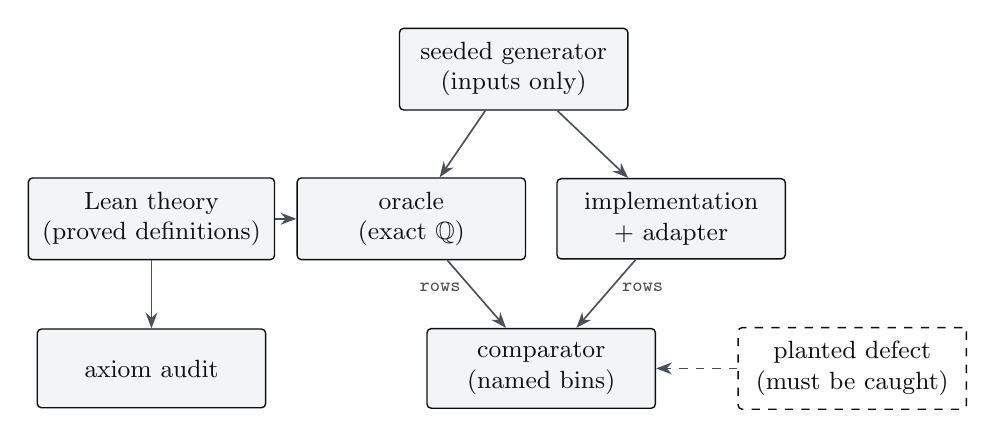
\begin{tikzpicture}[
  box/.style={draw=Ink, line width=0.5pt, fill=Surface, text=Ink, rounded corners=1.5pt,
    align=center, font=\small, inner sep=5pt, minimum height=10mm, minimum width=29mm},
  arr/.style={-{Stealth[length=2mm]}, line width=0.6pt, draw=InkMuted},
  lab/.style={font=\ttfamily\scriptsize, text=InkMuted}]
\node[box] (gen) at (4.6,1.9) {seeded generator\\(inputs only)};
\node[box] (theory) at (0,0) {Lean theory\\(proved definitions)};
\node[box] (oracle) at (3.3,0) {oracle\\(exact $\mathbb{Q}$)};
\node[box] (impl) at (6.6,0) {implementation\\+ adapter};
\node[box] (cmp) at (4.95,-1.9) {comparator\\(named bins)};
\node[box] (audit) at (0,-1.9) {axiom audit};
\node[box, dashed, fill=Background] (planted) at (8.9,-1.9) {planted defect\\(must be caught)};
\draw[arr] (gen) -- (oracle);
\draw[arr] (gen) -- (impl);
\draw[arr] (theory) -- (oracle);
\draw[arr] (theory) -- (audit);
\draw[arr] (oracle) -- node[left, lab, pos=0.4] {rows} (cmp);
\draw[arr] (impl) -- node[right, lab, pos=0.4] {rows} (cmp);
\draw[arr, dashed] (planted) -- (cmp);
\end{tikzpicture}
\caption{The measurement procedure. The generator never computes expected results;
those come only from the oracle.}
\label{fig:harness}
\end{figure}

The procedure follows \texttt{ledger-semantics} (\cref{fig:harness}). A seeded
generator writes case files containing inputs only. It favors the inputs where
implementations are known to have conventions: tied logits, words that are
themselves tokens, and merge tables with several splits of one string. A small
adapter per implementation runs the same cases and prints the oracle's row format.
The comparator places every case in exactly one named bin (agree, diverge, skipped
by either side, or missing), so nothing is dropped silently. Token rows are compared
as strings. Sampler rows require that a zero be matched by a zero and that nonzero
probabilities agree within $10^{-6}$, since llama.cpp stores logits in
\texttt{float32}. Each comparator is observed to fail: a planted defect, an adapter
that glues two tokens or one that inverts temperature, must be detected or the run
fails.

\paragraph{Tie divergences.} An implementation that keeps exactly $k$ tokens breaks
ties in its own order, which need not be the oracle's order by index. Every filter
treats tied tokens alike except for that choice, and tied tokens stay tied through
temperature and renormalization. Such an implementation must therefore agree with
the positional semantics up to a permutation of tied tokens. The harness checks
exactly this: the multiset of (logit, probability) pairs over the kept tokens must
equal that of the oracle's \texttt{q} rows. A divergence that fails this check is
reported as unexplained.

\begin{table}[t]
\centering\small
\caption{Measurements (\texttt{harness/run.sh 600}: four seeds of 600 cases each per
corpus). Lean 4.34.1, Mathlib v4.34.1, \texttt{tokenizers} 0.23.3, \texttt{tiktoken}
0.14.0, llama.cpp commit \texttt{a9d27ac} (2026-10-11).}
\label{tab:results}
\begin{tabularx}{\linewidth}{@{}>{\raggedright\arraybackslash}p{4.6cm}>{\raggedright\arraybackslash}X>{\raggedright\arraybackslash}X@{}}
\toprule
\qpth{Implementation} & \qpth{Compared against} & \qpth{Result}\\
\midrule
HF \texttt{tokenizers}, BPE, defaults & rule-rank BPE (\lean{bpe}) & 13{,}779 / 13{,}779 words identical\\
HF \texttt{tokenizers}, \lean{ignore_merges} & lookup, then rule-rank BPE & 13{,}779 / 13{,}779 identical\\
\texttt{tiktoken} & lookup, then concatenation-rank BPE & 13{,}779 / 13{,}779 identical\\
llama.cpp \lean{top_k}, \lean{top_p}, \lean{min_p}, \texttt{temp}, no ties & tie-keeping filters & 1{,}216 / 1{,}216 chains, $|\Delta p|\le5.1\times10^{-8}$\\
llama.cpp, with ties & tie-keeping, else positional & 939 + 245 / 1{,}184 chains; 0 unexplained\\
Planted defects (tokenizer, sampler) & --- & both detected\\
\bottomrule
\end{tabularx}
\end{table}

\Cref{tab:results} summarizes the results. Two findings came out of the
comparisons. First, \texttt{tiktoken} initially disagreed with the oracle's
concatenation-rank BPE on words that are themselves vocabulary tokens. The
disagreement was a convention, whole-word lookup. Following the
\texttt{ledger-semantics} rule that a divergence is either a defect in the
implementation or a convention the semantics has not yet recorded, we recorded it
as \lean{lookupFirst}, with its own theorems, after which agreement is exact.
Second, on the same random merge tables the two tokenizer libraries disagree with
each other on 439 of 13{,}779 words (3.2\%), and on 279 when Hugging Face uses
\lean{ignore_merges}. The oracle reproduces each library exactly, so every one of
these disagreements is predicted. \Cref{thm:bpeconv} states the condition under which
they cannot occur.

For sampling, llama.cpp agrees with the tie-keeping semantics on every tie-free
chain. On chains with ties, 245 of 1{,}184 diverge, and every one agrees with the
positional semantics up to a permutation of tied tokens. Some of these divergences
cascade: a tie cut by top-$k$ changes the renormalized masses that a later top-$p$
sees. A check that compared kept sets only after the fact would misclassify such
cases. Replaying the convention exactly classifies all of them.

% ===========================================================================
\section{Related work}

\paragraph{Formal methods for machine learning.} Most verification work on neural
networks proves properties of trained models, for example with SMT-based
methods~\cite{katz2017reluplex}. We verify the model-independent algorithms around
the model instead, and connect them to implementations through an oracle. The
denotational method follows Elliott~\cite{elliott2009denotational}. The use of a
proved semantics as a test oracle, the procedure of planted defects, and the
discipline of named skip bins follow \texttt{ledger-semantics}~\cite{ledgersemantics}.
Our category of finite stochastic maps is a special case of Fritz's Markov
categories~\cite{fritz2020markov}.

\paragraph{Tokenization.} Zouhar et al.\ give a formal analysis of BPE as an
optimization problem~\cite{zouhar2023bpe}. Gastaldi et al.\ treat tokenizers as
stochastic maps and study consistency of estimators~\cite{gastaldi2024foundations}.
Vieira et al.\ show how to turn token-level models into character-level
ones~\cite{vieira2024tokens}, which requires exactly the enumeration of
tokenizations we verify. Our no-compression theorem and the agreement criterion
between BPE conventions complement this work at the level of exact identities.

\paragraph{Decoding.} Top-$k$~\cite{fan2018hierarchical}, nucleus~\cite{holtzman2020curious}
and min-$p$~\cite{nguyen2025minp} sampling are usually specified by an algorithm over
sorted arrays, which leaves ties unspecified. \Cref{thm:topk} shows that this gap
cannot be closed by any symmetric rule. Speculative
sampling~\cite{leviathan2023speculative,chen2023speculative} is known to be lossless,
and its acceptance rate is the maximal-coupling bound~\cite{lindvall1992coupling}. Du et
al.\ characterize tightness measure-theoretically~\cite{du2023tight}. We give a
finite-depth statement and an explicit non-tight model.

\paragraph{Attention and inference systems.} Online softmax~\cite{milakov2018online}
underlies FlashAttention~\cite{dao2022flashattention} and its successors, and
KV caching is standard in serving systems~\cite{pope2023scaling,kwon2023vllm}. Our
contribution is the algebraic packaging, a commutative monoid with a free-monoid
homomorphism, and machine-checked proofs over arbitrary exponential characters.
Permutation equivariance of attention without positional encodings is
known~\cite{yun2020universal}.

\paragraph{Masked diffusion.} The time-independence of the optimal denoiser was
observed by Ou et al.~\cite{ou2025absorbing}, in the setting of
D3PM~\cite{austin2021d3pm}, MDLM~\cite{sahoo2024mdlm} and related
models~\cite{shi2024masked,nie2025llada}. We machine-check it, together with the
any-order chain rule and the inexactness of parallel unmasking.

% ===========================================================================
\section{Limitations}

Analysis on the reals enters only through exponential characters, and there is no
measure theory, so sampling and tightness are stated through finite quantities. The
oracle's temperature is restricted to $1/n$, which keeps softmax rational. The
theorems hold for every temperature, but the oracle cannot evaluate an irrational
softmax. Speculative decoding is proved for one drafted token. The sequence version
follows by induction and is not yet formalized. Nothing is proved about
floating-point arithmetic: implementations are compared with exact values within a
stated tolerance. A decision that lies exactly on a floating-point boundary could in
principle diverge, and none occurred in our runs. The diffusion theory covers
absorbing diffusion, not Gaussian diffusion. The chat protocol models tool calling in
its common request-and-result form, not any vendor's specification. The measurements
cover tokenizers and samplers; attention kernels, speculative decoders, chat
renderers and diffusion samplers are evaluated by the oracle but not yet compared
against implementations.

% ===========================================================================
\section{Conclusion}

The inference side of LLMs is small enough to be given a precise meaning and large
enough that its implementations disagree. A machine-checked semantics separates
what is meaning from what is convention. It proves which reorderings, cachings and
tilings are harmless, and it shows that some properties folklore expects, such as
symmetric exact top-$k$, compositional compressing tokenizers and unambiguous plain-text
templates, cannot exist. Connected to an exact oracle, the same definitions become
a test instrument. Every divergence it surfaces is either a defect in an
implementation or a convention that belongs in the semantics.

\paragraph{Availability.} The Lean development, oracle, harness, and recorded
measurement log accompany this paper.

\paragraph{Acknowledgments.} The structure of this work follows
\texttt{ledger-semantics} by John Wiegley. The formalization and harness were
developed with the assistance of an AI system (Claude, Anthropic).

% ===========================================================================
\begin{thebibliography}{99}\small

\bibitem{austin2021d3pm}
J.~Austin, D.~D. Johnson, J.~Ho, D.~Tarlow, and R.~van~den Berg.
\newblock Structured denoising diffusion models in discrete state-spaces.
\newblock In \emph{NeurIPS}, 2021.

\bibitem{chen2023speculative}
C.~Chen, S.~Borgeaud, G.~Irving, J.-B. Lespiau, L.~Sifre, and J.~Jumper.
\newblock Accelerating large language model decoding with speculative sampling.
\newblock arXiv:2302.01318, 2023.

\bibitem{dao2022flashattention}
T.~Dao, D.~Y. Fu, S.~Ermon, A.~Rudra, and C.~R{\'e}.
\newblock {FlashAttention}: Fast and memory-efficient exact attention with {IO}-awareness.
\newblock In \emph{NeurIPS}, 2022.

\bibitem{demoura2021lean4}
L.~de~Moura and S.~Ullrich.
\newblock The {Lean} 4 theorem prover and programming language.
\newblock In \emph{CADE-28}, 2021.

\bibitem{du2023tight}
L.~Du, L.~Torroba~Hennigen, T.~Pimentel, C.~Meister, J.~Eisner, and R.~Cotterell.
\newblock A measure-theoretic characterization of tight language models.
\newblock In \emph{ACL}, 2023.

\bibitem{elliott2009denotational}
C.~Elliott.
\newblock Denotational design with type class morphisms.
\newblock Technical Report 2009-01, LambdaPix, 2009.

\bibitem{fan2018hierarchical}
A.~Fan, M.~Lewis, and Y.~Dauphin.
\newblock Hierarchical neural story generation.
\newblock In \emph{ACL}, 2018.

\bibitem{fritz2020markov}
T.~Fritz.
\newblock A synthetic approach to {Markov} kernels, conditional independence and theorems on sufficient statistics.
\newblock \emph{Advances in Mathematics}, 370, 2020.

\bibitem{gastaldi2024foundations}
J.~L. Gastaldi, J.~Terilla, L.~Malagutti, B.~DuSell, T.~Vieira, and R.~Cotterell.
\newblock The foundations of tokenization: Statistical and computational concerns.
\newblock arXiv:2407.11606, 2024.

\bibitem{greshake2023injection}
K.~Greshake, S.~Abdelnabi, S.~Mishra, C.~Endres, T.~Holz, and M.~Fritz.
\newblock Not what you've signed up for: Compromising real-world {LLM}-integrated applications with indirect prompt injection.
\newblock In \emph{AISec}, 2023.

\bibitem{holtzman2020curious}
A.~Holtzman, J.~Buys, L.~Du, M.~Forbes, and Y.~Choi.
\newblock The curious case of neural text degeneration.
\newblock In \emph{ICLR}, 2020.

\bibitem{katz2017reluplex}
G.~Katz, C.~Barrett, D.~L. Dill, K.~Julian, and M.~J. Kochenderfer.
\newblock Reluplex: An efficient {SMT} solver for verifying deep neural networks.
\newblock In \emph{CAV}, 2017.

\bibitem{kwon2023vllm}
W.~Kwon, Z.~Li, S.~Zhuang, Y.~Sheng, L.~Zheng, C.~H. Yu, J.~E. Gonzalez, H.~Zhang, and I.~Stoica.
\newblock Efficient memory management for large language model serving with {PagedAttention}.
\newblock In \emph{SOSP}, 2023.

\bibitem{ledgersemantics}
J.~Wiegley.
\newblock ledger-semantics: Mathematical semantics of {Ledger}, the double-entry accounting tool.
\newblock \url{https://github.com/ledger/ledger-semantics}, 2026.

\bibitem{leviathan2023speculative}
Y.~Leviathan, M.~Kalman, and Y.~Matias.
\newblock Fast inference from transformers via speculative decoding.
\newblock In \emph{ICML}, 2023.

\bibitem{lindvall1992coupling}
T.~Lindvall.
\newblock \emph{Lectures on the Coupling Method}.
\newblock Wiley, 1992.

\bibitem{liu2023ring}
H.~Liu, M.~Zaharia, and P.~Abbeel.
\newblock Ring attention with blockwise transformers for near-infinite context.
\newblock arXiv:2310.01889, 2023.

\bibitem{mathlib2020}
The mathlib Community.
\newblock The {Lean} mathematical library.
\newblock In \emph{CPP}, 2020.

\bibitem{milakov2018online}
M.~Milakov and N.~Gimelshein.
\newblock Online normalizer calculation for softmax.
\newblock arXiv:1805.02867, 2018.

\bibitem{nguyen2025minp}
M.~N. Nguyen, A.~Baker, C.~Neo, A.~Roush, A.~Kirsch, and R.~Shwartz-Ziv.
\newblock Turning up the heat: Min-p sampling for creative and coherent {LLM} outputs.
\newblock In \emph{ICLR}, 2025.

\bibitem{nie2025llada}
S.~Nie, F.~Zhu, Z.~You, X.~Zhang, J.~Ou, J.~Hu, J.~Zhou, Y.~Lin, J.-R. Wen, and C.~Li.
\newblock Large language diffusion models.
\newblock arXiv:2502.09992, 2025.

\bibitem{ou2025absorbing}
J.~Ou, S.~Nie, K.~Xue, F.~Zhu, J.~Sun, Z.~Li, and C.~Li.
\newblock Your absorbing discrete diffusion secretly models the conditional distributions of clean data.
\newblock In \emph{ICLR}, 2025.

\bibitem{pope2023scaling}
R.~Pope, S.~Douglas, A.~Chowdhery, J.~Devlin, J.~Bradbury, J.~Heek, K.~Xiao, S.~Agrawal, and J.~Dean.
\newblock Efficiently scaling transformer inference.
\newblock In \emph{MLSys}, 2023.

\bibitem{rabe2021selfattention}
M.~N. Rabe and C.~Staats.
\newblock Self-attention does not need {$O(n^2)$} memory.
\newblock arXiv:2112.05682, 2021.

\bibitem{radford2019gpt2}
A.~Radford, J.~Wu, R.~Child, D.~Luan, D.~Amodei, and I.~Sutskever.
\newblock Language models are unsupervised multitask learners.
\newblock OpenAI technical report, 2019.

\bibitem{sahoo2024mdlm}
S.~S. Sahoo, M.~Arriola, Y.~Schiff, A.~Gokaslan, E.~Marroquin, J.~T. Chiu, A.~Rush, and V.~Kuleshov.
\newblock Simple and effective masked diffusion language models.
\newblock In \emph{NeurIPS}, 2024.

\bibitem{sennrich2016bpe}
R.~Sennrich, B.~Haddow, and A.~Birch.
\newblock Neural machine translation of rare words with subword units.
\newblock In \emph{ACL}, 2016.

\bibitem{shi2024masked}
J.~Shi, K.~Han, Z.~Wang, A.~Doucet, and M.~K. Titsias.
\newblock Simplified and generalized masked diffusion for discrete data.
\newblock In \emph{NeurIPS}, 2024.

\bibitem{vieira2024tokens}
T.~Vieira, B.~LeBrun, M.~Giulianelli, J.~L. Gastaldi, B.~DuSell, J.~Terilla, T.~J. O'Donnell, and R.~Cotterell.
\newblock From language models over tokens to language models over characters.
\newblock arXiv:2412.03719, 2024.

\bibitem{wolf2020transformers}
T.~Wolf et~al.
\newblock Transformers: State-of-the-art natural language processing.
\newblock In \emph{EMNLP: System Demonstrations}, 2020.

\bibitem{xiao2024sinks}
G.~Xiao, Y.~Tian, B.~Chen, S.~Han, and M.~Lewis.
\newblock Efficient streaming language models with attention sinks.
\newblock In \emph{ICLR}, 2024.

\bibitem{yun2020universal}
C.~Yun, S.~Bhojanapalli, A.~S. Rawat, S.~J. Reddi, and S.~Kumar.
\newblock Are transformers universal approximators of sequence-to-sequence functions?
\newblock In \emph{ICLR}, 2020.

\bibitem{zouhar2023bpe}
V.~Zouhar, C.~Meister, J.~L. Gastaldi, L.~Du, T.~Vieira, M.~Sachan, and R.~Cotterell.
\newblock A formal perspective on byte-pair encoding.
\newblock In \emph{Findings of ACL}, 2023.

\end{thebibliography}

\end{document}
